\documentclass[11pt]{book}
\oddsidemargin 0in
\evensidemargin 0in
\marginparwidth 0in
\textheight 8in
\textwidth 6.5in
\topmargin 0in
\headheight 14pt
\usepackage{amssymb,amsmath,amsthm,fancyhdr,supertabular,longtable,hhline}
\usepackage{colortbl}
\usepackage{import, multicol,boxedminipage}
\usepackage{chapterfolder}
\usepackage[metapost,truebbox]{mfpic}
\usepackage[pdflatex]{graphicx}
\usepackage{makeidx}
\usepackage[colorlinks, hyperindex, plainpages=false, linkcolor=blue, urlcolor=blue, pdfpagelabels]{hyperref}
\usepackage[all]{hypcap}
\usepackage{cancel}
\usepackage{sectsty}
\usepackage{textcomp}
\allsectionsfont{\mdseries \scshape}
\definecolor{ResultColor}{gray}{0.9}
\theoremstyle{definition}  % this prevents the text in definitions, theorems, and corollaries from being italicized
\newtheorem{defn}{\sc Definition}[chapter]
\newtheorem{thm}{\sc Theorem}[chapter]
\newtheorem{cor}[thm]{\sc Corollary}
\newtheorem{eqn}{\sc Equation}[chapter]
\newtheorem{ex}{\sc Example}[section]
\newtheorem{fig}{\sc Figure}[chapter]
\setlength{\parindent}{0in}
\newcommand{\bbm}{\begin{boxedminipage}{6.41in}}
\newcommand{\ebm}{\end{boxedminipage}}
\usepackage{array}
\setlength{\extrarowheight}{2pt}
\allowdisplaybreaks[2]
\newcounter{HW}
\newcounter{HWindent}

\begin{document}

\chapter{\sc Introduction to Trigonometry}

\section{Angles and their Measure}

\mfpicnumber{1}

\opengraphsfile{Angles}

\setcounter{footnote}{0}

\label{Angles}

This section begins our study of Trigonometry and to get started, we recall some basic definitions from Geometry.  A \index{ray ! definition of} \textbf{ray} is usually described as a `half-line' and can be thought of as a line segment in which one of the two endpoints is pushed off infinitely distant from the other, as pictured below.  The point from which the ray originates is called the \index{ray ! initial point} \textbf{initial point} of the ray.

\begin{center}

\begin{mfpic}[15]{-1}{7}{-1}{3}
\arrow \polyline{(0,0), (7,2)}
\point[3pt]{(0,0)}
\tlabel[cc](-0.25,-0.5){\scriptsize $P$}
\tcaption{A ray with initial point $P$.}
\end{mfpic}

\end{center}

When two rays share a common initial point they form an \index{angle ! definition} \textbf{angle} and the common initial point is called the \index{angle ! vertex}\index{vertex ! of an angle}\textbf{vertex} of the angle.  Two  examples of what are commonly thought of as angles are

\[ \begin{array}{cc}

\begin{mfpic}[15]{-5}{5}{-3}{3}
\arrow \reverse \arrow \polyline{(-5,2), (0,0), (5,2)}
\point[3pt]{(0,0)}
\tlabel[cc](-0.1,-0.5){\scriptsize $P$}
\tcaption{An angle with vertex $P$.}
\end{mfpic}  

&

\hspace{1.75in}

\begin{mfpic}[15]{-5}{7}{-3}{3}
\arrow \reverse \arrow \polyline{(7,2), (0,0), (7,-2)}
\point[3pt]{(0,0)}
\tlabel[cc](-0.25,-0.5){\scriptsize $Q$}
\tcaption{An angle with vertex $Q$.}
\end{mfpic}   \\ \end{array} \]

However, the two figures below also depict angles - albeit these are, in some sense, extreme cases.  In the first case, the two rays are directly opposite each other forming what is known as a \index{angle ! straight}\index{straight angle}\textbf{straight angle}; in the second, the rays are identical so the `angle' is indistinguishable from the ray itself.

\[ \begin{array}{cc}

\begin{mfpic}[15]{-5}{5}{-3}{3}
\arrow \reverse \arrow \polyline{(-5,0), (5,0)}
\point[3pt]{(0,0)}
\tlabel[cc](-0.1,-0.5){\scriptsize $P$}
\tcaption{A straight angle.}
\end{mfpic}  

&

\hspace{1.75in}

\begin{mfpic}[15]{-5}{7}{-3}{3}
\arrow  \polyline{(0,0), (7,-2)}
\point[3pt]{(0,0)}
\tlabel[cc](-0.25,-0.5){\scriptsize $Q$}
\end{mfpic}   \\ \end{array} \]

The \index{angle ! measurement}\index{measure of an angle}\textbf{measure of an angle} is a number which indicates the amount of rotation that separates the rays of the angle.  There is one immediate problem with this, as pictured below. 

\[ \begin{array}{cc}

\begin{mfpic}[15]{-5}{5}{-3}{3}
\arrow \reverse \arrow \polyline{(5,2), (0,0), (5,-2)}
\point[3pt]{(0,0)}
\arrow \reverse \arrow \arc[c]{(0,0), (2.5,-0.9), 40}
\drawcolor{white} \arc[c]{(0,0), (2.4,-1.1), -310}
\end{mfpic}  

& 

\hspace{2in}

\begin{mfpic}[15]{-5}{5}{-3}{3}
\arrow \reverse \arrow \polyline{(5,2), (0,0), (5,-2)}
\point[3pt]{(0,0)}
\arrow \reverse \arrow \arc[c]{(0,0), (2.4,-1.1), -310}
\end{mfpic} \\ \end{array} \]

Which amount of rotation are we attempting to quantify?  What we have just discovered is that we have at least two angles described by this diagram.\footnote{The phrase `at least' will be justified in short order.}  Clearly these two angles have different measures because one appears to represent a larger rotation than the other, so we must label them differently.  In this book, we use lower case Greek letters such as $\alpha$ (alpha),   $\beta$ (beta),  $\gamma$ (gamma) and $\theta$ (theta) to label angles.  So, for instance, we have

\[ \begin{mfpic}[15]{-5}{5}{-3}{3}
\arrow \reverse \arrow \polyline{(5,2), (0,0), (5,-2)}
\point[3pt]{(0,0)}
\arrow \reverse \arrow \arc[c]{(0,0), (2.5,-0.9), 40}
\tlabel[cc](3,0){\scriptsize{$\alpha$}}
\arrow \reverse \arrow \arc[c]{(0,0), (2.4,-1.1), -310}
\tlabel[cc](-3,0){\scriptsize{$\beta$}}
\end{mfpic}  \]

One commonly used system to measure angles is \index{angle ! degree}\index{degree measure}\textbf{degree measure}.  Quantities measured in degrees are denoted by the familiar `$^{\circ}$' symbol.  One complete revolution as shown below is $360^{\circ}$, and parts of a revolution are measured proportionately.\footnote{The choice of `$360$' is most often attributed to the \href{http://en.wikipedia.org/wiki/Degree_(angle)}{\underline{Babylonians}}.}  Thus half of a revolution (a straight angle) measures $\frac{1}{2} \left(360^{\circ}\right) = 180^{\circ}$, a quarter of a revolution (a \index{right angle}\index{angle ! right}\textbf{right angle}) measures $\frac{1}{4} \left(360^{\circ}\right) = 90^{\circ}$ and so on.

\[ \begin{array}{ccc}

\begin{mfpic}[15]{-5}{5}{-3}{3}
\arrow  \polyline{(0,0), (5,0)}
\point[3pt]{(0,0)}
\arrow \reverse \arrow \arc[c]{(0,0), (2.5,0.1), 355}
\tcaption{One revolution $\leftrightarrow 360^{\circ}$}
\end{mfpic} 

&

\hspace{.5in}

\begin{mfpic}[15]{-5}{5}{-3}{3}
\arrow \reverse \arrow  \polyline{(-5,0), (5,0)}
\point[3pt]{(0,0)}
\arrow \reverse \arrow \arc[c]{(0,0), (2.5,0.1), 175}
\drawcolor{white} \arc[c]{(0,0), (2.5,-0.1), -175}
\tcaption{$180^{\circ}$}
\end{mfpic} 

&

\hspace{.5in}

\begin{mfpic}[15]{-5}{5}{-3}{5}
\arrow \reverse \arrow  \polyline{(0,5), (0,0),  (5,0)}
\point[3pt]{(0,0)}
\arrow \reverse \arrow \arc[c]{(0,0), (2.5,0.1), 85}
\polyline{(0,0.5), (0.5,0.5), (0.5,0)}
\drawcolor{white} \arc[c]{(0,0), (2.5,-0.1), -265}
\tcaption{$90^{\circ}$}
\end{mfpic} 

\\  \end{array} \]

Note that in the above figure,  we have used the small square `$\! \! \! \! \! \! \qed$' to denote a right angle, as is commonplace in Geometry.  Recall that if an angle measures strictly between $0^{\circ}$ and $90^{\circ}$ it is called an \index{acute angle}\index{angle ! acute}\textbf{acute angle} and if it measures strictly between $90^{\circ}$ and $180^{\circ}$ it is called an \index{obtuse angle}\index{angle ! obtuse}\textbf{obtuse angle}. It is important to note that, theoretically, we can know the measure of any angle as long as we know the proportion it represents of entire revolution.\footnote{This is how a protractor is graded.}  For instance, the measure of an angle which represents a rotation of $\frac{2}{3}$ of a revolution would measure $\frac{2}{3} \left(360^{\circ}\right) = 240^{\circ}$,  the measure of an angle which constitutes only $\frac{1}{12}$ of a revolution measures $\frac{1}{12} \left(360^{\circ}\right) = 30^{\circ}$ and an angle which indicates no rotation at all is measured as $0^{\circ}$.

\[ \begin{array}{ccc}

\begin{mfpic}[15]{-5}{5}{-5}{5}
\arrow \reverse \arrow \polyline{(-2.5,-4.33), (0,0), (5,0)}
\point[3pt]{(0,0)}
\arrow \reverse \arrow \arc[c]{(0,0), (2.5,0.1), 235}
\tcaption{$240^{\circ}$}
\end{mfpic} 

&

\hspace{.5in}

\begin{mfpic}[15]{-5}{5}{-5}{5}
\drawcolor{white}
\polyline{(-2.5,-4.33), (0,0), (5,0)}
\arc[c]{(0,0), (2.5,0.1), 235}
\drawcolor{black}
\arrow \reverse \arrow  \polyline{(4.33, 2.5), (0,0), (5,0)}
\point[3pt]{(0,0)}
\arrow \reverse \arrow \arc[c]{(0,0), (2.5,0.1), 25}
\tcaption{$30^{\circ}$}
\end{mfpic} 

&

\hspace{.5in}

\begin{mfpic}[15]{-5}{5}{-5}{5}
\drawcolor{white}
\polyline{(-2.5,-4.33), (0,0), (5,0)}
\arc[c]{(0,0), (2.5,0.1), 235}
\drawcolor{black}
\arrow \polyline{(0,0), (5,0)}
\point[3pt]{(0,0)}
\tcaption{$0^{\circ}$}
\end{mfpic} 

\\  \end{array} \]

Using our definition of degree measure, we have that $1^{\circ}$ represents the measure of an angle which constitutes $\frac{1}{360}$ of a revolution.  Even though it may be hard to draw, it is nonetheless not difficult to imagine an angle with measure smaller than $1^{\circ}$.  There are two ways to subdivide degrees.  The first, and most familiar, is \index{decimal degrees}\index{angle ! decimal degrees}\textbf{decimal degrees}.  For example, an angle with a measure of $30.5^{\circ}$ would represent a rotation halfway between $30^{\circ}$ and $31^{\circ}$, or equivalently, $\frac{30.5}{360} = \frac{61}{720}$ of a full rotation.  This can be taken to the limit using Calculus so that measures like $\sqrt{2}^{\, \circ}$ make sense.\footnote{Awesome math pun aside, this is the same idea behind defining irrational exponents in Section \ref{IntroExpLogs}.}  The second way to divide degrees is the \index{angle ! DMS}\index{DMS}\textbf{Degree - Minute - Second} (\textbf{DMS}) system.  In this system, one degree is divided equally into sixty minutes, and in turn, each minute is divided equally into sixty seconds.\footnote{Does this kind of system seem familiar?}  In symbols, we write $1^{\circ} = 60'$ and $1' = 60''$, from which it follows that  $1^{\circ} = 3600''$.  To convert a measure of $42.125^{\circ}$ to the DMS system, we start by noting that $42.125^{\circ} = 42^{\circ} + 0.125^{\circ}$. Converting the partial amount of degrees to minutes, we find $0.125^{\circ} \left( \frac{60'}{1^{\circ}} \right) = 7.5' = 7' + 0.5'$. Converting the partial amount of minutes to seconds gives  $0.5' \left(\frac{60''}{1'} \right) = 30''$.  Putting it all together yields 

\[ \begin{array}{rcl}

42.125^{\circ} & = &  42^{\circ} + 0.125^{\circ} \\
               & = & 42^{\circ} + 7.5' \\
               & = & 42^{\circ} + 7' + 0.5' \\
               & = & 42^{\circ} + 7' + 30'' \\
               & = & 42^{\circ} 7' 30'' \\ \end{array} \]
      
On the other hand, to convert $117^{\circ}15'45''$ to decimal degrees, we first compute $15' \left(\frac{1^{\circ}}{60'}\right) = \frac{1}{4}^{\circ}$ and $45'' \left(\frac{1^{\circ}}{3600''}\right) = \frac{1}{80}^{\circ}$. Then we find

\[ \begin{array}{rcl}

 117^{\circ}15'45'' & = & 117^{\circ} + 15' + 45'' \\ [5pt]
                    & = & 117^{\circ} + \frac{1}{4}^{\circ} + \frac{1}{80}^{\circ} \\ [5pt]
                    & = & \frac{9381}{80}^{\circ} \\ [5pt]
                    & = &  117.2625^{\circ} \\ \end{array} \]

Recall that two acute angles are called \index{complementary angles}\index{angle ! complementary}\textbf{complementary angles} if their measures add to $90^{\circ}$.  Two angles, either a pair of right angles or one acute angle and one obtuse angle, are called \index{supplementary angles}\index{angle ! supplementary}\textbf{supplementary angles} if their measures add to $180^{\circ}$. In the diagram below,  the angles $\alpha$ and $\beta$ are supplementary angles while the pair $\gamma$ and $\theta$ are complementary angles. 

\[ \begin{array}{cc}

\begin{mfpic}[15]{-5}{5}{-5}{5}
\arrow \reverse \arrow  \polyline{(-5,0), (5,0)}
\arrow \polyline{(0,0),  (4.33, 2.5)}
\point[3pt]{(0,0)}
\arrow \reverse \arrow \arc[c]{(0,0), (2.5,0.1), 25}
\arrow \reverse \arrow \arc[c]{(0,0), (-2.5,0.1), -145}
\tlabel[cc](3,0.75){\scriptsize{$\alpha$}}
\tlabel[cc](-0.5,3){\scriptsize{$\beta$}}
\tcaption{Supplementary Angles}
\end{mfpic} 

&

\hspace{1in}

\begin{mfpic}[15]{-5}{6}{-5}{5}
\arrow \reverse \arrow  \polyline{(0,5), (0,0), (6,0)}
\arrow \polyline{(0,0),  (4.33, 2.5)}
\point[3pt]{(0,0)}
\arrow \reverse \arrow \arc[c]{(0,0), (2.5,0.1), 25}
\arrow \reverse \arrow \arc[c]{(0,0), (0.1,2.5), -55}
\tlabel[cc](3,0.75){\scriptsize{$\gamma$}}
\tlabel[cc](1.5,2.5){\scriptsize{$\theta$}}
\tcaption{Complementary Angles}
\end{mfpic} 

\\  \end{array} \]

In practice, the distinction between the angle itself and its measure is blurred so that the sentence `$\alpha$ is an angle measuring $42^{\circ}$' is often abbreviated as `$\alpha = 42^{\circ}$.'  It is now time for an example.

\begin{ex} \label{degreeex}  Let $\alpha = 111.371^{\circ}$  and $\beta = 37^{\circ}28'17''$.

\begin{enumerate}

\item  Convert $\alpha$ to the DMS system.  Round your answer to the nearest second.

\item  Convert $\beta$ to decimal degrees.  Round your answer to the nearest thousandth of a degree.

\item  Sketch $\alpha$ and $\beta$.

\item  Find a supplementary angle for $\alpha$.

\item  Find a complementary angle for $\beta$.

\end{enumerate}

{\bf Solution.}

\begin{enumerate}

\item  To convert $\alpha$ to the DMS system, we start with $111.371^{\circ} = 111^{\circ}+ 0.371^{\circ}$.  Next we convert $0.371^{\circ} \left(\frac{60'}{1^{\circ}}\right) = 22.26'$.  Writing $22.26' = 22'+ 0.26'$, we convert $0.26' \left( \frac{60''}{1'} \right) = 15.6''$.  Hence,

\[ \begin{array}{rcl}

111.371^{\circ} & = & 111^{\circ} + 0.371^{\circ} \\
                & = & 111^{\circ} + 22.26' \\
                & = & 111^{\circ} + 22' + 0.26' \\
                & = & 111^{\circ} + 22' + 15.6'' \\
                & = & 111^{\circ}22'15.6'' \\ \end{array} \]

Rounding to seconds, we obtain $\alpha \approx 111^{\circ}22'16''$.

\item  To convert $\beta$ to decimal degrees, we convert $28' \left(\frac{1^{\circ}}{60'}\right) = \frac{7}{15}^{\, \circ}$ and $17''\left(\frac{1^{\circ}}{3600'}\right) = \frac{17}{3600}^{\, \circ}$.  Putting it all together, we have

\[ \begin{array}{rcl}

 37^{\circ}28'17'' & = & 37^{\circ} + 28' + 17'' \\ [5pt]
                   & = & 37^{\circ} +  \frac{7}{15}^{\, \circ} + \frac{17}{3600}^{\, \circ} \\ [5pt]
                   & = & \frac{134897}{3600}^{\circ} \\ [5pt]
                   & \approx & 37.471^{\circ} \\ \end{array} \]

\item  To sketch $\alpha$, we first note that $90^{\circ} < \alpha < 180^{\circ}$.  If we divide this range in half, we get $90^{\circ} < \alpha < 135^{\circ}$, and once more, we have $90^{\circ} < \alpha < 112.5^{\circ}$.  This gives us a pretty good estimate for $\alpha$, as shown below.\footnote{If this process seems hauntingly familiar, it should. Compare this method to the Bisection Method introduced in Section \ref{RealZeros}.}  Proceeding similarly for $\beta$, we find $0^{\circ} < \beta < 90^{\circ}$, then $0^{\circ} < \beta < 45^{\circ}$, $22.5^{\circ} < \beta < 45^{\circ}$, and lastly, $33.75^{\circ} < \beta < 45^{\circ}$.  

\[ \begin{array}{cc}

\begin{mfpic}[15]{-5}{5}{-5}{5}
\arrow \reverse \arrow  \polyline{(-1.822, 4.656), (0,0), (5,0)}
\dotted \polyline{ (-5,0), (0,0), (0,5)}
\dotted \polyline{ (-3.5355,3.5355), (0,0)}
\dotted \polyline{ (-1.9134,4.6194), (0,0)}
\point[3pt]{(0,0)}
\arrow \reverse \arrow \arc[c]{(0,0), (2.5,0.1), 107}
\tcaption{Angle $\alpha$}
\end{mfpic} 

&

\hspace{1in}

\begin{mfpic}[15]{-5}{5}{-5}{5}
\arrow \reverse \arrow  \polyline{(3.9683, 3.0417), (0,0), (5,0)}
\dotted \polyline{ (0,5), (0,0), (5,0)}
\dotted \polyline{ (3.5355,3.5355), (0,0)}
\dotted \polyline{ (4.6194,1.9134), (0,0)}
\dotted \polyline{ (4.1573,2.7778), (0,0)}
\point[3pt]{(0,0)}
\arrow \reverse \arrow \arc[c]{(0,0), (2.5,0.1), 33}
\tcaption{Angle $\beta$}
\end{mfpic}  \\ \end{array} \]

\item  To find a supplementary angle for $\alpha$, we seek an angle $\theta$ so that $\alpha + \theta = 180^{\circ}$.  We get $\theta = 180^{\circ} - \alpha =  180^{\circ} - 111.371^{\circ} = 68.629^{\circ}$.

\item  To find a complementary  angle for $\beta$, we seek an angle $\gamma$ so that $\beta + \gamma = 90^{\circ}$.  We get $\gamma = 90^{\circ} - \beta =  90^{\circ} - 37^{\circ}28'17''$.  While we could reach for the calculator to obtain an approximate answer, we choose instead to do a bit of sexagesimal\footnote{Like `latus rectum,' this is also a real math term.} arithmetic.  We first rewrite  $90^{\circ} = 90^{\circ} 0' 0'' =  89^{\circ}60' 0'' =  89^{\circ}59'60''$. In essence, we are `borrowing' $1^{\circ} = 60'$ from the degree place,  and then borrowing $1' = 60''$ from the minutes place.\footnote{This is the exact same kind of `borrowing' you used to do in Elementary School when trying to find $300 - 125$. Back then, you were working in a base ten system;  here, it is base sixty.} This yields, $\gamma = 90^{\circ} - 37^{\circ}28'17'' = 89^{\circ}59'60'' - 37^{\circ}28'17'' = 52^{\circ}31'43''$.  \qed

\end{enumerate}

\end{ex} 

Up to this point, we have discussed only angles which measure between $0^{\circ}$ and $360^{\circ}$, inclusive.  Ultimately, we want to use the arsenal of Algebra which we have stockpiled in Chapters \ref{RelationsandFunctions} through \ref{SequencesandSeries} to not only solve geometric problems involving angles, but also to extend their applicability to other real-world phenomena.  A first step in this direction is to extend our notion of `angle' from merely measuring an extent of rotation to quantities which can be associated with real numbers.  To that end, we introduce the concept of an \index{angle ! oriented}\index{oriented angle}\textbf{oriented angle}.  As its name suggests, in an oriented angle, the direction of the rotation is important.  We imagine the angle being swept out starting from an \index{angle ! initial side}\index{initial side of an angle}\textbf{initial side} and ending at a \index{angle ! terminal side}\index{terminal side of an angle}\textbf{terminal side}, as shown below.  When the rotation is counter-clockwise\footnote{`widdershins'} from initial side to terminal side, we say that the angle is \index{angle ! positive}\index{positive angle}\textbf{positive}; when the rotation is clockwise, we say that the angle is \index{angle ! negative}\index{negative angle}\textbf{negative}.

\[ \begin{array}{cc}

\begin{mfpic}[15]{-5}{5}{-5}{5}
\arrow \reverse \arrow  \polyline{(3.5355, 3.5355), (0,0), (5,0)}
\point[3pt]{(0,0)}
\arrow \arc[c]{(0,0), (2.5,0.1), 40}
\tlabel[cc](2, -0.5){\tiny Initial Side}
\tlabel[cc](1.5,2){\tiny \rotatebox{45}{Terminal Side}}
\end{mfpic}

&

\hspace{1.5in}

\begin{mfpic}[15]{-5}{5}{-5}{5}
\arrow \reverse \arrow  \polyline{(3.5355, -3.5355), (0,0), (5,0)}
\point[3pt]{(0,0)}
\arrow \arc[c]{(0,0), (2.5,-0.1), -40}
\tlabel[cc](2, 0.5){\tiny Initial Side}
\tlabel[cc](1.5,-2){\tiny \rotatebox{-45}{Terminal Side}}
\end{mfpic} \\ 

\text{A positive angle, $45^{\circ}$} & \hspace{1.5in} \text{A negative angle, $-45^{\circ}$}

\end{array} \]

At this point, we also extend our allowable rotations to include angles which encompass more than one revolution.  For example, to sketch an angle with measure $450^{\circ}$ we start with an initial side, rotate counter-clockwise one complete revolution (to take care of the `first' $360^{\circ}$) then continue with an additional $90^{\circ}$ counter-clockwise rotation, as seen below.

\begin{center}

\begin{mfpic}[15]{-5}{5}{-3}{5}
\arrow \reverse \arrow  \polyline{(0,5), (0,0),  (5,0)}
\point[3pt]{(0,0)}
\arrow \parafcn{0,445,5}{(t+200)*dir(t)/200} 
\tcaption{$450^{\circ}$}
\end{mfpic} 

\end{center}

To further connect angles with the Algebra which has come before, we shall often overlay an angle diagram on the coordinate plane.  An angle is said to be in \index{angle ! standard position}\index{standard position of an angle}\textbf{standard position} if its vertex is the origin and its initial side coincides with the positive $x$-axis.  Angles in standard position are classified according to where their terminal side lies.  For instance, an angle in standard position whose terminal side lies in Quadrant I is called a `Quadrant I angle'.  If the terminal side of an angle lies on one of the coordinate axes, it is called a \index{angle ! quadrantal}\index{quadrantal angle}\textbf{quadrantal angle}.  Two angles in standard position are called \index{angle ! coterminal}\index{coterminal angle}\textbf{coterminal} if they share the same terminal side.\footnote{Note that by being in standard position they automatically share the same initial side which is the positive $x$-axis.}  In the figure below, $\alpha = 120^{\circ}$ and $\beta = -240^{\circ}$ are two coterminal Quadrant II angles drawn in standard position.    Note that $\alpha = \beta + 360^{\circ}$, or equivalently, $\beta = \alpha - 360^{\circ}$. We leave it as an exercise to the reader to verify that coterminal angles always differ by a multiple of $360^{\circ}$.\footnote{It is worth noting that all of the pathologies of Analytic Trigonometry result from this innocuous fact.} More precisely, if $\alpha$ and $\beta$ are coterminal angles, then $\beta = \alpha + 360^{\circ} \cdot k$ where $k$ is an integer.\footnote{Recall that this means $k = 0, \pm 1, \pm 2, \ldots$.}

\begin{center}

\begin{mfpic}[15]{-5}{5}{-5}{5}
\drawcolor[gray]{0.7}
\axes
\xmarks{-4,-3,-2,-1,1,2,3,4}
\ymarks{-4,-3,-2,-1,1,2,3,4}
\tlabel(5,-0.5){\scriptsize $x$}
\tlabel(0.25,4.75){\scriptsize $y$}
\tlabel(2,2){\scriptsize $\alpha = 120^{\circ}$}
\tlabel(-5,-2){\scriptsize $\beta = -240^{\circ}$}
\drawcolor[rgb]{0.33,0.33,0.33}
\arrow \reverse \polyline{(-2.5, 4.3301), (0,0), (5,0)}
\point[3pt]{(0,0)}
\arrow \arc[c]{(0,0), (2.5,0.1), 115}
\arrow \arc[c]{(0,0), (2.5,-0.1), -235}
\tlpointsep{5pt}
\scriptsize
\axislabels {x}{{$-4 \hspace{7pt}$} -4, {$-3 \hspace{7pt}$} -3, {$-2 \hspace{7pt}$} -2, {$-1 \hspace{7pt}$} -1, {$1$} 1, {$2$} 2, {$3$} 3, {$4$} 4}
\axislabels {y}{{$-1$} -1, {$-2$} -2, {$-3$} -3, {$-4$} -4, {$1$} 1, {$2$} 2, {$3$} 3, {$4$} 4}
\normalsize
\end{mfpic}

Two coterminal angles, $\alpha = 120^{\circ}$ and $\beta = -240^{\circ}$, in standard position.

\end{center}

\begin{ex}  \label{orientedcoterminaldegree} Graph each of the (oriented) angles below in standard position and classify them according to where their terminal side lies. Find three coterminal angles, at least one of which is positive and one of which is negative.

\begin{multicols}{4}

\begin{enumerate}

\item  $\alpha = 60^{\circ}$

\item  $\beta = -225^{\circ}$

\item  $\gamma = 540^{\circ}$

\item  $\phi = -750^{\circ}$

\end{enumerate}

\end{multicols}

{\bf Solution.}  

\begin{enumerate}

\item  To graph $\alpha = 60^{\circ}$, we draw an angle with its initial side on the positive $x$-axis and rotate counter-clockwise $\frac{60^{\circ}}{360^{\circ}} = \frac{1}{6}$ of a revolution.  We see that $\alpha$ is a Quadrant I angle.  To find angles which are coterminal, we look for angles $\theta$ of the form $\theta = \alpha + 360^{\circ} \cdot k$, for some integer $k$.  When $k = 1$, we get $\theta =  60^{\circ} + 360^{\circ} = 420^{\circ}$.   Substituting $k = -1$ gives $\theta = 60^{\circ} - 360^{\circ} = -300^{\circ}$.  Finally, if we let $k = 2$, we get $\theta =  60^{\circ} + 720^{\circ} = 780^{\circ}$.  

\item  Since $\beta = - 225^{\circ}$ is negative, we start at the positive $x$-axis and rotate \textit{clockwise} $\frac{225^{\circ}}{360^{\circ}} = \frac{5}{8}$ of a revolution. We see that $\beta$ is a Quadrant II angle.  To find coterminal angles, we proceed as before and compute $\theta = -225^{\circ} + 360^{\circ} \cdot k$ for integer values of $k$.  We find $135^{\circ}$, $-585^{\circ}$ and $495^{\circ}$ are all coterminal with $-225^{\circ}$.   

\begin{center}

\begin{tabular}{cc}

\begin{mfpic}[15]{-5}{5}{-5}{5}
\drawcolor[gray]{0.7}
\axes
\xmarks{-4,-3,-2,-1,1,2,3,4}
\ymarks{-4,-3,-2,-1,1,2,3,4}
\tlabel(5,-0.5){\scriptsize $x$}
\tlabel(0.25,4.75){\scriptsize $y$}
\tlabel(2.5,1){\scriptsize $\alpha = 60^{\circ}$}
\drawcolor[rgb]{0.33,0.33,0.33}
\arrow \reverse \polyline{(2.5, 4.3301), (0,0), (5,0)}
\point[3pt]{(0,0)}
\arrow \arc[c]{(0,0), (2.5,0.1), 55}
\tlpointsep{5pt}
\scriptsize
\axislabels {x}{{$-4 \hspace{7pt}$} -4, {$-3 \hspace{7pt}$} -3, {$-2 \hspace{7pt}$} -2, {$-1 \hspace{7pt}$} -1, {$1$} 1, {$2$} 2, {$3$} 3, {$4$} 4}
\axislabels {y}{{$-1$} -1, {$-2$} -2, {$-3$} -3, {$-4$} -4, {$1$} 1, {$2$} 2, {$3$} 3, {$4$} 4}
\normalsize
\end{mfpic}

&

\hspace{.5in}

\begin{mfpic}[15]{-5}{5}{-5}{5}
\drawcolor[gray]{0.7}
\axes
\xmarks{-4,-3,-2,-1,1,2,3,4}
\ymarks{-4,-3,-2,-1,1,2,3,4}
\tlabel(5,-0.5){\scriptsize $x$}
\tlabel(0.25,4.75){\scriptsize $y$}
\tlabel(-4.5,-2.5){\scriptsize $\beta = -225^{\circ}$}
\drawcolor[rgb]{0.33,0.33,0.33}
\arrow \reverse \polyline{(-3.801, 3.801), (0,0), (5,0)}
\point[3pt]{(0,0)}
\arrow \arc[c]{(0,0), (2.5,-0.1), -220}
\tlpointsep{5pt}
\scriptsize
\axislabels {x}{{$-4 \hspace{7pt}$} -4, {$-3 \hspace{7pt}$} -3, {$-2 \hspace{7pt}$} -2, {$-1 \hspace{7pt}$} -1, {$1$} 1, {$2$} 2, {$3$} 3, {$4$} 4}
\axislabels {y}{{$-1$} -1, {$-2$} -2, {$-3$} -3, {$-4$} -4, {$1$} 1, {$2$} 2, {$3$} 3, {$4$} 4}
\normalsize
\end{mfpic} 

\\

$\alpha = 60^{\circ}$ in standard position. & \hspace{1in} $\beta = -225^{\circ}$ in standard position.\\

\end{tabular}

\end{center}

\item Since $\gamma = 540^{\circ}$ is positive, we rotate counter-clockwise from the positive $x$-axis.  One full revolution accounts for $360^{\circ}$, with $180^{\circ}$, or $\frac{1}{2}$ of a revolution remaining.  Since the terminal side of $\gamma$ lies on the negative $x$-axis, $\gamma$ is a quadrantal angle.  All angles coterminal with $\gamma$ are of the form $\theta = 540^{\circ} + 360^{\circ} \cdot k$, where $k$ is an integer.  Working through the arithmetic, we find three such angles: $180^{\circ}$, $-180^{\circ}$ and $900^{\circ}$.

\item  The Greek letter $\phi$ is pronounced `fee' or `fie' and since $\phi$ is negative, we begin our rotation clockwise from the positive $x$-axis.  Two full revolutions account for $720^{\circ}$, with just $30^{\circ}$ or $\frac{1}{12}$ of a revolution to go. We find that $\phi$ is a Quadrant IV angle. To find coterminal angles, we compute $\theta = -750^{\circ} +   360^{\circ} \cdot k$ for a few integers $k$ and obtain $-390^{\circ}$, $-30^{\circ}$ and $330^{\circ}$.

\begin{center}

\begin{tabular}{cc}

\begin{mfpic}[15]{-5}{5}{-5}{5}
\drawcolor[gray]{0.7}
\axes
\xmarks{-4,-3,-2,-1,1,2,3,4}
\ymarks{-4,-3,-2,-1,1,2,3,4}
\tlabel(5,-0.5){\scriptsize $x$}
\tlabel(0.25,4.75){\scriptsize $y$}
\tlabel(-4.5,2.5){\scriptsize $\gamma = 540^{\circ}$}
\drawcolor[rgb]{0.33,0.33,0.33}
\arrow \reverse \polyline{(-5,0), (0,0), (5,0)}
\point[3pt]{(0,0)}
\arrow \parafcn{0,535,5}{(t+200)*dir(t)/200} 
\tlpointsep{5pt}
\scriptsize
\axislabels {x}{{$-4 \hspace{7pt}$} -4, {$-3 \hspace{7pt}$} -3, {$-2 \hspace{7pt}$} -2, {$-1 \hspace{7pt}$} -1, {$1$} 1, {$2$} 2, {$3$} 3, {$4$} 4}
\axislabels {y}{{$-1$} -1, {$-2$} -2, {$-3$} -3, {$-4$} -4, {$1$} 1, {$2$} 2, {$3$} 3, {$4$} 4}
\normalsize
\end{mfpic}

&

\hspace{.5in}

\begin{mfpic}[15]{-5}{5}{-5}{5}
\drawcolor[gray]{0.7}
\axes
\xmarks{-4,-3,-2,-1,1,2,3,4}
\ymarks{-4,-3,-2,-1,1,2,3,4}
\tlabel(5,-0.5){\scriptsize $x$}
\tlabel(0.25,4.75){\scriptsize $y$}
\tlabel(0.5,-2.5){\scriptsize $\phi = -750^{\circ}$}
\drawcolor[rgb]{0.33,0.33,0.33}
\arrow \reverse \polyline{(4.3301, -2.5), (0,0), (5,0)}
\point[3pt]{(0,0)}
\arrow \parafcn{0,745,5}{(t+100)*dir(0-t)/400}
\tlpointsep{5pt}
\scriptsize
\axislabels {x}{{$-4 \hspace{7pt}$} -4, {$-3 \hspace{7pt}$} -3, {$-2 \hspace{7pt}$} -2, {$-1 \hspace{7pt}$} -1, {$1$} 1, {$2$} 2, {$3$} 3, {$4$} 4}
\axislabels {y}{{$-1$} -1, {$-2$} -2, {$-3$} -3, {$-4$} -4, {$1$} 1, {$2$} 2, {$3$} 3, {$4$} 4}
\normalsize
\end{mfpic} 

\\

$\gamma = 540^{\circ}$ in standard position. & \hspace{1in} $\phi = -750^{\circ}$ in standard position.   \\

\end{tabular}

\end{center}

\end{enumerate}
\qed

\end{ex}

Note that since there are infinitely many integers, any given angle has infinitely many coterminal angles, and the reader is encouraged to plot the few sets of coterminal angles found in Example \ref{orientedcoterminaldegree} to see this.  We are now just one step away from completely marrying angles with the real numbers and the rest of Algebra.  To that end, we recall this definition from Geometry.

\smallskip

\colorbox{ResultColor}{\bbm

\begin{defn} \label{pidefn} \index{pi, $\pi$} The real number $\pi$ is defined to be the ratio of a circle's circumference to its diameter.  In symbols, given a circle of circumference $C$ and diameter $d$, 

\[ \pi = \dfrac{C}{d} \]

\end{defn}

\ebm}

\smallskip

While Definition \ref{pidefn} is quite possibly the `standard' definition of $\pi$, the authors would be remiss if we didn't mention that buried in this definition is actually a theorem.  As the reader is probably aware, the number $\pi$ is a mathematical constant - that is, it doesn't matter \textit{which} circle is selected, the ratio of its circumference to its diameter will have the same value as any other circle.  While this is indeed true, it is far from obvious and leads to a  counterintuitive scenario which is explored in the Exercises.   Since the diameter of a circle is twice its radius, we can quickly rearrange the equation in Definition \ref{pidefn} to get a formula more useful for our purposes, namely: $2 \pi = \dfrac{C}{r}$

This tells us that for any circle, the ratio of its circumference to its radius is also always constant; in this case the constant is $2\pi$.  Suppose now we take a \textit{portion} of the circle, so instead of comparing the entire circumference $C$ to the radius, we compare some arc measuring $s$ units in length to the radius, as depicted below.  Let $\theta$ be the \textbf{central angle}\index{angle ! central angle}\index{central angle} subtended by this arc, that is, an angle whose vertex is the center of the circle and whose determining rays pass through the endpoints of the arc.  Using proportionality arguments, it stands to reason that the ratio $\dfrac{s}{r}$ should also be a constant among all circles, and it is this ratio which defines the \index{angle ! radian measure}\index{radian measure}\textbf{radian measure} of an angle.

\begin{center}


\begin{mfpic}[20]{-5}{5}{-5}{5}
\point[3pt]{(0,0)}
\drawcolor[gray]{0.7}
\circle{(0,0),3}
\drawcolor[rgb]{0.33,0.33,0.33}
\arrow \reverse \arrow \polyline{(5, 0), (0,0), (-2.5, 4.3301)}
\arrow \reverse \arrow \parafcn{5, 115, 5}{1.5*dir(t)}
\tlabel[cc](0.75, 1.75){$\theta$}
\penwd{1.5pt}
\parafcn{0,120,5}{3*dir(t)}
\tlabel[cc](1.75,3.1){$s$}
\tlabel[cc](1.5,-0.5){$r$}
\tlabel[cc](-1.5,1){$r$}
\end{mfpic} 


The radian measure of $\theta$ is $\dfrac{s}{r}$. 

\end{center}


To get a better feel for radian measure, we note that an angle with radian measure $1$ means the corresponding arc length $s$ equals the radius of the circle $r$, hence $s = r$.  When the radian measure is $2$, we have $s = 2r$; when the radian measure is $3$, $s = 3r$, and so forth.  Thus the radian measure of an angle $\theta$ tells us how many `radius lengths' we need to sweep out along the circle to subtend the angle $\theta$.


\begin{center}
\begin{tabular}{cc}

\begin{mfpic}[20]{-5}{5}{-5}{5}
\point[3pt]{(0,0)}
\drawcolor[gray]{0.7}
\circle{(0,0),3}
\drawcolor[rgb]{0.33,0.33,0.33}
\arrow \reverse \arrow \polyline{(5, 0), (0,0), (2.70, 4.21)}
\arrow \reverse \arrow \parafcn{5, 52, 5}{1.5*dir(t)}
\tlabel[cc](1.755, 0.9588){$\alpha$}
\penwd{1.5pt}
\parafcn{0,57.30,5}{3*dir(t)}
\point[3pt]{(3,0), (1.62, 2.52)}
\tlabel[cc](3.12,1.71){$r$}
\tlabel[cc](1.5,-0.5){$r$}
\tlabel[cc](0.5,1.5){$r$}
\end{mfpic} 

\hspace{.5in}
& 

\begin{mfpic}[20]{-5}{5}{-5}{5}
\point[3pt]{(0,0)}
\drawcolor[gray]{0.7}
\circle{(0,0),3}
\drawcolor[rgb]{0.33,0.33,0.33}
\arrow \reverse \arrow \polyline{(5, 0), (0,0), (-3.268, -3.784)}
\arrow \reverse \arrow \parafcn{5, 225, 5}{1.5*dir(t)}
\tlabel[cc](-0.83, 1.82){$\beta$}
\penwd{1.5pt}
\parafcn{0,229.18,5}{3*dir(t)}
\point[3pt]{(3,0), (1.62, 2.52), (-1.25, 2.73), (-2.97, 0.42), (-1.96, -2.27)}
\tlabel[cc](3.12,1.71){$r$}
\tlabel[cc](0.25,3.55){$r$}
\tlabel[cc](-2.84,2.12){$r$}
\tlabel[cc](-3.74,-1.24){$r$}
\tlabel[cc](1.5,-0.5){$r$}
\tlabel[cc](-.5,-1.23){$r$}
\end{mfpic}  \\


$\alpha$ has radian measure $1$ 
\hspace{.5in}

& $\beta$ has radian measure $4$

\end{tabular}

\end{center}


Since one revolution sweeps out the entire circumference $2\pi r$, one revolution has radian measure $\dfrac{2 \pi r}{r} = 2 \pi$.  From this we can find the radian measure of other central angles using proportions, just like we did with degrees.    For instance, half of a revolution has radian measure  $\frac{1}{2} (2 \pi) = \pi$, a quarter revolution has radian measure $\frac{1}{4} (2 \pi) = \frac{\pi}{2}$, and so forth.   Note that, by definition, the radian measure of an angle is a length divided by another length so that these measurements are actually dimensionless and are considered `pure' numbers. For this reason, we do not use any symbols to denote radian measure, but we use the word `radians' to denote these dimensionless units as needed. For instance, we say one revolution measures `$2\pi$ radians,' half of a revolution measures `$\pi$ radians,' and so forth.  

As with degree measure, the distinction between the angle itself and its measure is often blurred in practice, so when we write  `$\theta = \frac{\pi}{2}$', we mean $\theta$ is an angle which measures $\frac{\pi}{2}$ radians.\footnote{The authors are well aware that we are now identifying radians with real numbers.  We will justify this shortly.} We extend radian measure to oriented angles, just as we did with degrees beforehand, so that a positive measure indicates counter-clockwise rotation and a negative measure indicates clockwise rotation.\footnote{This, in turn, endows the subtended arcs with an orientation as well.  We address this in short order.}  Much like before, two positive angles $\alpha$ and $\beta$ are supplementary if $\alpha + \beta = \pi$ and complementary if $\alpha + \beta = \frac{\pi}{2}$.   Finally, we leave it to the reader to show that when using radian measure, two angles $\alpha$ and $\beta$ are coterminal if and only if $\beta = \alpha + 2\pi k$ for some integer $k$. 

\begin{ex}  \label{orientedcoterminalradian} Graph each of the (oriented) angles below in standard position and classify them according to where their terminal side lies. Find three coterminal angles, at least one of which is positive and one of which is negative.

\hspace{-0.1in}

\begin{multicols}{4}

\begin{enumerate}

\item  $\alpha = \dfrac{\pi}{6}$

\item  $\beta = -\dfrac{4\pi}{3}$

\item  $\gamma = \dfrac{9 \pi}{4}$

\item  $\phi = - \dfrac{5 \pi}{2}$

\end{enumerate}

\end{multicols}

{\bf Solution.}  

\begin{enumerate}

\item  The angle $\alpha = \frac{\pi}{6}$ is positive, so we draw an angle with its initial side on the positive $x$-axis and rotate counter-clockwise $\frac{\left( \pi / 6\right)}{2 \pi} = \frac{1}{12}$ of a revolution.  Thus $\alpha$ is a Quadrant I angle. Coterminal angles $\theta$ are of the form $\theta = \alpha + 2\pi \cdot k$, for some integer $k$.  To make the arithmetic a bit easier, we note that $2\pi = \frac{12 \pi}{6}$, thus when $k = 1$, we get $\theta =  \frac{\pi}{6} + \frac{12 \pi}{6} = \frac{13 \pi}{6}$.   Substituting $k = -1$ gives $\theta = \frac{\pi}{6} - \frac{12 \pi}{6} = -\frac{11 \pi}{6}$ and when we let $k = 2$, we get $\theta =  \frac{\pi}{6} + \frac{24 \pi}{6} = \frac{25 \pi}{6}$.  

\item  Since $\beta = - \frac{4\pi}{3}$ is negative, we start at the positive $x$-axis and rotate clockwise $\frac{\left(4 \pi / 3\right)}{2\pi} = \frac{2}{3}$ of a revolution.  We find $\beta$ to be a Quadrant II angle. To find coterminal angles, we proceed as before using $2\pi = \frac{6 \pi}{3}$,  and compute $\theta = -\frac{4 \pi}{3} + \frac{6 \pi}{3}  \cdot k$ for integer values of $k$.  We obtain $\frac{2\pi}{3}$, $-\frac{10 \pi}{3}$ and $\frac{8 \pi}{3}$ as coterminal angles.   

\begin{center}

\begin{tabular}{cc}

\begin{mfpic}[15]{-5}{5}{-5}{5}
\drawcolor[gray]{0.7}
\axes
\xmarks{-4,-3,-2,-1,1,2,3,4}
\ymarks{-4,-3,-2,-1,1,2,3,4}
\tlabel(5,-0.5){\scriptsize $x$}
\tlabel(0.25,4.75){\scriptsize $y$}
\tlabel(2.75,0.5){\scriptsize $\alpha = \frac{\pi}{6}$}
\drawcolor[rgb]{0.33,0.33,0.33}
\arrow \reverse \polyline{(4.3301, 2.5), (0,0), (5,0)}
\point[3pt]{(0,0)}
\arrow \arc[c]{(0,0), (2.5,0.1), 25}
\tlpointsep{5pt}
\scriptsize
\axislabels {x}{{$-4 \hspace{7pt}$} -4, {$-3 \hspace{7pt}$} -3, {$-2 \hspace{7pt}$} -2, {$-1 \hspace{7pt}$} -1, {$1$} 1, {$2$} 2, {$3$} 3, {$4$} 4}
\axislabels {y}{{$-1$} -1, {$-2$} -2, {$-3$} -3, {$-4$} -4, {$1$} 1, {$2$} 2, {$3$} 3, {$4$} 4}
\normalsize
\end{mfpic}

&

\hspace{.5in}

\begin{mfpic}[15]{-5}{5}{-5}{5}
\drawcolor[gray]{0.7}
\axes
\xmarks{-4,-3,-2,-1,1,2,3,4}
\ymarks{-4,-3,-2,-1,1,2,3,4}
\tlabel(5,-0.5){\scriptsize $x$}
\tlabel(0.25,4.75){\scriptsize $y$}
\tlabel(-4.5,-2.5){\scriptsize $\beta = -\frac{4 \pi}{3}$}
\drawcolor[rgb]{0.33,0.33,0.33}
\arrow \reverse \polyline{ (-2.5, 4.3301), (0,0), (5,0)}
\point[3pt]{(0,0)}
\arrow \arc[c]{(0,0), (2.5,-0.1), - 235}
\tlpointsep{5pt}
\scriptsize
\axislabels {x}{{$-4 \hspace{7pt}$} -4, {$-3 \hspace{7pt}$} -3, {$-2 \hspace{7pt}$} -2, {$-1 \hspace{7pt}$} -1, {$1$} 1, {$2$} 2, {$3$} 3, {$4$} 4}
\axislabels {y}{{$-1$} -1, {$-2$} -2, {$-3$} -3, {$-4$} -4, {$1$} 1, {$2$} 2, {$3$} 3, {$4$} 4}
\normalsize
\end{mfpic} 

\\

$\alpha = \frac{\pi}{6}$ in standard position. & \hspace{1in} $\beta = - \frac{4 \pi}{3}$ in standard position.\\

\end{tabular}

\end{center}

\item Since $\gamma = \frac{9 \pi}{4}$ is positive, we rotate counter-clockwise from the positive $x$-axis.  One full revolution accounts for $2 \pi = \frac{8 \pi}{4}$ of the radian measure with $\frac{\pi}{4}$ or  $\frac{1}{8}$ of a revolution remaining.  We have $\gamma$ as a Quadrant I angle. All angles coterminal with $\gamma$ are of the form $\theta = \frac{9 \pi}{4} + \frac{8\pi}{4} \cdot k$, where $k$ is an integer.  Working through the arithmetic, we find: $\frac{\pi}{4}$, $-\frac{7 \pi}{4}$ and $\frac{17 \pi}{4}$.

\item  To graph  $\phi = -\frac{5 \pi}{2}$, we begin our rotation clockwise from the positive $x$-axis.  As  $2 \pi = \frac{4 \pi}{2}$, after one full revolution clockwise, we have  $\frac{\pi}{2}$ or $\frac{1}{4}$ of a revolution remaining.  Since the terminal side of $\phi$ lies on the negative $y$-axis, $\phi$ is a quadrantal angle.  To find coterminal angles, we compute $\theta = -\frac{5 \pi}{2} +   \frac{4 \pi}{2} \cdot k$ for a few integers $k$ and obtain $-\frac{\pi}{2}$, $\frac{3 \pi}{2}$ and $\frac{7 \pi}{2}$.

\begin{center}

\begin{tabular}{cc}

\begin{mfpic}[15]{-5}{5}{-5}{5}
\drawcolor[gray]{0.7}
\axes
\xmarks{-4,-3,-2,-1,1,2,3,4}
\ymarks{-4,-3,-2,-1,1,2,3,4}
\tlabel(5,-0.5){\scriptsize $x$}
\tlabel(0.25,4.75){\scriptsize $y$}
\tlabel(3,-2.5){\scriptsize $\gamma = \frac{9\pi}{4}$}
\drawcolor[rgb]{0.33,0.33,0.33}
\arrow \reverse \polyline{(3.5355, 3.5355), (0,0), (5,0)}
\point[3pt]{(0,0)}
\arrow \parafcn{0,400,5}{(t+200)*dir(t)/200} 
\tlpointsep{5pt}
\scriptsize
\axislabels {x}{{$-4 \hspace{7pt}$} -4, {$-3 \hspace{7pt}$} -3, {$-2 \hspace{7pt}$} -2, {$-1 \hspace{7pt}$} -1, {$1$} 1, {$2$} 2, {$3$} 3, {$4$} 4}
\axislabels {y}{{$-1$} -1, {$-2$} -2, {$-3$} -3, {$-4$} -4, {$1$} 1, {$2$} 2, {$3$} 3, {$4$} 4}
\normalsize
\end{mfpic}

&

\hspace{.5in}

\begin{mfpic}[15]{-5}{5}{-5}{5}
\drawcolor[gray]{0.7}
\axes
\xmarks{-4,-3,-2,-1,1,2,3,4}
\ymarks{-4,-3,-2,-1,1,2,3,4}
\tlabel(5,-0.5){\scriptsize $x$}
\tlabel(0.25,4.75){\scriptsize $y$}
\tlabel(2.5,2.5){\scriptsize $\phi = -\frac{5 \pi}{2}$}
\drawcolor[rgb]{0.33,0.33,0.33}
\arrow \reverse \polyline{(0, -5), (0,0), (5,0)}
\point[3pt]{(0,0)}
\arrow \parafcn{0,445,5}{(t+200)*dir(0-t)/200}
\tlpointsep{5pt}
\scriptsize
\axislabels {x}{{$-4 \hspace{7pt}$} -4, {$-3 \hspace{7pt}$} -3, {$-2 \hspace{7pt}$} -2, {$-1 \hspace{7pt}$} -1, {$1$} 1, {$2$} 2, {$3$} 3, {$4$} 4}
\axislabels {y}{{$-1$} -1, {$-2$} -2, {$-3$} -3, {$-4$} -4, {$1$} 1, {$2$} 2, {$3$} 3, {$4$} 4}
\normalsize
\end{mfpic} 

\\

$\gamma = \frac{9 \pi}{4}$ in standard position. & \hspace{1in} $\phi = -\frac{5 \pi}{2}$ in standard position.   \\

\end{tabular}

\end{center}

\end{enumerate}
\qed

\end{ex}

It is worth mentioning that we could have plotted the angles in Example \ref{orientedcoterminalradian} by first converting them to degree measure and following the procedure set forth in Example \ref{orientedcoterminaldegree}.  While converting back and forth from degrees and radians is certainly a good skill to have, it is best that you learn to `think in radians' as well as you can `think in degrees'.  The authors would, however, be derelict in our duties if we ignored the basic conversion between these systems altogether.  Since one revolution counter-clockwise measures $360^{\circ}$ and the same angle measures $2 \pi$ radians, we can use the proportion $\frac{2 \pi \, \text{radians}}{360^{\circ}}$, or its reduced equivalent, $\frac{\pi \, \text{radians}}{180^{\circ}}$, as the conversion factor between the two systems.  For example, to convert $60^{\circ}$ to radians we find $60^{\circ} \left( \frac{\pi \, \text{radians}}{180^{\circ}}\right) = \frac{\pi}{3} \, \text{radians}$, or simply $\frac{\pi}{3}$.  To convert from radian measure back to degrees, we multiply by the ratio $\frac{180^{\circ}}{\pi \, \text{radian}}$.  For example,  $-\frac{5 \pi}{6} \, \text{radians}$ is equal to $\left(-\frac{5 \pi}{6} \, \text{radians} \right) \left( \frac{180^{\circ}}{\pi \, \text{radians}}\right) = -150^{\circ}$.\footnote{Note that the negative sign indicates clockwise rotation in both systems, and so it is carried along accordingly.}   Of particular interest is the fact that an angle which measures $1$ in radian measure is equal to $\frac{180^{\circ}}{\pi}  \approx 57.2958^{\circ}$.  

We summarize these conversions below.

\medskip

\colorbox{ResultColor}{\bbm

\begin{eqn}  \label{degreenradianconversion} \textbf{Degree  - Radian Conversion:}

\begin{itemize}

\item  To convert degree measure to radian measure, multiply by $\dfrac{\pi \, \text{radians}}{180^{\circ}}$

\item  To convert radian measure to degree measure, multiply by $\dfrac{180^{\circ}}{\pi \, \text{radians}}$

\end{itemize}

\end{eqn}
\ebm}
\smallskip

\medskip

In light of Example \ref{orientedcoterminalradian} and Equation \ref{degreenradianconversion}, the reader may well wonder what the allure of radian measure is.  The numbers involved are, admittedly, much more complicated than degree measure.  The answer lies in how easily angles in radian measure can be identified with real numbers.   Consider the Unit Circle, $x^2 + y^2 = 1$, as drawn below, the angle $\theta$ in standard position and the corresponding arc measuring $s$ units in length.  By definition, and the fact that the Unit Circle has radius 1, the radian measure of $\theta$ is $\dfrac{s}{r}=\dfrac{s}{1} = s$ so that, once again blurring the distinction between an angle and its measure, we have $\theta = s$.  In order to identify real numbers with oriented angles, we make good use of this fact by essentially  `wrapping' \index{wrapping function} the real number line around the Unit Circle and associating to each real number $t$ an \textit{oriented} arc \index{oriented arc} on the Unit Circle with initial point $(1,0)$.  

Viewing the vertical line $x=1$ as another real number line demarcated like the $y$-axis, given a real number $t>0$, we `wrap' the (vertical) interval $[0,t]$ around the Unit Circle in a counter-clockwise fashion.  The resulting arc has a length of $t$ units and therefore the corresponding angle has radian measure equal to $t$.  If $t<0$, we wrap the interval $[t,0]$ \textit{clockwise} around the Unit Circle.  Since we have defined clockwise rotation as having negative radian measure, the angle determined by this arc has radian measure equal to $t$.    If $t=0$, we are at the point $(1,0)$ on the $x$-axis which corresponds to an angle with radian measure $0$.  In this way, we identify each real number $t$ with the corresponding angle with radian measure $t$.

\phantomsection
\label{wrappingfunction}

\smallskip

\begin{tabular}{ccc}

\begin{mfpic}[14]{-5}{5}{-5}{5}
\axes
\tlabel(5,-0.5){\scriptsize $x$}
\tlabel(0.5,5){\scriptsize $y$}
\tlabel(3.1,-0.75){\scriptsize $1$}
\tlabel(0.25,3.1){\scriptsize $1$}
\xmarks{-3 step 3 until 3}
\ymarks{-3 step 3 until 3}
\point[3pt]{(0,0)}
\drawcolor[gray]{0.7}
\circle{(0,0),3}
\drawcolor[rgb]{0.33,0.33,0.33}
\arrow \polyline{(5, 0), (0,0), (2.5, 4.3301)}
\arrow \parafcn{5, 55, 5}{1.5*dir(t)}
\tlabel[cc](1.732, 1){$\theta$}
\penwd{1.5pt}
\parafcn{0,60,5}{3*dir(t)}
\tlabel[cc](3.0311,1.75){$s$}
\end{mfpic} 

&

\begin{mfpic}[14]{-5}{5}{-5}{5}
\axes
\tlabel(5,-0.5){\scriptsize $x$}
\tlabel(0.5,5){\scriptsize $y$}
\tlabel(3.1,-0.75){\scriptsize $1$}
\tlabel(0.25,3.1){\scriptsize $1$}
\xmarks{-3 step 3 until 3}
\ymarks{-3 step 3 until 3}
\point[3pt]{(0,0)}
\drawcolor[gray]{0.7}
\circle{(0,0),3}
\drawcolor[rgb]{0.33,0.33,0.33}
\arrow \polyline{(0,0), (2.5, 4.3301)}
\arrow \reverse \arrow \polyline{(3,-5), (3,5)}
\polyline{(2.8,3.1416), (3.2,3.1416)}
\arrow \parafcn{5, 55, 5}{1.5*dir(t)}
\tlabel[cc](1.732, 1){$t$}
\penwd{1.5pt}
\arrow \polyline{(3,0), (3, 3.1416)}
\arrow \parafcn{0,60,5}{3*dir(t)}
\tlabel[cc](3.5,1.75){$t$}
\end{mfpic} 

&

\begin{mfpic}[14]{-5}{5}{-5}{5}
\axes
\tlabel(5,-0.5){\scriptsize $x$}
\tlabel(0.5,5){\scriptsize $y$}
\tlabel(3.1,-0.75){\scriptsize $1$}
\tlabel(0.25,3.1){\scriptsize $1$}
\xmarks{-3 step 3 until 3}
\ymarks{-3 step 3 until 3}
\point[3pt]{(0,0)}
\drawcolor[gray]{0.7}
\circle{(0,0),3}
\drawcolor[rgb]{0.33,0.33,0.33}
\arrow \polyline{(0,0), (2.5, -4.3301)}
\arrow \reverse \arrow \polyline{(3,-5), (3,5)}
\polyline{(2.8,-3.1416), (3.2,-3.1416)}
\arrow \parafcn{-5, -55, -5}{1.5*dir(t)}
\tlabel[cc](1.732, -1){$t$}
\penwd{1.5pt}
\arrow \polyline{(3,0), (3, -3.1416)}
\arrow \parafcn{0,-60,-5}{3*dir(t)}
\tlabel[cc](3.5,-1.75){$t$}
\end{mfpic}  \\

On the Unit Circle, $\theta = s$.

&

Identifying $t > 0$ with an angle.

&

Identifying $t < 0$ with an angle. \\


\end{tabular}

\begin{ex} \label{realwrap}  Sketch the oriented arc on the Unit Circle corresponding to each of the following real numbers.  

\begin{multicols}{4}

\begin{enumerate}

\item $t=\dfrac{3 \pi}{4}$

\item $t =  - 2 \pi$

\item $t = -2$

\item  $t = 117$

\end{enumerate}

\end{multicols}

{\bf Solution.}

\begin{enumerate}

\item  The arc associated with $t = \frac{3 \pi}{4}$ is the arc on the Unit Circle which subtends the angle $\frac{3 \pi}{4}$ in radian measure.  Since $\frac{3 \pi}{4}$ is $\frac{3}{8}$ of a revolution, we have an arc which begins at the point $(1,0)$ proceeds counter-clockwise up to midway through Quadrant II.

\item Since one revolution is $2\pi$ radians, and $t=-2\pi$ is negative, we graph  the arc which begins at $(1,0)$ and proceeds \textit{clockwise} for one full revolution.

\hspace{.5in} \begin{tabular}{cc}

\begin{mfpic}[12.5]{-5}{5}{-5}{5}
\axes
\tlabel(5,-0.5){\scriptsize $x$}
\tlabel(0.5,5){\scriptsize $y$}
\tlabel(3.1,-0.75){\scriptsize $1$}
\tlabel(0.25,3.1){\scriptsize $1$}
\xmarks{-3 step 3 until 3}
\ymarks{-3 step 3 until 3}
\dotted \polyline{(0,0), (-3.5355,3.5355)}
\drawcolor[gray]{0.7}
\circle{(0,0),3}
\drawcolor[rgb]{0.33,0.33,0.33}
\penwd{1.5pt}
\arrow \parafcn{0, 135, 5}{3*dir(t)}
\tcaption{$t = \frac{3\pi}{4}$}
\end{mfpic} 

&

\hspace{1in}

\begin{mfpic}[12.5]{-5}{5}{-5}{5}
\axes
\tlabel(5,-0.5){\scriptsize $x$}
\tlabel(0.5,5){\scriptsize $y$}
\tlabel(3.1,-0.75){\scriptsize $1$}
\tlabel(0.25,3.1){\scriptsize $1$}
\xmarks{-3 step 3 until 3}
\ymarks{-3 step 3 until 3}
\drawcolor[gray]{0.7}
\circle{(0,0),3}
\drawcolor[rgb]{0.33,0.33,0.33}
\penwd{1.5pt}
\arrow \parafcn{0, -358, -5}{3*dir(t)}
\tcaption{$t = -2\pi$} 
\end{mfpic}  

\\

\end{tabular}

\item Like $t=-2\pi$, $t=-2$ is negative, so we begin our arc at $(1,0)$ and proceed clockwise around the unit circle.  Since $\pi \approx 3.14$ and  $\frac{\pi}{2} \approx 1.57$, we find that rotating $2$ radians clockwise from the point $(1,0)$ lands us in Quadrant III.  To more accurately place the endpoint, we proceed as we did in Example \ref{degreeex}, successively halving the angle measure until we find $\frac{5 \pi}{8} \approx 1.96$ which tells us our arc extends just a bit beyond the quarter mark into Quadrant III.

\item  Since $117$ is positive, the arc corresponding to $t=117$ begins at $(1,0)$ and proceeds counter-clockwise.  As $117$ is much greater than $2\pi$, we wrap around the Unit Circle several times before finally reaching our endpoint.  We approximate $\frac{117}{2\pi}$ as $18.62$ which tells us we complete $18$ revolutions counter-clockwise with $0.62$, or  just shy of $\frac{5}{8}$ of a revolution to spare.  In other words, the terminal side of the angle which measures $117$ radians in standard position is just short of being midway through Quadrant III.

\smallskip

\hspace{.5in} \begin{tabular}{cc}

\begin{mfpic}[12.5]{-5}{5}{-5}{5}
\axes
\tlabel(5,-0.5){\scriptsize $x$}
\tlabel(0.5,5){\scriptsize $y$}
\tlabel(3.1,-0.75){\scriptsize $1$}
\tlabel(0.25,3.1){\scriptsize $1$}
\xmarks{-3 step 3 until 3}
\ymarks{-3 step 3 until 3}
\dotted \polyline{(0,0), (-3.5355,-3.5355)}
\dotted \polyline{(0,0), (-1.9135,-4.6194)}
\drawcolor[gray]{0.7}
\circle{(0,0),3}
\drawcolor[rgb]{0.33,0.33,0.33}
\penwd{1.5pt}
\arrow \parafcn{0, -114, -5}{3*dir(t)}
\tcaption{$t = -2$} 
\end{mfpic}  

&

\hspace{1in}

\begin{mfpic}[12.5]{-5}{5}{-5}{5}
\axes
\tlabel(5,-0.5){\scriptsize $x$}
\tlabel(0.5,5){\scriptsize $y$}
\tlabel(3.1,-0.75){\scriptsize $1$}
\tlabel(0.25,3.1){\scriptsize $1$}
\xmarks{-3 step 3 until 3}
\ymarks{-3 step 3 until 3}
\dotted \polyline{(0,0), (-3.5355,-3.5355)}
\drawcolor[gray]{0.7}
\circle{(0,0),3}
\drawcolor[rgb]{0.33,0.33,0.33}
\penwd{1.5pt}
\arrow \parafcn{0, 583, 5}{3*dir(t)}
\tcaption{$t = 117$} 
\end{mfpic}  \\

\end{tabular}

\end{enumerate}

\vspace{-.05in} \qed

\end{ex}

\subsection{Applications of Radian Measure:  Circular Motion}
\label{circularmotion}

Now that we have paired angles with real numbers via radian measure, a whole world of applications awaits us.  Our first excursion into this realm comes by way of circular motion.  Suppose an object is moving as pictured below along a circular path of radius $r$ from the point $P$ to the point $Q$ in an amount of time $t$.  
 
\begin{center}
 
\begin{mfpic}[14]{-5}{5}{-5}{5}
\tlabel[cc](3.25,-0.5){\small $P$}
\tlabel[cc](1.25,3.25){\small $Q$}
\tlabel[cc](1.5,-0.5){\small $r$}
\point[3pt]{(0,0), (3,0), (1.5, 2.5981)}
\drawcolor[gray]{0.7}
\circle{(0,0),3}
\drawcolor[rgb]{0.33,0.33,0.33}
\arrow \reverse \arrow \polyline{(5, 0), (0,0), (2.5, 4.3301)}
\arrow \parafcn{5, 55, 5}{1.5*dir(t)}
\tlabel[cc](1.732, 1){$\theta$}
\penwd{1.5pt}
\arrow \parafcn{0,60,5}{3*dir(t)}
\tlabel[cc](3.0311,1.75){$s$}
\end{mfpic} 

\end{center}

Here $s$ represents a \textit{displacement} so that  $s > 0$ means the object is traveling in a counter-clockwise direction and $s<0$ indicates movement in a clockwise direction. Note that with this convention the formula we used to define radian measure, namely $\theta = \dfrac{s}{r}$, still holds since a negative value of $s$ incurred from a clockwise displacement matches the negative we assign to $\theta$ for a clockwise rotation.   In Physics, the \textbf{average velocity} \index{average velocity} of the object, denoted $\overline{v}$ and read as `$v$-bar', is defined as the average rate of change of the position of the object with respect to time.\footnote{See Definition \ref{arc} in Section \ref{LinearFunctions} for a review of this concept.} As a result, we have $\overline{v} = \frac{\text{displacement}}{\text{time}} = \dfrac{s}{t}$.  The quantity $\overline{v}$ has units of $\frac{\text{length}}{\text{time}}$ and conveys two ideas:  the direction in which the object is moving and how fast the position of the object is changing.  The contribution of direction in the quantity $\overline{v}$ is either to make it positive (in the case of counter-clockwise motion) or negative (in the case of clockwise motion), so that the quantity $\left| \overline{v} \right|$ quantifies how fast the object is moving - it is the \textbf{speed} of the object. Measuring $\theta$ in radians we have $\theta = \dfrac{s}{r}$ thus $s = r \theta$ and  \[ \overline{v} = \frac{s}{t} = \frac{r \theta}{t} = r \cdot \frac{\theta}{t} \] The quantity $\dfrac{\theta}{t}$ is called the \index{velocity ! average angular}\index{average angular velocity}\textbf{average angular velocity} of the object.  It is denoted by $\overline{\omega}$ and is read `omega-bar'.  The quantity $\overline{\omega}$ is the average rate of change of the angle $\theta$ with respect to time and thus has units $\frac{\text{radians}}{\text{time}}$. If $\overline{\omega}$ is constant throughout the duration of the motion, then it can be shown\footnote{You guessed it, using Calculus \ldots} that the average  velocities involved, namely $\overline{v}$ and $\overline{\omega}$, are the same as their instantaneous counterparts, $v$ and $\omega$, respectively.  In this case, $v$ is simply called the \index{velocity ! instantaneous}`velocity' of the object and is the instantaneous rate of change \index{instantaneous rate of change} of the position of the object with respect to time.\footnote{See the discussion on Page \pageref{instantaneousrateofchange} for more details on the idea of an `instantaneous' rate of change.}  Similarly,  $\omega$ is called the \index{velocity ! instantaneous angular}`angular velocity' and is the instantaneous rate of change of the angle with respect to time. 

\smallskip

If the path of the object were `uncurled' from a circle to form a line segment, then the velocity of the object on that line segment would be the same as the velocity on the circle.  For this reason, the quantity $v$ is often called the \textit{linear} velocity of the object in order to distinguish it from the \textit{angular} velocity, $\omega$.  Putting together the ideas of the previous paragraph, we get the following.

\smallskip

\colorbox{ResultColor}{\bbm

\begin{eqn}  \label{circularmotionvelocity} \textbf{Velocity for Circular Motion:}  For an object moving on a circular path of radius $r$ with constant angular velocity $\omega$, the (linear) velocity of the object is given by $v = r \omega$.  

\end{eqn}

\ebm}

\smallskip

We need to talk about units here.  The units of $v$ are $\frac{\text{length}}{\text{time}}$, the units of $r$ are length only, and the units of $\omega$ are $\frac{\text{radians}}{\text{time}}$.  Thus the left hand side of the equation $v = r \omega$ has units $\frac{\text{length}}{\text{time}}$, whereas the right hand side has units $\text{length} \cdot \frac{\text{radians}}{\text{time}} = \frac{\text{length} \cdot \text{radians}}{\text{time}} $.  The supposed contradiction in units is resolved by remembering that radians are a dimensionless quantity and angles in radian measure are identified with real numbers so that the units $\frac{\text{length} \cdot \text{radians}}{\text{time}}$ reduce to the units $\frac{\text{length}}{\text{time}}$. We are long overdue for an example.

\begin{ex}  \label{EarthRotationEx} Assuming that the surface of the Earth is a sphere, any point on the Earth can be thought of as an object traveling on a circle which completes one revolution in (approximately) 24 hours.   The path traced out by the point during this 24 hour period is the Latitude of that point.   Lakeland Community College is at $41.628^{\circ}$ north latitude, and it can be shown\footnote{We will discuss how we arrived at this approximation in Example \ref{cosinesinecircleex}.}  that the radius of the earth at this Latitude is approximately $2960$ miles.  Find the linear velocity, in miles per hour, of Lakeland Community College as the world turns.

\smallskip

{\bf Solution.}  To use the formula $v = r \omega$, we first need to compute the angular velocity $\omega$.  The earth makes one revolution in 24 hours, and one revolution is $2 \pi$ radians, so $\omega = \frac{2 \pi \, \text{radians}}{24 \, \text{hours}} = \frac{\pi}{12 \, \text{hours}}$, where, once again, we are using the fact that radians are real numbers and are dimensionless. (For simplicity's sake, we are also assuming that we are viewing the rotation of the earth as counter-clockwise so $\omega > 0$.)  Hence, the linear velocity is \[ v = 2960 \, \text{miles} \cdot \frac{\pi}{12 \, \text{hours}} \approx 775 \, \frac{\text{miles}}{\text{hour}}\]  \qed

\end{ex}

It is worth noting that the quantity $\frac{1 \, \text{revolution}}{24 \, \text{hours}}$ in Example \ref{EarthRotationEx} is called the \index{frequency ! ordinary} \index{ordinary frequency} \textbf{ordinary frequency} of the motion and is usually denoted by the variable $f$.  The ordinary frequency is a measure of how often an object makes a complete cycle of the motion.  The fact that $\omega = 2\pi f$ suggests that $\omega$ is also a frequency.  Indeed, it is called the \index{frequency ! angular} \index{angular frequency} \textbf{angular frequency} of the motion.  On a related note, the quantity $T = \dfrac{1}{f}$ is called the \index{period ! circular motion}\textbf{period} of the motion and is the amount of time it takes for the object to complete one cycle of the motion.  In the scenario of Example \ref{EarthRotationEx}, the period of the motion is 24 hours, or one day.  

\smallskip

The concepts of frequency and period help frame the equation $v = r \omega$ in a new light.  That is, if $\omega$ is fixed, points which are farther from the center of rotation need to travel faster to maintain the same angular frequency since they have farther to travel to make one revolution in one period's time.  The distance of the object to the center of rotation is the radius of the circle, $r$, and is the `magnification factor' which relates $\omega$ and $v$. We will have more to say about frequencies and periods in Section \ref{Sinusoid}.  While we have exhaustively discussed velocities associated with circular motion, we have yet to discuss a more natural question: if an object is moving on a circular path of radius $r$ with a fixed angular velocity (frequency) $\omega$, what is the position of the object at time $t$?  The answer to this question is the very heart of Trigonometry and is answered in the next section.   

\newpage

\subsection{Exercises}

In Exercises \ref{dmsfirst} - \ref{dmslast}, convert the angles into the DMS system.  Round each of your answers to the nearest second.

\begin{multicols}{4} 

\begin{enumerate}

\item $63.75^{\circ}$ \label{dmsfirst}
\item $200.325^{\circ}$
\item $-317.06^{\circ}$
\item $179.999^{\circ}$ \label{dmslast}

\setcounter{HW}{\value{enumi}}

\end{enumerate}

\end{multicols}

In Exercises \ref{decimaldegfirst} - \ref{decimaldeglast}, convert the angles into decimal degrees.  Round each of your answers to three decimal places.

\begin{multicols}{4} 

\begin{enumerate}

\setcounter{enumi}{\value{HW}}

\item $125^{\circ} 50'$ \label{decimaldegfirst}
\item $-32^{\circ} 10' 12''$
\item $502^{\circ} 35'$
\item $237^{\circ} 58' 43''$ \label{decimaldeglast}

\setcounter{HW}{\value{enumi}}

\end{enumerate}

\end{multicols}

In Exercises \ref{orientedanglefirst} - \ref{orientedanglelast}, graph the oriented angle in standard position. Classify each angle according to where its terminal side lies and then give two coterminal angles, one of which is positive and the other negative.

\begin{multicols}{4} 

\begin{enumerate}

\setcounter{enumi}{\value{HW}}

\item $330^{\circ}$ \label{orientedanglefirst}
\item $-135^{\circ}$
\item $120^{\circ}$
\item $405^{\circ}$

\setcounter{HW}{\value{enumi}}

\end{enumerate}

\end{multicols}

\begin{multicols}{4} 

\begin{enumerate}

\setcounter{enumi}{\value{HW}}

\item $-270^{\circ}$ \vphantom{$\dfrac{11\pi}{6}$}
\item $\dfrac{5\pi}{6}$
\item $-\dfrac{11\pi}{3}$
\item $\dfrac{5\pi}{4}$

\setcounter{HW}{\value{enumi}}

\end{enumerate}

\end{multicols}

\begin{multicols}{4} 

\begin{enumerate}

\setcounter{enumi}{\value{HW}}

\item $\dfrac{3\pi}{4}$
\item $-\dfrac{\pi}{3}$ \vphantom{$\dfrac{11\pi}{6}$}
\item $\dfrac{7\pi}{2}$
\item $\dfrac{\pi}{4}$ \vphantom{$\dfrac{11\pi}{6}$}

\setcounter{HW}{\value{enumi}}

\end{enumerate}

\end{multicols}

\begin{multicols}{4} 

\begin{enumerate}

\setcounter{enumi}{\value{HW}}

\item $-\dfrac{\pi}{2}$ \vphantom{$\dfrac{11\pi}{6}$}
\item $\dfrac{7\pi}{6}$
\item $-\dfrac{5\pi}{3}$
\item $3\pi$ \vphantom{$\dfrac{11\pi}{6}$}

\setcounter{HW}{\value{enumi}}

\end{enumerate}

\end{multicols}

\begin{multicols}{4} 

\begin{enumerate}

\setcounter{enumi}{\value{HW}}

\item  $-2\pi$ \vphantom{$\dfrac{11\pi}{6}$}
\item $-\dfrac{\pi}{4}$ \vphantom{$\dfrac{11\pi}{6}$}
\item $\dfrac{15\pi}{4}$
\item $-\dfrac{13\pi}{6}$ \label{orientedanglelast}

\setcounter{HW}{\value{enumi}}

\end{enumerate}

\end{multicols}

In Exercises \ref{degreetoradianfirst} - \ref{degreetoradianlast}, convert the angle from degree measure into radian measure, giving the exact value in terms of $\pi$.

\begin{multicols}{4} 

\begin{enumerate}

\setcounter{enumi}{\value{HW}}

\item $0^{\circ}$ \label{degreetoradianfirst}
\item $240^{\circ}$
\item $135^{\circ}$
\item $-270^{\circ}$

\setcounter{HW}{\value{enumi}}

\end{enumerate}

\end{multicols}

\begin{multicols}{4} 

\begin{enumerate}

\setcounter{enumi}{\value{HW}}

\item $-315^{\circ}$
\item $150^{\circ}$
\item $45^{\circ}$
\item $-225^{\circ}$ \label{degreetoradianlast}

\setcounter{HW}{\value{enumi}}

\end{enumerate}

\end{multicols}

In Exercises \ref{radiantodegreefirst} - \ref{radiantodegreelast}, convert the angle from radian measure into degree measure.

\begin{multicols}{4} 

\begin{enumerate}

\setcounter{enumi}{\value{HW}}

\item $\pi$ \vphantom{$\dfrac{11\pi}{6}$} \label{radiantodegreefirst}
\item $-\dfrac{2\pi}{3}$
\item $\dfrac{7\pi}{6}$
\item $\dfrac{11\pi}{6}$

\setcounter{HW}{\value{enumi}}

\end{enumerate}

\end{multicols}

\begin{multicols}{4} 

\begin{enumerate}

\setcounter{enumi}{\value{HW}}

\item $\dfrac{\pi}{3}$ \vphantom{$\dfrac{11\pi}{6}$}
\item $\dfrac{5\pi}{3}$
\item $-\dfrac{\pi}{6}$ \vphantom{$\dfrac{11\pi}{6}$}
\item $\dfrac{\pi}{2}$ \vphantom{$\dfrac{11\pi}{6}$} \label{radiantodegreelast}

\setcounter{HW}{\value{enumi}}

\end{enumerate}

\end{multicols}

\pagebreak

In Exercises \ref{orientedarcfirst} - \ref{orientedarclast}, sketch the oriented arc on the Unit Circle which  corresponds to the given real number. 

\begin{multicols}{5} 

\begin{enumerate}

\setcounter{enumi}{\value{HW}}

\item $t=\frac{5 \pi}{6}$ \label{orientedarcfirst}

\item $t=-\pi$

\item $t = 6$

\item  $t = -2$

\item  $t = 12$ \label{orientedarclast}

\setcounter{HW}{\value{enumi}}

\end{enumerate}

\end{multicols}

\begin{enumerate}

\setcounter{enumi}{\value{HW}}

\item  \label{spinningyoyo} A yo-yo which is 2.25 inches in diameter spins at a rate of 4500 revolutions per minute.  How fast is the edge of the yo-yo spinning in miles per hour?  Round your answer to two decimal places.

\item  How many revolutions per minute would the yo-yo in exercise \ref{spinningyoyo} have to complete if the edge of the yo-yo is to be spinning at a rate of 42 miles per hour?  Round your answer to two decimal places.

\item  \label{yoyotrick} In the yo-yo trick `Around the World,' the performer throws the yo-yo so it sweeps out a vertical circle whose radius is the yo-yo string. If the yo-yo string is 28 inches long and the yo-yo takes 3 seconds to complete one revolution of the circle, compute the speed of the yo-yo in miles per hour.  Round your answer to two decimal places.

\item A computer hard drive contains a circular disk with diameter 2.5 inches and spins at a rate of 7200 RPM (revolutions per minute).  Find the linear speed of a point on the edge of the disk in miles per hour. \label{harddrive} 

\item A rock got stuck in the tread of my tire and when I was driving 70 miles per hour, the rock came loose and hit the inside of the wheel well of the car.  How fast, in miles per hour, was the rock traveling when it came out of the tread?  (The tire has a diameter of 23 inches.)

\item The Giant Wheel at Cedar Point is a circle with diameter 128 feet which sits on an 8 foot tall platform making its overall height is 136 feet.  (Remember this from Exercise \ref{giantwheelcircle} in Section \ref{Circles}?)  It completes two revolutions in 2 minutes and 7 seconds.\footnote{Source: \href{http://www.cedarpoint.com/public/park/rides/tranquil/giant_wheel.cfm}{\underline{Cedar Point's webpage}}.}  Assuming the riders are at the edge of the circle, how fast are they traveling in miles per hour?
\label{giantwheelmotion}

\item  Consider the circle of radius $r$ pictured below with central angle $\theta$, measured in radians,  and subtended arc of length $s$.  Prove that the area of the shaded sector is $A = \frac{1}{2} r^{2} \theta$. 

(Hint: Use the proportion  $\frac{A}{\text{area of the circle}} = \frac{s}{\text{circumference of the circle}}$.)
\label{circularsectorarea}

\begin{center}

\begin{mfpic}[20]{-5}{5}{-5}{5}
 \drawcolor[gray]{0.7}
\circle{(0,0),3}
\fillcolor[gray]{0.7}
\gfill \plrregion{0,60,5}{3}
\drawcolor[rgb]{0.33,0.33,0.33}
\polyline{(3, 0), (0,0), (1.5, 2.598)}
\arrow \reverse \arrow \parafcn{5, 55, 5}{1.5*dir(t)}
\point[3pt]{(0,0)}
\tlabel[cc](1.732, 1){$\theta$}
\penwd{1.5pt}
\parafcn{0,60,5}{3*dir(t)}
\tlabel[cc](3.0311,1.75){$s$}
\tlabel[cc](1.5,-0.5){$r$}
\tlabel[cc](0.5,1.5){$r$}
\end{mfpic}

\end{center}

\setcounter{HW}{\value{enumi}}

\end{enumerate}

In Exercises \ref{sectorfirst} - \ref{sectorlast}, use the result of Exercise \ref{circularsectorarea} to compute the areas of the circular sectors with the given central angles and radii.

\begin{multicols}{3} 

\begin{enumerate}

\setcounter{enumi}{\value{HW}}

\item $\theta = \dfrac{\pi}{6}, \; r = 12$ \vphantom{$\dfrac{5\pi}{4}$} \label{sectorfirst}
\item $\theta = \dfrac{5\pi}{4}, \; r = 100$
\item $\theta = 330^{\circ}, \; r = 9.3$ \vphantom{$\dfrac{5\pi}{4}$}

\setcounter{HW}{\value{enumi}}

\end{enumerate}

\end{multicols}

\begin{multicols}{3} 

\begin{enumerate}

\setcounter{enumi}{\value{HW}}

\item $\theta =\pi, \; r = 1$
\item $\theta = 240^{\circ}, \; r = 5$
\item $\theta = 1^{\circ}, \; r = 117$ \label{sectorlast}

\setcounter{HW}{\value{enumi}}

\end{enumerate}

\end{multicols}

\begin{enumerate}

\setcounter{enumi}{\value{HW}}

\item Imagine a rope tied around the Earth at the equator.  Show that you need to add only $2\pi$ feet of length to the rope in order to lift it one foot above the ground around the entire equator.  (You do NOT need to know the radius of the Earth to show this.)

\item With the help of your classmates, look for a proof that $\pi$ is indeed a constant.

\end{enumerate}

\newpage

\subsection{Answers}

\begin{multicols}{4}

\begin{enumerate}

\item $63^{\circ} 45'$
\item $200^{\circ} 19' 30''$
\item $-317^{\circ} 3' 36''$
\item $179^{\circ} 59' 56''$

\setcounter{HW}{\value{enumi}}

\end{enumerate}

\end{multicols}

\begin{multicols}{4}

\begin{enumerate}

\setcounter{enumi}{\value{HW}}

\item $125.833^{\circ}$
\item $-32.17^{\circ}$
\item $502.583^{\circ}$
\item $237.979^{\circ}$

\setcounter{HW}{\value{enumi}}

\end{enumerate}

\end{multicols}

\begin{multicols}{2} \raggedcolumns

\begin{enumerate}

\setcounter{enumi}{\value{HW}}

\item $330^{\circ}$ is a Quadrant IV angle\\
coterminal with $690^{\circ}$ and $-30^{\circ}$

\begin{mfpic}[12]{-5}{5}{-5}{5}
\drawcolor[gray]{0.7}
\axes
\xmarks{-4,-3,-2,-1,1,2,3,4}
\ymarks{-4,-3,-2,-1,1,2,3,4}
\tlabel(5,-0.5){\scriptsize $x$}
\tlabel(0.25,4.75){\scriptsize $y$}
\drawcolor[rgb]{0.33,0.33,0.33}
\arrow \reverse \polyline{(4.3301, -2.5), (0,0), (5,0)}
\point[3pt]{(0,0)}
\arrow \arc[c]{(0,0), (2.5,0.1), 325}
\tlpointsep{5pt}
\scriptsize
\axislabels {x}{{$-4 \hspace{7pt}$} -4, {$-3 \hspace{7pt}$} -3, {$-2 \hspace{7pt}$} -2, {$-1 \hspace{7pt}$} -1, {$1$} 1, {$2$} 2, {$3$} 3, {$4$} 4}
\axislabels {y}{{$-1$} -1, {$-2$} -2, {$-3$} -3, {$-4$} -4, {$1$} 1, {$2$} 2, {$3$} 3, {$4$} 4}
\normalsize
\end{mfpic}

\item $-135^{\circ}$ is a Quadrant III angle\\
coterminal with $225^{\circ}$ and $-495^{\circ}$

\begin{mfpic}[12]{-5}{5}{-5}{5}
\drawcolor[gray]{0.7}
\axes
\xmarks{-4,-3,-2,-1,1,2,3,4}
\ymarks{-4,-3,-2,-1,1,2,3,4}
\tlabel(5,-0.5){\scriptsize $x$}
\tlabel(0.25,4.75){\scriptsize $y$}
\drawcolor[rgb]{0.33,0.33,0.33}
\arrow \reverse \polyline{(-3.5355, -3.5355), (0,0), (5,0)}
\point[3pt]{(0,0)}
\arrow \arc[c]{(0,0), (2.5, -0.1), -130}
\tlpointsep{5pt}
\scriptsize
\axislabels {x}{{$-4 \hspace{7pt}$} -4, {$-3 \hspace{7pt}$} -3, {$-2 \hspace{7pt}$} -2, {$-1 \hspace{7pt}$} -1, {$1$} 1, {$2$} 2, {$3$} 3, {$4$} 4}
\axislabels {y}{{$-1$} -1, {$-2$} -2, {$-3$} -3, {$-4$} -4, {$1$} 1, {$2$} 2, {$3$} 3, {$4$} 4}
\normalsize
\end{mfpic}

\setcounter{HW}{\value{enumi}}

\end{enumerate}

\end{multicols}

\begin{multicols}{2} \raggedcolumns

\begin{enumerate}

\setcounter{enumi}{\value{HW}}

\item $120^{\circ}$ is a Quadrant II angle\\
coterminal with $480^{\circ}$ and $-240^{\circ}$

\begin{mfpic}[12]{-5}{5}{-5}{5}
\drawcolor[gray]{0.7}
\axes
\xmarks{-4,-3,-2,-1,1,2,3,4}
\ymarks{-4,-3,-2,-1,1,2,3,4}
\tlabel(5,-0.5){\scriptsize $x$}
\tlabel(0.25,4.75){\scriptsize $y$}
\drawcolor[rgb]{0.33,0.33,0.33}
\arrow \reverse \polyline{(-2.5,4.3301), (0,0), (5,0)}
\point[3pt]{(0,0)}
\arrow \arc[c]{(0,0), (2.5, 0.1), 115}
\tlpointsep{5pt}
\scriptsize
\axislabels {x}{{$-4 \hspace{7pt}$} -4, {$-3 \hspace{7pt}$} -3, {$-2 \hspace{7pt}$} -2, {$-1 \hspace{7pt}$} -1, {$1$} 1, {$2$} 2, {$3$} 3, {$4$} 4}
\axislabels {y}{{$-1$} -1, {$-2$} -2, {$-3$} -3, {$-4$} -4, {$1$} 1, {$2$} 2, {$3$} 3, {$4$} 4}
\normalsize
\end{mfpic} 

\item $405^{\circ}$ is a Quadrant I angle\\
coterminal with $45^{\circ}$ and $-315^{\circ}$

\begin{mfpic}[12]{-5}{5}{-5}{5}
\drawcolor[gray]{0.7}
\axes
\xmarks{-4,-3,-2,-1,1,2,3,4}
\ymarks{-4,-3,-2,-1,1,2,3,4}
\tlabel(5,-0.5){\scriptsize $x$}
\tlabel(0.25,4.75){\scriptsize $y$}
\drawcolor[rgb]{0.33,0.33,0.33}
\arrow \reverse \polyline{(3.5355,3.5355), (0,0), (5,0)}
\point[3pt]{(0,0)}
\arrow \parafcn{0,400,5}{(t+100)*dir(t)/400}
\tlpointsep{5pt}
\scriptsize
\axislabels {x}{{$-4 \hspace{7pt}$} -4, {$-3 \hspace{7pt}$} -3, {$-2 \hspace{7pt}$} -2, {$-1 \hspace{7pt}$} -1, {$1$} 1, {$2$} 2, {$3$} 3, {$4$} 4}
\axislabels {y}{{$-1$} -1, {$-2$} -2, {$-3$} -3, {$-4$} -4, {$1$} 1, {$2$} 2, {$3$} 3, {$4$} 4}
\normalsize
\end{mfpic} 

\setcounter{HW}{\value{enumi}}

\end{enumerate}

\end{multicols}

%\pagebreak 

\begin{multicols}{2} \raggedcolumns

\begin{enumerate}

\setcounter{enumi}{\value{HW}}

\item $-270^{\circ}$ \vphantom{$\dfrac{5\pi}{6}$} lies on the positive $y$-axis\\
coterminal with $90^{\circ}$ and $-630^{\circ}$ \vphantom{$\dfrac{17\pi}{6}$}

\begin{mfpic}[12]{-5}{5}{-5}{5}
\drawcolor[gray]{0.7}
\axes
\xmarks{-4,-3,-2,-1,1,2,3,4}
\ymarks{-4,-3,-2,-1,1,2,3,4}
\tlabel(5,-0.5){\scriptsize $x$}
\tlabel(0.25,4.75){\scriptsize $y$}
\drawcolor[rgb]{0.33,0.33,0.33}
 \polyline{(0, 5), (0,0), (5,0)}
\point[3pt]{(0,0)}
\arrow \arc[c]{(0,0), (2.5, -0.1), -265}
\tlpointsep{5pt}
\scriptsize
\axislabels {x}{{$-4 \hspace{7pt}$} -4, {$-3 \hspace{7pt}$} -3, {$-2 \hspace{7pt}$} -2, {$-1 \hspace{7pt}$} -1, {$1$} 1, {$2$} 2, {$3$} 3, {$4$} 4}
\axislabels {y}{{$-1$} -1, {$-2$} -2, {$-3$} -3, {$-4$} -4, {$1$} 1, {$2$} 2, {$3$} 3, {$4$} 4}
\normalsize
\end{mfpic}

\item $\dfrac{5\pi}{6}$ is a Quadrant II angle\\
coterminal with $\dfrac{17\pi}{6}$ and $-\dfrac{7\pi}{6}$

\begin{mfpic}[12]{-5}{5}{-5}{5}
\drawcolor[gray]{0.7}
\axes
\xmarks{-4,-3,-2,-1,1,2,3,4}
\ymarks{-4,-3,-2,-1,1,2,3,4}
\tlabel(5,-0.5){\scriptsize $x$}
\tlabel(0.25,4.75){\scriptsize $y$}
\drawcolor[rgb]{0.33,0.33,0.33}
\arrow \reverse \polyline{(-4.3301, 2.5), (0,0), (5,0)}
\point[3pt]{(0,0)}
\arrow \arc[c]{(0,0), (2.5,0.1), 145}
\tlpointsep{5pt}
\scriptsize
\axislabels {x}{{$-4 \hspace{7pt}$} -4, {$-3 \hspace{7pt}$} -3, {$-2 \hspace{7pt}$} -2, {$-1 \hspace{7pt}$} -1, {$1$} 1, {$2$} 2, {$3$} 3, {$4$} 4}
\axislabels {y}{{$-1$} -1, {$-2$} -2, {$-3$} -3, {$-4$} -4, {$1$} 1, {$2$} 2, {$3$} 3, {$4$} 4}
\normalsize
\end{mfpic}

\setcounter{HW}{\value{enumi}}

\end{enumerate}

\end{multicols}

\begin{multicols}{2} \raggedcolumns

\begin{enumerate}

\setcounter{enumi}{\value{HW}}

\item $-\dfrac{11\pi}{3}$ \vphantom{$\dfrac{17\pi}{6}$} is a Quadrant I angle\\
coterminal with $\dfrac{\pi}{3}$ and $-\dfrac{5\pi}{3}$ \vphantom{$\dfrac{17\pi}{4}$}

\begin{mfpic}[12]{-5}{5}{-5}{5}
\drawcolor[gray]{0.7}
\axes
\xmarks{-4,-3,-2,-1,1,2,3,4}
\ymarks{-4,-3,-2,-1,1,2,3,4}
\tlabel(5,-0.5){\scriptsize $x$}
\tlabel(0.25,4.75){\scriptsize $y$}
\drawcolor[rgb]{0.33,0.33,0.33}
\arrow \reverse \polyline{(2.5, 4.3301), (0,0), (5,0)}
\point[3pt]{(0,0)}
\arrow \parafcn{0,655,5}{(t+100)*dir(0-t)/400}
\tlpointsep{5pt}
\scriptsize
\axislabels {x}{{$-4 \hspace{7pt}$} -4, {$-3 \hspace{7pt}$} -3, {$-2 \hspace{7pt}$} -2, {$-1 \hspace{7pt}$} -1, {$1$} 1, {$2$} 2, {$3$} 3, {$4$} 4}
\axislabels {y}{{$-1$} -1, {$-2$} -2, {$-3$} -3, {$-4$} -4, {$1$} 1, {$2$} 2, {$3$} 3, {$4$} 4}
\normalsize
\end{mfpic} 

\item $\dfrac{5\pi}{4}$ is a Quadrant III angle\\
coterminal with $\dfrac{13\pi}{4}$ and $-\dfrac{3\pi}{4}$

\begin{mfpic}[12]{-5}{5}{-5}{5}
\drawcolor[gray]{0.7}
\axes
\xmarks{-4,-3,-2,-1,1,2,3,4}
\ymarks{-4,-3,-2,-1,1,2,3,4}
\tlabel(5,-0.5){\scriptsize $x$}
\tlabel(0.25,4.75){\scriptsize $y$}
\drawcolor[rgb]{0.33,0.33,0.33}
\arrow \reverse \polyline{(-3.5355, -3.5355), (0,0), (5,0)}
\point[3pt]{(0,0)}
\arrow \arc[c]{(0,0), (2.5,0.1), 220}
\tlpointsep{5pt}
\scriptsize
\axislabels {x}{{$-4 \hspace{7pt}$} -4, {$-3 \hspace{7pt}$} -3, {$-2 \hspace{7pt}$} -2, {$-1 \hspace{7pt}$} -1, {$1$} 1, {$2$} 2, {$3$} 3, {$4$} 4}
\axislabels {y}{{$-1$} -1, {$-2$} -2, {$-3$} -3, {$-4$} -4, {$1$} 1, {$2$} 2, {$3$} 3, {$4$} 4}
\normalsize
\end{mfpic}

\setcounter{HW}{\value{enumi}}

\end{enumerate}

\end{multicols}

\begin{multicols}{2} \raggedcolumns

\begin{enumerate}

\setcounter{enumi}{\value{HW}}

\item $\dfrac{3\pi}{4}$ is a Quadrant II angle\\
coterminal with $\dfrac{11\pi}{4}$ and $-\dfrac{5\pi}{4}$

\begin{mfpic}[12]{-5}{5}{-5}{5}
\drawcolor[gray]{0.7}
\axes
\xmarks{-4,-3,-2,-1,1,2,3,4}
\ymarks{-4,-3,-2,-1,1,2,3,4}
\tlabel(5,-0.5){\scriptsize $x$}
\tlabel(0.25,4.75){\scriptsize $y$}
\drawcolor[rgb]{0.33,0.33,0.33}
\arrow \reverse \polyline{(-3.5355, 3.5355), (0,0), (5,0)}
\point[3pt]{(0,0)}
\arrow \arc[c]{(0,0), (2.5,0.1), 130}
\tlpointsep{5pt}
\scriptsize
\axislabels {x}{{$-4 \hspace{7pt}$} -4, {$-3 \hspace{7pt}$} -3, {$-2 \hspace{7pt}$} -2, {$-1 \hspace{7pt}$} -1, {$1$} 1, {$2$} 2, {$3$} 3, {$4$} 4}
\axislabels {y}{{$-1$} -1, {$-2$} -2, {$-3$} -3, {$-4$} -4, {$1$} 1, {$2$} 2, {$3$} 3, {$4$} 4}
\normalsize
\end{mfpic}

\item $-\dfrac{\pi}{3}$ \vphantom{$\dfrac{17\pi}{4}$} is a Quadrant IV angle\\
coterminal with $\dfrac{5\pi}{3}$ and $-\dfrac{7\pi}{3}$ \vphantom{$\dfrac{17\pi}{4}$}

\begin{mfpic}[12]{-5}{5}{-5}{5}
\drawcolor[gray]{0.7}
\axes
\xmarks{-4,-3,-2,-1,1,2,3,4}
\ymarks{-4,-3,-2,-1,1,2,3,4}
\tlabel(5,-0.5){\scriptsize $x$}
\tlabel(0.25,4.75){\scriptsize $y$}
\drawcolor[rgb]{0.33,0.33,0.33}
\arrow \reverse \polyline{(2.5, -4.3301), (0,0), (5,0)}
\point[3pt]{(0,0)}
\arrow \arc[c]{(0,0), (2.5,-0.1), -55}
\tlpointsep{5pt}
\scriptsize
\axislabels {x}{{$-4 \hspace{7pt}$} -4, {$-3 \hspace{7pt}$} -3, {$-2 \hspace{7pt}$} -2, {$-1 \hspace{7pt}$} -1, {$1$} 1, {$2$} 2, {$3$} 3, {$4$} 4}
\axislabels {y}{{$-1$} -1, {$-2$} -2, {$-3$} -3, {$-4$} -4, {$1$} 1, {$2$} 2, {$3$} 3, {$4$} 4}
\normalsize
\end{mfpic}

\setcounter{HW}{\value{enumi}}

\end{enumerate}

\end{multicols}

\begin{multicols}{2} \raggedcolumns

\begin{enumerate}

\setcounter{enumi}{\value{HW}}

\item $\dfrac{7\pi}{2}$ lies on the negative $y$-axis \vphantom{$\dfrac{17\pi}{4}$}\\
coterminal with $\dfrac{3\pi}{2}$ and $-\dfrac{\pi}{2}$ \vphantom{$\dfrac{17\pi}{4}$}

\begin{mfpic}[12]{-5}{5}{-5}{5}
\drawcolor[gray]{0.7}
\axes
\xmarks{-4,-3,-2,-1,1,2,3,4}
\ymarks{-4,-3,-2,-1,1,2,3,4}
\tlabel(5,-0.5){\scriptsize $x$}
\tlabel(0.25,4.75){\scriptsize $y$}
\drawcolor[rgb]{0.33,0.33,0.33}
\arrow \reverse \polyline{(0, -5), (0,0), (5,0)}
\point[3pt]{(0,0)}
\arrow \parafcn{0,625,5}{(t+100)*dir(t)/400}
\tlpointsep{5pt}
\scriptsize
\axislabels {x}{{$-4 \hspace{7pt}$} -4, {$-3 \hspace{7pt}$} -3, {$-2 \hspace{7pt}$} -2, {$-1 \hspace{7pt}$} -1, {$1$} 1, {$2$} 2, {$3$} 3, {$4$} 4}
\axislabels {y}{{$-1$} -1, {$-2$} -2, {$-3$} -3, {$-4$} -4, {$1$} 1, {$2$} 2, {$3$} 3, {$4$} 4}
\normalsize
\end{mfpic} 

\item $\dfrac{\pi}{4}$ is a Quadrant I angle \vphantom{$\dfrac{17\pi}{2}$}\\
coterminal with $\dfrac{9 \pi}{4}$ and $-\dfrac{7\pi}{4}$

\begin{mfpic}[12]{-5}{5}{-5}{5}
\drawcolor[gray]{0.7}
\axes
\xmarks{-4,-3,-2,-1,1,2,3,4}
\ymarks{-4,-3,-2,-1,1,2,3,4}
\tlabel(5,-0.5){\scriptsize $x$}
\tlabel(0.25,4.75){\scriptsize $y$}
\drawcolor[rgb]{0.33,0.33,0.33}
\arrow \reverse \polyline{(3.5355, 3.5355), (0,0), (5,0)}
\point[3pt]{(0,0)}
\arrow \arc[c]{(0,0), (2.5, 0.1), 40}
\tlpointsep{5pt}
\scriptsize
\axislabels {x}{{$-4 \hspace{7pt}$} -4, {$-3 \hspace{7pt}$} -3, {$-2 \hspace{7pt}$} -2, {$-1 \hspace{7pt}$} -1, {$1$} 1, {$2$} 2, {$3$} 3, {$4$} 4}
\axislabels {y}{{$-1$} -1, {$-2$} -2, {$-3$} -3, {$-4$} -4, {$1$} 1, {$2$} 2, {$3$} 3, {$4$} 4}
\normalsize
\end{mfpic}

\setcounter{HW}{\value{enumi}}

\end{enumerate}

\end{multicols}

\begin{multicols}{2} \raggedcolumns

\begin{enumerate}

\setcounter{enumi}{\value{HW}}

\item $-\dfrac{\pi}{2}$ lies on the negative $y$-axis \vphantom{$\dfrac{17\pi}{4}$}\\
coterminal with $\dfrac{3\pi}{2}$ and $-\dfrac{5\pi}{2}$

\begin{mfpic}[12]{-5}{5}{-5}{5}
\drawcolor[gray]{0.7}
\axes
\xmarks{-4,-3,-2,-1,1,2,3,4}
\ymarks{-4,-3,-2,-1,1,2,3,4}
\tlabel(5,-0.5){\scriptsize $x$}
\tlabel(0.25,4.75){\scriptsize $y$}
\drawcolor[rgb]{0.33,0.33,0.33}
 \arrow \reverse \polyline{(0, -5), (0,0), (5,0)}
\point[3pt]{(0,0)}
\arrow \arc[c]{(0,0), (2.5, -0.1), -85}
\tlpointsep{5pt}
\scriptsize
\axislabels {x}{{$-4 \hspace{7pt}$} -4, {$-3 \hspace{7pt}$} -3, {$-2 \hspace{7pt}$} -2, {$-1 \hspace{7pt}$} -1, {$1$} 1, {$2$} 2, {$3$} 3, {$4$} 4}
\axislabels {y}{{$-1$} -1, {$-2$} -2, {$-3$} -3, {$-4$} -4, {$1$} 1, {$2$} 2, {$3$} 3, {$4$} 4}
\normalsize
\end{mfpic}

\item $\dfrac{7\pi}{6}$ is a Quadrant III angle\\
coterminal with $\dfrac{19 \pi}{6}$ and $-\dfrac{5\pi}{6}$

\begin{mfpic}[12]{-5}{5}{-5}{5}
\drawcolor[gray]{0.7}
\axes
\xmarks{-4,-3,-2,-1,1,2,3,4}
\ymarks{-4,-3,-2,-1,1,2,3,4}
\tlabel(5,-0.5){\scriptsize $x$}
\tlabel(0.25,4.75){\scriptsize $y$}
\drawcolor[rgb]{0.33,0.33,0.33}
\arrow \reverse \polyline{(-4.3301,-2.5), (0,0), (5,0)}
\point[3pt]{(0,0)}
\arrow \arc[c]{(0,0), (2.5, 0.1), 205}
\tlpointsep{5pt}
\scriptsize
\axislabels {x}{{$-4 \hspace{7pt}$} -4, {$-3 \hspace{7pt}$} -3, {$-2 \hspace{7pt}$} -2, {$-1 \hspace{7pt}$} -1, {$1$} 1, {$2$} 2, {$3$} 3, {$4$} 4}
\axislabels {y}{{$-1$} -1, {$-2$} -2, {$-3$} -3, {$-4$} -4, {$1$} 1, {$2$} 2, {$3$} 3, {$4$} 4}
\normalsize
\end{mfpic}

\setcounter{HW}{\value{enumi}}

\end{enumerate}

\end{multicols}

\begin{multicols}{2} \raggedcolumns

\begin{enumerate}

\setcounter{enumi}{\value{HW}}

\item $-\dfrac{5\pi}{3}$ is a Quadrant I angle \vphantom{$\dfrac{17\pi}{4}$} \\
coterminal with $\dfrac{\pi}{3}$ and $-\dfrac{11\pi}{3}$ \vphantom{$\dfrac{17\pi}{4}$}

\begin{mfpic}[12]{-5}{5}{-5}{5}
\drawcolor[gray]{0.7}
\axes
\xmarks{-4,-3,-2,-1,1,2,3,4}
\ymarks{-4,-3,-2,-1,1,2,3,4}
\tlabel(5,-0.5){\scriptsize $x$}
\tlabel(0.25,4.75){\scriptsize $y$}
\drawcolor[rgb]{0.33,0.33,0.33}
\arrow \reverse \polyline{(2.5, 4.3301), (0,0), (5,0)}
\point[3pt]{(0,0)}
\arrow \arc[c]{(0,0), (2.5, -0.1), -295}
\tlpointsep{5pt}
\scriptsize
\axislabels {x}{{$-4 \hspace{7pt}$} -4, {$-3 \hspace{7pt}$} -3, {$-2 \hspace{7pt}$} -2, {$-1 \hspace{7pt}$} -1, {$1$} 1, {$2$} 2, {$3$} 3, {$4$} 4}
\axislabels {y}{{$-1$} -1, {$-2$} -2, {$-3$} -3, {$-4$} -4, {$1$} 1, {$2$} 2, {$3$} 3, {$4$} 4}
\normalsize
\end{mfpic}

\item $3\pi$ lies on the negative $x$-axis \vphantom{$\dfrac{17\pi}{4}$} \\
coterminal with $\pi$ and $-\pi$ \vphantom{$\dfrac{17\pi}{4}$}

\begin{mfpic}[12]{-5}{5}{-5}{5}
\drawcolor[gray]{0.7}
\axes
\xmarks{-4,-3,-2,-1,1,2,3,4}
\ymarks{-4,-3,-2,-1,1,2,3,4}
\tlabel(5,-0.5){\scriptsize $x$}
\tlabel(0.25,4.75){\scriptsize $y$}
\drawcolor[rgb]{0.33,0.33,0.33}
\arrow \reverse \polyline{(-5,0), (0,0), (5,0)}
\point[3pt]{(0,0)}
\arrow \parafcn{0,535,5}{(t+100)*dir(t)/400}
\tlpointsep{5pt}
\scriptsize
\axislabels {x}{{$-4 \hspace{7pt}$} -4, {$-3 \hspace{7pt}$} -3, {$-2 \hspace{7pt}$} -2, {$-1 \hspace{7pt}$} -1, {$1$} 1, {$2$} 2, {$3$} 3, {$4$} 4}
\axislabels {y}{{$-1$} -1, {$-2$} -2, {$-3$} -3, {$-4$} -4, {$1$} 1, {$2$} 2, {$3$} 3, {$4$} 4}
\normalsize
\end{mfpic} 

\setcounter{HW}{\value{enumi}}

\end{enumerate}

\end{multicols}

\begin{multicols}{2} \raggedcolumns

\begin{enumerate}

\setcounter{enumi}{\value{HW}}

\item $-2\pi$ lies on the positive $x$-axis \vphantom{$\dfrac{17\pi}{4}$} \\
coterminal with $2\pi$ and $-4\pi$ \vphantom{$\dfrac{17\pi}{4}$}

\begin{mfpic}[12]{-5}{5}{-5}{5}
\drawcolor[gray]{0.7}
\axes
\xmarks{-4,-3,-2,-1,1,2,3,4}
\ymarks{-4,-3,-2,-1,1,2,3,4}
\tlabel(5,-0.5){\scriptsize $x$}
\tlabel(0.25,4.75){\scriptsize $y$}
\drawcolor[rgb]{0.33,0.33,0.33}
\point[3pt]{(0,0)}
\polyline{(0,0), (5,0)}
\arrow \parafcn{0,355,5}{(t+100)*dir(0-t)/300}
\tlpointsep{5pt}
\scriptsize
\axislabels {x}{{$-4 \hspace{7pt}$} -4, {$-3 \hspace{7pt}$} -3, {$-2 \hspace{7pt}$} -2, {$-1 \hspace{7pt}$} -1, {$1$} 1, {$2$} 2, {$3$} 3, {$4$} 4}
\axislabels {y}{{$-1$} -1, {$-2$} -2, {$-3$} -3, {$-4$} -4, {$1$} 1, {$2$} 2, {$3$} 3, {$4$} 4}
\normalsize
\end{mfpic}

\item $-\dfrac{\pi}{4}$ is a Quadrant IV angle \vphantom{$\dfrac{17\pi}{4}$} \\
coterminal with $\dfrac{7 \pi}{4}$ and $-\dfrac{9\pi}{4}$

\begin{mfpic}[12]{-5}{5}{-5}{5}
\drawcolor[gray]{0.7}
\axes
\xmarks{-4,-3,-2,-1,1,2,3,4}
\ymarks{-4,-3,-2,-1,1,2,3,4}
\tlabel(5,-0.5){\scriptsize $x$}
\tlabel(0.25,4.75){\scriptsize $y$}
\drawcolor[rgb]{0.33,0.33,0.33}
\arrow \reverse \polyline{(3.5355,-3.5355), (0,0), (5,0)}
\point[3pt]{(0,0)}
\arrow \arc[c]{(0,0), (2.5, -0.1), -40}
\tlpointsep{5pt}
\scriptsize
\axislabels {x}{{$-4 \hspace{7pt}$} -4, {$-3 \hspace{7pt}$} -3, {$-2 \hspace{7pt}$} -2, {$-1 \hspace{7pt}$} -1, {$1$} 1, {$2$} 2, {$3$} 3, {$4$} 4}
\axislabels {y}{{$-1$} -1, {$-2$} -2, {$-3$} -3, {$-4$} -4, {$1$} 1, {$2$} 2, {$3$} 3, {$4$} 4}
\normalsize
\end{mfpic}

\setcounter{HW}{\value{enumi}}

\end{enumerate}

\end{multicols}

\begin{multicols}{2} \raggedcolumns

\begin{enumerate}

\setcounter{enumi}{\value{HW}}

\item $\dfrac{15\pi}{4}$ is a Quadrant IV angle\\
coterminal with $\dfrac{7\pi}{4}$ and $-\dfrac{\pi}{4}$

\begin{mfpic}[12]{-5}{5}{-5}{5}
\drawcolor[gray]{0.7}
\axes
\xmarks{-4,-3,-2,-1,1,2,3,4}
\ymarks{-4,-3,-2,-1,1,2,3,4}
\tlabel(5,-0.5){\scriptsize $x$}
\tlabel(0.25,4.75){\scriptsize $y$}
\drawcolor[rgb]{0.33,0.33,0.33}
\arrow \reverse \polyline{(3.5355,-3.5355), (0,0), (5,0)}
\point[3pt]{(0,0)}
\arrow \parafcn{0,670,5}{(t+100)*dir(t)/400}
\tlpointsep{5pt}
\scriptsize
\axislabels {x}{{$-4 \hspace{7pt}$} -4, {$-3 \hspace{7pt}$} -3, {$-2 \hspace{7pt}$} -2, {$-1 \hspace{7pt}$} -1, {$1$} 1, {$2$} 2, {$3$} 3, {$4$} 4}
\axislabels {y}{{$-1$} -1, {$-2$} -2, {$-3$} -3, {$-4$} -4, {$1$} 1, {$2$} 2, {$3$} 3, {$4$} 4}
\normalsize
\end{mfpic} 

\item $-\dfrac{13\pi}{6}$ is a Quadrant IV angle\\
coterminal with $\dfrac{11\pi}{6}$ and $-\dfrac{\pi}{6}$

\begin{mfpic}[12]{-5}{5}{-5}{5}
\drawcolor[gray]{0.7}
\axes
\xmarks{-4,-3,-2,-1,1,2,3,4}
\ymarks{-4,-3,-2,-1,1,2,3,4}
\tlabel(5,-0.5){\scriptsize $x$}
\tlabel(0.25,4.75){\scriptsize $y$}
\drawcolor[rgb]{0.33,0.33,0.33}
\arrow \reverse \polyline{(4.3301,-2.5), (0,0), (5,0)}
\point[3pt]{(0,0)}
\arrow \parafcn{0,385,5}{(t+100)*dir(0-t)/300}
\tlpointsep{5pt}
\scriptsize
\axislabels {x}{{$-4 \hspace{7pt}$} -4, {$-3 \hspace{7pt}$} -3, {$-2 \hspace{7pt}$} -2, {$-1 \hspace{7pt}$} -1, {$1$} 1, {$2$} 2, {$3$} 3, {$4$} 4}
\axislabels {y}{{$-1$} -1, {$-2$} -2, {$-3$} -3, {$-4$} -4, {$1$} 1, {$2$} 2, {$3$} 3, {$4$} 4}
\normalsize
\end{mfpic} 

\setcounter{HW}{\value{enumi}}

\end{enumerate}

\end{multicols}

\begin{multicols}{4}

\begin{enumerate}

\setcounter{enumi}{\value{HW}}

\item $0$ \vphantom{$\dfrac{17\pi}{4}$}
\item $\dfrac{4\pi}{3}$
\item $\dfrac{3\pi}{4}$
\item $-\dfrac{3\pi}{2}$

\setcounter{HW}{\value{enumi}}

\end{enumerate}

\end{multicols}

\begin{multicols}{4}

\begin{enumerate}

\setcounter{enumi}{\value{HW}}

\item $-\dfrac{7\pi}{4}$
\item $\dfrac{5\pi}{6}$
\item $\dfrac{\pi}{4}$ \vphantom{$\dfrac{17\pi}{4}$}
\item $-\dfrac{5\pi}{4}$

\setcounter{HW}{\value{enumi}}

\end{enumerate}

\end{multicols}

\begin{multicols}{4}

\begin{enumerate}

\setcounter{enumi}{\value{HW}}

\item $180^{\circ}$
\item $-120^{\circ}$
\item $210^{\circ}$
\item $330^{\circ}$

\setcounter{HW}{\value{enumi}}

\end{enumerate}

\end{multicols}

\begin{multicols}{4}

\begin{enumerate}

\setcounter{enumi}{\value{HW}}

\item $60^{\circ}$
\item $300^{\circ}$
\item $-30^{\circ}$
\item $90^{\circ}$

\setcounter{HW}{\value{enumi}}

\end{enumerate}

\end{multicols}

\begin{multicols}{2} \raggedcolumns

\begin{enumerate}

\setcounter{enumi}{\value{HW}}

\item  $t = \dfrac{5\pi}{6}$

\begin{mfpic}[10]{-5}{5}{-5}{5}
\axes
\tlabel(5,-0.5){\scriptsize $x$}
\tlabel(0.5,5){\scriptsize $y$}
\tlabel(3.1,-0.75){\scriptsize $1$}
\tlabel(0.25,3.1){\scriptsize $1$}
\xmarks{-3 step 3 until 3}
\ymarks{-3 step 3 until 3}
\dotted \polyline{(0,0), (-4.3301,2.5)}
\drawcolor[gray]{0.7}
\circle{(0,0),3}
\drawcolor[rgb]{0.33,0.33,0.33}
\penwd{1.5pt}
\arrow \parafcn{0, 150, 5}{3*dir(t)}
\end{mfpic} 

\item  $t = -\pi$ \vphantom{$\dfrac{5\pi}{6}$}

\begin{mfpic}[10]{-5}{5}{-5}{5}
\axes
\tlabel(5,-0.5){\scriptsize $x$}
\tlabel(0.5,5){\scriptsize $y$}
\tlabel(3.1,-0.75){\scriptsize $1$}
\tlabel(0.25,3.1){\scriptsize $1$}
\xmarks{-3 step 3 until 3}
\ymarks{-3 step 3 until 3}
\drawcolor[gray]{0.7}
\circle{(0,0),3}
\drawcolor[rgb]{0.33,0.33,0.33}
\penwd{1.5pt}
\arrow \parafcn{0, 180, 5}{3*dir(-t)}
\end{mfpic} 

\setcounter{HW}{\value{enumi}}

\end{enumerate}

\end{multicols}

\begin{multicols}{2} \raggedcolumns

\begin{enumerate}

\setcounter{enumi}{\value{HW}}

\item  $t = 6$

\begin{mfpic}[10]{-5}{5}{-5}{5}
\axes
\tlabel(5,-0.5){\scriptsize $x$}
\tlabel(0.5,5){\scriptsize $y$}
\tlabel(3.1,-0.75){\scriptsize $1$}
\tlabel(0.25,3.1){\scriptsize $1$}
\xmarks{-3 step 3 until 3}
\ymarks{-3 step 3 until 3}
\dotted \polyline{(0,0), (4.801,-1.397)}
\drawcolor[gray]{0.7}
\circle{(0,0),3}
\drawcolor[rgb]{0.33,0.33,0.33}
\penwd{1.5pt}
\arrow \parafcn{0, 343, 5}{3*dir(t)}
\end{mfpic} 

\item  $t = -2$

\begin{mfpic}[10]{-5}{5}{-5}{5}
\axes
\tlabel(4.5,-0.5){\scriptsize $x$}
\tlabel(0.5,4.5){\scriptsize $y$}
\tlabel(3.1,-0.75){\scriptsize $1$}
\tlabel(0.25,3.1){\scriptsize $1$}
\xmarks{-3 step 3 until 3}
\ymarks{-3 step 3 until 3}
\dotted \polyline{(0,0), (-2.081,-4.546)}
\drawcolor[gray]{0.7}
\circle{(0,0),3}
\drawcolor[rgb]{0.33,0.33,0.33}
\penwd{1.5pt}
\arrow \parafcn{0, 114, 5}{3*dir(-t)}
\end{mfpic} 

\setcounter{HW}{\value{enumi}}

\end{enumerate}

\end{multicols}

%\begin{multicols}{2} 

\begin{enumerate}

\setcounter{enumi}{\value{HW}}

\item  $t = 12$  (between 1 and 2 revolutions)

\begin{mfpic}[10]{-5}{5}{-5}{5}
\axes
\tlabel(5,-0.5){\scriptsize $x$}
\tlabel(0.5,5){\scriptsize $y$}
\tlabel(3.1,-0.75){\scriptsize $1$}
\tlabel(0.25,3.1){\scriptsize $1$}
\xmarks{-3 step 3 until 3}
\ymarks{-3 step 3 until 3}
\dotted \polyline{(0,0), (4.219,-2.683)}
\drawcolor[gray]{0.7}
\circle{(0,0),3}
\drawcolor[rgb]{0.33,0.33,0.33}
\penwd{1.5pt}
\arrow \parafcn{0, 687, 5}{3*dir(t)}
\end{mfpic} 

\setcounter{HW}{\value{enumi}}

\end{enumerate}

%\end{multicols}

\begin{multicols}{2}

\begin{enumerate}

\setcounter{enumi}{\value{HW}}

\item About 30.12 miles per hour
\item About 6274.52 revolutions per minute

\setcounter{HW}{\value{enumi}}

\end{enumerate}

\end{multicols}

\begin{multicols}{2}

\begin{enumerate}

\setcounter{enumi}{\value{HW}}

\item About 3.33 miles per hour
\item About 53.55 miles per hour

\setcounter{HW}{\value{enumi}}

\end{enumerate}

\end{multicols}

\begin{multicols}{2}

\begin{enumerate}

\setcounter{enumi}{\value{HW}}

\item 70 miles per hour
\item About 4.32 miles per hour

\setcounter{HW}{\value{enumi}}

\end{enumerate}

\end{multicols}

\begin{multicols}{2}

\begin{enumerate}

\setcounter{enumi}{\value{HW}}

\addtocounter{enumi}{1}

\item $12\pi$ square units
\item $6250\pi$ square units 

\setcounter{HW}{\value{enumi}}

\end{enumerate}

\end{multicols}

\begin{multicols}{2}

\begin{enumerate}

\setcounter{enumi}{\value{HW}}

\item $79.2825\pi \approx 249.07$ square units \vphantom{$\dfrac{\pi}{2}$}
\item $\dfrac{\pi}{2}$ square units

\setcounter{HW}{\value{enumi}}

\end{enumerate}

\end{multicols}

\begin{multicols}{2}

\begin{enumerate}

\setcounter{enumi}{\value{HW}}

\item $\dfrac{50\pi}{3}$ square units
\item $38.025 \pi \approx 119.46$ square units \vphantom{$\dfrac{50\pi}{3}$}

\end{enumerate}

\end{multicols}

\closegraphsfile

\newpage

\section{The Unit Circle: Cosine and Sine}

\mfpicnumber{1}

\opengraphsfile{TheUnitCircle}

\setcounter{footnote}{0}

\label{TheUnitCircle}

In Section \ref{circularmotion}, we introduced circular motion and derived a formula which describes the linear velocity of an object moving on a circular path at a constant angular velocity.  One of the goals of this section is describe the \textit{position} of such an object.  To that end, consider an angle $\theta$ in standard position and let $P$ denote the point where the terminal side of $\theta$ intersects the Unit Circle.  By associating the point $P$ with the angle $\theta$, we are assigning a \emph{position} on the Unit Circle to the angle $\theta$.  The $x$-coordinate of $P$ is called the \index{cosine ! of an angle} \textbf{cosine} of $\theta$, written $\cos(\theta)$, while the $y$-coordinate of $P$ is called the \index{sine ! of an angle} \textbf{sine} of $\theta$, written $\sin(\theta)$.\footnote{The etymology of the name `sine' is quite colorful, and the interested reader is invited to research it;  the `co' in `cosine' is explained in Section \ref{Identities}.}  The reader is encouraged to verify that these rules used to match an angle with its cosine and sine do, in fact, satisfy the definition of a function.  That is, for each angle $\theta$, there is only one associated value of $\cos(\theta)$ and only one associated value of $\sin(\theta)$.  

\smallskip

\begin{tabular}{cc}

\begin{mfpic}[20]{-5}{5}{-5}{5}
\axes
\tlabel(4.75,-0.5){\scriptsize $x$}
\tlabel(0.25,5){\scriptsize $y$}
\tlabel(3.1,-0.75){\scriptsize $1$}
\tlabel(0.25,3.1){\scriptsize $1$}
\xmarks{-3 step 3 until 3}
\ymarks{-3 step 3 until 3}
\point[3pt]{(0,0)}
\drawcolor[gray]{0.7}
\circle{(0,0),3}
\drawcolor[rgb]{0.33,0.33,0.33}
\arrow \polyline{(0,0), (2.5, 4.3301)}
\arrow \parafcn{5, 55, 5}{1.5*dir(t)}
\tlabel[cc](1.9, 1){$\theta$}
\end{mfpic} 

&

\hspace{.25in}

\begin{mfpic}[20]{-5}{5}{-5}{5}
\axes
\tlabel(4.75,-0.5){\scriptsize $x$}
\tlabel(0.25,5){\scriptsize $y$}
\tlabel(3.1,-0.75){\scriptsize $1$}
\tlabel(0.25,3.1){\scriptsize $1$}
\xmarks{-3 step 3 until 3}
\ymarks{-3 step 3 until 3}
\arrow \polyline{(0,0), (2.5, 4.3301)}
\tlabel(2,2.6){$P(\cos(\theta), \sin(\theta))$}
\drawcolor[gray]{0.7}
\circle{(0,0),3}
\drawcolor[rgb]{0.33,0.33,0.33}
\arrow \parafcn{5, 55, 5}{1.5*dir(t)}
\tlabel[cc](1.9, 1){$\theta$}
\point[3pt]{(0,0), (1.5, 2.5981)}
\end{mfpic} 

\end{tabular}

%\smallskip

\begin{ex} \label{cosinesineviaunitcircle}  Find the cosine and sine of the following angles.

\begin{multicols}{5}

\begin{enumerate}

\item  $\theta = 270^{\circ}$

\item $\theta = - \pi$

\item  $\theta = 45^{\circ}$

\item  $\theta = \frac{\pi}{6}$

\item  $\theta = 60^{\circ}$

\end{enumerate}

\end{multicols}

{\bf Solution.}

\begin{enumerate}

\item  To find $\cos\left(270^{\circ}\right)$ and $\sin\left(270^{\circ}\right)$, we plot the angle $\theta =270^{\circ}$ in standard position and find the point on the terminal side of $\theta$ which lies on the Unit Circle.  Since $270^{\circ}$ represents $\frac{3}{4}$ of a counter-clockwise revolution, the terminal side of $\theta$ lies along the negative $y$-axis.  Hence, the point we seek is $(0,-1)$ so that  $\cos\left(\frac{3 \pi}{2}\right) = 0$ and $\sin\left(\frac{3 \pi}{2}\right) = -1$.

\item  The angle $\theta=-\pi$ represents one half of a clockwise revolution so its terminal side lies on the negative $x$-axis.  The point on the Unit Circle that lies on the negative $x$-axis is $(-1,0)$ which means  $\cos(-\pi) = -1$ and $\sin(-\pi) = 0$.

\begin{tabular}{cc}

\begin{mfpic}[18]{-5}{5}{-5}{5}
\axes
\tlabel(4.75,-0.5){\scriptsize $x$}
\tlabel(0.25,5){\scriptsize $y$}
\tlabel(3.1,-0.75){\scriptsize $1$}
\tlabel(0.25,3.1){\scriptsize $1$}
\tcaption{Finding $\cos\left(270^{\circ}\right)$ and $\sin\left(270^{\circ}\right)$}
\xmarks{-3 step 3 until 3}
\ymarks{-3 step 3 until 3}
\tlabel(0.25,-3.75){$P(0, -1)$}
\drawcolor[gray]{0.7}
\circle{(0,0),3}
\drawcolor[rgb]{0.33,0.33,0.33}
\arrow \parafcn{5, 265, 5}{1.5*dir(t)}
\tlabel(-2, 1.75){\scriptsize $\theta = 270^{\circ}$}
\point[3pt]{(0,0), (0, -3)}
\end{mfpic} 

&

\hspace{0.25in}

\begin{mfpic}[18]{-5}{5}{-5}{5}
\axes
\tlabel(4.75,-0.5){\scriptsize $x$}
\tlabel(0.25,5){\scriptsize $y$}
\tlabel(3.1,-0.75){\scriptsize $1$}
\tlabel(0.25,3.1){\scriptsize $1$}
\tcaption{Finding $\cos\left(-\pi\right)$ and $\sin\left( -\pi \right)$}
\xmarks{-3 step 3 until 3}
\ymarks{-3 step 3 until 3}
\tlabel(-5.5,0.5){$P(-1, 0)$}
\drawcolor[gray]{0.7}
\circle{(0,0),3}
\drawcolor[rgb]{0.33,0.33,0.33}
\arrow \parafcn{-5, -175, -5}{1.5*dir(t)}
\tlabel[cc](1, -2){\scriptsize $\theta=-\pi$}
\point[3pt]{(0,0), (-3, 0)}
\end{mfpic} 

\end{tabular}

\item  When we sketch $\theta = 45^{\circ}$ in standard position, we see that its terminal does not lie along any of the coordinate axes which makes our job of finding the cosine and sine values a bit more difficult. Let $P(x,y)$ denote the point on the terminal side of $\theta$ which lies on the Unit Circle. By definition,  $x = \cos\left(45^{\circ}\right)$ and $y = \sin\left(45^{\circ}\right)$.   If we drop a perpendicular line segment from $P$ to the $x$-axis, we obtain a $45^{\circ} - 45^{\circ} - 90^{\circ}$ right triangle whose legs have lengths $x$ and $y$ units. From Geometry,\footnote{Can you show this?} we get $y=x$.  Since $P(x,y)$ lies on the Unit Circle, we have $x^2+y^2 = 1$.  Substituting $y=x$ into this equation yields $2x^2 = 1$, or $x =\pm \sqrt{\frac{1}{2}} =  \pm \frac{\sqrt{2}}{2}$.  Since $P(x,y)$ lies in the first quadrant, $x>0$, so $x = \cos\left(45^{\circ}\right) = \frac{\sqrt{2}}{2}$ and with $y=x$ we have $y = \sin\left(45^{\circ}\right) = \frac{\sqrt{2}}{2}$.  

\medskip

\begin{tabular}{m{2.5in}m{1in}m{2.5in}}

\begin{mfpic}[18]{-5}{5}{-5}{5}
\axes
\tlabel(4.75,-0.5){\scriptsize $x$}
\tlabel(0.25,5){\scriptsize $y$}
\tlabel(4.1,-1){\scriptsize $1$}
\tlabel(0.25,4.1){\scriptsize $1$}
\xmarks{-4 step 4 until 4}
\ymarks{-4 step 4 until 4}
\tlabel(3.5,2.5){$P(x,y)$}
\drawcolor[gray]{0.7}
\circle{(0,0),4}
\drawcolor[rgb]{0.33,0.33,0.33}
\arrow \polyline{(0,0), (3.5355, 3.5355)}
\arrow \parafcn{5, 35, 5}{dir(t)}
\tlabel(1.15, .5){\scriptsize $\theta =  45^{\circ}$}
\point[3pt]{(0,0), (2.8284, 2.8284)}
\dashed \polyline{(2.8284, 2.8284), (2.8284, 0)}
\polyline{(2.5284, 0), (2.5284, 0.3), (2.8284, 0.3)}
\end{mfpic} 

&

&

\begin{mfpic}[18]{-5}{5}{-5}{5}
\polyline{(-2.5,0), (2.5,0), (2.5,5), (-2.5,0)}
\arrow \reverse \arrow \shiftpath{(-2.5,0)} \parafcn{5, 35, 5}{1.5*dir(t)}
\arrow \reverse \arrow \shiftpath{(2.5,5)}  \parafcn{230, 265, 5}{1.5*dir(t)}
\tlabel(-0.8, 0.4){$\theta =  45^{\circ}$}
\tlabel(1.4,2.8){$45^{\circ}$}
\tlabel(0,-0.5){$x$}
\tlabel(2.75,2.25){$y$}
\polyline{(2.25, 0), (2.25, 0.25), (2.5, 0.25)}
\point[3pt]{(2.5,5)}
\tlabel(2.75,5){$P(x,y)$}
\end{mfpic} 
\end{tabular}

\item  As before, the terminal side of $\theta = \frac{\pi}{6}$ does not lie on any of the coordinate axes, so we proceed using a triangle approach.  Letting $P(x,y)$ denote the point on the terminal side of $\theta$ which lies on the Unit Circle, we drop a perpendicular line segment from $P$ to the $x$-axis to form a $30^{\circ} - 60^{\circ} - 90^{\circ}$ right triangle.  After a bit of Geometry\footnote{Again, can you show this?} we find $y = \frac{1}{2}$ so $\sin\left(\frac{\pi}{6}\right) = \frac{1}{2}$.  Since $P(x,y)$ lies on the Unit Circle, we substitute $y = \frac{1}{2}$ into $x^2 + y^2 = 1$ to get $x^{2} = \frac{3}{4}$, or $x = \pm \frac{\sqrt{3}}{2}$.  Here, $x > 0$ so $x = \cos\left(\frac{\pi}{6}\right) = \frac{\sqrt{3}}{2}$.

\begin{tabular}{m{2.5in}m{0.5in}m{2.5in}}

\begin{mfpic}[18]{-5}{5}{-5}{5}
\axes
\tlabel(4.75,-0.5){\scriptsize $x$}
\tlabel(0.25,5){\scriptsize $y$}
\tlabel(4.1,-1){\scriptsize $1$}
\tlabel(0.25,4.1){\scriptsize $1$}
\xmarks{-4 step 4 until 4}
\ymarks{-4 step 4 until 4}
\tlabel(3.75,1.70){$P(x,y)$}
\drawcolor[gray]{0.7}
\circle{(0,0),4}
\drawcolor[rgb]{0.33,0.33,0.33}
\arrow \polyline{(0,0), (4.330,2.5)}
\arrow \parafcn{5, 25, 5}{1.5*dir(t)}
\tlabel(1.75, .25){\scriptsize $\theta =  \frac{\pi}{6}$}
\point[3pt]{(0,0), (3.4641, 2)}
\dashed \polyline{(3.4641,2), (3.4641, 0)}
\polyline{(3.1641, 0), (3.1641, 0.3), (3.4641, 0.3)}
\end{mfpic} 

&

&

\begin{mfpic}[18]{-5}{5}{-5}{5}
\polyline{(-4.330,0), (4.330,0), (4.330,5), (-4.330,0)}
\arrow \reverse \arrow \shiftpath{(-4.330,0)} \parafcn{5, 25, 5}{3*dir(t)}
\arrow \reverse \arrow \shiftpath{(4.330,5)}  \parafcn{215, 265, 5}{1.5*dir(t)}
\tlabel(-1, 0.6){$\theta = \frac{\pi}{6} = 30^{\circ}$}
\tlabel(2.75,2.9){$60^{\circ}$}
\tlabel(0,-0.75){$x$}
\tlabel(4.75,2.25){$y$}
\polyline{(3.93, 0), (3.93, 0.4), (4.33, 0.4)}
\point[3pt]{(4.330,5)}
\tlabel(4.6,4.65){$P(x,y)$}
\end{mfpic}
\end{tabular}

\vspace{-.2in}

\item  Plotting $\theta = 60^{\circ}$ in standard position, we find it is not a quadrantal angle and set about using a triangle approach. Once again, we get a   $30^{\circ} - 60^{\circ} - 90^{\circ}$ right triangle and, after the usual computations, find $x = \cos\left(60^{\circ}\right) = \frac{1}{2}$ and $y = \sin\left(60^{\circ}\right) = \frac{\sqrt{3}}{2}$.

\begin{tabular}{m{2.5in}m{1.5in}m{2.5in}}

\begin{mfpic}[19]{-5.25}{5.25}{-5.25}{5.25}
\axes
\tlabel(5,-0.5){\scriptsize $x$}
\tlabel(0.25,5.25){\scriptsize $y$}
\tlabel(4.6,-1){\scriptsize $1$}
\tlabel(0.25,4.6){\scriptsize $1$}
\xmarks{-4.5 step 4.5 until 4.5}
\ymarks{-4.5 step 4.5 until 4.5}
\tlabel(2.5,3.75){$P(x,y)$}
\drawcolor[gray]{0.7}
\circle{(0,0),4.5}
\drawcolor[rgb]{0.33,0.33,0.33}
\arrow \polyline{(0,0), (2.5, 4.330)}
\arrow \parafcn{5, 55, 5}{0.75*dir(t)}
\tlabel(0.75, .25){\scriptsize $\theta =  60^{\circ}$}
\point[3pt]{(0,0), (2.25, 3.8971)}
\dashed \polyline{(2.25, 3.8971), (2.25, 0)}
\polyline{(2, 0), (2, 0.25), (2.25, 0.25)}
\end{mfpic} 

&

&

\begin{mfpic}[15]{-5}{5}{-5}{5}
\polyline{(0,-4.330), (5,-4.330), (5,4.330), (0,-4.330)}
\arrow \reverse \arrow \shiftpath{(0,-4.330)} \parafcn{5, 55, 5}{1.5*dir(t)}
\arrow \reverse \arrow \shiftpath{(5,4.330)}  \parafcn{245, 265, 5}{2.5*dir(t)}
\tlabel(1.6,-3.75){$\theta = 60^{\circ}$}
\tlabel(3.6,0.75){$30^{\circ}$}
\tlabel(2.5,-5){$x$}
\tlabel(5.25,0){$y$}
\polyline{(4.6, -4.330), (4.6,-3.930), (5, -3.930)}
\point[3pt]{(5,4.330)}
\tlabel(5.25,4){$P(x,y)$}
\end{mfpic}

\end{tabular}

\vspace*{-.45in} \qed

\end{enumerate}

\end{ex}

\pagebreak

In Example \ref{cosinesineviaunitcircle},  it was quite easy to find the cosine and sine of the quadrantal angles, but for non-quadrantal angles, the task was much more involved.   In these latter cases, we made good use of the fact that the point $P(x,y) = (\cos(\theta), \sin(\theta))$ lies on the Unit Circle, $x^2+y^2 = 1$.  If we substitute  $x=\cos(\theta)$ and $y = \sin(\theta)$ into $x^2+y^2=1$, we get  $\left(\cos(\theta)\right)^2 + \left(\sin(\theta)\right)^2 = 1$.  An unfortunate\footnote{This is unfortunate from a `function notation' perspective. See Section \ref{ArcTrig}.} convention, which the authors are compelled to perpetuate,  is to write $\left(\cos(\theta)\right)^2$ as $\cos^{2}(\theta)$ and $\left(\sin(\theta)\right)^2$ as $\sin^{2}(\theta)$. Rewriting the identity using this convention results in the following theorem, which is without a doubt one of the most important results in Trigonometry.

\smallskip

\colorbox{ResultColor}{\bbm

\begin{thm} \label{cosinesinepythid} \textbf{The Pythagorean Identity:}  For any angle $\theta$, $\cos^{2}(\theta) + \sin^{2}(\theta) = 1$.

\end{thm}

\ebm} 

\smallskip

The moniker `Pythagorean' brings to mind the Pythagorean Theorem, from which both the Distance Formula and the equation for a circle are ultimately derived.\footnote{See Sections \ref{CartesianPlane} and \ref{Circles} for details.}  The word `Identity' reminds us that, regardless of the angle $\theta$, the equation in Theorem \ref{cosinesinepythid} is always true.  If one of $\cos(\theta)$ or $\sin(\theta)$ is known, Theorem \ref{cosinesinepythid} can be used to determine the other, up to a ($\pm$) sign.  If, in addition, we know where the terminal side of $\theta$ lies when in standard position, then we can remove the ambiguity of the ($\pm$) and completely determine the missing value as the next example illustrates.

\begin{ex} \label{cosinesinepythidex} Using the given information about $\theta$, find the indicated value.

\begin{enumerate}

\item If $\theta$ is a Quadrant II angle with  $\sin(\theta) = \frac{3}{5}$, find $\cos(\theta)$.

\item If $\pi < \theta < \frac{3\pi}{2}$ with  $\cos(\theta) = -\frac{\sqrt{5}}{5}$, find $\sin(\theta)$.

\item  If $\sin(\theta) = 1$, find $\cos(\theta)$.

\end{enumerate}



{\bf Solution.}  \begin{enumerate} \item  When we substitute $\sin(\theta) = \frac{3}{5}$ into The Pythagorean Identity, $\cos^{2}(\theta) + \sin^{2}(\theta) = 1$, we obtain $\cos^{2}(\theta) + \frac{9}{25} = 1$.  Solving, we find $\cos(\theta) = \pm \frac{4}{5}$.  Since $\theta$ is a Quadrant II angle, its terminal side, when plotted in standard position, lies in Quadrant II.  Since the $x$-coordinates are negative in Quadrant II, $\cos(\theta)$ is too.  Hence, $\cos(\theta) = - \frac{4}{5}$.

\item Substituting $\cos(\theta) = -\frac{\sqrt{5}}{5}$ into $\cos^{2}(\theta) + \sin^{2}(\theta) = 1$ gives $\sin(\theta) = \pm \frac{2}{\sqrt{5}} = \pm \frac{2 \sqrt{5}}{5}$.  Since we are given that $\pi < \theta < \frac{3\pi}{2}$, we know $\theta$ is a Quadrant III angle. Hence both its sine and cosine are negative and we conclude $\sin(\theta) = -\frac{2 \sqrt{5}}{5}$.

\item  When we substitute $\sin(\theta) = 1$ into $\cos^{2}(\theta) + \sin^{2}(\theta) = 1$, we find $\cos(\theta) = 0$. \qed 

\end{enumerate}

\end{ex}

Another tool which helps immensely in determining cosines and sines of angles is the symmetry inherent in the Unit Circle.  Suppose, for instance, we wish to know the cosine and sine of  $\theta = \frac{5 \pi}{6}$. We plot $\theta$ in standard position below and, as usual, let $P(x,y)$ denote the point on the terminal side of $\theta$ which lies on the Unit Circle.  Note that the terminal side of $\theta$ lies $\frac{\pi}{6}$ radians short of one half revolution.  In Example \ref{cosinesineviaunitcircle}, we determined that $\cos\left(\frac{\pi}{6}\right) = \frac{\sqrt{3}}{2}$ and $\sin\left( \frac{\pi}{6} \right) = \frac{1}{2}$.   This means that the point on the terminal side of the angle $\frac{\pi}{6}$, when plotted in standard position, is $\left(\frac{\sqrt{3}}{2}, \frac{1}{2}\right)$.  From the figure below, it is clear that the point $P(x,y)$ we seek can be obtained by reflecting that point about the $y$-axis.  Hence,  $\cos\left(\frac{5\pi}{6}\right) = -\frac{\sqrt{3}}{2}$ and $\sin\left( \frac{5\pi}{6} \right) = \frac{1}{2}$. 

\begin{tabular}{cc}


\begin{mfpic}[18]{-5}{5}{-5}{5}
\axes
\tlabel(4.75,-0.5){\scriptsize $x$}
\tlabel(0.25,5){\scriptsize $y$}
\tlabel(4.1,-1){\scriptsize $1$}
\tlabel(0.25,4.1){\scriptsize $1$}
\xmarks{-4 step 4 until 4}
\ymarks{-4 step 4 until 4}
\tlabel(-5.25,1.70){\scriptsize $P(x,y)$}
\drawcolor[gray]{0.7}
\circle{(0,0),4}
\drawcolor[rgb]{0.33,0.33,0.33}
\arrow \polyline{(0,0), (-4.330,2.5)}
\arrow \parafcn{5, 145, 5}{1.5*dir(t)}
\arrow \reverse \arrow \parafcn{155, 175, 5}{1.5*dir(t)}
\tlabel(1, 1.75){\scriptsize $\theta =  \frac{5\pi}{6}$}
\tlabel(-2.5, .25){\scriptsize $\frac{\pi}{6}$}
\point[3pt]{(0,0), (-3.4641, 2)}
\end{mfpic} 

&

\hspace{.5in}

\begin{mfpic}[18]{-5}{5}{-5}{5}
\axes
\tlabel(4.75,-0.5){\scriptsize $x$}
\tlabel(0.25,5){\scriptsize $y$}
\tlabel(4.1,-1){\scriptsize $1$}
\tlabel(0.25,4.1){\scriptsize $1$}
\xmarks{-4 step 4 until 4}
\ymarks{-4 step 4 until 4}
\tlabel(3.75,1.70){\scriptsize $\left(\frac{\sqrt{3}}{2}, \frac{1}{2}\right)$}
\tlabel(-6.25,1.70){\scriptsize $P\left(-\frac{\sqrt{3}}{2}, \frac{1}{2}\right)$}
\drawcolor[gray]{0.7}
\circle{(0,0),4}
\drawcolor[rgb]{0.33,0.33,0.33}
 \arrow \polyline{(0,0), (-4.330,2.5)}
\dotted  \polyline{(0,0), (4.330,2.5)}
\dotted \polyline{(-3.4641, 2), (3.4641, 2)}
\arrow \parafcn{5, 25, 5}{2*dir(t)}
\arrow \reverse \arrow \parafcn{155, 175, 5}{1.5*dir(t)}
\tlabel(2.25, .25){\scriptsize $\frac{\pi}{6}$}
\tlabel(-2.5, .25){\scriptsize $\frac{\pi}{6}$}
\arrow \parafcn{5, 145, 5}{1.5*dir(t)}
\tlabel(.75, 1.3){\scriptsize $\theta = \frac{5 \pi}{6}$}
\point[3pt]{(0,0), (3.4641, 2), (-3.4641, 2) }
\end{mfpic} 

\end{tabular}

In the above scenario, the angle $\frac{\pi}{6}$ is called the \index{angle ! reference}\index{reference angle}\textbf{reference angle} for the angle $\frac{5 \pi}{6}$. In general, for a non-quadrantal angle $\theta$, the reference angle for $\theta$ (usually denoted $\alpha$) is the \textit{acute} angle made between the terminal side of $\theta$ and the $x$-axis.  If $\theta$ is a Quadrant I or IV angle, $\alpha$ is the angle between the terminal side of $\theta$ and the \textit{positive} $x$-axis;  if $\theta$ is a Quadrant II or III angle, $\alpha$ is the angle between the terminal side of $\theta$ and the \textit{negative} $x$-axis. If we let $P$ denote the point $(\cos(\theta), \sin(\theta))$, then $P$ lies on the Unit Circle.  Since the Unit Circle possesses symmetry with respect to the $x$-axis, $y$-axis and origin, regardless of where the terminal side of $\theta$ lies, there is a point $Q$ symmetric with $P$ which determines $\theta$'s reference angle, $\alpha$ as seen below.

\begin{tabular}{cc}

\begin{mfpic}[18]{-5}{5}{-5}{5}
\axes
\tlabel(4.75,-0.5){\scriptsize $x$}
\tlabel(0.25,4.75){\scriptsize $y$}
\tlabel(3.1,-0.75){\scriptsize $1$}
\tlabel(0.25,3.1){\scriptsize $1$}
\xmarks{-3 step 3 until 3}
\ymarks{-3 step 3 until 3}
\tlabel(2,2.5){$P = Q$}
\drawcolor[gray]{0.7}
\circle{(0,0),3}
\drawcolor[rgb]{0.33,0.33,0.33}
\arrow \polyline{(0,0), (2.5, 4.3301)}
\reverse \arrow \parafcn{5, 55, 5}{1.5*dir(t)}
\tlabel[cc](2, 1){$\alpha$}
\point[3pt]{(0,0),(1.5, 2.598)}
\end{mfpic} 

&

\hspace{.5in}

\begin{mfpic}[18]{-5}{5}{-5}{5}
\axes
\tlabel(4.75,-0.5){\scriptsize $x$}
\tlabel(0.25,4.75){\scriptsize $y$}
\tlabel(3.1,-0.75){\scriptsize $1$}
\tlabel(0.25,3.1){\scriptsize $1$}
\xmarks{-3 step 3 until 3}
\ymarks{-3 step 3 until 3}
\tlabel(-2.5,2.5){$P$}
\tlabel(1.75,2.5){$Q$}
\drawcolor[gray]{0.7}
\circle{(0,0),3}
\drawcolor[rgb]{0.33,0.33,0.33}
\arrow \polyline{(0,0), (-2.5, 4.3301)}
\dotted \polyline{(0,0), (2.5, 4.3301)}
\arrow \reverse \arrow \parafcn{125, 175, 5}{1.5*dir(t)}
\arrow \parafcn{5, 55, 5}{1.5*dir(t)}
\tlabel[cc](2, 1){$\alpha$}
\tlabel[cc](-2, 1){$\alpha$}
\point[3pt]{(0,0), (-1.5, 2.598), (1.5, 2.598)}
\end{mfpic} \\

Reference angle $\alpha$ for a Quadrant I angle

& 

\hspace{.5in} Reference angle $\alpha$ for a Quadrant II angle \\

& \\

\end{tabular}

\begin{tabular}{cc}

\begin{mfpic}[18]{-5}{5}{-5}{5}
\axes
\tlabel(4.75,-0.5){\scriptsize $x$}
\tlabel(0.25,5){\scriptsize $y$}
\tlabel(3.1,-0.75){\scriptsize $1$}
\tlabel(0.25,3.1){\scriptsize $1$}
\tlabel(-2.5,-3){$P$}
\tlabel(1.75,2.5){$Q$}
\xmarks{-3 step 3 until 3}
\ymarks{-3 step 3 until 3}
\drawcolor[gray]{0.7}
\circle{(0,0),3}
\drawcolor[rgb]{0.33,0.33,0.33}
\arrow \polyline{(0,0), (-2.5, -4.3301)}
\dotted \polyline{(0,0), (2.5, 4.3301)}
\arrow \reverse \arrow \parafcn{185, 235, 5}{1.5*dir(t)}
\arrow \parafcn{5, 55, 5}{1.5*dir(t)}
\tlabel[cc](2, 1){$\alpha$}
\tlabel[cc](-2, -1){$\alpha$}
\point[3pt]{(0,0), (-1.5, -2.598),(1.5, 2.598)}
\end{mfpic} 

&

\hspace{.5in}

\begin{mfpic}[18]{-5}{5}{-5}{5}
\axes
\tlabel(4.75,-0.5){\scriptsize $x$}
\tlabel(0.25,5){\scriptsize $y$}
\tlabel(3.1,-0.75){\scriptsize $1$}
\tlabel(0.25,3.1){\scriptsize $1$}
\tlabel(1.75,-3){$P$}
\tlabel(1.75,2.5){$Q$}
\xmarks{-3 step 3 until 3}
\ymarks{-3 step 3 until 3}
\point[3pt]{(0,0), (1.5, -2.598)}
\drawcolor[gray]{0.7}
\circle{(0,0),3}
\drawcolor[rgb]{0.33,0.33,0.33}
\arrow \polyline{(0,0), (2.5, -4.3301)}
\dotted \polyline{(0,0), (2.5, 4.3301)}
\arrow \reverse \arrow \parafcn{305, 355, 5}{1.5*dir(t)}
\tlabel[cc](2, -1){$\alpha$}
\arrow \parafcn{5, 55, 5}{1.5*dir(t)}
\tlabel[cc](2, 1){$\alpha$}
\point[3pt]{(0,0), (1.5, -2.598), (1.5, 2.598)}
\end{mfpic} \\

Reference angle $\alpha$ for a Quadrant III angle

& 

\hspace{.5in} Reference angle $\alpha$ for a Quadrant IV angle \\

& \\

\end{tabular}

We have just outlined the proof of the following theorem.

\smallskip

\colorbox{ResultColor}{\bbm

\begin{thm} \label{refanglethm} \textbf{Reference Angle Theorem.}  Suppose $\alpha$ is the reference angle for $\theta$.  Then $\cos(\theta) = \pm \cos(\alpha)$ and $\sin(\theta) = \pm \sin(\alpha)$, where the choice of the ($\pm$) depends on the quadrant in which the terminal side of $\theta$ lies. \index{Reference Angle Theorem ! for cosine and sine}

\end{thm}

\ebm}

\smallskip

In light of Theorem \ref{refanglethm}, it pays to know the cosine and sine values for certain common angles. In the table below, we summarize the values which we consider essential and must be memorized.

\phantomsection
\label{CosineSineFacts}

\begin{center}

\textbf{Cosine and Sine Values of Common Angles}

\vspace{-.25in}

\setlength{\extrarowheight}{4pt}

\[ \begin{array}{|c|c||c|c|} \hline
 \theta (\mbox{degrees}) &  \theta (\mbox{radians}) & \cos(\theta) & \sin(\theta) \\ \hline
0^{\circ} & 0 & 1 & 0 \\ \hline
30^{\circ} & \frac{\pi}{6} & \frac{\sqrt{3}}{2} & \frac{1}{2} \\ [2pt] \hline
45^{\circ} & \frac{\pi}{4} & \frac{\sqrt{2}}{2} & \frac{\sqrt{2}}{2} \\ [2pt] \hline
60^{\circ} & \frac{\pi}{3} & \frac{1}{2} & \frac{\sqrt{3}}{2} \\ [2pt] \hline
90^{\circ} & \frac{\pi}{2} & 0 & 1 \\ [2pt] \hline
\end{array} \]

\setlength{\extrarowheight}{2pt}

\end{center}

\begin{ex} \label{refangleex}  Find the cosine and sine of the following angles.

\begin{multicols}{4}

\begin{enumerate}

\item  $\theta = 225^{\circ}$

\item  $\theta = \frac{11 \pi}{6}$

\item  $\theta = -\frac{5 \pi}{4}$

\item  $\theta = \frac{7 \pi}{3}$


\end{enumerate}

\end{multicols}


{\bf Solution.}

\begin{enumerate}

\item  We begin by plotting $\theta = 225^{\circ}$ in standard position and find its terminal side overshoots the negative $x$-axis to land in Quadrant III.  Hence, we obtain $\theta$'s reference angle $\alpha$ by subtracting: $\alpha = \theta - 180^{\circ} = 225^{\circ} - 180^{\circ} = 45^{\circ}$.  Since $\theta$ is a Quadrant III angle, both $\cos(\theta) < 0$ and $\sin(\theta) < 0$.  The Reference Angle Theorem yields: $\cos\left(225^{\circ}\right) = -\cos\left(45^{\circ}\right) = -\frac{\sqrt{2}}{2}$ and $\sin\left(225^{\circ}\right) = - \sin\left(45^{\circ}\right) = -\frac{\sqrt{2}}{2}$.

\item The terminal side of  $\theta = \frac{11\pi}{6}$, when plotted in standard position, lies in Quadrant IV, just shy of the positive $x$-axis.  To find $\theta$'s reference angle $\alpha$, we subtract:  $\alpha = 2\pi - \theta = 2\pi - \frac{11 \pi}{6} = \frac{\pi}{6}$.  Since $\theta$ is a Quadrant IV angle, $\cos(\theta) > 0$ and $\sin(\theta) < 0$, so the Reference Angle Theorem gives: $\cos\left(\frac{11 \pi}{6} \right) = \cos\left(\frac{\pi}{6} \right) = \frac{\sqrt{3}}{2}$ and $\sin\left(\frac{11\pi}{6}\right) = -\sin\left(\frac{\pi}{6}\right) =  -\frac{1}{2}$.

\begin{tabular}{cc}

\begin{mfpic}[18]{-5}{5}{-4.25}{4.25}
\axes
\tlabel(4.75,-0.5){\scriptsize $x$}
\tlabel(0.25,4){\scriptsize $y$}
\tlabel(3.1,-0.75){\scriptsize $1$}
\tlabel(0.25,3.1){\scriptsize $1$}
\tcaption{Finding $\cos\left(225^{\circ}\right)$ and $\sin\left(225^{\circ}\right)$}
\xmarks{-3 step 3 until 3}
\ymarks{-3 step 3 until 3}
\drawcolor[gray]{0.7}
\circle{(0,0),3}
\drawcolor[rgb]{0.33,0.33,0.33}
\arrow \polyline{(0,0), (-3.5355, -3.5355)}
\arrow \reverse \arrow \parafcn{185, 220, 5}{2*dir(t)}
\arrow \parafcn{5, 220, 5}{1.5*dir(t)}
\tlabel[cc](-1.5, 1.5){\scriptsize $\theta = 225^{\circ}$}
\tlabel[cc](-2.25, -1){\scriptsize $45^{\circ}$}
\point[3pt]{(0,0)}
\end{mfpic} 

&

\hspace{.3in}

\begin{mfpic}[18]{-5}{5}{-4.25}{4.25}
\axes
\tlabel(4.75,-0.5){\scriptsize $x$}
\tlabel(0.25,4){\scriptsize $y$}
\tlabel(3.1,-0.75){\scriptsize $1$}
\tlabel(0.25,3.1){\scriptsize $1$}
\tcaption{Finding $\cos\left(\frac{11 \pi}{6}\right)$ and  $\sin\left(\frac{11 \pi}{6}\right)$}
\xmarks{-3 step 3 until 3}
\ymarks{-3 step 3 until 3}
\drawcolor[gray]{0.7}
\circle{(0,0),3}
\drawcolor[rgb]{0.33,0.33,0.33}
\arrow \polyline{(0,0), (4.330,-2.5)}
\arrow \reverse \arrow \parafcn{335, 355, 5}{2*dir(t)}
\arrow \parafcn{5, 325, 5}{1.5*dir(t)}
\tlabel[cc](-1.5, -1.75){\scriptsize $\theta = \frac{11 \pi}{6}$}
\tlabel[cc](2.25, -.5){\scriptsize $\frac{\pi}{6}$}
\point[3pt]{(0,0)}
\end{mfpic}  \\

\end{tabular}

\item  To plot $\theta = -\frac{5\pi}{4}$, we rotate \textit{clockwise} an angle of $\frac{5 \pi}{4}$ from the positive $x$-axis.  The terminal side of $\theta$, therefore, lies in Quadrant II making an angle of $\alpha = \frac{5 \pi}{4} - \pi = \frac{\pi}{4}$ radians with respect to the negative $x$-axis.   Since $\theta$ is a Quadrant II angle, the Reference Angle Theorem gives:   $\cos\left(-\frac{5 \pi}{4}\right) = -\cos\left(\frac{\pi}{4}\right) = -\frac{\sqrt{2}}{2}$ and $\sin\left(-\frac{5 \pi}{4}\right) = \sin\left(\frac{\pi}{4}\right) = \frac{\sqrt{2}}{2}$. 

\item  Since the angle $\theta = \frac{7 \pi}{3}$ measures more than $2 \pi = \frac{6 \pi}{3}$, we find the terminal side of $\theta$ by rotating one full revolution followed by an additional $\alpha = \frac{7 \pi}{3} - 2\pi = \frac{\pi}{3}$ radians.  Since $\theta$ and $\alpha$ are coterminal,  $\cos\left(\frac{7\pi}{3}\right) = \cos\left(\frac{\pi}{3}\right) = \frac{1}{2}$ and $\sin\left(\frac{7\pi}{3}\right) = \sin\left(\frac{\pi}{3}\right) = \frac{\sqrt{3}}{2}$.

\vspace{-.05in}

\begin{tabular}{cc}

\begin{mfpic}[18]{-5}{5}{-4.25}{4.25}
\axes
\tlabel(4.75,-0.5){\scriptsize $x$}
\tlabel(0.25,4){\scriptsize $y$}
\tlabel(3.1,-0.75){\scriptsize $1$}
\tlabel(0.25,3.1){\scriptsize $1$}
\tcaption{Finding $\cos\left(-\frac{5 \pi}{4}\right)$ and  $\sin\left(-\frac{5 \pi}{4}\right)$}
\xmarks{-3 step 3 until 3}
\ymarks{-3 step 3 until 3}
\drawcolor[gray]{0.7}
\circle{(0,0),3}
\drawcolor[rgb]{0.33,0.33,0.33}
\arrow \polyline{(0,0), (-3.5355, 3.5355)}
\arrow \reverse \arrow \parafcn{175, 140, 5}{2*dir(t)}
\arrow \parafcn{-5, -220, -5}{1.5*dir(t)}
\tlabel[cc](1.25, -1.75){\scriptsize $\theta = -\frac{5 \pi}{4}$}
\tlabel[cc](-2.25, 1){\scriptsize $\frac{\pi}{4}$}
\point[3pt]{(0,0)}
\end{mfpic} 

&

\hspace{.3in}

\begin{mfpic}[18]{-5}{5}{-4.25}{4.25}
\axes
\tlabel(4.75,-0.5){\scriptsize $x$}
\tlabel(0.25,4){\scriptsize $y$}
\tlabel(3.1,-0.75){\scriptsize $1$}
\tlabel(0.25,3.1){\scriptsize $1$}
\tcaption{Finding $\cos\left(\frac{7 \pi}{3}\right)$ and  $\sin\left(\frac{7 \pi}{3}\right)$}
\xmarks{-3 step 3 until 3}
\ymarks{-3 step 3 until 3}
\drawcolor[gray]{0.7}
\circle{(0,0),3}
\drawcolor[rgb]{0.33,0.33,0.33}
\arrow \polyline{(0,0), (2.5, 4.330)}
\arrow \parafcn{0,415,5}{(t+400)*dir(t)/800} 
\arrow \reverse \arrow \parafcn{5, 55, 5}{2*dir(t)}
\tlabel[cc](-1.25, 1.25){\scriptsize $\theta = \frac{7 \pi}{3}$}
\tlabel[cc](2.15, 1.35){\scriptsize $\frac{\pi}{3}$}
\point[3pt]{(0,0)}
\end{mfpic}  \\

\end{tabular}

\end{enumerate}

\vspace{-0.32in} \qed

\end{ex}

The reader may have noticed that when expressed in radian measure, the reference angle for a non-quadrantal angle is easy to spot.  Reduced fraction multiples of $\pi$ with a denominator of $6$ have $\frac{\pi}{6}$ as a reference angle, those with a denominator of $4$ have $\frac{\pi}{4}$ as their reference angle, and those with a denominator of $3$ have $\frac{\pi}{3}$ as their reference angle.\footnote{For once, we have something convenient about using radian measure in contrast to the abstract theoretical nonsense about using them as a `natural' way to match oriented angles with real numbers!}   The Reference Angle Theorem in conjunction with the table of cosine and sine values on Page \pageref{CosineSineFacts} can be used to generate the following figure, which the authors feel should be committed to memory.

\begin{center}

\phantomsection \index{Unit Circle ! important points}
\label{commonanglesunitcircle}

\begin{mfpic}[180]{-1.25}{1.25}{-1.2}{1.2}
\point[4pt]{(1,0),(0,1),(-1,0),(0,-1)}
\point[4pt]{(0.707107, 0.7071707), (-0.707107, 0.7071707), (0.707107, -0.7071707), (-0.707107, -0.7071707)}
\point[4pt]{(0.866025, 0.5), (-0.866025, 0.5), (0.866025, -0.5), (-0.866025, -0.5)}
\point[4pt]{(0.5, 0.866025), (0.5, -0.866025), (-0.5, 0.866025), (-0.5, -0.866025)}
\axes
\dotted[1pt, 3pt] \polyline{(-0.707107, -0.7071707), (0.707107, 0.7071707)}
\dotted[1pt, 3pt] \polyline{(-0.707107, 0.7071707), (0.707107, -0.7071707)}
\dotted[1pt, 3pt] \polyline{(0.866025, 0.5), (-0.866025, -0.5)}
\dotted[1pt, 3pt] \polyline{(-0.866025, 0.5), (0.866025, -0.5)}
\dotted[1pt, 3pt] \polyline{(0.5, 0.866025), (-0.5, -0.866025)}
\dotted[1pt, 3pt] \polyline{(0.5, -0.866025), (-0.5, 0.866025)}
\tlabel[cc](1.25,-0.05){$x$}
\tlabel[cc](0.05,1.2){$y$}
\circle{(0,0),1}
\tlabel[cc](0.1,1.05){$(0,1)$}
\tlabel[cc](1.09,-0.06){$(1,0)$}
\tlabel[cc](0.12,-1.055){$(0,-1)$}
\tlabel[cc](-1.13,-0.06){$(-1,0)$}
\tlabel[cc](0.85, 0.75){$\left(\frac{\sqrt{2}}{2}, \frac{\sqrt{2}}{2}\right)$}
\tlabel[cc](1, 0.5){$\left(\frac{\sqrt{3}}{2}, \frac{1}{2}\right)$}
\tlabel[cc](0.62, 0.93){$\left(\frac{1}{2}, \frac{\sqrt{3}}{2}\right)$}
\tlabel[cc](-0.88, 0.75){$\left(-\frac{\sqrt{2}}{2}, \frac{\sqrt{2}}{2}\right)$}
\tlabel[cc](-1.03, 0.5){$\left(-\frac{\sqrt{3}}{2}, \frac{1}{2}\right)$}
\tlabel[cc](-0.65, 0.93){$\left(-\frac{1}{2}, \frac{\sqrt{3}}{2}\right)$}
\tlabel[cc](0.88, -0.75){$\left(\frac{\sqrt{2}}{2}, -\frac{\sqrt{2}}{2}\right)$}
\tlabel[cc](1.03, -0.5){$\left(\frac{\sqrt{3}}{2}, -\frac{1}{2}\right)$}
\tlabel[cc](0.65, -0.93){$\left(\frac{1}{2}, -\frac{\sqrt{3}}{2}\right)$}
\tlabel[cc](-0.91, -0.75){$\left(-\frac{\sqrt{2}}{2}, -\frac{\sqrt{2}}{2}\right)$}
\tlabel[cc](-1.06, -0.5){$\left(-\frac{\sqrt{3}}{2}, -\frac{1}{2}\right)$}
\tlabel[cc](-0.68, -0.93){$\left(-\frac{1}{2}, -\frac{\sqrt{3}}{2}\right)$}
\gclear \tlabelrect[cc](0.8,0){$0,\; 2\pi$}
\gclear \tlabelrect[cc](0,0.85){$\dfrac{\pi}{2}$}
\gclear \tlabelrect[cc](-0.85,0){$\pi$}
\gclear \tlabelrect[cc](0,-0.85){$\dfrac{3\pi}{2}$}
\gclear \tlabelrect[cc](0.61,0.61){$\dfrac{\pi}{4}$}
\gclear \tlabelrect[cc](0.78,0.43){$\dfrac{\pi}{6}$}
\gclear \tlabelrect[cc](0.43,0.75){$\dfrac{\pi}{3}$}
\gclear \tlabelrect[cc](-0.61,0.61){$\dfrac{3\pi}{4}$}
\gclear \tlabelrect[cc](-0.76,0.43){$\dfrac{5\pi}{6}$}
\gclear \tlabelrect[cc](-0.43,0.75){$\dfrac{2\pi}{3}$}
\gclear \tlabelrect[cc](-0.61,-0.61){$\dfrac{5\pi}{4}$}
\gclear \tlabelrect[cc](-0.76,-0.43){$\dfrac{7\pi}{6}$}
\gclear \tlabelrect[cc](-0.43,-0.75){$\dfrac{4\pi}{3}$}
\gclear \tlabelrect[cc](0.61,-0.61){$\dfrac{7\pi}{4}$}
\gclear \tlabelrect[cc](0.76,-0.43){$\dfrac{11\pi}{6}$}
\gclear \tlabelrect[cc](0.43,-0.75){$\dfrac{5\pi}{3}$}
\tcaption{Important Points on the Unit Circle}
\end{mfpic}

\end{center}



The next example summarizes all of the important ideas discussed thus far in the section.

\begin{ex}  \label{advancedrefangleex} Suppose $\alpha$ is an acute angle with $\cos(\alpha) = \frac{5}{13}$.  

\begin{enumerate}

\item Find $\sin(\alpha)$ and use this to plot $\alpha$ in standard position.

\item  Find the sine and cosine of the following angles:

\begin{multicols}{4}

\begin{enumerate}

\item  $\theta = \pi + \alpha$

\item  $\theta = 2\pi - \alpha$

\item  $\theta = 3\pi - \alpha$

\item  $\theta = \frac{\pi}{2} + \alpha$

\end{enumerate}
\end{multicols}

\end{enumerate}

{\bf Solution.}  

\begin{enumerate}

\item Proceeding as in Example \ref{cosinesinepythidex}, we substitute $\cos(\alpha) = \frac{5}{13}$ into $\cos^{2}(\alpha) + \sin^{2}(\alpha) = 1$ and find $\sin(\alpha) = \pm \frac{12}{13}$.  Since $\alpha$ is an acute (and therefore Quadrant I) angle, $\sin(\alpha)$ is positive.  Hence,  $\sin(\alpha) = \frac{12}{13}$.  To plot $\alpha$ in standard position, we begin our rotation on the positive $x$-axis to the ray which contains the point $(\cos(\alpha), \sin(\alpha)) = \left(\frac{5}{13}, \frac{12}{13}\right)$.

\begin{center}

\begin{mfpic}[18]{-5}{5}{-5}{5}
\axes
\tlabel(4.75,-0.5){\scriptsize $x$}
\tlabel(0.25,5){\scriptsize $y$}
\tlabel(3.1,-0.75){\scriptsize $1$}
\tlabel(0.25,3.1){\scriptsize $1$}
\tlabel(2.75, 2.75){$\left(\frac{5}{13}, \frac{12}{13}\right)$}
\xmarks{-3 step 3 until 3}
\ymarks{-3 step 3 until 3}
\tcaption{Sketching $\alpha$}
\drawcolor[gray]{0.7}
\circle{(0,0),3}
\drawcolor[rgb]{0.33,0.33,0.33}
\arrow \polyline{(0,0), (1.9231, 4.6154)}
\arrow \parafcn{5, 60, 5}{1.5*dir(t)}
\tlabel[cc](2, 1){$\alpha$}
\point[3pt]{(0,0), (1.1538, 2.7692)}
\end{mfpic} 

\end{center}

\item \begin{enumerate} \item To find the cosine and sine of $\theta = \pi + \alpha$, we first plot $\theta$ in standard position. We can imagine the sum of the angles $\pi + \alpha$ as a sequence of two rotations: a rotation of $\pi$ radians followed by a rotation of  $\alpha$ radians.\footnote{Since $\pi + \alpha = \alpha + \pi$, $\theta$ may be plotted by reversing the order of rotations given here. You should do this.}  We see that $\alpha$ is the reference angle for $\theta$, so by The Reference Angle Theorem,  $\cos(\theta) = \pm \cos(\alpha) = \pm \frac{5}{13}$ and $\sin(\theta) = \pm \sin(\alpha) = \pm \frac{12}{13}$. Since the terminal side of $\theta$ falls in Quadrant III, both $\cos(\theta)$ and $\sin(\theta)$ are negative, hence, $\cos(\theta) = - \frac{5}{13}$ and $\sin(\theta) = - \frac{12}{13}$.

\begin{tabular}{cc}

\begin{mfpic}[18]{-5}{5}{-5}{5}
\axes
\tlabel(4.75,-0.5){\scriptsize $x$}
\tlabel(0.25,5){\scriptsize $y$}
\tlabel(3.1,-0.75){\scriptsize $1$}
\tlabel(0.25,3.1){\scriptsize $1$}
\tcaption{Visualizing \boldmath $\theta = \pi + \alpha$}
\xmarks{-3 step 3 until 3}
\ymarks{-3 step 3 until 3}
\drawcolor[gray]{0.7}
\circle{(0,0),3}
\drawcolor[rgb]{0.33,0.33,0.33}
\arrow \polyline{(0,0), (-1.9231, -4.6154)}
\arrow \parafcn{5, 175, 5}{1.5*dir(t)}
\arrow \parafcn{185, 240, 5}{1.5*dir(t)}
\tlabel[cc](-2.75, 2.5){\mbox{\boldmath $\theta$}}
\tlabel[cc](-1.25, 1.5){$\pi$}
\tlabel[cc](-1.7, -1){$\alpha$}
\point[3pt]{(0,0),(-1.1538, -2.7692)}
\penwd{1.5pt}
\arrow \parafcn{5, 240, 5}{2.75*dir(t)}
\end{mfpic} 

&

\hspace{.3in}

\begin{mfpic}[18]{-5}{5}{-5}{5}
\axes
\tlabel(4.75,-0.5){\scriptsize $x$}
\tlabel(0.25,5){\scriptsize $y$}
\tlabel(3.1,-0.75){\scriptsize $1$}
\tlabel(0.25,3.1){\scriptsize $1$}
\tcaption{\mbox{\boldmath $\theta$} has reference angle $\alpha$}
\xmarks{-3 step 3 until 3}
\ymarks{-3 step 3 until 3}
\drawcolor[gray]{0.7}
\circle{(0,0),3}
\drawcolor[rgb]{0.33,0.33,0.33}
\arrow \polyline{(0,0), (-1.9231, -4.6154)}
\arrow \reverse \arrow \parafcn{185, 240, 5}{1.5*dir(t)}
\tlabel[cc](-2.75, 2.5){\mbox{\boldmath $\theta$}}
\tlabel[cc](-1.7, -1){$\alpha$}
\point[3pt]{(0,0),(-1.1538, -2.7692)}
\penwd{1.5pt}
\arrow \parafcn{5, 240, 5}{2.75*dir(t)}
\end{mfpic} 

\end{tabular}

\item  Rewriting $\theta = 2\pi - \alpha$ as $\theta = 2\pi + (-\alpha)$, we can  plot $\theta$ by visualizing one complete revolution counter-clockwise followed by a \textit{clockwise} revolution, or `backing up,'  of $\alpha$ radians.  We see that $\alpha$ is $\theta$'s reference angle, and since $\theta$ is a Quadrant IV angle, the Reference Angle Theorem gives:  $\cos(\theta) = \frac{5}{13}$ and  $\sin(\theta) = -\frac{12}{13}$.

\begin{tabular}{cc}

\begin{mfpic}[18]{-5}{5}{-5}{5}
\axes
\tlabel(4.75,-0.5){\scriptsize $x$}
\tlabel(0.25,5){\scriptsize $y$}
\tlabel(3.1,-0.75){\scriptsize $1$}
\tlabel(0.25,3.1){\scriptsize $1$}
\xmarks{-3 step 3 until 3}
\ymarks{-3 step 3 until 3}
\tcaption{Visualizing \boldmath $\theta = 2\pi - \alpha$}
\drawcolor[gray]{0.7}
\circle{(0,0),3}
\drawcolor[rgb]{0.33,0.33,0.33}
\arrow \polyline{(0,0), (1.9231, -4.6154)}
\arrow \parafcn{5, 355, 5}{1.5*dir(t)}
\arrow \parafcn{355, 300, -5}{2*dir(t)}
\tlabel[cc](-2.75, 2.5){\mbox{\boldmath $\theta$}}
\tlabel[cc](-1.65, -1){$2\pi$}
\tlabel[cc](2., -1.5){$-\alpha$}
\point[3pt]{(0,0), (1.1538, -2.7692)}
\penwd{1.5pt}
\arrow \parafcn{5, 285, 5}{2.75*dir(t)}
\end{mfpic} 

&

\hspace{.3in}

\begin{mfpic}[18]{-5}{5}{-5}{5}
\axes
\tlabel(4.75,-0.5){\scriptsize $x$}
\tlabel(0.25,5){\scriptsize $y$}
\tlabel(3.1,-0.75){\scriptsize $1$}
\tlabel(0.25,3.1){\scriptsize $1$}
\xmarks{-3 step 3 until 3}
\ymarks{-3 step 3 until 3}
\tcaption{\mbox{\boldmath $\theta$} has reference angle $\alpha$}
\drawcolor[gray]{0.7}
\circle{(0,0),3}
\drawcolor[rgb]{0.33,0.33,0.33}
\arrow \polyline{(0,0), (1.9231, -4.6154)}
\arrow \reverse \arrow \parafcn{355, 300, -5}{2*dir(t)}
\tlabel[cc](-2.75, 2.5){\mbox{\boldmath $\theta$}}
\tlabel[cc](2., -1.5){$\alpha$}
\point[3pt]{(0,0), (1.1538, -2.7692)}
\penwd{1.5pt}
\arrow \parafcn{5, 285, 5}{2.75*dir(t)}
\end{mfpic} 

\end{tabular}

\item  Taking a cue from the previous problem, we rewrite $\theta = 3\pi - \alpha$ as $\theta = 3\pi + (-\alpha)$.  The angle $3\pi$ represents one and a half revolutions counter-clockwise, so that when we `back up' $\alpha$ radians, we end up in Quadrant II.  Using the Reference Angle Theorem, we get $\cos(\theta) = -\frac{5}{13}$ and $\sin(\theta) = \frac{12}{13}$.

\begin{tabular}{cc}

\begin{mfpic}[18]{-5}{5}{-5}{5}
\axes
\tlabel(4.75,-0.5){\scriptsize $x$}
\tlabel(0.25,5){\scriptsize $y$}
\tlabel(3.1,-0.75){\scriptsize $1$}
\tlabel(0.25,3.1){\scriptsize $1$}
\xmarks{-3 step 3 until 3}
\ymarks{-3 step 3 until 3}
\tcaption{Visualizing $3\pi - \alpha$}
\drawcolor[gray]{0.7}
\circle{(0,0),3}
\drawcolor[rgb]{0.33,0.33,0.33}
\arrow \polyline{(0,0), (-1.9231, 4.6154)}
\arrow \parafcn{0,535,5}{(t+400)*dir(t)/800} 
\arrow \parafcn{175, 120, -5}{1.75*dir(t)}
\tlabel[cc](1.5, 1){$3\pi$}
\tlabel[cc](-2, 1.25){$-\alpha$}
\point[3pt]{(0,0), (-1.1538, 2.7692)}
\end{mfpic} 

&

\hspace{.3in}

\begin{mfpic}[18]{-5}{5}{-5}{5}
\axes
\tlabel(4.75,-0.5){\scriptsize $x$}
\tlabel(0.25,5){\scriptsize $y$}
\tlabel(3.1,-0.75){\scriptsize $1$}
\tlabel(0.25,3.1){\scriptsize $1$}
\xmarks{-3 step 3 until 3}
\ymarks{-3 step 3 until 3}
\tcaption{\mbox{\boldmath $\theta$} has reference angle $\alpha$}
\drawcolor[gray]{0.7}
\circle{(0,0),3}
\drawcolor[rgb]{0.33,0.33,0.33}
\arrow \polyline{(0,0), (-1.9231, 4.6154)}
\arrow \reverse \arrow \parafcn{175, 120, -5}{2*dir(t)}
\tlabel[cc](2.75, 2.5){\mbox{\boldmath $\theta$}}
\tlabel[cc](-2., 1.5){$\alpha$}
\point[3pt]{(0,0), (-1.1538, 2.7692)}
\penwd{1.5pt}
\arrow \parafcn{0,470,5}{(t+400)*dir(t)/400} 
\end{mfpic} 

\end{tabular}


\item  To plot $\theta = \frac{\pi}{2} + \alpha$, we first rotate $\frac{\pi}{2}$ radians and follow up with $\alpha$ radians.  The reference angle here is \textit{not} $\alpha$, so The Reference Angle Theorem is not immediately applicable.  (It's important that you see why this is the case.  Take a moment to think about this before reading on.)  Let $Q(x,y)$ be the point on the terminal side of $\theta$ which lies on the Unit Circle so that $x = \cos(\theta)$ and $y = \sin(\theta)$.   Once we graph $\alpha$ in standard position, we use the fact that equal angles subtend equal chords to show that the dotted lines in the figure below are equal.  Hence,  $x = \cos(\theta) = -\frac{12}{13}$.  Similarly, we find  $y = \sin(\theta) = \frac{5}{13}$. 

\begin{tabular}{cc}

\begin{mfpic}[18]{-5}{5}{-5}{5}
\axes
\tlabel(4.75,-0.5){\scriptsize $x$}
\tlabel(0.25,5){\scriptsize $y$}
\tlabel(3.1,-0.75){\scriptsize $1$}
\tlabel(0.25,3.1){\scriptsize $1$}
\tcaption{Visualizing \boldmath $\theta = \frac{\pi}{2} + \alpha$}
\xmarks{-3 step 3 until 3}
\ymarks{-3 step 3 until 3}
\drawcolor[gray]{0.7}
\circle{(0,0),3}
\drawcolor[rgb]{0.33,0.33,0.33}
\arrow \polyline{(0,0), (-4.6154, 1.9231)}
\arrow \parafcn{5, 85, 5}{1.5*dir(t)}
\arrow \parafcn{95, 150, 5}{1.5*dir(t)}
\tlabel[cc](-2.5, 2.75){\mbox{\boldmath $\theta$}}
\tlabel[cc](1.25, 1.5){$\frac{\pi}{2}$}
\tlabel[cc](-1, 1.7){$\alpha$}
\point[3pt]{(0,0),(-2.7692, 1.1538)}
\penwd{1.5pt}
\arrow \parafcn{5, 150, 5}{2.75*dir(t)}
\end{mfpic} 

&

\hspace{.3in}

\begin{mfpic}[18]{-5}{5}{-5}{5}
\axes
\tlabel(4.75,-0.5){\scriptsize $x$}
\tlabel(0.25,5){\scriptsize $y$}
\tlabel(3.1,-0.75){\scriptsize $1$}
\tlabel(0.25,3.1){\scriptsize $1$}
\tlabel(1.5, 2.75){$P\left(\frac{5}{13}, \frac{12}{13}\right)$}
\tlabel(-5.25, .75){$Q\left(x,y\right)$}
\tcaption{}
\xmarks{-3 step 3 until 3}
\ymarks{-3 step 3 until 3}
\drawcolor[gray]{0.7}
\circle{(0,0),3}
\drawcolor[rgb]{0.33,0.33,0.33}
\dotted \polyline{(1.1538, 0), (1.1538, 2.7692)}
\dotted \polyline{(-2.7692, 1.1538), (0, 1.1538)}
\arrow \polyline{(0,0), (-4.6154, 1.9231)}
\arrow \polyline{(0,0), (1.9231, 4.6154)}
\arrow \reverse \arrow \parafcn{5, 60, 5}{dir(t)}
\arrow \reverse \arrow \parafcn{95, 150, 5}{dir(t)}
\tcaption{Using symmetry to determine $Q(x,y)$}
\tlabel[cc](1.5, 0.75){$\alpha$}
\tlabel[cc](-1, 1.5){$\alpha$}
\point[3pt]{(0,0),(-2.7692, 1.1538), (1.1538, 2.7692)}
\end{mfpic} 

\end{tabular}

\end{enumerate}

\end{enumerate}

\qed

\end{ex}

\pagebreak 

Our next example asks us to solve some very basic trigonometric equations.\footnote{We will more formally study of trigonometric equations in Section \ref{TrigEquIneq}.  Enjoy these relatively straightforward exercises while they last!}

\begin{ex}  \label{solveforangle}  Find all of the angles which satisfy the given equation.   

\begin{multicols}{3}

\begin{enumerate}

\item  \label{cosineishalf} $\cos(\theta) = \dfrac{1}{2}$

\item \label{sineisnegativehalf} $\sin(\theta) = -\dfrac{1}{2}$

\item  \label{cosineiszero} $\cos(\theta) = 0$.

\end{enumerate}

\end{multicols}

{\bf Solution.}  Since there is no context in the problem to indicate whether to use degrees or radians, we will default to using radian measure in our answers to each of these problems.  This choice will be justified later in the text when we study what is known as Analytic Trigonometry.  In those sections to come, radian measure will be the \emph{only} appropriate angle measure so it is worth the time to become ``fluent in radians'' now.

\begin{enumerate} 

\item If $\cos(\theta) = \frac{1}{2}$, then the terminal side of $\theta$, when plotted in standard position, intersects the Unit Circle at $x = \frac{1}{2}$.  This means $\theta$ is a Quadrant I or IV angle with reference angle $\frac{\pi}{3}$.

\begin{tabular}{cc}

\begin{mfpic}[15]{-5.25}{5.75}{-5.25}{5.75}
\axes
\tlabel(5.5,-0.5){\scriptsize $x$}
\tlabel(0.25,5.5){\scriptsize $y$}
\tlabel(4.6,-1){\scriptsize $1$}
\tlabel(2,-1){\small $\frac{1}{2}$}
\tlabel(0.25,4.6){\scriptsize $1$}
\xmarks{-4.5, 2.25, 4.5}
\ymarks{-4.5 step 4.5 until 4.5}
\drawcolor[gray]{0.7}
\circle{(0,0),4.5}
\drawcolor[rgb]{0.33,0.33,0.33}
\arrow \polyline{(0,0), (2.5, 4.330)}
\arrow \reverse \arrow \parafcn{5, 55, 5}{1.5*dir(t)}
\tlabel(1.5, 1){$\frac{\pi}{3}$}
\point[3pt]{(0,0), (2.25, 3.8971)}
\end{mfpic} 

&

\hspace{.75in}

\begin{mfpic}[15]{-5.25}{5.75}{-5.25}{5.75}
\axes
\tlabel(5.5,-0.5){\scriptsize $x$}
\tlabel(0.25,5.5){\scriptsize $y$}
\tlabel(4.6,-1){\scriptsize $1$}
\tlabel(2,0.5){\small$\frac{1}{2}$}
\tlabel(0.25,4.6){\scriptsize $1$}
\xmarks{-4.5, 2.25, 4.5}
\ymarks{-4.5 step 4.5 until 4.5}
\drawcolor[gray]{0.7}
\circle{(0,0),4.5}
\drawcolor[rgb]{0.33,0.33,0.33}
\arrow \polyline{(0,0), (2.5, -4.330)}
\arrow \reverse \arrow \parafcn{-55, -5, 5}{1.5*dir(t)}
\tlabel(1.5, -1.5){$\frac{\pi}{3}$}
\point[3pt]{(0,0), (2.25, -3.8971)}
\end{mfpic} 
\end{tabular}

One solution in  Quadrant I is  $\theta = \frac{\pi}{3}$, and since all other Quadrant I solutions must be coterminal with $\frac{\pi}{3}$, we find $\theta = \frac{\pi}{3} + 2\pi k$ for integers $k$.\footnote{Recall in Section \ref{Angles}, two angles in radian measure are coterminal if and only if they differ by an integer multiple of $2\pi$.  Hence to describe all angles coterminal with a given angle, we add $2\pi k$ for integers $k = 0$, $\pm 1$, $\pm 2$, \dots.}  Proceeding similarly for the Quadrant IV case, we find the solution to $\cos(\theta) = \frac{1}{2}$ here is $\frac{5 \pi}{3}$, so our answer in this Quadrant  is $\theta = \frac{5\pi}{3} + 2\pi k$ for integers $k$. 

\item  If $\sin(\theta) = -\frac{1}{2}$, then when $\theta$ is plotted in standard position, its terminal side intersects the Unit Circle at  $y=-\frac{1}{2}$.  From this, we determine $\theta$ is a Quadrant III or Quadrant IV angle with reference angle $\frac{\pi}{6}$.


\begin{tabular}{cc}

\begin{mfpic}[15]{-5.25}{5.75}{-5.25}{5.75}
\axes
\tlabel(5.25,-0.5){\scriptsize $x$}
\tlabel(0.25,5.5){\scriptsize $y$}
\tlabel(4.6,-1){\scriptsize $1$}
\tlabel(0.25,-2.5){\small $-\frac{1}{2}$}
\tlabel(0.25,4.6){\scriptsize $1$}
\xmarks{-4.5, 4.5}
\ymarks{-4.5, -2.25,  4.5}
\drawcolor[gray]{0.7}
\circle{(0,0),4.5}
\drawcolor[rgb]{0.33,0.33,0.33}
\arrow \polyline{(0,0), (-4.330,-2.5)}
\arrow \reverse \arrow \parafcn{185, 205, 5}{2.5*dir(t)}
\tlabel(-3.25, -1){$\frac{\pi}{6}$}
\point[3pt]{(0,0), (-3.8971, -2.25)}
\end{mfpic} 

&

\hspace{.75in}

\begin{mfpic}[15]{-5.25}{5.75}{-5.25}{5.75}
\axes
\tlabel(5.25,-0.5){\scriptsize $x$}
\tlabel(0.25,5.5){\scriptsize $y$}
\tlabel(4.6,-1){\scriptsize $1$}
\tlabel(-1,-2.5){\small $-\frac{1}{2}$}
\tlabel(0.25,4.6){\scriptsize $1$}
\xmarks{-4.5, 4.5}
\ymarks{-4.5, -2.25,  4.5}
\drawcolor[gray]{0.7}
\circle{(0,0),4.5}
\drawcolor[rgb]{0.33,0.33,0.33}
\arrow \polyline{(0,0), (4.330,-2.5)}
\arrow \reverse \arrow \parafcn{335, 355, 5}{2.5*dir(t)}
\tlabel(2.75, -1){$\frac{\pi}{6}$}
\point[3pt]{(0,0), (3.8971, -2.25)}
\end{mfpic} 
\end{tabular}

In Quadrant III, one solution is $\frac{7\pi}{6}$, so we capture all Quadrant III solutions by adding integer multiples of $2\pi$:  $\theta = \frac{7\pi}{6} + 2\pi k$. In Quadrant IV, one solution is $\frac{11\pi}{6}$ so all the solutions here are of the form $\theta = \frac{11\pi}{6} + 2\pi k$ for integers $k$.

\item  The angles with $\cos(\theta) = 0$ are quadrantal angles whose terminal sides, when plotted in standard position, lie along the $y$-axis.   


\begin{tabular}{cc}

\begin{mfpic}[15]{-5.25}{5.75}{-5.25}{5.75}
\axes
\tlabel(5.25,-0.5){\scriptsize $x$}
\tlabel(0.25,5.5){\scriptsize $y$}
\tlabel(4.6,-1){\scriptsize $1$}
\tlabel(0.25,4.6){\scriptsize $1$}
\xmarks{-4.5, 4.5}
\ymarks{-4.5,  4.5}
\drawcolor[gray]{0.7}
\circle{(0,0),4.5}
\drawcolor[rgb]{0.33,0.33,0.33}
\arrow \reverse \arrow \parafcn{5, 85, 5}{1.5*dir(t)}
\tlabel[cc](2, 2){$\frac{\pi}{2}$}
\point[3pt]{(0,0), (0, 4.5)}
\penwd{1.5pt}
\arrow \polyline{(0,0.15),(0,4.35)}
\end{mfpic} 

&

\hspace{.75in}

\begin{mfpic}[15]{-5.25}{5.75}{-5.25}{5.75}
\axes
\tlabel(5.25,-0.5){\scriptsize $x$}
\tlabel(0.25,5.5){\scriptsize $y$}
\tlabel(4.6,-1){\scriptsize $1$}
\tlabel(0.25,4.6){\scriptsize $1$}
\xmarks{-4.5, 4.5}
\ymarks{-4.5,  4.5}
\drawcolor[gray]{0.7}
\circle{(0,0),4.5}
\drawcolor[rgb]{0.33,0.33,0.33}
%\arrow\reverse\arrow \polyline{(-5,0), (5,0)}
\arrow \reverse \arrow \parafcn{275, 355, 5}{1.5*dir(t)}
\tlabel[cc](2, -2){$\frac{\pi}{2}$}
\point[3pt]{(0,0), (0, -4.5)}
\arrow \reverse \arrow \parafcn{5, 85, 5}{1.5*dir(t)}
\arrow \reverse \arrow \parafcn{95, 265, 5}{1.5*dir(t)}
\arrow \dashed \polyline{(0,0.15),(0,4.35)}
\tlabel[cc](2, 2){$\frac{\pi}{2}$}
\tlabel[cc](-2, 0.5){$\pi$}
\point[3pt]{(0,0), (0, 4.5)}
\penwd{1.5pt}
\arrow \polyline{(0,-0.15),(0,-4.35)}\end{mfpic} 
\end{tabular}

While, technically speaking, $\frac{\pi}{2}$ isn't a reference angle we can nonetheless use it to find our answers.  If we follow the procedure set forth in the previous examples, we find $\theta = \frac{\pi}{2} + 2\pi k$ and $\theta = \frac{3\pi}{2} + 2\pi k$ for integers, $k$. While this solution is correct, it can be shortened to $\theta = \frac{\pi}{2} + \pi k$ for integers $k$.  (Can you see why this works from the diagram?)  \qed

\end{enumerate}

\end{ex}

One of the key items to take from Example \ref{solveforangle} is that, in general, solutions to trigonometric equations consist of infinitely many answers.  To get a feel for these answers, the reader is encouraged to follow our mantra from Chapter \ref{SequencesandSeries} - that is, `When in doubt, write it out!'   This is especially important when checking answers to the exercises.   For example, another Quadrant IV solution to $\sin(\theta) = -\frac{1}{2}$ is $\theta = -\frac{\pi}{6}$.  Hence, the family of Quadrant IV answers to number \ref{sineisnegativehalf} above could just have easily been written $\theta = -\frac{\pi}{6} + 2\pi k$ for integers $k$.  While on the surface, this family may look different than the stated solution of $\theta = \frac{11\pi}{6} + 2\pi k$ for integers $k$, we leave it to the reader to show they represent the same list of angles.

\subsection{Beyond the Unit Circle}
\label{cosinesinebeyond}

We began the section with a quest to describe the position of a particle experiencing circular motion.  In defining the cosine and sine functions, we assigned to each angle a position on the \textit{Unit} Circle.  In this subsection, we broaden our scope to include circles of radius $r$ centered at the origin.  Consider for the moment the \textit{acute} angle $\theta$ drawn below in standard position.  Let $Q(x,y)$ be the point on the terminal side of $\theta$ which lies on the circle $x^2+y^2 = r^2$, and let $P(x',y')$ be the point on the terminal side of $\theta$ which lies on the Unit Circle.   Now consider dropping perpendiculars from $P$ and $Q$ to create two right triangles, $\Delta OPA$ and $\Delta OQB$. These triangles are similar,\footnote{Do you remember why?} thus it follows that $\frac{x}{x'} = \frac{r}{1} = r$, so $x = r x'$ and, similarly, we find $y = r y'$.  Since, by definition, $x' = \cos(\theta)$ and $y' = \sin(\theta)$,  we get the coordinates of $Q$ to be $x = r \cos(\theta)$ and $y = r \sin(\theta)$.  By reflecting these points through the $x$-axis, $y$-axis and origin, we obtain the result for all non-quadrantal angles $\theta$, and we leave it to the reader to verify these formulas hold for the quadrantal angles.

\begin{tabular}{cc}

\begin{mfpic}[20]{-5}{5}{-5}{5}
\axes
\tlabel(4.75,-0.5){\scriptsize $x$}
\tlabel(0.25,4.75){\scriptsize $y$}
\tlabel(2.1,-0.75){\scriptsize $1$}
\tlabel(0.25,2.1){\scriptsize $1$}
\tlabel(4.1,-0.75){\scriptsize $r$}
\tlabel(0.25,4.1){\scriptsize $r$}
\tlabel(2.25, 3.5){\small $Q\left(x,y\right)$}
\tlabel(1.3, 1.5){\small $P\left(x',y'\right)$}
\xmarks{-4 step 2 until 4}
\ymarks{-4 step 2 until 4}
\drawcolor[gray]{0.7}
\circle{(0,0),2}
\circle{(0,0),4}
\drawcolor[rgb]{0.33,0.33,0.33}
\arrow \polyline{(0,0), (2.5, 4.3301)}
\arrow \parafcn{5, 55, 5}{dir(t)}
\tlabel[cc](1.25, .75){\small $\theta$}
\point[3pt]{(0,0), (1, 1.7321), (2, 3.4641)}
\end{mfpic}
&
\hspace{.25in}

\begin{mfpic}[25]{-1}{7}{-1}{7}
\axes
\drawcolor[gray]{0.7}
\parafcn{0,90,5}{3*dir(t)}
\drawcolor[rgb]{0.33,0.33,0.33}
\arrow \parafcn{5, 55, 5}{0.75*dir(t)}
\tlabel[cc](0.75,0.5){\scriptsize $\theta$}
\point[3pt]{(0,0), (1.5, 2.5981), (3,5.196), (3,0), (1.5,0)}
\tlabel(6.75,-0.5){\scriptsize $x$}
\tlabel(0.25,6.75){\scriptsize $y$}
\tlabel(0.25,3.1){\scriptsize $1$}
\tlabel(-0.5,-0.5){\scriptsize $O$}
\tlabel(2.5,-0.5){\scriptsize $B(x,0)$}
\tlabel(1, -0.5){\scriptsize $A(x', 0)$}
\xmarks{0 step 3 until 3}
\ymarks{0 step 3 until 3}
\arrow \polyline{(0,0), (4,6.9282)}
\polyline{(3,0), (3,5.196)}
\polyline{(2.75,0), (2.75, 0.25), (3,0.25)}
\polyline{(1.5,0), (1.5, 2.5981)}
\polyline{(1.25,0), (1.25,0.25), (1.5,0.25)}
\tlabel(1.7,2.6){\scriptsize $P(x',y')$}
\tlabel(3.25,5.25){\scriptsize $Q(x,y) = (r\cos(\theta), r\sin(\theta))$}
\end{mfpic}

\end{tabular}

\smallskip

Not only can we describe the coordinates of $Q$ in terms of $\cos(\theta)$ and $\sin(\theta)$ but since the radius of the circle is $r = \sqrt{x^2 + y^2}$, we can also express $\cos(\theta)$ and $\sin(\theta)$ in terms of the coordinates of $Q$.  These results are summarized in the following theorem.

\smallskip

\colorbox{ResultColor}{\bbm
\begin{thm}  \label{cosinesinecircle} If $Q(x,y)$ is the point on the terminal side of an angle $\theta$, plotted in standard position, which lies on the circle $x^2+y^2 = r^2$ then $x = r \cos(\theta)$ and $y = r \sin(\theta)$.  Moreover, \index{cosine ! of an angle} \index{sine ! of an angle}

\[\begin{array}{ccc} \cos(\theta)= \dfrac{x}{r}  = \dfrac{x}{\sqrt{x^2+y^2}} & \text{and} &  \sin(\theta) = \dfrac{y}{r} = \dfrac{y}{\sqrt{x^2+y^2}} \\ \end{array} \]

\end{thm}
\ebm}
\smallskip

Note that in the case of the Unit Circle we have $r = \sqrt{x^2+y^2} = 1$, so Theorem \ref{cosinesinecircle} reduces to our definitions of $\cos(\theta)$ and $\sin(\theta)$.

\begin{ex} \label{cosinesinecircleex}  $~$
\begin{enumerate}

\item  Suppose that the terminal side of an angle $\theta$, when plotted in standard position,  contains the point $Q(4,-2)$.  Find $\sin(\theta)$ and $\cos(\theta)$.

\item In Example \ref{EarthRotationEx} in Section \ref{Angles}, we approximated the radius of the earth at  $41.628^{\circ}$ north latitude to be $2960$ miles. Justify this approximation if the radius of the Earth at the Equator is approximately $3960$ miles.  

\end{enumerate}

{\bf Solution.}

\begin{enumerate}

\item  Using Theorem \ref{cosinesinecircle} with $x = 4$ and $y = -2$, we find $r = \sqrt{(4)^2 + (-2)^2} = \sqrt{20} = 2 \sqrt{5}$ so that $\cos(\theta) = \frac{x}{r} =  \frac{4}{2 \sqrt{5}} = \frac{2 \sqrt{5}}{5}$ and $y = \frac{y}{r} =  \frac{-2}{2 \sqrt{5}} = -\frac{\sqrt{5}}{5}$.

\item  Assuming the Earth is a sphere, a cross-section through the poles produces a circle of radius $3960$ miles.  Viewing the Equator as the $x$-axis, the value we seek is the $x$-coordinate of the point $Q(x,y)$ indicated in the figure below. 
 
\begin{tabular}{cc}
\begin{mfpic}[18]{-5}{5}{-4}{4.75}
\axes
\tlabel(4.75,-0.5){\scriptsize $x$}
\tlabel(0.25,4.5){\scriptsize $y$}
\tlabel(3.25,-1.5){$Q(4,-2)$}
\tcaption{The terminal side of $\theta$ contains $Q(4,-2)$}
\xmarks{-3 step 0.75 until 3}
\ymarks{-3 step 0.75 until 3}
\drawcolor[gray]{0.7}
\circle{(0,0),3.354}
\drawcolor[rgb]{0.33,0.33,0.33}
\arrow \polyline{(0,0), (4.472, -2.236)}
\point[3pt]{(0,0), (3,-1.5)}
\tlpointsep{4pt}
\scriptsize 
\axislabels {x}{ {$-4 \hspace{7pt}$} -3, {$-2\hspace{7pt}$} -1.5,  {$2$} 1.5,  {$4$} 3}
\axislabels {y}{ {$-2$} -1.5, {$-4$} -3, {$2$} 1.5, {$4$} 3}
\normalsize
\end{mfpic}
&
\hspace{.3in}
\begin{mfpic}[18]{-5}{5}{-4}{4.75}
\axes
\tlabel(4.75,-0.5){\scriptsize $x$}
\tlabel(0.25,4.5){\scriptsize $y$}
\tlabel(3.1,-0.75){\scriptsize $3960$}
\tlabel(0.25,3.1){\scriptsize $3960$}
\tlabel(2.5, 1.75){$Q\left(x,y\right)$}
\tlabel(1.2, 0.15){$41.628^{\circ}$}
\tcaption{}
\xmarks{-3 step 3 until 3}
\ymarks{-3 step 3 until 3}
\drawcolor[gray]{0.7}
\circle{(0,0),3}
\drawcolor[rgb]{0.33,0.33,0.33}
\dotted \polyline{(0, 1.993), (2.242, 1.993)}
\arrow \polyline{(0,0), (3.737, 3.321)}
\arrow \parafcn{5, 35, 5}{dir(t)}
\tcaption{A point on the Earth at $41.628^{\circ}$N}
\point[3pt]{(0,0),(2.242, 1.993)}
\end{mfpic}
\end{tabular}
 
Using Theorem \ref{cosinesinecircle}, we get $x = 3960 \cos\left(41.628^{\circ}\right)$.  Using a calculator in `degree' mode,  we find  $3960 \cos\left(41.628^{\circ}\right) \approx 2960$.  Hence, the radius of the Earth at North Latitude $41.628^{\circ}$ is approximately $2960$ miles.

\begin{center}

\vspace{-.15in}

\begin{tabular}{cc}

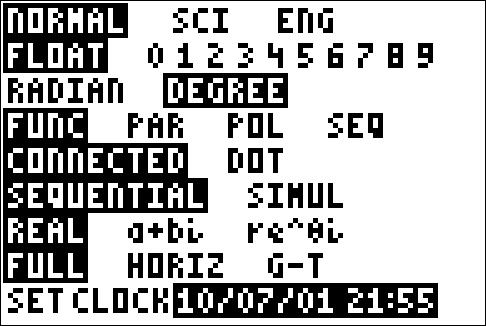
\includegraphics[width=2in]{./IntroTrigGraphics/UnitCircle01.jpg} &
\hspace{0.75in} 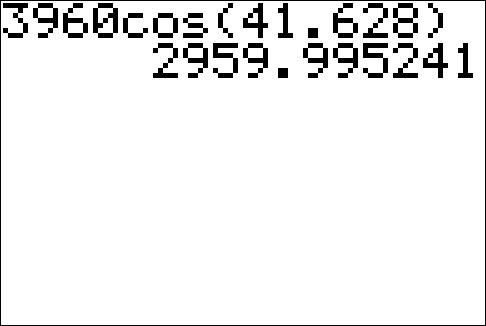
\includegraphics[width=2in]{./IntroTrigGraphics/UnitCircle02.jpg}  \\ 

\end{tabular} 

\end{center}

\vspace{-.35in} \qed

\end{enumerate}

\end{ex}

Theorem \ref{cosinesinecircle} gives us what we need to describe the position of an object traveling in a circular path of radius $r$ with constant angular velocity $\omega$.  Suppose that at time $t$, the object has swept out an angle measuring $\theta$ radians.  If we assume that the object is at the point $(r,0)$ when $t=0$, the angle $\theta$ is in standard position.  By definition, $\omega = \frac{\theta}{t}$ which we rewrite as  $\theta = \omega t$.  According to Theorem \ref{cosinesinecircle}, the location of the object $Q(x,y)$ on the circle is found using the equations  $x = r \cos(\theta) = r \cos(\omega t)$ and $y = r \sin(\theta) = r \sin(\omega t)$.  Hence, at time $t$, the object is at the point $(r \cos(\omega t), r \sin(\omega t))$.  We have just argued the following.


\smallskip

\colorbox{ResultColor}{\bbm
\begin{eqn} \label{equationsforcircularmotion} Suppose an object is traveling in a circular path of radius $r$ centered at the origin with constant angular velocity $\omega$.  If $t=0$ corresponds to the point $(r,0)$, then the $x$ and $y$ coordinates of the object are functions of $t$ and are given by $x =  r \cos(\omega t)$ and $y = r \sin(\omega t)$.  Here, $\omega > 0$ indicates a counter-clockwise direction and $\omega < 0$ indicates a clockwise direction.

\end{eqn}
\ebm}
\smallskip


\begin{center}

\hspace{.55in} \begin{mfpic}[15]{-5}{5}{-5}{5}
\axes
\tlabel(4.75,-0.5){\scriptsize $x$}
\tlabel(0.25,4.75){\scriptsize $y$}
\tlabel(2.1,-0.75){\scriptsize $1$}
\tlabel(0.25,2.1){\scriptsize $1$}
\tlabel(4.1,-0.75){\scriptsize $r$}
\tlabel(0.25,4.1){\scriptsize $r$}
\tlabel(2.35, 3.5){\small $Q\left(x,y\right) = (r \cos(\omega t), r \sin(\omega t))$}
\xmarks{-4 step 2 until 4}
\ymarks{-4 step 2 until 4}
\drawcolor[gray]{0.7}
\circle{(0,0),4}
\drawcolor[rgb]{0.33,0.33,0.33}
\arrow \polyline{(0,0), (2.5, 4.3301)}
\arrow \parafcn{5, 55, 5}{dir(t)}
\tlabel[cc](1.95, .5){\small $\theta = \omega t$}
\point[3pt]{(0,0),  (2, 3.4641)}
\penwd{1.5pt}
\arrow \parafcn{0, 60, 5}{4*dir(t)}
\end{mfpic} 

\hspace{-.7in} Equations for Circular Motion

\end{center}

\begin{ex}  Suppose we are in the situation of Example \ref{EarthRotationEx}.  Find the equations of motion of Lakeland Community College as the earth rotates.
\label{Lakelandrotates}

\smallskip

{\bf Solution.}  From Example \ref{EarthRotationEx}, we take $r = 2960$ miles and and $\omega = \frac{\pi}{12 \, \text{hours}}$.  Hence, the equations of motion are $x =  r \cos(\omega t) = 2960 \cos\left(\frac{\pi}{12} t\right)$ and  $y =  r \sin(\omega t) = 2960 \sin\left(\frac{\pi}{12} t\right)$, where $x$ and $y$ are measured in miles and $t$ is measured in hours. \qed

\end{ex}

In addition to circular motion, Theorem \ref{cosinesinecircle} is also the key to developing what is usually called `right triangle' trigonometry.\footnote{You may have been exposed to this in High School.}  As we shall see in the sections to come, many applications in trigonometry involve finding the measures of the angles in, and lengths of the sides of, right triangles.  Indeed, we made good use of some properties of right triangles to find the exact values of the cosine and sine of many of the angles in Example \ref{cosinesineviaunitcircle}, so the following development shouldn't be that much of a surprise.  Consider the generic right triangle below with corresponding acute angle $\theta$. The side with length $a$ is called the side of the triangle \emph{adjacent} to  $\theta$; the side with length $b$ is called the side of the triangle \emph{opposite} $\theta$; and the remaining side of length $c$ (the side opposite the right angle) is called the hypotenuse. We now imagine drawing this triangle in Quadrant I so that the angle $\theta$ is in standard position with the adjacent side to $\theta$ lying along the positive $x$-axis. 

\vspace{.1in}

\hspace{.5in} \begin{tabular}{m{2.5in}m{0.5in}m{2.5in}}

\begin{mfpic}[15]{-5}{5}{-5}{5}
\polyline{(-4.330,0), (4.330,0), (4.330,5), (-4.330,0)}
\arrow \reverse \arrow \shiftpath{(-4.330,0)} \parafcn{5, 25, 5}{3*dir(t)}
\tlabel(-1, 0.6){$\theta$}
\tlabel(0,-0.75){$a$}
\tlabel(4.75,2.25){$b$}
\tlabel(0,3){$c$}
\polyline{(3.93, 0), (3.93, 0.4), (4.33, 0.4)}
\end{mfpic}
&

&

\begin{mfpic}[15]{-5}{5}{-5}{5}
\axes
\tlabel(4.75,-0.5){\scriptsize $x$}
\tlabel(0.25,4.75){\scriptsize $y$}
\tlabel(4.1,-1){\scriptsize $c$}
\tlabel(0.25,4.1){\scriptsize $c$}
\xmarks{-4 step 4 until 4}
\ymarks{-4 step 4 until 4}
\tlabel(3.75,1.60){$P(a,b)$}
\drawcolor[gray]{0.7}
\circle{(0,0),4}
\drawcolor[rgb]{0.33,0.33,0.33}
\arrow \polyline{(0,0), (4.330,2.5)}
\arrow \parafcn{5, 25, 5}{1.5*dir(t)}
\tlabel(1.75, .25){\scriptsize $\theta$}
\point[3pt]{(0,0), (3.4641, 2)}
\polyline{(3.4641,2), (3.4641, 0)}
\polyline{(3.1641, 0), (3.1641, 0.3), (3.4641, 0.3)}
\end{mfpic} 

\end{tabular}

According to the Pythagorean Theorem, $a^2+b^2=c^2$, so that the point $P(a,b)$ lies on a circle of radius $c$.  Theorem \ref{cosinesinecircle} tells us that $\cos(\theta) = \frac{a}{c}$ and $\sin(\theta) = \frac{b}{c}$, so we have determined the cosine and sine of $\theta$ in terms of the lengths of the sides of the right triangle.  Thus we have the following theorem.
 
\smallskip

\colorbox{ResultColor}{\bbm

\begin{thm} \label{cosinesinetriangle}  Suppose $\theta$ is an acute angle residing in a right triangle.  If the length of the side adjacent to $\theta$ is $a$, the length of the side opposite $\theta$ is $b$, and the length of the hypotenuse is $c$, then $\cos(\theta) = \dfrac{a}{c}$ and $\sin(\theta) = \dfrac{b}{c}$.

\end{thm}

\ebm}

\smallskip

\begin{ex}  \label{righttriangleex} Find the measure of the missing angle and the lengths of the missing sides of:

\begin{center}

\begin{mfpic}[18]{-5}{5}{-5}{5}
\polyline{(-4.330,0), (4.330,0), (4.330,5), (-4.330,0)}
\arrow \reverse \arrow \shiftpath{(-4.330,0)} \parafcn{5, 25, 5}{3*dir(t)}
\tlabel(-1, 0.6){$30^{\circ}$}
\tlabel(0,-0.75){$7$}
\polyline{(3.93, 0), (3.93, 0.4), (4.33, 0.4)}
\end{mfpic}

\end{center}

{\bf Solution.}  The first and easiest task is to find the measure of the missing angle.  Since the sum of angles of a triangle is $180^{\circ}$, we know that the missing angle has measure $180^{\circ} - 30^{\circ} - 90^{\circ} = 60^{\circ}$.  We now proceed to find the lengths of the remaining two sides of the triangle.  Let $c$ denote the length of the hypotenuse of the triangle.  By Theorem \ref{cosinesinetriangle}, we have $\cos\left(30^{\circ}\right) = \frac{7}{c}$, or $c = \frac{7}{\cos\left(30^{\circ}\right)}$.  Since $\cos\left(30^{\circ}\right) = \frac{\sqrt{3}}{2}$, we have, after the usual fraction gymnastics, $c = \frac{14 \sqrt{3}}{3}$.  At this point, we have two ways to proceed to find the length of the side opposite the $30^{\circ}$ angle, which we'll denote $b$.  We know the length of the adjacent side is $7$ and the length of the hypotenuse is $\frac{14 \sqrt{3}}{3}$, so we could use the Pythagorean Theorem to find the missing side and solve  $(7)^2 + b^2 = \left( \frac{14 \sqrt{3}}{3} \right)^{2}$ for $b$.  Alternatively, we could use Theorem \ref{cosinesinetriangle}, namely that $\sin\left(30^{\circ}\right) = \frac{b}{c}$.  Choosing the latter, we find $b = c \sin\left(30^{\circ}\right) = \frac{14 \sqrt{3}}{3} \cdot \frac{1}{2} = \frac{7 \sqrt{3}}{3}$.  The triangle with all of its data is recorded below.

\begin{center}

\begin{mfpic}[18]{-5}{5}{-5}{5}
\polyline{(-4.330,0), (4.330,0), (4.330,5), (-4.330,0)}
\arrow \reverse \arrow \shiftpath{(-4.330,0)} \parafcn{5, 25, 5}{3*dir(t)}
\arrow \reverse \arrow \shiftpath{(4.330,5)}  \parafcn{215, 265, 5}{1.5*dir(t)}
\tlabel(-1, 0.6){$30^{\circ}$}
\tlabel(0,-0.75){$7$}
\tlabel(4.75,2.25){$b = \frac{7 \sqrt{3}}{3}$}
\tlabel(-2,3){$c = \frac{14 \sqrt{3}}{3}$}
\tlabel(2.75,2.9){$60^{\circ}$}
\polyline{(3.93, 0), (3.93, 0.4), (4.33, 0.4)}
\end{mfpic}

\end{center}

\vspace{-.45in} \qed

\end{ex}

\medskip

We close this section by noting that we can easily extend the functions cosine and sine to real numbers by identifying a real number $t$ with the angle $\theta = t$ radians.  Using this identification, we define $\cos(t) = \cos(\theta)$ and $\sin(t) = \sin(\theta)$. In practice this means expressions like $\cos(\pi)$ and $\sin(2)$ can be found by regarding the inputs as angles in radian measure or real numbers;  the choice is the reader's.  If we trace the identification of real numbers $t$ with angles $\theta$ in radian measure to its roots on page \pageref{wrappingfunction}, we can spell out this correspondence more precisely.  For each real number $t$, we associate an oriented arc $t$ units in length with initial point $(1,0)$ and endpoint $P(\cos(t), \sin(t))$.

\begin{tabular}{cc}

\begin{mfpic}[18]{-5}{5}{-4}{4.5}
\axes
\tlabel(4.75,-0.5){\scriptsize $x$}
\tlabel(0.25,4.25){\scriptsize $y$}
\tlabel(3.1,-0.75){\scriptsize $1$}
\tlabel(0.25,3.1){\scriptsize $1$}
\xmarks{-3 step 3 until 3}
\ymarks{-3 step 3 until 3}
\point[3pt]{(0,0)}
\drawcolor[gray]{0.7}
\circle{(0,0),3}
\drawcolor[rgb]{0.33,0.33,0.33}
\arrow \polyline{(0,0), (2.5, 4.3301)}
\arrow \reverse \arrow \polyline{(3,-4), (3,4.5)}
\polyline{(2.8,3.1416), (3.2,3.1416)}
\arrow \parafcn{5, 55, 5}{1.5*dir(t)}
\tlabel[cc](1.9, 1){$\theta = t$}
\penwd{1.5pt}
\arrow \polyline{(3,0), (3, 3.1416)}
\arrow \parafcn{0,60,5}{3*dir(t)}
\tlabel[cc](3.5,1.75){$t$}
\end{mfpic} 

&

\hspace{.3in}

\begin{mfpic}[18]{-5}{5}{-4}{4.5}
\axes
\tlabel(4.75,-0.5){\scriptsize $x$}
\tlabel(0.25,4.25){\scriptsize $y$}
\tlabel(3.1,-0.75){\scriptsize $1$}
\tlabel(0.25,3.1){\scriptsize $1$}
\xmarks{-3 step 3 until 3}
\ymarks{-3 step 3 until 3}
\arrow \polyline{(0,0), (2.5, 4.3301)}
\tlabel(2,2.6){$P(\cos(t), \sin(t))$}
\drawcolor[gray]{0.7}
\circle{(0,0),3}
\drawcolor[rgb]{0.33,0.33,0.33}
\arrow \parafcn{5, 55, 5}{1.5*dir(t)}
\tlabel[cc](1.9, 1){$\theta = t$}
\point[3pt]{(0,0), (1.5, 2.5981)}
\penwd{1.5pt}
\arrow \parafcn{0,60,5}{3*dir(t)}
\end{mfpic} 

\end{tabular}

In the same way we studied polynomial, rational, exponential, and logarithmic functions, we will study the trigonometric functions $f(t) = \cos(t)$ and $g(t) = \sin(t)$.  The first order of business is to find the domains and ranges of these functions.  Whether we think of identifying the real number $t$ with the angle $\theta = t$ radians, or think of wrapping an oriented arc around the Unit Circle to find coordinates on the Unit Circle, it should be clear that both the cosine and sine functions are defined for all real numbers $t$.  In other words, the domain  of $f(t) = \cos(t)$ and of $g(t) = \sin(t)$ is $(-\infty, \infty)$.  Since $\cos(t)$ and $\sin(t)$ represent $x$- and $y$-coordinates, respectively, of points on the Unit Circle, they both take on all of the values between $-1$ an $1$, inclusive.  In other words, the range of $f(t) = \cos(t)$ and of $g(t) = \sin(t)$ is the interval $[-1,1]$.  To summarize:

\smallskip

\colorbox{ResultColor}{\bbm

\begin{thm} \label{cosinesinefunctiondomainrange}  \textbf{Domain and Range of the Cosine and Sine Functions:} 

\vspace{.2in}

\begin{tabular}{ll}

\hspace{.3in} $\bullet \, $ The function $f(t) = \cos(t)$ & \hspace{.8in} $\bullet \, $ The function $g(t) = \sin(t)$ \\ [4pt]
\hspace{.5in} -- has domain $(-\infty, \infty)$ & \hspace{1in} -- has domain $(-\infty, \infty)$ \\ [4pt]
\hspace{.5in} -- has range $[-1,1]$ & \hspace{1in} -- has range $[-1,1]$ \\ [4pt]

\end{tabular}

\end{thm}

\ebm}

\smallskip
\phantomsection
\label{cosinesineequationsrealnumbers}

Suppose, as in the Exercises, we are asked to solve an equation such as $\sin(t) = -\frac{1}{2}$.  As we have already mentioned, the distinction between $t$ as a real number and as an angle $\theta = t$ radians is often blurred. Indeed, we solve $\sin(t) = -\frac{1}{2}$ in the exact same manner\footnote{Well, to be pedantic, we would be technically using `reference numbers' or `reference arcs' instead of `reference angles' -- but the idea is the same.} as we did in Example \ref{solveforangle} number \ref{sineisnegativehalf}.  Our solution is only cosmetically different in that the variable used is $t$ rather than $\theta$:  $t = \frac{7\pi}{6} + 2\pi k$ or  $t = \frac{11\pi}{6} + 2\pi k$ for integers, $k$.  We will study the cosine and sine functions in greater detail in Section \ref{TrigGraphs}.  Until then, keep in mind that any properties of cosine and sine developed in the following sections which regard them as functions of \textit{angles} in \textit{radian} measure apply equally well if the inputs are regarded as \textit{real numbers}.

\newpage

\subsection{Exercises}

In Exercises \ref{valuefirst} - \ref{valuelast}, find the exact value of the cosine and sine of the given angle.

\begin{multicols}{4}

\begin{enumerate}

\item $\theta = 0$ \vphantom{$\dfrac{\pi}{4}$} \label{valuefirst}
\item $\theta = \dfrac{\pi}{4}$
\item $\theta = \dfrac{\pi}{3}$
\item $\theta = \dfrac{\pi}{2}$

\setcounter{HW}{\value{enumi}}

\end{enumerate}

\end{multicols}

\begin{multicols}{4}

\begin{enumerate}

\setcounter{enumi}{\value{HW}}

\item $\theta = \dfrac{2\pi}{3}$
\item $\theta = \dfrac{3\pi}{4}$
\item $\theta = \pi$ \vphantom{$\dfrac{7\pi}{4}$}
\item $\theta = \dfrac{7\pi}{6}$

\setcounter{HW}{\value{enumi}}

\end{enumerate}

\end{multicols}

\begin{multicols}{4}

\begin{enumerate}

\setcounter{enumi}{\value{HW}}

\item $\theta = \dfrac{5\pi}{4}$
\item $\theta = \dfrac{4\pi}{3}$
\item $\theta = \dfrac{3\pi}{2}$
\item $\theta = \dfrac{5\pi}{3}$

\setcounter{HW}{\value{enumi}}

\end{enumerate}

\end{multicols}

\begin{multicols}{4}

\begin{enumerate}

\setcounter{enumi}{\value{HW}}

\item $\theta = \dfrac{7\pi}{4}$
\item $\theta = \dfrac{23\pi}{6}$
\item $\theta = -\dfrac{13\pi}{2}$
\item $\theta = -\dfrac{43\pi}{6}$

\setcounter{HW}{\value{enumi}}

\end{enumerate}

\end{multicols}

\begin{multicols}{4}

\begin{enumerate}

\setcounter{enumi}{\value{HW}}

\item $\theta = -\dfrac{3\pi}{4}$
\item $\theta = -\dfrac{\pi}{6}$ \vphantom{$\dfrac{7\pi}{4}$}
\item $\theta = \dfrac{10\pi}{3}$
\item $\theta = 117\pi$ \vphantom{$\dfrac{7\pi}{4}$} \label{valuelast}

\setcounter{HW}{\value{enumi}}

\end{enumerate}

\end{multicols}

In Exercises \ref{findthevaluefirst} - \ref{findthevaluelast}, use the results developed throughout the section to find the requested value.

\begin{enumerate}

\setcounter{enumi}{\value{HW}}

\item If $\sin(\theta) = -\dfrac{7}{25}$ with $\theta$ in Quadrant IV, what is $\cos(\theta)$? \label{findthevaluefirst}
\item If $\cos(\theta) = \dfrac{4}{9}$ with $\theta$ in Quadrant I, what is $\sin(\theta)$?
\item If $\sin(\theta) = \dfrac{5}{13}$ with $\theta$ in Quadrant II, what is $\cos(\theta)$?
\item If $\cos(\theta) = -\dfrac{2}{11}$ with $\theta$ in Quadrant III, what is $\sin(\theta)$?
\item If $\sin(\theta) = -\dfrac{2}{3}$ with $\theta$ in Quadrant III, what is $\cos(\theta)$?
\item If $\cos(\theta) = \dfrac{28}{53}$ with $\theta$ in Quadrant IV, what is $\sin(\theta)$?
\item  If $\sin(\theta) = \dfrac{2\sqrt{5}}{5}$ and $\dfrac{\pi}{2} < \theta < \pi$, what is $\cos(\theta)$?
\item  If $\cos(\theta) = \dfrac{\sqrt{10}}{10}$ and $2\pi < \theta < \dfrac{5\pi}{2}$, what is $\sin(\theta)$?
\item  If $\sin(\theta) = -0.42$ and $\pi < \theta < \dfrac{3\pi}{2}$, what is  $\cos(\theta)$?
\item  If $\cos(\theta) = -0.98$ and $\dfrac{\pi}{2} < \theta < \pi$, what is $\sin(\theta)$? \label{findthevaluelast}

\setcounter{HW}{\value{enumi}}

\end{enumerate}

\pagebreak

In Exercises \ref{solveforanglefirst} - \ref{solveforanglelast}, find all of the angles which satisfy the given equation.

\begin{multicols}{3}

\begin{enumerate}

\setcounter{enumi}{\value{HW}}

\item $\sin(\theta) = \dfrac{1}{2}$ \vphantom{$\dfrac{2}{2}$} \label{solveforanglefirst}
\item $\cos(\theta) = -\dfrac{\sqrt{3}}{2}$
\item $\sin(\theta) = 0$ \vphantom{$\dfrac{2}{2}$}

\setcounter{HW}{\value{enumi}}

\end{enumerate}

\end{multicols}

\begin{multicols}{3}

\begin{enumerate}

\setcounter{enumi}{\value{HW}}

\item $\cos(\theta) = \dfrac{\sqrt{2}}{2}$
\item $\sin(\theta) = \dfrac{\sqrt{3}}{2}$
\item $\cos(\theta) = -1$ \vphantom{$\dfrac{\sqrt{2}}{2}$}

\setcounter{HW}{\value{enumi}}

\end{enumerate}

\end{multicols}

\begin{multicols}{3}

\begin{enumerate}

\setcounter{enumi}{\value{HW}}

\item  $\sin(\theta) = -1$ \vphantom{$\dfrac{\sqrt{2}}{2}$}
\item  $\cos(\theta) = \dfrac{\sqrt{3}}{2}$
\item  $\cos(\theta) = -1.001$ \vphantom{$\dfrac{\sqrt{2}}{2}$} \label{solveforanglelast}

\setcounter{HW}{\value{enumi}}

\end{enumerate}

\end{multicols}

In Exercises \ref{solvefortfirst} - \ref{solvefortlast}, solve the equation for $t$.  (See the comments following Theorem \ref{cosinesinefunctiondomainrange}.)

\begin{multicols}{3}

\begin{enumerate}

\setcounter{enumi}{\value{HW}}

\item $\cos(t) = 0$ \vphantom{$\dfrac{\sqrt{2}}{2}$} \label{solvefortfirst}
\item $\sin(t) = -\dfrac{\sqrt{2}}{2}$
\item $\cos(t) = 3$ \vphantom{$\dfrac{\sqrt{2}}{2}$}

\setcounter{HW}{\value{enumi}}

\end{enumerate}

\end{multicols}

\begin{multicols}{3}

\begin{enumerate}

\setcounter{enumi}{\value{HW}}

\item $\sin(t) = -\dfrac{1}{2}$
\item $\cos(t) = \dfrac{1}{2}$
\item $\sin(t) = -2$ \vphantom{$\dfrac{1}{2}$}

\setcounter{HW}{\value{enumi}}

\end{enumerate}

\end{multicols}

\begin{multicols}{3}

\begin{enumerate}

\setcounter{enumi}{\value{HW}}

\item $\cos(t) = 1$ \vphantom{$\dfrac{\sqrt{2}}{2}$}
\item $\sin(t) = 1$ \vphantom{$\dfrac{\sqrt{2}}{2}$}
\item $\cos(t) = -\dfrac{\sqrt{2}}{2}$ \label{solvefortlast}

\setcounter{HW}{\value{enumi}}

\end{enumerate}

\end{multicols}

In Exercises \ref{calculatorfirst} - \ref{calculatorlast}, use your calculator to approximate the given value to three decimal places.  Make sure your calculator is in the proper angle measurement mode!

\begin{multicols}{3}

\begin{enumerate}

\setcounter{enumi}{\value{HW}}

\item $\sin(78.95^{\circ})$ \label{calculatorfirst}
\item $\cos(-2.01)$
\item $\sin(392.994)$

\setcounter{HW}{\value{enumi}}

\end{enumerate}

\end{multicols}

\begin{multicols}{3}

\begin{enumerate}

\setcounter{enumi}{\value{HW}}

\item $\cos(207^{\circ})$
\item $\sin\left( \pi^{\circ} \right)$
\item $\cos(e)$ \label{calculatorlast} 

\setcounter{HW}{\value{enumi}}

\end{enumerate}

\end{multicols}

In Exercises \ref{firsttriangle} - \ref{lasttriangle}, find the measurement of the missing angle and the lengths of the missing sides.  (See Example \ref{righttriangleex})

\begin{multicols}{2}

\begin{enumerate}

\setcounter{enumi}{\value{HW}}

\item Find $\theta$, $b$, and $c$. \label{firsttriangle}

 \begin{mfpic}[15]{-5}{5}{-5}{5}
\polyline{(-4.330,0), (4.330,0), (4.330,5), (-4.330,0)}
\arrow \reverse \arrow \shiftpath{(-4.330,0)} \parafcn{5, 25, 5}{3*dir(t)}
\arrow \reverse \arrow \shiftpath{(4.330,5)}  \parafcn{215, 265, 5}{1.5*dir(t)}
\tlabel(-1, 0.6){$30^{\circ}$}
\tlabel(0,-0.75){$1$}
\tlabel(4.75,2.25){$b$}
\tlabel(-0.5,3){$c$}
\tlabel(3,3){$\theta$}
\polyline{(3.93, 0), (3.93, 0.4), (4.33, 0.4)}
\end{mfpic}

\item  Find $\theta$, $a$, and $c$.

\begin{mfpic}[18]{-5}{5}{-5}{5}
\polyline{(-2.5, 0), (2.5,0), (-2.5,5), (-2.5,0)}
\arrow \reverse \arrow \shiftpath{(2.5,0)} \parafcn{140, 175, 5}{1.5*dir(t)}
\arrow \reverse \arrow \shiftpath{(-2.5,5)}  \parafcn{275, 310, 5}{1.5*dir(t)}
\tlabel(-2, 2.75){$45^{\circ}$}
\tlabel(-0.5,-0.75){$3$}
\tlabel(-3.25,2.25){$a$}
\tlabel(0,3){$c$}
\tlabel(0.5,0.5){$\theta$}
\polyline{(-2.5, 0.4), (-2.1, 0.4), (-2.1, 0)}
\end{mfpic}

\setcounter{HW}{\value{enumi}}

\end{enumerate}

\end{multicols}

\pagebreak

\begin{multicols}{2}

\begin{enumerate}

\setcounter{enumi}{\value{HW}}

\item  Find $\alpha$, $a$, and $b$.

\begin{mfpic}[18]{-1}{5}{-1}{7}
\polyline{(0,0), (0,6.709), (4.357, 6.709), (0,0)}
\arrow \reverse \arrow \parafcn{60, 87, 5}{1.75*dir(t)}
\arrow \reverse \arrow \shiftpath{(4.357,6.709)}  \parafcn{185, 232, 5}{1.5*dir(t)}
\tlabel(0.25, 2){$33^{\circ}$}
\tlabel(3,3){$8$}
\tlabel(2,7){$b$}
\tlabel(-0.75,4){$a$}
\tlabel(2.25,5.75){$\alpha$}
\polyline{(0,6.304), (0.4, 6.304),  (0.4, 6.704)}
\end{mfpic}

\item Find $\beta$, $a$, and $c$. \label{lasttriangle}

\begin{mfpic}[18]{-6}{1}{-1}{9}
\polyline{(0,0), (0,6), (-5.402, 6), (0,0)}
\arrow \reverse \arrow \parafcn{95, 127, 5}{1.75*dir(t)}
\arrow \reverse \arrow \shiftpath{(-5.402,6)}  \parafcn{317, 355, 5}{1.5*dir(t)}
\tlabel(-3.75, 5){$48^{\circ}$}
\tlabel(0.5,3){$6$}
\tlabel(-2.6,6.25){$a$}
\tlabel(-3.25,2.5){$c$}
\tlabel(-1,2){$\beta$}
\polyline{(0,5.6), (-0.4, 5.6),  (-0.4, 6)}
\end{mfpic} 

\setcounter{HW}{\value{enumi}}

\end{enumerate}

\end{multicols}

In Exercises \ref{missingsidefirst} - \ref{missingsidelast}, assume that $\theta$ is an acute angle in a right triangle and use Theorem \ref{cosinesinetriangle} to find the requested side.

\begin{enumerate}

\setcounter{enumi}{\value{HW}}

\item If $\theta = 12^{\circ}$ and the side adjacent to $\theta$ has length 4, how long is the hypotenuse? \label{missingsidefirst}
\item If $\theta = 78.123^{\circ}$ and the hypotenuse has length 5280, how long is the side adjacent to $\theta$?
\item If $\theta = 59^{\circ}$ and the side opposite $\theta$ has length 117.42, how long is the hypotenuse?
\item If $\theta = 5^{\circ}$ and the hypotenuse has length 10, how long is the side opposite $\theta$?
\item If $\theta = 5^{\circ}$ and the hypotenuse has length 10, how long is the side adjacent to $\theta$?
\item If $\theta = 37.5^{\circ}$ and the side opposite $\theta$ has length 306, how long is the side adjacent to $\theta$? \label{missingsidelast}

\setcounter{HW}{\value{enumi}}

\end{enumerate}

In Exercises \ref{pointsfirst} - \ref{pointslast}, let $\theta$ be the angle in standard position whose terminal side contains the given point then compute $\cos(\theta)$ and $\sin(\theta)$.

\begin{multicols}{4}

\begin{enumerate}

\setcounter{enumi}{\value{HW}}

\item $P(-7, 24)$ \label{pointsfirst} 
\item $Q(3, 4)$
\item $R(5, -9)$
\item $T(-2, -11)$ \label{pointslast}

\setcounter{HW}{\value{enumi}}

\end{enumerate}

\end{multicols}

In Exercises \ref{motionfirst} - \ref{motionlast}, find the equations of motion for the given scenario.  Assume that the center of the motion is the origin, the motion is counter-clockwise and that $t = 0$ corresponds to a position along the positive $x$-axis.  (See Equation \ref{equationsforcircularmotion} and Example \ref{EarthRotationEx}.)

\begin{enumerate}

\setcounter{enumi}{\value{HW}}

\item  \label{motionfirst} A point on the edge of the spinning yo-yo in Exercise \ref{spinningyoyo} from Section \ref{Angles}. 

Recall: The diameter of the yo-yo is 2.25 inches and it spins at 4500 revolutions per minute.

\item  The yo-yo in exercise \ref{yoyotrick} from Section \ref{Angles}.

Recall: The radius of the circle is 28 inches and it completes one revolution in 3 seconds.

\item A point on the edge of the hard drive in Exercise \ref{harddrive} from Section \ref{Angles}.

Recall:  The diameter of the hard disk is 2.5 inches and it spins at 7200 revolutions per minute.

\item  \label{motionlast} A passenger on the Big Wheel in Exercise \ref{giantwheelmotion} from Section \ref{Angles}.

Recall: The diameter is 128 feet and completes 2 revolutions in 2 minutes, 7 seconds.

\setcounter{HW}{\value{enumi}}

\end{enumerate}

\begin{enumerate}

\setcounter{enumi}{\value{HW}}

\item Consider the numbers:  $0$, $1$, $2$, $3$, $4$.  Take the square root of each of these numbers, then divide each by $2$. The resulting numbers should look hauntingly familiar. (See the values in the table on \pageref{CosineSineFacts}.) 

\item Let $\alpha$ and $\beta$ be the two acute angles of a right triangle.  (Thus $\alpha$ and $\beta$ are complementary angles.)  Show that $\sin(\alpha) = \cos(\beta)$ and $\sin(\beta) = \cos(\alpha)$.  The fact that co-functions of complementary angles are equal in this case is not an accident and a more general result will be given in Section \ref{Identities}.
\label{cofunctionforeshadowing}

\item  In the scenario of Equation \ref{equationsforcircularmotion}, we assumed that at $t=0$, the object was at the point $(r,0)$.  If this is not the case,  we can adjust the equations of motion by introducing a `time delay.'   If $t_{0} > 0$ is the first time the object passes through the point $(r,0)$, show, with the help of your classmates, the equations of motion are $x = r \cos(\omega (t - t_{0}))$ and $y = r \sin(\omega (t-t_{0}))$.

\end{enumerate}

\newpage

\subsection{Answers}

\begin{multicols}{2}

\begin{enumerate}

\item $\cos(0) = 1$, $\; \sin(0) = 0$ \vphantom{$\dfrac{\sqrt{2}}{2}$}

\item $\cos \left(\dfrac{\pi}{4} \right) = \dfrac{\sqrt{2}}{2}$, $\; \sin \left(\dfrac{\pi}{4} \right) = \dfrac{\sqrt{2}}{2}$

\setcounter{HW}{\value{enumi}}

\end{enumerate}

\end{multicols}

\begin{multicols}{2}

\begin{enumerate}

\setcounter{enumi}{\value{HW}}

\item $\cos \left(\dfrac{\pi}{3}\right) = \dfrac{1}{2}$, $\; \sin \left(\dfrac{\pi}{3}\right) = \dfrac{\sqrt{3}}{2}$

\item $\cos \left(\dfrac{\pi}{2}\right) = 0$, $\; \sin \left(\dfrac{\pi}{2}\right) = 1$ \vphantom{$\dfrac{\sqrt{2}}{2}$}

\setcounter{HW}{\value{enumi}}

\end{enumerate}

\end{multicols}

\begin{multicols}{2}

\begin{enumerate}

\setcounter{enumi}{\value{HW}}

\item $\cos\left(\dfrac{2\pi}{3}\right) = -\dfrac{1}{2}$, $\; \sin \left(\dfrac{2\pi}{3}\right) = \dfrac{\sqrt{3}}{2}$

\item $\cos \left(\dfrac{3\pi}{4} \right) = -\dfrac{\sqrt{2}}{2}$, $\; \sin \left(\dfrac{3\pi}{4} \right) = \dfrac{\sqrt{2}}{2}$

\setcounter{HW}{\value{enumi}}

\end{enumerate}

\end{multicols}

\begin{multicols}{2}

\begin{enumerate}

\setcounter{enumi}{\value{HW}}

\item $\cos(\pi) = -1$, $\; \sin(\pi) = 0$ \vphantom{$\dfrac{\sqrt{3}}{2}$}

\item $\cos\left(\dfrac{7\pi}{6}\right) = -\dfrac{\sqrt{3}}{2}$, $\; \sin\left(\dfrac{7\pi}{6}\right) = -\dfrac{1}{2}$

\setcounter{HW}{\value{enumi}}

\end{enumerate}

\end{multicols}

\begin{multicols}{2}

\begin{enumerate}

\setcounter{enumi}{\value{HW}}

\item $\cos \left(\dfrac{5\pi}{4} \right) = -\dfrac{\sqrt{2}}{2}$, $\; \sin \left(\dfrac{5\pi}{4} \right) = -\dfrac{\sqrt{2}}{2}$

\item $\cos\left(\dfrac{4\pi}{3}\right) = -\dfrac{1}{2}$, $\; \sin \left(\dfrac{4\pi}{3}\right) = -\dfrac{\sqrt{3}}{2}$

\setcounter{HW}{\value{enumi}}

\end{enumerate}

\end{multicols}

\begin{multicols}{2}

\begin{enumerate}

\setcounter{enumi}{\value{HW}}

\item $\cos \left(\dfrac{3\pi}{2}\right) = 0$, $\; \sin \left(\dfrac{3\pi}{2}\right) = -1$

\item $\cos\left(\dfrac{5\pi}{3}\right) = \dfrac{1}{2}$, $\; \sin \left(\dfrac{5\pi}{3}\right) = -\dfrac{\sqrt{3}}{2}$

\setcounter{HW}{\value{enumi}}

\end{enumerate}

\end{multicols}

\begin{multicols}{2}

\begin{enumerate}

\setcounter{enumi}{\value{HW}}

\item $\cos \left(\dfrac{7\pi}{4} \right) = \dfrac{\sqrt{2}}{2}$, $\; \sin \left(\dfrac{7\pi}{4} \right) = -\dfrac{\sqrt{2}}{2}$

\item $\cos\left(\dfrac{23\pi}{6}\right) = \dfrac{\sqrt{3}}{2}$, $\; \sin\left(\dfrac{23\pi}{6}\right) = -\dfrac{1}{2}$

\setcounter{HW}{\value{enumi}}

\end{enumerate}

\end{multicols}

\begin{multicols}{2}

\begin{enumerate}

\setcounter{enumi}{\value{HW}}

\item $\cos \left(-\dfrac{13\pi}{2}\right) = 0$, $\; \sin \left(-\dfrac{13\pi}{2}\right) = -1$ \vphantom{$\dfrac{\sqrt{3}}{2}$}

\item $\cos\left(-\dfrac{43\pi}{6}\right) = -\dfrac{\sqrt{3}}{2}$, $\; \sin\left(-\dfrac{43\pi}{6}\right) = \dfrac{1}{2}$

\setcounter{HW}{\value{enumi}}

\end{enumerate}

\end{multicols}

\begin{multicols}{2}

\begin{enumerate}

\setcounter{enumi}{\value{HW}}

\item $\cos \left(-\dfrac{3\pi}{4} \right) = -\dfrac{\sqrt{2}}{2}$, $\; \sin \left(-\dfrac{3\pi}{4} \right) = -\dfrac{\sqrt{2}}{2}$

\item $\cos\left(-\dfrac{\pi}{6}\right) = \dfrac{\sqrt{3}}{2}$, $\; \sin\left(-\dfrac{\pi}{6}\right) = -\dfrac{1}{2}$

\setcounter{HW}{\value{enumi}}

\end{enumerate}

\end{multicols}

\begin{multicols}{2}

\begin{enumerate}

\setcounter{enumi}{\value{HW}}

\item $\cos\left(\dfrac{10\pi}{3}\right) = -\dfrac{1}{2}$, $\; \sin \left(\dfrac{10\pi}{3}\right) = -\dfrac{\sqrt{3}}{2}$

\item $\cos(117\pi) = -1$, $\; \sin(117\pi) = 0$ \vphantom{$\dfrac{\sqrt{3}}{2}$}

\setcounter{HW}{\value{enumi}}

\end{enumerate}

\end{multicols}

\begin{enumerate}

\setcounter{enumi}{\value{HW}}

\item If $\sin(\theta) = -\dfrac{7}{25}$ with $\theta$ in Quadrant IV, then $\cos(\theta) = \dfrac{24}{25}$.
\item If $\cos(\theta) = \dfrac{4}{9}$ with $\theta$ in Quadrant I, then $\sin(\theta) = \dfrac{\sqrt{65}}{9}$.
\item If $\sin(\theta) = \dfrac{5}{13}$ with $\theta$ in Quadrant II, then $\cos(\theta) = -\dfrac{12}{13}$.
\item If $\cos(\theta) = -\dfrac{2}{11}$ with $\theta$ in Quadrant III, then $\sin(\theta) = -\dfrac{\sqrt{117}}{11}$.
\item If $\sin(\theta) = -\dfrac{2}{3}$ with $\theta$ in Quadrant III, then $\cos(\theta) = -\dfrac{\sqrt{5}}{3}$.
\item If $\cos(\theta) = \dfrac{28}{53}$ with $\theta$ in Quadrant IV, then $\sin(\theta) = -\dfrac{45}{53}$.
\item  If $\sin(\theta) = \dfrac{2\sqrt{5}}{5}$ and $\dfrac{\pi}{2} < \theta < \pi$, then $\cos(\theta) = -\dfrac{\sqrt{5}}{5}$.
\item  If $\cos(\theta) = \dfrac{\sqrt{10}}{10}$ and $2\pi < \theta < \dfrac{5\pi}{2}$, then $\sin(\theta)  = \dfrac{3 \sqrt{10}}{10}$.
\item  If $\sin(\theta) = -0.42$ and $\pi < \theta < \dfrac{3\pi}{2}$, then $\cos(\theta) = -\sqrt{0.8236} \approx -0.9075$.
\item  If $\cos(\theta) = -0.98$ and $\dfrac{\pi}{2} < \theta < \pi$, then $\sin(\theta) = \sqrt{0.0396} \approx 0.1990$.

\setcounter{HW}{\value{enumi}}

\end{enumerate}

\begin{enumerate}

\setcounter{enumi}{\value{HW}}

\item $\sin(\theta) = \dfrac{1}{2}$ when $\theta = \dfrac{\pi}{6} + 2\pi k$ or $\theta = \dfrac{5\pi}{6} + 2\pi k$ for any integer $k$.
\item $\cos(\theta) = -\dfrac{\sqrt{3}}{2}$ when $\theta = \dfrac{5\pi}{6} + 2\pi k$ or $\theta = \dfrac{7\pi}{6} + 2\pi k$ for any integer $k$.
\item $\sin(\theta) = 0$ when $\theta = \pi k$ for any integer $k$.
\item $\cos(\theta) = \dfrac{\sqrt{2}}{2}$ when $\theta = \dfrac{\pi}{4} + 2\pi k$ or $\theta = \dfrac{7\pi}{4} + 2\pi k$ for any integer $k$.
\item $\sin(\theta) = \dfrac{\sqrt{3}}{2}$ when $\theta = \dfrac{\pi}{3} + 2\pi k$ or $\theta = \dfrac{2\pi}{3} + 2\pi k$ for any integer $k$.
\item $\cos(\theta) = -1$ when $\theta = (2k + 1)\pi$ for any integer $k$.
\item  $\sin(\theta) = -1$ when $\theta = \dfrac{3\pi}{2} + 2\pi k$ for any integer $k$.
\item  $\cos(\theta) = \dfrac{\sqrt{3}}{2}$ when $\theta = \dfrac{\pi}{6} + 2\pi k$ or  $\theta = \dfrac{11\pi}{6} + 2\pi k$ for any integer $k$.
%\item  $\sin(\theta) = \dfrac{\sqrt{2}}{2}$ when $\theta = \dfrac{\pi}{4} + 2\pi k$ or  $\theta = \dfrac{3\pi}{4} + 2\pi k$ for any integer $k$.
\item  $\cos(\theta) = -1.001$ never happens

\setcounter{HW}{\value{enumi}}

\end{enumerate}

\begin{enumerate}

\setcounter{enumi}{\value{HW}}

\item $\cos(t) = 0$ when $t = \dfrac{\pi}{2} + \pi k$ for any integer $k$.
\item $\sin(t) = -\dfrac{\sqrt{2}}{2}$ when $t = \dfrac{5\pi}{4} + 2\pi k$ or $t = \dfrac{7\pi}{4} + 2\pi k$ for any integer $k$.
\item $\cos(t) = 3$ never happens.  
\item $\sin(t) = -\dfrac{1}{2}$ when $t = \dfrac{7\pi}{6} + 2\pi k$ or $t = \dfrac{11\pi}{6} + 2\pi k$ for any integer $k$.
\item $\cos(t) = \dfrac{1}{2}$ when $t = \dfrac{\pi}{3} + 2\pi k$ or $t = \dfrac{5\pi}{3} + 2\pi k$ for any integer $k$.
\item $\sin(t) = -2$ never happens
\item $\cos(t) = 1$ when $t = 2\pi k$ for any integer $k$.
\item $\sin(t) = 1$ when $t = \dfrac{\pi}{2} + 2\pi k$ for any integer $k$.
\item $\cos(t) = -\dfrac{\sqrt{2}}{2}$ when $t = \dfrac{3\pi}{4} + 2\pi k$ or $t = \dfrac{5\pi}{4} + 2\pi k$ for any integer $k$.
%\item  $\sin(t) = -\dfrac{\sqrt{3}}{2}$ when $t = \dfrac{4\pi}{3} + 2\pi k$ or  $t = \dfrac{5\pi}{3} + 2\pi k$ for any integer $k$.

\setcounter{HW}{\value{enumi}}

\end{enumerate}

\begin{multicols}{3}

\begin{enumerate}

\setcounter{enumi}{\value{HW}}

\item $\sin(78.95^{\circ}) \approx 0.981$
\item $\cos(-2.01) \approx -0.425$
\item $\sin(392.994) \approx -0.291$

\setcounter{HW}{\value{enumi}}

\end{enumerate}

\end{multicols}

\begin{multicols}{3}

\begin{enumerate}

\setcounter{enumi}{\value{HW}}

\item $\cos(207^{\circ}) \approx -0.891$
\item $\sin\left( \pi^{\circ} \right) \approx 0.055$
\item $\cos(e) \approx -0.912$

\setcounter{HW}{\value{enumi}}

\end{enumerate}

\end{multicols}

\begin{enumerate}

\setcounter{enumi}{\value{HW}}

\item $\theta = 60^{\circ}$, $b = \dfrac{ \sqrt{3}}{3}$, $c=\dfrac{2 \sqrt{3}}{3}$

\item  $\theta = 45^{\circ}$, $a = 3$, $c = 3\sqrt{2}$

\item  $\alpha = 57^{\circ}$, $a = 8 \cos(33^{\circ}) \approx 6.709$, $b = 8 \sin(33^{\circ}) \approx 4.357$

\item  $\beta = 42^{\circ}$, $c = \dfrac{6}{\sin(48^{\circ})} \approx 8.074$, $a = \sqrt{c^2 - 6^2} \approx 5.402$

\setcounter{HW}{\value{enumi}}

\end{enumerate}


\begin{enumerate}

\setcounter{enumi}{\value{HW}}

\item The hypotenuse has length $\dfrac{4}{\cos(12^{\circ})}\approx 4.089$.
\item The side adjacent to $\theta$ has length $5280\cos(78.123^{\circ}) \approx 1086.68$.
\item The hypotenuse has length $\dfrac{117.42}{\sin(59^{\circ})}\approx 136.99$.
\item The side opposite $\theta$ has length $10\sin(5^{\circ}) \approx 0.872$.
\item The side adjacent to $\theta$ has length $10\cos(5^{\circ}) \approx 9.962$.
\item The hypotenuse has length $c = \dfrac{306}{\sin(37.5^{\circ})}\approx 502.660$, so the side adjacent to $\theta$ has length  $\sqrt{c^2 - 306^{2}} \approx 398.797$.

\setcounter{HW}{\value{enumi}}

\end{enumerate}

\begin{enumerate}

\setcounter{enumi}{\value{HW}}

\item $\cos(\theta) = -\dfrac{7}{25}, \; \sin(\theta) = \dfrac{24}{25}$

\item $\cos(\theta) = \dfrac{3}{5}, \; \sin(\theta) = \dfrac{4}{5}$

\item $\cos(\theta) = \dfrac{5\sqrt{106}}{106}, \; \sin(\theta) = -\dfrac{9\sqrt{106}}{106}$

\item $\cos(\theta) = -\dfrac{2\sqrt{5}}{25}, \; \sin(\theta) = -\dfrac{11\sqrt{5}}{25}$

\setcounter{HW}{\value{enumi}}

\end{enumerate}

\begin{enumerate}

\setcounter{enumi}{\value{HW}}

\item   $r = 1.125$ inches, $\omega = 9000 \pi \, \frac{\text{radians}}{\text{minute}}$,  $x = 1.125 \cos(9000 \pi \, t)$, $y = 1.125 \sin(9000 \pi \, t)$.  Here $x$ and $y$ are measured in inches and $t$ is measured in minutes.

\item   $r = 28$ inches, $\omega = \frac{2\pi}{3} \, \frac{\text{radians}}{\text{second}}$,  $x = 28 \cos\left(\frac{2\pi}{3} \, t \right)$, $y = 28 \sin\left(\frac{2\pi}{3} \, t \right)$.  Here $x$ and $y$ are measured in inches and $t$ is measured in seconds.

\item $r = 1.25$ inches, $\omega = 14400 \pi \, \frac{\text{radians}}{\text{minute}}$,  $x = 1.25 \cos(14400 \pi \, t)$, $y = 1.25 \sin(14400 \pi \, t)$.  Here $x$ and $y$ are measured in inches and $t$ is measured in minutes.

\item  $r = 64$ feet, $\omega = \frac{4\pi}{127} \, \frac{\text{radians}}{\text{second}}$,  $x = 64 \cos\left(\frac{4\pi}{127} \, t \right)$, $y = 64 \sin\left(\frac{4\pi}{127} \, t \right)$.  Here $x$ and $y$ are measured in feet and $t$ is measured in seconds

\end{enumerate}


\closegraphsfile

\newpage

\section{The Six Circular Functions and Fundamental Identities}

\mfpicnumber{1}

\opengraphsfile{CircularFunctions}

\setcounter{footnote}{0}

\label{CircularFunctions}

In section \ref{TheUnitCircle},  we defined $\cos(\theta)$ and $\sin(\theta)$  for angles $\theta$ using the coordinate values of points on the Unit Circle.  As such, these functions earn the moniker \index{circular function}\index{function ! circular}\textbf{circular functions}.\footnote{In Theorem \ref{cosinesinetriangle} we also showed cosine and sine to be functions of an angle residing in a right triangle so we could just as easily call them \emph{trigonometric} functions.  In later sections, you will find that we do indeed use the phrase `trigonometric function' interchangeably with the term `circular function'.} It turns out that cosine and sine are just two of the six commonly used circular functions which we define below. 

\enlargethispage{.2in}

%\medskip

\colorbox{ResultColor}{\bbm

\begin{defn} \label{circularfunctions}  \textbf{The Circular Functions:} Suppose $\theta$ is an angle plotted in standard position and $P(x,y)$ is the point on the terminal side of $\theta$ which lies on the Unit Circle.  

\begin{itemize}

\item The \index{cosine ! of an angle} \textbf{cosine} of $\theta$, denoted $\cos(\theta)$, is defined by $\cos(\theta) = x$.

\item The \index{sine ! of an angle} \textbf{sine} of $\theta$, denoted $\sin(\theta)$, is defined by $\sin(\theta) = y$.

\item The \index{secant ! of an angle} \textbf{secant} of $\theta$, denoted $\sec(\theta)$, is defined by $\sec(\theta) = \dfrac{1}{x}$, provided $x \neq 0$.

\item The \index{cosecant ! of an angle} \textbf{cosecant} of $\theta$, denoted $\csc(\theta)$, is defined by $\csc(\theta) = \dfrac{1}{y}$, provided $y \neq 0$.

\item The \index{tangent ! of an angle} \textbf{tangent} of $\theta$, denoted $\tan(\theta)$, is defined by $\tan(\theta) = \dfrac{y}{x}$, provided $x \neq 0$.

\item The \index{cotangent ! of an angle} \textbf{cotangent} of $\theta$, denoted $\cot(\theta)$, is defined by $\cot(\theta) = \dfrac{x}{y}$, provided $y \neq 0$.

\end{itemize}

\end{defn}

\ebm}

\vspace{0.1in}

While we left the history of the name `sine' as an interesting research project in Section \ref{TheUnitCircle}, the names `tangent' and `secant' can be explained using the diagram below.  Consider the acute angle $\theta$ below in standard position. Let $P(x,y)$ denote, as usual,  the point on the terminal side of $\theta$ which lies on the Unit Circle and let $Q(1,y')$ denote the point on the terminal side of $\theta$ which lies on the vertical line $x=1$. 

\vspace{-0.1in}
\begin{center}

\begin{mfpic}[25]{-1}{7}{-1}{7}
\axes
\drawcolor[gray]{0.7}
\parafcn{0,90,5}{3*dir(t)}
\drawcolor[rgb]{0.33,0.33,0.33}
\arrow \parafcn{5, 55, 5}{0.75*dir(t)}
\tlabel[cc](0.75,0.5){\scriptsize $\theta$}
\point[3pt]{(0,0), (1.5, 2.5981), (3,5.196), (3,0), (1.5,0)}
\tlabel(6.75,-0.5){\scriptsize $x$}
\tlabel(0.25,6.75){\scriptsize $y$}
\tlabel(0.25,3.1){\scriptsize $1$}
\tlabel(-0.5,-0.5){\scriptsize $O$}
\tlabel(2.75,-0.5){\scriptsize $B(1,0)$}
\tlabel(1.25, -0.5){\scriptsize $A(x, 0)$}
\xmarks{0 step 3 until 3}
\ymarks{0 step 3 until 3}
\arrow \polyline{(0,0), (4,6.9282)}
\polyline{(3,0), (3,5.196)}
\polyline{(2.75,0), (2.75, 0.25), (3,0.25)}
\polyline{(1.5,0), (1.5, 2.5981)}
\polyline{(1.25,0), (1.25,0.25), (1.5,0.25)}
\tlabel(1.75,2.6){\scriptsize $P(x,y)$}
\tlabel(3.25,5.25){\scriptsize $Q(1,y') = (1, \tan(\theta))$}
\end{mfpic} 

\end{center}

%\medskip

The word `tangent' comes from the Latin meaning `to touch,' and for this reason, the line $x=1$ is called a \textit{tangent} line to the Unit Circle since it intersects, or `touches', the circle at only one point, namely $(1,0)$.  Dropping perpendiculars from $P$ and $Q$ creates a pair of similar triangles $\Delta OPA$ and $\Delta OQB$.  Thus $\frac{y'}{y} = \frac{1}{x}$ which gives  $y' = \frac{y}{x} = \tan(\theta)$, where this last equality comes from applying Definition  \ref{circularfunctions}. We have just shown that for acute angles $\theta$, $\tan(\theta)$ is the $y$-coordinate of the point on the terminal side of $\theta$ which lies on the line $x = 1$ which is \textit{tangent} to the Unit Circle. Now the word `secant' means `to cut', so a secant line is any line that `cuts through' a circle at two points.\footnote{Compare this with the definition given in Section \ref{LinearFunctions}.}  The line containing the terminal side of $\theta$ is a secant line since it intersects the Unit Circle in Quadrants I and III.   With the point $P$ lying on the Unit Circle, the length of the hypotenuse of $\Delta OPA$ is $1$. If we let $h$ denote the length of the hypotenuse of $\Delta OQB$, we have from similar triangles that $\frac{h}{1} = \frac{1}{x}$, or $h = \frac{1}{x} = \sec(\theta)$.  Hence for an acute angle $\theta$, $\sec(\theta)$ is the length of the line segment which lies on the secant line determined by the terminal side of $\theta$ and `cuts off' the tangent line $x=1$.  Not only do these observations help explain the names of these functions, they serve as the basis for a fundamental inequality needed for Calculus which we'll explore in the Exercises.

\smallskip 

Of the six circular functions, only cosine and sine are defined for all angles.  Since $\cos(\theta) = x$ and $\sin(\theta) = y$ in Definition \ref{circularfunctions}, it is customary to rephrase the remaining four circular functions in terms of cosine and sine.  The following theorem is a result of simply replacing $x$ with $\cos(\theta)$ and $y$ with $\sin(\theta)$ in Definition \ref{circularfunctions}.

\smallskip

\colorbox{ResultColor}{\bbm

\begin{thm} \label{recipquotid}  \textbf{Reciprocal and Quotient Identities:} \index{Reciprocal Identities} \index{Quotient Identities} 

\begin{itemize}

\item $\sec(\theta) = \dfrac{1}{\cos(\theta)}$, provided $\cos(\theta) \neq 0$;  if $\cos(\theta) = 0$, $\sec(\theta)$ is undefined.

\item $\csc(\theta) = \dfrac{1}{\sin(\theta)}$, provided $\sin(\theta) \neq 0$;  if $\sin(\theta) = 0$, $\csc(\theta)$ is undefined.

\item $\tan(\theta) = \dfrac{\sin(\theta)}{\cos(\theta)}$, provided $\cos(\theta) \neq 0$;  if $\cos(\theta) = 0$, $\tan(\theta)$ is undefined.

\item $\cot(\theta) = \dfrac{\cos(\theta)}{\sin(\theta)}$, provided $\sin(\theta) \neq 0$;  if $\sin(\theta) = 0$, $\cot(\theta)$ is undefined.

\end{itemize}

\end{thm}

\ebm}

\medskip

It is high time for an example.

\begin{ex} \label{circularfunctionsex}  Find the indicated value, if it exists.

\begin{multicols}{3}

\begin{enumerate}

\item  $\sec\left(60^{\circ}\right)$

\item  $\csc\left(\frac{7 \pi}{4} \right)$

\item  $\cot(3)$

\setcounter{HW}{\value{enumi}}

\end{enumerate}

\end{multicols}

\begin{enumerate}

\setcounter{enumi}{\value{HW}}

\item $\tan\left(\theta\right)$, where $\theta$ is any angle coterminal with $\frac{3\pi}{2}$.

\item $\cos\left(\theta\right)$, where $\csc(\theta) = -\sqrt{5}$ and $\theta$ is a Quadrant IV angle.

\item $\sin\left(\theta\right)$, where $\tan(\theta) = 3$ and $\pi < \theta < \frac{3\pi}{2}$.

\end{enumerate}

{\bf Solution.}  

\begin{enumerate}

\item  According to Theorem \ref{recipquotid},   $\sec\left(60^{\circ}\right) = \frac{1}{\cos\left(60^{\circ}\right)}$. Hence,  $\sec\left(60^{\circ}\right) = \frac{1}{(1/2)} = 2$.

\item  Since $\sin\left( \frac{7\pi}{4}\right) = - \frac{\sqrt{2}}{2}$,  $\csc\left( \frac{7\pi}{4}\right) = \frac{1}{\sin\left( \frac{7\pi}{4}\right)} = \frac{1}{- \sqrt{2}/2} = - \frac{2}{\sqrt{2}} = - \sqrt{2}$.

\item  Since $\theta = 3$ radians is not one of the `common angles' from Section \ref{TheUnitCircle}, we resort to the calculator for a decimal approximation.  Ensuring that the calculator is in radian mode, we find $\cot(3) = \frac{\cos(3)}{\sin(3)} \approx -7.015$.

\begin{tabular}{cc}

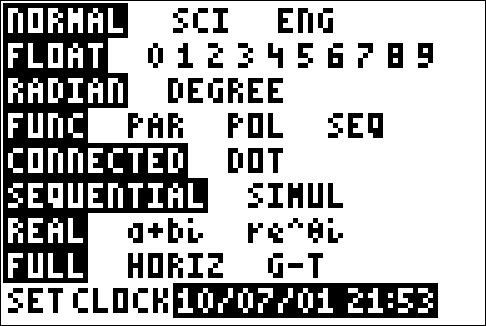
\includegraphics[width=2in]{./IntroTrigGraphics/CircularFunctions01.jpg} &
\hspace{0.75in} 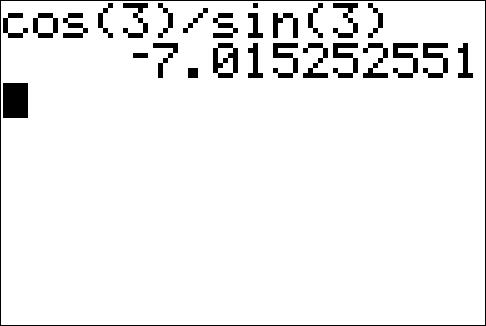
\includegraphics[width=2in]{./IntroTrigGraphics/CircularFunctions02.jpg}  \\ 

\end{tabular} 

\item  If $\theta$ is coterminal with $\frac{3 \pi}{2}$, then $\cos(\theta) = \cos\left(\frac{3 \pi}{2}\right) = 0$ and $\sin(\theta) = \sin\left(\frac{3 \pi}{2}\right) = -1$.  Attempting to compute $\tan(\theta) = \frac{\sin(\theta)}{\cos(\theta)}$ results in $\frac{-1}{0}$, so $\tan(\theta)$ is undefined.

\item  We are given that $\csc(\theta) = \frac{1}{\sin(\theta)} = -\sqrt{5}$ so $\sin(\theta) = -\frac{1}{\sqrt{5}} = -\frac{\sqrt{5}}{5}$.  As we saw in Section \ref{TheUnitCircle}, we can use the Pythagorean Identity, $\cos^{2}(\theta) + \sin^2(\theta) = 1$, to find $\cos(\theta)$ by knowing $\sin(\theta)$.  Substituting, we get $\cos^{2}(\theta) + \left(-\frac{\sqrt{5}}{5}\right)^2 = 1$, which gives $\cos^{2}(\theta) = \frac{4}{5}$, or $\cos(\theta) = \pm \frac{2 \sqrt{5}}{5}$.  Since $\theta$ is a Quadrant IV angle, $\cos(\theta) > 0$, so $\cos(\theta) = \frac{2 \sqrt{5}}{5}$.

\item \label{commontanmistake} If $\tan(\theta) = 3$, then $\frac{\sin(\theta)}{\cos(\theta)} = 3$.  Be careful - this does \textbf{NOT} mean we can take $\sin(\theta) = 3$ and $\cos(\theta) = 1$. Instead, from $\frac{\sin(\theta)}{\cos(\theta)} = 3$  we get: $\sin(\theta) = 3 \cos(\theta)$.  To relate $\cos(\theta)$ and $\sin(\theta)$, we once again employ the Pythagorean Identity, $\cos^{2}(\theta) + \sin^{2}(\theta) = 1$.  Solving $\sin(\theta) = 3 \cos(\theta)$ for $\cos(\theta)$, we find $\cos(\theta) = \frac{1}{3} \sin(\theta)$.  Substituting this into the Pythagorean Identity, we find  $\sin^{2}(\theta) + \left(\frac{1}{3} \sin(\theta)\right)^2 = 1$. Solving, we get $\sin^{2}(\theta) = \frac{9}{10}$ so $\sin(\theta) = \pm \frac{3 \sqrt{10}}{10}$.  Since $\pi < \theta < \frac{3\pi}{2}$, $\theta$ is  a Quadrant III angle.  This means $\sin(\theta) < 0$, so our final answer is  $\sin(\theta) = - \frac{3 \sqrt{10}}{10}$.  \qed

\end{enumerate}

\end{ex}

While the Reciprocal and Quotient Identities presented in Theorem \ref{recipquotid} allow us to always reduce problems involving secant, cosecant, tangent and cotangent to problems involving cosine and sine, it is not always convenient to do so.\footnote{As we shall see shortly, when solving equations involving secant and cosecant, we usually convert back to cosines and sines.  However, when solving for tangent or cotangent, we usually stick with what we're dealt.}  It is worth taking the time to memorize the tangent and cotangent values of the common angles summarized below.

\begin{center}

\textbf{Tangent and Cotangent Values of Common Angles}

\vspace{-.25in}

\setlength{\extrarowheight}{4pt}

\[ \begin{array}{|c|c||c|c|} \hline
 \theta (\mbox{degrees}) &  \theta (\mbox{radians}) & \tan(\theta) & \cot(\theta) \\ \hline
0^{\circ} & 0 & 0 & \text{undefined} \\ \hline
30^{\circ} & \frac{\pi}{6} & \frac{\sqrt{3}}{3} & \sqrt{3} \\ [2pt] \hline
45^{\circ} & \frac{\pi}{4} & 1 & 1 \\ [2pt] \hline
60^{\circ} & \frac{\pi}{3} & \sqrt{3} & \frac{\sqrt{3}}{3} \\ [2pt] \hline
90^{\circ} & \frac{\pi}{2} & \text{undefined} & 0 \\ [2pt] \hline
\end{array} \]

\setlength{\extrarowheight}{2pt}

\end{center}

Coupling Theorem \ref{recipquotid} with the Reference Angle Theorem, Theorem \ref{refanglethm}, we get the following.

\smallskip

\colorbox{ResultColor}{\bbm

\begin{thm} \label{genrefanglethm} \textbf{Generalized Reference Angle Theorem.}  The values of the circular functions of an angle, if they exist, are the same, up to a sign, of the corresponding circular functions of its reference angle.  More specifically, if $\alpha$ is the reference angle for $\theta$,  then: $\cos(\theta)  = \pm \cos(\alpha)$, $\sin(\theta)  = \pm \sin(\alpha)$, $\sec(\theta)  = \pm \sec(\alpha)$, $\csc(\theta)  = \pm \csc(\alpha)$, $\tan(\theta)  = \pm \tan(\alpha)$ and $\cot(\theta)  = \pm \cot(\alpha)$.  The choice of the ($\pm$) depends on the quadrant in which the terminal side of $\theta$ lies. \index{Reference Angle Theorem ! for the circular functions}

\end{thm}

\ebm}

\smallskip

We put Theorem \ref{genrefanglethm} to good use in the following example.

\begin{ex}  \label{solveforangle2}  Find all angles which satisfy the given equation.   

\begin{multicols}{3}

\begin{enumerate}

\item  $\sec(\theta) =2$

\item  $\tan(\theta) = \sqrt{3}$

\item  \label{cotangentisnegativeone} $\cot(\theta) = -1$.

\end{enumerate}

\end{multicols}

{\bf Solution.}

\begin{enumerate}

\item  To solve $\sec(\theta) = 2$, we convert to cosines and get $\frac{1}{\cos(\theta)} = 2$ or $\cos(\theta) = \frac{1}{2}$.  This is the exact same equation we solved in Example \ref{solveforangle}, number \ref{cosineishalf}, so we know the answer is:  $\theta = \frac{\pi}{3} + 2\pi k$ or $\theta = \frac{5\pi}{3} + 2\pi k$ for integers $k$.

\item From the table of common values, we see  $\tan\left(\frac{\pi}{3}\right) = \sqrt{3}$.  According to Theorem \ref{genrefanglethm}, we  know  the solutions to $\tan(\theta) = \sqrt{3}$ must, therefore, have a reference angle of $\frac{\pi}{3}$. Our next task is to determine in which quadrants the solutions to this equation lie. Since tangent is defined as the ratio $\frac{y}{x}$ of points $(x,y)$ on the Unit Circle with $x \neq 0$, tangent is positive when $x$ and $y$ have the same sign (i.e., when they are both positive or both negative.)  This happens in Quadrants I and III.  In Quadrant I, we get the solutions: $\theta = \frac{\pi}{3} + 2\pi k$ for integers $k$, and for Quadrant III, we get $\theta = \frac{4\pi}{3} + 2\pi k$ for integers $k$.  While these descriptions of the solutions are correct, they can be combined into one list as $\theta = \frac{\pi}{3} + \pi k$ for integers $k$. The latter form of the solution is best understood looking at the geometry of the situation in the diagram below.\footnote{See Example \ref{solveforangle} number \ref{cosineiszero} in Section \ref{TheUnitCircle} for another example of this kind of simplification of the solution.}
 

\begin{tabular}{cc}

\begin{mfpic}[15]{-5.25}{5.25}{-5.25}{5.5}
\axes
\tlabel(5.25,-0.5){\scriptsize $x$}
\tlabel(0.25,5.25){\scriptsize $y$}
\tlabel(4.6,-1){\scriptsize $1$}
\tlabel(0.25,4.6){\scriptsize $1$}
\xmarks{-4.5, 4.5}
\ymarks{-4.5 step 4.5 until 4.5}
\drawcolor[gray]{0.7}
\circle{(0,0),4.5}
\drawcolor[rgb]{0.33,0.33,0.33}
\arrow \polyline{(0,0), (2.5, 4.330)}
\arrow \reverse \arrow \parafcn{5, 55, 5}{1.5*dir(t)}
\tlabel(1.5, 1){$\frac{\pi}{3}$}
\point[3pt]{(0,0), (2.25, 3.8971)}
\end{mfpic} 

&

\hspace{.75in}

\begin{mfpic}[15]{-5.25}{5.25}{-5.25}{5.5}
\axes
\tlabel(5.25,-0.5){\scriptsize $x$}
\tlabel(0.25,5.25){\scriptsize $y$}
\tlabel(4.6,-1){\scriptsize $1$}
\tlabel(0.25,4.6){\scriptsize $1$}
\xmarks{-4.5, 4.5}
\ymarks{-4.5 step 4.5 until 4.5}
\drawcolor[gray]{0.7}
\circle{(0,0),4.5}
\drawcolor[rgb]{0.33,0.33,0.33}
\arrow \polyline{(0,0), (-2.5, -4.330)}
\arrow \reverse \arrow \parafcn{185, 235, 5}{2*dir(t)}
\tlabel(-2.6, -1.5){$\frac{\pi}{3}$}
\point[3pt]{(0,0), (-2.25, -3.8971)}
\arrow \dashed \polyline{(0,0), (2.5, 4.330)}
\arrow \reverse \arrow \parafcn{5, 55, 5}{1.5*dir(t)}
\tlabel(1.5, 1){$\frac{\pi}{3}$}
\tlabel(-1.5, 2){$\pi$}
\point[3pt]{(2.25, 3.8971)}
\arrow \reverse \arrow \parafcn{65, 235, 5}{1.5*dir(t)}
\end{mfpic} 
\end{tabular}
  

\item  From the table of common values, we see that $\frac{\pi}{4}$ has a cotangent of $1$, which means the solutions to $\cot(\theta) = -1$ have a reference angle of $\frac{\pi}{4}$. To find the quadrants in which our solutions lie, we note that $\cot(\theta) = \frac{x}{y}$ for a point $(x,y)$ on the Unit Circle where $y \neq 0$. If $\cot(\theta)$ is negative, then $x$ and $y$ must have different signs (i.e., one positive and one negative.)  Hence, our solutions lie in Quadrants II and IV.  Our Quadrant II solution is $\theta = \frac{3\pi}{4} + 2\pi k$, and for Quadrant IV, we get $\theta = \frac{7\pi}{4} + 2\pi k$ for integers $k$.  Can these lists be combined?  Indeed they can - one such way to capture all the solutions is:  $\theta = \frac{3\pi}{4} + \pi k$ for integers $k$.


\begin{tabular}{cc}

\begin{mfpic}[15]{-5.25}{5.25}{-5.25}{5.5}
\axes
\tlabel(5.25,-0.5){\scriptsize $x$}
\tlabel(0.25,5.25){\scriptsize $y$}
\tlabel(4.6,-1){\scriptsize $1$}
\tlabel(0.25,4.6){\scriptsize $1$}
\xmarks{-4.5, 4.5}
\ymarks{-4.5 step 4.5 until 4.5}
\drawcolor[gray]{0.7}
\circle{(0,0),4.5}
\drawcolor[rgb]{0.33,0.33,0.33}
\arrow \polyline{(0,0), (-3.5355, 3.5355)}
\arrow \reverse \arrow \parafcn{140, 175, 5}{1.5*dir(t)}
\tlabel[cc](-2, 1){$\frac{\pi}{4}$}
\point[3pt]{(0,0), (-3.1820, 3.1820)}
\end{mfpic} 

&

\hspace{.75in}

\begin{mfpic}[15]{-5.25}{5.25}{-5.25}{5.5}
\axes
\tlabel(5.25,-0.5){\scriptsize $x$}
\tlabel(0.25,5.25){\scriptsize $y$}
\tlabel(4.6,-1){\scriptsize $1$}
\tlabel(0.25,4.6){\scriptsize $1$}
\xmarks{-4.5, 4.5}
\ymarks{-4.5 step 4.5 until 4.5}
\drawcolor[gray]{0.7}
\circle{(0,0),4.5}
\drawcolor[rgb]{0.33,0.33,0.33}
\arrow \polyline{(0,0), (3.5355, -3.5355)}
\arrow \reverse \arrow \parafcn{320, 355, 5}{1.5*dir(t)}
\tlabel[cc](2, -1){$\frac{\pi}{4}$}
\tlabel[cc](-1.77, -1.77){$\pi$}
\point[3pt]{(0,0), (3.1820, -3.1820), (-3.1820, 3.1820)}
\arrow \dashed \polyline{(0,0), (-3.5355, 3.5355)}
\arrow \reverse \arrow \parafcn{140, 175, 5}{2*dir(t)}
\arrow \reverse \arrow \parafcn{140, 310, 5}{1.5*dir(t)}
\tlabel[cc](-2.31, 0.96){$\frac{\pi}{4}$}
\end{mfpic}
\end{tabular}

\end{enumerate}

\vspace{-.3in} \qed

\end{ex}

We have already seen the importance of identities in trigonometry.  Our next task is to use use the Reciprocal and Quotient Identities found in Theorem \ref{recipquotid} coupled with the Pythagorean Identity found in Theorem \ref{cosinesinepythid} to derive new Pythagorean-like identities for the remaining four circular functions.   Assuming $\cos(\theta) \neq 0$, we may start with $\cos^{2}(\theta) + \sin^{2}(\theta) = 1$ and divide both sides by $\cos^{2}(\theta)$ to obtain $1 + \frac{\sin^{2}(\theta)}{\cos^{2}(\theta)} = \frac{1}{\cos^{2}(\theta)}$.  Using properties of exponents along with the Reciprocal and Quotient Identities, this reduces to $1 + \tan^{2}(\theta) = \sec^{2}(\theta)$.  If $\sin(\theta) \neq 0$, we can divide both sides of the identity $\cos^{2}(\theta) + \sin^{2}(\theta) = 1$ by $\sin^{2}(\theta)$, apply Theorem \ref{recipquotid} once again,  and obtain $\cot^{2}(\theta) + 1 = \csc^{2}(\theta)$.  These three Pythagorean Identities are worth memorizing and they, along with some of their other common forms, are summarized in the following theorem.

\smallskip

\colorbox{ResultColor}{\bbm

\begin{thm} \label{pythids}  \textbf{The Pythagorean Identities:} \index{Pythagorean Identities}

\begin{enumerate}

\item $\cos^{2}(\theta) + \sin^{2}(\theta) = 1$.

\textbf{Common Alternate Forms:}

\begin{itemize}

\item  $1 - \sin^{2}(\theta) = \cos^{2}(\theta)$

\item  $1 - \cos^{2}(\theta) = \sin^{2}(\theta)$

\end{itemize}

\item $1 + \tan^{2}(\theta) = \sec^{2}(\theta)$, provided $\cos(\theta) \neq 0$.

\textbf{Common Alternate Forms:}

\begin{itemize}

\item  $\sec^{2}(\theta) - \tan^{2}(\theta) = 1$

\item  $\sec^{2}(\theta) - 1 = \tan^{2}(\theta)$

\end{itemize}

\item $1 + \cot^{2}(\theta) = \csc^{2}(\theta)$, provided $\sin(\theta) \neq 0$.

\textbf{Common Alternate Forms:}

\begin{itemize}

\item  $\csc^{2}(\theta) - \cot^{2}(\theta) = 1$

\item  $\csc^{2}(\theta) - 1 = \cot^{2}(\theta)$

\end{itemize}

\end{enumerate}

\end{thm}

\ebm}

\smallskip

Trigonometric identities play an important role in not just Trigonometry, but in Calculus as well.  We'll use them in this book to find the values of the circular functions of an angle and solve equations and inequalities.  In Calculus, they are needed to simplify otherwise complicated expressions.  In the next example, we make good use of the Theorems \ref{recipquotid} and \ref{pythids}.

\begin{ex} \label{idornotex1} Verify the following identities. Assume that all quantities are defined.

\begin{multicols}{2}

\begin{enumerate}

\item  $\dfrac{1}{\csc(\theta)} = \sin(\theta)$

\item  $\tan(\theta) = \sin(\theta) \sec(\theta)$ \vphantom{$\dfrac{1}{\csc(\theta)}$}

\setcounter{HW}{\value{enumi}}

\end{enumerate}

\end{multicols}

\begin{multicols}{2}

\begin{enumerate}

\setcounter{enumi}{\value{HW}}

\item  $(\sec(\theta) - \tan(\theta)) (\sec(\theta) + \tan(\theta)) = 1$ \vphantom{$\dfrac{\sec(\theta)}{1 - \tan(\theta)}$}

\item  $\dfrac{\sec(\theta)}{1 - \tan(\theta)} = \dfrac{1}{\cos(\theta) - \sin(\theta)}$

\setcounter{HW}{\value{enumi}}

\end{enumerate}

\end{multicols}

\begin{multicols}{2}

\begin{enumerate}

\setcounter{enumi}{\value{HW}}

\item  $6\sec(\theta) \tan(\theta) = \dfrac{3}{1-\sin(\theta)} - \dfrac{3}{1 + \sin(\theta)}$

\item  \label{pythconjex} $\dfrac{\sin(\theta)}{1 - \cos(\theta)} = \dfrac{1 + \cos(\theta)}{\sin(\theta)}$

\end{enumerate}

\end{multicols}

{\bf Solution.}  In verifying identities, we typically start with the more complicated side of the equation and use known identities to \textit{transform} it into the other side of the equation. 

\begin{enumerate} 

\item  To verify $\frac{1}{\csc(\theta)} = \sin(\theta)$, we start with the left side.  Using $\csc(\theta) = \frac{1}{\sin(\theta)}$, we get:  \[ \dfrac{1}{\csc(\theta)} = \dfrac{1}{\frac{1}{\sin(\theta)}} = \sin(\theta),\]

\enlargethispage{.1in} which is what we were trying to prove.

\item Starting with the right hand side of $\tan(\theta) = \sin(\theta) \sec(\theta)$, we use $\sec(\theta) = \frac{1}{\cos(\theta)}$ and find:  \[ \sin(\theta) \sec(\theta) = \sin(\theta) \dfrac{1}{\cos(\theta)} = \dfrac{\sin(\theta)}{\cos(\theta)} = \tan(\theta),\]

where the last equality is courtesy of Theorem \ref{recipquotid}.

\item Expanding the left hand side of the equation gives:  $(\sec(\theta) - \tan(\theta)) (\sec(\theta) + \tan(\theta)) = \sec^{2}(\theta) - \tan^{2}(\theta)$.  According to Theorem \ref{pythids}, $\sec^{2}(\theta) - \tan^{2}(\theta) = 1$.  Putting it all together, \[(\sec(\theta) - \tan(\theta)) (\sec(\theta) + \tan(\theta)) = \sec^{2}(\theta) - \tan^{2}(\theta)  = 1.\]


\item  While both sides of our last identity contain fractions, the left side affords us more opportunities to use our identities.\footnote{Or, to put to another way, earn more partial credit if this were an exam question!} Substituting $\sec(\theta) = \frac{1}{\cos(\theta)}$ and $\tan(\theta) = \frac{\sin(\theta)}{\cos(\theta)}$, we get:


\[ \begin{array}{rcl} \dfrac{\sec(\theta)}{1 - \tan(\theta)} & = & \dfrac{ \dfrac{1}{\cos(\theta)}}{1 - \dfrac{\sin(\theta)}{\cos(\theta)}} = \dfrac{ \dfrac{1}{\cos(\theta)}}{1 - \dfrac{\sin(\theta)}{\cos(\theta)}} \cdot \dfrac{\cos(\theta)}{\cos(\theta)} \\ [.4in]
 & = & \dfrac{\left( \dfrac{1}{\cos(\theta)} \right) ( \cos(\theta) )}{\left(1 - \dfrac{\sin(\theta)}{\cos(\theta)}\right)(\cos(\theta))} = \dfrac{1}{(1)(\cos(\theta)) - \left(\dfrac{\sin(\theta)}{\cos(\theta)}\right)(\cos(\theta))} \\ [.4in]
                                                           & = & \dfrac{1}{\cos(\theta) - \sin(\theta)}, \end{array} \]
which is exactly what we had set out to show.  

\item  The right hand side of the equation seems to hold more promise.  We get common denominators and add:

\[ \begin{array}{rcl}

\dfrac{3}{1-\sin(\theta)} - \dfrac{3}{1 + \sin(\theta)} & = & \dfrac{3(1 + \sin(\theta))}{(1-\sin(\theta))(1 + \sin(\theta))} - \dfrac{3(1-\sin(\theta))}{(1 + \sin(\theta))(1-\sin(\theta))} \\ [.25in]
                                                        & = & \dfrac{3 + 3\sin(\theta)}{1 - \sin^{2}(\theta)} - \dfrac{3 - 3\sin(\theta)}{1 - \sin^{2}(\theta)} \\ [.25in]
                                                        & = & \dfrac{(3 + 3\sin(\theta)) - (3 - 3\sin(\theta))}{1 - \sin^{2}(\theta)} \\ [.25in]                                                        																																	& = & \dfrac{6 \sin(\theta)}{1 - \sin^{2}(\theta)} \end{array} \]

At this point, it is worth pausing to remind ourselves of our goal.  We wish to transform this expression into $6\sec(\theta) \tan(\theta)$.  Using a reciprocal and quotient identity, we find $6\sec(\theta) \tan(\theta) = 6 \left(\frac{1}{\cos(\theta)}\right) \left(\frac{\sin(\theta)}{\cos(\theta)}\right)$.  In other words, we need to get cosines in our denominator. Theorem \ref{pythids} tells us $1 -  \sin^{2}(\theta) = \cos^{2}(\theta)$ so we get:

\[ \begin{array}{rcl}

\dfrac{3}{1-\sin(\theta)} - \dfrac{3}{1 + \sin(\theta)} & = & \dfrac{6 \sin(\theta)}{1 - \sin^{2}(\theta)}= \dfrac{6 \sin(\theta)}{\cos^{2}(\theta)} \\ [.25in]
& = &  6 \left(\dfrac{1}{\cos(\theta)}\right)\left( \dfrac{\sin(\theta)}{\cos(\theta)}\right) = 6 \sec(\theta) \tan(\theta) \\ \end{array} \]

\item  It is debatable which side of the identity is more complicated.  One thing which stands out is that the denominator on the left hand side is $1-\cos(\theta)$, while the numerator of the right hand side is $1+\cos(\theta)$.  This suggests the strategy of starting with the left hand side and multiplying the numerator and denominator by the quantity $1+\cos(\theta)$:

\[ \begin{array}{rcl}


\dfrac{\sin(\theta)}{1 - \cos(\theta)} & = & \dfrac{\sin(\theta)}{(1 - \cos(\theta))} \cdot \dfrac{(1 + \cos(\theta))}{(1 + \cos(\theta))} = \dfrac{\sin(\theta)(1 + \cos(\theta))}{(1 - \cos(\theta))(1 + \cos(\theta))} \\ [.25in]
& = & \dfrac{\sin(\theta)(1 + \cos(\theta))}{1 - \cos^{2}(\theta)} = \dfrac{\sin(\theta)(1 + \cos(\theta))}{\sin^{2}(\theta)} \\ [.25in]
& = & \dfrac{\cancel{\sin(\theta)}(1 + \cos(\theta))}{\cancel{\sin(\theta)}\sin(\theta)} = \dfrac{1 + \cos(\theta)}{\sin(\theta)} \end{array} \]

\vspace{-.1in} \qed

\end{enumerate}

\end{ex}

In Example \ref{idornotex1} number \ref{pythconjex} above,  we see that multiplying  $1-\cos(\theta)$ by $1+\cos(\theta)$ produces a difference of squares that can be simplified to one term using Theorem \ref{pythids}.  This is exactly the same kind of phenomenon that occurs when we multiply expressions such as $1 - \sqrt{2}$ by $1+\sqrt{2}$ or $3 - 4i$ by $3+4i$. (Can you recall instances from Algebra where we did such things?) For this reason, the quantities $(1-\cos(\theta))$ and $(1+\cos(\theta))$ are called `Pythagorean Conjugates.'  Below is a list of other common Pythagorean Conjugates.  

\smallskip

\phantomsection
\label{PythagoreanConjugates}
\smallskip
\colorbox{ResultColor}{\bbm

\smallskip

\centerline{\textbf{Pythagorean Conjugates}}  \index{Pythagorean Conjugates}

\begin{itemize}

\item $1 - \cos(\theta)$ and  $1+\cos(\theta)$:  $(1-\cos(\theta))(1+\cos(\theta)) = 1 - \cos^{2}(\theta) = \sin^{2}(\theta)$

\item  $1-\sin(\theta)$ and $1 + \sin(\theta)$:  $(1-\sin(\theta))(1+\sin(\theta)) = 1 - \sin^{2}(\theta) = \cos^{2}(\theta)$

\item  $\sec(\theta)-1$ and $\sec(\theta)+1$:  $(\sec(\theta)-1)(\sec(\theta)+1) = \sec^{2}(\theta) - 1 =  \tan^{2}(\theta)$

\item  $\sec(\theta)-\tan(\theta)$ and $\sec(\theta)+\tan(\theta)$:  $(\sec(\theta)-\tan(\theta))(\sec(\theta)+\tan(\theta)) = \sec^{2}(\theta) - \tan^{2}(\theta) = 1$

\item  $\csc(\theta)-1$ and $\csc(\theta)+1$:  $(\csc(\theta)-1)(\csc(\theta)+1) = \csc^{2}(\theta) - 1 =  \cot^{2}(\theta)$

\item  $\csc(\theta)-\cot(\theta)$ and $\csc(\theta)+\cot(\theta)$:  $(\csc(\theta)-\cot(\theta))(\csc(\theta)+\cot(\theta)) = \csc^{2}(\theta) - \cot^{2}(\theta) = 1$

\smallskip

\end{itemize}

\ebm}

Verifying trigonometric identities requires a healthy mix of tenacity and inspiration.  You will need to spend many hours struggling with them just to become proficient in the basics.  Like many things in life, there is no short-cut here -- there is no complete algorithm for verifying identities.  Nevertheless, a summary of some strategies which  may be helpful (depending on the situation) is provided below and ample practice is provided for you in the Exercises.

\phantomsection
\label{IdentityHelp}

\colorbox{ResultColor}{\bbm

\medskip

\centerline{\textbf{Strategies for Verifying Identities}} 

\begin{itemize}

\item  Try working on the more complicated side of the identity.

\item Use the Reciprocal and Quotient Identities in Theorem \ref{recipquotid} to write functions on one side of the identity in terms of the functions on the other side of the identity.  Simplify the resulting complex fractions.

\item Add rational expressions with unlike denominators by obtaining common denominators.

\item  Use the Pythagorean Identities in Theorem \ref{pythids} to `exchange' sines and cosines, secants and tangents, cosecants and cotangents, and simplify sums or differences of squares to one term. 

\item Multiply numerator \textbf{and} denominator by Pythagorean
Conjugates in order to take advantage of the Pythagorean Identities in  Theorem \ref{pythids}.

\item If you find yourself stuck working with one side of the identity, try starting with the other side of the identity and see if you can find a way to bridge the two parts of your work.


\end{itemize}

\ebm}

\subsection{Beyond the Unit Circle}
\label{circularfunctionsbeyond}

In Section \ref{TheUnitCircle}, we generalized the cosine and sine functions from coordinates on the Unit Circle to coordinates on circles of radius $r$.  Using Theorem \ref{cosinesinecircle} in conjunction with Theorem \ref{pythids}, we generalize the remaining circular functions in kind.

\smallskip

\colorbox{ResultColor}{\bbm

\begin{thm} \label{circularfunctionscircle} Suppose $Q(x,y)$ is the point on the terminal side of an angle $\theta$ (plotted in standard position) which lies on the circle of radius $r$,  $x^2+y^2 = r^2$. Then:

\begin{itemize}

\item $\sec(\theta) = \dfrac{r}{x} = \dfrac{\sqrt{x^2+y^2}}{x}$, provided $x \neq 0$. \index{secant ! of an angle}

\item $\csc(\theta) = \dfrac{r}{y} = \dfrac{\sqrt{x^2+y^2}}{y}$, provided $y \neq 0$. \index{cosecant ! of an angle}

\item $\tan(\theta) = \dfrac{y}{x}$, provided $x \neq 0$. \index{tangent ! of an angle}

\item $\cot(\theta) = \dfrac{x}{y}$, provided $y \neq 0$. \index{cotangent ! of an angle}

\end{itemize}

\end{thm}

\ebm}

\pagebreak

\begin{ex} \label{circularfunctionscircleex} $~$

\begin{enumerate}

\item  Suppose the terminal side of $\theta$, when plotted in standard position, contains the point $Q(3,-4)$.  Find the values of the six circular functions of $\theta$.

\item  Suppose $\theta$ is a Quadrant IV angle with $\cot(\theta) = -4$.  Find the values of the five remaining circular functions of $\theta$.

\end{enumerate}

{\bf Solution.}

\begin{enumerate}

\item    Since $x = 3$ and $y=-4$, $r = \sqrt{x^2 + y^2} = \sqrt{(3)^2+(-4)^2} = \sqrt{25} = 5$. Theorem \ref{circularfunctionscircle} tells us $\cos(\theta) = \frac{3}{5}$, $\sin(\theta) = -\frac{4}{5}$, $\sec(\theta) = \frac{5}{3}$, $\csc(\theta) = -\frac{5}{4}$, $\tan(\theta) = -\frac{4}{3}$ and $\cot(\theta) = - \frac{3}{4}$.

\item In order to use Theorem \ref{circularfunctionscircle}, we need to find a point $Q(x,y)$ which lies on the terminal side of $\theta$, when $\theta$ is plotted in standard position.  We have that $\cot(\theta) = -4 =  \frac{x}{y}$,  and since $\theta$ is a Quadrant IV angle, we also know $x>0$ and $y< 0$.  Viewing $-4 = \frac{4}{-1}$, we may choose\footnote{We may choose \textit{any} values $x$ and $y$ so long as $x>0$, $y<0$ and $\frac{x}{y} = -4$.  For example, we could choose $x=8$ and $y=-2$.  The fact that all such points lie on the terminal side of $\theta$ is a consequence of the fact that the terminal side of $\theta$ is the portion of the line with slope $-\frac{1}{4}$ which extends from the origin into Quadrant IV.}   $x = 4$ and $y = -1$ so that $r = \sqrt{x^2+y^2} = \sqrt{(4)^2 + (-1)^2} = \sqrt{17}$.  Applying Theorem \ref{circularfunctionscircle} once more, we find $\cos(\theta) = \frac{4}{\sqrt{17}} = \frac{4 \sqrt{17}}{17}$,  $\sin(\theta) =- \frac{1}{\sqrt{17}} = -\frac{\sqrt{17}}{17}$, $\sec(\theta) = \frac{\sqrt{17}}{4}$, $\csc(\theta) = - \sqrt{17}$ and $\tan(\theta) = -\frac{1}{4}$. \qed  

\end{enumerate}

\end{ex}

We may also specialize Theorem \ref{circularfunctionscircle} to the case of acute angles $\theta$ which reside in a right triangle, as visualized below.  

\begin{center}

\begin{mfpic}[18]{-5}{5}{-5}{5}
\polyline{(-4.330,0), (4.330,0), (4.330,5), (-4.330,0)}
\arrow \reverse \arrow \shiftpath{(-4.330,0)} \parafcn{5, 25, 5}{3*dir(t)}
\tlabel(-1, 0.6){$\theta$}
\tlabel(0,-0.75){$a$}
\tlabel(4.75,2.25){$b$}
\tlabel(0,3){$c$}
\polyline{(3.93, 0), (3.93, 0.4), (4.33, 0.4)}
\end{mfpic}

\end{center}

\colorbox{ResultColor}{\bbm

\begin{thm} \label{circularfunctionstriangle}  Suppose $\theta$ is an acute angle residing in a right triangle.  If the length of the side adjacent to $\theta$ is $a$, the length of the side opposite $\theta$ is $b$, and the length of the hypotenuse is $c$, then \[\begin{array}{llll} \tan(\theta) = \dfrac{b}{a} \;\;\;\;\;\; & \sec(\theta) = \dfrac{c}{a} \;\;\;\;\;\; & \csc(\theta) = \dfrac{c}{b} \;\;\;\;\;\; & \cot(\theta) = \dfrac{a}{b}  \end{array}\]

\end{thm}

\ebm}

\bigskip

The following example uses Theorem \ref{circularfunctionstriangle} as well as the concept of an `angle of inclination.'  The \index{angle ! of inclination} angle of inclination (or \index{angle ! of elevation} angle of elevation) of an object refers to the angle whose initial side is some kind of base-line (say, the ground), and whose terminal side is the line-of-sight to an object above the base-line.  This is represented schematically below.

\phantomsection
\label{angleofelevation}

\begin{center}

\begin{mfpic}[18]{-5}{5}{-5}{5}
\polyline{(-4.330,0), (5,0)}
\dashed \polyline{(-4.330,0), (4.330,5)}
\arrow \shiftpath{(-4.330,0)} \parafcn{5, 25, 5}{3*dir(t)}
\tlabel(-1, 0.6){$\theta$}
\tlabel[cc](0,-1){`base line'}
\plotsymbol[3pt]{Asterisk}{(4.330,5)}
\tlabel(4.5,4.5){object}
\end{mfpic} 

\smallskip

The angle of inclination from the base line to the object is $\theta$
\end{center}

\begin{ex} \label{circularfunctionstriangleex} $~$

\begin{enumerate}

\item  The angle of inclination from a point on the ground 30 feet away to the top of Lakeland's Armington Clocktower\footnote{Named in honor of Raymond Q. Armington, Lakeland's Clocktower has been a part of campus since 1972.} is  $60^{\circ}$.  Find the height of the Clocktower to the nearest foot.

\item  In order to determine the height of a California Redwood tree, two sightings from the ground, one 200 feet directly behind the other, are made.  If the angles of inclination were $45^{\circ}$ and $30^{\circ}$, respectively, how tall is the tree to the nearest foot?

\end{enumerate}

{\bf Solution.}

\begin{enumerate}

\item  We can represent the problem situation using a right triangle as shown below.  If we let $h$ denote the height of the tower, then Theorem \ref{circularfunctionstriangle} gives $\tan\left(60^{\circ}\right) = \frac{h}{30}$.  From this we get $h = 30 \tan\left(60^{\circ}\right) = 30 \sqrt{3} \approx 51.96$.  Hence, the Clocktower is approximately $52$ feet tall.

\begin{center}

\begin{mfpic}[15]{-5}{5}{-5}{5}
\polyline{(0,-4.330), (5,-4.330), (5,4.330), (0,-4.330)}
\arrow \shiftpath{(0,-4.330)} \parafcn{5, 55, 5}{1.5*dir(t)}
\tlabel(1.6,-3.75){$60^{\circ}$}
\tlabel(2,-5.5){$30$ ft.}
\tlabel(5.25,0){$h$ ft.}
\polyline{(4.6, -4.330), (4.6,-3.930), (5, -3.930)}
\end{mfpic}

Finding the height of the Clocktower

\end{center}

\item  Sketching the problem situation below, we find ourselves with two unknowns: the height $h$ of the tree and the distance $x$ from the base of the tree to the first observation point. 

\begin{center}

\begin{mfpic}[18]{-7}{5}{-5}{5}
\polyline{(-2.5,0), (2.5,0), (2.5,5), (-2.5,0)}
\polyline{(-6,0), (2.5,0), (2.5,5), (-6,0)}
\arrow \shiftpath{(-2.5,0)} \parafcn{5, 35, 5}{1.5*dir(t)}
\tlabel(-0.8, 0.4){$45^{\circ}$}
\tlabel(-4, 0.4){$30^{\circ}$}
\arrow \shiftpath{(-6,0)} \parafcn{5, 25, 5}{1.75*dir(t)}
\tlabel(-5,-1){$200$ ft.}
\tlabel(-1,-1){$x$ ft.}
\tlabel(2.75,2.25){$h$ ft.}
\polyline{(2.25, 0), (2.25, 0.25), (2.5, 0.25)}
\point[3pt]{(-2.5,0), (-6,0)}
\end{mfpic} 

Finding the height of a California Redwood
\end{center}


Using Theorem \ref{circularfunctionstriangle}, we get a pair of equations:  $\tan\left(45^{\circ}\right) = \frac{h}{x}$ and $\tan\left(30^{\circ}\right) = \frac{h}{x+200}$.  Since $\tan\left(45^{\circ}\right) = 1$, the first equation gives $\frac{h}{x} = 1$, or $x = h$.  Substituting this into the second equation gives $\frac{h}{h+200} = \tan\left(30^{\circ}\right) = \frac{\sqrt{3}}{3}$.  Clearing fractions,  we get $3h = (h+200) \sqrt{3}$.  The result is a linear equation for $h$, so we proceed to expand the right hand side and gather all the terms involving $h$ to one side.

\[ \begin{array}{rcl}

3h & = & (h+200)\sqrt{3} \\ [5pt]
3h & = & h \sqrt{3} + 200 \sqrt{3} \\ [5pt]
3h - h \sqrt{3} & = & 200 \sqrt{3} \\ [5pt]
(3-\sqrt{3}) h & = & 200 \sqrt{3} \\ [5pt]
h & = & \dfrac{200\sqrt{3}}{3-\sqrt{3}} \approx 273.20 \\ \end{array} \] 


Hence, the tree is approximately $273$ feet tall.  \qed

\end{enumerate}

\end{ex} 

As we did in Section \ref{cosinesinebeyond}, we may consider all six circular functions as functions of real numbers. At this stage, there are three equivalent ways to define the functions $\sec(t)$, $\csc(t)$, $\tan(t)$ and $\cot(t)$ for real numbers $t$.  First, we could go through the formality of the wrapping function on page \pageref{wrappingfunction} and define these functions as the appropriate ratios of  $x$ and $y$ coordinates of points on the Unit Circle;  second, we could define them by associating the real number $t$ with the angle $\theta = t$ radians so that the value of the trigonometric function of $t$ coincides with that of  $\theta$;  lastly, we could simply define them using the Reciprocal and Quotient Identities as combinations of the functions $f(t) = \cos(t)$ and $g(t) = \sin(t)$.  Presently, we adopt the last approach.  We now set about determining the domains and ranges of the remaining four circular functions.  Consider the function $F(t) = \sec(t)$ defined as $F(t) = \sec(t) = \frac{1}{\cos(t)}$.  We know $F$ is undefined whenever $\cos(t) = 0$.  From Example \ref{solveforangle} number \ref{cosineiszero}, we know $\cos(t) = 0$ whenever $t = \frac{\pi}{2} + \pi k$ for integers $k$.  Hence, our domain for $F(t) = \sec(t)$, in set builder notation is  $\{ t : t \neq  \frac{\pi}{2} + \pi k, \text{for integers $k$} \}$.  To get a better understanding what set of real numbers we're dealing with, it pays to write out and graph this set.  Running through a few values of $k$, we find the domain to be  $\{ t : t \neq  \pm \frac{\pi}{2}, \, \pm \frac{3\pi}{2}, \, \pm \frac{5\pi}{2}, \, \ldots \}$.  Graphing this set on the number line we get


\begin{center}

\begin{mfpic}[15]{-6}{6}{-1}{2}
\arrow \reverse \arrow \polyline{(-6,0), (6,0)}
\xmarks{-5,-3,-1,1,3,5}
\tlpointsep{4pt}
\axislabels {x}{{\small $-\frac{5\pi}{2} \hspace{7pt}$} -5,{\small $-\frac{3\pi}{2} \hspace{7pt}$} -3, {\small $-\frac{\pi}{2} \hspace{7pt}$} -1,{\small $0$} 0,{\small $\frac{\pi}{2}$} 1,  {\small $\frac{3\pi}{2}$} 3,  {\small $\frac{5\pi}{2}$} 5}

\penwd{1.5}
\arrow \reverse \arrow \polyline{(-5.75,1), (5.75,1)}

\penwd{0.75}

\gclear \circle{(-5,1),0.15}
\circle{(-5,1),0.15}

\gclear \circle{(-3,1),0.15}
\circle{(-3,1),0.15}

\gclear \circle{(-1,1),0.15}
\circle{(-1,1),0.15}

\gclear \circle{(5,1),0.15}
\circle{(5,1),0.15}

\gclear \circle{(3,1),0.15}
\circle{(3,1),0.15}

\gclear \circle{(1,1),0.15}
\circle{(1,1),0.15}

\end{mfpic}

\end{center}

Using interval notation to describe this set, we get  \[ \ldots \cup \left( -\frac{5\pi}{2}, -\frac{3\pi}{2}\right) \cup \left( -\frac{3\pi}{2}, -\frac{\pi}{2}\right) \cup  \left(-\frac{\pi}{2}, \frac{\pi}{2}\right) \cup \left(\frac{\pi}{2}, \frac{3\pi}{2}\right) \cup  \left(\frac{3\pi}{2}, \frac{5\pi}{2}\right) \cup \ldots \]

This is cumbersome, to say the least!  In order to write this in a more compact way, we note that from the set-builder description of the domain, the $k$th point excluded from the domain, which we'll call $x_{\mbox{\tiny $k$}}$, can be found by the formula $x_{\mbox{\tiny $k$}} =  \frac{\pi}{2} + \pi k$.  (We are using sequence notation from Chapter \ref{SequencesandSeries}.)  Getting a common denominator and factoring out the $\pi$ in the numerator, we get  $x_{\mbox{\tiny $k$}} = \frac{(2k+1)\pi}{2}$.  The domain consists of the intervals determined by successive points $x_{\mbox{\tiny $k$}}$:   $\left(x_{\mbox{\tiny $k$}}, x_{\mbox{\tiny $k+1$}}\right) = \left( \frac{(2k+1)\pi}{2},  \frac{(2k+3)\pi}{2}\right)$.  In order to capture all of the intervals in the domain, $k$ must run through all of the integers, that is, $k = 0$, $\pm 1$, $\pm 2$, \ldots.  The way we denote taking the union of infinitely many intervals like this is to use what we call in this text \index{extended interval notation}\index{interval ! notation, extended}\textbf{extended interval notation}.  The domain of $F(t) = \sec(t)$ can now be written as

\[ \bigcup_{k = -\infty}^{\infty} \left( \frac{(2k+1)\pi}{2}, \frac{(2k+3) \pi}{2} \right) \]

\phantomsection
\label{extendedinterval}

The reader should compare this notation with summation notation introduced in Section \ref{Summation}, in particular the notation used to describe geometric series in Theorem \ref{geoseries}.  In the same way the index $k$ in the series \[\displaystyle{\sum_{k = 1}^{\infty} a r^{k-1}}\] can never equal the upper limit $\infty$, but rather, ranges through all of the natural numbers, the index $k$ in the union \[\displaystyle{\bigcup_{k = -\infty}^{\infty} \left( \frac{(2k+1)\pi}{2}, \frac{(2k+3) \pi}{2} \right)}\] can never actually be $\infty$ or $-\infty$, but rather, this conveys the idea that $k$ ranges through all of the integers.  Now that we have painstakingly determined the domain of $F(t) = \sec(t)$, it is time to discuss the range.  Once again, we appeal to the definition $F(t) = \sec(t) = \frac{1}{\cos(t)}$.  The range of $f(t) = \cos(t)$ is $[-1,1]$, and since $F(t) = \sec(t)$ is  undefined when $\cos(t) = 0$, we split our discussion into two cases: when $0 < \cos(t) \leq 1$ and when $-1 \leq \cos(t) < 0$.  If $0 < \cos(t) \leq 1$, then we can divide the inequality $\cos(t) \leq 1$ by  $\cos(t)$ to obtain  $\sec(t) = \frac{1}{\cos(t)} \geq 1$.  Moreover, using the notation introduced in Section \ref{RationalGraphs}, we have that as  $\cos(t) \rightarrow 0^{+}$, $\sec(t)  = \frac{1}{\cos(t)} \approx \frac{1}{\mbox{\tiny very small $(+)$}} \approx \mbox{very big $(+)$}$.  In other words, as $\cos(t) \rightarrow 0^{+}, \sec(t) \rightarrow \infty$. If, on the other hand, if $-1 \leq \cos(t) < 0$, then dividing by $\cos(t)$ causes a reversal of the inequality so that $\sec(t) = \frac{1}{\sec(t)} \leq -1$.  In this case, as $\cos(t) \rightarrow 0^{-}$, $\sec(t)  = \frac{1}{\cos(t)} \approx \frac{1}{\mbox{\tiny very small $(-)$}} \approx \mbox{very big $(-)$}$, so that as $\cos(t) \rightarrow 0^{-}$, we get $\sec(t) \rightarrow -\infty$. Since $f(t) = \cos(t)$ admits all of the values in $[-1,1]$, the function $F(t) = \sec(t)$ admits all of the values in $(-\infty, -1] \cup [1,\infty)$.  Using set-builder notation, the range of $F(t) = \sec(t)$ can be written as $\{ u : \text{$u \leq -1$ or $u \geq 1$} \}$, or, more succinctly,\footnote{Using Theorem \ref{absolutevalueineq} from Section \ref{Inequalities}.} as  $\{ u :|u| \geq 1 \}$.\footnote{Notice we have used the variable `$u$' as the `dummy variable' to describe the range elements.  While there is no mathematical reason to do this (we are describing a set of real numbers, and, as such, could use $t$ again) we choose $u$ to help solidify the idea that these real numbers are the outputs from the inputs, which we have been calling $t$.}  Similar arguments can be used to determine the domains and ranges of the remaining three circular functions: $\csc(t)$, $\tan(t)$ and $\cot(t)$.  The reader is encouraged to do so.  (See the Exercises.)  For now, we gather these facts into the theorem below.

\smallskip

\colorbox{ResultColor}{\bbm

\begin{thm} \label{circularfunctionsdomainrange}  \textbf{Domains and Ranges of the Circular Functions} 

\vspace{.2in}

\begin{tabular}{ll}

\hspace{.3in} $\bullet \, $ The function $f(t) = \cos(t)$ & \hspace{.8in} $\bullet \, $ The function $g(t) = \sin(t)$ \\
  & \\
\hspace{.5in} -- has domain $(-\infty, \infty)$ & \hspace{1in} -- has domain $(-\infty, \infty)$ \\ [4pt]
\hspace{.5in} -- has range $[-1,1]$ & \hspace{1in} -- has range $[-1,1]$ \\ [4pt]

\end{tabular}

\hspace{.3in} $\bullet \, $ The function $F(t) = \sec(t) = \dfrac{1}{\cos(t)}$ 

\hspace{.5in} -- has domain $\{ t : t \neq  \frac{\pi}{2} + \pi k, \text{for integers $k$} \}  = \displaystyle{\bigcup_{k = -\infty}^{\infty} \left( \frac{(2k+1)\pi}{2}, \frac{(2k+3) \pi}{2} \right)}$ 

\hspace{.5in} -- has range $\{ u : |u| \geq 1 \} =  (-\infty, -1] \cup [1, \infty) $ 

\medskip

\hspace{.3in} $\bullet \, $ The function $G(t) = \csc(t) = \dfrac{1}{\sin(t)}$

\hspace{.5in} -- has domain $\{ t : t \neq \pi k, \text{for integers $k$} \}  = \displaystyle{\bigcup_{k = -\infty}^{\infty} \left(k \pi ,(k+1) \pi \right)}$ 

\hspace{.5in} -- has range $\{ u : |u| \geq 1 \} =  (-\infty, -1] \cup [1, \infty) $ 

\medskip

\hspace{.3in} $\bullet \, $ The function $J(t) = \tan(t) = \dfrac{\sin(t)}{\cos(t)}$

\hspace{.5in} -- has domain $\{ t : t \neq  \frac{\pi}{2} + \pi k, \text{for integers $k$} \}  = \displaystyle{\bigcup_{k = -\infty}^{\infty} \left( \frac{(2k+1)\pi}{2}, \frac{(2k+3) \pi}{2} \right)}$ 

\hspace{.5in} -- has range $(-\infty, \infty)$ 

\medskip

\hspace{.3in} $\bullet \, $ The function $K(t) = \cot(t) = \dfrac{\cos(t)}{\sin(t)}$

\hspace{.5in} -- has domain $\{ t : t \neq \pi k, \text{for integers $k$} \}  = \displaystyle{\bigcup_{k = -\infty}^{\infty} \left(k \pi ,(k+1) \pi \right)}$ 

\hspace{.5in} -- has range $(-\infty, \infty)$ 

\end{thm}

\ebm}

\pagebreak

We close this section with a few notes about solving equations which involve the circular functions.  First, the discussion on page \pageref{cosinesineequationsrealnumbers} in Section \ref{cosinesinebeyond} concerning solving equations applies to all six circular functions, not just $f(t) = \cos(t)$ and $g(t) = \sin(t)$. In particular, to solve the equation $\cot(t) = -1$ for real numbers $t$, we can use the same thought process we used in Example \ref{solveforangle2}, number \ref{cotangentisnegativeone} to solve $\cot(\theta) = -1$ for angles $\theta$ in radian measure --  we just need to remember to write our answers using the variable $t$ as opposed to $\theta$. Next, it is critical that you know the domains and ranges of the six circular functions so that you know which equations have no solutions.  For example, $\sec(t) = \frac{1}{2}$ has no solution because $\frac{1}{2}$ is not in the range of secant. Finally, you will need to review the notions of reference angles and coterminal angles so that you can see why $\csc(t) = -42$ has an infinite set of solutions in Quadrant III and another infinite set of solutions in Quadrant IV.

\newpage

\subsection{Exercises}

In Exercises \ref{circvaluefirst} - \ref{circvaluelast}, find the exact value or state that it is undefined.

\begin{multicols}{4}

\begin{enumerate}

\item $\tan \left( \dfrac{\pi}{4} \right)$ \vphantom{$\csc \left( \dfrac{5\pi}{6} \right)$} \label{circvaluefirst}
\item $\sec \left( \dfrac{\pi}{6} \right)$ \vphantom{$\csc \left( \dfrac{5\pi}{6} \right)$}
\item $\csc \left( \dfrac{5\pi}{6} \right)$
\item $\cot \left( \dfrac{4\pi}{3} \right)$

\setcounter{HW}{\value{enumi}}

\end{enumerate}

\end{multicols}

\begin{multicols}{4}

\begin{enumerate}

\setcounter{enumi}{\value{HW}}

\item $\tan \left( -\dfrac{11\pi}{6} \right)$
\item $\sec \left( -\dfrac{3\pi}{2} \right)$
\item $\csc \left( -\dfrac{\pi}{3} \right)$ \vphantom{$\csc \left( \dfrac{5\pi}{6} \right)$}
\item $\cot \left( \dfrac{13\pi}{2} \right)$

\setcounter{HW}{\value{enumi}}

\end{enumerate}

\end{multicols}

\begin{multicols}{4}

\begin{enumerate}

\setcounter{enumi}{\value{HW}}

\item $\tan \left( 117\pi \right)$ \vphantom{$\csc \left( \dfrac{5\pi}{6} \right)$}
\item $\sec \left( -\dfrac{5\pi}{3} \right)$
\item $\csc \left( 3\pi \right)$ \vphantom{$\csc \left( \dfrac{5\pi}{6} \right)$}
\item $\cot \left( -5\pi \right)$ \vphantom{$\csc \left( \dfrac{5\pi}{6} \right)$}

\setcounter{HW}{\value{enumi}}

\end{enumerate}

\end{multicols}

\begin{multicols}{4}

\begin{enumerate}

\setcounter{enumi}{\value{HW}}

\item $\tan \left( \dfrac{31\pi}{2} \right)$
\item $\sec \left( \dfrac{\pi}{4} \right)$ \vphantom{$\csc \left( \dfrac{5\pi}{6} \right)$}
\item $\csc \left( -\dfrac{7\pi}{4} \right)$
\item $\cot \left( \dfrac{7\pi}{6} \right)$

\setcounter{HW}{\value{enumi}}

\end{enumerate}

\end{multicols}

\begin{multicols}{4}

\begin{enumerate}

\setcounter{enumi}{\value{HW}}

\item $\tan \left( \dfrac{2\pi}{3} \right)$
\item $\sec \left( -7\pi \right)$ \vphantom{$\csc \left( \dfrac{5\pi}{6} \right)$}
\item $\csc \left( \dfrac{\pi}{2} \right)$ \vphantom{$\csc \left( \dfrac{5\pi}{6} \right)$}
\item $\cot \left( \dfrac{3\pi}{4} \right)$ \label{circvaluelast}

\setcounter{HW}{\value{enumi}}

\end{enumerate}

\end{multicols}

In Exercises \ref{findothercircfirst} - \ref{findothercirclast}, use the given the information to find the exact values of the remaining circular functions of $\theta$.

\begin{multicols}{2}

\begin{enumerate}

\setcounter{enumi}{\value{HW}}

\item $\sin(\theta) = \dfrac{3}{5}$ with $\theta$ in Quadrant II \label{findothercircfirst}
\item $\tan(\theta) = \dfrac{12}{5}$ with $\theta$ in Quadrant III

\setcounter{HW}{\value{enumi}}

\end{enumerate}

\end{multicols}

\begin{multicols}{2}

\begin{enumerate}

\setcounter{enumi}{\value{HW}}

\item $\csc(\theta) = \dfrac{25}{24}$ with $\theta$ in Quadrant I
\item $\sec(\theta) = 7$ with $\theta$ in Quadrant IV \vphantom{$\dfrac{25}{24}$}

\setcounter{HW}{\value{enumi}}

\end{enumerate}

\end{multicols}

\begin{multicols}{2}

\begin{enumerate}

\setcounter{enumi}{\value{HW}}

\item $\csc(\theta) = -\dfrac{10\sqrt{91}}{91}$ with $\theta$ in Quadrant III
\item $\cot(\theta) = -23$ with $\theta$ in Quadrant II \vphantom{$\dfrac{10}{\sqrt{91}}$}

\setcounter{HW}{\value{enumi}}

\end{enumerate}

\end{multicols}

\begin{multicols}{2}

\begin{enumerate}

\setcounter{enumi}{\value{HW}}

\item  $\tan(\theta) = -2$ with $\theta$ in Quadrant IV.
\item  $\sec(\theta) = -4$ with $\theta$ in Quadrant II.

\setcounter{HW}{\value{enumi}}

\end{enumerate}

\end{multicols}

\begin{multicols}{2}

\begin{enumerate}

\setcounter{enumi}{\value{HW}}

\item $\cot(\theta) = \sqrt{5}$ with $\theta$ in Quadrant III. \vphantom{$\dfrac{25}{24}$}
\item  $\cos(\theta) = \dfrac{1}{3}$ with $\theta$ in Quadrant I.

\setcounter{HW}{\value{enumi}}

\end{enumerate}

\end{multicols}

\begin{multicols}{2}

\begin{enumerate}

\setcounter{enumi}{\value{HW}}

\item  $\cot(\theta) = 2$ with $0  < \theta < \dfrac{\pi}{2}$.
\item  $\csc(\theta) = 5$ with $\dfrac{\pi}{2} < \theta < \pi$.

\setcounter{HW}{\value{enumi}}

\end{enumerate}

\end{multicols}

\begin{multicols}{2}

\begin{enumerate}

\setcounter{enumi}{\value{HW}}

\item  $\tan(\theta) = \sqrt{10}$ with $\pi < \theta < \dfrac{3\pi}{2}$.
\item  $\sec(\theta) = 2\sqrt{5}$ with $\dfrac{3\pi}{2} < \theta < 2\pi$. \label{findothercirclast}

\setcounter{HW}{\value{enumi}}

\end{enumerate}

\end{multicols}

In Exercises \ref{circcalcfirst} - \ref{circcalclast}, use your calculator to approximate the given value to three decimal places.  Make sure your calculator is in the proper angle measurement mode!

\begin{multicols}{4}

\begin{enumerate}

\setcounter{enumi}{\value{HW}}

\item $\csc(78.95^{\circ})$ \label{circcalcfirst}
\item $\tan(-2.01)$
\item $\cot(392.994)$
\item $\sec(207^{\circ})$

\setcounter{HW}{\value{enumi}}

\end{enumerate}

\end{multicols}

\begin{multicols}{4}

\begin{enumerate}

\setcounter{enumi}{\value{HW}}

\item $\csc(5.902)$
\item $\tan(39.672^{\circ})$
\item $\cot(3^{\circ})$
\item $\sec(0.45)$ \label{circcalclast}

\setcounter{HW}{\value{enumi}}

\end{enumerate}

\end{multicols}

\pagebreak 

In Exercises \ref{circequanglefirst} - \ref{circequanglelast}, find all of the angles which satisfy the equation.

\begin{multicols}{4}

\begin{enumerate}

\setcounter{enumi}{\value{HW}}

\item $\tan(\theta) = \sqrt{3}$ \vphantom{$\dfrac{\sqrt{3}}{3}$} \label{circequanglefirst}
\item $\sec(\theta) = 2$ \vphantom{$\dfrac{\sqrt{3}}{3}$}
\item $\csc(\theta) = -1$ \vphantom{$\dfrac{\sqrt{3}}{3}$}
\item $\cot(\theta) = \dfrac{\sqrt{3}}{3}$

\setcounter{HW}{\value{enumi}}

\end{enumerate}

\end{multicols}

\begin{multicols}{4}

\begin{enumerate}

\setcounter{enumi}{\value{HW}}

\item $\tan(\theta) = 0$
\item $\sec(\theta) = 1$
\item $\csc(\theta) = 2$
\item $\cot(\theta) = 0$

\setcounter{HW}{\value{enumi}}

\end{enumerate}

\end{multicols}

\begin{multicols}{4}

\begin{enumerate}

\setcounter{enumi}{\value{HW}}

\item $\tan(\theta) = -1$ \vphantom{$\dfrac{1}{2}$}
\item $\sec(\theta) = 0$ \vphantom{$\dfrac{1}{2}$}
\item $\csc(\theta) = -\dfrac{1}{2}$
\item  $\sec(\theta) = -1$ \vphantom{$\dfrac{1}{2}$}

\setcounter{HW}{\value{enumi}}

\end{enumerate}

\end{multicols}

\begin{multicols}{4}

\begin{enumerate}

\setcounter{enumi}{\value{HW}}

\item  $\tan(\theta) = -\sqrt{3}$
\item  $\csc(\theta) = -2$ \vphantom{$\sqrt{3}$}
\item  $\cot(\theta) = -1$ \vphantom{$\sqrt{3}$} \label{circequanglelast}

\setcounter{HW}{\value{enumi}}

\end{enumerate}

\end{multicols}

In Exercises \ref{circequtfirst} - \ref{circequtlast}, solve the equation for $t$.  Give exact values.

\begin{multicols}{4}

\begin{enumerate}

\setcounter{enumi}{\value{HW}}

\item $\cot(t) = 1$ \vphantom{$\dfrac{2\sqrt{3}}{3}$} \label{circequtfirst}
\item  $\tan(t) = \dfrac{\sqrt{3}}{3}$ \vphantom{$\dfrac{2\sqrt{3}}{3}$}
\item $\sec(t) = -\dfrac{2\sqrt{3}}{3}$
\item $\csc(t) = 0$ \vphantom{$\dfrac{2\sqrt{3}}{3}$} 

\setcounter{HW}{\value{enumi}}

\end{enumerate}

\end{multicols}

\begin{multicols}{4}

\begin{enumerate}

\setcounter{enumi}{\value{HW}}

\item $\cot(t) = -\sqrt{3}$ \vphantom{$\dfrac{2\sqrt{3}}{3}$} 
\item $\tan(t) = -\dfrac{\sqrt{3}}{3}$
\item $\sec(t) = \dfrac{2\sqrt{3}}{3}$
\item $\csc(t) = \dfrac{2\sqrt{3}}{3}$ \label{circequtlast}

\setcounter{HW}{\value{enumi}}

\end{enumerate}

\end{multicols}

In Exercises \ref{trianglecircfirst} - \ref{trianglecirclast}, use Theorem \ref{circularfunctionstriangle} to find the requested quantities.

\begin{multicols}{2} \raggedcolumns

\begin{enumerate}

\setcounter{enumi}{\value{HW}}

\item Find $\theta$, $a$, and $c$.  \label{trianglecircfirst}

 \begin{mfpic}[15]{-5}{5}{-5}{5}
\polyline{(-4.330,0), (4.330,0), (4.330,5), (-4.330,0)}
\arrow \reverse \arrow \shiftpath{(-4.330,0)} \parafcn{5, 25, 5}{3*dir(t)}
\arrow \reverse \arrow \shiftpath{(4.330,5)}  \parafcn{215, 265, 5}{1.5*dir(t)}
\tlabel(-1.25, 0.6){$\theta$}
\tlabel(0,-0.75){$9$}
\tlabel(4.75,2.25){$a$}
\tlabel(-0.5,3){$c$}
\tlabel(2.75,2.85){$60^{\circ}$}
\polyline{(3.93, 0), (3.93, 0.4), (4.33, 0.4)}
\end{mfpic}

\vspace{.5in}
 
\item  Find $\alpha$, $b$, and $c$.

\begin{mfpic}[15]{-1}{5}{-1}{7}
\polyline{(0,0), (0,6.709), (4.357, 6.709), (0,0)}
\arrow \reverse \arrow \parafcn{60, 87, 5}{1.75*dir(t)}
\arrow \reverse \arrow \shiftpath{(4.357,6.709)}  \parafcn{185, 232, 5}{1.5*dir(t)}
\tlabel(0.25, 2){$34^{\circ}$}
\tlabel(2.5,3){$c$}
\tlabel(2,7){$b$}
\tlabel(-0.85,4){$12$}
\tlabel(2.25,5.75){$\alpha$}
\polyline{(0,6.304), (0.4, 6.304),  (0.4, 6.704)}
\end{mfpic}

\setcounter{HW}{\value{enumi}}

\end{enumerate}

\end{multicols}

\enlargethispage{.3in}

\begin{multicols}{2}

\begin{enumerate}

\setcounter{enumi}{\value{HW}}

\item  Find $\theta$, $a$, and $c$.

\begin{mfpic}[18]{-5}{5}{-5}{5}
\polyline{(-2.5, 0), (2.5,0), (-2.5,5), (-2.5,0)}
\arrow \reverse \arrow \shiftpath{(2.5,0)} \parafcn{140, 175, 5}{1.5*dir(t)}
\arrow \reverse \arrow \shiftpath{(-2.5,5)}  \parafcn{275, 310, 5}{1.5*dir(t)}
\tlabel(-2, 2.75){$47^{\circ}$}
\tlabel(-0.5,-0.75){$6$}
\tlabel(-3.25,2.25){$a$}
\tlabel(0,3){$c$}
\tlabel(0.5,0.5){$\theta$}
\polyline{(-2.5, 0.4), (-2.1, 0.4), (-2.1, 0)}
\end{mfpic}

\item Find $\beta$, $b$, and $c$.  \label{trianglecirclast}

\begin{mfpic}[18]{-6}{1}{-1}{9}
\polyline{(0,0), (0,6), (-5.402, 6), (0,0)}
\arrow \reverse \arrow \parafcn{95, 127, 5}{1.75*dir(t)}
\arrow \reverse \arrow \shiftpath{(-5.402,6)}  \parafcn{317, 355, 5}{1.5*dir(t)}
\tlabel(-3.75, 5){$\beta$}
\tlabel(0.5,3){$2.5$}
\tlabel(-2.6,6.25){$b$}
\tlabel(-3.25,2.5){$c$}
\tlabel(-1.2,2){$50^{\circ}$}
\polyline{(0,5.6), (-0.4, 5.6),  (-0.4, 6)}
\end{mfpic} 

\setcounter{HW}{\value{enumi}}

\end{enumerate}

\end{multicols}

In Exercises \ref{moretrianglecircfirst} - \ref{moretrianglecirclast}, use Theorem \ref{circularfunctionstriangle}  to answer the question.  Assume that $\theta$ is an angle in a right triangle.

\begin{enumerate}

\setcounter{enumi}{\value{HW}}

\item  If $\theta = 30^{\circ}$ and the side opposite $\theta$ has length $4$, how long is the side adjacent to $\theta$? \label{moretrianglecircfirst}

\item  If $\theta = 15^{\circ}$ and the hypotenuse has length $10$, how long is the side opposite $\theta$?

\item  If $\theta = 87^{\circ}$ and the side adjacent to $\theta$ has length $2$, how long is the side opposite $\theta$?

\item  If $\theta = 38.2^{\circ}$ and the side opposite $\theta$ has lengh $14$, how long is the hypoteneuse?

\item  If $\theta = 2.05^{\circ}$ and the hypotenuse has length $3.98$, how long is the side adjacent to $\theta$?

\item  If $\theta = 42^{\circ}$ and the side adjacent to $\theta$ has length $31$, how long is the side opposite $\theta$? \label{moretrianglecirclast}

\setcounter{HW}{\value{enumi}}

\end{enumerate}

\begin{enumerate}

\setcounter{enumi}{\value{HW}}

\item A tree standing vertically on level ground casts a 120 foot long shadow.  The angle of elevation from the end of the shadow to the top of the tree is $21.4^{\circ}$.  Find the height of the tree to the nearest foot.  With the help of your classmates, research the term \emph{umbra versa} and see what it has to do with the shadow in this problem.

\item The broadcast tower for radio station WSAZ (Home of ``Algebra in the Morning with Carl and Jeff'') has two enormous flashing red lights on it: one at the very top and one a few feet below the top.  From a point 5000 feet away from the base of the tower on level ground the angle of elevation to the top light is $7.970^{\circ}$ and to the second light is $7.125^{\circ}$.  Find the distance between the lights to the nearest foot.

\item On page \pageref{angleofelevation} we defined the angle of inclination (also known as the angle of elevation) and in this exercise we introduce a related angle - \index{angle ! of depression} the angle of depression (also known as \index{angle ! of declination} the angle of declination).  The angle of depression of an object refers to the angle whose initial side is a horizontal line above the object and whose terminal side is the line-of-sight to the object below the horizontal.  This is represented schematically below.
\label{angleofdepression}

\begin{center}

\begin{mfpic}[18]{-5}{5}{-5}{5}
\polyline{(-5,5), (4.330,5)}
\point[3pt]{(4.330,5)}
\dashed \polyline{(-4.330,0), (4.330,5)}
\reverse \arrow \shiftpath{(4.330,5)} \parafcn{185, 205, 5}{3*dir(t)}
\tlabel(0.75, 4){$\theta$}
\tlabel[cc](-1,5.5){horizontal}
\tlabel[cc](5.25,4.75){observer}
\plotsymbol[3pt]{Asterisk}{(-4.330,0)}
\tlabel(-5.0,-0.75){object}
\end{mfpic} 

\smallskip

The angle of depression from the horizontal to the object is $\theta$

\end{center}

\begin{enumerate}

\item Show that if the horizontal is above and parallel to level ground then the angle of depression (from observer to object) and the angle of inclination (from object to observer) will be congruent because they are alternate interior angles.

\item \label{sasquatchfire} From a firetower 200 feet above level ground in the Sasquatch National Forest, a ranger spots a fire off in the distance.  The angle of depression to the fire is $2.5^{\circ}$.  How far away from the base of the tower is the fire?

\item  The ranger in part \ref{sasquatchfire} sees a Sasquatch running directly from the fire towards the firetower.  The ranger takes two sightings.  At the first sighthing, the angle of depression from the tower to the Sasquatch is $6^{\circ}$.  The second sighting, taken just 10 seconds later, gives the the angle of depression as $6.5^{\circ}$.  How far did the Saquatch travel in those 10 seconds?  Round your answer to the nearest foot.  How fast is it running in miles per hour? Round your answer to the nearest mile per hour.  If the Sasquatch keeps up this pace, how long will it take for the Sasquatch to reach the firetower from his location at the second sighting?  Round your answer to the nearest minute.

\end{enumerate}

\item  When I stand 30 feet away from a tree at home, the angle of elevation to the top of the tree is $50^{\circ}$ and the angle of depression to the base of the tree is $10^{\circ}$.  What is the height of the tree?  Round your answer to the nearest foot.

\item From the observation deck of the lighthouse at Sasquatch Point 50 feet above the surface of Lake Ippizuti, a lifeguard spots a boat out on the lake sailing directly toward the lighthouse.  The first sighting had an angle of depression of $8.2^{\circ}$ and the second sighting had an angle of depression of $25.9^{\circ}$.  How far had the boat traveled between the sightings?

\item A guy wire 1000 feet long is attached to the top of a tower.  When pulled taut it makes a $43^{\circ}$ angle with the ground.  How tall is the tower?  How far away from the base of the tower does the wire hit the ground?



\setcounter{HW}{\value{enumi}}

\end{enumerate}

In Exercises \ref{firstcirciden} - \ref{lastcirciden}, verify the identity.  Assume that all quantities are defined.

\begin{multicols}{2}

\begin{enumerate}

\setcounter{enumi}{\value{HW}}

\item $\cos(\theta) \sec(\theta) = 1$ \label{firstcirciden}
\item $\tan(\theta)\cos(\theta) = \sin(\theta)$

\setcounter{HW}{\value{enumi}}

\end{enumerate}

\end{multicols}

\begin{multicols}{2}

\begin{enumerate}

\setcounter{enumi}{\value{HW}}

\item $\sin(\theta) \csc(\theta) = 1$
\item $\tan(\theta) \cot(\theta) = 1$

\setcounter{HW}{\value{enumi}}

\end{enumerate}

\end{multicols}

\begin{multicols}{2}

\begin{enumerate}

\setcounter{enumi}{\value{HW}}

\item $\csc(\theta) \cos(\theta) = \cot(\theta)$ \vphantom{$\dfrac{\sin(\theta)}{\cos^{2}(\theta)}$}
\item $\dfrac{\sin(\theta)}{\cos^{2}(\theta)} = \sec(\theta) \tan(\theta)$

\setcounter{HW}{\value{enumi}}

\end{enumerate}

\end{multicols}

\begin{multicols}{2}

\begin{enumerate}

\setcounter{enumi}{\value{HW}}

\item $\dfrac{\cos(\theta)}{\sin^{2}(\theta)} = \csc(\theta) \cot(\theta)$
\item $\dfrac{1+ \sin(\theta)}{\cos(\theta)} = \sec(\theta) + \tan(\theta)$

\setcounter{HW}{\value{enumi}}

\end{enumerate}

\end{multicols}

\begin{multicols}{2}

\begin{enumerate}

\setcounter{enumi}{\value{HW}}

\item $\dfrac{1 - \cos(\theta)}{\sin(\theta)} = \csc(\theta) - \cot(\theta)$
\item  $\dfrac{\cos(\theta)}{1 - \sin^{2}(\theta)} = \sec(\theta)$

\setcounter{HW}{\value{enumi}}

\end{enumerate}

\end{multicols}

\begin{multicols}{2}

\begin{enumerate}

\setcounter{enumi}{\value{HW}}

\item  $\dfrac{\sin(\theta)}{1 - \cos^{2}(\theta)} = \csc(\theta)$
\item  $\dfrac{\sec(\theta)}{1 + \tan^{2}(\theta)} = \cos(\theta)$

\setcounter{HW}{\value{enumi}}

\end{enumerate}

\end{multicols}

\begin{multicols}{2}

\begin{enumerate}

\setcounter{enumi}{\value{HW}}

\item  $\dfrac{\csc(\theta)}{1 + \cot^{2}(\theta)} = \sin(\theta)$
\item   $\dfrac{\tan(\theta)}{\sec^{2}(\theta) - 1} = \cot(\theta)$

\setcounter{HW}{\value{enumi}}

\end{enumerate}

\end{multicols}

\begin{multicols}{2}

\begin{enumerate}

\setcounter{enumi}{\value{HW}}

\item   $\dfrac{\cot(\theta)}{\csc^{2}(\theta) - 1} = \tan(\theta)$
\item $4 \cos^{2}(\theta) + 4 \sin^{2}(\theta) = 4$

\setcounter{HW}{\value{enumi}}

\end{enumerate}

\end{multicols}

\begin{multicols}{2}

\begin{enumerate}

\setcounter{enumi}{\value{HW}}

\item $9 - \cos^{2}(\theta) - \sin^{2}(\theta) = 8$
\item $\tan^{3}(\theta) = \tan(\theta)\sec^{2}(\theta) - \tan(\theta)$

\setcounter{HW}{\value{enumi}}

\end{enumerate}

\end{multicols}

\begin{multicols}{2}

\begin{enumerate}

\setcounter{enumi}{\value{HW}}

\item $\sin^{5}(\theta) = \left(1-\cos^{2}(\theta)\right)^{2} \sin(\theta)$
\item $\sec^{10}(\theta) = \left(1 + \tan^{2}(\theta)\right)^4 \sec^{2}(\theta)$

\setcounter{HW}{\value{enumi}}

\end{enumerate}

\end{multicols}

\begin{multicols}{2}

\begin{enumerate}

\setcounter{enumi}{\value{HW}}

\item $\cos^{2}(\theta)\tan^{3}(\theta) = \tan(\theta) - \sin(\theta)\cos(\theta)$
\item $\sec^{4}(\theta) - \sec^{2}(\theta) = \tan^{2}(\theta) + \tan^{4}(\theta)$

\setcounter{HW}{\value{enumi}}

\end{enumerate}

\end{multicols}

\begin{multicols}{2}

\begin{enumerate}

\setcounter{enumi}{\value{HW}}

\item $\dfrac{\cos(\theta) + 1}{\cos(\theta) - 1} = \dfrac{1 + \sec(\theta)}{1 - \sec(\theta)}$
\item $\dfrac{\sin(\theta) + 1}{\sin(\theta) - 1} = \dfrac{1 + \csc(\theta)}{1 - \csc(\theta)}$

\setcounter{HW}{\value{enumi}}

\end{enumerate}

\end{multicols}

\begin{multicols}{2}

\begin{enumerate}

\setcounter{enumi}{\value{HW}}

\item $\dfrac{1 - \cot(\theta)}{1+ \cot(\theta)} = \dfrac{\tan(\theta) - 1}{\tan(\theta) + 1}$
\item $\dfrac{1 - \tan(\theta)}{1+ \tan(\theta)} = \dfrac{\cos(\theta) - \sin(\theta)}{\cos(\theta) + \sin(\theta)}$

\setcounter{HW}{\value{enumi}}

\end{enumerate}

\end{multicols}

\begin{multicols}{2}

\begin{enumerate}

\setcounter{enumi}{\value{HW}}

\item $\tan(\theta) + \cot(\theta) = \sec(\theta)\csc(\theta)$
\item $\csc(\theta) - \sin(\theta) = \cot(\theta)\cos(\theta)$

\setcounter{HW}{\value{enumi}}

\end{enumerate}

\end{multicols}

\begin{multicols}{2}

\begin{enumerate}

\setcounter{enumi}{\value{HW}}

\item $\cos(\theta) - \sec(\theta) = -\tan(\theta)\sin(\theta)$
\item $\cos(\theta)(\tan(\theta) + \cot(\theta)) = \csc(\theta)$

\setcounter{HW}{\value{enumi}}

\end{enumerate}

\end{multicols}

\begin{multicols}{2}

\begin{enumerate}

\setcounter{enumi}{\value{HW}}

\item $\sin(\theta)(\tan(\theta) + \cot(\theta)) = \sec(\theta)$ \vphantom{$\dfrac{1}{1-\cos(\theta)}$}
\item   $\dfrac{1}{1-\cos(\theta)} + \dfrac{1}{1+\cos(\theta)} = 2\csc^{2}(\theta)$

\setcounter{HW}{\value{enumi}}

\end{enumerate}

\end{multicols}

\begin{multicols}{2}

\begin{enumerate}

\setcounter{enumi}{\value{HW}}

\item  $\dfrac{1}{\sec(\theta) + 1} + \dfrac{1}{\sec(\theta)-1} = 2 \csc(\theta) \cot(\theta)$
\item  $\dfrac{1}{\csc(\theta) + 1} + \dfrac{1}{\csc(\theta)-1} = 2 \sec(\theta) \tan(\theta)$

\setcounter{HW}{\value{enumi}}

\end{enumerate}

\end{multicols}

\begin{multicols}{2}

\begin{enumerate}

\setcounter{enumi}{\value{HW}}
\small
\item $\dfrac{1}{\csc(\theta)-\cot(\theta)} - \dfrac{1}{\csc(\theta) + \cot(\theta)} = 2 \cot(\theta)$
\item $\dfrac{\cos(\theta)}{1 - \tan(\theta)} + \dfrac{\sin(\theta)}{1 - \cot(\theta)} = \sin(\theta) + \cos(\theta)$
\normalsize
\setcounter{HW}{\value{enumi}}

\end{enumerate}

\end{multicols}

\begin{multicols}{2}

\begin{enumerate}

\setcounter{enumi}{\value{HW}}

\item $\dfrac{1}{\sec(\theta) + \tan(\theta)} = \sec(\theta) - \tan(\theta)$
\item  $\dfrac{1}{\sec(\theta) - \tan(\theta)} = \sec(\theta) + \tan(\theta)$

\setcounter{HW}{\value{enumi}}

\end{enumerate}

\end{multicols}

\begin{multicols}{2}

\begin{enumerate}

\setcounter{enumi}{\value{HW}}

\item  $\dfrac{1}{\csc(\theta) - \cot(\theta)} = \csc(\theta) + \cot(\theta)$
\item  $\dfrac{1}{\csc(\theta) + \cot(\theta)} = \csc(\theta) - \cot(\theta)$

\setcounter{HW}{\value{enumi}}

\end{enumerate}

\end{multicols}

\begin{multicols}{2}

\begin{enumerate}

\setcounter{enumi}{\value{HW}}

\item  $\dfrac{1}{1-\sin(\theta)} = \sec^{2}(\theta) + \sec(\theta) \tan(\theta)$
\item  $\dfrac{1}{1+\sin(\theta)} = \sec^{2}(\theta) - \sec(\theta) \tan(\theta)$

\setcounter{HW}{\value{enumi}}

\end{enumerate}

\end{multicols}

\begin{multicols}{2}

\begin{enumerate}

\setcounter{enumi}{\value{HW}}

\item  $\dfrac{1}{1-\cos(\theta)} = \csc^{2}(\theta) + \csc(\theta) \cot(\theta)$
\item  $\dfrac{1}{1+\cos(\theta)} = \csc^{2}(\theta) - \csc(\theta) \cot(\theta)$

\setcounter{HW}{\value{enumi}}

\end{enumerate}

\end{multicols}

\begin{multicols}{2}

\begin{enumerate}

\setcounter{enumi}{\value{HW}}

\item $\dfrac{\cos(\theta)}{1 + \sin(\theta)} = \dfrac{1-\sin(\theta)}{\cos(\theta)}$
\item $\csc(\theta) - \cot(\theta) = \dfrac{\sin(\theta)}{1 + \cos(\theta)}$

\setcounter{HW}{\value{enumi}}

\end{enumerate}

\end{multicols}

\begin{multicols}{2}

\begin{enumerate}

\setcounter{enumi}{\value{HW}}

\item $\dfrac{1 - \sin(\theta)}{1 + \sin(\theta)} = (\sec(\theta) - \tan(\theta))^{2}$ \label{lastcirciden}

\setcounter{HW}{\value{enumi}}

\end{enumerate}

\end{multicols}

\pagebreak

In Exercises \ref{logcircidenfirst} - \ref{logcircidenlast}, verify the identity.  You may need to consult Sections \ref{AbsoluteValueFunctions} and \ref{LogProperties} for a review of the properties of absolute value and logarithms before proceeding.

\begin{multicols}{2}

\begin{enumerate}

\setcounter{enumi}{\value{HW}}

\item  $\quad \ln|\sec(\theta)| = -\ln|\cos(\theta)|$ \label{logcircidenfirst}
\item  $-\ln|\csc(\theta)| = \ln|\sin(\theta)|$

\setcounter{HW}{\value{enumi}}

\end{enumerate}

\end{multicols}

\begin{multicols}{2}

\begin{enumerate}

\setcounter{enumi}{\value{HW}}

\item  $-\ln|\sec(\theta) - \tan(\theta)| = \ln|\sec(\theta)+\tan(\theta)|$
\item  $-\ln|\csc(\theta) + \cot(\theta)|= \ln|\csc(\theta) - \cot(\theta)|$ \label{logcircidenlast}

\setcounter{HW}{\value{enumi}}

\end{enumerate}

\end{multicols}

\begin{enumerate}

\setcounter{enumi}{\value{HW}}

\item Verify the domains and ranges of the tangent, cosecant and cotangent functions as presented in Theorem \ref{circularfunctionsdomainrange}.

\item As we did in Exercise \ref{cofunctionforeshadowing} in Section \ref{TheUnitCircle}, let $\alpha$ and $\beta$ be the two acute angles of a right triangle.  (Thus $\alpha$ and $\beta$ are complementary angles.)  Show that $\sec(\alpha) = \csc(\beta)$ and $\tan(\alpha) = \cot(\beta)$.  The fact that co-functions of complementary angles are equal in this case is not an accident and a more general result will be given in Section \ref{Identities}.
\label{cofunctionforeshadowingagain}


\item We wish to establish the inequality $\cos(\theta) < \dfrac{\sin(\theta)}{\theta} < 1$ for $0 < \theta < \dfrac{\pi}{2}.$  Use the diagram from the beginning of the section, partially reproduced below, to answer the following.

\begin{center}

\begin{mfpic}[20]{-1}{4}{-1}{6}
\axes
\drawcolor[gray]{0.7}
\parafcn{0,90,5}{3*dir(t)}
\drawcolor[rgb]{0.33,0.33,0.33}
\arrow \parafcn{5, 55, 5}{0.75*dir(t)}
\tlabel[cc](0.75,0.5){\scriptsize $\theta$}
\point[3pt]{(0,0), (3,5.196), (3,0)}
\tlabel(3.75,-0.5){\scriptsize $x$}
\tlabel(0.25,5.75){\scriptsize $y$}
\tlabel(0.25,3.1){\scriptsize $1$}
\tlabel(-0.5,-0.5){\scriptsize $O$}
\tlabel(2,-0.5){\scriptsize $B(1,0)$}
\xmarks{0 step 3 until 3}
\ymarks{0 step 3 until 3}
\polyline{(0,0), (3,5.196)}
\polyline{(3,0), (3,5.196)}
\polyline{(2.75,0), (2.75, 0.25), (3,0.25)}
\polyline{(3,0), (1.5, 2.5981)}
\tlabel(1.75,2.6){\scriptsize $P$}
\tlabel(3.25,5.25){\scriptsize $Q$}
\end{mfpic} 

\end{center}

\begin{enumerate}

\item Show that triangle $OPB$ has area $\dfrac{1}{2} \sin(\theta)$.
\item Show that the circular sector $OPB$ with central angle $\theta$ has area $\dfrac{1}{2} \theta$.
\item Show that triangle $OQB$ has area $\dfrac{1}{2} \tan(\theta)$.
\item Comparing areas, show that $\sin(\theta) < \theta < \tan(\theta)$ for $0 < \theta < \dfrac{\pi}{2}.$ 
\item Use the inequality $\sin(\theta) < \theta$ to show that $\dfrac{\sin(\theta)}{\theta} < 1$ for $0 < \theta < \dfrac{\pi}{2}.$
\item Use the inequality $\theta < \tan(\theta)$ to show that $\cos(\theta) < \dfrac{\sin(\theta)}{\theta}$ for $0 < \theta < \dfrac{\pi}{2}.$  Combine this with the previous part to complete the proof.

\end{enumerate}

\item Show that $\cos(\theta) < \dfrac{\sin(\theta)}{\theta} < 1$ also holds for $-\dfrac{\pi}{2}< \theta < 0$.

\item  Explain why the fact that $\tan(\theta) = 3 = \frac{3}{1}$ does not mean $\sin(\theta) = 3$ and $\cos(\theta) = 1$?  (See the solution to number \ref{commontanmistake} in Example \ref{circularfunctionsex}.)

\end{enumerate}

\newpage

\subsection{Answers}

\begin{multicols}{3}

\begin{enumerate}

\item $\tan \left( \dfrac{\pi}{4} \right) = 1$ \vphantom{$\dfrac{2\sqrt{3}}{3}$}
\item $\sec \left( \dfrac{\pi}{6} \right) = \dfrac{2\sqrt{3}}{3}$
\item $\csc \left( \dfrac{5\pi}{6} \right) = 2$ \vphantom{$\dfrac{2\sqrt{3}}{3}$}

\setcounter{HW}{\value{enumi}}

\end{enumerate}

\end{multicols}

\begin{multicols}{3}

\begin{enumerate}

\setcounter{enumi}{\value{HW}}

\item $\cot \left( \dfrac{4\pi}{3} \right) = \dfrac{\sqrt{3}}{3}$
\item $\tan \left( -\dfrac{11\pi}{6} \right) = \dfrac{\sqrt{3}}{3}$
\item $\sec \left( -\dfrac{3\pi}{2} \right)$ is undefined 

\setcounter{HW}{\value{enumi}}

\end{enumerate}

\end{multicols}

\begin{multicols}{3}

\begin{enumerate}

\setcounter{enumi}{\value{HW}}

\item $\csc \left( -\dfrac{\pi}{3} \right) = -\dfrac{2\sqrt{3}}{3}$
\item $\cot \left( \dfrac{13\pi}{2} \right) = 0$
\item $\tan \left( 117\pi \right) = 0$ \vphantom{$\dfrac{2\sqrt{3}}{3}$}

\setcounter{HW}{\value{enumi}}

\end{enumerate}

\end{multicols}

\begin{multicols}{3}

\begin{enumerate}

\setcounter{enumi}{\value{HW}}

\item $\sec \left( -\dfrac{5\pi}{3} \right) = 2$
\item $\csc \left( 3\pi \right)$ is undefined \vphantom{$\left( -\dfrac{5\pi}{3} \right)$}
\item $\cot \left( -5\pi \right)$ is undefined \vphantom{$\left( -\dfrac{5\pi}{3} \right)$}

\setcounter{HW}{\value{enumi}}

\end{enumerate}

\end{multicols}

\begin{multicols}{3}

\begin{enumerate}

\setcounter{enumi}{\value{HW}}

\item $\tan \left( \dfrac{31\pi}{2} \right)$ is undefined
\item $\sec \left( \dfrac{\pi}{4} \right) = \sqrt{2}$ \vphantom{$\left( -\dfrac{5\pi}{3} \right)$}
\item $\csc \left( -\dfrac{7\pi}{4} \right) = \sqrt{2}$

\setcounter{HW}{\value{enumi}}

\end{enumerate}

\end{multicols}

\begin{multicols}{3}

\begin{enumerate}

\setcounter{enumi}{\value{HW}}

\item $\cot \left( \dfrac{7\pi}{6} \right) = \sqrt{3}$
\item $\tan \left( \dfrac{2\pi}{3} \right) = -\sqrt{3}$
\item $\sec \left( -7\pi \right) = -1$ \vphantom{$\left( -\dfrac{5\pi}{3} \right)$}

\setcounter{HW}{\value{enumi}}

\end{enumerate}

\end{multicols}

\begin{multicols}{3}

\begin{enumerate}

\setcounter{enumi}{\value{HW}}

\item $\csc \left( \dfrac{\pi}{2} \right) = 1$ \vphantom{$\left( -\dfrac{5\pi}{3} \right)$}
\item $\cot \left( \dfrac{3\pi}{4} \right) = -1$

\setcounter{HW}{\value{enumi}}

\end{enumerate}

\end{multicols}

\begin{enumerate}

\setcounter{enumi}{\value{HW}}

\item $\sin(\theta) = \frac{3}{5}, \cos(\theta) = -\frac{4}{5}, \tan(\theta) = -\frac{3}{4}, \csc(\theta) = \frac{5}{3}, \sec(\theta) = -\frac{5}{4}, \cot(\theta) = -\frac{4}{3}$

\item $\sin(\theta) = -\frac{12}{13}, \cos(\theta) = -\frac{5}{13}, \tan(\theta) = \frac{12}{5}, \csc(\theta) = -\frac{13}{12}, \sec(\theta) = -\frac{13}{5}, \cot(\theta) = \frac{5}{12}$

\item $\sin(\theta) = \frac{24}{25}, \cos(\theta) = \frac{7}{25}, \tan(\theta) = \frac{24}{7}, \csc(\theta) = \frac{25}{24}, \sec(\theta) = \frac{25}{7}, \cot(\theta) = \frac{7}{24}$

\item $\sin(\theta) = \frac{-4\sqrt{3}}{7}, \cos(\theta) = \frac{1}{7}, \tan(\theta) = -4\sqrt{3}, \csc(\theta) = -\frac{7\sqrt{3}}{12}, \sec(\theta) = 7, \cot(\theta) = -\frac{\sqrt{3}}{12}$

\item $\sin(\theta) = -\frac{\sqrt{91}}{10}, \cos(\theta) = -\frac{3}{10}, \tan(\theta) = \frac{\sqrt{91}}{3}, \csc(\theta) = -\frac{10\sqrt{91}}{91}, \sec(\theta) = -\frac{10}{3}, \cot(\theta) = \frac{3\sqrt{91}}{91}$

\item $\sin(\theta) = \frac{\sqrt{530}}{530}, \cos(\theta) = -\frac{23\sqrt{530}}{530}, \tan(\theta) = -\frac{1}{23}, \csc(\theta) = \sqrt{530}, \sec(\theta) = -\frac{\sqrt{530}}{23}, \cot(\theta) = -23$

\item $\sin(\theta) = -\frac{2\sqrt{5}}{5}, \cos(\theta) = \frac{\sqrt{5}}{5}, \tan(\theta) = -2, \csc(\theta) = -\frac{\sqrt{5}}{2}, \sec(\theta) = \sqrt{5}, \cot(\theta) = -\frac{1}{2}$

\item  $\sin(\theta) = \frac{\sqrt{15}}{4}, \cos(\theta) = -\frac{1}{4}, \tan(\theta) = -\sqrt{15}, \csc(\theta) = \frac{4\sqrt{15}}{15}, \sec(\theta) = -4, \cot(\theta) = -\frac{\sqrt{15}}{15}$

\item $\sin(\theta) = -\frac{\sqrt{6}}{6}, \cos(\theta) = -\frac{\sqrt{30}}{6}, \tan(\theta) = \frac{\sqrt{5}}{5}, \csc(\theta) = -\sqrt{6}, \sec(\theta) = -\frac{\sqrt{30}}{5}, \cot(\theta) = \sqrt{5}$

\item $\sin(\theta) = \frac{2\sqrt{2}}{3}, \cos(\theta) = \frac{1}{3}, \tan(\theta) = 2\sqrt{2}, \csc(\theta) = \frac{3\sqrt{2}}{4}, \sec(\theta) = 3, \cot(\theta) = \frac{\sqrt{2}}{4}$

\item $\sin(\theta) = \frac{\sqrt{5}}{5}, \cos(\theta) = \frac{2\sqrt{5}}{5}, \tan(\theta) = \frac{1}{2}, \csc(\theta) = \sqrt{5}, \sec(\theta) = \frac{\sqrt{5}}{2}, \cot(\theta) = 2$

\item $\sin(\theta) = \frac{1}{5}, \cos(\theta) = -\frac{2\sqrt{6}}{5}, \tan(\theta) = -\frac{\sqrt{6}}{12}, \csc(\theta) = 5, \sec(\theta) = -\frac{5\sqrt{6}}{12}, \cot(\theta) = -2\sqrt{6}$

\item $\sin(\theta) = -\frac{\sqrt{110}}{11}, \cos(\theta) = -\frac{\sqrt{11}}{11}, \tan(\theta) = \sqrt{10}, \csc(\theta) = -\frac{\sqrt{110}}{10}, \sec(\theta) = -\sqrt{11}, \cot(\theta) = \frac{\sqrt{10}}{10}$

\item $\sin(\theta) = -\frac{\sqrt{95}}{10}, \cos(\theta) = \frac{\sqrt{5}}{10}, \tan(\theta) = -\sqrt{19}, \csc(\theta) = -\frac{2\sqrt{95}}{19}, \sec(\theta) = 2\sqrt{5}, \cot(\theta) = -\frac{\sqrt{19}}{19}$

\setcounter{HW}{\value{enumi}}

\end{enumerate}

\begin{multicols}{2}

\begin{enumerate}

\setcounter{enumi}{\value{HW}}

\item $\csc(78.95^{\circ}) \approx 1.019$
\item $\tan(-2.01) \approx 2.129$

\setcounter{HW}{\value{enumi}}

\end{enumerate}

\end{multicols}

\begin{multicols}{2}

\begin{enumerate}

\setcounter{enumi}{\value{HW}}

\item $\cot(392.994) \approx 3.292$
\item $\sec(207^{\circ}) \approx -1.122$

\setcounter{HW}{\value{enumi}}

\end{enumerate}

\end{multicols}

\begin{multicols}{2}

\begin{enumerate}

\setcounter{enumi}{\value{HW}}

\item $\csc(5.902) \approx -2.688$
\item $\tan(39.672^{\circ}) \approx 0.829$

\setcounter{HW}{\value{enumi}}

\end{enumerate}

\end{multicols}

\begin{multicols}{2}

\begin{enumerate}

\setcounter{enumi}{\value{HW}}

\item $\cot(3^{\circ}) \approx 19.081$
\item $\sec(0.45) \approx 1.111$

\setcounter{HW}{\value{enumi}}

\end{enumerate}

\end{multicols}

\begin{enumerate}

\setcounter{enumi}{\value{HW}}

\item $\tan(\theta) = \sqrt{3}$ when $\theta = \dfrac{\pi}{3} + \pi k$ for any integer $k$
\item $\sec(\theta) = 2$ when $\theta = \dfrac{\pi}{3} + 2\pi k$ or $\theta = \dfrac{5\pi}{3} + 2\pi k$ for any integer $k$
\item $\csc(\theta) = -1$ when $\theta = \dfrac{3\pi}{2} + 2\pi k$ for any integer $k$.
\item $\cot(\theta) = \dfrac{\sqrt{3}}{3}$ when $\theta = \dfrac{\pi}{3} + \pi k$ for any integer $k$
\item $\tan(\theta) = 0$ when $\theta = \pi k$ for any integer $k$
\item $\sec(\theta) = 1$ when $\theta = 2\pi k$ for any integer $k$
\item $\csc(\theta) = 2$ when $\theta = \dfrac{\pi}{6} + 2\pi k$ or $\theta = \dfrac{5\pi}{6} + 2\pi k$ for any integer $k$.
\item $\cot(\theta) = 0$ when $\theta = \dfrac{\pi}{2} + \pi k$ for any integer $k$
\item $\tan(\theta) = -1$ when $\theta = \dfrac{3\pi}{4} + \pi k$ for any integer $k$
\item $\sec(\theta) = 0$ never happens 
\item $\csc(\theta) = -\dfrac{1}{2}$ never happens
\item  $\sec(\theta) = -1$ when $\theta = \pi + 2\pi k = (2k+1)\pi$ for any integer $k$
\item  $\tan(\theta) = -\sqrt{3}$ when $\theta = \dfrac{2\pi}{3} + \pi k$ for any integer $k$
\item  $\csc(\theta) = -2$ when $\theta = \dfrac{7\pi}{6} + 2\pi k$ or $\theta = \dfrac{11\pi}{6} + 2\pi k$ for any integer $k$
\item  $\cot(\theta) = -1$ when $\theta = \dfrac{3\pi}{4} + \pi k$ for any integer $k$

\setcounter{HW}{\value{enumi}}

\end{enumerate}

\begin{enumerate}

\setcounter{enumi}{\value{HW}}

\item $\cot(t) = 1$ when $t = \dfrac{\pi}{4} + \pi k$ for any integer $k$
\item  $\tan(t) = \dfrac{\sqrt{3}}{3}$ when $t = \dfrac{\pi}{6} + \pi k$ for any integer $k$
\item $\sec(t) = -\dfrac{2\sqrt{3}}{3}$ when $t = \dfrac{5\pi}{6} + 2\pi k$ or $t = \dfrac{7\pi}{6} + 2\pi k$ for any integer $k$
\item $\csc(t) = 0$ never happens 
\item $\cot(t) = -\sqrt{3}$ when $t = \dfrac{5\pi}{6} + \pi k$ for any integer $k$
\item $\tan(t) = -\dfrac{\sqrt{3}}{3}$ when $t = \dfrac{5\pi}{6} + \pi k$ for any integer $k$
\item $\sec(t) = \dfrac{2\sqrt{3}}{3}$ when $t = \dfrac{\pi}{6} + 2\pi k$ or $t = \dfrac{11\pi}{6} + 2\pi k$ for any integer $k$
\item $\csc(t) = \dfrac{2\sqrt{3}}{3}$ when $t = \dfrac{\pi}{3} + 2\pi k$ or $t = \dfrac{2\pi}{3} + 2\pi k$ for any integer $k$

\setcounter{HW}{\value{enumi}}

\end{enumerate}

\begin{enumerate}

\setcounter{enumi}{\value{HW}}

\item  $\theta = 30^{\circ}$, $a = 3\sqrt{3}$, $c = \sqrt{108} = 6\sqrt{3}$

\item  $\alpha = 56^{\circ}$, $b = 12 \tan(34^{\circ}) =  8.094$, $c = 12\sec(34^{\circ}) = \dfrac{12}{\cos(34^{\circ})} \approx 14.475$

\item  $\theta = 43^{\circ}$, $a = 6\cot(47^{\circ}) = \dfrac{6}{\tan(47^{\circ})} \approx 5.595$, $c = 6\csc(47^{\circ}) = \dfrac{6}{\sin(47^{\circ})} \approx 8.204$

\item  $\beta = 40^{\circ}$, $b = 2.5 \tan(50^{\circ}) \approx 2.979$, $c = 2.5\sec(50^{\circ}) = \dfrac{2.5}{\cos(50^{\circ})} \approx 3.889$

\setcounter{HW}{\value{enumi}}

\end{enumerate}

\begin{enumerate}

\setcounter{enumi}{\value{HW}}

\item  The side adjacent to $\theta$ has length $4\sqrt{3} \approx 6.928$

\item  The side opposite $\theta$ has length $10 \sin(15^{\circ}) \approx 2.588$

\item  The side opposite $\theta$ is $2\tan(87^{\circ}) \approx 38.162$

\item  The hypoteneuse has length $14 \csc(38.2^{\circ}) = \dfrac{14}{\sin(38.2^{\circ})} \approx 22.639$

\item  The side adjacent to $\theta$ has length $3.98 \cos(2.05^{\circ}) \approx 3.977$

\item  The side opposite $\theta$ has length $31\tan(42^{\circ}) \approx 27.912$

\setcounter{HW}{\value{enumi}}

\end{enumerate}

\begin{enumerate}

\setcounter{enumi}{\value{HW}}

\item The tree is about 47 feet tall.

\item The lights are about 75 feet apart.

\setcounter{HW}{\value{enumi}}

\end{enumerate}

\begin{enumerate}

\setcounter{enumi}{\value{HW}}

\item \begin{enumerate}

\addtocounter{enumii}{1}

\item The fire is about 4581 feet from the base of the tower.

\item  The Sasquatch ran $200\cot(6^{\circ}) - 200\cot(6.5^{\circ}) \approx 147$ feet in those 10 seconds. This translates to $\approx 10$ miles per hour.  At the scene of the second sighting, the Sasquatch was $\approx 1755$ feet from the tower, which means, if it keeps up this pace, it will reach the tower in about $2$ minutes.

\end{enumerate}

\setcounter{HW}{\value{enumi}}

\end{enumerate}

\begin{enumerate}

\setcounter{enumi}{\value{HW}}

\item  The tree is about 41 feet tall.

\item The boat has traveled about 244 feet.

\item  The tower is about 682 feet tall. The guy wire hits the ground about  731 feet away from the base of the tower.


\end{enumerate}

\closegraphsfile

\newpage

\section{Trigonometric Identities}

\mfpicnumber{1}

\opengraphsfile{Identities}

\setcounter{footnote}{0}

\label{Identities}

In Section \ref{CircularFunctions}, we saw the utility of the Pythagorean Identities in Theorem \ref{pythids} along with the Quotient and Reciprocal Identities in Theorem \ref{recipquotid}.  Not only did these identities help us compute the values of the circular functions for angles, they were also useful in simplifying expressions involving the circular functions.  In this section, we introduce several collections of identities which have uses in this course and beyond.  Our first set of identities is the `Even / Odd' identities.\footnote{As mentioned at the end of Section \ref{TheUnitCircle}, properties of the circular functions when thought of as functions of angles in radian measure hold equally well if we view these functions as functions of real numbers.  Not surprisingly, the Even / Odd properties of the circular functions are so named because they identify cosine and secant as even functions, while the remaining four circular functions are odd.  (See Section \ref{GraphsofFunctions}.)}

\smallskip

\colorbox{ResultColor}{\bbm

\begin{thm} \label{evenodd}  \textbf{Even / Odd Identities:}  For all applicable angles $\theta$, \index{Even/Odd Identities} 

\vspace{-.05in}

\begin{multicols}{3}

\begin{itemize}

\item  $\cos(-\theta) = \cos(\theta)$

\item  $\sec(-\theta) = \sec(\theta)$

\item  $\sin(-\theta) = -\sin(\theta)$

\item  $\csc(-\theta) = -\csc(\theta)$

\item  $\tan(-\theta) = -\tan(\theta)$

\item  $\cot(-\theta) = -\cot(\theta)$

\end{itemize}

\end{multicols}

\end{thm}

\hspace{.1in} 

\vspace*{-.25in}

\ebm}

\smallskip

In light of the Quotient and Reciprocal Identities, Theorem \ref{recipquotid}, it suffices to show $\cos(-\theta) = \cos(\theta)$ and $\sin(-\theta) = -\sin(\theta)$.  The remaining four circular functions can be expressed in terms of $\cos(\theta)$ and $\sin(\theta)$ so the proofs of their Even / Odd Identities are left as exercises.  Consider an angle $\theta$ plotted in standard position. Let $\theta_{\mbox{\tiny $0$}}$ be the angle coterminal with $\theta$ with $0 \leq \theta_{\mbox{\tiny $0$}} < 2\pi$.  (We can construct the angle $\theta_{\mbox{\tiny $0$}}$ by rotating counter-clockwise from the positive $x$-axis to the terminal side of $\theta$ as pictured below.)  Since $\theta$ and $\theta_{\mbox{\tiny $0$}}$ are coterminal, $\cos(\theta) = \cos(\theta_{\mbox{\tiny $0$}})$ and $\sin(\theta) = \sin(\theta_{\mbox{\tiny $0$}})$.

\begin{center}

\begin{tabular}{cc}

\begin{mfpic}[18]{-5}{5}{-4.5}{4.5}
\axes
\tlabel(4.75,-0.5){\scriptsize $x$}
\tlabel(0.25,4.25){\scriptsize $y$}
\tlabel(3.1,-0.75){\scriptsize $1$}
\tlabel(0.25,3.1){\scriptsize $1$}
\xmarks{-3 step 3 until 3}
\ymarks{-3 step 3 until 3}
\drawcolor[gray]{0.7}
\circle{(0,0),3}
\drawcolor[rgb]{0.33,0.33,0.33}
\arrow \polyline{(0,0), (-4.6154, 1.9231)}
\arrow \parafcn{0,-555,-5}{(-t+400)*dir(t)/800} 
\tlabel(1.5,-1){$\theta$}
\tlabel[cc](-2.5, 2.75){\mbox{\boldmath $\theta_{\mbox{\tiny $0$}}$}}
\point[3pt]{(0,0),(-2.7692, 1.1538)}
\penwd{1.5pt}
\arrow \parafcn{5, 150, 5}{1.75*dir(t)}
\end{mfpic} 

& 

\begin{mfpic}[18]{-5}{5}{-4.5}{4.5}
\axes
\tlabel(4.75,-0.5){\scriptsize $x$}
\tlabel(0.25,4.25){\scriptsize $y$}
\tlabel(3.1,-0.75){\scriptsize $1$}
\tlabel(0.25,3.1){\scriptsize $1$}
\xmarks{-3 step 3 until 3}
\ymarks{-3 step 3 until 3}
\drawcolor[gray]{0.7}
\circle{(0,0),3}
\drawcolor[rgb]{0.33,0.33,0.33}
\arrow \polyline{(0,0), (-4.6154, 1.9231)}
\arrow \polyline{(0,0), (-4.6154, -1.9231)}
\tlabel[cc](-2.5, 2.75){\mbox{\boldmath $\theta_{\mbox{\tiny $0$}}$}}
\tlabel[cc](-2.5, -2.75){\mbox{\boldmath $-\theta_{\mbox{\tiny $0$}}$}}
\point[3pt]{(0,0),(-2.7692, 1.1538)}
\point[3pt]{(0,0),(-2.7692, -1.1538)}
\tlabel(-7,0.75){\scriptsize $P(\cos(\theta_{\mbox{\tiny $0$}}),\sin(\theta_{\mbox{\tiny $0$}}))$}
\tlabel(-7.5,-0.85){\scriptsize $Q(\cos(-\theta_{\mbox{\tiny $0$}}),\sin(-\theta_{\mbox{\tiny $0$}}))$}
\penwd{1.5pt}
\arrow \parafcn{5, 150, 5}{1.75*dir(t)}
\arrow \parafcn{-5, -145, -5}{1.75*dir(t)}
\end{mfpic}  \\

\end{tabular}

\end{center}

We now consider the angles $-\theta$ and $-\theta_{\mbox{\tiny $0$}}$.  Since  $\theta$ is coterminal with $\theta_{\mbox{\tiny $0$}}$, there is some integer $k$ so that $\theta = \theta_{\mbox{\tiny $0$}} + 2\pi \cdot k$.  Therefore, $-\theta =   -\theta_{\mbox{\tiny $0$}} - 2\pi \cdot k = -\theta_{\mbox{\tiny $0$}} + 2\pi \cdot(-k)$.  Since $k$ is an integer, so is $(-k)$, which means $-\theta$ is coterminal with $-\theta_{\mbox{\tiny $0$}}$.  Hence,  $\cos(-\theta) = \cos(-\theta_{\mbox{\tiny $0$}})$ and $\sin(-\theta) = \sin(-\theta_{\mbox{\tiny $0$}})$.  Let $P$ and $Q$ denote the points on the terminal sides of $\theta_{\mbox{\tiny $0$}}$ and $-\theta_{\mbox{\tiny $0$}}$, respectively, which lie on the Unit Circle. By definition, the coordinates of $P$ are $(\cos(\theta_{\mbox{\tiny $0$}}),\sin(\theta_{\mbox{\tiny $0$}}))$ and the coordinates of $Q$ are $(\cos(-\theta_{\mbox{\tiny $0$}}),\sin(-\theta_{\mbox{\tiny $0$}}))$.  Since $\theta_{\mbox{\tiny $0$}}$ and $-\theta_{\mbox{\tiny $0$}}$ sweep out congruent central sectors of the Unit Circle, it follows that the points $P$ and $Q$ are symmetric about the $x$-axis.  Thus, $\cos(-\theta_{\mbox{\tiny $0$}}) = \cos(\theta_{\mbox{\tiny $0$}})$ and $\sin(-\theta_{\mbox{\tiny $0$}}) = -\sin(\theta_{\mbox{\tiny $0$}})$. Since the cosines and sines of $\theta_{\mbox{\tiny $0$}}$ and $-\theta_{\mbox{\tiny $0$}}$ are the same as those for $\theta$ and $-\theta$, respectively, we get $\cos(-\theta) = \cos(\theta)$ and $\sin(-\theta) = -\sin(\theta)$, as required. The Even / Odd Identities are readily demonstrated using any of the `common angles' noted in Section \ref{TheUnitCircle}.  Their true utility, however, lies not in computation, but in simplifying expressions involving the circular functions.  In fact, our next batch of identities makes heavy use of the Even / Odd Identities.

\smallskip

\colorbox{ResultColor}{\bbm

\begin{thm} \label{cosinesumdifference}  \textbf{Sum and Difference Identities for Cosine:} For all angles $\alpha$ and $\beta$, \index{Difference Identity ! for cosine} \index{Sum Identity ! for cosine}

\begin{itemize}

\item  $\cos(\alpha + \beta) = \cos(\alpha) \cos(\beta) - \sin(\alpha) \sin(\beta)$

\item $\cos(\alpha - \beta) = \cos(\alpha) \cos(\beta) + \sin(\alpha) \sin(\beta)$

\end{itemize}

\end{thm}

\ebm}

\smallskip

We first prove the result for differences.  As in the proof of the Even / Odd Identities, we can reduce the proof for general angles $\alpha$ and $\beta$ to angles $\alpha_{\mbox{\tiny $0$}}$ and $\beta_{\mbox{\tiny $0$}}$, coterminal with $\alpha$ and $\beta$, respectively, each of which measure between $0$ and $2\pi$ radians.  Since $\alpha$ and $\alpha_{\mbox{\tiny $0$}}$ are coterminal, as are $\beta$ and $\beta_{\mbox{\tiny $0$}}$, it follows that $\alpha - \beta$ is coterminal with $\alpha_{\mbox{\tiny $0$}} - \beta_{\mbox{\tiny $0$}}$.  Consider the case below where $\alpha_{\mbox{\tiny $0$}} \geq \beta_{\mbox{\tiny $0$}}$.  

\smallskip

\begin{tabular}{cc}

\begin{mfpic}[25]{-4}{4}{-1}{5}
\axes
\drawcolor[gray]{0.7}
\parafcn{0,180,5}{3*dir(t)}
\drawcolor[rgb]{0.33,0.33,0.33}
\arrow \parafcn{5, 40, 5}{0.75*dir(t)}
\arrow \parafcn{5, 115, 5}{1.35*dir(t)}
\tlabel[cc](0.25,.95){\scriptsize $\alpha_{\mbox{\tiny $0$}}$}
\tlabel[cc](0.95,0.3){\scriptsize $\beta_{\mbox{\tiny $0$}}$}
\tlabel(3.75,-0.5){\scriptsize $x$}
\tlabel(0.25,4.75){\scriptsize $y$}
\tlabel(3,-0.5){\scriptsize $1$}
\tlabel(-0.5,-0.5){\scriptsize $O$}
\xmarks{-3 step 3 until 3}
\ymarks{0 step 3 until 3}
\arrow \polyline{(0,0), (3.535,3.535)}
\arrow \polyline{(0,0), (-2.5,4.330)}
\dotted \polyline{(2.121, 2.121), (-1.5, 2.598)}
\point[3pt]{(0,0), (3,0), (2.121, 2.121), (-1.5, 2.598) }
\tlabel(-4.5,2.5){\scriptsize $P(\cos(\alpha_{\mbox{\tiny $0$}}),\sin(\alpha_{\mbox{\tiny $0$}}))$}
\tlabel(2.5,2){\scriptsize $Q(\cos(\beta_{\mbox{\tiny $0$}}),\sin(\beta_{\mbox{\tiny $0$}}))$}
\penwd{1.5pt}
\arrow \parafcn{50, 115,5}{1.75*dir(t)}
\tlabel(0.1,1.9){\mbox{\scriptsize \boldmath $\alpha_{\mbox{\tiny $0$}} - \beta_{\mbox{\tiny $0$}}$}}

\end{mfpic} 

&

\hspace{-0.5in}

\begin{mfpic}[25]{-4}{4}{-1}{5}
\axes
\drawcolor[gray]{0.7}
\parafcn{0,180,5}{3*dir(t)}
\drawcolor[rgb]{0.33,0.33,0.33}
\tlabel(3.75,-0.5){\scriptsize $x$}
\tlabel(0.25,4.75){\scriptsize $y$}
\tlabel(0.25,3.1){\scriptsize $1$}
\tlabel(-0.5,-0.5){\scriptsize $O$}
\xmarks{-3 step 3 until 3}
\ymarks{0 step 3 until 3}
\arrow \polyline{(0,0), (1.710,4.698)}
\tlabel(1.25,2.8){\scriptsize $A(\cos(\alpha_{\mbox{\tiny $0$}} - \beta_{\mbox{\tiny $0$}}),\sin(\alpha_{\mbox{\tiny $0$}} - \beta_{\mbox{\tiny $0$}}))$}
\tlabel(2.25,-0.5){\scriptsize $B(1,0)$}
\dotted \polyline{(3,0), (1.026, 2.819)}
\point[3pt]{(0,0), (3,0), (1.026, 2.819)}
\penwd{1.5pt}
\arrow \parafcn{0, 65,5}{1.75*dir(t)}
\tlabel(0.2,0.3){\mbox{\scriptsize \boldmath $\alpha_{\mbox{\tiny $0$}} - \beta_{\mbox{\tiny $0$}}$}}

\end{mfpic} 
\end{tabular}

Since the angles $POQ$ and $AOB$ are congruent, the distance between $P$ and $Q$ is equal to the distance between $A$ and $B$.\footnote{In the picture we've drawn, the \underline{tri}angles $POQ$ and $AOB$ are congruent, which is even better.  However, $\alpha_{\mbox{\tiny $0$}} - \beta_{\mbox{\tiny $0$}}$ could be $0$ or it could be $\pi$, neither of which makes a triangle.  It could also be larger than $\pi$, which makes a triangle, just not the one we've drawn.  You should think about those three cases.}  The distance formula, Equation \ref{distanceformula}, yields

\[ \begin{array}{rcl}

\sqrt{(\cos(\alpha_{\mbox{\tiny $0$}}) - \cos(\beta_{\mbox{\tiny $0$}}))^2 + (\sin(\alpha_{\mbox{\tiny $0$}}) - \sin(\beta_{\mbox{\tiny $0$}}))^2 } & = & \sqrt{(\cos(\alpha_{\mbox{\tiny $0$}} - \beta_{\mbox{\tiny $0$}}) - 1)^2 + (\sin(\alpha_{\mbox{\tiny $0$}} - \beta_{\mbox{\tiny $0$}}) - 0)^2} \\ \end{array} \]

Squaring both sides, we expand the left hand side of this equation as

\[ \begin{array}{rcl}
(\cos(\alpha_{\mbox{\tiny $0$}}) - \cos(\beta_{\mbox{\tiny $0$}}))^2 + (\sin(\alpha_{\mbox{\tiny $0$}}) - \sin(\beta_{\mbox{\tiny $0$}}))^2 
& = &  
\cos^2(\alpha_{\mbox{\tiny $0$}}) - 2\cos(\alpha_{\mbox{\tiny $0$}})\cos(\beta_{\mbox{\tiny $0$}}) + \cos^2(\beta_{\mbox{\tiny $0$}}) \\  
& & + \sin^2(\alpha_{\mbox{\tiny $0$}}) - 2\sin(\alpha_{\mbox{\tiny $0$}})\sin(\beta_{\mbox{\tiny $0$}})  +  \sin^2(\beta_{\mbox{\tiny $0$}}) \\ [6pt]
& = & \cos^2(\alpha_{\mbox{\tiny $0$}}) + \sin^2(\alpha_{\mbox{\tiny $0$}}) + \cos^2(\beta_{\mbox{\tiny $0$}}) + \sin^2(\beta_{\mbox{\tiny $0$}}) \\
& & -  2\cos(\alpha_{\mbox{\tiny $0$}})\cos(\beta_{\mbox{\tiny $0$}}) - 2\sin(\alpha_{\mbox{\tiny $0$}})\sin(\beta_{\mbox{\tiny $0$}}) \end{array}\]

From the Pythagorean Identities, $\cos^2(\alpha_{\mbox{\tiny $0$}}) + \sin^2(\alpha_{\mbox{\tiny $0$}}) = 1$ and $\cos^2(\beta_{\mbox{\tiny $0$}}) + \sin^2(\beta_{\mbox{\tiny $0$}}) = 1$, so

\[ \begin{array}{rcl}
(\cos(\alpha_{\mbox{\tiny $0$}}) - \cos(\beta_{\mbox{\tiny $0$}}))^2 + (\sin(\alpha_{\mbox{\tiny $0$}}) - \sin(\beta_{\mbox{\tiny $0$}}))^2 
& = & 2  - 2\cos(\alpha_{\mbox{\tiny $0$}})\cos(\beta_{\mbox{\tiny $0$}}) - 2\sin(\alpha_{\mbox{\tiny $0$}})\sin(\beta_{\mbox{\tiny $0$}}) \end{array}\]

Turning our attention to the right hand side of our equation, we find

\[ \begin{array}{rcl}
(\cos(\alpha_{\mbox{\tiny $0$}} - \beta_{\mbox{\tiny $0$}}) - 1)^2 + (\sin(\alpha_{\mbox{\tiny $0$}} - \beta_{\mbox{\tiny $0$}}) - 0)^2 & = & \cos^2(\alpha_{\mbox{\tiny $0$}} - \beta_{\mbox{\tiny $0$}}) - 2\cos(\alpha_{\mbox{\tiny $0$}} - \beta_{\mbox{\tiny $0$}}) + 1 + \sin^2(\alpha_{\mbox{\tiny $0$}} - \beta_{\mbox{\tiny $0$}}) \\ 
& = & 1 +  \cos^2(\alpha_{\mbox{\tiny $0$}} - \beta_{\mbox{\tiny $0$}}) + \sin^2(\alpha_{\mbox{\tiny $0$}} - \beta_{\mbox{\tiny $0$}}) - 2\cos(\alpha_{\mbox{\tiny $0$}} - \beta_{\mbox{\tiny $0$}}) \\
\end{array} \]

Once again, we simplify $\cos^2(\alpha_{\mbox{\tiny $0$}} - \beta_{\mbox{\tiny $0$}}) + \sin^2(\alpha_{\mbox{\tiny $0$}} - \beta_{\mbox{\tiny $0$}})= 1$, so that

\[ \begin{array}{rcl}
(\cos(\alpha_{\mbox{\tiny $0$}} - \beta_{\mbox{\tiny $0$}}) - 1)^2 + (\sin(\alpha_{\mbox{\tiny $0$}} - \beta_{\mbox{\tiny $0$}}) - 0)^2 & = & 2  - 2\cos(\alpha_{\mbox{\tiny $0$}} - \beta_{\mbox{\tiny $0$}}) \\ \end{array} \]

Putting it all together, we get $2  - 2\cos(\alpha_{\mbox{\tiny $0$}})\cos(\beta_{\mbox{\tiny $0$}}) - 2\sin(\alpha_{\mbox{\tiny $0$}})\sin(\beta_{\mbox{\tiny $0$}}) = 2  - 2\cos(\alpha_{\mbox{\tiny $0$}} - \beta_{\mbox{\tiny $0$}})$, which simplifies to: $\cos(\alpha_{\mbox{\tiny $0$}} - \beta_{\mbox{\tiny $0$}}) = \cos(\alpha_{\mbox{\tiny $0$}})\cos(\beta_{\mbox{\tiny $0$}}) + \sin(\alpha_{\mbox{\tiny $0$}})\sin(\beta_{\mbox{\tiny $0$}})$.  Since $\alpha$ and $\alpha_{\mbox{\tiny $0$}}$, $\beta$ and $\beta_{\mbox{\tiny $0$}}$ and $\alpha - \beta$ and $\alpha_{\mbox{\tiny $0$}}- \beta_{\mbox{\tiny $0$}}$ are all coterminal pairs of angles, we have $\cos(\alpha - \beta) = \cos(\alpha) \cos(\beta) + \sin(\alpha) \sin(\beta)$.  For the case where $\alpha_{\mbox{\tiny $0$}} \leq \beta_{\mbox{\tiny $0$}}$, we can apply the above argument to the angle $\beta_{\mbox{\tiny $0$}} - \alpha_{\mbox{\tiny $0$}}$ to obtain the identity  $\cos(\beta_{\mbox{\tiny $0$}} - \alpha_{\mbox{\tiny $0$}}) = \cos(\beta_{\mbox{\tiny $0$}})\cos(\alpha_{\mbox{\tiny $0$}}) + \sin(\beta_{\mbox{\tiny $0$}})\sin(\alpha_{\mbox{\tiny $0$}})$.  Applying the Even Identity of cosine, we get $\cos(\beta_{\mbox{\tiny $0$}} - \alpha_{\mbox{\tiny $0$}}) = \cos( - (\alpha_{\mbox{\tiny $0$}} - \beta_{\mbox{\tiny $0$}})) = \cos(\alpha_{\mbox{\tiny $0$}} - \beta_{\mbox{\tiny $0$}})$, and we get the identity in this case, too.   

\medskip

To get the sum identity for cosine, we use the difference formula along with the Even/Odd Identities

\vspace{-.15in}

\[ \cos(\alpha + \beta) = \cos(\alpha - (-\beta)) = \cos(\alpha) \cos(-\beta) + \sin(\alpha) \sin(-\beta) = \cos(\alpha) \cos(\beta) - \sin(\alpha) \sin(\beta)\]

We put these newfound identities to good use in the following example.

\begin{ex} \label{cosinesumdiffex}  $~$

\begin{enumerate}

\item Find the exact value of $\cos\left(15^{\circ}\right)$.

\item  Verify the identity:  $\cos\left(\frac{\pi}{2} - \theta\right) = \sin(\theta)$.

\end{enumerate}

{\bf Solution.}

\begin{enumerate}

\item In order to use Theorem \ref{cosinesumdifference} to find $\cos\left(15^{\circ}\right)$, we need to write $15^{\circ}$ as a sum or difference of angles whose cosines and sines we know.  One way to do so is to write $15^{\circ} = 45^{\circ} - 30^{\circ}$.

\vspace{-.1in}

\[ \begin{array}{rcl}

\cos\left(15^{\circ}\right) & = & \cos\left(45^{\circ} - 30^{\circ} \right) \\ [2pt]
                            & = & \cos\left(45^{\circ}\right)\cos\left(30^{\circ} \right) + \sin\left(45^{\circ}\right)\sin\left(30^{\circ} \right) \\ [2pt]
                            & = & \left( \dfrac{\sqrt{2}}{2} \right)\left( \dfrac{\sqrt{3}}{2} \right)  +  \left( \dfrac{\sqrt{2}}{2} \right)\left( \dfrac{1}{2} \right)\\ [15pt]
														& = &  \dfrac{\sqrt{6}+ \sqrt{2}}{4} \\ 
\end{array} \]

\item  In a straightforward application of  Theorem \ref{cosinesumdifference}, we find

\[ \begin{array}{rcl}

\cos\left(\dfrac{\pi}{2} - \theta\right) & = & \cos\left(\dfrac{\pi}{2}\right)\cos\left(\theta\right) + \sin\left(\dfrac{\pi}{2}\right)\sin\left(\theta \right) \\ [10pt]
                            & = & \left( 0 \right)\left( \cos(\theta) \right)  +  \left( 1 \right)\left( \sin(\theta) \right) \\ [4pt]
														& = & \sin(\theta)    \\
\end{array} \]


\end{enumerate}

\vspace{-.25in}

\qed

\end{ex}

The identity verified in Example \ref{cosinesumdiffex}, namely, $\cos\left(\frac{\pi}{2} - \theta\right) = \sin(\theta)$,  is the first of the celebrated `cofunction' identities.  These identities were first hinted at in Exercise \ref{cofunctionforeshadowing} in Section \ref{TheUnitCircle}. From $ \sin(\theta) = \cos\left(\frac{\pi}{2} - \theta\right) $, we get:

\[ \sin\left(\dfrac{\pi}{2} - \theta\right) = \cos\left(\dfrac{\pi}{2} -\left[\dfrac{\pi}{2} - \theta\right]\right) = \cos(\theta),\]

which says, in words, that the `co'sine of an angle is the sine of its `co'mplement.  Now that these identities have been established for cosine and sine, the remaining circular functions follow suit.  The remaining proofs are left as exercises.

\medskip

\colorbox{ResultColor}{\bbm

\begin{thm} \label{cofunctionidentities}  \textbf{Cofunction Identities:} For all applicable angles $\theta$, \index{Cofunction Identities}

\begin{multicols}{3}

\begin{itemize}

\item  $\cos\left(\dfrac{\pi}{2} - \theta \right) = \sin(\theta)$

\item  $\sin\left(\dfrac{\pi}{2} - \theta \right) = \cos(\theta)$

\item  $\sec\left(\dfrac{\pi}{2} - \theta \right) = \csc(\theta)$

\item  $\csc\left(\dfrac{\pi}{2} - \theta \right) = \sec(\theta)$

\item  $\tan\left(\dfrac{\pi}{2} - \theta \right) = \cot(\theta)$

\item  $\cot\left(\dfrac{\pi}{2} - \theta \right) = \tan(\theta)$

\end{itemize}

\end{multicols}

\end{thm}

\vspace{.01in}

\ebm}

\medskip

With the Cofunction Identities in place, we are now in the position to derive the sum and difference formulas for sine.  To derive the sum formula for sine, we convert to cosines using a cofunction identity, then expand using the difference formula for cosine

\[ \begin{array}{rcl}

\sin(\alpha + \beta) & = & \cos\left( \dfrac{\pi}{2} - (\alpha + \beta) \right) \\ [10pt]
                     & = & \cos\left( \left[\dfrac{\pi}{2} - \alpha \right] - \beta \right) \\ [10pt]
                     & = & \cos\left(\dfrac{\pi}{2} - \alpha \right) \cos(\beta) + \sin\left(\dfrac{\pi}{2} - \alpha \right)\sin(\beta) \\ [10pt]
                     & = & \sin(\alpha) \cos(\beta) + \cos(\alpha) \sin(\beta) \\ \end{array} \]


We can derive the difference formula for sine by rewriting  $\sin(\alpha - \beta)$ as $\sin(\alpha + (-\beta))$ and using the sum formula and the Even / Odd Identities. Again, we leave the details to the reader.

\medskip

\colorbox{ResultColor}{\bbm

\begin{thm} \label{sinesumdifference}  \textbf{Sum and Difference Identities for Sine:} For all angles $\alpha$ and $\beta$, \index{Difference Identity ! for sine} \index{Sum Identity ! for sine}

\begin{itemize}

\item  $\sin(\alpha + \beta) = \sin(\alpha) \cos(\beta) + \cos(\alpha) \sin(\beta)$

\item $\sin(\alpha - \beta) = \sin(\alpha) \cos(\beta) - \cos(\alpha) \sin(\beta)$

\end{itemize}

\end{thm}

\ebm}

\medskip


\begin{ex} $~$  \label{sinesumanddiffex}

\begin{enumerate}

\item  Find the exact value of $\sin\left(\frac{19 \pi}{12}\right)$

\item  If $\alpha$ is a Quadrant II angle with $\sin(\alpha) = \frac{5}{13}$, and $\beta$ is a Quadrant III angle with $\tan(\beta) = 2$, find $\sin(\alpha - \beta)$.

\item  Derive a formula for $\tan(\alpha + \beta)$ in terms of $\tan(\alpha)$ and $\tan(\beta)$.

\end{enumerate}

{\bf Solution.}  

\begin{enumerate}

\item  As in  Example \ref{cosinesumdiffex}, we need to write the angle $\frac{19 \pi}{12}$ as a sum or difference of common angles.  The denominator of $12$ suggests a combination of angles with denominators $3$ and $4$.  One such combination is $\; \frac{19 \pi}{12} = \frac{4 \pi}{3} + \frac{\pi}{4}$.  Applying Theorem \ref{sinesumdifference}, we get

\vspace{-.15in}

\[ \begin{array}{rcl}

\sin\left(\dfrac{19 \pi}{12}\right) & = & \sin\left(\dfrac{4 \pi}{3} + \dfrac{\pi}{4} \right) \\ [10pt]
                            & = & \sin\left(\dfrac{4 \pi}{3} \right)\cos\left(\dfrac{\pi}{4} \right) + \cos\left(\dfrac{4 \pi}{3} \right)\sin\left(\dfrac{\pi}{4} \right) \\ [10pt]
                            & = & \left( -\dfrac{\sqrt{3}}{2} \right)\left( \dfrac{\sqrt{2}}{2} \right)  +  \left( -\dfrac{1}{2} \right)\left( \dfrac{\sqrt{2}}{2} \right) \\ [15pt]
														& = &  \dfrac{-\sqrt{6}- \sqrt{2}}{4} \\
\end{array} \]

\vspace{-.1in}

\item  In order to find $\sin(\alpha - \beta)$ using Theorem \ref{sinesumdifference}, we need to find $\cos(\alpha)$ and both $\cos(\beta)$ and $\sin(\beta)$.  To find $\cos(\alpha)$, we use the Pythagorean Identity $\cos^2(\alpha) + \sin^2(\alpha) = 1$.  Since $\sin(\alpha) = \frac{5}{13}$, we have $\cos^{2}(\alpha) + \left(\frac{5}{13}\right)^2 = 1$, or $\cos(\alpha) = \pm \frac{12}{13}$.  Since $\alpha$ is a Quadrant II angle, $\cos(\alpha) = -\frac{12}{13}$. We now set about finding $\cos(\beta)$ and $\sin(\beta)$.  We have several ways to proceed, but the Pythagorean Identity $1 + \tan^{2}(\beta) = \sec^{2}(\beta)$ is a quick way to get $\sec(\beta)$, and hence, $\cos(\beta)$.  With $\tan(\beta) = 2$, we get $1 + 2^2 = \sec^{2}(\beta)$ so that $\sec(\beta) = \pm \sqrt{5}$.  Since $\beta$ is a Quadrant III angle,  we choose $\sec(\beta) =  -\sqrt{5}$ so $\cos(\beta) = \frac{1}{\sec(\beta)} = \frac{1}{-\sqrt{5}} = -\frac{\sqrt{5}}{5}$.  We now need to determine $\sin(\beta)$.  We could use The Pythagorean Identity $\cos^{2}(\beta) + \sin^{2}(\beta) = 1$, but we opt instead to use a quotient identity.  From $\tan(\beta) = \frac{\sin(\beta)}{\cos(\beta)}$, we have $\sin(\beta) = \tan(\beta) \cos(\beta)$ so we get $\sin(\beta) = (2) \left( -\frac{\sqrt{5}}{5}\right) = - \frac{2 \sqrt{5}}{5}$.  We now have all the pieces needed to find $\sin(\alpha - \beta)$:

\[ \begin{array}{rcl} 
\sin(\alpha - \beta) &  = & \sin(\alpha)\cos(\beta) - \cos(\alpha)\sin(\beta) \\
 										 & = & \left( \dfrac{5}{13} \right)\left( -\dfrac{\sqrt{5}}{5} \right) - \left( -\dfrac{12}{13} \right)\left( - \dfrac{2 \sqrt{5}}{5} \right) \\
 										 & = & -\dfrac{29\sqrt{5}}{65} \\
\end{array}\]

\item  We can start expanding $\tan(\alpha + \beta)$ using a quotient identity and our sum formulas

\vspace{-.1in}

\[ \begin{array}{rcl}

\tan(\alpha + \beta) & = & \dfrac{\sin(\alpha + \beta)}{\cos(\alpha + \beta)} \\ [10pt]
                     & = & \dfrac{\sin(\alpha) \cos(\beta) + \cos(\alpha) \sin(\beta)}{\cos(\alpha) \cos(\beta) - \sin(\alpha) \sin(\beta)} \\ \end{array} \]
			

Since  $\tan(\alpha) = \frac{\sin(\alpha)}{\cos(\alpha)}$ and $\tan(\beta) = \frac{\sin(\beta)}{\cos(\beta)}$, it looks as though if we divide both numerator and denominator by $\cos(\alpha) \cos(\beta)$ we will have what we want

\vspace{-.1in}

\[ \begin{array}{rcl}

\tan(\alpha + \beta) & = & \dfrac{\sin(\alpha) \cos(\beta) + \cos(\alpha) \sin(\beta)}{\cos(\alpha) \cos(\beta) - \sin(\alpha) \sin(\beta)} \cdot\dfrac{\dfrac{1}{\cos(\alpha) \cos(\beta)}}{\dfrac{1}{\cos(\alpha) \cos(\beta)}}\\
                    &   & \\
 										& = & \dfrac{\dfrac{\sin(\alpha) \cos(\beta)}{\cos(\alpha) \cos(\beta)} + \dfrac{\cos(\alpha) \sin(\beta)}{\cos(\alpha) \cos(\beta)}}{\dfrac{\cos(\alpha) \cos(\beta)}{\cos(\alpha) \cos(\beta)} - \dfrac{\sin(\alpha) \sin(\beta)}{\cos(\alpha) \cos(\beta)}}\\
                    &   & \\
										& = & \dfrac{\dfrac{\sin(\alpha) \cancel{\cos(\beta)}}{\cos(\alpha) \cancel{\cos(\beta)}} + \dfrac{\cancel{\cos(\alpha)} \sin(\beta)}{\cancel{\cos(\alpha)} \cos(\beta)}}{\dfrac{\cancel{\cos(\alpha)} \cancel{\cos(\beta)}}{\cancel{\cos(\alpha)} \cancel{\cos(\beta)}} - \dfrac{\sin(\alpha) \sin(\beta)}{\cos(\alpha) \cos(\beta)}}\\
                    &   & \\
										& = & \dfrac{\tan(\alpha) + \tan(\beta)}{1 -\tan(\alpha) \tan(\beta)}\\
\end{array} \]

Naturally, this formula is limited to those cases where all of the tangents are defined.\qed

\end{enumerate}

\end{ex}

The formula developed in Exercise \ref{sinesumanddiffex} for $\tan(\alpha + \beta)$ can be used to find a formula for $\tan(\alpha - \beta)$ by rewriting the difference as a sum, $\tan(\alpha + (-\beta))$, and the reader is encouraged to fill in the details.  Below we summarize all of the sum and difference formulas for cosine, sine and tangent.

\smallskip

\colorbox{ResultColor}{\bbm

\begin{thm} \label{circularsumdifference}  \textbf{Sum and Difference Identities:} For all applicable angles $\alpha$ and $\beta$, \index{Difference Identity ! for tangent} \index{Sum Identity ! for tangent} \index{Difference Identity ! for cosine} \index{Sum Identity ! for cosine} \index{Difference Identity ! for sine} \index{Sum Identity ! for sine}

\begin{itemize}

\item  $\cos(\alpha \pm \beta) = \cos(\alpha) \cos(\beta) \mp \sin(\alpha) \sin(\beta)$

\item  $\sin(\alpha \pm \beta) = \sin(\alpha) \cos(\beta) \pm \cos(\alpha) \sin(\beta)$

\item $\tan(\alpha \pm \beta) = \dfrac{\tan(\alpha) \pm \tan(\beta)}{1 \mp \tan(\alpha) \tan(\beta)}$

\end{itemize}

\end{thm}

\ebm}

\smallskip

In the statement of Theorem \ref{circularsumdifference}, we have combined the cases for the sum `$+$' and difference `$-$' of angles into one formula.  The convention here is that if you want the formula for the sum `$+$' of two angles, you use the top sign in the formula;  for the difference, `$-$', use the bottom sign.  For example, \[\tan(\alpha - \beta) = \dfrac{\tan(\alpha) - \tan(\beta)}{1 + \tan(\alpha) \tan(\beta)}\]

If we specialize the sum formulas in Theorem \ref{circularsumdifference} to the case when $\alpha = \beta$, we obtain the following `Double Angle' Identities.

\smallskip

\colorbox{ResultColor}{\bbm

\begin{thm} \label{doubleangle}  \textbf{Double Angle Identities:} For all applicable angles $\theta$, \index{Double Angle Identities}

\begin{itemize}

\item  $\cos(2\theta) = \left\{ \begin{array}{l} \cos^{2}(\theta) - \sin^{2}(\theta)\\ [5pt]  2\cos^{2}(\theta) - 1 \\ [5pt] 1-2\sin^{2}(\theta) \end{array} \right.$

\item $\sin(2\theta) = 2\sin(\theta)\cos(\theta)$

\item  $\tan(2\theta) = \dfrac{2\tan(\theta)}{1 - \tan^{2}(\theta)}$

\end{itemize}

\end{thm}

\ebm}

\smallskip

The three different forms for $\cos(2\theta)$ can be explained by our ability to `exchange' squares of cosine and sine via the Pythagorean Identity $\cos^{2}(\theta) + \sin^{2}(\theta) = 1$ and we leave the details to the reader.  It is interesting to note that to determine the value of $\cos(2\theta)$, only \textit{one} piece of information is required: either $\cos(\theta)$ or $\sin(\theta)$.  To determine $\sin(2\theta)$, however, it appears that we must know both $\sin(\theta)$ and $\cos(\theta)$.  In the next example, we show how we can find $\sin(2\theta)$ knowing just one piece of information, namely $\tan(\theta)$.

\begin{ex}  \label{doubleangleex} $~$

\begin{enumerate}

\item Suppose $P(-3,4)$ lies on the terminal side of $\theta$ when $\theta$ is plotted in standard position.  Find $\cos(2\theta)$ and $\sin(2\theta)$ and determine the quadrant in which the terminal side of the angle $2\theta$ lies when it is plotted in standard position.

\item  If $\sin(\theta) = x$ for $-\frac{\pi}{2} \leq \theta \leq \frac{\pi}{2}$, find an expression for $\sin(2\theta)$ in terms of $x$.

\item  \label{doubleanglesinewtan} Verify the identity:  $\sin(2\theta) = \dfrac{2\tan(\theta)}{1 + \tan^{2}(\theta)}$.

\item  Express $\cos(3\theta)$ as a polynomial in terms of $\cos(\theta)$.
\label{cosinepolynomial}

\end{enumerate}


{\bf Solution.}

\begin{enumerate}

\item  Using Theorem \ref{cosinesinecircle} from Section \ref{TheUnitCircle} with  $x = -3$ and $y=4$, we find $r = \sqrt{x^2+y^2} = 5$.  Hence, $\cos(\theta) = -\frac{3}{5}$ and $\sin(\theta) = \frac{4}{5}$.  Applying Theorem \ref{doubleangle}, we get $\cos(2\theta) = \cos^{2}(\theta) - \sin^{2}(\theta) = \left(-\frac{3}{5}\right)^2 - \left(\frac{4}{5}\right)^2 = -\frac{7}{25}$, and $\sin(2\theta) = 2 \sin(\theta) \cos(\theta) = 2 \left(\frac{4}{5}\right)\left(-\frac{3}{5}\right) = -\frac{24}{25}$.  Since both cosine and sine of $2\theta$ are negative, the terminal side of $2\theta$, when plotted in standard position, lies in Quadrant III.


\item  If your first reaction to `$\sin(\theta) = x$' is `No it's not, $\cos(\theta) = x$!' then you have indeed learned something, and we take comfort in that. However, context is everything.  Here, `$x$' is just a variable - it does not necessarily represent the $x$-coordinate of the point on The Unit Circle which lies on the terminal side of $\theta$, assuming $\theta$ is drawn in standard position.  Here, $x$ represents the quantity $\sin(\theta)$, and what we wish to know is how to express $\sin(2\theta)$ in terms of $x$.  We will see more of this kind of thing in Section \ref{ArcTrig}, and, as usual, this is something we need for Calculus.  Since $\sin(2\theta) = 2 \sin(\theta) \cos(\theta)$, we need to write $\cos(\theta)$ in terms of $x$ to finish the problem.  We substitute $x = \sin(\theta)$ into the Pythagorean Identity, $\cos^{2}(\theta) + \sin^{2}(\theta) = 1$, to get $\cos^{2}(\theta) + x^2 = 1$, or $\cos(\theta) = \pm \sqrt{1-x^2}$.  Since  $-\frac{\pi}{2} \leq \theta \leq \frac{\pi}{2}$, $\cos(\theta) \geq 0$, and thus $\cos(\theta) = \sqrt{1-x^2}$.  Our final answer is  $\sin(2\theta) = 2 \sin(\theta) \cos(\theta) = 2x\sqrt{1-x^2}$.

\item  We start with the right hand side of the identity and note that $1 + \tan^{2}(\theta) = \sec^{2}(\theta)$.  From this point, we use the Reciprocal and Quotient Identities to rewrite $\tan(\theta)$ and $\sec(\theta)$ in terms of $\cos(\theta)$ and $\sin(\theta)$:

\vspace{-.15in}

\[ \begin{array}{rcl}

\dfrac{2\tan(\theta)}{1 + \tan^{2}(\theta)} & = & \dfrac{2\tan(\theta)}{\sec^{2}(\theta)}= \dfrac{2 \left( \dfrac{\sin(\theta)}{\cos(\theta)}\right)}{\dfrac{1}{\cos^{2}(\theta)}}= 2\left( \dfrac{\sin(\theta)}{\cos(\theta)}\right) \cos^{2}(\theta) \\ [15pt]
																						& = & 2\left( \dfrac{\sin(\theta)}{\cancel{\cos(\theta)}}\right) \cancel{\cos(\theta)} \cos(\theta) = 2\sin(\theta) \cos(\theta) = \sin(2\theta) \\ 

\end{array} \]

\item In Theorem \ref{doubleangle}, one of the formulas for $\cos(2\theta)$, namely $\cos(2\theta) = 2\cos^{2}(\theta) - 1$, expresses $\cos(2\theta)$ as a polynomial in terms of $\cos(\theta)$.  We are  now asked to find such an  identity for $\cos(3\theta)$.  Using the sum formula for cosine, we begin with 

\vspace{-.1in}

\[ \begin{array}{rcl}

\cos(3\theta) & = & \cos(2\theta + \theta) \\ [2pt]
              & = & \cos(2\theta)\cos(\theta) - \sin(2\theta)\sin(\theta) \\
\end{array}\]

Our ultimate goal is to express the right hand side in terms of $\cos(\theta)$ only.  We substitute $\cos(2\theta) = 2\cos^{2}(\theta) -1$ and $\sin(2\theta) = 2\sin(\theta)\cos(\theta)$ which yields

\vspace{-.1in}

\[ \begin{array}{rcl}

\cos(3\theta) & = &  \cos(2\theta)\cos(\theta) - \sin(2\theta)\sin(\theta) \\ [2pt]
              & = & \left(2\cos^{2}(\theta) - 1\right) \cos(\theta) - \left(2 \sin(\theta) \cos(\theta) \right)\sin(\theta) \\ [2pt] 
              & = & 2\cos^{3}(\theta)- \cos(\theta) - 2 \sin^2(\theta) \cos(\theta) \\
              
\end{array}\]

Finally, we exchange $\sin^{2}(\theta)$ for $1 - \cos^{2}(\theta)$ courtesy of the Pythagorean Identity, and get

\[ \begin{array}{rcl}

\cos(3\theta) & = & 2\cos^{3}(\theta)- \cos(\theta) - 2 \sin^2(\theta) \cos(\theta) \\ [2pt]
              & = & 2\cos^{3}(\theta)- \cos(\theta) - 2 \left(1 - \cos^{2}(\theta)\right) \cos(\theta) \\ [2pt]
              & = & 2\cos^{3}(\theta)- \cos(\theta) - 2\cos(\theta) + 2\cos^{3}(\theta) \\ [2pt]
              & = & 4\cos^{3}(\theta)- 3\cos(\theta) \\
\end{array}\]        
 and we are done.  \qed           
              
\end{enumerate}

\end{ex}

In the last problem in Example \ref{doubleangleex}, we saw how we could rewrite $\cos(3\theta)$ as sums of powers of  $\cos(\theta)$.  In Calculus, we have occasion to do the reverse;  that is, reduce the power of cosine and sine. Solving the identity $\cos(2\theta) = 2\cos^{2}(\theta) -1$ for $\cos^{2}(\theta)$  and the identity $\cos(2\theta) = 1 - 2\sin^{2}(\theta)$ for $\sin^{2}(\theta)$ results in the aptly-named `Power Reduction' formulas below.  

\smallskip

\colorbox{ResultColor}{\bbm

\begin{thm} \label{powerreduction}  \textbf{Power Reduction Formulas:} For all angles $\theta$, \index{Power Reduction Formulas}

\begin{itemize}

\item  $\cos^{2}(\theta) = \dfrac{1 + \cos(2\theta)}{2}$

\item  $\sin^{2}(\theta) = \dfrac{1 - \cos(2\theta)}{2}$

\end{itemize}

\end{thm}

\ebm}

\smallskip

\begin{ex} \label{powerreductionex} Rewrite $\sin^{2}(\theta) \cos^{2}(\theta)$ as a sum and difference of cosines to the first power.

\medskip

{\bf Solution.} We begin with a straightforward application of Theorem \ref{powerreduction}

\[ \begin{array}{rcl}

\sin^{2}(\theta) \cos^{2}(\theta) & = & \left( \dfrac{1 - \cos(2\theta)}{2} \right) \left( \dfrac{1 + \cos(2\theta)}{2} \right) \\ [10pt]
																  & = & \dfrac{1}{4}\left(1 - \cos^{2}(2\theta)\right) \\ [10pt] 
																  & = & \dfrac{1}{4} - \dfrac{1}{4}\cos^{2}(2\theta) \\ 
\end{array} \]

Next, we apply the power reduction formula to $\cos^{2}(2\theta)$ to finish the reduction

\[ \begin{array}{rcl}

\sin^{2}(\theta) \cos^{2}(\theta)  & = & \dfrac{1}{4} - \dfrac{1}{4}\cos^{2}(2\theta) \\ [10pt]
																	 & = & \dfrac{1}{4} - \dfrac{1}{4} \left(\dfrac{1 + \cos(2(2\theta))}{2}\right) \\ [10pt]
																	 & = & \dfrac{1}{4} - \dfrac{1}{8}  - \dfrac{1}{8}\cos(4\theta) \\ [10pt]
																	 & = & \dfrac{1}{8} - \dfrac{1}{8}\cos(4\theta) \\ 
\end{array} \]

\vspace{-.25in} \qed

\end{ex}

Another application of the Power Reduction Formulas is the Half Angle Formulas. To start, we apply the Power Reduction Formula to $\cos^{2}\left(\frac{\theta}{2}\right)$

\[ \cos^{2}\left(\dfrac{\theta}{2}\right) = \dfrac{1 + \cos\left(2 \left(\frac{\theta}{2}\right)\right)}{2} = \dfrac{1 + \cos(\theta)}{2}.\]

We can obtain a formula for $\cos\left(\frac{\theta}{2}\right)$ by extracting square roots.  In a similar fashion, we may obtain a half angle formula for sine, and by  using a quotient formula, obtain a half angle formula for tangent.  We summarize these formulas below.

\smallskip

\colorbox{ResultColor}{\bbm

\begin{thm} \label{halfangle}  \textbf{Half Angle Formulas:} For all applicable angles $\theta$, \index{Half-Angle Formulas}

\begin{itemize}

\item  $\cos\left(\dfrac{\theta}{2}\right) = \pm \sqrt{\dfrac{1 + \cos(\theta)}{2}}$

\item  $\sin\left(\dfrac{\theta}{2}\right) = \pm \sqrt{\dfrac{1 - \cos(\theta)}{2}}$

\item  $\tan\left(\dfrac{\theta}{2}\right) = \pm \sqrt{\dfrac{1 - \cos(\theta)}{1+\cos(\theta)}}$

\end{itemize}

\vspace{-.1in}

where the choice of $\pm$ depends on the quadrant in which the terminal side of $\dfrac{\theta}{2}$ lies.

\end{thm}

\ebm}

\smallskip

\begin{ex} $~$

\begin{enumerate}

\item  Use a half angle formula to find the exact value of $\cos\left(15^{\circ}\right)$.

\item  Suppose $-\pi \leq \theta \leq 0$ with $\cos(\theta) = -\frac{3}{5}$.  Find $\sin\left(\frac{\theta}{2}\right)$.

\item  Use the identity given in number \ref{doubleanglesinewtan} of Example \ref{doubleangleex} to derive the identity \[\tan\left(\dfrac{\theta}{2}\right) = \dfrac{\sin(\theta)}{1+\cos(\theta)}\]

\end{enumerate}

{\bf Solution.}

\begin{enumerate}

\item  To use the half angle formula, we note that $15^{\circ} = \frac{30^{\circ}}{2}$ and since $15^{\circ}$ is a Quadrant I angle, its cosine is positive.  Thus we have

\vspace{-.1in}

\[ \begin{array}{rcl}

\cos\left(15^{\circ}\right) & = &  + \sqrt{\dfrac{1+\cos\left(30^{\circ}\right)}{2}} = \sqrt{\dfrac{1+\frac{\sqrt{3}}{2}}{2}}\\ [10pt] 
                          	& = & \sqrt{\dfrac{1+\frac{\sqrt{3}}{2}}{2}\cdot \dfrac{2}{2}} = \sqrt{\dfrac{2+\sqrt{3}}{4}} = \dfrac{\sqrt{2+\sqrt{3}}}{2}\\
\end{array}\]

Back in Example \ref{cosinesumdiffex}, we found $\cos\left(15^{\circ}\right)$ by using the difference formula for cosine.  In that case, we determined $\cos\left(15^{\circ}\right) = \frac{\sqrt{6}+ \sqrt{2}}{4}$.  The reader is encouraged to prove that these two expressions are equal.

\item  If $-\pi \leq \theta \leq 0$, then $-\frac{\pi}{2} \leq \frac{\theta}{2} \leq 0$, which means $\sin\left(\frac{\theta}{2}\right) < 0$.  Theorem \ref{halfangle} gives

\vspace{-.1in}

\[ \begin{array}{rcl}

\sin\left(\dfrac{\theta}{2} \right) & = &  -\sqrt{\dfrac{1-\cos\left(\theta \right)}{2}} = -\sqrt{\dfrac{1- \left(-\frac{3}{5}\right)}{2}}\\ [10pt]
                          	& = & -\sqrt{\dfrac{1 + \frac{3}{5}}{2} \cdot \dfrac{5}{5}} = -\sqrt{\dfrac{8}{10}} =  -\dfrac{2\sqrt{5}}{5}\\
\end{array}\]

\item  Instead of our usual approach to verifying identities, namely starting with one side of the equation and trying to transform it into the other, we will start with the identity we proved in number \ref{doubleanglesinewtan} of Example \ref{doubleangleex} and manipulate it into the identity we are asked to prove.  The identity we are asked to start with is $\; \sin(2\theta) = \frac{2\tan(\theta)}{1 + \tan^{2}(\theta)}$.  If we are to use this to derive an identity for $\tan\left(\frac{\theta}{2}\right)$, it seems reasonable to proceed by replacing each occurrence of $\theta$ with $\frac{\theta}{2}$

\vspace{-.1in}

\[ \begin{array}{rcl} 

\sin\left(2 \left(\frac{\theta}{2}\right)\right) & = &  \dfrac{2\tan\left(\frac{\theta}{2}\right)}{1 + \tan^{2}\left(\frac{\theta}{2}\right)} \\ [15pt]
\sin(\theta) & = & \dfrac{2\tan\left(\frac{\theta}{2}\right)}{1 + \tan^{2}\left(\frac{\theta}{2}\right)} \\ \end{array} \]

We now have the $\sin(\theta)$ we need, but we somehow need to get a factor of $1+\cos(\theta)$ involved.  To get cosines involved, recall that $1 + \tan^{2}\left(\frac{\theta}{2}\right) = \sec^{2}\left(\frac{\theta}{2}\right)$.  We continue to manipulate our given identity by converting secants to cosines and using a power reduction formula

\[ \begin{array}{rcl} 

\sin(\theta) & = &  \dfrac{2\tan\left(\frac{\theta}{2}\right)}{1 + \tan^{2}\left(\frac{\theta}{2}\right)} \\ [15pt]
\sin(\theta) & = & \dfrac{2\tan\left(\frac{\theta}{2}\right)}{\sec^{2}\left(\frac{\theta}{2}\right)} \\ [15pt]
\sin(\theta) & = & 2 \tan\left(\frac{\theta}{2}\right) \cos^{2}\left(\frac{\theta}{2}\right) \\ [5pt]
\sin(\theta) & = & 2 \tan\left(\frac{\theta}{2}\right) \left(\dfrac{1 + \cos\left(2 \left(\frac{\theta}{2}\right)\right)}{2}\right) \\ [15pt]
\sin(\theta) & = &  \tan\left(\frac{\theta}{2}\right) \left(1+\cos(\theta) \right) \\ [5pt]
\tan\left(\dfrac{\theta}{2}\right) & = & \dfrac{\sin(\theta)}{1+\cos(\theta)} \\ 
\end{array}  \]

\qed

\end{enumerate}

\end{ex}


Our next batch of identities, the Product to Sum Formulas,\footnote{These are also known as the Prosthaphaeresis Formulas and have a rich history.  The authors recommend that you conduct some research on them as your schedule allows.} are easily verified by expanding each of the right hand sides in accordance with Theorem \ref{circularsumdifference} and as you should expect by now we leave the details as exercises.  They are of particular use in Calculus, and we list them here for reference.

\smallskip

\colorbox{ResultColor}{\bbm

\begin{thm} \label{producttosum}  \textbf{Product to Sum Formulas:} For all angles $\alpha$ and $\beta$, \index{Product to Sum Formulas}

\begin{itemize}

\item  $\cos(\alpha)\cos(\beta) = \frac{1}{2} \left[ \cos(\alpha - \beta) + \cos(\alpha + \beta)\right]$

\item  $\sin(\alpha)\sin(\beta) = \frac{1}{2} \left[ \cos(\alpha - \beta) - \cos(\alpha + \beta)\right]$

\item  $\sin(\alpha)\cos(\beta) = \frac{1}{2} \left[ \sin(\alpha - \beta) + \sin(\alpha + \beta)\right]$

\end{itemize}

\end{thm}

\ebm}

\smallskip

Related to the Product to Sum Formulas are the Sum to Product Formulas, which we will have need of in Section \ref{TrigEquIneq}.  These are easily verified using the Product to Sum Formulas, and as such, their proofs are left as exercises.

\smallskip

\colorbox{ResultColor}{\bbm

\begin{thm} \label{sumtoproduct}  \textbf{Sum to Product Formulas:} For all angles $\alpha$ and $\beta$, \index{Sum to Product Formulas}

\begin{itemize}

\item  $\cos(\alpha) + \cos(\beta) = 2 \cos\left( \dfrac{\alpha + \beta}{2}\right)\cos\left( \dfrac{\alpha - \beta}{2}\right) $

\item  $\cos(\alpha) -  \cos(\beta) = - 2 \sin\left( \dfrac{\alpha + \beta}{2}\right)\sin\left( \dfrac{\alpha - \beta}{2}\right) $

\item  $\sin(\alpha) \pm \sin(\beta) = 2 \sin\left( \dfrac{\alpha \pm \beta}{2}\right)\cos\left( \dfrac{\alpha \mp \beta}{2}\right) $

\end{itemize}

\end{thm}

\ebm}

\smallskip

\begin{ex}  \label{prodtosumtoprod} $~$

\begin{enumerate}

\item  Write $\; \cos(2\theta)\cos(6\theta) \;$ as a sum.

\item  Write $\; \sin(\theta) - \sin(3\theta) \;$ as a product.

\end{enumerate}

{\bf Solution.}

\begin{enumerate}

\item  Identifying $\alpha = 2\theta$ and $\beta = 6\theta$, we find

\vspace{-.15in}

\[\begin{array}{rcl}

\cos(2\theta)\cos(6\theta) & = &  \frac{1}{2} \left[ \cos(2\theta - 6\theta) + \cos(2\theta + 6\theta)\right]\\ [4pt]
													 & = & \frac{1}{2} \cos(-4\theta) + \frac{1}{2}\cos(8\theta) \\ [4pt]
													 & = & \frac{1}{2} \cos(4\theta) + \frac{1}{2} \cos(8\theta), \end{array} \]
where the last equality is courtesy of the even identity for cosine, $\cos(-4\theta) = \cos(4\theta)$.

\item  Identifying $\alpha = \theta$ and $\beta = 3\theta$ yields

\vspace{-.15in}

\[ \begin{array}{rcl}

\sin(\theta) - \sin(3\theta) & = &  2 \sin\left( \dfrac{\theta - 3\theta}{2}\right)\cos\left( \dfrac{\theta + 3\theta}{2}\right) \\ [2pt]
														 & = &  2 \sin\left( -\theta \right)\cos\left( 2\theta \right) \\ [2pt]
															& = &  -2 \sin\left( \theta \right)\cos\left( 2\theta \right), \\ \end{array}\]
where the last equality is courtesy of the odd identity for sine, $\sin(-\theta) = -\sin(\theta)$.  \qed

\end{enumerate}

\end{ex}

The reader is reminded that all of the identities presented in this section which regard the circular functions as functions of angles (in radian measure) apply equally well to the circular (trigonometric) functions regarded as functions of real numbers.  In Exercises \ref{idengraphfirst} - \ref{idengraphlast} in Section \ref{TrigGraphs}, we see how some of these identities manifest themselves geometrically as we study the graphs of the these functions.  In the upcoming Exercises, however, you need to do all of your work analytically without graphs.

\newpage

\subsection{Exercises}

In Exercises \ref{evenoddfirst} - \ref{evenoddlast}, use the Even / Odd Identities to verify the identity.  Assume all quantities are defined.

\begin{multicols}{2}

\begin{enumerate}

\item $\sin(3\pi - 2\theta) = -\sin(2\theta - 3\pi)$ \vphantom{$\left( -\dfrac{\pi}{4} \right)$} \label{evenoddfirst}
\item $\cos \left( -\dfrac{\pi}{4} - 5t \right) = \cos \left( 5t + \dfrac{\pi}{4} \right)$

\setcounter{HW}{\value{enumi}}

\end{enumerate}

\end{multicols}

\begin{multicols}{2}

\begin{enumerate}

\setcounter{enumi}{\value{HW}}

\item $\tan(-t^{2} + 1) = -\tan(t^{2} - 1)$
\item $\csc(-\theta - 5) = -\csc(\theta + 5)$

\setcounter{HW}{\value{enumi}}

\end{enumerate}

\end{multicols}

\begin{multicols}{2}

\begin{enumerate}

\setcounter{enumi}{\value{HW}}

\item $\sec(-6t) = \sec(6t)$
\item $\cot(9 - 7\theta) = -\cot(7\theta - 9)$ \label{evenoddlast}

\setcounter{HW}{\value{enumi}}

\end{enumerate}

\end{multicols}

In Exercises \ref{sumdifffirst} - \ref{sumdifflast}, use the Sum and Difference Identities to find the exact value.  You may have need of the Quotient, Reciprocal or Even / Odd Identities as well.

\begin{multicols}{3}

\begin{enumerate}

\setcounter{enumi}{\value{HW}}

\item  \label{cos75} $\cos(75^{\circ})$ \label{sumdifffirst} 
\item  $\sec(165^{\circ})$
\item  \label{sin105} $\sin(105^{\circ})$

\setcounter{HW}{\value{enumi}}

\end{enumerate}

\end{multicols}

\begin{multicols}{3}

\begin{enumerate}

\setcounter{enumi}{\value{HW}}

\item  $\csc(195^{\circ})$
\item  $\cot(255^{\circ})$
\item  $\tan(375^{\circ})$

\setcounter{HW}{\value{enumi}}

\end{enumerate}

\end{multicols}

\begin{multicols}{3}

\begin{enumerate}

\setcounter{enumi}{\value{HW}}

\item  $\cos\left(\dfrac{13\pi}{12}\right)$
\item  $\sin\left(\dfrac{11\pi}{12}\right)$
\item  $\tan\left(\dfrac{13\pi}{12}\right)$

\setcounter{HW}{\value{enumi}}

\end{enumerate}

\end{multicols}

\begin{multicols}{3}

\begin{enumerate}

\setcounter{enumi}{\value{HW}}

\item \label{cos7pi12} $\cos \left( \dfrac{7\pi}{12} \right)$
\item $\tan \left( \dfrac{17\pi}{12} \right)$
\item \label{sinpi12} $\sin \left( \dfrac{\pi}{12} \right)$ \vphantom{$\left(\dfrac{13\pi}{12}\right)$}

\setcounter{HW}{\value{enumi}}

\end{enumerate}

\end{multicols}

\begin{multicols}{3}

\begin{enumerate}

\setcounter{enumi}{\value{HW}}

\item $\cot \left( \dfrac{11\pi}{12} \right)$
\item $\csc \left( \dfrac{5\pi}{12} \right)$
\item $\sec \left( -\dfrac{\pi}{12} \right)$ \vphantom{$\left(\dfrac{13\pi}{12}\right)$} \label{sumdifflast}

\setcounter{HW}{\value{enumi}}

\end{enumerate}

\end{multicols}

\begin{enumerate}

\setcounter{enumi}{\value{HW}}

\item  If $\alpha$ is a Quadrant IV angle with $\cos(\alpha) = \dfrac{\sqrt{5}}{5}$, and  $\sin(\beta) = \dfrac{\sqrt{10}}{10}$, where $\dfrac{\pi}{2} < \beta < \pi$, find

\begin{multicols}{3}

\begin{enumerate}

\item  $\cos(\alpha + \beta)$
\item  $\sin(\alpha + \beta)$
\item  $\tan(\alpha + \beta)$

\setcounter{HWindent}{\value{enumii}}

\end{enumerate}

\end{multicols}

\begin{multicols}{3}

\begin{enumerate}

\setcounter{enumii}{\value{HWindent}}

\item  $\cos(\alpha - \beta)$
\item  $\sin(\alpha - \beta)$
\item  $\tan(\alpha - \beta)$

\end{enumerate}

\end{multicols}

\item  If $\csc(\alpha) = 3$, where $0 < \alpha < \dfrac{\pi}{2}$, and $\beta$ is a Quadrant II angle with $\tan(\beta) = -7$, find

\begin{multicols}{3}

\begin{enumerate}

\item  $\cos(\alpha + \beta)$
\item  $\sin(\alpha + \beta)$
\item  $\tan(\alpha + \beta)$

\setcounter{HWindent}{\value{enumii}}

\end{enumerate}

\end{multicols}

\begin{multicols}{3}

\begin{enumerate}

\setcounter{enumii}{\value{HWindent}}

\item  $\cos(\alpha - \beta)$
\item  $\sin(\alpha - \beta)$
\item  $\tan(\alpha - \beta)$

\end{enumerate}

\end{multicols}

\item If $\sin(\alpha) = \dfrac{3}{5}$, where $0 < \alpha < \dfrac{\pi}{2}$, and $\cos(\beta) = \dfrac{12}{13}$ where $\dfrac{3\pi}{2} < \beta < 2\pi$, find 

\begin{multicols}{3}

\begin{enumerate}

\item $\sin(\alpha + \beta)$
\item $\cos(\alpha - \beta)$
\item $\tan(\alpha - \beta)$

\end{enumerate}

\end{multicols}

\pagebreak

\item If $\sec(\alpha) = -\dfrac{5}{3}$, where $\dfrac{\pi}{2} < \alpha < \pi$, and $\tan(\beta) = \dfrac{24}{7}$, where $\pi < \beta < \dfrac{3\pi}{2}$, find

\begin{multicols}{3}

\begin{enumerate}

\item $\csc(\alpha - \beta)$
\item $\sec(\alpha + \beta)$
\item $\cot(\alpha + \beta)$

\end{enumerate}

\end{multicols}

\setcounter{HW}{\value{enumi}}

\end{enumerate}

In Exercises \ref{identfirstident} - \ref{identlastident}, verify the identity.

\begin{multicols}{2}

\begin{enumerate}

\setcounter{enumi}{\value{HW}}

\item $\cos(\theta - \pi) = -\cos(\theta)$ \label{identfirstident}
\item $\sin(\pi - \theta) = \sin(\theta)$

\setcounter{HW}{\value{enumi}}

\end{enumerate}

\end{multicols}

\begin{multicols}{2}

\begin{enumerate}

\setcounter{enumi}{\value{HW}}

\item $\tan\left(\theta + \dfrac{\pi}{2} \right) = -\cot(\theta)$
\item $\sin(\alpha + \beta) + \sin(\alpha - \beta) = 2\sin(\alpha)\cos(\beta)$ \vphantom{$\left( \dfrac{\pi}{2} \right)$}

\setcounter{HW}{\value{enumi}}

\end{enumerate}

\end{multicols}

\begin{multicols}{2}

\begin{enumerate}

\setcounter{enumi}{\value{HW}}

\item $\sin(\alpha + \beta) - \sin(\alpha - \beta) = 2\cos(\alpha) \sin(\beta)$
\item $\cos(\alpha + \beta) + \cos(\alpha - \beta) = 2\cos(\alpha) \cos(\beta)$

\setcounter{HW}{\value{enumi}}

\end{enumerate}

\end{multicols}

\begin{multicols}{2}

\begin{enumerate}

\setcounter{enumi}{\value{HW}}

\item $\cos(\alpha + \beta) - \cos(\alpha - \beta) = -2\sin(\alpha) \sin(\beta)$ \vphantom{$\dfrac{\sin(\alpha+\beta)}{\sin(\alpha-\beta)}$}
\item $\dfrac{\sin(\alpha+\beta)}{\sin(\alpha-\beta)} = \dfrac{1+\cot(\alpha) \tan(\beta)}{1 - \cot(\alpha) \tan(\beta)}$ 

\setcounter{HW}{\value{enumi}}

\end{enumerate}

\end{multicols}

\begin{multicols}{2}

\begin{enumerate}

\setcounter{enumi}{\value{HW}}

\item $\dfrac{\cos(\alpha + \beta)}{\cos(\alpha - \beta)} = \dfrac{1 - \tan(\alpha)\tan(\beta)}{1 + \tan(\alpha)\tan(\beta)}$
\item $\dfrac{\tan(\alpha + \beta)}{\tan(\alpha - \beta)} = \dfrac{\sin(\alpha)\cos(\alpha) + \sin(\beta)\cos(\beta)}{\sin(\alpha)\cos(\alpha) - \sin(\beta)\cos(\beta)}$

\setcounter{HW}{\value{enumi}}

\end{enumerate}

\end{multicols}

\begin{enumerate}

\setcounter{enumi}{\value{HW}}

\item $\dfrac{\sin(t + h) - \sin(t)}{h} = \cos(t) \left(\dfrac{\sin(h)}{h} \right) + \sin(t) \left( \dfrac{\cos(h) - 1}{h} \right)$
\item $\dfrac{\cos(t + h) - \cos(t)}{h} = \cos(t) \left( \dfrac{\cos(h) - 1}{h} \right) - \sin(t) \left(\dfrac{\sin(h)}{h} \right)$
\item  $\dfrac{\tan(t + h) - \tan(t)}{h} = \left( \dfrac{\tan(h)}{h} \right) \left(\dfrac{\sec^{2}(t)}{1 - \tan(t)\tan(h)} \right)$ \label{identlastident}

\setcounter{HW}{\value{enumi}}

\end{enumerate}

In Exercises \ref{idenhalfanglefirst} - \ref{idenhalfanglelast}, use the Half Angle Formulas to find the exact value.  You may have need of the Quotient, Reciprocal or Even / Odd Identities as well.

\begin{multicols}{2}

\begin{enumerate}

\setcounter{enumi}{\value{HW}}

\item  $\cos(75^{\circ})$  (compare with Exercise \ref{cos75}) \label{idenhalfanglefirst}
\item  $\sin(105^{\circ})$  (compare with Exercise \ref{sin105})

\setcounter{HW}{\value{enumi}}

\end{enumerate}

\end{multicols}

\begin{multicols}{2}

\begin{enumerate}

\setcounter{enumi}{\value{HW}}

\item  $\cos(67.5^{\circ})$
\item  $\sin(157.5^{\circ})$

\setcounter{HW}{\value{enumi}}

\end{enumerate}

\end{multicols}

\begin{multicols}{2}

\begin{enumerate}

\setcounter{enumi}{\value{HW}}

\item  $\tan(112.5^{\circ})$ \vphantom{$\left( \dfrac{7\pi}{12} \right)$}
\item  $\cos\left( \dfrac{7\pi}{12} \right)$  (compare with Exercise \ref{cos7pi12})

\setcounter{HW}{\value{enumi}}

\end{enumerate}

\end{multicols}

\begin{multicols}{2}

\begin{enumerate}

\setcounter{enumi}{\value{HW}}

\item  $\sin\left( \dfrac{\pi}{12} \right)$  (compare with Exercise \ref{sinpi12})
\item $\cos \left( \dfrac{\pi}{8} \right)$

\setcounter{HW}{\value{enumi}}

\end{enumerate}

\end{multicols}

\begin{multicols}{2}

\begin{enumerate}

\setcounter{enumi}{\value{HW}}

\item $\sin \left( \dfrac{5\pi}{8} \right)$
\item $\tan \left( \dfrac{7\pi}{8} \right)$ \label{idenhalfanglelast}

\setcounter{HW}{\value{enumi}}

\end{enumerate}

\end{multicols}

\pagebreak

In Exercises \ref{doublehalffirst} - \ref{doublehalflast}, use the given information about $\theta$ to find the exact values of 

\begin{multicols}{3}

\begin{itemize}

\item $\sin(2\theta)$
\item $\sin\left(\dfrac{\theta}{2}\right)$
\item $\cos(2\theta)$
\item $\cos\left(\dfrac{\theta}{2}\right)$
\item $\tan(2\theta)$
\item $\tan\left(\dfrac{\theta}{2}\right)$

\end{itemize}

\end{multicols}

\begin{multicols}{2}

\begin{enumerate}

\setcounter{enumi}{\value{HW}}

\item $\sin(\theta) = -\dfrac{7}{25}$ where $\dfrac{3\pi}{2} < \theta < 2\pi$ \label{doublehalffirst}
\item $\cos(\theta) = \dfrac{28}{53}$ where $0 < \theta < \dfrac{\pi}{2}$

\setcounter{HW}{\value{enumi}}

\end{enumerate}

\end{multicols}

\begin{multicols}{2}

\begin{enumerate}

\setcounter{enumi}{\value{HW}}

\item $\tan(\theta) = \dfrac{12}{5}$ where $\pi < \theta < \dfrac{3\pi}{2}$
\item $\csc(\theta) = 4$ where $\dfrac{\pi}{2} < \theta < \pi$

\setcounter{HW}{\value{enumi}}

\end{enumerate}

\end{multicols}

\begin{multicols}{2}

\begin{enumerate}

\setcounter{enumi}{\value{HW}}

\item  $\cos(\theta) = \dfrac{3}{5}$ where $0 < \theta < \dfrac{\pi}{2}$
\item  $\sin(\theta) = -\dfrac{4}{5}$ where $\pi < \theta < \dfrac{3\pi}{2}$

\setcounter{HW}{\value{enumi}}

\end{enumerate}

\end{multicols}

\begin{multicols}{2}

\begin{enumerate}

\setcounter{enumi}{\value{HW}}

\item  $\cos(\theta) = \dfrac{12}{13}$ where $\dfrac{3\pi}{2} < \theta < 2\pi$
\item  $\sin(\theta) = \dfrac{5}{13}$ where $\dfrac{\pi}{2} < \theta < \pi$

\setcounter{HW}{\value{enumi}}

\end{enumerate}

\end{multicols}

\begin{multicols}{2}

\begin{enumerate}

\setcounter{enumi}{\value{HW}}

\item  $\sec(\theta) = \sqrt{5}$ where $\dfrac{3\pi}{2} < \theta < 2\pi$
\item  $\tan(\theta) = -2$ where $\dfrac{\pi}{2} < \theta < \pi$ \label{doublehalflast}

\setcounter{HW}{\value{enumi}}

\end{enumerate}

\end{multicols}

In Exercises \ref{moreidentfirst} - \ref{moreidentlast}, verify the identity.  Assume all quantities are defined.

\begin{multicols}{2}

\begin{enumerate}

\setcounter{enumi}{\value{HW}}

\item  $(\cos(\theta) + \sin(\theta))^2 = 1 + \sin(2\theta)$ \label{moreidentfirst}
\item  $(\cos(\theta) - \sin(\theta))^2 = 1 - \sin(2\theta)$

\setcounter{HW}{\value{enumi}}

\end{enumerate}

\end{multicols}

\begin{multicols}{2}

\begin{enumerate}

\setcounter{enumi}{\value{HW}}

\item  $\tan(2\theta) = \dfrac{1}{1-\tan(\theta)} - \dfrac{1}{1+\tan(\theta)}$
\item  $\csc(2\theta) = \dfrac{\cot(\theta) + \tan(\theta)}{2}$

\setcounter{HW}{\value{enumi}}

\end{enumerate}

\end{multicols}

\begin{multicols}{2}

\begin{enumerate}

\setcounter{enumi}{\value{HW}}

\item  $8 \sin^{4}(\theta) = \cos(4\theta) - 4\cos(2\theta)+3$
\item  $8 \cos^{4}(\theta) = \cos(4\theta) + 4\cos(2\theta)+3$

\setcounter{HW}{\value{enumi}}

\end{enumerate}

\end{multicols}

\begin{multicols}{2}

\begin{enumerate}

\setcounter{enumi}{\value{HW}}

\item \label{sine3theta} $\sin(3\theta) = 3\sin(\theta) - 4\sin^{3}(\theta)$
\item  $\sin(4\theta) = 4\sin(\theta)\cos^{3}(\theta) - 4\sin^{3}(\theta)\cos(\theta)$

\setcounter{HW}{\value{enumi}}

\end{enumerate}

\end{multicols}

\begin{enumerate}

\setcounter{enumi}{\value{HW}}

\item  $32\sin^{2}(\theta) \cos^{4}(\theta) = 2 + \cos(2\theta) - 2\cos(4\theta) - \cos(6\theta)$
\item  $32\sin^{4}(\theta) \cos^{2}(\theta) = 2 - \cos(2\theta) - 2\cos(4\theta) + \cos(6\theta)$
\item \label{cosine4theta} $\cos(4\theta) = 8\cos^{4}(\theta) - 8\cos^{2}(\theta) + 1$
\item  $\cos(8\theta) = 128\cos^{8}(\theta)-256\cos^{6}(\theta)+160\cos^{4}(\theta)-32\cos^{2}(\theta)+1$ (HINT:  Use the result to \ref{cosine4theta}.)
\item  $\sec(2\theta) = \dfrac{\cos(\theta)}{\cos(\theta) + \sin(\theta)} + \dfrac{\sin(\theta)}{\cos(\theta)-\sin(\theta)}$ 
\item  $\dfrac{1}{\cos(\theta) - \sin(\theta)} + \dfrac{1}{\cos(\theta) + \sin(\theta)} = \dfrac{2\cos(\theta)}{\cos(2\theta)}$
\item  $\dfrac{1}{\cos(\theta) - \sin(\theta)} - \dfrac{1}{\cos(\theta) + \sin(\theta)} = \dfrac{2\sin(\theta)}{\cos(2\theta)}$ \label{moreidentlast}

\setcounter{HW}{\value{enumi}}

\end{enumerate}

\pagebreak

In Exercises \ref{prodsumfirst} - \ref{prodsumlast}, write the given product as a sum.  You may need to use an Even/Odd Identity.

\begin{multicols}{3}

\begin{enumerate}

\setcounter{enumi}{\value{HW}}

\item $\cos(3\theta)\cos(5\theta)$ \label{prodsumfirst}
\item $\sin(2\theta)\sin(7\theta)$
\item $\sin(9\theta)\cos(\theta)$

\setcounter{HW}{\value{enumi}}

\end{enumerate}

\end{multicols}

\begin{multicols}{3}

\begin{enumerate}

\setcounter{enumi}{\value{HW}}

\item $\cos(2\theta) \cos(6\theta)$
\item $\sin(3\theta) \sin(2\theta)$
\item $\cos(\theta) \sin(3\theta)$ \label{prodsumlast}

\setcounter{HW}{\value{enumi}}

\end{enumerate}

\end{multicols}

In Exercises \ref{sumprodfirst} - \ref{sumprodlast},  write the given sum as a product.  You may need to use an Even/Odd or Cofunction Identity.

\begin{multicols}{3}

\begin{enumerate}

\setcounter{enumi}{\value{HW}}

\item $\cos(3\theta) + \cos(5\theta)$ \label{sumprodfirst}
\item $\sin(2\theta) - \sin(7\theta)$
\item $\cos(5\theta) - \cos(6\theta)$

\setcounter{HW}{\value{enumi}}

\end{enumerate}

\end{multicols}

\begin{multicols}{3}

\begin{enumerate}

\setcounter{enumi}{\value{HW}}

\item $\sin(9\theta) - \sin(-\theta)$
\item $\sin(\theta) + \cos(\theta)$
\item $\cos(\theta) - \sin(\theta)$ \label{sumprodlast}

\setcounter{HW}{\value{enumi}}

\end{enumerate}

\end{multicols}

\begin{enumerate}

\setcounter{enumi}{\value{HW}}

\item  \label{preludetoarctrigsine} Suppose $\theta$ is a Quadrant I angle with $\sin(\theta) = x$. Verify the following formulas

\begin{multicols}{3}

\begin{enumerate}

\item  $\cos(\theta) = \sqrt{1-x^2}$

\item  $\sin(2\theta) = 2x\sqrt{1-x^2}$

\item $\cos(2\theta) = 1 - 2x^2$

\end{enumerate}

\end{multicols}

\item  Discuss with your classmates how each of the formulas, if any, in Exercise \ref{preludetoarctrigsine} change if we change assume $\theta$ is a Quadrant II, III, or IV angle.

\item  \label{preludetoarctrigtan} Suppose $\theta$ is a Quadrant I angle with $\tan(\theta) = x$. Verify the following formulas

\begin{multicols}{2}

\begin{enumerate}

\item $\cos(\theta) = \dfrac{1}{\sqrt{x^2+1}}$
\item $\sin(\theta) = \dfrac{x}{\sqrt{x^2+1}}$

\setcounter{HWindent}{\value{enumii}}

\end{enumerate}

\end{multicols}

\begin{multicols}{2}

\begin{enumerate}

\setcounter{enumii}{\value{HWindent}}

\item $\sin(2\theta) = \dfrac{2x}{x^2+1}$
\item $\cos(2\theta) = \dfrac{1-x^2}{x^2+1}$

\end{enumerate}

\end{multicols}

\item  Discuss with your classmates how each of the formulas, if any, in Exercise \ref{preludetoarctrigtan} change if we change assume $\theta$ is a Quadrant II, III, or IV angle.

\item If $\sin(\theta) = \dfrac{x}{2}$ for $-\dfrac{\pi}{2} < \theta < \dfrac{\pi}{2}$, find an expression for $\cos(2\theta)$ in terms of $x$.

\item If $\tan(\theta) = \dfrac{x}{7}$ for $-\dfrac{\pi}{2} < \theta < \dfrac{\pi}{2}$, find an expression for $\sin(2\theta)$ in terms of $x$.

\item If $\sec(\theta) = \dfrac{x}{4}$ for $0 < \theta < \dfrac{\pi}{2}$, find an expression for $\ln|\sec(\theta) + \tan(\theta)|$ in terms of $x$.

\item Show that $\cos^{2}(\theta) - \sin^{2}(\theta) = 2\cos^{2}(\theta) - 1 = 1 - 2\sin^{2}(\theta)$ for all $\theta$.

\item Let $\theta$ be a Quadrant III angle with $\cos(\theta) = -\dfrac{1}{5}$.  Show that this is not enough information to determine the sign of  $\sin\left(\dfrac{\theta}{2}\right)$ by first assuming $3\pi < \theta < \dfrac{7\pi}{2}$ and then assuming $\pi < \theta < \dfrac{3\pi}{2}$ and computing $\sin\left(\dfrac{\theta}{2}\right)$ in both cases.

\item Without using your calculator, show that $\dfrac{\sqrt{2 + \sqrt{3}}}{2} = \dfrac{\sqrt{6} + \sqrt{2}}{4}$

\item In part \ref{cosinepolynomial} of Example \ref{doubleangleex}, we wrote $\cos(3\theta)$ as a polynomial in terms of $\cos(\theta)$.  In Exercise \ref{cosine4theta}, we had you verify an identity which expresses $\cos(4\theta)$ as a polynomial in terms of $\cos(\theta)$.   Can you find a polynomial in terms of $\cos(\theta)$ for $\cos(5\theta)$?  $\cos(6\theta)$?  Can you find a pattern so that $\cos(n\theta)$ could be written as a polynomial in cosine for any natural number $n$?

\item In Exercise \ref{sine3theta}, we has you verify an identity which expresses $\sin(3\theta)$ as a polynomial in terms of $\sin(\theta)$.   Can you do the same for  $\sin(5\theta)$?  What about for $\sin(4\theta)$?  If not, what goes wrong?

\setcounter{HW}{\value{enumi}}

\end{enumerate}

\begin{enumerate}

\setcounter{enumi}{\value{HW}}

\item Verify the Even / Odd Identities for tangent, secant, cosecant and cotangent.

\item Verify the Cofunction Identities for tangent, secant, cosecant and cotangent.

\item Verify the Difference Identities for sine and tangent.

\item Verify the Product to Sum Identities.

\item Verify the Sum to Product Identities.

\end{enumerate}

\newpage

\subsection{Answers}

\begin{multicols}{2}

\begin{enumerate}

\addtocounter{enumi}{6}

\item  $\cos(75^{\circ}) = \dfrac{\sqrt{6} - \sqrt{2}}{4} $
\item  $\sec(165^{\circ}) = -\dfrac{4}{\sqrt{2}+\sqrt{6}} = \sqrt{2} - \sqrt{6}$

\setcounter{HW}{\value{enumi}}

\end{enumerate}

\end{multicols}

\begin{multicols}{2}

\begin{enumerate}

\setcounter{enumi}{\value{HW}}

\item  $\sin(105^{\circ}) = \dfrac{\sqrt{6}+\sqrt{2}}{4}$
\item  $\csc(195^{\circ}) = \dfrac{4}{\sqrt{2}-\sqrt{6}} = -(\sqrt{2}+\sqrt{6})$

\setcounter{HW}{\value{enumi}}

\end{enumerate}

\end{multicols}

\begin{multicols}{2}

\begin{enumerate}

\setcounter{enumi}{\value{HW}}

\item  $\cot(255^{\circ}) = \dfrac{\sqrt{3}-1}{\sqrt{3}+1} = 2-\sqrt{3}$
\item  $\tan(375^{\circ}) = \dfrac{3-\sqrt{3}}{3+\sqrt{3}} = 2-\sqrt{3}$

\setcounter{HW}{\value{enumi}}

\end{enumerate}

\end{multicols}

\begin{multicols}{2}

\begin{enumerate}

\setcounter{enumi}{\value{HW}}

\item  $\cos\left(\dfrac{13\pi}{12}\right) = -\dfrac{\sqrt{6}+\sqrt{2}}{4}$
\item  $\sin\left(\dfrac{11\pi}{12}\right) = \dfrac{\sqrt{6} - \sqrt{2}}{4}$

\setcounter{HW}{\value{enumi}}

\end{enumerate}

\end{multicols}

\begin{multicols}{2}

\begin{enumerate}

\setcounter{enumi}{\value{HW}}

\item  $\tan\left(\dfrac{13\pi}{12}\right) = \dfrac{3-\sqrt{3}}{3+\sqrt{3}} = 2-\sqrt{3}$
\item $\cos \left( \dfrac{7\pi}{12} \right) = \dfrac{\sqrt{2} - \sqrt{6}}{4}$

\setcounter{HW}{\value{enumi}}

\end{enumerate}

\end{multicols}

\begin{multicols}{2}

\begin{enumerate}

\setcounter{enumi}{\value{HW}}

\item $\tan \left( \dfrac{17\pi}{12} \right) = 2 + \sqrt{3}$
\item $\sin \left( \dfrac{\pi}{12} \right) = \dfrac{\sqrt{6} - \sqrt{2}}{4}$

\setcounter{HW}{\value{enumi}}

\end{enumerate}

\end{multicols}

\begin{multicols}{2}

\begin{enumerate}

\setcounter{enumi}{\value{HW}}

\item $\cot \left( \dfrac{11\pi}{12} \right) = -(2 + \sqrt{3})$
\item $\csc \left( \dfrac{5\pi}{12} \right) = \sqrt{6} - \sqrt{2}$

\setcounter{HW}{\value{enumi}}

\end{enumerate}

\end{multicols}

\begin{multicols}{2}

\begin{enumerate}

\setcounter{enumi}{\value{HW}}

\item $\sec \left( -\dfrac{\pi}{12} \right) = \sqrt{6} - \sqrt{2}$

\setcounter{HW}{\value{enumi}}

\end{enumerate}

\end{multicols}

\begin{enumerate}

\setcounter{enumi}{\value{HW}}

\item \begin{multicols}{2}

\begin{enumerate}

\item  $\cos(\alpha + \beta) = -\dfrac{\sqrt{2}}{10}$
\item  $\sin(\alpha + \beta) = \dfrac{7\sqrt{2}}{10}$

\setcounter{HWindent}{\value{enumii}}

\end{enumerate}

\end{multicols}

\begin{multicols}{2}

\begin{enumerate}

\setcounter{enumii}{\value{HWindent}}

\item  $\tan(\alpha + \beta) = -7$ \vphantom{$\dfrac{\sqrt{2}}{2}$}
\item  $\cos(\alpha - \beta)= -\dfrac{\sqrt{2}}{2}$

\setcounter{HWindent}{\value{enumii}}

\end{enumerate}

\end{multicols}

\begin{multicols}{2}

\begin{enumerate}

\setcounter{enumii}{\value{HWindent}}

\item  $\sin(\alpha - \beta) = \dfrac{\sqrt{2}}{2}$
\item  $\tan(\alpha - \beta) = -1$ \vphantom{$\dfrac{\sqrt{2}}{2}$}

\end{enumerate}

\end{multicols}

\item \begin{multicols}{2}

\begin{enumerate}

\item  $\cos(\alpha + \beta) = - \dfrac{4+7\sqrt{2}}{30}$
\item  $\sin(\alpha + \beta) = \dfrac{28-\sqrt{2}}{30}$

\setcounter{HWindent}{\value{enumii}}

\end{enumerate}

\end{multicols}

\begin{multicols}{2}

\begin{enumerate}

\setcounter{enumii}{\value{HWindent}}

\item  $\tan(\alpha + \beta) = \dfrac{-28+\sqrt{2}}{4+7\sqrt{2}} = \dfrac{63-100\sqrt{2}}{41}$
\item  $\cos(\alpha - \beta) =  \dfrac{-4+7\sqrt{2}}{30}$

\setcounter{HWindent}{\value{enumii}}

\end{enumerate}

\end{multicols}

\begin{multicols}{2}

\begin{enumerate}

\setcounter{enumii}{\value{HWindent}}

\item  $\sin(\alpha - \beta) = - \dfrac{28+\sqrt{2}}{30}$
\item  $\tan(\alpha - \beta)= \dfrac{28+\sqrt{2}}{4-7\sqrt{2}} = -\dfrac{63+100\sqrt{2}}{41}$

\end{enumerate}

\end{multicols}

\item \begin{multicols}{3}

\begin{enumerate}

\item $\sin(\alpha + \beta) = \dfrac{16}{65}$
\item $\cos(\alpha - \beta) = \dfrac{33}{65}$
\item $\tan(\alpha - \beta) = \dfrac{56}{33}$

\end{enumerate}

\end{multicols}

\pagebreak 

\item \begin{multicols}{3}

\begin{enumerate}

\item $\csc(\alpha - \beta) = -\dfrac{5}{4}$
\item $\sec(\alpha + \beta) = \dfrac{125}{117}$
\item $\cot(\alpha + \beta) = \dfrac{117}{44}$

\end{enumerate}

\end{multicols}

\setcounter{HW}{\value{enumi}}

\end{enumerate}

\begin{multicols}{2}

\begin{enumerate}

\setcounter{enumi}{\value{HW}}

\addtocounter{enumi}{13}

\item $\cos(75^{\circ}) = \dfrac{\sqrt{2-\sqrt{3}}}{2}$ 
\item $\sin(105^{\circ}) = \dfrac{\sqrt{2+\sqrt{3}}}{2}$ 

\setcounter{HW}{\value{enumi}}

\end{enumerate}

\end{multicols}

\begin{multicols}{2}

\begin{enumerate}

\setcounter{enumi}{\value{HW}}

\item $\cos(67.5^{\circ})  = \dfrac{\sqrt{2-\sqrt{2}}}{2}$ 
\item $\sin(157.5^{\circ}) = \dfrac{\sqrt{2-\sqrt{2}}}{2}$ 

\setcounter{HW}{\value{enumi}}

\end{enumerate}

\end{multicols}

\begin{multicols}{2}

\begin{enumerate}

\setcounter{enumi}{\value{HW}}

\item $\tan(112.5^{\circ}) = - \sqrt{\dfrac{2+\sqrt{2}}{2-\sqrt{2}}} = -1 - \sqrt{2}$
\item $\cos\left( \dfrac{7\pi}{12} \right) = -\dfrac{\sqrt{2-\sqrt{3}}}{2}$  

\setcounter{HW}{\value{enumi}}

\end{enumerate}

\end{multicols}

\begin{multicols}{2}

\begin{enumerate}

\setcounter{enumi}{\value{HW}}

\item $\sin\left( \dfrac{\pi}{12} \right) = \dfrac{\sqrt{2-\sqrt{3}}}{2}$ 
\item $\cos \left( \dfrac{\pi}{8} \right) = \dfrac{\sqrt{2 + \sqrt{2}}}{2}$

\setcounter{HW}{\value{enumi}}

\end{enumerate}

\end{multicols}

\begin{multicols}{2}

\begin{enumerate}

\setcounter{enumi}{\value{HW}}

\item $\sin \left( \dfrac{5\pi}{8} \right) = \dfrac{\sqrt{2 + \sqrt{2}}}{2}$
\item $\tan \left( \dfrac{7\pi}{8} \right) = -\sqrt{ \dfrac{2 - \sqrt{2}}{2 + \sqrt{2}} } =1-\sqrt{2}$

\setcounter{HW}{\value{enumi}}

\end{enumerate}

\end{multicols}

\begin{enumerate}

\setcounter{enumi}{\value{HW}}

\item \begin{multicols}{3}

\begin{itemize}

\item $\sin(2\theta) = -\dfrac{336}{625}$
\item $\sin\left(\frac{\theta}{2}\right) = \dfrac{\sqrt{2}}{10}$
\item $\cos(2\theta) = \dfrac{527}{625}$
\item $\cos\left(\frac{\theta}{2}\right) = -\dfrac{7\sqrt{2}}{10}$
\item $\tan(2\theta) = -\dfrac{336}{527}$
\item $\tan\left(\frac{\theta}{2}\right) = -\dfrac{1}{7}$

\end{itemize}

\end{multicols}

\item \begin{multicols}{3}

\begin{itemize}

\item $\sin(2\theta) = \dfrac{2520}{2809}$
\item $\sin\left(\frac{\theta}{2}\right) = \dfrac{5\sqrt{106}}{106}$
\item $\cos(2\theta) = -\dfrac{1241}{2809}$
\item $\cos\left(\frac{\theta}{2}\right) = \dfrac{9\sqrt{106}}{106}$
\item $\tan(2\theta) = -\dfrac{2520}{1241}$
\item $\tan\left(\frac{\theta}{2}\right) = \dfrac{5}{9}$

\end{itemize}

\end{multicols}

\item \begin{multicols}{3}

\begin{itemize}

\item $\sin(2\theta) = \dfrac{120}{169}$
\item $\sin\left(\frac{\theta}{2}\right) = \dfrac{3\sqrt{13}}{13}$
\item $\cos(2\theta) = -\dfrac{119}{169}$
\item $\cos\left(\frac{\theta}{2}\right) = -\dfrac{2\sqrt{13}}{13}$
\item $\tan(2\theta) = -\dfrac{120}{119}$
\item $\tan\left(\frac{\theta}{2}\right) = -\dfrac{3}{2}$

\end{itemize}

\end{multicols}

\item \begin{multicols}{3}

\begin{itemize}

\item $\sin(2\theta) = -\dfrac{\sqrt{15}}{8}$
\item $\sin\left(\frac{\theta}{2}\right) =\dfrac{\sqrt{8+2\sqrt{15}}}{4} \\ \phantom{\tan\left(\frac{\theta}{2}\right) = 4+\sqrt{15}}$ 
\item $\cos(2\theta) = \dfrac{7}{8}$
\item $\cos\left(\frac{\theta}{2}\right) = \dfrac{\sqrt{8-2\sqrt{15}}}{4} \\ \phantom{\tan\left(\frac{\theta}{2}\right) = 4+\sqrt{15}} $
\item $\tan(2\theta) = -\dfrac{\sqrt{15}}{7}$
\item $\tan\left(\frac{\theta}{2}\right) = \sqrt{\dfrac{8+2\sqrt{15}}{8-2\sqrt{15}}} \\ \tan\left(\frac{\theta}{2}\right) = 4+\sqrt{15}$

\end{itemize}

\end{multicols}

\item \begin{multicols}{3}

\begin{itemize}

\item $\sin(2\theta) = \dfrac{24}{25}$
\item $\sin\left(\frac{\theta}{2}\right) = \dfrac{\sqrt{5}}{5}$
\item $\cos(2\theta) = -\dfrac{7}{25}$
\item $\cos\left(\frac{\theta}{2}\right) = \dfrac{2\sqrt{5}}{5}$
\item $\tan(2\theta)=-\dfrac{24}{7} $
\item $\tan\left(\frac{\theta}{2}\right) = \dfrac{1}{2}$

\end{itemize}

\end{multicols}

\pagebreak

\item \begin{multicols}{3}

\begin{itemize}

\item $\sin(2\theta) = \dfrac{24}{25}$
\item $\sin\left(\frac{\theta}{2}\right) = \dfrac{2\sqrt{5}}{5}$
\item $\cos(2\theta) = -\dfrac{7}{25}$
\item $\cos\left(\frac{\theta}{2}\right) = -\dfrac{\sqrt{5}}{5}$
\item $\tan(2\theta)=-\dfrac{24}{7} $
\item $\tan\left(\frac{\theta}{2}\right) = -2$

\end{itemize}

\end{multicols}

\item \begin{multicols}{3}

\begin{itemize}

\item $\sin(2\theta) = -\dfrac{120}{169}$
\item $\sin\left(\frac{\theta}{2}\right) = \dfrac{\sqrt{26}}{26}$
\item $\cos(2\theta) = \dfrac{119}{169}$
\item $\cos\left(\frac{\theta}{2}\right) = -\dfrac{5\sqrt{26}}{26}$
\item $\tan(2\theta)=-\dfrac{120}{119}$
\item $\tan\left(\frac{\theta}{2}\right) = -\dfrac{1}{5}$

\end{itemize}

\end{multicols}

\item \begin{multicols}{3}

\begin{itemize}

\item $\sin(2\theta) = -\dfrac{120}{169}$
\item $\sin\left(\frac{\theta}{2}\right) = \dfrac{5\sqrt{26}}{26}$
\item $\cos(2\theta) = \dfrac{119}{169}$
\item $\cos\left(\frac{\theta}{2}\right) = \dfrac{\sqrt{26}}{26}$
\item $\tan(2\theta)=-\dfrac{120}{119}$
\item $\tan\left(\frac{\theta}{2}\right) = 5$

\end{itemize}

\end{multicols}

\item \begin{multicols}{3}

\begin{itemize}

\item $\sin(2\theta) = -\dfrac{4}{5}$
\item $\sin\left(\frac{\theta}{2}\right) = \dfrac{\sqrt{50-10\sqrt{5}}}{10} \\ \phantom{\tan\left(\frac{\theta}{2}\right) =\dfrac{5-5\sqrt{5}}{10}}$ 

\item $\cos(2\theta) = -\dfrac{3}{5}$
\item $\cos\left(\frac{\theta}{2}\right)= -\dfrac{\sqrt{50+10\sqrt{5}}}{10} \\ \phantom{\tan\left(\frac{\theta}{2}\right) =\dfrac{5-5\sqrt{5}}{10}}$ 
\item $\tan(2\theta)=\dfrac{4}{3}$
\item $\tan\left(\frac{\theta}{2}\right) =  -\sqrt{\dfrac{5-\sqrt{5}}{5+\sqrt{5}}} \\ \tan\left(\frac{\theta}{2}\right) =\dfrac{5-5\sqrt{5}}{10}$

\end{itemize}

\end{multicols}

\item \begin{multicols}{3}

\begin{itemize}

\item $\sin(2\theta) = -\dfrac{4}{5}$
\item $\sin\left(\frac{\theta}{2}\right) = \dfrac{\sqrt{50+10\sqrt{5}}}{10} \\ \phantom{\tan\left(\frac{\theta}{2}\right) =\dfrac{5-5\sqrt{5}}{10}}$ 

\item $\cos(2\theta) = -\dfrac{3}{5}$
\item $\cos\left(\frac{\theta}{2}\right)= \dfrac{\sqrt{50-10\sqrt{5}}}{10} \\ \phantom{\tan\left(\frac{\theta}{2}\right) =\dfrac{5-5\sqrt{5}}{10}}$ 
\item $\tan(2\theta)=\dfrac{4}{3}$
\item $\tan\left(\frac{\theta}{2}\right) =  \sqrt{\dfrac{5+\sqrt{5}}{5-\sqrt{5}}} \\ \tan\left(\frac{\theta}{2}\right) =\dfrac{5+5\sqrt{5}}{10}$

\end{itemize}

\end{multicols}

\setcounter{HW}{\value{enumi}}

\end{enumerate}

\begin{multicols}{3}

\begin{enumerate}

\setcounter{enumi}{\value{HW}}

\addtocounter{enumi}{15}

\item $\dfrac{\cos(2\theta) + \cos(8\theta)}{2}$
\item $\dfrac{\cos(5\theta) - \cos(9\theta)}{2}$
\item $\dfrac{\sin(8\theta) + \sin(10\theta)}{2}$

\setcounter{HW}{\value{enumi}}

\end{enumerate}

\end{multicols}

\begin{multicols}{3}

\begin{enumerate}

\setcounter{enumi}{\value{HW}}

\item $\dfrac{\cos(4\theta) + \cos(8\theta)}{2}$
\item  $\dfrac{\cos(\theta) - \cos(5\theta)}{2}$
\item  $\dfrac{\sin(2\theta) + \sin(4\theta)}{2}$

\setcounter{HW}{\value{enumi}}

\end{enumerate}

\end{multicols}

\begin{multicols}{3}

\begin{enumerate}

\setcounter{enumi}{\value{HW}}

\item $2\cos(4\theta)\cos(\theta)$
\item $-2\cos \left( \dfrac{9}{2}\theta \right) \sin \left( \dfrac{5}{2}\theta \right)$
\item $2\sin \left( \dfrac{11}{2}\theta \right) \sin \left( \dfrac{1}{2}\theta \right)$

\setcounter{HW}{\value{enumi}}

\end{enumerate}

\end{multicols}

\begin{multicols}{3}

\begin{enumerate}

\setcounter{enumi}{\value{HW}}

\item $2\cos(4\theta)\sin(5\theta)$
\item $\sqrt{2}\cos \left(\theta - \dfrac{\pi}{4} \right)$
\item $-\sqrt{2}\sin \left(\theta - \dfrac{\pi}{4} \right)$

\setcounter{HW}{\value{enumi}}

\end{enumerate}

\end{multicols}

\begin{multicols}{3}

\begin{enumerate}

\setcounter{enumi}{\value{HW}}

\addtocounter{enumi}{4}

\item $1 - \dfrac{x^{2}}{2}$

\item $\dfrac{14x}{x^{2} + 49}$

\item $\ln |x + \sqrt{x^{2} + 16}| - \ln(4)$ \vphantom{$\dfrac{14x}{x^{2} + 49}$}

\setcounter{HW}{\value{enumi}}

\end{enumerate}

\end{multicols}

\closegraphsfile

\newpage

\section{Graphs of the Trigonometric Functions}

\mfpicnumber{1}

\opengraphsfile{TrigGraphs}

\setcounter{footnote}{0}

\label{TrigGraphs}

In this section, we return to our discussion of the circular (trigonometric) functions as functions of real numbers and pick up where we left off in Sections \ref{cosinesinebeyond} and \ref{circularfunctionsbeyond}.  As usual, we begin our study with the functions $f(t) = \cos(t)$ and $g(t) = \sin(t)$.  

\subsection{Graphs of the Cosine and Sine Functions}

From Theorem \ref{cosinesinefunctiondomainrange} in Section \ref{cosinesinebeyond}, we know that the domain of $f(t) = \cos(t)$ and of $g(t) = \sin(t)$ is all real numbers, $(-\infty, \infty),$ and the range of both functions is $[-1,1]$.  The Even / Odd Identities in Theorem \ref{evenodd} tell us $\cos(-t) = \cos(t)$ for all real numbers $t$ and $\sin(-t) = -\sin(t)$ for all real numbers $t$.  This means $f(t) = \cos(t)$ is an even function, while $g(t) = \sin(t)$ is an odd function.\footnote{See section \ref{GraphsofFunctions} for a review of these concepts.}  Another important property of these  functions is that for coterminal angles $\alpha$ and $\beta$, $\cos(\alpha) = \cos(\beta)$ and $\sin(\alpha) = \sin(\beta)$.  Said differently,  $\cos(t + 2\pi k) = \cos(t)$ and $\sin(t + 2\pi k) = \sin(t)$ for all real numbers $t$ and any integer $k$.  This last property is given a special name.

\smallskip

\colorbox{ResultColor}{\bbm

\begin{defn} \label{periodic} \textbf{Periodic Functions:} A function $f$ is said to be \textbf{periodic}\index{function ! periodic}\index{periodic function}  if there is a real number $c$ so that $f(t+c) = f(t)$ for all real numbers $t$ in the domain of $f$.  The smallest positive number $p$ for which $f(t+p) = f(t)$ for all real numbers $t$ in the domain of $f$, if it exists, is called the \textbf{period} of $f$. \index{period ! of a function}

\end{defn}

\ebm}

\medskip

We have already seen a family of periodic functions in Section \ref{LinearFunctions}:  the constant functions.  However, despite being periodic a constant function has no period.  (We'll leave that odd gem as an exercise for you.)  Returning to the circular functions, we see that by Definition \ref{periodic}, $f(t) = \cos(t)$ is periodic, since $\cos(t + 2\pi k) = \cos(t)$ for any integer $k$.  To determine the period of $f$, we need to find the smallest real number $p$ so that $f(t+p) = f(t)$ for all real numbers $t$ or, said differently, the smallest positive real number $p$ such that $\cos(t+p) = \cos(t)$  for all real numbers $t$.  We know that $\cos(t + 2\pi) = \cos(t)$ for all real numbers $t$ but the question remains if any smaller real number will do the trick.  Suppose $p>0$ and $\cos(t + p) = \cos(t)$ for all real numbers $t$.  Then, in particular, $\cos(0+p) = \cos(0)$ so that $\cos(p) = 1$.  From this we know $p$ is a multiple of $2\pi$ and, since the smallest positive multiple of $2\pi$ is $2\pi$ itself, we have the result.  Similarly, we can show $g(t) = \sin(t)$ is also periodic with $2\pi$ as its period.\footnote{Alternatively,  we can use the Cofunction Identities in Theorem \ref{cofunctionidentities} to show that $g(t) = \sin(t)$ is periodic with period $2\pi$ since $g(t) = \sin(t) = \cos\left(\frac{\pi}{2} - t\right) = f\left(\frac{\pi}{2} - t\right)$.}  Having period $2\pi$ essentially means that we can completely understand everything about the functions  $f(t) = \cos(t)$ and $g(t) = \sin(t)$ by studying one interval of length $2\pi$, say $[0,2\pi]$.\footnote{Technically, we should study the interval $[0,2\pi)$,\footnotemark since whatever happens at $t=2\pi$ is the same as what happens at $t=0$.  As we will see shortly, $t=2\pi$ gives us an extra `check' when we go to graph these functions.} \footnotetext{In some advanced texts, the interval of choice is $[-\pi, \pi)$.} 

\smallskip

One last property of the functions $f(t) = \cos(t)$ and $g(t) = \sin(t)$ is worth pointing out:   both of these functions are continuous and smooth.  Recall from Section \ref{GraphsofPolynomials} that geometrically this means the graphs of the cosine and sine functions have no jumps, gaps, holes in the graph,  asymptotes, corners or cusps.  As we shall see, the graphs of both $f(t) = \cos(t)$ and $g(t) = \sin(t)$ meander nicely and don't cause any trouble.  We summarize these facts in the following theorem.


\smallskip

\colorbox{ResultColor}{\bbm

\begin{thm} \label{cosinesinefunctionprops}  \textbf{Properties of the Cosine and Sine Functions} \index{cosine ! properties of} \index{sine ! properties of}

\vspace{.2in}

\begin{tabular}{ll}

\hspace{.3in} $\bullet \, $ The function $f(x) = \cos(x)$ & \hspace{.8in} $\bullet \, $ The function $g(x) = \sin(x)$ \\
  & \\

\hspace{.5in} -- has domain $(-\infty, \infty)$ & \hspace{1in} -- has domain $(-\infty, \infty)$ \\ [4pt]
\hspace{.5in} -- has range $[-1,1]$ & \hspace{1in} -- has range $[-1,1]$ \\ [4pt]
\hspace{.5in} -- is continuous and smooth & \hspace{1in} -- is continuous and smooth \\ [4pt]
\hspace{.5in} -- is even & \hspace{1in} -- is odd \\ [4pt]
\hspace{.5in} -- has period $2\pi$ & \hspace{1in} -- has period $2\pi$ \\ 

\end{tabular}

\end{thm}

\ebm}

\medskip

In the chart above, we followed the convention established in Section \ref{GraphsofFunctions} and used $x$ as the independent variable and $y$ as the dependent variable.\footnote{The use of $x$ and $y$ in this context is not to be confused with the $x$- and $y$-coordinates of points on the Unit Circle which define cosine and sine.  Using the term `trigonometric function' as opposed to `circular function' can help with that, but one could then ask, ``Hey, where's the triangle?''}  This allows us to turn our attention to graphing the cosine and sine functions in the Cartesian Plane.  To graph $y = \cos(x)$, we make a table as we did in Section \ref{GraphsofFunctions} using some of the `common values' of $x$ in the interval $[0,2\pi]$. This generates a \textit{portion} of the cosine graph, which we call the \index{fundamental cycle ! of $y = \cos(x)$}`\textbf{fundamental cycle}' of $y = \cos(x)$. \index{cosine ! graph of}

\hspace{.5in} \begin{tabular}{m{2.7in}m{3in}}
\setlength{\extrarowheight}{2pt}
\[ \begin{array}{|r||r|r|}  

\hline

 x & \cos(x) & (x,\cos(x)) \\ \hline
0  & 1 & (0, 1) \\ [2pt]   \hline
\frac{\pi}{4}  & \frac{\sqrt{2}}{2} & \left(\frac{\pi}{4}, \frac{\sqrt{2}}{2}\right) \\ [2pt] \hline 
\frac{\pi}{2}  & 0 & \left(\frac{\pi}{2}, 0\right) \\ [2pt] \hline 
\frac{3\pi}{4}  & -\frac{\sqrt{2}}{2} & \left(\frac{3\pi}{4}, -\frac{\sqrt{2}}{2}\right) \\ [2pt] \hline 
\pi & -1 & (\pi, -1) \\ [2pt] \hline 
\frac{5\pi}{4}  & -\frac{\sqrt{2}}{2} & \left(\frac{5\pi}{4}, -\frac{\sqrt{2}}{2}\right) \\ [2pt] \hline 
\frac{3\pi}{2}  & 0 & \left(\frac{3\pi}{2}, 0 \right) \\ [2pt] \hline 
\frac{7\pi}{4}  & \frac{\sqrt{2}}{2} & \left(\frac{7\pi}{4}, \frac{\sqrt{2}}{2}\right) \\ [2pt] \hline 
2\pi  & 1 & (2\pi, 1) \\  [2pt] \hline
\end{array} \] \setlength{\extrarowheight}{0pt} &

\begin{mfpic}[25][50]{-1}{7}{-1.5}{1.5}
\point[3pt]{(0,1), (0.7854,0.7071), (1.5708,0), (2.3562,-0.7071), (3.1416, -1), (3.9270,-0.7071), (4.7124,0), (5.4978,0.7071), (6.2832,1)}
\axes
\tlabel[cc](7,-0.15){\scriptsize $x$}
\tlabel[cc](0.25,1.5){\scriptsize $y$}
\tcaption{The `fundamental cycle' of $y = \cos(x)$.}
\xmarks{0.7854, 1.5708, 2.3562, 3.1416, 3.9270, 4.7124,5.4978,6.2832 }
\ymarks{-1,1}
\tlpointsep{4pt}
\scriptsize
\axislabels {x}{{$\frac{\pi}{4}$} 0.7854, {$\frac{\pi}{2}$} 1.5708, {$\frac{3\pi}{4}$} 2.3562, {$\pi$} 3.1416, {$\frac{5\pi}{4}$} 3.9270, {$\frac{3\pi}{2}$} 4.7124, {$\frac{7\pi}{4}$} 5.4978, {$2\pi$} 6.2832}
\normalsize
\axislabels {y}{{\scriptsize $-1$} -1, {\scriptsize $1$} 1}
\function{0, 6.2832, 0.1}{cos(x)}
\end{mfpic} \\

\end{tabular}

A few things about the graph above are worth mentioning. First, this graph represents only part of the graph of $y = \cos(x)$.  To get the entire graph, we imagine `copying and pasting' this graph end to end infinitely in both directions (left and right) on the $x$-axis.  Secondly, the vertical scale here has been greatly exaggerated for clarity and aesthetics. Below is an accurate-to-scale graph of $y = \cos(x)$ showing several cycles with the `fundamental cycle' plotted thicker than the others.    The graph of $y=\cos(x)$ is usually described as `wavelike' -- indeed, many of the applications involving the cosine and sine functions feature modeling wavelike phenomena.   

\begin{center}

\begin{mfpic}[15]{-13}{13}{-1.5}{1.5}
\axes
\point[3pt]{(0,1), (6.2832,1)}
\tlabel[cc](13,-0.5){\scriptsize $x$}
\tlabel[cc](0.5,1.5){\scriptsize $y$}
\tcaption{An accurately scaled graph of $y = \cos(x)$.}
\ymarks{-1,1}
\arrow \reverse \arrow \function{-12.5664, 12.5664, 0.1}{cos(x)}
\penwd{1.5pt}
\function{0, 6.2832, 0.1}{cos(x)}
\end{mfpic}

\end{center} 

We can plot the fundamental cycle of the graph of $y = \sin(x)$ similarly, with similar results.  \index{sine ! graph of}

\hspace{.5in} \begin{tabular}{m{2.7in}m{3in}}
\setlength{\extrarowheight}{2pt}
\[ \begin{array}{|r||r|r|}  

\hline

 x & \sin(x) & (x,\sin(x)) \\ \hline
0  & 0 & (0, 0) \\ [2pt]   \hline
\frac{\pi}{4}  & \frac{\sqrt{2}}{2} & \left(\frac{\pi}{4}, \frac{\sqrt{2}}{2}\right) \\ [2pt] \hline 
\frac{\pi}{2}  & 1 & \left(\frac{\pi}{2}, 1\right) \\ [2pt] \hline 
\frac{3\pi}{4}  & \frac{\sqrt{2}}{2} & \left(\frac{3\pi}{4}, \frac{\sqrt{2}}{2}\right) \\ [2pt] \hline 
\pi & 0 & (\pi, 0) \\ [2pt] \hline 
\frac{5\pi}{4}  & -\frac{\sqrt{2}}{2} & \left(\frac{5\pi}{4}, -\frac{\sqrt{2}}{2}\right) \\ [2pt] \hline 
\frac{3\pi}{2}  & -1 & \left(\frac{3\pi}{2}, -1 \right) \\ [2pt] \hline 
\frac{7\pi}{4}  & -\frac{\sqrt{2}}{2} & \left(\frac{7\pi}{4}, -\frac{\sqrt{2}}{2}\right) \\ [2pt] \hline 
2\pi  & 0 & (2\pi, 0) \\  [2pt] \hline
\end{array} \] \setlength{\extrarowheight}{0pt} &

\begin{mfpic}[25][50]{-1}{7}{-1.5}{1.5}
\point[3pt]{(0,0), (0.7854,0.7071), (1.5708,1), (2.3562,0.7071), (3.1416, 0), (3.9270,-0.7071), (4.7124,-1), (5.4978,-0.7071), (6.2832,0)}
\axes
\tlabel[cc](7,-0.15){\scriptsize $x$}
\tlabel[cc](0.25,1.5){\scriptsize $y$}
\tcaption{The `fundamental cycle' of $y = \sin(x)$.}
\xmarks{0.7854, 1.5708, 2.3562, 3.1416, 3.9270, 4.7124,5.4978,6.2832 }
\ymarks{-1,1}
\tlpointsep{4pt}
\scriptsize
\axislabels {x}{{$\frac{\pi}{4}$} 0.7854, {$\frac{\pi}{2}$} 1.5708, {$\frac{3\pi}{4}$} 2.3562, {$\pi$} 3.1416, {$\frac{5\pi}{4}$} 3.9270, {$\frac{3\pi}{2}$} 4.7124, {$\frac{7\pi}{4}$} 5.4978, {$2\pi$} 6.2832}
\normalsize
\axislabels {y}{{\scriptsize $-1$} -1, {\scriptsize $1$} 1}
\function{0, 6.2832, 0.1}{sin(x)}
\end{mfpic} \\

\end{tabular}

As with the graph of $y=\cos(x)$, we provide an accurately scaled graph of $y = \sin(x)$ below with the fundamental cycle highlighted.

\begin{center}

\begin{mfpic}[15]{-13}{13}{-1.5}{1.5}
\axes
\point[3pt]{(0,0), (6.2832,0)}
\tlabel[cc](13,-0.5){\scriptsize $x$}
\tlabel[cc](0.5,1.5){\scriptsize $y$}
\tcaption{An accurately scaled graph of $y = \sin(x)$.}
\ymarks{-1,1}
\arrow \reverse \arrow \function{-12, 12, 0.1}{sin(x)}
\penwd{1.5pt}
\function{0, 6.2832, 0.1}{sin(x)}
\end{mfpic}

\end{center} 

It is no accident that the graphs of $y = \cos(x)$ and $y = \sin(x)$ are so similar.  Using a cofunction identity along with the even property of cosine, we have

\[ \sin(x) = \cos\left(\frac{\pi}{2} - x\right) = \cos\left(-\left(x - \frac{\pi}{2}\right)\right) = \cos\left(x - \frac{\pi}{2}\right)\]

Recalling Section \ref{Transformations}, we see from this formula that the graph of $y=\sin(x)$ is the result of shifting the graph of $y = \cos(x)$ to the right $\frac{\pi}{2}$ units.  A visual inspection confirms this. 

\smallskip

Now that we know the basic shapes of the graphs of $y = \cos(x)$ and $y = \sin(x)$, we can use Theorem \ref{transformationsthm} in Section \ref{Transformations} to graph more complicated curves.  To do so, we need to keep track of the movement of some key points on the original graphs. We choose to track the values $x = 0$, $\frac{\pi}{2}$, $\pi$, $\frac{3\pi}{2}$ and $2\pi$.  These `quarter marks' correspond to quadrantal angles, and as such, mark the location of the zeros and the local extrema of these functions over exactly one period.  Before we begin our next example, we need to review the concept of the `argument' of a function as first introduced in Section \ref{FunctionNotation}.  For the function $f(x) = 1 - 5\cos(2x-\pi)$, the argument of $f$ is $x$.  We shall have occasion, however, to refer to the argument of the \textit{cosine}, which in this case is $2x-\pi$.  Loosely stated, the argument of a trigonometric function is the expression `inside' the function.\index{argument ! of a trigonometric function}

\begin{ex}  \label{cosinesinegraphex1} Graph one cycle of the following functions. State the period of each.

\begin{multicols}{2}

\begin{enumerate}

\item  $f(x) = 3 \cos\left(\frac{\pi x - \pi}{2}\right) + 1$

\item  $g(x) = \frac{1}{2} \sin(\pi - 2x) + \frac{3}{2}$

\end{enumerate}

\end{multicols}

{\bf Solution.}

\begin{enumerate}

\item  We set the argument of the cosine, $\frac{\pi x - \pi}{2}$, equal to each of the values:  $0$, $\frac{\pi}{2}$, $\pi$, $\frac{3\pi}{2}$, $2\pi$ and solve for $x$. We summarize the results below.
\setlength{\extrarowheight}{2pt}
\[ \begin{array}{|r|r|r|}  

\hline

 a & \frac{\pi x - \pi}{2} = a & x \\ [2pt] \hline

0  & \frac{\pi x - \pi}{2} = 0 & 1 \\ [2pt]   \hline

\frac{\pi}{2}  & \frac{\pi x - \pi}{2} = \frac{\pi}{2} & 2 \\ [2pt] \hline 

\pi & \frac{\pi x - \pi}{2} = \pi & 3 \\ [2pt] \hline 

\frac{3\pi}{2}  & \frac{\pi x - \pi}{2} = \frac{3\pi}{2} & 4 \\ [2pt] \hline 

2\pi  & \frac{\pi x - \pi}{2} = 2\pi & 5\\  [2pt] \hline
\end{array} \]
\setlength{\extrarowheight}{0pt}

Next, we substitute each of these $x$ values into $f(x) = 3 \cos\left(\frac{\pi x - \pi}{2}\right) + 1$ to determine the corresponding $y$-values and connect the dots in a pleasing wavelike fashion. 


\hspace{.5in} \begin{tabular}{m{2.7in}m{3in}}
\setlength{\extrarowheight}{2pt}
\setlength{\extrarowheight}{2pt}
\[ \begin{array}{|r||r|r|}  

\hline

 x & f(x) & (x,f(x)) \\ [2pt] \hline
1  & 4 & (1,4) \\ [2pt]   \hline

2  & 1 & (2,1) \\ [2pt] \hline 

3 & -2 & (3,-2) \\ [2pt] \hline 

4  & 1 & (4,1) \\ [2pt] \hline 

5 & 4 & (5,4) \\  [2pt] \hline
\end{array} \]
\setlength{\extrarowheight}{0pt} &

\begin{mfpic}[15]{-1}{6}{-3}{5}
\point[3pt]{(1,4), (2,1), (3,-2), (4,1), (5, 4)}
\axes
\tlabel[cc](6,-0.25){\scriptsize $x$}
\tlabel[cc](0.25,5){\scriptsize $y$}
\tcaption{\scriptsize One cycle  of $y = f(x)$.}
\xmarks{1,2,3,4,5}
\ymarks{-2,-1,1,2,3,4}
\tlpointsep{4pt}
\axislabels {x}{{\tiny $1$} 1, {\tiny $2$} 2, {\tiny $3$} 3, {\tiny $4$} 4, {\tiny $5$} 5}
\axislabels {y}{{\tiny $-2$} -2,{\tiny $-1$} -1, {\tiny $1$} 1, {\tiny $2$} 2, {\tiny $3$} 3, {\tiny $4$} 4}
\function{1, 5, 0.1}{3*cos((3.14159*x - 3.14159)/2)+1}
\end{mfpic} \\

\end{tabular}

One cycle is graphed on $[1,5]$ so the period is the length of that interval which is $4$.

\item  Proceeding as above, we set the argument of the sine, $\pi - 2x$, equal to each of our quarter marks and solve for $x$.

\setlength{\extrarowheight}{2pt}
\[ \begin{array}{|r|r|r|}  

\hline

 a & \pi - 2x = a & x \\ [2pt] \hline
0  & \pi - 2x = 0 & \frac{\pi}{2} \\ [2pt]   \hline

\frac{\pi}{2}  &\pi - 2x = \frac{\pi}{2} & \frac{\pi}{4} \\ [2pt] \hline 

\pi & \pi - 2x = \pi & 0 \\ [2pt] \hline 

\frac{3\pi}{2}  & \pi - 2x = \frac{3\pi}{2} & -\frac{\pi}{4} \\ [2pt] \hline 

2\pi  &\pi - 2x = 2\pi & -\frac{\pi}{2}\\  [2pt] \hline
\end{array} \]
\setlength{\extrarowheight}{0pt}

We now find the corresponding $y$-values on the graph by substituting each of these $x$-values into  $g(x) = \frac{1}{2} \sin(\pi - 2x) + \frac{3}{2}$.  Once again, we connect the dots in a wavelike fashion.

\hspace{.5in} \begin{tabular}{m{2.7in}m{3in}}
\setlength{\extrarowheight}{2pt}
\setlength{\extrarowheight}{2pt}
\[ \begin{array}{|r||r|r|}  

\hline

 x & g(x) & (x,g(x)) \\ [2pt] \hline
\frac{\pi}{2} & \frac{3}{2} & \left(\frac{\pi}{2}, \frac{3}{2}\right)  \\ [2pt]   \hline

\frac{\pi}{4} & 2 & \left(\frac{\pi}{4}, 2\right) \\ [2pt] \hline 

0 & \frac{3}{2} & \left(0, \frac{3}{2} \right)  \\ [2pt] \hline 

-\frac{\pi}{4}  & 1 &  \left(-\frac{\pi}{4}, 1 \right) \\ [2pt] \hline 

-\frac{\pi}{2} & \frac{3}{2} & \left(-\frac{\pi}{2}, \frac{3}{2} \right) \\  [2pt] \hline
\end{array} \]
\setlength{\extrarowheight}{0pt} &

\begin{mfpic}[25]{-2}{2}{0}{3}

\point[3pt]{(1.5708,1.5), (0.7854,2), (0,1.5), (-0.7854,1), (-1.5708,1.5)}
\axes
\tlabel[cc](2,-0.25){\scriptsize $x$}
\tlabel[cc](0.25,3){\scriptsize $y$}
\tcaption{\scriptsize One cycle  of $y = g(x)$.}
\xmarks{-1.5708,-0.7854,0.7854,1.5708}
\ymarks{1,2}
\tlpointsep{4pt}
\axislabels {x}{{\tiny $-\dfrac{\pi}{2} \hspace{7pt}$} -1.5708, {\tiny $-\dfrac{\pi}{4}\hspace{7pt}$} -0.7854, {\tiny $\dfrac{\pi}{4}$} 0.7854,  {\tiny $\dfrac{\pi}{2}$} 1.5708}
\axislabels {y}{ {\tiny $1$} 1, {\tiny $2$} 2}
\function{-1.5708, 1.5708, 0.1}{0.5*sin(3.14159-2*x)+1.5}
\end{mfpic} \\

\end{tabular}

One cycle was graphed on the interval $\left[ -\frac{\pi}{2}, \frac{\pi}{2}\right]$ so the period is $\frac{\pi}{2} - \left(-\frac{\pi}{2}\right) = \pi$. \qed

\end{enumerate}

\end{ex}

The functions in Example \ref{cosinesinegraphex1} are examples of \textbf{sinusoids}. Roughly speaking, a sinusoid is the result of taking the basic graph of $f(x) = \cos(x)$ or $g(x) = \sin(x)$ and performing any of the transformations\footnote{We have already seen how the Even/Odd and Cofunction Identities can be used to rewrite $g(x) = \sin(x)$ as a transformed version of $f(x) = \cos(x)$, so of course, the reverse is true:  $f(x) = \cos(x)$ can be written as a transformed version of $g(x) = \sin(x)$.  The authors have seen some instances where sinusoids are always converted to cosine functions while in other disciplines, the sinusoids are always written in terms of sine functions.  We will discuss the applications of sinusoids in greater detail in Chapter \ref{AppExt}.  Until then, we will keep our options open.} mentioned in Section \ref{Transformations}.  Sinusoids can be characterized by four properties:  period, amplitude, phase shift and vertical shift. We have already discussed period, that is, how long it takes for the sinusoid to complete one cycle.  The standard period of both $f(x) = \cos(x)$ and $g(x) = \sin(x)$ is $2\pi$, but horizontal scalings will change the period of the resulting sinusoid.  The \index{amplitude}\index{sinusoid ! amplitude}\textbf{amplitude} of the sinusoid is a measure of how `tall' the wave is, as indicated in the figure below.  The amplitude of the standard cosine and sine functions is $1$, but vertical scalings can alter this.  
\begin{center}

\begin{mfpic}[15]{-6.5}{6.5}{-6.5}{6.5}
\dashed \polyline{(-6.2832,0), (6.2832,0)}
\function{-6.2832, 6.2832, 0.1}{0-6*sin(x/2)}
\arrow \reverse \arrow \polyline{(-3.1416, 0.25), (-3.1416, 5.75)}
\gclear \tlabelrect[cc](-3.1416, 3){amplitude}
\gclear \tlabelrect[cc](3.1416, 0){baseline}
\arrow \reverse \arrow \polyline{(-6.2832,-6.5), (6.2832,-6.5)}
\gclear \tlabelrect[cc](0, -6.5){period}
\end{mfpic}

\end{center}

\vspace{-.05in}

The \index{phase shift}\index{sinusoid ! phase shift}\textbf{phase shift} of the sinusoid is the horizontal shift experienced by the fundamental cycle.\index{sinusoid ! graph of} We have seen that a phase (horizontal) shift of $\frac{\pi}{2}$ to the right takes $f(x) = \cos(x)$ to $g(x) = \sin(x)$ since $\cos\left(x - \frac{\pi}{2}\right) = \sin(x)$.  As the reader can verify,  a phase shift of $\frac{\pi}{2}$ to the left takes $g(x) = \sin(x)$ to $f(x)= \cos(x)$.   The vertical shift of a sinusoid is exactly the same as the vertical shifts in Section \ref{Transformations}.  In most contexts, the vertical shift of a sinusoid is assumed to be $0$, but we state the more general case below.  The following theorem, which is reminiscent of Theorem \ref{transformationsthm} in Section \ref{Transformations}, shows how to find these four fundamental quantities from the formula of the given sinusoid.

\smallskip

\colorbox{ResultColor}{\bbm

\begin{thm}  \label{sinusoidform} For $\omega > 0$, the functions \[C(x) = A \cos(\omega x + \phi) + B \quad \text{and} \quad S(x) = A \sin(\omega x + \phi) + B \]

\begin{multicols}{2}

\begin{itemize}

\item  have period $\dfrac{2\pi}{\omega}$

\item  have amplitude $|A|$

\item  have phase shift $-\dfrac{\phi}{\omega}$

\item  have vertical shift $B$

\end{itemize}

\end{multicols}

\vspace{1pt}

\vspace{-.12in}

\end{thm}

\ebm}

\smallskip

We note that in some scientific and engineering circles, the quantity $\phi$ mentioned in Theorem \ref{sinusoidform} is called the \index{phase} \textbf{phase} of the sinusoid. Since our interest in this book is primarily with \textit{graphing} sinusoids, we focus our attention on the horizontal shift $-\frac{\phi}{\omega}$ induced by $\phi$.

\smallskip

The proof of Theorem \ref{sinusoidform}  is a direct application of Theorem \ref{transformationsthm} in Section \ref{Transformations} and is left to the reader.  The parameter $\omega$, which is stipulated to be positive, is called the (\textbf{angular}) \textbf{frequency} \index{frequency ! of a sinusoid} of the sinusoid and is the number of cycles the sinusoid completes over a $2\pi$ interval.  We can always ensure $\omega > 0$ using the Even/Odd Identities.\footnote{Try using the formulas in Theorem \ref{sinusoidform} applied to $C(x) = \cos(-x+\pi)$ to see why we need $\omega > 0$.}  We now test out Theorem \ref{sinusoidform} using  the functions $f$ and $g$ featured  in Example \ref{cosinesinegraphex1}. First, we write $f(x)$ in the form prescribed in Theorem \ref{sinusoidform},

\[ f(x) =  3 \cos\left(\frac{\pi x - \pi}{2}\right) + 1 = 3\cos\left(\frac{\pi}{2} x + \left(-\frac{\pi}{2}\right)\right) + 1,\]

so that $A = 3$, $\omega = \frac{\pi}{2}$, $\phi = -\frac{\pi}{2}$ and $B = 1$.  According to Theorem \ref{sinusoidform}, the period of $f$ is $\frac{2\pi}{\omega} = \frac{2\pi}{\pi/2} = 4$, the amplitude is $|A| = |3| = 3$, the phase shift is $-\frac{\phi}{\omega} = -\frac{-\pi/2}{\pi/2} = 1$ (indicating a shift to the \textit{right} $1$ unit) and the vertical shift is $B = 1$ (indicating a shift \textit{up} $1$ unit.) All of these match with our graph of $y=f(x)$.  Moreover, if we start with the basic shape of the cosine graph, shift it $1$ unit to the right, $1$ unit up, stretch the amplitude to $3$ and shrink the period to $4$, we will have reconstructed one period of the graph of $y=f(x)$.  In other words, instead of tracking the five `quarter marks' through the transformations to plot $y=f(x)$, we can use five other pieces of information:  the phase shift, vertical shift, amplitude, period and basic shape of the cosine curve.   Turning our attention now to the function $g$ in Example \ref{cosinesinegraphex1}, we first need to use the odd property of the sine function to write it in the form required by Theorem \ref{sinusoidform}

\vspace{-.1in}

\[ g(x) = \frac{1}{2} \sin(\pi - 2x) + \frac{3}{2} = \frac{1}{2} \sin(-(2x - \pi)) + \frac{3}{2} = -\frac{1}{2} \sin(2x - \pi) + \frac{3}{2}= -\frac{1}{2} \sin(2x + (-\pi)) + \frac{3}{2}\]

\smallskip

We find $A = -\frac{1}{2}$, $\omega = 2$, $\phi = -\pi$ and $B = \frac{3}{2}$.  The period is then $\frac{2\pi}{2} = \pi$, the amplitude is $\left| - \frac{1}{2} \right| = \frac{1}{2}$, the phase shift is $-\frac{-\pi}{2} = \frac{\pi}{2}$ (indicating a shift \textit{right} $\frac{\pi}{2}$ units) and the vertical shift is \textit{up} $\frac{3}{2}$.  Note that, in this case, all of the data match our graph of $y=g(x)$ with the exception of the phase shift. \phantomsection \label{phaseshiftissue} Instead of the graph \textit{starting} at $x = \frac{\pi}{2}$, it ends there.  Remember, however, that the graph presented in Example \ref{cosinesinegraphex1} is only one portion of the graph of $y=g(x)$.  Indeed, another complete cycle begins at $x = \frac{\pi}{2}$, and this is the cycle Theorem \ref{sinusoidform} is detecting.  The reason for the discrepancy is that, in order to apply  Theorem \ref{sinusoidform}, we had to rewrite the formula for $g(x)$ using the odd property of the sine function.  Note that whether we graph $y=g(x)$ using the `quarter marks' approach or using the Theorem \ref{sinusoidform}, we get one complete cycle of the graph, which means we have completely determined the sinusoid.

\begin{ex} \label{fitsinusoidtodata1} Below is the graph of one complete cycle of a sinusoid $y=f(x)$.

\begin{center}

\begin{mfpic}[25]{-2}{6}{-3}{4}
\point[3pt]{(-1,2.5), (0.5,0.5), (2,-1.5), (3.5,0.5), (5,2.5)}
\tlabel(-2.25,2.35){\tiny $\left(-1,\frac{5}{2}\right)$}
\tlabel(0.75,0.35){\tiny $\left(\frac{1}{2},\frac{1}{2}\right)$}
\tlabel[cc](2,-2){\tiny $\left(2,-\frac{3}{2}\right)$}
\tlabel(3.75,0.35){\tiny $\left(\frac{7}{2},\frac{1}{2}\right)$}
\tlabel(5.25,2.35){\tiny $\left(5,\frac{5}{2}\right)$}
\axes
\tlabel[cc](6,-0.25){\scriptsize $x$}
\tlabel[cc](0.25,4){\scriptsize $y$}
\tcaption{One cycle  of $y = f(x)$.}
\xmarks{-1,1,2,3,4,5}
\ymarks{-2,-1,1,2,3}
\tlpointsep{4pt}
\axislabels {x}{{\tiny $-1 \hspace{7pt}$} -1, {\tiny $1$} 1,  {\tiny $2$} 2,  {\tiny $3$} 3,  {\tiny $4$} 4,  {\tiny $5$} 5}
\axislabels {y}{ {\tiny $-2$} -2,{\tiny $-1$} -1, {\tiny $1$} 1, {\tiny $2$} 2, {\tiny $3$} 3}
\function{-1, 5, 0.1}{2*cos(3.14159265*(x+1)/3)+0.5}
\end{mfpic}

\end{center}

\begin{enumerate}

\item Find a cosine function whose graph matches the graph of $y = f(x)$.

\item Find a sine function whose graph matches the graph of $y = f(x)$.   

\end{enumerate}

{\bf Solution.}

\begin{enumerate}

\item We fit the data to a function of the form $C(x) = A \cos(\omega x + \phi) + B$.  Since one cycle is graphed over the interval $[-1,5]$, its period is $5-(-1) = 6$.  According to Theorem \ref{sinusoidform}, $6 = \frac{2\pi}{\omega}$, so that $\omega = \frac{\pi}{3}$.  Next, we see that the phase shift is $-1$, so we have $-\frac{\phi}{\omega} = -1$, or $\phi = \omega = \frac{\pi}{3}$.  To find the amplitude, note that the range of the sinusoid is $\left[ -\frac{3}{2}, \frac{5}{2}\right]$.  As a result, the amplitude $A = \frac{1}{2}\left[ \frac{5}{2} - \left(-\frac{3}{2}\right)\right] = \frac{1}{2} (4) = 2.$  Finally, to determine the vertical shift, we average the endpoints of the range to find $B = \frac{1}{2}\left[ \frac{5}{2} + \left(-\frac{3}{2}\right)\right] = \frac{1}{2}(1) = \frac{1}{2}$.  Our final answer is $C(x) = 2 \cos\left(\frac{\pi}{3} x + \frac{\pi}{3} \right) + \frac{1}{2}$. 

\item  Most of the work to fit the data to a function of the form $S(x) = A \sin(\omega x + \phi) + B$ is done.  The period, amplitude and vertical shift are the same as before with $\omega = \frac{\pi}{3}$, $A = 2$ and $B = \frac{1}{2}$.  The trickier part is finding the phase shift.  To that end, we imagine extending the graph of the given sinusoid as in the figure below so that we can identify a cycle beginning at $\left(\frac{7}{2}, \frac{1}{2}\right)$.  Taking the phase shift to be $\frac{7}{2}$, we get $-\frac{\phi}{\omega} = \frac{7}{2}$, or $\phi = -\frac{7}{2} \omega = -\frac{7}{2}\left(\frac{\pi}{3}\right) = -\frac{7\pi}{6}$.  Hence, our answer is $S(x) = 2 \sin\left(\frac{\pi}{3} x - \frac{7\pi}{6}\right) + \frac{1}{2}$. 

\begin{center}

\begin{mfpic}[25]{-2}{11}{-3}{4}
\point[3pt]{(3.5,0.5), (5,2.5), (6.5, 0.5), (8, -1.5), (9.5,0.5)}
\tlabel(3.75,0.35){\tiny $\left(\frac{7}{2},\frac{1}{2}\right)$}
\tlabel[cc](5,2.75){\tiny $\left(5,\frac{5}{2}\right)$}
\tlabel(6.75,0.35){\tiny $\left(\frac{13}{2},\frac{1}{2}\right)$}
\tlabel[cc](8,-2){\tiny $\left(8,-\frac{3}{2}\right)$}
\tlabel(9.75,0.35){\tiny $\left(\frac{19}{2},\frac{5}{2}\right)$}
\axes
\tlabel[cc](11,-0.25){\scriptsize $x$}
\tlabel[cc](0.25,4){\scriptsize $y$}
\tcaption{Extending the graph of $y = f(x)$.}
\xmarks{-1,1,2,3,4,5,6,7,8,9,10}
\ymarks{-2,-1,1,2,3}
\tlpointsep{4pt}
\axislabels {x}{{\tiny $-1 \hspace{7pt}$} -1, {\tiny $1$} 1,  {\tiny $2$} 2,  {\tiny $3$} 3,  {\tiny $4$} 4,  {\tiny $5$} 5,  {\tiny $6$} 6,  {\tiny $7$} 7,  {\tiny $8$} 8,  {\tiny $9$} 9,  {\tiny $10$} 10}
\axislabels {y}{ {\tiny $-2$} -2,{\tiny $-1$} -1, {\tiny $1$} 1, {\tiny $2$} 2, {\tiny $3$} 3}
\dotted \function{-1, 3.5, 0.1}{2*cos(3.14159265*(x+1)/3)+0.5}
\function{3.5, 9.5, 0.1}{2*cos(3.14159265*(x+1)/3)+0.5}
\end{mfpic}

\end{center} 

\vspace{-.2in}

\qed

\end{enumerate}

\end{ex}

Note that each of the answers given in Example \ref{fitsinusoidtodata1} is one choice out of many possible answers.  For example, when fitting a sine function to the data, we could have chosen to start at $\left(\frac{1}{2}, \frac{1}{2}\right)$ taking $A = -2$.  In this case, the phase shift is $\frac{1}{2}$ so  $\phi = -\frac{\pi}{6}$ for an answer of $S(x) = -2 \sin\left(\frac{\pi}{3} x - \frac{\pi}{6}\right) + \frac{1}{2}$.  Alternatively, we could have extended the graph of $y=f(x)$ to the left and considered a sine function starting at $\left(-\frac{5}{2}, \frac{1}{2}\right)$, and so on.  Each of these formulas determine the same sinusoid curve and their formulas are all equivalent using identities.  \phantomsection \label{expandedsinusoid} Speaking of identities, if we use the sum identity for cosine, we can expand the formula to yield \[C(x) = A \cos(\omega x + \phi) + B = A\cos(\omega x) \cos(\phi) - A \sin(\omega x)\sin(\phi) + B.\]   Similarly, using the sum identity for sine, we get  \[S(x) = A \sin(\omega x + \phi) + B = A\sin(\omega x) \cos(\phi) + A \cos(\omega x)\sin(\phi) + B.\]  Making these observations allows us to recognize (and graph) functions as sinusoids which, at first glance, don't appear to fit the forms of either $C(x)$ or $S(x)$.  

\begin{ex}  \label{expandedsinusoidex1}  Consider the function $f(x) = \cos(2x) - \sqrt{3} \sin(2x)$. Find a formula for $f(x)$:

\begin{enumerate}

\item  in the form $C(x) = A \cos(\omega x + \phi) + B$ for $\omega > 0$

\item  in the form $S(x) = A \sin(\omega x + \phi) + B$ for $\omega > 0$

\end{enumerate}

Check your answers analytically using identities and graphically using a calculator.

\smallskip

{\bf Solution.}

\begin{enumerate}

\item The key to this problem is to use the expanded forms of the sinusoid formulas and match up corresponding coefficients.  Equating   $f(x) = \cos(2x) - \sqrt{3} \sin(2x)$ with the expanded form of $C(x) = A \cos(\omega x + \phi) + B$, we get

\vspace{-.05in}

\[ \cos(2x) - \sqrt{3} \sin(2x) = A\cos(\omega x) \cos(\phi) - A \sin(\omega x)\sin(\phi) + B\]

It should be clear that we can take $\omega = 2$ and $B = 0$ to get

\[ \cos(2x) - \sqrt{3} \sin(2x) = A\cos(2x) \cos(\phi) - A \sin(2x)\sin(\phi) \]

To determine $A$ and $\phi$, a bit more work is involved.  We get started by equating the coefficients of the trigonometric functions on either side of the equation.  On the left hand side, the coefficient of $\cos(2x)$ is $1$, while on the right hand side, it is $A \cos(\phi)$.  Since this equation is to hold for all real numbers, we must have\footnote{This should remind you of equation coefficients of like powers of $x$ in Section \ref{ParFrac}.} that $A \cos(\phi) = 1$.   Similarly, we find by equating the coefficients of $\sin(2x)$ that $A \sin(\phi) = \sqrt{3}$. What we have here is a system of nonlinear equations!  We can temporarily eliminate the dependence on $\phi$ by using the Pythagorean Identity.  We know $\cos^{2}(\phi) + \sin^{2}(\phi) = 1$, so multiplying this by $A^2$ gives $A^2\cos^{2}(\phi) + A^2\sin^{2}(\phi) = A^2$.  Since $A \cos(\phi) = 1$ and $A \sin(\phi) = \sqrt{3}$, we get $A^2 = 1^2 + (\sqrt{3})^2 = 4$ or $A = \pm 2$.  Choosing $A = 2$, we have $2\cos(\phi) = 1$ and $2 \sin(\phi) = \sqrt{3}$ or, after some rearrangement, $\cos(\phi) = \frac{1}{2}$ and $\sin(\phi) = \frac{\sqrt{3}}{2}$.  One such angle $\phi$ which satisfies this criteria is $\phi = \frac{\pi}{3}$.  Hence, one way to write $f(x)$ as a sinusoid is  $f(x) = 2 \cos\left(2x + \frac{\pi}{3}\right)$.   We can easily check our answer using the sum formula for cosine  \[\begin{array}{rcl} f(x) &  = &  2 \cos\left(2x + \frac{\pi}{3}\right) \\ [3pt] & = &  2 \left[ \cos(2x) \cos\left(\frac{\pi}{3}\right) - \sin(2x) \sin\left(\frac{\pi}{3}\right) \right]\\ [3pt] & = & 2 \left[ \cos(2x) \left(\frac{1}{2}\right) - \sin(2x) \left(\frac{\sqrt{3}}{2}\right)\right] \\ [3pt] & = & \cos(2x) - \sqrt{3} \sin(2x) \\ \end{array}\]

\item  Proceeding as before, we equate $f(x) = \cos(2x) - \sqrt{3} \sin(2x)$ with the expanded form of $S(x) = A \sin(\omega x + \phi) + B$ to get 

\[ \cos(2x) - \sqrt{3} \sin(2x) = A\sin(\omega x) \cos(\phi) + A \cos(\omega x)\sin(\phi) + B\]

Once again, we may take $\omega = 2$ and $B = 0$ so that 

\[ \cos(2x) - \sqrt{3} \sin(2x) =  A\sin(2x) \cos(\phi) + A \cos(2x)\sin(\phi)\]

We equate\footnote{Be careful here!} the coefficients of $\cos(2x)$ on either side and get $A\sin(\phi) = 1$ and $A\cos(\phi) = -\sqrt{3}$.  Using $A^2\cos^{2}(\phi) + A^2\sin^{2}(\phi) = A^2$ as before, we get $A = \pm 2$, and again we choose $A = 2$.  This means $2 \sin(\phi) = 1$, or $\sin(\phi) = \frac{1}{2}$,  and $2\cos(\phi) = -\sqrt{3}$, which means $\cos(\phi) = -\frac{\sqrt{3}}{2}$.  One such angle which meets these criteria   is $\phi = \frac{5\pi}{6}$.  Hence, we have $f(x) = 2 \sin\left(2x + \frac{5\pi}{6}\right)$.  Checking our work analytically, we have \[\begin{array}{rcl} f(x) &  = &  2 \sin\left(2x + \frac{5\pi}{6}\right) \\ [3pt] & = &  2 \left[ \sin(2x) \cos\left(\frac{5\pi}{6}\right) + \cos(2x) \sin\left(\frac{5\pi}{6}\right) \right]\\ [3pt] & = & 2 \left[ \sin(2x) \left(-\frac{\sqrt{3}}{2}\right) +  \cos(2x) \left(\frac{1}{2}\right)\right] \\ [3pt] & = & \cos(2x) - \sqrt{3} \sin(2x) \\ \end{array}\] Graphing the three formulas for $f(x)$ result in the identical curve, verifying our analytic work.


\begin{center}

\begin{tabular}{cc}

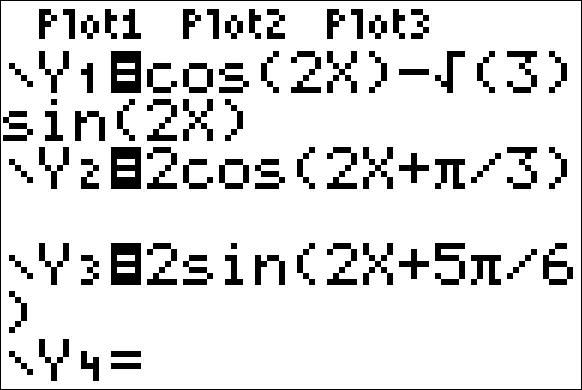
\includegraphics[width=2in]{./IntroTrigGraphics/TrigGraphs01.jpg} &

\hspace{0.75in} 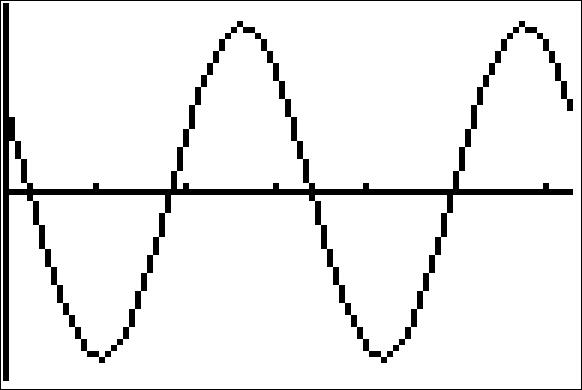
\includegraphics[width=2in]{./IntroTrigGraphics/TrigGraphs02.jpg} \\

\end{tabular}

\end{center}

\qed

\end{enumerate}

\end{ex}

It is important to note that in order for the technique presented in Example \ref{expandedsinusoidex1} to fit a function into one of the forms in Theorem \ref{sinusoidform},  the arguments of the cosine and sine function much match.  That is, while $f(x) = \cos(2x) - \sqrt{3} \sin(2x)$ is a sinusoid, $g(x) =  \cos(2x) - \sqrt{3} \sin(3x)$ is not.\footnote{This graph does, however, exhibit sinusoid-like characteristics!  Check it out!}  It is also worth mentioning that, had we chosen  $A = -2$ instead of $A = 2$ as we worked through Example \ref{expandedsinusoidex1}, our final answers would have \textit{looked} different. The reader is encouraged to rework Example  \ref{expandedsinusoidex1} using $A = -2$ to see what these differences are, and then for a challenging exercise, use identities to show that the formulas are all equivalent.  The general equations to fit a function of the form $f(x) = a \, \cos(\omega x) + b \, \sin(\omega x) + B$ into one of the forms in Theorem \ref{sinusoidform} are explored in Exercise \ref{sinusoidexercise1}.

\subsection{Graphs of the Secant and Cosecant Functions}
\label{secantcosecantgraphsection}

We now turn our attention to graphing $y = \sec(x)$.  Since $\sec(x) = \frac{1}{\cos(x)}$, we can use our table of values for the graph of $y = \cos(x)$ and take reciprocals. We know from Section \ref{circularfunctionsbeyond} that the domain of $F(x) = \sec(x)$ excludes all odd multiples of $\frac{\pi}{2}$, and sure enough, we run into trouble at $x = \frac{\pi}{2}$ and $x = \frac{3\pi}{2}$ since $\cos(x) = 0$ at these values.  Using the notation introduced in Section \ref{RationalGraphs}, we have that as $x \rightarrow \frac{\pi}{2}^{-}$, $\cos(x) \rightarrow 0^{+}$, so $\sec(x) \rightarrow \infty$. (See Section \ref{circularfunctionsbeyond} for a more detailed analysis.) Similarly, we find that  as $x \rightarrow \frac{\pi}{2}^{+}$, $\sec(x) \rightarrow -\infty$;  as $x \rightarrow \frac{3\pi}{2}^{-}$, $\sec(x) \rightarrow -\infty$; and as $x \rightarrow \frac{3\pi}{2}^{+}$, $\sec(x) \rightarrow \infty$.  This means we have a pair of vertical asymptotes to the graph of $y = \sec(x)$, $x = \frac{\pi}{2}$ and $x = \frac{3\pi}{2}$.  Since $\cos(x)$ is periodic with period $2\pi$, it follows that $\sec(x)$ is also.\footnote{Provided $\sec(\alpha)$ and  $\sec(\beta)$ are defined, $\sec(\alpha) = \sec(\beta)$ if and only if $\cos(\alpha) = \cos(\beta)$.  Hence, $\sec(x)$ inherits its period from $\cos(x)$.}  Below we graph a fundamental cycle of $y = \sec(x)$ \index{secant ! graph of} along with a more complete graph obtained by the usual `copying and pasting.'\footnote{In Section \ref{circularfunctionsbeyond}, we argued the range of $F(x) = \sec(x)$ is $(-\infty, -1] \cup [1,\infty)$.  We can now see this graphically.}

\hspace{.25in} \begin{tabular}{m{2.7in}m{3in}}
\setlength{\extrarowheight}{2pt}
\[ \begin{array}{|r||r|r|r|}  

\hline

 x & \cos(x) & \sec(x) & (x,\sec(x)) \\ \hline
0  & 1 & 1 & (0,1) \\ [2pt]   \hline
\frac{\pi}{4}  & \frac{\sqrt{2}}{2} & \sqrt{2} & \left(\frac{\pi}{4}, \sqrt{2} \right) \\ [2pt] \hline 
\frac{\pi}{2}  & 0 & \text{undefined} &  \\ [2pt] \hline 
\frac{3\pi}{4}  & -\frac{\sqrt{2}}{2} & -\sqrt{2} & \left(\frac{3\pi}{4}, -\sqrt{2} \right) \\ [2pt] \hline 
\pi & -1 & -1 &  (\pi, -1) \\ [2pt] \hline 
\frac{5\pi}{4}  & -\frac{\sqrt{2}}{2} & -\sqrt{2} & \left(\frac{5\pi}{4}, -\sqrt{2} \right) \\ [2pt] \hline 
\frac{3\pi}{2}  & 0 & \text{undefined} & \\ [2pt] \hline 
\frac{7\pi}{4}  & \frac{\sqrt{2}}{2} & \sqrt{2} & \left(\frac{7\pi}{4}, \sqrt{2} \right) \\ [2pt] \hline 
2\pi  & 1 &  1& (2\pi, 1) \\  [2pt] \hline
\end{array} \] \setlength{\extrarowheight}{0pt} &

\begin{mfpic}[25]{-1}{7}{-4}{4}
\point[3pt]{(0,1), (0.7854,1.4142),  (2.3562,-1.4142), (3.1416, -1), (3.9270,-1.4142),  (5.4978,1.4142), (6.2832,1)}
\axes
\tlabel[cc](7,-0.25){\scriptsize $x$}
\tlabel[cc](0.25,4){\scriptsize $y$}
\tcaption{The `fundamental cycle' of $y = \sec(x)$.}
\xmarks{0.7854, 1.5708, 2.3562, 3.1416, 3.9270, 4.7124,5.4978,6.2832 }
\ymarks{-3,-2,-1,1,2,3}
\tlpointsep{4pt}
\scriptsize
\axislabels {x}{{$\frac{\pi}{4}$} 0.7854, {$\frac{\pi}{2}$} 1.5708, {$\frac{3\pi}{4}$} 2.3562, {$\pi$} 3.1416, {$\frac{5\pi}{4}$} 3.9270, {$\frac{3\pi}{2}$} 4.7124, {$\frac{7\pi}{4}$} 5.4978, {$2\pi$} 6.2832}
\axislabels {y}{{$-3$} -3,{$-2$} -2,{$-1$} -1, {$1$} 1, {$2$} 2, {$3$} 3}
\normalsize
\dotted \function{0, 6.2832, 0.1}{cos(x)}
\dashed \polyline{(1.5708, -4), (1.5708, 4)}
\dashed \polyline{(4.7124, -4), (4.7124, 4)}
\arrow \function{0, 1.3181, 0.1}{1/cos(x)}
\arrow \reverse \arrow \function{1.8235, 4.460, 0.1}{1/cos(x)}
\arrow \reverse \function{4.9651, 6.28, 0.1}{1/cos(x)}
\end{mfpic} \\

\end{tabular}

\begin{center}

\begin{mfpic}[15]{-13}{13}{-4}{4}
\point[3pt]{(0,1), (3.1416, -1), (6.2832,1)}
\axes
\tlabel[cc](13,-0.25){\scriptsize $x$}
\tlabel[cc](0.25,4){\scriptsize $y$}
\tcaption{The graph of $y = \sec(x)$.}
\tlpointsep{4pt}
\dotted \function{-12.5664, 12.5664, 0.1}{cos(x)}
\dashed \polyline{(1.5708, -4), (1.5708, 4)}
\dashed \polyline{(4.7124, -4), (4.7124, 4)}
\dashed \polyline{(7.8540, -4), (7.8540, 4)}
\dashed \polyline{(10.9956, -4), (10.9956, 4)}
\dashed \polyline{(-1.5708, -4), (-1.5708, 4)}
\dashed \polyline{(-4.7124, -4), (-4.7124, 4)}
\dashed \polyline{(-7.8540, -4), (-7.8540, 4)}
\dashed \polyline{(-10.9956, -4), (-10.9956, 4)}
\arrow \reverse \arrow \function{-1.3181, 1.3181, 0.1}{1/cos(x)}
\arrow \reverse \arrow \function{1.8235, 4.460, 0.1}{1/cos(x)}
\arrow \reverse \arrow \function{4.9651, 7.6013, 0.1}{1/cos(x)}
\arrow \reverse \arrow \function{8.1067, 10.7432, 0.1}{1/cos(x)}
\arrow \reverse \arrow \function{-1.8235, -4.460, -0.1}{1/cos(x)}
\arrow \reverse \arrow \function{-4.9651, -7.6013, -0.1}{1/cos(x)}
\arrow \reverse \arrow \function{-8.1067, -10.7432, -0.1}{1/cos(x)}
\arrow \reverse \function{-11.2483, -12.5664, -0.1}{1/cos(x)}
\arrow \reverse \function{11.2483, 12.5664, 0.1}{1/cos(x)}
\penwd{1.5pt}
\arrow \function{0, 1.3181, 0.1}{1/cos(x)}
\arrow \reverse \arrow \function{1.8235, 4.460, 0.1}{1/cos(x)}
\arrow \reverse \function{4.9651, 6.28, 0.1}{1/cos(x)}
\end{mfpic}

\end{center}

As one would expect, to graph $y = \csc(x)$ we begin with $y = \sin(x)$ and take reciprocals of the corresponding $y$-values.  Here, we encounter issues at $x = 0$, $x = \pi$ and $x = 2\pi$.  Proceeding with the usual analysis, we graph the fundamental cycle of $y = \csc(x)$ below along with the dotted graph of $y=\sin(x)$ for reference.  Since $y = \sin(x)$ and $y = \cos(x)$ are merely phase shifts of each other, so too are $y = \csc(x)$ and $y = \sec(x)$. \index{cosecant ! graph of}

\hspace{.25in} \begin{tabular}{m{2.7in}m{3in}}
\setlength{\extrarowheight}{2pt}
\[ \begin{array}{|r||r|r|r|}  

\hline

 x & \sin(x) & \csc(x) & (x,\csc(x)) \\ \hline
0  & 0 & \text{undefined} &  \\ [2pt]   \hline
\frac{\pi}{4}  & \frac{\sqrt{2}}{2} & \sqrt{2} & \left(\frac{\pi}{4}, \sqrt{2} \right) \\ [2pt] \hline 
\frac{\pi}{2}  & 1 & 1 & \left(\frac{\pi}{2}, 1 \right) \\ [2pt] \hline 
\frac{3\pi}{4}  & \frac{\sqrt{2}}{2} & \sqrt{2} & \left(\frac{3\pi}{4}, \sqrt{2} \right) \\ [2pt] \hline 
\pi & 0 & \text{undefined} &   \\ [2pt] \hline 
\frac{5\pi}{4}  & -\frac{\sqrt{2}}{2} & -\sqrt{2} & \left(\frac{5\pi}{4}, -\sqrt{2} \right) \\ [2pt] \hline 
\frac{3\pi}{2}  & -1 & -1 & \left(\frac{3\pi}{2},-1 \right)\\ [2pt] \hline 
\frac{7\pi}{4}  & -\frac{\sqrt{2}}{2} & -\sqrt{2} & \left(\frac{7\pi}{4}, -\sqrt{2} \right) \\ [2pt] \hline 
2\pi  & 0 & \text{undefined} &  \\  [2pt] \hline
\end{array} \] \setlength{\extrarowheight}{0pt} &

\begin{mfpic}[25]{-1}{7}{-4}{4.25}
\point[3pt]{ (0.7854,1.4142), (1.5708, 1) ,(2.3562,1.4142), (4.7124, -1), (3.9270,-1.4142),  (5.4978,-1.4142)}
\axes
\tlabel[cc](7,-0.25){\scriptsize $x$}
\tlabel[cc](0.25,4.25){\scriptsize $y$}
\tcaption{The `fundamental cycle' of $y = \csc(x)$.}
\xmarks{0.7854, 1.5708, 2.3562, 3.1416, 3.9270, 4.7124,5.4978,6.2832 }
\ymarks{-3,-2,-1,1,2,3}
\tlpointsep{4pt}
\scriptsize 
\axislabels {x}{{$\frac{\pi}{4}$} 0.7854, {$\frac{\pi}{2}$} 1.5708, {$\frac{3\pi}{4}$} 2.3562, {$\pi$} 3.1416, {$\frac{5\pi}{4}$} 3.9270, {$\frac{3\pi}{2}$} 4.7124, {$\frac{7\pi}{4}$} 5.4978, {$2\pi$} 6.2832}
\axislabels {y}{{$-3$} -3,{$-2$} -2,{$-1$} -1, {$1$} 1, {$2$} 2, {$3$} 3}
\normalsize
\dotted \function{0, 6.2832, 0.1}{sin(x)}
\dashed \polyline{(3.1416, -4), (3.1416, 4)}
\dashed \polyline{(6.2832, -4), (6.2832, 4)}
\arrow \reverse \arrow \function{0.2527, 2.889, 0.1}{1/sin(x)}
\arrow \reverse \arrow \function{3.3943, 6.0306, 0.1}{1/sin(x)}
\end{mfpic} \\

\end{tabular}

Once again, our domain and range work in Section \ref{circularfunctionsbeyond} is verified geometrically in the graph of $y = G(x) = \csc(x)$.


\begin{center}

\begin{mfpic}[15]{-13}{13}{-4}{4.25}
\point[3pt]{ (1.5708, 1), (4.7124, -1)}
\axes
\tlabel[cc](13,-0.25){\scriptsize $x$}
\tlabel[cc](0.25,4.25){\scriptsize $y$}
\tcaption{The graph of $y = \csc(x)$.}
\tlpointsep{4pt}
\dotted \function{-12.5664, 12.5664, 0.1}{sin(x)}
\dashed \polyline{(3.1416, -4), (3.1416, 4)}
\dashed \polyline{(6.2832, -4), (6.2832, 4)}
\dashed \polyline{(-3.1416, -4), (-3.1416, 4)}
\dashed \polyline{(-6.2832, -4), (-6.2832, 4)}
\dashed \polyline{(9.4248, -4), (9.4248, 4)}
\dashed \polyline{(12.5664, -4), (12.5664, 4)}
\dashed \polyline{(-9.4248, -4), (-9.4248, 4)}
\dashed \polyline{(-12.5664, -4), (-12.5664, 4)}
\arrow \reverse \arrow \function{0.2527, 2.889, 0.1}{1/sin(x)}
\arrow \reverse \arrow \function{3.3943, 6.0306, 0.1}{1/sin(x)}
\arrow \reverse \arrow \function{-0.2527, -2.889, -0.1}{1/sin(x)}
\arrow \reverse \arrow \function{-3.3943, -6.0306, -0.1}{1/sin(x)}
\arrow \reverse \arrow \function{6.5359, 9.1723, 0.1}{1/sin(x)}
\arrow \reverse \arrow \function{-6.5359, -9.1723, -0.1}{1/sin(x)}
\arrow \reverse \arrow \function{9.6775, 12.3138, 0.1}{1/sin(x)}
\arrow \reverse \arrow \function{-9.6775, -12.3138, -0.1}{1/sin(x)}
\penwd{1.5pt}
\arrow \reverse \arrow \function{0.2527, 2.889, 0.1}{1/sin(x)}
\arrow \reverse \arrow \function{3.3943, 6.0306, 0.1}{1/sin(x)}
\end{mfpic}

\end{center}

Note that, on the intervals between the vertical asymptotes, both $F(x) = \sec(x)$ and $G(x) = \csc(x)$ are continuous and smooth.  In other words, they are continuous and smooth \textit{on their domains}.\footnote{Just like the rational functions in Chapter \ref{Rationals} are continuous and smooth on their domains because polynomials are continuous and smooth everywhere, the secant and cosecant functions are continuous and smooth on their domains since the cosine and sine functions are continuous and smooth everywhere.}  The following theorem summarizes the properties of the secant and cosecant functions.  Note that all of these properties are direct results of them being reciprocals of the cosine and sine functions, respectively.

\smallskip

\colorbox{ResultColor}{\bbm

\begin{thm} \label{secantcosecantfunctionprops}  \textbf{Properties of the Secant and Cosecant Functions} \index{secant ! properties of} \index{cosecant ! properties of}

\begin{itemize}

\item  The function $F(x) = \sec(x)$

\begin{itemize}


\item has domain $\left\{ x : x \neq \frac{\pi}{2} + \pi k, \, \,  \text{$k$ is an integer} \right\} = \displaystyle{\bigcup_{k=-\infty}^{\infty} \left(\frac{(2k+1) \pi}{2}, \frac{(2k+3) \pi}{2}\right)}$

\item has range $\{ y : |y| \geq 1 \} = (-\infty, -1] \cup [1, \infty)$

\item  is continuous and smooth on its domain

\item is even

\item has period $2\pi$

\end{itemize}

\item  The function $G(x) = \csc(x)$

\begin{itemize}

\item has domain $\left\{ x : x \neq \pi  k, \, \,  \text{$k$ is an integer} \right\} = \displaystyle{\bigcup_{k=-\infty}^{\infty}\left(k\pi, (k+1) \pi \right)}$

\item has range $\{ y : |y| \geq 1 \} = (-\infty, -1] \cup [1, \infty)$

\item  is continuous and smooth on its domain

\item is odd

\item has period $2\pi$

\end{itemize}

\end{itemize}

\end{thm}

\ebm}

\medskip

In the next example, we discuss graphing more general secant and cosecant curves.

\begin{ex}  \label{seccscgraphex} Graph one cycle of the following functions.  State the period of each.

\begin{multicols}{2}

\begin{enumerate}

\item  $f(x) = 1 - 2 \sec(2x)$

\item  $g(x) = \dfrac{\csc(\pi - \pi x) - 5}{3}$

\end{enumerate}

\end{multicols}

{\bf Solution.}  

\begin{enumerate}

\item  To graph $y = 1 - 2 \sec(2x)$, we follow the same procedure as in Example \ref{cosinesinegraphex1}.  First, we set the argument of secant, $2x$, equal to the `quarter marks' $0$, $\frac{\pi}{2}$, $\pi$, $\frac{3\pi}{2}$ and $2\pi$ and solve for $x$.

\setlength{\extrarowheight}{2pt}
\[ \begin{array}{|r|r|r|}  

\hline

 a & 2x = a & x \\ [2pt] \hline
0  & 2x = 0 & 0 \\ [2pt]   \hline

\frac{\pi}{2}  & 2x = \frac{\pi}{2} & \frac{\pi}{4} \\ [2pt] \hline 

\pi &  2x = \pi & \frac{\pi}{2} \\ [2pt] \hline 

\frac{3\pi}{2}  &  2x = \frac{3\pi}{2} & \frac{3\pi}{4} \\ [2pt] \hline 

2\pi  & 2x = 2\pi & \pi \\  [2pt] \hline
\end{array} \]
\setlength{\extrarowheight}{0pt}

Next, we substitute these $x$ values into $f(x)$.  If $f(x)$ exists, we have a point on the graph;  otherwise, we have found a vertical asymptote.  In addition to these points and asymptotes, we have graphed the associated cosine curve -- in this case $y = 1 - 2 \cos(2x)$ -- dotted in the picture below.  Since one cycle is graphed over the interval $[0,\pi]$, the period is $\pi - 0 = \pi$.
 

\hspace{.25in} \begin{tabular}{m{2.7in}m{3in}}
\setlength{\extrarowheight}{2pt}
\[ \begin{array}{|r||r|r|}  

\hline

 x & f(x) & (x,f(x))  \\ \hline
0  & - 1 & (0,-1)  \\ [2pt]   \hline
\frac{\pi}{4}  & \text{undefined} &  \\ [2pt] \hline 
\frac{\pi}{2}  & 3 & \left(\frac{\pi}{2}, 3 \right)  \\ [2pt] \hline 
\frac{3\pi}{4}  & \text{undefined} &  \\ [2pt] \hline 
\pi & -1 &   (\pi, -1) \\ [2pt] \hline 
\end{array} \] \setlength{\extrarowheight}{0pt} &

\begin{mfpic}[27][9]{-1}{4}{-7}{9}
\point[3pt]{(0,-1), (1.5708,3),  (3.1416, -1)}
\axes
\tlabel[cc](4,-0.3){\scriptsize $x$}
\tlabel[cc](0.25,9){\scriptsize $y$}
\tcaption{One cycle of $y = 1-2\sec(2x)$.}
\xmarks{0.7854, 1.5708, 2.3562, 3.1416}
\ymarks{-1,1,2,3}
\tlpointsep{4pt}
\scriptsize 
\axislabels {x}{{$\frac{\pi}{4}$} 0.7854, {$\frac{\pi}{2}$} 1.5708, {$\frac{3\pi}{4}$} 2.3562, {$\pi$} 3.1416}
\normalsize
\axislabels {y}{{\scriptsize $-1$} -1, {\scriptsize $1$} 1, {\scriptsize $2$} 2, {\scriptsize $3$} 3}
\dotted \function{0, 3.1416, 0.1}{1 - 2*cos(2*x)}
\dashed \polyline{(0.7854, -7), (0.7854, 9)}
\dashed \polyline{(2.3562, -7), (2.3562, 9)}
\arrow \function{0, 0.6590, 0.1}{1-2/cos(2*x)}
\arrow \reverse \arrow \function{0.9118, 2.230, 0.1}{1-2/cos(2*x)}
\arrow \reverse \function{2.4826, 3.14, 0.1}{1-2/cos(2*x)}
\end{mfpic} \\

\end{tabular}



\item  Proceeding as before, we set the argument of cosecant in $g(x) = \frac{\csc(\pi - \pi x) - 5}{3}$ equal to the quarter marks and solve for $x$.

\setlength{\extrarowheight}{2pt}
\[ \begin{array}{|r|r|r|}  

\hline

 a & \pi - \pi x = a & x \\ [2pt] \hline
0  & \pi - \pi x = 0 & 1 \\ [2pt]   \hline

\frac{\pi}{2}  & \pi - \pi x = \frac{\pi}{2} & \frac{1}{2} \\ [2pt] \hline 

\pi &  \pi - \pi x = \pi & 0 \\ [2pt] \hline 

\frac{3\pi}{2}  &  \pi - \pi x = \frac{3\pi}{2} & -\frac{1}{2} \\ [2pt] \hline 

2\pi  & \pi - \pi x = 2\pi & -1 \\  [2pt] \hline
\end{array} \]
\setlength{\extrarowheight}{0pt}

Substituting these $x$-values into $g(x)$, we generate the graph below and find the period to be $1 - (-1) = 2$.   The associated sine curve, $y = \frac{\sin(\pi - \pi x) - 5}{3}$, is dotted in as a reference.  

\hspace{.25in} \begin{tabular}{m{2.7in}m{3in}}
\setlength{\extrarowheight}{2pt}
\[ \begin{array}{|r||r|r|}  

\hline

 x & g(x) & (x,g(x))  \\ \hline
1  & \text{undefined} &   \\ [2pt]   \hline
\frac{1}{2}  & -\frac{4}{3} &  \left(\frac{1}{2}, -\frac{4}{3} \right)  \\ [2pt] \hline 
0 & \text{undefined} &   \\ [2pt] \hline 
-\frac{1}{2} & -2 & \left(-\frac{1}{2}, -2\right)  \\ [2pt] \hline 
-1 & \text{undefined} &    \\ [2pt] \hline 
\end{array} \] \setlength{\extrarowheight}{0pt} &

\begin{mfpic}[30]{-2}{2}{-3}{0.5}
\point[3pt]{(0.5,-1.3333),  (-0.5, -2)}
\axes
\tlabel[cc](2,-0.3){\scriptsize $x$}
\tlabel[cc](0.25,0.5){\scriptsize $y$}
\tcaption{One cycle of $y = \frac{\csc(\pi - \pi x) - 5}{3}$.}
\xmarks{-1, -0.5, 0.5, 1}
\ymarks{-2,-1}
\tlpointsep{4pt}
\axislabels {x}{{\scriptsize $-1 \hspace{7pt}$} -1, {\scriptsize $-\frac{1}{2} \hspace{7pt}$} -0.5, {\scriptsize $\frac{1}{2}$} 0.5, {\scriptsize $1$} 1}
\axislabels {y}{{\scriptsize $-2$} -2, {\scriptsize $-1$} -1}
\dotted \function{-1, 1, 0.1}{(sin(3.14159 - 3.14159*x)-5)/3}
\dashed \polyline{(-1, -3), (-1, -0.5)}
\dashed \polyline{(1, -3), (1,-0.5)}
\arrow \reverse \arrow \function{0.9196, 0.08040, -0.1}{((1/sin(3.14159 - 3.14159*x))-5)/3}
\arrow \reverse \arrow \function{-0.08043, -0.9196, 0.1}{((1/sin(3.14159 - 3.14159*x))-5)/3}
\end{mfpic} \\

\end{tabular}

\vspace{-0.2in}  \qed

\end{enumerate}

\end{ex}

Before moving on, we note that it is possible to speak of the period, phase shift and vertical shift of secant and cosecant graphs and use even/odd identities to put them in a form similar to the sinusoid forms mentioned in Theorem \ref{sinusoidform}.  Since these quantities match those of the corresponding cosine and sine curves, we do not spell this out explicitly.  Finally, since the ranges of secant and cosecant are unbounded, there is no amplitude associated with these curves.

\subsection{Graphs of the Tangent and Cotangent Functions}

Finally, we turn our attention to the graphs of the tangent and cotangent functions.  When constructing a table of values for the tangent function, we see that $J(x) = \tan(x)$ is undefined at $x  = \frac{\pi}{2}$ and $x = \frac{3\pi}{2}$, in accordance with our findings in Section \ref{circularfunctionsbeyond}.  As $x \rightarrow \frac{\pi}{2}^{-}$, $\sin(x) \rightarrow 1^{-}$ and $\cos(x) \rightarrow 0^{+}$, so that $\tan(x)  = \frac{\sin(x)}{\cos(x)}\rightarrow \infty$ producing a vertical asymptote at $x = \frac{\pi}{2}$.  Using a similar analysis, we get that as $x \rightarrow \frac{\pi}{2}^{+}$, $\tan(x) \rightarrow -\infty$; as $x \rightarrow \frac{3\pi}{2}^{-}$, $\tan(x) \rightarrow \infty$; and as $x \rightarrow \frac{3\pi}{2}^{+}$, $\tan(x) \rightarrow -\infty$.  Plotting this information and performing the usual `copy and paste' produces: \index{tangent ! graph of}


\hspace{.5in} \begin{tabular}{m{2.7in}m{3in}}
\setlength{\extrarowheight}{2pt}
\[ \begin{array}{|r||r|r|}  

\hline

 x & \tan(x) & (x,\tan(x)) \\ \hline
0  & 0 & (0, 0) \\ [2pt]   \hline
\frac{\pi}{4}  & 1 & \left(\frac{\pi}{4},1 \right) \\ [2pt] \hline 
\frac{\pi}{2}  & \text{undefined} &  \\ [2pt] \hline 
\frac{3\pi}{4}  & -1 & \left(\frac{3\pi}{4}, -1\right) \\ [2pt] \hline 
\pi & 0 & (\pi, 0) \\ [2pt] \hline 
\frac{5\pi}{4}  & 1 & \left(\frac{5\pi}{4}, 1 \right) \\ [2pt] \hline 
\frac{3\pi}{2}  & \text{undefined} &  \\ [2pt] \hline 
\frac{7\pi}{4}  & -1 & \left(\frac{7\pi}{4}, -1 \right) \\ [2pt] \hline 
2\pi  & 0 & (2\pi, 0) \\  [2pt] \hline
\end{array} \] \setlength{\extrarowheight}{0pt} &

\begin{mfpic}[25]{-1}{7}{-4}{4}
\point[3pt]{(0,0), (0.7854,1), (2.3562,-1), (3.1416, 0), (3.9270,1),  (5.4978,-1), (6.2832,0)}
\dashed \polyline{(1.5708,-4), (1.5708,4)}
\dashed \polyline{(4.7124,-4), (4.7124,4)}
\axes
\tlabel[cc](7,-0.25){\scriptsize $x$}
\tlabel[cc](0.25,4){\scriptsize $y$}
\tcaption{The graph of $y = \tan(x)$ over $[0,2\pi]$.}
\xmarks{0.7854, 1.5708, 2.3562, 3.1416, 3.9270, 4.7124,5.4978,6.2832 }
\ymarks{-1,1}
\tlpointsep{4pt}
\scriptsize
\axislabels {x}{{$\frac{\pi}{4}$} 0.7854, {$\frac{\pi}{2}$} 1.5708, {$\frac{3\pi}{4}$} 2.3562, {$\pi$} 3.1416, {$\frac{5\pi}{4}$} 3.9270, {$\frac{3\pi}{2}$} 4.7124, {$\frac{7\pi}{4}$} 5.4978, {$2\pi$} 6.2832}
\axislabels {y}{{$-1$} -1, {$1$} 1}
\normalsize
\arrow \function{0, 1.3258, 0.1}{tan(x)}
\arrow \reverse \arrow \function{1.8158, 4.4674, 0.1}{tan(x)}
\arrow \reverse \function{4.9574, 6.2832,0.1}{tan(x)}
\end{mfpic} \\

\end{tabular}



\begin{center}

\begin{mfpic}[15]{-13}{13}{-4}{4}
\point[3pt]{(-0.7854,-1), (0,0), (0.7854,1)}
\axes
\tlabel[cc](13,-0.25){\scriptsize $x$}
\tlabel[cc](0.25,4){\scriptsize $y$}
\tcaption{The graph of $y = \tan(x)$.}
\tlpointsep{4pt}
\dashed \polyline{(1.5708, -4), (1.5708, 4)}
\dashed \polyline{(4.7124, -4), (4.7124, 4)}
\dashed \polyline{(7.8540, -4), (7.8540, 4)}
\dashed \polyline{(10.9956, -4), (10.9956, 4)}
\dashed \polyline{(-1.5708, -4), (-1.5708, 4)}
\dashed \polyline{(-4.7124, -4), (-4.7124, 4)}
\dashed \polyline{(-7.8540, -4), (-7.8540, 4)}
\dashed \polyline{(-10.9956, -4), (-10.9956, 4)}
\arrow \reverse \arrow \function{-1.3181, 1.3181, 0.1}{tan(x)}
\arrow \reverse \arrow \function{1.8235, 4.460, 0.1}{tan(x)}
\arrow \reverse \arrow \function{4.9651, 7.6013, 0.1}{tan(x)}
\arrow \reverse \arrow \function{8.1067, 10.7432, 0.1}{tan(x)}
\arrow \reverse \arrow \function{-1.8235, -4.460, -0.1}{tan(x)}
\arrow \reverse \arrow \function{-4.9651, -7.6013, -0.1}{tan(x)}
\arrow \reverse \arrow \function{-8.1067, -10.7432, -0.1}{tan(x)}
\arrow \reverse \function{-11.2483, -12.5664, -0.1}{tan(x)}
\arrow \reverse \function{11.2483, 12.5664, 0.1}{tan(x)}
\penwd{1.5pt}
\arrow \reverse \arrow \function{-1.3181, 1.3181, 0.1}{tan(x)}
\end{mfpic}

\end{center}

From the graph, it appears as if the tangent function is periodic with period $\pi$.  To prove that this is the case, we appeal to the sum formula for tangents.  We have: \[ \tan(x+\pi) = \dfrac{\tan(x) + \tan(\pi)}{1 - \tan(x) \tan(\pi)} = \dfrac{\tan(x) + 0}{1 - (\tan(x) )(0)} = \tan(x),\]

which tells us the period of $\tan(x)$ is at most $\pi$.  To show that it is exactly $\pi$, suppose $p$ is a positive real number so that $\tan(x+p) = \tan(x)$ for all real numbers $x$.  For $x=0$, we have $\tan(p) = \tan(0+p) = \tan(0) = 0$, which means $p$ is a multiple of $\pi$.  The smallest positive multiple of $\pi$ is $\pi$ itself, so we have established the result.   We take as our fundamental cycle for $y=\tan(x)$ the interval $\left(-\frac{\pi}{2}, \frac{\pi}{2}\right)$, and use as our `quarter marks' $x = -\frac{\pi}{2}$, $-\frac{\pi}{4}$, $0$, $\frac{\pi}{4}$ and $\frac{\pi}{2}$. From the graph, we see confirmation of our domain and range work  in Section \ref{circularfunctionsbeyond}. 

\smallskip

It should be no surprise that $K(x) = \cot(x)$ behaves similarly to $J(x) = \tan(x)$. Plotting $\cot(x)$ over the interval $[0,2\pi]$ results in the graph below. \index{cotangent ! graph of}

\hspace{.5in} \begin{tabular}{m{2.7in}m{3in}}
\setlength{\extrarowheight}{2pt}
\[ \begin{array}{|r||r|r|}  

\hline

 x & \cot(x) & (x,\cot(x)) \\ \hline
0  & \text{undefined} &  \\ [2pt]   \hline
\frac{\pi}{4}  & 1 & \left(\frac{\pi}{4},1 \right) \\ [2pt] \hline 
\frac{\pi}{2}  & 0 & \left(\frac{\pi}{2},0 \right)  \\ [2pt] \hline 
\frac{3\pi}{4}  & -1 & \left(\frac{3\pi}{4}, -1\right) \\ [2pt] \hline 
\pi & \text{undefined} &  \\ [2pt] \hline 
\frac{5\pi}{4}  & 1 & \left(\frac{5\pi}{4}, 1 \right) \\ [2pt] \hline 
\frac{3\pi}{2}  & 0 & \left(\frac{3\pi}{2}, 0 \right) \\ [2pt] \hline 
\frac{7\pi}{4}  & -1 & \left(\frac{7\pi}{4}, -1 \right) \\ [2pt] \hline 
2\pi  & \text{undefined} &  \\  [2pt] \hline
\end{array} \] \setlength{\extrarowheight}{0pt} &

\begin{mfpic}[25]{-1}{7}{-4}{4.25}
\point[3pt]{ (0.7854,1), (1.5708,0), (2.3562,-1), (3.9270,1), (4.7124,0), (5.4978,-1)}
\dashed \polyline{(3.1416,-4), (3.1416,4)}
\dashed \polyline{(6.2832,-4), (6.2832,4)}
\axes
\tlabel[cc](7,-0.25){\scriptsize $x$}
\tlabel[cc](0.25,4.25){\scriptsize $y$}
\tcaption{The graph of $y = \cot(x)$ over $[0,2\pi]$.}
\xmarks{0.7854, 1.5708, 2.3562, 3.1416, 3.9270, 4.7124,5.4978,6.2832 }
\ymarks{-1,1}
\tlpointsep{4pt}
\scriptsize
\axislabels {x}{{$\frac{\pi}{4}$} 0.7854, {$\frac{\pi}{2}$} 1.5708, {$\frac{3\pi}{4}$} 2.3562, {$\pi$} 3.1416, {$\frac{5\pi}{4}$} 3.9270, {$\frac{3\pi}{2}$} 4.7124, {$\frac{7\pi}{4}$} 5.4978, {$2\pi$} 6.2832}
\axislabels {y}{{$-1$} -1, {$1$} 1}
\normalsize
\arrow \reverse \arrow \function{0.2450, 2.8966, 0.1}{cot(x)}
\arrow \reverse \arrow \function{3.3865, 6.0382,0.1}{cot(x)}
\end{mfpic} \\

\end{tabular}

From these data, it clearly appears as if the period of $\cot(x)$ is $\pi$, and we leave it to the reader to prove this.\footnote{Certainly, mimicking the proof that the period of $\tan(x)$ is an option;  for another approach, consider transforming $\tan(x)$ to $\cot(x)$ using identities.}  We take as one fundamental cycle the interval $(0,\pi)$ with quarter marks:  $x= 0$, $\frac{\pi}{4}$, $\frac{\pi}{2}$, $\frac{3\pi}{4}$ and $\pi$.  A more complete graph of $y=\cot(x)$ is below, along with the fundamental cycle highlighted as usual.  Once again, we see the domain and range of $K(x) = \cot(x)$ as read from the graph matches with what we found analytically in Section \ref{circularfunctionsbeyond}.     

\begin{center}

\begin{mfpic}[15]{-13}{13}{-4}{4.25}
\point[3pt]{ (0.7854,1), (1.5708,0), (2.3562,-1)}
\axes
\tlabel[cc](13,-0.25){\scriptsize $x$}
\tlabel[cc](0.25,4.25){\scriptsize $y$}
\tcaption{The graph of $y = \cot(x)$.}
\tlpointsep{4pt}
\dashed \polyline{(3.1416, -4), (3.1416, 4)}
\dashed \polyline{(6.2832, -4), (6.2832, 4)}
\dashed \polyline{(-3.1416, -4), (-3.1416, 4)}
\dashed \polyline{(-6.2832, -4), (-6.2832, 4)}
\dashed \polyline{(9.4248, -4), (9.4248, 4)}
\dashed \polyline{(12.5664, -4), (12.5664, 4)}
\dashed \polyline{(-9.4248, -4), (-9.4248, 4)}
\dashed \polyline{(-12.5664, -4), (-12.5664, 4)}
\arrow \reverse \arrow \function{0.2527, 2.889, 0.1}{cot(x)}
\arrow \reverse \arrow \function{3.3943, 6.0306, 0.1}{cot(x)}
\arrow \reverse \arrow \function{-0.2527, -2.889, -0.1}{cot(x)}
\arrow \reverse \arrow \function{-3.3943, -6.0306, -0.1}{cot(x)}
\arrow \reverse \arrow \function{6.5359, 9.1723, 0.1}{cot(x)}
\arrow \reverse \arrow \function{-6.5359, -9.1723, -0.1}{cot(x)}
\arrow \reverse \arrow \function{9.6775, 12.3138, 0.1}{cot(x)}
\arrow \reverse \arrow \function{-9.6775, -12.3138, -0.1}{cot(x)}
\penwd{1.5pt}
\arrow \reverse \arrow \function{0.2527, 2.889, 0.1}{cot(x)}
\end{mfpic}

\end{center}

The properties of the tangent and cotangent functions are summarized below. As with Theorem \ref{secantcosecantfunctionprops}, each of the results below can be traced back to properties of the cosine and sine functions and the definition of the tangent and cotangent functions as quotients thereof. 

\smallskip

\colorbox{ResultColor}{\bbm

\begin{thm} \label{tangentcotangentfunctionprops}  \textbf{Properties of the Tangent and Cotangent Functions} \index{tangent ! properties of} \index{cotangent ! properties of}

\begin{itemize}

\item  The function $J(x) = \tan(x)$

\begin{itemize}


\item has domain $\left\{ x : x \neq \frac{\pi}{2} + \pi k, \, \,  \text{$k$ is an integer} \right\} = \displaystyle{\bigcup_{k=-\infty}^{\infty} \left(\frac{(2k+1) \pi}{2}, \frac{(2k+3) \pi}{2}\right)}$

\item has range $(-\infty, \infty)$

\item is continuous and smooth on its domain

\item is odd

\item has period $\pi$

\end{itemize}

\item  The function $K(x) = \cot(x)$

\begin{itemize}

\item has domain $\left\{ x : x \neq \pi  k, \, \,  \text{$k$ is an integer} \right\} = \displaystyle{\bigcup_{k=-\infty}^{\infty}\left(k\pi, (k+1) \pi \right)}$

\item has range $(-\infty, \infty)$

\item is continuous and smooth on its domain

\item is odd

\item has period $\pi$

\end{itemize}

\end{itemize}

\end{thm}

\ebm}

\pagebreak

\begin{ex} \label{tancotgraphex} Graph one cycle of the following functions.  Find the period.

\begin{multicols}{2}

\begin{enumerate}

\item  $f(x) = 1 - \tan\left(\frac{x}{2}\right)$.

\item  $g(x) = 2\cot\left(\frac{\pi}{2} x + \pi\right) + 1$.

\end{enumerate}

\end{multicols}


{\bf Solution.}  

\begin{enumerate}

\item We proceed as we have in all of the previous graphing examples by setting the argument of tangent in $f(x) = 1 - \tan\left(\frac{x}{2}\right)$, namely $\frac{x}{2}$, equal to each of the `quarter marks' $-\frac{\pi}{2}$, $-\frac{\pi}{4}$, $0$, $\frac{\pi}{4}$ and $\frac{\pi}{2}$, and solving for $x$.

\setlength{\extrarowheight}{2pt}
\[ \begin{array}{|r|r|r|}  

\hline

 a & \frac{x}{2} = a & x \\ [2pt] \hline
-\frac{\pi}{2}  & \frac{x}{2} = -\frac{\pi}{2} & -\pi \\ [2pt]   \hline

-\frac{\pi}{4}  &\frac{x}{2} = -\frac{\pi}{4} & - \frac{\pi}{2} \\ [2pt] \hline 

0 &  \frac{x}{2} = 0 & 0 \\ [2pt] \hline 

\frac{\pi}{4}  &  \frac{x}{2} = \frac{\pi}{4} & \frac{\pi}{2} \\ [2pt] \hline 

\frac{\pi}{2}  & \frac{x}{2} = \frac{\pi}{2}  & \pi \\  [2pt] \hline
\end{array} \]
\setlength{\extrarowheight}{0pt}

Substituting these $x$-values into $f(x)$, we find points on the graph and the vertical asymptotes.

\hspace{.25in} \begin{tabular}{m{2.7in}m{3in}}
\setlength{\extrarowheight}{2pt}
\[ \begin{array}{|r||r|r|}  

\hline

 x & f(x) & (x,f(x))  \\ \hline
-\pi  & \text{undefined} &   \\ [2pt]   \hline
-\frac{\pi}{2}  &  2 &  \left(-\frac{\pi}{2}, 2 \right) \\ [2pt] \hline 
0 & 1 &  (0,1)  \\ [2pt] \hline 
\frac{\pi}{2}  & 0 &  \left(\frac{\pi}{2}, 0 \right) \\ [2pt] \hline 
\pi & \text{undefined} &  \\ [2pt] \hline 
\end{array} \] \setlength{\extrarowheight}{0pt} &

\begin{mfpic}[20]{-4}{4}{-3}{5}
\point[3pt]{(-1.5708,2),(0,1), (1.5708,0)}
\axes
\tlabel[cc](4,-0.3){\scriptsize $x$}
\tlabel[cc](0.25,5){\scriptsize $y$}
\tcaption{One cycle of $y = 1 - \tan\left(\frac{x}{2}\right)$.}
\xmarks{ -3.1416, -1.5708, 1.5708, 3.1416}
\ymarks{-2,-1,1,2}
\tlpointsep{4pt}
\scriptsize
\axislabels {x}{{$-\pi \hspace{7pt}$} -3.1416,{$-\frac{\pi}{2} \hspace{7pt}$} -1.5708, {$\frac{\pi}{2}$} 1.5708,, {$\pi$} 3.1416}
\normalsize
\axislabels {y}{{\scriptsize $-2$} -2,{\scriptsize $-1$} -1, {\scriptsize $1$} 1, {\scriptsize $2$} 2}
\dashed \polyline{(-3.1416, -3), (-3.1416, 5)}
\dashed \polyline{(3.1416, -3), (3.1416, 5)}
\arrow \reverse \arrow \function{-2.6516, 2.6516, 0.1}{1-tan(0.5*x)}
\end{mfpic} \\

\end{tabular}

We see that the period is $\pi - (-\pi) = 2\pi$.

\item  The `quarter marks' for the fundamental cycle of the cotangent curve are $0$, $\frac{\pi}{4}$, $\frac{\pi}{2}$, $\frac{3\pi}{4}$ and $\pi$.  To graph $g(x) = 2\cot\left(\frac{\pi}{2} x + \pi\right) + 1$, we begin by setting $\frac{\pi}{2} x + \pi$ equal to each quarter mark and solving for $x$.


\setlength{\extrarowheight}{2pt}
\[ \begin{array}{|r|r|r|}  

\hline

 a & \frac{\pi}{2} x + \pi = a & x \\ [2pt] \hline
0  & \frac{\pi}{2} x + \pi = 0 &  -2 \\ [2pt]   \hline

\frac{\pi}{4}  &  \frac{\pi}{2} x + \pi  = \frac{\pi}{4} & -\frac{3}{2} \\ [2pt] \hline 

\frac{\pi}{2}  &  \frac{\pi}{2} x + \pi = \frac{\pi}{2} & -1 \\ [2pt] \hline 

\frac{3\pi}{4}  &  \frac{\pi}{2} x + \pi =\frac{3\pi}{4} & -\frac{1}{2} \\ [2pt] \hline 

\pi  & \frac{\pi}{2} x + \pi = \pi   &  0 \\  [2pt] \hline
\end{array} \]
\setlength{\extrarowheight}{0pt}

We now use these $x$-values to generate our graph.

\hspace{.25in} \begin{tabular}{m{2.7in}m{3in}}
\setlength{\extrarowheight}{2pt}
\[ \begin{array}{|r||r|r|}  

\hline

 x & g(x) & (x,g(x))  \\ \hline
-2  & \text{undefined} &   \\ [2pt]   \hline
-\frac{3}{2}  &  3 &  \left(-\frac{3}{2}, 3 \right) \\ [2pt] \hline 
-1 & 1 &  (-1,1)  \\ [2pt] \hline 
-\frac{1}{2}  & -1 &  \left(-\frac{1}{2}, -1 \right) \\ [2pt] \hline 
0 & \text{undefined} &  \\ [2pt] \hline 
\end{array} \] \setlength{\extrarowheight}{0pt} &

\begin{mfpic}[30][20]{-3}{1}{-2}{4}
\point[3pt]{(-1.5,3),(-1,1), (-0.5,-1)}
\axes
\tlabel[cc](1,-0.3){\scriptsize $x$}
\tlabel[cc](0.25,4){\scriptsize $y$}
\tcaption{\scriptsize One cycle of $y = 2\cot\left(\frac{\pi}{2} x + \pi\right) + 1$.}
\xmarks{ -2, -1}
\ymarks{-1,1,2,3}
\tlpointsep{4pt}
\axislabels {x}{{\scriptsize $-2 \hspace{7pt}$} -2,{\scriptsize $-1 \hspace{7pt}$} -1}
\axislabels {y}{{\scriptsize $-1$} -1,{\scriptsize $1$} 1, {\scriptsize $2$} 2, {\scriptsize $3$} 3}
\dashed \polyline{(-2, -2), (-2, 4)}
\arrow \reverse \arrow \function{-1.62566, -0.3743, 0.1}{1+2*cot((1.5708*x)+ 3.1416)}
\end{mfpic} \\

\end{tabular}

We find the period to be $0 - (-2) = 2$. \qed

\end{enumerate}
\end{ex}

As with the secant and cosecant functions, it is possible to extend the notion of period, phase shift and vertical shift to the tangent and cotangent functions as we did for the cosine and sine functions in Theorem \ref{sinusoidform}.  Since the number of classical applications involving sinusoids far outnumber those involving tangent and cotangent functions, we omit this.  The ambitious reader is invited to formulate such a theorem, however.

\newpage

\subsection{Exercises}

In Exercises \ref{sinecosinegraphfirst} - \ref{sinecosinegraphlast}, graph one cycle of the given function.  State the period, amplitude, phase shift and vertical shift of the function.

\begin{multicols}{3}

\begin{enumerate}

\item $y = 3\sin(x)$ \label{sinecosinegraphfirst}
\item $y = \sin(3x)$
\item $y = -2\cos(x)$

\setcounter{HW}{\value{enumi}}

\end{enumerate}

\end{multicols}

\begin{multicols}{3}

\begin{enumerate}

\setcounter{enumi}{\value{HW}}

\item $y = \cos \left( x - \dfrac{\pi}{2} \right)$
\item $y = -\sin \left( x + \dfrac{\pi}{3} \right)$
\item $y = \sin(2x - \pi)$ \vphantom{$\left( \dfrac{\pi}{2} \right)$}

\setcounter{HW}{\value{enumi}}

\end{enumerate}

\end{multicols}

\begin{multicols}{3}

\begin{enumerate}

\setcounter{enumi}{\value{HW}}

\item $y = -\dfrac{1}{3}\cos \left( \dfrac{1}{2}x + \dfrac{\pi}{3} \right)$
\item $y = \cos (3x - 2\pi) + 4$ \vphantom{$\left( \dfrac{1\pi}{2} \right)$}
\item $y = \sin \left( -x - \dfrac{\pi}{4} \right) - 2$ \vphantom{$\left( \dfrac{1\pi}{2} \right)$}

\setcounter{HW}{\value{enumi}}

\end{enumerate}

\end{multicols}

\begin{multicols}{3}

\begin{enumerate}

\setcounter{enumi}{\value{HW}}

\item $y = \dfrac{2}{3} \cos \left( \dfrac{\pi}{2} - 4x \right) + 1$
\item $y = -\dfrac{3}{2} \cos \left( 2x + \dfrac{\pi}{3} \right) - \dfrac{1}{2}$
\item $y = 4\sin (-2\pi x + \pi)$ \vphantom{$\left( \dfrac{1\pi}{2} \right)$}  \label{sinecosinegraphlast}

\setcounter{HW}{\value{enumi}}

\end{enumerate}

\end{multicols}

In Exercises \ref{othergraphsfirst} - \ref{othergraphslast}, graph one cycle of the given function.  State the period of the function.

\begin{multicols}{3}

\begin{enumerate}

\setcounter{enumi}{\value{HW}}

\item $y = \tan \left(x - \dfrac{\pi}{3} \right)$ \vphantom{$\left( \dfrac{1\pi}{2} \right)$} \label{othergraphsfirst}
\item $y = 2\tan \left( \dfrac{1}{4}x \right) - 3$
\item $y = \dfrac{1}{3}\tan(-2x - \pi) + 1$

\setcounter{HW}{\value{enumi}}

\end{enumerate}

\end{multicols}

\begin{multicols}{3}

\begin{enumerate}

\setcounter{enumi}{\value{HW}}

\item $y = \sec \left( x - \dfrac{\pi}{2} \right)$ \vphantom{$\left( \dfrac{1\pi}{2} \right)$} 
\item $y = -\csc \left( x + \dfrac{\pi}{3} \right)$ \vphantom{$\left( \dfrac{1\pi}{2} \right)$} 
\item $y = -\dfrac{1}{3} \sec \left( \dfrac{1}{2}x + \dfrac{\pi}{3} \right)$

\setcounter{HW}{\value{enumi}}

\end{enumerate}

\end{multicols}

\begin{multicols}{3}

\begin{enumerate}

\setcounter{enumi}{\value{HW}}

\item $y = \csc (2x - \pi)$ \vphantom{$\left( \dfrac{\pi}{2} \right)$} 
\item $y = \sec(3x - 2\pi) + 4$ \vphantom{$\left( \dfrac{\pi}{2} \right)$} 
\item $y = \csc \left( -x - \dfrac{\pi}{4} \right) - 2$

\setcounter{HW}{\value{enumi}}

\end{enumerate}

\end{multicols}

\begin{multicols}{3}

\begin{enumerate}

\setcounter{enumi}{\value{HW}}

\item $y = \cot \left( x + \dfrac{\pi}{6} \right)$ \vphantom{$\left( \dfrac{1\pi}{2} \right)$} 
\item $y = -11\cot \left( \dfrac{1}{5} x \right)$
\item $y = \dfrac{1}{3} \cot \left( 2x + \dfrac{3\pi}{2} \right) + 1$ \label{othergraphslast}

\setcounter{HW}{\value{enumi}}

\end{enumerate}

\end{multicols}

In Exercises \ref{expandedsinusoidexerfirst} - \ref{expandedsinusoidexerlast}, use Example \ref{expandedsinusoidex1} as a guide to show that the function is a sinusoid by rewriting it in the forms $C(x) = A \cos(\omega x + \phi) + B$ and $S(x) = A \sin(\omega x + \phi) + B$ for $\omega > 0$ and $0 \leq \phi < 2\pi$.

\begin{multicols}{2}

\begin{enumerate}

\setcounter{enumi}{\value{HW}}

\item $f(x) = \sqrt{2}\sin(x) + \sqrt{2}\cos(x) + 1$ \label{expandedsinusoidexerfirst}
\item $f(x) = 3\sqrt{3}\sin(3x) - 3\cos(3x)$

\setcounter{HW}{\value{enumi}}

\end{enumerate}

\end{multicols}

\begin{multicols}{2}

\begin{enumerate}

\setcounter{enumi}{\value{HW}}

\item $f(x) = -\sin(x) + \cos(x) - 2$ \vphantom{$\left( -\dfrac{1\sqrt{3}}{2} \right)$} 
\item $f(x) = -\dfrac{1}{2}\sin(2x) - \dfrac{\sqrt{3}}{2}\cos(2x)$

\setcounter{HW}{\value{enumi}}

\end{enumerate}

\end{multicols}

\begin{multicols}{2}

\begin{enumerate}

\setcounter{enumi}{\value{HW}}

\item  $f(x) = 2\sqrt{3} \cos(x) - 2\sin(x)$ \vphantom{$\left( -\dfrac{3\sqrt{3}}{2} \right)$} 
\item  $f(x) = \dfrac{3}{2} \cos(2x) - \dfrac{3\sqrt{3}}{2} \sin(2x) + 6$

\setcounter{HW}{\value{enumi}}

\end{enumerate}

\end{multicols}

\begin{multicols}{2}

\begin{enumerate}

\setcounter{enumi}{\value{HW}}

\item  $f(x) = -\dfrac{1}{2} \cos(5x) -\dfrac{\sqrt{3}}{2} \sin(5x)$
\item  $f(x) = -6\sqrt{3} \cos(3x) - 6\sin(3x) - 3$ \vphantom{$\left( -\dfrac{\sqrt{3}}{2} \right)$} 

\setcounter{HW}{\value{enumi}}

\end{enumerate}

\end{multicols}

\begin{multicols}{2}

\begin{enumerate}

\setcounter{enumi}{\value{HW}}

\item  $f(x) =  \dfrac{5\sqrt{2}}{2} \sin(x)  -\dfrac{5\sqrt{2}}{2} \cos(x)$
\item  $f(x) =3 \sin \left(\dfrac{x}{6}\right) -3\sqrt{3} \cos \left(\dfrac{x}{6}\right)$ \vphantom{$\left( \dfrac{-5 \sqrt{3}}{2} \right)$}  \label{expandedsinusoidexerlast}

\setcounter{HW}{\value{enumi}}

\end{enumerate}

\end{multicols}

\begin{enumerate}

\setcounter{enumi}{\value{HW}}

\item In Exercises \ref{expandedsinusoidexerfirst} - \ref{expandedsinusoidexerlast}, you should have noticed a relationship between the phases $\phi$ for the $S(x)$ and $C(x)$.  Show that if $f(x) = A \sin(\omega x + \alpha) + B$, then $f(x) = A \cos(\omega x + \beta) + B$ where $\beta = \alpha - \dfrac{\pi}{2}$. 
\label{sinusoidexercise1}

\item Let $\phi$ be an angle measured in radians and let $P(a,b)$ be a point on the terminal side of $\phi$ when it is drawn in standard position.  Use Theorem \ref{cosinesinecircle} and the sum identity for sine in Theorem \ref{sinesumdifference} to show that  $f(x) = a \, \sin(\omega x) + b\, \cos(\omega x) + B$ (with  $\omega > 0$) can be rewritten as $f(x) = \sqrt{a^{2} + b^{2}}\sin(\omega x + \phi) + B$.
\label{sinusoidexercise2}

\item  With the help of your classmates, express the domains of the functions in Examples \ref{seccscgraphex} and \ref{tancotgraphex} using extended interval notation. (We will revisit this in Section \ref{TrigEquIneq}.)  

\setcounter{HW}{\value{enumi}}

\end{enumerate}

In Exercises \ref{idengraphfirst} - \ref{idengraphlast}, verify the identity by graphing the right and left hand sides on a calculator.

\begin{multicols}{3}

\begin{enumerate}

\setcounter{enumi}{\value{HW}}

\item $\sin^{2}(x) + \cos^{2}(x) = 1$ \vphantom{$\left( \dfrac{\pi}{2} \right)$} \label{idengraphfirst} 
\item $\sec^{2}(x) - \tan^{2}(x) = 1$ \vphantom{$\left( \dfrac{\pi}{2} \right)$}
\item  $\cos(x) = \sin\left(\dfrac{\pi}{2} - x\right)$

\setcounter{HW}{\value{enumi}}

\end{enumerate}

\end{multicols}

\begin{multicols}{3}

\begin{enumerate}

\setcounter{enumi}{\value{HW}}

\item  $\tan(x+\pi) = \tan(x)$ \vphantom{$\dfrac{\sin(x)}{1+\cos(x)}$}
\item  $\sin(2x) = 2\sin(x)\cos(x)$ \vphantom{$\dfrac{\sin(x)}{1+\cos(x)}$}
\item  $\tan\left(\dfrac{x}{2}\right) = \dfrac{\sin(x)}{1+\cos(x)}$ \label{idengraphlast}

\setcounter{HW}{\value{enumi}}

\end{enumerate}

\end{multicols}

In Exercises \ref{exploregraphsfirst} - \ref{exploregraphslast}, graph the function with the help of your calculator and discuss the given questions with your classmates.

\begin{enumerate}

\setcounter{enumi}{\value{HW}}

\item  $f(x) = \cos(3x) + \sin(x)$.  Is this function periodic?  If so, what is the period? \label{exploregraphsfirst}
\item  $f(x) = \frac{\sin(x)}{x}$.  What appears to be the horizontal asymptote of the graph? 
\item  $f(x) = x \sin(x)$.  Graph $y = \pm x$ on the same set of axes and describe the behavior of $f$. 
\item  $f(x) = \sin\left(\frac{1}{x}\right)$.  What's happening as $x \rightarrow 0$?
\item  $f(x) = x - \tan(x)$.  Graph $y = x$ on the same set of axes and describe the behavior of $f$.  
\item  $f(x) = e^{-0.1x} \left( \cos(2x) + \sin(2x)\right)$.  Graph $y = \pm e^{-0.1x}$ on the same set of axes and  describe the behavior of $f$.
\item  $f(x) = e^{-0.1x} \left( \cos(2x) + 2\sin(x)\right)$.  Graph $y = \pm e^{-0.1x}$ on the same set of axes and  describe the behavior of $f$. \label{exploregraphslast}

\setcounter{HW}{\value{enumi}}

\end{enumerate}

\begin{enumerate}

\setcounter{enumi}{\value{HW}}

\item Show that a constant function $f$ is periodic by showing that $f(x + 117) = f(x)$ for all real numbers $x$. Then show that $f$ has no period by showing that you cannot find a \emph{smallest} number $p$ such that $f(x + p) = f(x)$ for all real numbers $x$.  Said another way, show that $f(x + p) = f(x)$ for all real numbers $x$ for ALL values of $p > 0$, so no smallest value exists to satisfy the definition of `period'.

\setcounter{HW}{\value{enumi}}

\end{enumerate}

\newpage

\subsection{Answers}

\begin{enumerate}

\item \begin{multicols}{2} \raggedcolumns
$y = 3\sin(x)$\\
Period: $2\pi$\\
Amplitude: $3$\\
Phase Shift: $0$\\
Vertical Shift: $0$\\

\begin{mfpic}[25][15]{-0.25}{7}{-3.5}{3.75}
\point[3pt]{(0,0), (1.5708,3), (3.1416, 0), (4.7124,-3), (6.2832,0)}
\axes
\tlabel[cc](7,-0.30){$x$}
\tlabel[cc](0.25,3.75){$y$}
\xmarks{1.5708, 3.1416, 4.7124, 6.2832 }
\ymarks{-3,3}
\tlpointsep{4pt}
\axislabels {x}{{$\frac{\pi}{2}$} 1.5708, {$\pi$} 3.1416, {$\frac{3\pi}{2}$} 4.7124, {$2\pi$} 6.2832}
\axislabels {y}{{$-3$} -3, {$3$} 3}
\function{0, 6.2832, 0.1}{3*sin(x)}
\end{mfpic}

\end{multicols}

\item \begin{multicols}{2} \raggedcolumns
$y = \sin(3x)$\\
Period: $\dfrac{2\pi}{3}$\\
Amplitude: $1$\\
Phase Shift: $0$\\
Vertical Shift: $0$\\

\begin{mfpic}[70][50]{-0.25}{2.5}{-1.25}{1.25}
\point[3pt]{(0,0), (0.5236,1), (1.0472,0), (1.5708,-1), (2.0944,0)}
\axes
\tlabel[cc](2.5,-0.15){$x$}
\tlabel[cc](0.15,1.25){$y$}
\xmarks{0.5236, 1.0472, 1.5708, 2.0944}
\ymarks{-1,1}
\tlpointsep{4pt}
\axislabels {x}{{$\frac{\pi}{6}$} 0.5236, {$\frac{\pi}{3}$} 1.0472, {$\frac{\pi}{2}$} 1.5708, {$\frac{2\pi}{3}$} 2.0944}
\axislabels {y}{{$-1$} -1, {$1$} 1}
\function{0, 2.0944, 0.1}{sin(3*x)}
\end{mfpic}

\end{multicols}

\item \begin{multicols}{2} \raggedcolumns
$y = -2\cos(x)$\\
Period: $2\pi$\\
Amplitude: $2$\\
Phase Shift: $0$\\
Vertical Shift: $0$\\

\begin{mfpic}[25]{-0.25}{7}{-2.5}{2.5}
\point[3pt]{(0,-2), (1.5708,0), (3.1416, 2), (4.7124,0), (6.2832,-2)}
\axes
\tlabel[cc](7,-0.25){$x$}
\tlabel[cc](0.25,2.5){$y$}
\xmarks{1.5708, 3.1416, 4.7124, 6.2832}
\ymarks{-2,2}
\tlpointsep{4pt}
\axislabels {x}{{$\frac{\pi}{2}$} 1.5708, {$\pi$} 3.1416, {$\frac{3\pi}{2}$} 4.7124, {$2\pi$} 6.2832}
\axislabels {y}{{$-2$} -2, {$2$} 2}
\function{0, 6.2832, 0.1}{-2*cos(x)}
\end{mfpic}

\end{multicols}

\item \begin{multicols}{2} \raggedcolumns
$y = \cos \left( x - \dfrac{\pi}{2} \right)$\\
Period: $2\pi$\\
Amplitude: $1$\\
Phase Shift: $\dfrac{\pi}{2}$\\
Vertical Shift: $0$\\

\begin{mfpic}[22][40]{-0.25}{8.3}{-1.5}{1.5}
\point[3pt]{(1.5708,1), (3.1416, 0), (4.7124,-1), (6.2832,0), (7.854,1)}
\axes
\tlabel[cc](8.3,-0.25){$x$}
\tlabel[cc](0.25,1.5){$y$}
\xmarks{1.5708, 3.1416, 4.7124, 6.2832, 7.854}
\ymarks{-1,1}
\tlpointsep{4pt}
\axislabels {x}{{$\frac{\pi}{2}$} 1.5708, {$\pi$} 3.1416, {$\frac{3\pi}{2}$} 4.7124, {$2\pi$} 6.2832, {$\frac{5\pi}{2}$} 7.854}
\axislabels {y}{{$-1$} -1, {$1$} 1}
\function{1.5708, 7.854, 0.1}{cos(x - 1.5708)}
\end{mfpic}

\end{multicols}


\item \begin{multicols}{2} \raggedcolumns
$y = -\sin \left( x + \dfrac{\pi}{3} \right)$\\
Period: $2\pi$\\
Amplitude: $1$\\
Phase Shift: $-\dfrac{\pi}{3}$\\
Vertical Shift: $0$\\

\begin{mfpic}[27][40]{-1.25}{5.75}{-1.5}{1.5}
\point[3pt]{(-1.0472,0), (0.5236,-1), (2.0944,0), (3.6652,1), (5.236,0)}
\axes
\tlabel[cc](5.75,-0.25){$x$}
\tlabel[cc](0.25,1.5){$y$}
\xmarks{-1.0472, 0.5236, 2.0944, 3.6652, 5.236}
\ymarks{-1,1}
\tlpointsep{4pt}
\axislabels {x}{{$-\frac{\pi}{3}$} -1.0472, {$\frac{\pi}{6}$} 0.5236, {$\frac{2\pi}{3}$} 2.0944, {$\frac{7\pi}{6}$} 3.6652, {$\frac{5\pi}{3}$} 5.236}
\axislabels {y}{{$-1$} -1, {$1$} 1}
\function{-1.0472, 5.236, 0.1}{-sin(x + 1.0472)}
\end{mfpic}

\end{multicols}

\item \begin{multicols}{2} \raggedcolumns
$y = \sin(2x - \pi)$\\
Period: $\pi$\\
Amplitude: $1$\\
Phase Shift: $\dfrac{\pi}{2}$\\
Vertical Shift: $0$\\

\begin{mfpic}[35][50]{0}{5.25}{-1.15}{1.5}
\point[3pt]{(1.5708,0), (2.3562,1), (3.1415,0), (3.927,-1), (4.7124,0)}
\axes
\tlabel[cc](5.25,-0.25){$x$}
\tlabel[cc](0.25,1.5){$y$}
\xmarks{1.5708, 2.3562, 3.1415, 3.927, 4.7124}
\ymarks{-1,1}
\tlpointsep{4pt}
\axislabels {x}{{$\frac{\pi}{2}$} 1.5708, {$\frac{3\pi}{4}$} 2.3562, {$\pi$} 3.1415, {$\frac{5\pi}{4}$} 3.927, {$\frac{3\pi}{2}$} 4.7124}
\axislabels {y}{{$-1$} -1, {$1$} 1}
\function{1.5708, 4.7124, 0.1}{sin(2*x - 3.1415)}
\end{mfpic}

\end{multicols}

\item \begin{multicols}{2} \raggedcolumns
$y = -\dfrac{1}{3}\cos \left( \dfrac{1}{2}x + \dfrac{\pi}{3} \right)$\\
Period: $4\pi$\\
Amplitude: $\dfrac{1}{3}$\\
Phase Shift: $-\dfrac{2\pi}{3}$\\
Vertical Shift: $0$\\

\begin{mfpic}[14][100]{-2.25}{11.5}{-0.5}{0.5}
\point[3pt]{(-2.0944, -0.3333), (1.0472, 0), (4.1888, 0.3333), (7.3304, 0), (10.472, -0.3333)}
\axes
\tlabel[cc](11.5,-0.05){$x$}
\tlabel[cc](0.25,0.5){$y$}
\xmarks{-2.0944, 1.0472, 4.1888, 7.3304, 10.472}
\ymarks{-0.3333, 0.3333}
\tlpointsep{4pt}
\axislabels {x}{{$-\frac{2\pi}{3}$} -2.0944, {$\frac{\pi}{3}$} 1.0472, {$\frac{4\pi}{3}$} 4.1888, {$\frac{7\pi}{3}$} 7.3304, {$\frac{10\pi}{3}$} 10.472}
\axislabels {y}{{$-\frac{1}{3}$} -0.3333, {$\frac{1}{3}$} 0.3333}
\function{-2.0944, 10.472, 0.1}{-0.3333*cos(0.5*x + 1.0472)}
\end{mfpic}

\end{multicols}

\item \begin{multicols}{2} \raggedcolumns
$y = \cos (3x - 2\pi) + 4$\\
Period: $\dfrac{2\pi}{3}$\\
Amplitude: $1$\\
Phase Shift:  $\dfrac{2\pi}{3}$\\
Vertical Shift: 4\\

\begin{mfpic}[36][25]{-0.5}{5}{-0.5}{5.5}
\point[3pt]{(2.0944,5), (2.618,4), (3.1415,3), (3.6652,4), (4.1888,5)}
\axes
\tlabel[cc](5,-0.25){$x$}
\tlabel[cc](0.25,5.5){$y$}
\xmarks{2.0944, 2.618, 3.1415, 3.6652, 4.1888}
\ymarks{3,4,5}
\tlpointsep{4pt}
\axislabels {x}{{$\frac{2\pi}{3}$} 2.0944, {$\frac{5\pi}{6}$} 2.618, {$\pi$} 3.1415, {$\frac{7\pi}{6}$} 3.6652, {$\frac{4\pi}{3}$} 4.1888}
\axislabels {y}{{$3$} 3, {$4$} 4, {$5$} 5}
\function{2.0944, 4.1888, 0.1}{cos(3*x - 6.2834) + 4}
\end{mfpic}

\end{multicols}

\item \begin{multicols}{2} \raggedcolumns
$y = \sin \left( -x - \dfrac{\pi}{4} \right) - 2$ \\
Period: $2\pi$\\
Amplitude: $1$\\
Phase Shift: $-\dfrac{\pi}{4}$ (You need to use \\ \vspace*{.1in}
$y = -\sin \left( x + \dfrac{\pi}{4} \right) - 2 $ to find this.)\footnote{Two cycles of the graph are shown to illustrate the discrepancy discussed on page \pageref{phaseshiftissue}.}\\
Vertical Shift: $-2$\\

\begin{mfpic}[13][27]{-7.5}{6.5}{-3.25}{0.5}
\point[3pt]{(-7.0686,-2), (-5.4979,-3), (-3.927,-2), (-2.3562,-1), (-0.7854,-2), (0.7854,-3), (2.3562,-2), (3.927,-1), (5.4979,-2)}
\axes
\tlabel[cc](6.5,-0.25){$x$}
\tlabel[cc](0.25,0.5){$y$}
\xmarks{-7.0686, -5.4979, -3.927, -2.3562,-0.7854, 0.7854, 2.3562, 3.927, 5.4979}
\ymarks{-3,-2,-1}
\tlpointsep{5pt}
\axislabels {x}{{$-\frac{9\pi}{4} \hspace{6pt}$} -7.0686, {$-\frac{7\pi}{4} \hspace{6pt}$} -5.4979, {$-\frac{5\pi}{4} \hspace{6pt}$} -3.927, {$-\frac{3\pi}{4} \hspace{6pt}$} -2.3562, {$-\frac{\pi}{4} \hspace{6pt}$} -0.7854, {$\frac{\pi}{4}$} 0.7854, {$\frac{3\pi}{4}$} 2.3562, {$\frac{5\pi}{4}$} 3.927, {$\frac{7\pi}{4}$} 5.4979}
\axislabels {y}{{$-3$} -3, {$-2$} -2, {$-1$} -1}
\function{-7.0686, 5.4979, 0.1}{-1*sin(x + 0.7854) - 2}
\end{mfpic}

\end{multicols}

\item \begin{multicols}{2} \raggedcolumns
$y = \dfrac{2}{3} \cos \left( \dfrac{\pi}{2} - 4x \right) + 1$\\ 
Period: $\dfrac{\pi}{2}$\\
Amplitude: $\dfrac{2}{3}$\\ 
Phase Shift: $\dfrac{\pi}{8}$ (You need to use \\
$y = \dfrac{2}{3} \cos \left( 4x - \dfrac{\pi}{2} \right) + 1$ to find this.)\footnote{Again, we graph two cycles to illustrate the discrepancy discussed on page \pageref{phaseshiftissue}.}\\
Vertical Shift: $1$\\

\begin{mfpic}[52][45]{-1.5}{2.25}{-0.25}{2}
\point[3pt]{(-1.1781, 1.6667), (-0.7854, 1), (-0.3927, 0.3333), (0, 1), (0.3927, 1.6667), (0.7854, 1), (1.1781, 0.3333), (1.5708, 1), (1.9635, 1.6667)}
\axes
\tlabel[cc](2.25,-0.25){$x$}
\tlabel[cc](0.15,2){$y$}
\xmarks{-1.1781, -0.7854, -0.3927, 0.3927, 0.7854, 1.1781, 1.5708, 1.9635}
\ymarks{0.3333, 1, 1.6667}
\tlpointsep{4pt}
\axislabels {x}{{$-\frac{3\pi}{8} \hspace{6pt}$} -1.1781, {$-\frac{\pi}{4} \hspace{6pt}$} -0.7854, {$-\frac{\pi}{8} \hspace{6pt}$} -0.3927, {$\frac{\pi}{8}$} 0.3927, {$\frac{\pi}{4}$} 0.7854, {$\frac{3\pi}{8}$} 1.1781, {$\frac{\pi}{2}$} 1.5708, {$\frac{5\pi}{8}$} 1.9635}
\axislabels {y}{{$\frac{1}{3}$} 0.333, {$1$} 1, {$\frac{5}{3}$} 1.6667}
\function{-1.1781, 1.9635, 0.1}{0.6667*cos(4*x - 1.5708) + 1}
\end{mfpic}

\end{multicols}

\item \begin{multicols}{2} \raggedcolumns
$y = -\dfrac{3}{2} \cos \left( 2x + \dfrac{\pi}{3} \right) - \dfrac{1}{2}$\\
Period: $\pi$\\
Amplitude: $\dfrac{3}{2}$\\
Phase Shift: $-\dfrac{\pi}{6}$\\
Vertical Shift: $-\dfrac{1}{2}$\\

\begin{mfpic}[51][30]{-.75}{3}{-2.25}{1.5}
\point[3pt]{(-0.5236,-2), (0.2618,-0.5), (1.0472, 1), (1.8326, -0.5), (2.618, -2)}
\axes
\tlabel[cc](3,-0.25){$x$}
\tlabel[cc](0.15,1.5){$y$}
\xmarks{-0.5236, 0.2618, 1.0472, 1.8326, 2.618}
\ymarks{-2, -0.5, 1}
\tlpointsep{4pt}
\axislabels {x}{{$-\frac{\pi}{6}$} -0.5236, {$\frac{\pi}{12}$} 0.2618, {$\frac{\pi}{3}$} 1.0472, {$\frac{7\pi}{12}$} 1.8326, {$\frac{5\pi}{6}$} 2.618}
\axislabels {y}{{$-2$} -2, {$-\frac{1}{2}$} -0.5, {$1$} 1}
\function{-0.5236, 2.618, 0.1}{-1.5*cos(2*x + 1.047) - 0.5}
\end{mfpic}

\end{multicols}

\item \begin{multicols}{2} \raggedcolumns
$y = 4\sin (-2\pi x + \pi)$ \\
Period: $1$\\
Amplitude: $4$\\
Phase Shift: $\dfrac{1}{2}$ (You need to use \\
$y =  -4\sin (2\pi x - \pi)$ to find this.)\footnote{This will be the last time we graph two cycles to illustrate the discrepancy discussed on page \pageref{phaseshiftissue}.}\\
Vertical Shift: $0$\\

\begin{mfpic}[80][12]{-.75}{1.75}{-4.5}{4.75}
\point[3pt]{(-0.5,0), (-0.25,-4), (0,0), (0.25,4), (0.5,0), (0.75,-4), (1,0), (1.25,4), (1.5,0)}
\axes
\tlabel[cc](1.75,-0.5){$x$}
\tlabel[cc](0.1,4.75){$y$}
\xmarks{-0.5, -0.25, 0.25, 0.5, 0.75, 1, 1.25, 1.5}
\ymarks{-4,4}
\tlpointsep{4pt}
\axislabels {x}{{$-\frac{1}{2}$ \hspace{6pt}} -0.5, {$-\frac{1}{4}$ \hspace{6pt}} -0.25, {$\frac{1}{4}$} 0.25, {$\frac{1}{2}$} 0.5, {$\frac{3}{4}$} 0.75, {$1$} 1, {$\frac{5}{4}$} 1.25, {$\frac{3}{2}$} 1.5}
\axislabels {y}{{$-4$} -4, {$4$} 4}
\function{-0.5, 1.5, 0.01}{(-4)*sin((6.2831853*x) - 3.14159265)}
\end{mfpic}

\end{multicols}

\setcounter{HW}{\value{enumi}}
\end{enumerate}

\begin{enumerate}

\setcounter{enumi}{\value{HW}}

\item \begin{multicols}{2} \raggedcolumns
$y = \tan \left(x - \dfrac{\pi}{3} \right)$\\
Period: $\pi$\\

\begin{mfpic}[46][18]{-1}{3}{-5}{5}
\point[3pt]{(0.2618,-1), (1.0472,0), (1.8326,1)}
\axes
\tlabel[cc](3,-0.5){$x$}
\tlabel[cc](0.25,5){$y$}
\xmarks{0.2618, 1.0472, 1.8326}
\ymarks{-1,1}
\tlpointsep{4pt}
\axislabels {x}{{$-\frac{\pi}{6}$ \hspace{11pt}} -0.5236, {$\frac{\pi}{12}$} 0.2618, {$\frac{\pi}{3}$} 1.0472, {$\frac{7\pi}{12}$} 1.8326, {$\frac{5\pi}{6}$ \hspace{11pt}} 2.618}
\axislabels {y}{{$-1$} -1, {$1$} 1}
\arrow \reverse \arrow \function{-0.30, 2.40, 0.1}{tan(x - 1.0472)}
\dashed \polyline{(-0.5236,-5), (-0.5236,5)}
\dashed \polyline{(2.618,-5),(2.618,5)}
\end{mfpic}

\end{multicols}

\item \begin{multicols}{2} \raggedcolumns
$y = 2\tan \left( \dfrac{1}{4}x \right) - 3$\\
Period: $4\pi$

\begin{mfpic}[13][13]{-7}{8}{-10}{4}
\point[3pt]{(-3.1416,-5), (0,-3), (3.1416,-1)}
\axes
\tlabel[cc](8,-0.5){$x$}
\tlabel[cc](0.5,4){$y$}
\xmarks{-3.1416, 3.1416}
\ymarks{-5, -3, -1}
\tlpointsep{4pt}
\axislabels {x}{{$-2\pi$} -6.2832, {$-\pi$ \hspace{6pt}} -3.1416, {$\pi$} 3.1416, {\hspace{11pt}$2\pi$} 6.2832}
\axislabels {y}{{$-5$} -5, {$-3$} -3, {$-1$} -1}
\arrow \reverse \arrow \function{-5.1, 5.1, 0.1}{2*tan(0.25*x) - 3}
\dashed \polyline{(-6.2832,-10), (-6.2832,4)}
\dashed \polyline{(6.2382,-10),(6.2832,4)}
\end{mfpic}

\end{multicols}

\item \begin{multicols}{2} \raggedcolumns
$y = \dfrac{1}{3}\tan(-2x - \pi) + 1$ \\
is equivalent to \\
$y = -\dfrac{1}{3}\tan(2x + \pi) + 1$ \\
via the Even / Odd identity for tangent.\\
Period: $\dfrac{\pi}{2}$\\

\begin{mfpic}[54][36]{-3}{0.5}{-2}{2.5}
\point[3pt]{(-1.9635,1.3333),(-1.5708,1),(-1.1781,0.6667)}
\axes
\tlabel[cc](0.5,-0.25){$x$}
\tlabel[cc](0.25,2.5){$y$}
\xmarks{-1.9635,-1.5708,-1.1781}
\ymarks{0.6667,1,1.3333}
\tlpointsep{4pt}
\small
\axislabels {x}{{$-\frac{3\pi}{4}$ \hspace{11pt}} -2.3562, {$-\frac{5\pi}{8}$ \hspace{6pt}} -1.9635, {$-\frac{\pi}{2}$ \hspace{6pt}} -1.5708, {$-\frac{3\pi}{8}$ \hspace{6pt}} -1.1781, {$-\frac{\pi}{4}$} -0.7854}
\axislabels {y}{{$\frac{4}{3}$} 1.3333, {$1$} 1, {$\frac{2}{3}$} 0.6667}
\normalsize
\arrow \reverse \arrow \function{-2.25, -0.84, 0.1}{0.3333*tan(-2*x - 3.1416) + 1}
\dashed \polyline{(-2.3562,-2), (-2.3562,2.5)}
\dashed \polyline{(-0.7854,-2),(-0.7854,2.5)}
\end{mfpic}

\end{multicols}

\item \begin{multicols}{2} \raggedcolumns
$y = \sec \left( x - \frac{\pi}{2} \right)$ \\
Start with $y = \cos \left( x - \frac{\pi}{2} \right)$\\
Period: $2\pi$\\

\begin{mfpic}[22][20]{-0.25}{8.3}{-4}{4}
\point[3pt]{(1.5708,1), (4.7124,-1), (7.854,1)}
\axes
\tlabel[cc](8.3,-0.25){$x$}
\tlabel[cc](0.25,4){$y$}
\xmarks{1.5708, 3.1416, 4.7124, 6.2832, 7.854}
\ymarks{-1,1}
\tlpointsep{4pt}
\axislabels {x}{{$\frac{\pi}{2}$} 1.5708, {$\pi$} 3.1416, {$\frac{3\pi}{2}$} 4.7124, {$2\pi$} 6.2832, {$\frac{5\pi}{2}$} 7.854}
\axislabels {y}{{$-1$} -1, {$1$} 1}
\dashed \polyline{(6.2832,-4),(6.2832,4)}
\dashed \polyline{(3.1416,-4),(3.1416,4)}
\dotted[1pt, 3pt] \function{1.5708, 7.854, 0.1}{cos(x - 1.5708)}
\arrow \reverse \function{6.55, 7.854, 0.1}{1/(cos(x - 1.5708))}
\arrow \reverse \arrow \function{3.4084, 6.0164, 0.1}{1/(cos(x - 1.5708))}
\arrow \function{1.5708, 2.8748, 0.1}{1/(cos(x - 1.5708))}
\end{mfpic}

\end{multicols}

\item \begin{multicols}{2} \raggedcolumns
$y = -\csc \left( x + \dfrac{\pi}{3} \right)$\\
Start with $y = -\sin \left( x + \dfrac{\pi}{3} \right)$\\
Period: $2\pi$

\begin{mfpic}[27][20]{-1.25}{5.75}{-4}{4}
\point[3pt]{(0.5236,-1), (3.6652,1)}
\axes
\tlabel[cc](5.75,-0.25){$x$}
\tlabel[cc](0.25,4){$y$}
\xmarks{-1.0472, 0.5236, 2.0944, 3.6652, 5.236}
\ymarks{-1,1}
\tlpointsep{4pt}
\axislabels {x}{{$-\frac{\pi}{3}$} -1.0472, {$\frac{\pi}{6}$} 0.5236, {$\frac{2\pi}{3}$} 2.0944, {$\frac{7\pi}{6}$} 3.6652, {$\frac{5\pi}{3}$} 5.236}
\axislabels {y}{{$-1$} -1, {$1$} 1}
\dashed \polyline{(-1.0472,-4),(-1.0472,4)}
\dashed \polyline{(2.0944,-4),(2.0944,4)}
\dashed \polyline{(5.236,-4),(5.236,4)}
\dotted[1pt, 3pt] \function{-1.0472, 5.236, 0.1}{-sin(x + 1.0472)}
\arrow \reverse \arrow \function{-0.794, 1.841, 0.1}{-1/(sin(x + 1.0472))}
\arrow \reverse \arrow \function{2.347, 4.98, 0.1}{-1/(sin(x + 1.0472))}
\end{mfpic}

\end{multicols}

\item \begin{multicols}{2} \raggedcolumns
$y = -\dfrac{1}{3} \sec \left( \dfrac{1}{2}x + \dfrac{\pi}{3} \right)$\\
Start with $y = -\dfrac{1}{3}\cos \left( \dfrac{1}{2}x + \dfrac{\pi}{3} \right)$\\
Period: $4\pi$

\begin{mfpic}[14][70]{-2.25}{11.1}{-1.5}{1.5}
\point[3pt]{(-2.0944, -0.3333), (4.1888, 0.3333), (10.472, -0.3333)}
\axes
\tlabel[cc](11.3,-0.1){$x$}
\tlabel[cc](0.25,1.5){$y$}
\xmarks{-2.0944, 1.0472, 4.1888, 7.3304, 10.472}
\ymarks{-0.3333, 0.3333}
\tlpointsep{4pt}
\axislabels {x}{{$-\frac{2\pi}{3}$} -2.0944, {$\frac{\pi}{3}$} 1.0472, {$\frac{4\pi}{3}$} 4.1888, {$\frac{7\pi}{3}$} 7.3304, {$\frac{10\pi}{3}$} 10.472}
\axislabels {y}{{$-\frac{1}{3}$} -0.3333, {$\frac{1}{3}$} 0.3333}
\dotted[1pt, 3pt] \function{-2.0944, 10.472, 0.1}{-0.3333*cos(0.5*x + 1.0472)}
\dashed \polyline{(1.0472,-1.5),(1.0472,1.5)}
\dashed \polyline{(7.3304,-1.5),(7.3304,1.5)}
\arrow \function{-2.0944, 0.6, 0.1}{-0.3333/(cos(0.5*x + 1.0472))}
\arrow \reverse \arrow \function{1.4944, 6.8832, 0.1}{-0.3333/(cos(0.5*x + 1.0472))}
\arrow \reverse \function{7.777, 10.472, 0.1}{-0.3333/(cos(0.5*x + 1.0472))}
\end{mfpic}

\end{multicols}

\item \begin{multicols}{2} \raggedcolumns
$y = \csc (2x - \pi)$\\
Start with $y = \sin(2x - \pi)$\\
Period: $\pi$\\

\begin{mfpic}[36][22]{0}{5.15}{-4}{4}
\point[3pt]{(2.3562,1), (3.927,-1)}
\axes
\tlabel[cc](5.15,-0.25){$x$}
\tlabel[cc](0.25,4){$y$}
\xmarks{1.5708, 2.3562, 3.1415, 3.927, 4.7124}
\ymarks{-1,1}
\tlpointsep{4pt}
\axislabels {x}{{$\frac{\pi}{2}$} 1.5708, {$\frac{3\pi}{4}$} 2.3562, {$\pi$} 3.1415, {$\frac{5\pi}{4}$} 3.927, {$\frac{3\pi}{2}$} 4.7124}
\axislabels {y}{{$-1$} -1, {$1$} 1}
\dotted[1pt, 3pt] \function{1.5708, 4.7124, 0.1}{sin(2*x - 3.1415)}
\dashed \polyline{(1.5708,-4),(1.5708,4)}
\dashed \polyline{(3.1415,-4),(3.1415,4)}
\dashed \polyline{(4.7124,-4),(4.7124,4)}
\arrow \reverse \arrow \function{1.6973, 3.015, 0.1}{1/(sin(2*x - 3.1415))}
\arrow \reverse \arrow \function{3.268, 4.5859, 0.1}{1/(sin(2*x - 3.1415))}
\end{mfpic}

\end{multicols}

\item \begin{multicols}{2} \raggedcolumns
$y = \sec(3x - 2\pi) + 4$\\
Start with $y = \cos (3x - 2\pi) + 4$\\
Period: $\dfrac{2\pi}{3}$\\

\begin{mfpic}[35][19]{-1}{4.73}{-0.5}{8}
\point[3pt]{(2.0944,5), (3.1415,3), (4.1888,5)}
\axes
\tlabel[cc](4.73,-0.25){$x$}
\tlabel[cc](0.25,8){$y$}
\xmarks{2.0944, 2.618, 3.1415, 3.6652, 4.1888}
\ymarks{3,4,5}
\tlpointsep{4pt}
\axislabels {x}{{$\frac{2\pi}{3}$} 2.0944, {$\frac{5\pi}{6}$} 2.618, {$\pi$} 3.1415, {$\frac{7\pi}{6}$} 3.6652, {$\frac{4\pi}{3}$} 4.1888}
\axislabels {y}{{$3$} 3, {$4$} 4, {$5$} 5}
\dotted[1pt, 3pt] \function{2.0944, 4.1888, 0.1}{cos(3*x - 6.2834) + 4}
\dashed \polyline {(2.618,-1),(2.618,8)}
\dashed \polyline {(3.6652,-1),(3.6652,8)}
\arrow \function{2.0944, 2.533, 0.1}{1/(cos(3*x - 6.2834)) + 4}
\arrow \reverse \arrow \function{2.69, 3.593, 0.1}{1/(cos(3*x - 6.2834)) + 4}
\arrow \reverse \function{3.7502, 4.1888, 0.1}{1/(cos(3*x - 6.2834)) + 4}
\end{mfpic}

\end{multicols}

\item \begin{multicols}{2} \raggedcolumns
$y = \csc \left( -x - \dfrac{\pi}{4} \right) - 2$\\
Start with $y = \sin \left( -x - \dfrac{\pi}{4} \right) - 2$ \\
Period: $2\pi$\\

\begin{mfpic}[28][22]{-1}{6}{-6}{2}
\point[3pt]{(0.7854,-3), (3.927,-1)}
\axes
\tlabel[cc](6,-0.25){$x$}
\tlabel[cc](0.25,2){$y$}
\xmarks{-0.7854, 0.7854, 2.3562, 3.927, 5.4979}
\ymarks{-3,-2,-1}
\tlpointsep{4pt}
\axislabels {x}{{$-\frac{\pi}{4}$} -0.7854, {$\frac{\pi}{4}$} 0.7854, {$\frac{3\pi}{4}$} 2.3562, {$\frac{5\pi}{4}$} 3.927, {$\frac{7\pi}{4}$} 5.4979}
\axislabels {y}{{$-3$} -3, {$-2$} -2, {$-1$} -1}
\dotted[1pt, 3pt] \function{-0.7854, 5.4979, 0.1}{-1*sin(x + 0.7854) - 2}
\dashed \polyline{(-0.7854,-6),(-0.7854,2)}
\dashed \polyline{(2.3562,-6),(2.3562,2)}
\dashed \polyline{(5.4979,-6),(5.4979,2)}
\arrow \reverse \arrow \function{-0.5324, 2.1032, 0.1}{-1/(sin(x + 0.7854)) - 2}
\arrow \reverse \arrow \function{2.6092, 5.2449, 0.1}{-1/(sin(x + 0.7854)) - 2}
\end{mfpic}

\end{multicols}

\item \begin{multicols}{2} \raggedcolumns
$y = \cot \left( x + \dfrac{\pi}{6} \right)$\\
Period: $\pi$\\

\begin{mfpic}[50][24]{-.75}{3}{-4}{4}
\point[3pt]{(0.2618,1), (1.0472, 0), (1.8326, -1)}
\axes
\tlabel[cc](3,-0.25){$x$}
\tlabel[cc](0.15,4){$y$}
\xmarks{-0.5236, 0.2618, 1.0472, 1.8326, 2.618}
\ymarks{-1, 1}
\tlpointsep{4pt}
\axislabels {x}{{$-\frac{\pi}{6}$} -0.5236, {$\frac{\pi}{12}$} 0.2618, {$\frac{\pi}{3}$} 1.0472, {$\frac{7\pi}{12}$} 1.8326, {$\frac{5\pi}{6}$} 2.618}
\axislabels {y}{{$-1$} -1, {$1$} 1}
\arrow \reverse \arrow \function{-0.278, 2.37, 0.1}{cot(x + 0.5236)}
\dashed \polyline{(-0.5236,-4),(-0.5236,4)}
\dashed \polyline{(2.618,-4),(2.618,4)}
\end{mfpic}

\end{multicols}

\item \begin{multicols}{2} \raggedcolumns
$y = -11\cot \left( \dfrac{1}{5} x \right)$\\
Period: $5\pi$\\

\begin{mfpic}[20][20]{-1}{8}{-4}{4}
\point[3pt]{(1.5708,-1), (3.1416, 0), (4.7124,1)}
\axes
\tlabel[cc](8,-0.5){$x$}
\tlabel[cc](0.5,4){$y$}
\xmarks{1.5708, 3.1416, 4.7124, 6.2832}
\ymarks{-1,1}
\tlpointsep{4pt}
\axislabels {x}{{$\frac{5\pi}{4}$} 1.5708, {$\frac{5\pi}{2}$} 3.1416, {$\frac{15\pi}{4}$} 4.7124, {$5\pi$} 6.2832}
\axislabels {y}{{$-11$} -1, {$11$} 1}
\arrow \reverse \arrow \function{0.5, 5.8, 0.1}{-1*cot(x/2)}
\dashed \polyline{(6.2832,-4), (6.2832,4)}
\end{mfpic}

\end{multicols}

\item \begin{multicols}{2} \raggedcolumns
$y = \dfrac{1}{3} \cot \left( 2x + \dfrac{3\pi}{2} \right) + 1$\\
Period: $\dfrac{\pi}{2}$

\begin{mfpic}[50][40]{-3}{0.5}{-2}{2.5}
\point[3pt]{(-1.9635,1.3333),(-1.5708,1),(-1.1781,0.6667)}
\axes
\tlabel[cc](0.5,-0.25){$x$}
\tlabel[cc](0.25,2.5){$y$}
\xmarks{-1.9635,-1.5708,-1.1781}
\ymarks{0.6667,1,1.3333}
\tlpointsep{4pt}
\small
\axislabels {x}{{$-\frac{3\pi}{4}$ \hspace{11pt}} -2.3562, {$-\frac{5\pi}{8}$ \hspace{6pt}} -1.9635, {$-\frac{\pi}{2}$ \hspace{6pt}} -1.5708, {$-\frac{3\pi}{8}$ \hspace{6pt}} -1.1781, {$-\frac{\pi}{4}$} -0.7854}
\axislabels {y}{{$\frac{4}{3}$} 1.3333, {$1$} 1, {$\frac{2}{3}$} 0.6667}
\normalsize
\arrow \reverse \arrow \function{-2.25, -0.84, 0.1}{0.3333*tan(-2*x - 3.1416) + 1}
\dashed \polyline{(-2.3562,-2), (-2.3562,2.5)}
\dashed \polyline{(-0.7854,-2),(-0.7854,2.5)}
\end{mfpic}

\end{multicols}

\setcounter{HW}{\value{enumi}}
\end{enumerate}

\begin{enumerate}
\setcounter{enumi}{\value{HW}}
\item $f(x) = \sqrt{2}\sin(x) + \sqrt{2}\cos(x) + 1 = 2\sin\left(x + \dfrac{\pi}{4}\right) + 1 = 2\cos\left(x + \dfrac{7\pi}{4}\right) + 1$ 
\item $f(x) = 3\sqrt{3}\sin(3x) - 3\cos(3x) = 6\sin\left(3x + \dfrac{11\pi}{6}\right) = 6\cos\left(3x + \dfrac{4\pi}{3}\right)$
\item $f(x) = -\sin(x) + \cos(x) - 2 = \sqrt{2}\sin\left(x + \dfrac{3\pi}{4}\right) - 2 = \sqrt{2}\cos\left(x + \dfrac{\pi}{4}\right) - 2$
\item $f(x) = -\dfrac{1}{2}\sin(2x) - \dfrac{\sqrt{3}}{2}\cos(2x) = \sin\left(2x + \dfrac{4\pi}{3}\right) = \cos\left(2x + \dfrac{5\pi}{6}\right)$
\item $f(x) = 2\sqrt{3} \cos(x) - 2\sin(x) = 4\sin\left(x+\dfrac{2\pi}{3}  \right)  = 4\cos\left(x + \dfrac{\pi}{6}\right)$
\item  $f(x) = \dfrac{3}{2} \cos(2x) - \dfrac{3\sqrt{3}}{2} \sin(2x) + 6 =3\sin\left(2x + \dfrac{5\pi}{6}\right) + 6   = 3\cos\left(2x + \dfrac{\pi}{3}\right) + 6$
\item  $f(x) = -\dfrac{1}{2} \cos(5x) -\dfrac{\sqrt{3}}{2} \sin(5x) =  \sin\left(5x + \dfrac{7\pi}{6}\right) = \cos\left(5x + \dfrac{2\pi}{3}\right)$
\item  $f(x) = -6\sqrt{3} \cos(3x) - 6\sin(3x) - 3 = 12\sin\left(3x + \dfrac{4\pi}{3}\right) - 3 = 12\cos\left(3x + \dfrac{5\pi}{6}\right) - 3$
\item  $f(x) =  \dfrac{5\sqrt{2}}{2} \sin(x)  -\dfrac{5\sqrt{2}}{2} \cos(x) = 5\sin\left(x + \dfrac{7\pi}{4}\right)= 5\cos\left(x + \dfrac{5\pi}{4}\right)$
\item  $f(x) =3\sin\left(\dfrac{x}{6}\right) -3\sqrt{3} \cos\left(\dfrac{x}{6}\right) = 6\sin\left( \dfrac{x}{6}+\dfrac{5\pi}{3}\right)= 6\cos\left( \dfrac{x}{6}+\dfrac{7\pi}{6}\right) $

\setcounter{HW}{\value{enumi}}
\end{enumerate}

\closegraphsfile

\newpage

\section{The Inverse Trigonometric Functions}

\mfpicnumber{1}

\opengraphsfile{ArcTrig}

\setcounter{footnote}{0}

\label{ArcTrig}

As the title indicates, in this section we concern ourselves with finding inverses of the (circular) trigonometric functions.  Our immediate problem is that, owing to their periodic nature, none of the six circular functions is  one-to-one. To remedy this, we restrict the domains of the circular functions in the same way we restricted the domain of the quadratic function in Example \ref{inverserestrictionex} in Section \ref{InverseFunctions} to obtain a one-to-one function.  We first consider $f(x) = \cos(x)$. Choosing the interval $[0,\pi]$ allows us to keep the range as $[-1,1]$ as well as the properties of being smooth and continuous.

\begin{center}

\begin{mfpic}[15]{-13}{13}{-1.5}{1.5}
\axes
\point[3pt]{(0,1), (1.5708,0), (3.1416, -1)}
\tlabel[cc](13,-0.5){\scriptsize $x$}
\tlabel[cc](0.5,1.5){\scriptsize $y$}
\tcaption{Restricting the domain of $f(x) = \cos(x)$ to $[0,\pi]$.}
\ymarks{-1,1}
\arrow \reverse \arrow \function{-12.5664, 12.5664, 0.1}{cos(x)}
\penwd{1.5pt}
\function{0, 3.1416, 0.1}{cos(x)}
\end{mfpic}

\end{center} 

Recall from Section \ref{InverseFunctions} that the inverse of a function $f$ is typically denoted $f^{-1}$.  For this reason, some textbooks use the notation $f^{-1}(x) = \cos^{-1}(x)$ for the inverse of $f(x) = \cos(x)$.  The obvious pitfall here is our convention of writing $(\cos(x))^2$ as $\cos^{2}(x)$, $(\cos(x))^3$ as $\cos^{3}(x)$ and so on.  It is far too easy to confuse $\cos^{-1}(x)$ with  $\frac{1}{\cos(x)} = \sec(x)$ so we will not use this notation in our text.\footnote{But be aware that many books do! As always, be sure to check the context!}  Instead, we use the notation $f^{-1}(x) = \arccos(x)$, read `arc-cosine of $x$'.  To understand the `arc' in `arccosine', recall that an inverse function, by definition, reverses the process of the original function. The function $f(t) = \cos(t)$ takes a real number input $t$, associates it with the angle $\theta = t$ radians, and returns the value $\cos(\theta)$.  Digging deeper,\footnote{See page \pageref{wrappingfunction} if you need a review of how we associate real numbers with angles in radian measure.} we have that $\cos(\theta) = \cos(t)$ is the $x$-coordinate of the terminal point on the Unit Circle of an oriented arc of length $|t|$ whose initial point is $(1, 0)$.  Hence, we may view the inputs to $f(t) = \cos(t)$ as oriented arcs and the outputs as $x$-coordinates on the Unit Circle.  The function $f^{-1}$, then, would take $x$-coordinates on the Unit Circle and return oriented arcs, hence the `arc' in arccosine. Below are the graphs of $f(x) = \cos(x)$ and $f^{-1}(x) = \arccos(x)$, where we obtain the latter from the former by reflecting it across the line $y=x$, in accordance with Theorem \ref{inverseuniquegraph}. \index{arccosine ! graph of}

\[ \begin{array}{ccc}
\begin{mfpic}[25]{-0.5}{4}{-2.25}{2.25}
\point[3pt]{(0,1), (1.5708,0), (3.1416, -1)}
\axes
\tlabel[cc](4,-0.25){\scriptsize $x$}
\tlabel[cc](0.25,2.25){\scriptsize $y$}
\tcaption{\scriptsize  $f(x) = \cos(x)$, $0 \leq x \leq \pi$}
\xmarks{1.5708, 3.1416}
\ymarks{-1,1}
\tlpointsep{4pt}
\axislabels {x}{{\scriptsize $\frac{\pi}{2}$} 1.5708,  {\scriptsize $\pi$} 3.1416}
\axislabels {y}{{\scriptsize $-1$} -1, { \scriptsize $1$} 1}
\function{0, 3.1416, 0.1}{cos(x)}
\end{mfpic}

&

\stackrel{\stackrel{\mbox{\scriptsize reflect across $y=x$}}{\xrightarrow{\hspace{1in}}}}{\mbox{ \scriptsize switch $x$ and $y$ coordinates}} 

&

\begin{mfpic}[25]{-2.25}{2.25}{-0.5}{4}
\point[3pt]{(1,0), (0,1.5708), (-1,3.1416)}
\axes
\tlabel[cc](2.25,-0.25){\scriptsize $x$}
\tlabel[cc](0.25,4){\scriptsize $y$}
\tcaption{\scriptsize $f^{-1}(x) = \arccos(x)$.}
\xmarks{-1,1}
\ymarks{1.5708, 3.1416}
\tlpointsep{4pt}
\axislabels {y}{{\scriptsize $\frac{\pi}{2}$} 1.5708,  {\scriptsize $\pi$} 3.1416}
\axislabels {x}{{\scriptsize $-1 \hspace{7pt}$} -1, {\scriptsize $1$} 1}
\parafcn{0, 3.1416, 0.1}{(cos(t), t)}
\end{mfpic}

\end{array}\]

\pagebreak 

We restrict $g(x) = \sin(x)$ in a similar manner, although the interval of choice is $\left[ -\frac{\pi}{2}, \frac{\pi}{2}\right]$.

\begin{center}

\begin{mfpic}[15]{-13}{13}{-1.5}{1.5}
\axes
\point[3pt]{(-1.5708,-1), (0,0), (1.5708,1)}
\tlabel[cc](13,-0.5){\scriptsize $x$}
\tlabel[cc](0.5,1.5){\scriptsize $y$}
\tcaption{Restricting the domain of $f(x) = \sin(x)$ to $\left[-\frac{\pi}{2}, \frac{\pi}{2}\right]$.}
\ymarks{-1,1}
\arrow \reverse \arrow \function{-12, 12, 0.1}{sin(x)}
\penwd{1.5pt}
\function{-1.5708,1.5708, 0.1}{sin(x)}
\end{mfpic}

\end{center} 

It should be no surprise that we call $g^{-1}(x) = \arcsin(x)$, which is read `arc-sine of $x$'. \index{arcsine ! graph of}

\[ \begin{array}{ccc}

\begin{mfpic}[25]{-2}{2}{-2}{2}
\point[3pt]{(-1.5708,-1), (0,0), (1.5708,1)}
\axes
\tlabel[cc](2,-0.25){\scriptsize $x$}
\tlabel[cc](0.25,2){\scriptsize $y$}
\tcaption{\scriptsize $g(x) = \sin(x)$,  $-\frac{\pi}{2} \leq x \leq  \frac{\pi}{2}$.}
\xmarks{-1.5708, 1.5708}
\ymarks{-1,1}
\tlpointsep{4pt}
\axislabels {x}{{\scriptsize $-\frac{\pi}{2} \hspace{7pt}$} -1.5708, {\scriptsize $\frac{\pi}{2}$} 1.5708}
\axislabels {y}{{\scriptsize $-1$} -1, {\scriptsize $1$} 1}
\function{-1.5708,1.5708, 0.1}{sin(x)}
\end{mfpic}

&

\stackrel{\stackrel{\mbox{\scriptsize reflect across $y=x$}}{\xrightarrow{\hspace{1in}}}}{\mbox{ \scriptsize switch $x$ and $y$ coordinates}} 

&

\begin{mfpic}[25]{-2}{2}{-2}{2}
\point[3pt]{(-1,-1.5708), (0,0), (1,1.5708)}
\axes
\tlabel[cc](2,-0.25){\scriptsize $x$}
\tlabel[cc](0.25,2){\scriptsize $y$}
\tcaption{\scriptsize $g^{-1}(x) = \arcsin(x)$.}
\ymarks{-1.5708, 1.5708}
\xmarks{-1,1}
\tlpointsep{4pt}
\axislabels {y}{{\scriptsize $-\frac{\pi}{2}$} -1.5708, {\scriptsize $\frac{\pi}{2}$} 1.5708}
\axislabels {x}{{\scriptsize $-1 \hspace{7pt}$} -1, {\scriptsize $1$} 1}
\parafcn{-1.5708,1.5708, 0.1}{(sin(t),t)}
\end{mfpic}

\end{array}\]

We list some important facts about the arccosine and arcsine functions in the following theorem. 

\smallskip

\colorbox{ResultColor}{\bbm

\begin{thm} \label{arccosinesinefunctionprops}  \textbf{Properties of the Arccosine and Arcsine Functions} \index{arccosine ! definition of} \index{arccosine ! properties of} \index{arcsine ! definition of} \index{arcsine ! properties of} 

\begin{itemize}

\item  Properties of $F(x)= \arccos(x)$

\begin{itemize}

\item Domain:  $[-1,1]$

\item Range:  $[0,\pi]$

\item $\arccos(x) = t$ if and only if $0 \leq t \leq \pi$ and $\cos(t) = x$

\item $\cos(\arccos(x)) = x$ provided $-1 \leq x \leq 1$

\item $\arccos(\cos(x)) = x$ provided $0 \leq x \leq \pi$

\end{itemize}

\item  Properties of $G(x) = \arcsin(x)$

\begin{itemize}

\item Domain:  $[-1,1]$

\item Range:  $\left[ -\frac{\pi}{2}, \frac{\pi}{2}\right]$

\item $\arcsin(x) = t$ if and only if $-\frac{\pi}{2} \leq t \leq \frac{\pi}{2}$ and $\sin(t) = x$

\item $\sin(\arcsin(x)) = x$ provided $-1 \leq x \leq 1$

\item $\arcsin(\sin(x)) = x$ provided $-\frac{\pi}{2} \leq x \leq \frac{\pi}{2}$ 

\item additionally, arcsine is odd

\end{itemize}

\end{itemize}

\end{thm}

\ebm}

\pagebreak

Everything in Theorem \ref{arccosinesinefunctionprops} is a direct consequence of the facts that $f(x) = \cos(x)$ for $0 \leq x \leq \pi$ and $F(x) = \arccos(x)$ are inverses of each other as are $g(x) = \sin(x)$ for $-\frac{\pi}{2} \leq x \leq \frac{\pi}{2}$ and $G(x) = \arcsin(x)$.  It's about time for an example.

\begin{ex}  \label{arccosinesineex} $~$

\begin{enumerate}  

\item Find the exact values of the following.

\begin{multicols}{2}

\begin{enumerate}

\item  $\arccos\left(\frac{1}{2}\right)$ \vphantom{$\arcsin\left(\frac{\sqrt{2}}{2}\right)$}
\item  $\arcsin\left(\frac{\sqrt{2}}{2}\right)$

\setcounter{HW}{\value{enumii}}

\end{enumerate}

\end{multicols}

\begin{multicols}{2}

\begin{enumerate}

\setcounter{enumii}{\value{HW}}

\item  $\arccos\left(-\frac{\sqrt{2}}{2}\right)$
\item  $\arcsin\left(-\frac{1}{2}\right)$

\setcounter{HW}{\value{enumii}}

\end{enumerate}

\end{multicols}

\begin{multicols}{2}

\begin{enumerate}

\setcounter{enumii}{\value{HW}}

\item  $\arccos\left( \cos\left(\frac{\pi}{6}\right)\right)$
\item  $\arccos\left( \cos\left(\frac{11\pi}{6}\right)\right)$

\setcounter{HW}{\value{enumii}}

\end{enumerate}

\end{multicols}

\begin{multicols}{2}

\begin{enumerate}

\setcounter{enumii}{\value{HW}}

\item  $\cos\left(\arccos\left(-\frac{3}{5}\right)\right)$
\item  $\sin\left(\arccos\left(-\frac{3}{5}\right)\right)$

\end{enumerate}

\end{multicols}

\item  \label{algarcsincos} Rewrite the following as algebraic expressions of $x$ and state the domain on which the equivalence is valid.

\begin{multicols}{2}

\begin{enumerate}

\item \label{tanarccos} $\tan\left(\arccos\left(x \right)\right)$

\item  \label{cosarcsin} $\cos\left(2 \arcsin(x)\right)$

\end{enumerate}

\end{multicols}

\end{enumerate}

{\bf Solution.}

\begin{enumerate}

\item 

\begin{enumerate}

\item  To find $\arccos\left(\frac{1}{2}\right)$, we need to find the real number $t$ (or, equivalently, an angle measuring $t$ radians) which lies between $0$ and $\pi$ with $\cos(t) = \frac{1}{2}$. We know $t = \frac{\pi}{3}$ meets these criteria, so $\arccos\left(\frac{1}{2}\right)= \frac{\pi}{3}$.

\item  The value of $\arcsin\left(\frac{\sqrt{2}}{2}\right)$ is a real number $t$ between $-\frac{\pi}{2}$ and $\frac{\pi}{2}$ with $\sin(t) = \frac{\sqrt{2}}{2}$.  The number we seek is  $t = \frac{\pi}{4}$. Hence, $\arcsin\left(\frac{\sqrt{2}}{2}\right) = \frac{\pi}{4}$.

\item  The number $t = \arccos\left(-\frac{\sqrt{2}}{2}\right)$ lies in the interval $[0,\pi]$ with $\cos(t) = -\frac{\sqrt{2}}{2}$.  Our answer is $\arccos\left(-\frac{\sqrt{2}}{2}\right) = \frac{3\pi}{4}$.

\item  To find  $\arcsin\left(-\frac{1}{2}\right)$, we seek the number $t$ in the interval $\left[-\frac{\pi}{2}, \frac{\pi}{2}\right]$ with $\sin(t) = -\frac{1}{2}$.  The answer is $t = -\frac{\pi}{6}$ so that $\arcsin\left(-\frac{1}{2}\right) = -\frac{\pi}{6}$.

\item  Since $0 \leq \frac{\pi}{6} \leq \pi$, we could simply invoke Theorem \ref{arccosinesinefunctionprops} to get $\arccos\left( \cos\left(\frac{\pi}{6}\right)\right) = \frac{\pi}{6}$.  However, in order to make sure we understand \textit{why} this is the case, we choose to work the example through using the definition of arccosine.  Working from the inside out,  $\arccos\left( \cos\left(\frac{\pi}{6}\right)\right) = \arccos\left( \frac{\sqrt{3}}{2}\right)$.  Now, $\arccos\left( \frac{\sqrt{3}}{2}\right)$ is the real number $t$ with $0 \leq t \leq \pi$ and $\cos(t) = \frac{\sqrt{3}}{2}$.  We find $t = \frac{\pi}{6}$, so that  $\arccos\left( \cos\left(\frac{\pi}{6}\right)\right) = \frac{\pi}{6}$.

\item Since $\frac{11\pi}{6}$ does not fall between $0$ and $\pi$, Theorem \ref{arccosinesinefunctionprops} does not apply.  We are forced to work through from the inside out starting with  $\arccos\left( \cos\left(\frac{11\pi}{6}\right)\right) = \arccos\left(\frac{\sqrt{3}}{2}\right)$.  From the previous problem, we know $\arccos\left(\frac{\sqrt{3}}{2}\right) = \frac{\pi}{6}$.  Hence,  $\arccos\left( \cos\left(\frac{11\pi}{6}\right)\right) = \frac{\pi}{6}$.

\item  One way to simplify  $\cos\left(\arccos\left(-\frac{3}{5}\right)\right)$ is to use Theorem \ref{arccosinesinefunctionprops} directly.  Since $-\frac{3}{5}$ is between $-1$ and $1$, we have that $\cos\left(\arccos\left(-\frac{3}{5}\right)\right) = -\frac{3}{5}$ and we are done.  However, as before, to really understand \textit{why} this cancellation occurs, we  let $t = \arccos\left(-\frac{3}{5}\right)$.  Then, by definition,  $\cos(t) = -\frac{3}{5}$. Hence, $\cos\left(\arccos\left(-\frac{3}{5}\right)\right) = \cos(t) = -\frac{3}{5}$, and we are finished in (nearly) the same amount of time.

\item  As in the previous example, we let $t = \arccos\left(-\frac{3}{5}\right)$ so that  $\cos(t) = -\frac{3}{5}$ for some $t$ where  $0 \leq t \leq \pi$.  Since $\cos(t) < 0$, we can narrow this down a bit and conclude that $\frac{\pi}{2} < t < \pi$, so that $t$ corresponds to an angle in Quadrant II. In terms of $t$, then, we need to find $\sin\left(\arccos\left(-\frac{3}{5}\right)\right) = \sin(t)$.  Using the Pythagorean Identity $\cos^{2}(t) + \sin^{2}(t) = 1$, we get $\left(-\frac{3}{5}\right)^2 + \sin^{2}(t) = 1$ or $\sin(t) = \pm \frac{4}{5}$.  Since $t$ corresponds to a Quadrants II angle, we choose  $\sin(t) = \frac{4}{5}$.  Hence,  $\sin\left(\arccos\left(-\frac{3}{5}\right)\right) = \frac{4}{5}$.

\end{enumerate}

\item

\begin{enumerate}

\item We begin this problem in the same manner we began the previous two problems.  To help us see the forest for the trees, we let  $t = \arccos(x)$, so our goal is to find a way to express $\tan\left(\arccos\left(x \right)\right) = \tan(t)$ in terms of $x$.  Since $t = \arccos(x)$, we know $\cos(t) = x$ where $0 \leq t \leq \pi$, but since we are after an expression for $\tan(t)$, we know we need to throw out $t = \frac{\pi}{2}$ from consideration.  Hence, either $0 \leq t < \frac{\pi}{2}$ or $\frac{\pi}{2} < t \leq \pi$ so that, geometrically, $t$ corresponds to an angle in Quadrant I or Quadrant II.  One approach\footnote{Alternatively, we could use the identity:  $1 + \tan^{2}(t) = \sec^{2}(t)$.  Since $x = \cos(t)$,  $\sec(t) = \frac{1}{\cos(t)} = \frac{1}{x}$.  The reader is invited to work through this approach to see what, if any, difficulties arise.} to finding $\tan(t)$ is to use the quotient identity $\tan(t) = \frac{\sin(t)}{\cos(t)}$.   Substituting $\cos(t) = x$ into the Pythagorean Identity $\cos^{2}(t) + \sin^{2}(t) = 1$ gives $x^2 + \sin^{2}(t) = 1$, from which we get $\sin(t) = \pm \sqrt{1-x^2}$.  Since $t$ corresponds to angles in Quadrants I and II,   $\sin(t) \geq 0$, so we choose $\sin(t) = \sqrt{1-x^2}$.  Thus, \[\tan(t) = \dfrac{\sin(t)}{\cos(t)} = \dfrac{\sqrt{1-x^2}}{x}\]  To determine the values of $x$ for which this equivalence is valid, we consider our substitution $t = \arccos(x)$.  Since the domain of $\arccos(x)$ is $[-1,1]$, we know we must restrict $-1 \leq x \leq 1$.  Additionally, since we had to discard $t = \frac{\pi}{2}$, we need to discard $x = \cos\left(\frac{\pi}{2}\right) = 0$. Hence, $\tan\left(\arccos\left(x \right)\right) =\frac{\sqrt{1-x^2}}{x}$  is valid for $x$ in $[-1,0)\cup(0,1]$.

\item We proceed as in the previous problem by writing $t = \arcsin(x)$ so that $t$ lies in the interval $\left[ -\frac{\pi}{2}, \frac{\pi}{2}\right]$ with $\sin(t) = x$.  We aim to express $\cos\left(2 \arcsin(x)\right) = \cos(2t)$ in terms of $x$.  Since $\cos(2t)$ is defined everywhere, we get no additional restrictions on $t$ as we did in the previous problem.  We have three choices for rewriting $\cos(2t)$:  $\cos^{2}(t) - \sin^{2}(t)$, $2\cos^{2}(t) - 1$ and $1 - 2\sin^{2}(t)$.  Since we know $x = \sin(t)$, it is easiest to use the last form: \[\cos\left(2 \arcsin(x)\right) = \cos(2t)  = 1 - 2\sin^{2}(t) = 1 - 2x^2\]  To find the restrictions on $x$, we once again appeal to our substitution $t = \arcsin(x)$.  Since $\arcsin(x)$ is defined only for $-1 \leq x \leq 1$, the equivalence $\cos\left(2 \arcsin(x)\right) = 1-2x^2$ is valid only on $[-1,1]$. \qed

\end{enumerate}

\end{enumerate}

\end{ex}


A few remarks about Example \ref{arccosinesineex} are in order.  Most of the common errors encountered in dealing with the inverse circular functions come from the need to restrict the domains of the original functions so that they are one-to-one.  One instance of this phenomenon is the fact that $\arccos\left( \cos\left(\frac{11\pi}{6}\right)\right) = \frac{\pi}{6}$ as opposed to $\frac{11\pi}{6}$. This is the exact same phenomenon discussed in Section \ref{InverseFunctions} when we saw  $\sqrt{(-2)^2} = 2$ as opposed to $-2$.    Additionally, even though the expression we arrived at in part \ref{cosarcsin} above, namely $1 - 2x^2$, is defined for all real numbers, the equivalence  $\cos\left(2 \arcsin(x)\right) = 1-2x^2$ is valid for only $-1 \leq x \leq 1$.  This is akin to the fact that while the expression $x$ is defined for all real numbers, the equivalence $\left( \sqrt{x} \right)^2 = x$ is valid only for $x \geq 0$.  For this reason, it pays to be careful when we determine the intervals where such equivalences are valid.

\bigskip

The next pair of functions we wish to discuss are the inverses of tangent and cotangent, which are named arctangent and arccotangent, respectively.  First, we restrict $f(x) = \tan(x)$ to its fundamental cycle on $\left(-\frac{\pi}{2}, \frac{\pi}{2}\right)$ to obtain $f^{-1}(x) = \arctan(x)$. Among other things, note that the \textit{vertical} asymptotes $x = -\frac{\pi}{2}$ and $x = \frac{\pi}{2}$ of the graph of $f(x) = \tan(x)$ become the \textit{horizontal} asymptotes $y = -\frac{\pi}{2}$ and $y = \frac{\pi}{2}$ of the graph of $f^{-1}(x) = \arctan(x)$.  \index{arctangent ! graph of}

\[ \begin{array}{ccc}

\begin{mfpic}[25][20]{-2}{2}{-4}{4}
\point[3pt]{(-0.7854,-1), (0,0), (0.7854,1)}
\axes
\tlabel[cc](2,-0.25){\scriptsize $x$}
\tlabel[cc](0.25,4){\scriptsize $y$}
\tcaption{\scriptsize $f(x) = \tan(x)$,  $-\frac{\pi}{2} < x <  \frac{\pi}{2}$.}
\xmarks{-0.7854, 0.7854}
\ymarks{-1,1}
\tlpointsep{4pt}
\axislabels {x}{{\scriptsize $-\frac{\pi}{4} \hspace{7pt}$} -0.7854, {\scriptsize $-\frac{\pi}{2} \hspace{7pt}$} -1.5708, {\scriptsize $\frac{\pi}{4}$} 0.7854, {\scriptsize $\frac{\pi}{2}$} 1.5708}
\axislabels {y}{{\scriptsize $-1$} -1, {\scriptsize $1$} 1}
\arrow \reverse \arrow \function{-1.3181, 1.3181, 0.1}{tan(x)}
\dashed \polyline{(1.5708,-4), (1.5708,4)}
\dashed \polyline{(-1.5708,-4), (-1.5708,4)}
\end{mfpic}

&

\stackrel{\stackrel{\mbox{\scriptsize reflect across $y=x$}}{\xrightarrow{\hspace{1in}}}}{\mbox{ \scriptsize switch $x$ and $y$ coordinates}} 

&

\begin{mfpic}[20][25]{-4}{4}{-2}{2}
\point[3pt]{(-1, -0.7854), (0,0), (1,0.7854)}
\axes
\tlabel[cc](4,-0.25){\scriptsize $x$}
\tlabel[cc](0.25,2){\scriptsize $y$}
\tcaption{\scriptsize $f^{-1}(x) = \arctan(x)$.}
\ymarks{-0.7854, 0.7854}
\xmarks{-1,1}
\tlpointsep{4pt}
\axislabels {y}{{\scriptsize $-\frac{\pi}{4}$} -0.7854, {\scriptsize $-\frac{\pi}{2}$} -1.5708, {\scriptsize $\frac{\pi}{4}$} 0.7854, {\scriptsize $\frac{\pi}{2}$} 1.5708}
\axislabels {x}{{\scriptsize $-1 \hspace{7pt}$} -1, {\scriptsize $1$} 1}
\arrow \reverse \arrow \parafcn{-1.3181, 1.3181, 0.1}{(tan(t), t)}
\dashed \polyline{(-4, 1.5708), (4, 1.5708)}
\dashed \polyline{(-4, -1.5708), (4, -1.5708)}
\end{mfpic}

\end{array}\]

Next, we restrict $g(x) = \cot(x)$ to its fundamental cycle on $(0,\pi)$ to obtain $g^{-1}(x) = \mbox{arccot}(x)$.  Once again, the vertical asymptotes $x=0$ and $x=\pi$ of the graph of $g(x) = \cot(x)$ become the horizontal asymptotes $y = 0$ and $y = \pi$ of the graph of $g^{-1}(x) = \mbox{arccot}(x)$.  We show these graphs on the next page and list some of the basic properties of the arctangent and arccotangent functions.

\[ \begin{array}{ccc}

\begin{mfpic}[25][20]{-1}{4}{-4}{4.25}
\point[3pt]{ (0.7854,1), (1.5708,0), (2.3562,-1)}
\dashed \polyline{(3.1416,-4), (3.1416,4)}
\axes
\tlabel[cc](4,-0.25){\scriptsize $x$}
\tlabel[cc](0.25,4.25){\scriptsize $y$}
\tcaption{\scriptsize $g(x) = \cot(x)$, $0 < x < \pi$.}
\xmarks{0.7854, 1.5708, 2.3562, 3.1416}
\ymarks{-1,1}
\tlpointsep{4pt}
\axislabels {x}{{\scriptsize $\frac{\pi}{4}$} 0.7854, {\scriptsize $\frac{\pi}{2}$} 1.5708, {\scriptsize $\frac{3\pi}{4}$} 2.3562, {\scriptsize $\pi$} 3.1416}
\axislabels {y}{{\scriptsize $-1$} -1, {\scriptsize $1$} 1}
\arrow \reverse \arrow \function{0.2450, 2.8966, 0.1}{cot(x)}
\end{mfpic}

&

\stackrel{\stackrel{\mbox{\scriptsize reflect across $y=x$}}{\xrightarrow{\hspace{1in}}}}{\mbox{ \scriptsize switch $x$ and $y$ coordinates}} 

&

\begin{mfpic}[20][25]{-4}{4.25}{-1}{4}
\point[3pt]{ (1,0.7854), (0,1.5708), (-1,2.3562)}
\dashed \polyline{(-4,3.1416), (4,3.1416)}
\axes
\tlabel[cc](4.25,-0.25){\scriptsize $x$}
\tlabel[cc](0.25,4){\scriptsize $y$}
\tcaption{\scriptsize $g^{-1}(x) = \mbox{arccot}(x)$.}
\ymarks{0.7854, 1.5708, 2.3562, 3.1416}
\xmarks{-1,1}
\tlpointsep{4pt}
\axislabels {y}{{\scriptsize $\frac{\pi}{4}$} 0.7854, {\scriptsize $\frac{\pi}{2}$} 1.5708, {\scriptsize $\frac{3\pi}{4}$} 2.3562, {\scriptsize $\pi$} 3.1416}
\axislabels {x}{{\scriptsize $-1 \hspace{7pt}$} -1, {\scriptsize $1$} 1}
\arrow \reverse \arrow \parafcn{0.2450, 2.8966, 0.1}{(cot(t),t)}
\end{mfpic}

\end{array}\] \index{arccotangent ! graph of}

\colorbox{ResultColor}{\bbm

\begin{thm} \label{arctangentcotangentfunctionprops}  \textbf{Properties of the Arctangent and Arccotangent Functions} \index{arctangent ! definition of} \index{arctangent ! properties of} \index{arccotangent ! definition of} \index{arccotangent ! properties of} 

\begin{itemize}

\item Properties of $F(x)= \arctan(x)$

\begin{itemize}

\item Domain: $(-\infty, \infty)$

\item Range: $\left(-\frac{\pi}{2}, \frac{\pi}{2}\right)$

\item  as $x \rightarrow -\infty$, $\arctan(x) \rightarrow -\frac{\pi}{2}^{+}$;  as $x \rightarrow \infty$, $\arctan(x) \rightarrow \frac{\pi}{2}^{-}$

\item  $\arctan(x) = t$ if and only if $-\frac{\pi}{2} < t < \frac{\pi}{2}$ and $\tan(t) = x$

\item  $\arctan(x) = \mbox{arccot}\left(\frac{1}{x}\right)$ for $x > 0$

\item  $\tan\left(\arctan(x)\right) = x$ for all real numbers $x$

\item  $\arctan(\tan(x)) = x$ provided $-\frac{\pi}{2} < x < \frac{\pi}{2}$

\item additionally, arctangent is odd

\end{itemize}

\item Properties of $G(x) = \mbox{arccot}(x)$

\begin{itemize}

\item Domain: $(-\infty, \infty)$

\item Range: $(0, \pi)$

\item  as $x \rightarrow -\infty$, $\mbox{arccot}(x) \rightarrow \pi^{-}$; as $x \rightarrow \infty$, $\mbox{arccot}(x) \rightarrow 0^{+}$

\item  $\mbox{arccot}(x) = t$ if and only if $0 <  t < \pi$ and $\cot(t) = x$

\item  $\mbox{arccot}(x) =\arctan\left(\frac{1}{x}\right)$ for $x > 0$

\item  $\cot\left(\mbox{arccot}(x)\right) = x$ for all real numbers $x$

\item  $\mbox{arccot}(\cot(x)) = x$ provided $0 < x < \pi$

\end{itemize}

\end{itemize}

\end{thm}

\ebm}

\medskip

\begin{ex}  $~$

\begin{enumerate}

\item  Find the exact values of the following.

\begin{multicols}{2}

\begin{enumerate}

\item $\arctan(\sqrt{3})$
\item  $\mbox{arccot}(-\sqrt{3})$

\setcounter{HW}{\value{enumii}}

\end{enumerate}

\end{multicols}

\begin{multicols}{2}

\begin{enumerate}

\setcounter{enumii}{\value{HW}}

\item  $\cot(\mbox{arccot}(-5))$
\item  $\sin\left(\arctan\left(-\frac{3}{4}\right)\right)$

\end{enumerate}

\end{multicols}

\item  Rewrite the following as algebraic expressions of $x$ and state the domain on which the equivalence is valid.

\begin{multicols}{2}

\begin{enumerate}

\item  $\tan(2 \arctan(x))$

\item  $\cos(\mbox{arccot}(2x))$ 

\end{enumerate}

\end{multicols}

\end{enumerate}

{\bf Solution.}

\begin{enumerate}

\item

\begin{enumerate}

\item  We know $\arctan(\sqrt{3})$ is the real number $t$ between $-\frac{\pi}{2}$ and $\frac{\pi}{2}$ with $\tan(t) = \sqrt{3}$.  We find $t = \frac{\pi}{3}$, so $\arctan(\sqrt{3}) = \frac{\pi}{3}$.

\item The real number $t = \mbox{arccot}(-\sqrt{3})$ lies in the interval $(0,\pi)$ with $\cot(t) = -\sqrt{3}$.  We get $\mbox{arccot}(-\sqrt{3}) = \frac{5\pi}{6}$.

\item  We can apply Theorem \ref{arctangentcotangentfunctionprops} directly and obtain $\cot(\mbox{arccot}(-5)) = -5$.  However, working it through provides us with yet another opportunity to understand why this is the case. Letting $t = \mbox{arccot}(-5)$, we have that $t$ belongs to the interval $(0,\pi)$ and $\cot(t)=-5$.  Hence, $\cot(\mbox{arccot}(-5)) = \cot(t)=-5$.

\item   We start simplifying  $\sin\left(\arctan\left(-\frac{3}{4}\right)\right)$ by letting $t = \arctan\left(-\frac{3}{4}\right)$.  Then $\tan(t) = -\frac{3}{4}$ for some $-\frac{\pi}{2} < t < \frac{\pi}{2}$.  Since $\tan(t) < 0$, we know, in fact, $-\frac{\pi}{2} < t < 0$.  One way to proceed is to use The Pythagorean Identity, $1 + \cot^{2}(t) = \csc^{2}(t)$, since this relates the reciprocals of $\tan(t)$ and $\sin(t)$ and is valid for all $t$ under consideration.\footnote{It's always a good idea to make sure the identities used in these situations are valid for all values $t$ under consideration.  Check our work back in Example \ref{arccosinesineex}.  Were the identities we used there valid for all $t$ under consideration?  A pedantic point, to be sure, but what else do you expect from this book?}   From  $\tan(t) = -\frac{3}{4}$, we get $\cot(t) = -\frac{4}{3}$.  Substituting, we get $1 + \left(-\frac{4}{3}\right)^2 = \csc^{2}(t)$ so that $\csc(t) = \pm \frac{5}{3}$.  Since $-\frac{\pi}{2} < t < 0$, we choose $\csc(t) = -\frac{5}{3}$, so $\sin(t) = -\frac{3}{5}$. Hence, $\sin\left(\arctan\left(-\frac{3}{4}\right)\right) = -\frac{3}{5}$.

\end{enumerate}

\item  

\begin{enumerate}

\item If we let $t = \arctan(x)$, then $-\frac{\pi}{2} < t < \frac{\pi}{2}$ and $\tan(t) = x$.   We look for a way to express $\tan(2 \arctan(x)) = \tan(2t)$ in terms of $x$.  Before we get started using identities, we note that $\tan(2t)$ is undefined when $2t = \frac{\pi}{2} + \pi k$ for integers $k$.  Dividing both sides of this equation by $2$ tells us we need to exclude values of $t$ where $t = \frac{\pi}{4} + \frac{\pi}{2} k$, where $k$ is an integer.  The only members of this family which lie in $\left(-\frac{\pi}{2}, \frac{\pi}{2}\right)$ are $t = \pm \frac{\pi}{4}$, which means the values of $t$ under consideration are $\left(-\frac{\pi}{2}, -\frac{\pi}{4}\right) \cup \left(-\frac{\pi}{4}, \frac{\pi}{4}\right) \cup \left(\frac{\pi}{4}, \frac{\pi}{2}\right)$.  Returning to $\arctan(2t)$, we note the double angle identity $\tan(2t) = \frac{2 \tan(t)}{1 - \tan^{2}(t)}$, is valid for all the values of $t$ under consideration, hence we get \[\tan(2 \arctan(x)) = \tan(2t) = \frac{2 \tan(t)}{1 - \tan^{2}(t)}= \frac{2x}{1-x^2}\]  To find where this equivalence is valid we check back with our substitution $t = \arctan(x)$. Since the domain of $\arctan(x)$ is all real numbers, the only exclusions come from the values of $t$ we discarded earlier, $t = \pm \frac{\pi}{4}$.   Since $x =\tan(t)$, this means we exclude $x = \tan\left(\pm \frac{\pi}{4}\right) = \pm 1$.  Hence, the equivalence  $\tan(2 \arctan(x)) =  \frac{2x}{1-x^2}$ holds for all $x$ in  $(-\infty, -1) \cup (-1,1) \cup (1,\infty)$.

\item  To get started, we let $t = \mbox{arccot}(2x)$ so that  $\cot(t) = 2x$ where $0 < t < \pi$.  In terms of $t$, $\cos(\mbox{arccot}(2x)) = \cos(t)$, and our goal is to express the latter in terms of $x$.   Since $\cos(t)$ is always defined, there are no additional restrictions on $t$, so we can begin using identities to relate $\cot(t)$ to $\cos(t)$.  The identity $\cot(t) = \frac{\cos(t)}{\sin(t)}$ is valid for $t$ in $(0,\pi)$, so our strategy is to obtain $\sin(t)$ in terms of $x$, then write $\cos(t) = \cot(t) \sin(t)$.   The identity $1 + \cot^{2}(t) = \csc^{2}(t)$ holds for all $t$ in $(0,\pi)$ and relates $\cot(t)$ and $\csc(t) = \frac{1}{\sin(t)}$.  Substituting $\cot(t) =2x$, we get  $1 + (2x)^2 = \csc^{2}(t)$, or $\csc(t) =  \pm \sqrt{4x^2+1}$. Since $t$ is between $0$ and $\pi$, $\csc(t) > 0$, so $\csc(t) =\sqrt{4x^2+1}$ which gives $\sin(t) = \frac{1}{\sqrt{4x^2+1}}$. Hence, \[\cos(\mbox{arccot}(2x)) = \cos(t) = \cot(t) \sin(t) = \frac{2x}{\sqrt{4x^2+1}}\]   Since $\mbox{arccot}(2x)$ is defined for all real numbers $x$ and we encountered no additional restrictions on $t$, we have  $\cos\left(\mbox{arccot}(2x)\right) = \frac{2x}{\sqrt{4x^2+1}}$ for all real numbers $x$. \qed

\end{enumerate}

\end{enumerate}

\end{ex}

\smallskip

The last two functions to invert are secant and cosecant.  A portion of each of their graphs, which were first discussed in Subsection \ref{secantcosecantgraphsection}, are given below with the fundamental cycles highlighted. 

\bigskip

\begin{tabular}{cc}

\begin{mfpic}[12]{-8.5}{8.5}{-4}{4}
\point[3pt]{(0,1), (3.1416, -1), (6.2832,1)}
\axes
\tlabel[cc](8.5,-0.25){\scriptsize $x$}
\tlabel[cc](0.25,4){\scriptsize $y$}
\tcaption{The graph of $y = \sec(x)$.}
\tlpointsep{4pt}
\dotted \function{-7.854, 7.854, 0.1}{cos(x)}
\dashed \polyline{(1.5708, -4), (1.5708, 4)}
\dashed \polyline{(4.7124, -4), (4.7124, 4)}
\dashed \polyline{(7.8540, -4), (7.8540, 4)}
%\dashed \polyline{(10.9956, -4), (10.9956, 4)}
\dashed \polyline{(-1.5708, -4), (-1.5708, 4)}
\dashed \polyline{(-4.7124, -4), (-4.7124, 4)}
\dashed \polyline{(-7.8540, -4), (-7.8540, 4)}
%\dashed \polyline{(-10.9956, -4), (-10.9956, 4)}
\arrow \reverse \arrow \function{-1.3181, 1.3181, 0.1}{1/cos(x)}
\arrow \reverse \arrow \function{1.8235, 4.460, 0.1}{1/cos(x)}
\arrow \reverse \arrow \function{4.9651, 7.6013, 0.1}{1/cos(x)}
%\arrow \reverse \arrow \function{8.1067, 10.7432, 0.1}{1/cos(x)}
\arrow \reverse \arrow \function{-1.8235, -4.460, -0.1}{1/cos(x)}
\arrow \reverse \arrow \function{-4.9651, -7.6013, -0.1}{1/cos(x)}
%\arrow \reverse \arrow \function{-8.1067, -10.7432, -0.1}{1/cos(x)}
%\arrow \reverse \function{-11.2483, -12.5664, -0.1}{1/cos(x)}
%\arrow \reverse \function{11.2483, 12.5664, 0.1}{1/cos(x)}
\penwd{1.5pt}
\arrow \function{0, 1.3181, 0.1}{1/cos(x)}
\arrow \reverse \arrow \function{1.8235, 4.460, 0.1}{1/cos(x)}
\arrow \reverse \function{4.9651, 6.28, 0.1}{1/cos(x)}
\end{mfpic}

& \hspace{.45in}

\begin{mfpic}[12]{-8.5}{8.5}{-4}{4.25}
\point[3pt]{ (1.5708, 1), (4.7124, -1)}
\axes
\tlabel[cc](8.5,-0.25){\scriptsize $x$}
\tlabel[cc](0.25,4.25){\scriptsize $y$}
\tcaption{The graph of $y = \csc(x)$.}
\tlpointsep{4pt}
\dotted \function{-7.854, 7.854, 0.1}{sin(x)}
\dashed \polyline{(3.1416, -4), (3.1416, 4)}
\dashed \polyline{(6.2832, -4), (6.2832, 4)}
\dashed \polyline{(-3.1416, -4), (-3.1416, 4)}
\dashed \polyline{(-6.2832, -4), (-6.2832, 4)}
%\dashed \polyline{(9.4248, -4), (9.4248, 4)}
%\dashed \polyline{(12.5664, -4), (12.5664, 4)}
%\dashed \polyline{(-9.4248, -4), (-9.4248, 4)}
%\dashed \polyline{(-12.5664, -4), (-12.5664, 4)}
\arrow \reverse \arrow \function{0.2527, 2.889, 0.1}{1/sin(x)}
\arrow \reverse \arrow \function{3.3943, 6.0306, 0.1}{1/sin(x)}
\arrow \reverse \arrow \function{-0.2527, -2.889, -0.1}{1/sin(x)}
\arrow \reverse \arrow \function{-3.3943, -6.0306, -0.1}{1/sin(x)}
\arrow \reverse \function{6.5359, 7.854, 0.1}{1/sin(x)}
\arrow \reverse \function{-6.5359, -7.854, -0.1}{1/sin(x)}
%\arrow \reverse \arrow \function{9.6775, 12.3138, 0.1}{1/sin(x)}
%\arrow \reverse \arrow \function{-9.6775, -12.3138, -0.1}{1/sin(x)}
\penwd{1.5pt}
\arrow \reverse \arrow \function{0.2527, 2.889, 0.1}{1/sin(x)}
\arrow \reverse \arrow \function{3.3943, 6.0306, 0.1}{1/sin(x)}
\end{mfpic}\\

\end{tabular}

\bigskip

It is clear from the graph of secant that we cannot find one single continuous piece of its graph which covers its entire range of $(-\infty, -1] \cup [1, \infty)$ and restricts the domain of the function so that it is one-to-one.  The same is true for cosecant.  Thus in order to define the arcsecant and arccosecant functions, we must settle for a piecewise approach wherein we choose one piece to cover the top of the range, namely  $[1, \infty)$, and another piece to cover the bottom, namely $(-\infty, -1]$.  There are two generally accepted ways make these choices which restrict the domains of these functions so that they are one-to-one.  One approach simplifies the Trigonometry associated with the inverse functions, but complicates the Calculus;  the other makes the Calculus easier, but the Trigonometry less so.  We present both points of view.

\newpage

\subsection{Inverses of Secant and Cosecant: Trigonometry Friendly Approach}

In this subsection, we restrict the secant and cosecant functions to coincide with the restrictions on cosine and sine, respectively.  For $f(x) = \sec(x)$, we restrict the domain to $\left[0, \frac{\pi}{2}\right) \cup \left( \frac{\pi}{2}, \pi\right]$ \index{arcsecant ! trigonometry friendly ! graph of}


 \[ \begin{array}{ccc}

\begin{mfpic}[25][20]{-0.5}{4}{-4}{4}
\point[3pt]{(0,1), (3.1416, -1)}
\axes
\tlabel[cc](4,-0.25){\scriptsize $x$}
\tlabel[cc](0.25,4){\scriptsize $y$}
\tcaption{\scriptsize  $f(x) = \sec(x)$ on  $\left[0, \frac{\pi}{2}\right) \cup \left( \frac{\pi}{2}, \pi\right]$}
\xmarks{1.5708, 3.1416}
\ymarks{-1,1}
\tlpointsep{4pt}
\axislabels {x}{{\scriptsize $\frac{\pi}{2}$} 1.5708,  {\scriptsize $\pi$} 3.1416}
\axislabels {y}{{\scriptsize $-1$} -1, { \scriptsize $1$} 1}
\dashed \polyline{(1.5708, -4), (1.5708, 4)}
\arrow \function{0, 1.3181, 0.1}{1/cos(x)}
\arrow  \reverse  \function{1.8235, 3.1416, 0.1}{1/cos(x)}
\end{mfpic}

&

\stackrel{\stackrel{\mbox{\scriptsize reflect across $y=x$}}{\xrightarrow{\hspace{1in}}}}{\mbox{ \scriptsize switch $x$ and $y$ coordinates}} 

&

\begin{mfpic}[20][25]{-4}{4}{-0.5}{4}
\point[3pt]{(1,0), (-1,3.1416)}
\axes
\tlabel[cc](4,-0.25){\scriptsize $x$}
\tlabel[cc](0.25,4){\scriptsize $y$}
\tcaption{\scriptsize  $f^{-1}(x) = \mbox{arcsec}(x)$}
\ymarks{1.5708, 3.1416}
\xmarks{-1,1}
\tlpointsep{4pt}
\axislabels {y}{{\scriptsize $\frac{\pi}{2}$} 1.5708,  {\scriptsize $\pi$} 3.1416}
\axislabels {x}{{\scriptsize $-1 \hspace{7pt}$} -1, { \scriptsize $1$} 1}
\dashed \polyline{(-4, 1.5708), (4, 1.5708)}
\arrow \parafcn{0, 1.3181, 0.1}{(1/cos(t),t)}
\arrow  \reverse  \parafcn{1.8235, 3.1416, 0.1}{(1/cos(t),t)}
\end{mfpic}

\end{array}\]

and we restrict $g(x) = \csc(x)$ to $\left[-\frac{\pi}{2}, 0\right) \cup \left(0,  \frac{\pi}{2}\right]$. \index{arccosecant ! trigonometry friendly ! graph of}

 \[ \begin{array}{ccc}

\begin{mfpic}[27][20]{-2}{2}{-4}{4}
\point[3pt]{(-1.5708,-1), (1.5708, 1)}
\axes
\tlabel[cc](2,-0.25){\scriptsize $x$}
\tlabel[cc](0.25,4.25){\scriptsize $y$}
\tcaption{\scriptsize  $g(x) = \csc(x)$ on  $\left[-\frac{\pi}{2}, 0\right) \cup \left(0,  \frac{\pi}{2}\right]$}
\xmarks{-1.5708, 1.5708}
\ymarks{-1,1}
\tlpointsep{4pt}
\axislabels {x}{{\scriptsize $-\frac{\pi}{2} \hspace{7pt}$} -1.5708, {\scriptsize $\frac{\pi}{2}$} 1.5708}
\axislabels {y}{{\scriptsize $-1$} -1, { \scriptsize $1$} 1}
\arrow \reverse \function{0.2527, 1.5708, 0.1}{1/sin(x)}
\arrow  \reverse \function{-0.2527, -1.5708, -0.1}{1/sin(x)}
\end{mfpic}

&

\stackrel{\stackrel{\mbox{\scriptsize reflect across $y=x$}}{\xrightarrow{\hspace{1in}}}}{\mbox{ \scriptsize switch $x$ and $y$ coordinates}} 

&

\begin{mfpic}[20][25]{-4}{4}{-2}{2}
\point[3pt]{(-1,-1.5708), (1,1.5708)}
\axes
\tlabel[cc](4,-0.25){\scriptsize $x$}
\tlabel[cc](0.25,2){\scriptsize $y$}
\tcaption{\scriptsize  $g^{-1}(x) = \mbox{arccsc}(x)$}
\ymarks{-1.5708, 1.5708}
\xmarks{-1,1}
\tlpointsep{4pt}
\axislabels {y}{{\scriptsize $-\frac{\pi}{2}$} -1.5708, {\scriptsize $\frac{\pi}{2}$} 1.5708}
\axislabels {x}{{\scriptsize $-1 \hspace{7pt}$} -1, { \scriptsize $1$} 1}
\arrow \reverse \parafcn{0.2527, 1.5708, 0.1}{(1/sin(t),t)}
\arrow  \reverse \parafcn{-0.2527, -1.5708, -0.1}{(1/sin(t),t)}
\end{mfpic}

\end{array}\]

Note that for both arcsecant and arccosecant, the domain is $(-\infty, -1] \cup [1, \infty)$.  Taking a page from Section \ref{AbsoluteValueFunctions}, we can rewrite this as $\left\{ x : |x| \geq 1\right\}$.  This is often done in Calculus textbooks, so we include it here for completeness.  Using these definitions, we get the following properties of the arcsecant and arccosecant functions.

\smallskip

\colorbox{ResultColor}{\bbm

\begin{thm} \label{arcsecantcosecantfunctionprops1}  \textbf{Properties of the Arcsecant and Arccosecant Functions}\footnote{\ldots assuming the ``Trigonometry Friendly'' ranges are used.} 

\begin{itemize}

\item Properties of $F(x)= \mbox{arcsec}(x)$ \index{arcsecant ! trigonometry friendly ! definition of} \index{arcsecant ! trigonometry friendly ! properties of}

\begin{itemize}

\item Domain:  $\left\{ x : |x| \geq 1 \right\} = (-\infty, -1] \cup [1,\infty)$

\item Range:  $\left[0, \frac{\pi}{2} \right) \cup \left(\frac{\pi}{2}, \pi\right]$

\item  as $x \rightarrow -\infty$, $\mbox{arcsec}(x) \rightarrow \frac{\pi}{2}^{+}$;  as $x \rightarrow \infty$, $\mbox{arcsec}(x) \rightarrow \frac{\pi}{2}^{-}$

\item  $\mbox{arcsec}(x) = t$ if and only if $0 \leq t < \frac{\pi}{2}$ or $ \frac{\pi}{2} < t \leq \pi$ and $\sec(t) = x$

\item  $\mbox{arcsec}(x) = \arccos\left(\frac{1}{x}\right)$ provided $|x| \geq 1$

\item  $\sec\left(\mbox{arcsec}(x)\right) = x$ provided $|x| \geq 1$

\item  $\mbox{arcsec}(\sec(x)) = x$ provided $0 \leq x < \frac{\pi}{2}$ or $\frac{\pi}{2} < x \leq \pi$

\end{itemize}

\item  Properties of $G(x) = \mbox{arccsc}(x)$ \index{arccosecant ! trigonometry friendly ! definition of} \index{arccosecant ! trigonometry friendly ! properties of}

\begin{itemize}

\item  Domain:  $\left\{ x : |x| \geq 1 \right\} = (-\infty, -1] \cup [1,\infty)$

\item Range:  $\left[-\frac{\pi}{2}, 0 \right) \cup \left(0, \frac{\pi}{2} \right]$

\item  as $x \rightarrow -\infty$, $\mbox{arccsc}(x) \rightarrow 0^{-}$;  as $x \rightarrow \infty$, $\mbox{arccsc}(x) \rightarrow 0^{+}$

\item  $\mbox{arccsc}(x) = t$ if and only if $-\frac{\pi}{2} \leq t < 0$ or $0 < t \leq \frac{\pi}{2}$ and $\csc(t) = x$

\item  $\mbox{arccsc}(x) = \arcsin\left(\frac{1}{x}\right)$ provided $|x| \geq 1$

\item  $\csc\left(\mbox{arccsc}(x)\right) = x$ provided $|x| \geq 1$

\item  $\mbox{arccsc}(\csc(x)) = x$ provided $-\frac{\pi}{2} \leq x < 0$ or $0 < x \leq \frac{\pi}{2}$

\item additionally, arccosecant is odd

\end{itemize}

\end{itemize}

\end{thm}

\ebm}

\medskip

\begin{ex}  \label{arcsecantcosecantex1} $~$

\begin{enumerate}

\item  Find the exact values of the following.

\begin{multicols}{4}

\begin{enumerate}

\item $\mbox{arcsec}(2)$

\item  $\mbox{arccsc}(-2)$

\item  $\mbox{arcsec}\left( \sec\left( \frac{5\pi}{4} \right) \right)$

\item  $\cot\left(\mbox{arccsc}\left(-3\right)\right)$

\end{enumerate}

\end{multicols}

\item  Rewrite the following as algebraic expressions of $x$ and state the domain on which the equivalence is valid.

\begin{multicols}{2}

\begin{enumerate}

\item  $\tan(\mbox{arcsec}(x))$

\item  $\cos(\mbox{arccsc}(4x))$ 

\end{enumerate}

\end{multicols}

\end{enumerate}

\newpage

{\bf Solution.}

\begin{enumerate}

\item

\begin{enumerate}

\item Using Theorem \ref{arcsecantcosecantfunctionprops1}, we have $\mbox{arcsec}(2) = \arccos\left(\frac{1}{2}\right) = \frac{\pi}{3}$.

\item  Once again, Theorem \ref{arcsecantcosecantfunctionprops1} comes to our aid giving $\mbox{arccsc}(-2) = \arcsin\left(-\frac{1}{2}\right) = -\frac{\pi}{6}$.


\item  Since $\frac{5\pi}{4}$ doesn't fall between $0$ and $\frac{\pi}{2}$ or $\frac{\pi}{2}$ and $\pi$, we cannot use the inverse property stated in Theorem \ref{arcsecantcosecantfunctionprops1}.  We can, nevertheless, begin by working `inside out' which yields  $\mbox{arcsec}\left( \sec\left( \frac{5\pi}{4} \right) \right) = \mbox{arcsec}(-\sqrt{2}) = \arccos\left(-\frac{\sqrt{2}}{2}\right) = \frac{3\pi}{4}$.

\item   One way to begin to simplify $\cot\left(\mbox{arccsc}\left(-3\right)\right)$ is to let $t = \mbox{arccsc}(-3)$.  Then,  $\csc(t) = -3$ and, since this is negative, we have that $t$ lies in the interval  $\left[ -\frac{\pi}{2},0\right)$.  We are after $\cot\left(\mbox{arccsc}\left(-3\right)\right) = \cot(t)$, so we use the Pythagorean Identity $1 + \cot^{2}(t) = \csc^{2}(t)$.  Substituting, we have $1 + \cot^{2}(t) = (-3)^2$, or $\cot(t) = \pm \sqrt{8} = \pm 2 \sqrt{2}$.  Since $-\frac{\pi}{2} \leq t < 0$, $\cot(t) < 0$, so we get  $\cot\left(\mbox{arccsc}\left(-3\right)\right) = -2\sqrt{2}$.

\end{enumerate}

\item 

\begin{enumerate}


\item  We begin simplifying  $\tan(\mbox{arcsec}(x))$ by letting $t = \mbox{arcsec}(x)$.  Then, $\sec(t) = x$ for $t$ in $\left[0, \frac{\pi}{2}\right) \cup \left(\frac{\pi}{2}, \pi \right]$, and we seek a formula for $\tan(t)$.  Since $\tan(t)$ is defined for all $t$ values under consideration, we have no additional restrictions on $t$.  To relate $\sec(t)$ to $\tan(t)$, we use the identity $1 + \tan^{2}(t) = \sec^{2}(t)$.  This is valid for all values of $t$ under consideration, and when we substitute $\sec(t) = x$, we get $1 + \tan^{2}(t) = x^2$.  Hence, $\tan(t) = \pm \sqrt{x^2-1}$.  If $t$ belongs to $\left[0, \frac{\pi}{2}\right)$ then $\tan(t) \geq 0$;  if, on the the other hand, $t$ belongs to  $\left(\frac{\pi}{2}, \pi \right]$ then $\tan(t) \leq 0$. As a result, we get a piecewise defined function for $\tan(t)$

\[ \tan(t) = \left\{ \begin{array}{rr} \sqrt{x^2-1}, & \text{if $0 \leq t < \frac{\pi}{2}$} \\ [5pt] -\sqrt{x^2-1}, & \text{if $\frac{\pi}{2} < t \leq \pi$}  \end{array}\right. \]

Now we need to determine what these conditions on $t$ mean for $x$.  Since $x = \sec(t)$, when $0 \leq t < \frac{\pi}{2}$, $x \geq 1$, and when $\frac{\pi}{2} < t \leq \pi$, $x \leq -1$.  Since we encountered no further restrictions on $t$, the  equivalence below holds for all $x$ in $(-\infty, -1] \cup [1, \infty)$.

\[ \tan(\mbox{arcsec}(x)) = \left\{ \begin{array}{rr} \sqrt{x^2-1}, & \text{if $x \geq 1$} \\[5pt]  -\sqrt{x^2-1}, & \text{if $x \leq -1$}  \end{array}\right. \]



\item  To simplify $\cos(\mbox{arccsc}(4x))$, we start by letting $t = \mbox{arccsc}(4x)$.   Then $\csc(t) = 4x$ for $t$ in $\left[-\frac{\pi}{2}, 0 \right) \cup \left(0, \frac{\pi}{2}\right]$, and we now set about finding an expression for  $\cos(\mbox{arccsc}(4x)) = \cos(t)$.  Since $\cos(t)$ is defined for all $t$, we do not encounter any additional restrictions on $t$.  From $\csc(t) = 4x$, we get $\sin(t) = \frac{1}{4x}$, so to find $\cos(t)$, we can make use if the identity $\cos^{2}(t) + \sin^{2}(t) = 1$.  Substituting $\sin(t) = \frac{1}{4x}$  gives $\cos^{2}(t) + \left(\frac{1}{4x}\right)^2 = 1$.  Solving, we get \[\cos(t) = \pm \sqrt{\frac{16x^2-1}{16x^2}} = \pm \frac{\sqrt{16x^2-1}}{4|x|}\]  Since $t$ belongs to $\left[-\frac{\pi}{2}, 0 \right) \cup \left(0, \frac{\pi}{2}\right]$, we know $\cos(t) \geq 0$, so we choose $\cos(t) = \frac{\sqrt{16-x^2}}{4|x|}$. (The absolute values here are necessary, since $x$ could be negative.)  To find the values for which this equivalence is valid, we look back at our original substution,  $t = \mbox{arccsc}(4x)$.  Since the domain of $\mbox{arccsc}(x)$ requires its argument $x$ to satisfy $|x| \geq 1$, the domain of $\mbox{arccsc}(4x)$ requires $|4x| \geq 1$.  Using Theorem \ref{absolutevalueineq}, we rewrite this inequality and solve to get $x \leq -\frac{1}{4}$ or $x \geq \frac{1}{4}$.  Since we had no additional restrictions on $t$, the equivalence  $\cos(\mbox{arccsc}(4x)) = \frac{\sqrt{16x^2-1}}{4|x|}$  holds for all $x$ in $\left(-\infty, -\frac{1}{4} \right] \cup \left[\frac{1}{4}, \infty \right)$.  \qed

\end{enumerate}

\end{enumerate}

\end{ex}

\subsection{Inverses of Secant and Cosecant: Calculus Friendly Approach}

In this subsection, we restrict $f(x) = \sec(x)$ to $\left[0, \frac{\pi}{2}\right) \cup \left[\pi, \frac{3\pi}{2}\right)$ \index{arcsecant ! calculus friendly ! graph of}

\[ \begin{array}{ccc}

\begin{mfpic}[25][20]{-0.5}{6}{-4}{4}
\point[3pt]{(0,1), (3.1416, -1)}
\axes
\tlabel[cc](6,-0.25){\scriptsize $x$}
\tlabel[cc](0.25,4){\scriptsize $y$}
\tcaption{\scriptsize  $f(x) = \sec(x)$ on  $\left[0, \frac{\pi}{2}\right) \cup \left[\pi,  \frac{3\pi}{2} \right)$}
\xmarks{1.5708, 3.1416, 4.71238}
\ymarks{-1,1}
\tlpointsep{4pt}
\axislabels {x}{{\scriptsize $\frac{\pi}{2}$} 1.5708,  {\scriptsize $\pi$} 3.1416, {\scriptsize $\frac{3\pi}{2}$} 4.71238}
\axislabels {y}{{\scriptsize $-1$} -1, { \scriptsize $1$} 1}
\dashed \polyline{(1.5708, -4), (1.5708, 4)}
\dashed \polyline{(4.7124, -4), (4.7124, 4)}
\arrow \function{0, 1.3181, 0.1}{1/cos(x)}
\arrow \function{3.1416, 4.460, 0.1}{1/cos(x)}
\end{mfpic}

&

\stackrel{\stackrel{\mbox{\scriptsize reflect across $y=x$}}{\xrightarrow{\hspace{1in}}}}{\mbox{ \scriptsize switch $x$ and $y$ coordinates}} 

&

\begin{mfpic}[20][25]{-4}{4}{-0.5}{6}
\point[3pt]{(1,0), (-1,3.1416)}
\axes
\tlabel[cc](4,-0.25){\scriptsize $x$}
\tlabel[cc](0.25,6){\scriptsize $y$}
\tcaption{\scriptsize  $f^{-1}(x) = \mbox{arcsec}(x)$}
\ymarks{1.5708, 3.1416, 4.71238}
\xmarks{-1,1}
\tlpointsep{4pt}
\axislabels {y}{{\scriptsize $\frac{\pi}{2}$} 1.5708,  {\scriptsize $\pi$} 3.1416, {\scriptsize $\frac{3\pi}{2}$} 4.71238}
\axislabels {x}{{\scriptsize $-1 \hspace{7pt} $} -1, { \scriptsize $1$} 1}
\dashed \polyline{(-4, 1.5708), (4, 1.5708)}
\dashed \polyline{(-4, 4.7124), (4, 4.7124)}
\arrow \parafcn{0, 1.3181, 0.1}{(1/cos(t),t)}
\arrow \parafcn{3.1416, 4.460, 0.1}{(1/cos(t),t)}
\end{mfpic}

\end{array}\]

and we restrict $g(x) = \csc(x)$ to $\left(0, \frac{\pi}{2}\right] \cup \left( \pi, \frac{3\pi}{2}\right]$.  \index{arccosecant ! calculus friendly ! graph of}

\[ \begin{array}{ccc}

\begin{mfpic}[25][20]{-0.5}{6}{-4}{4}
\point[3pt]{(1.5708,1), (4.7124, -1)}
\axes
\tlabel[cc](6,-0.25){\scriptsize $x$}
\tlabel[cc](0.25,4.25){\scriptsize $y$}
\tcaption{\scriptsize  $g(x) = \csc(x)$ on $\left(0, \frac{\pi}{2}\right] \cup \left( \pi, \frac{3\pi}{2}\right]$}
\xmarks{1.5708, 3.1416, 4.71238}
\ymarks{-1,1}
\tlpointsep{4pt}
\axislabels {x}{{\scriptsize $\frac{\pi}{2}$} 1.5708,  {\scriptsize $\pi$} 3.1416, {\scriptsize $\frac{3\pi}{2}$} 4.71238}
\axislabels {y}{{\scriptsize $-1$} -1, { \scriptsize $1$} 1}
\dashed \polyline{(3.1416, -4), (3.14156, 4)}
\arrow \reverse \function{0.2527, 1.5708, 0.1}{1/sin(x)}
\arrow \reverse \function{3.3943, 4.7124, 0.1}{1/sin(x)}
\end{mfpic}

&

\stackrel{\stackrel{\mbox{\scriptsize reflect across $y=x$}}{\xrightarrow{\hspace{1in}}}}{\mbox{ \scriptsize switch $x$ and $y$ coordinates}} 

&

\begin{mfpic}[20][25]{-4}{4}{-0.5}{6}
\point[3pt]{(1,1.5708), (-1,4.7124)}
\axes
\tlabel[cc](4,-0.25){\scriptsize $x$}
\tlabel[cc](0.25,6){\scriptsize $y$}
\tcaption{\scriptsize  $g^{-1}(x) = \mbox{arccsc}(x)$}
\ymarks{1.5708, 3.1416, 4.71238}
\xmarks{-1,1}
\tlpointsep{4pt}
\axislabels {y}{{\scriptsize $\frac{\pi}{2}$} 1.5708,  {\scriptsize $\pi$} 3.1416, {\scriptsize $\frac{3\pi}{2}$} 4.71238}
\axislabels {x}{{\scriptsize $-1 \hspace{7pt} $} -1, { \scriptsize $1$} 1}
\dashed \polyline{(-4,3.1416), (4, 3.14156)}
\arrow \reverse \parafcn{0.2527, 1.5708, 0.1}{(1/sin(t),t)}
\arrow \reverse \parafcn{3.3943, 4.7124, 0.1}{(1/sin(t),t)}
\end{mfpic}

\end{array}\]

Using these definitions, we get the following result.

\smallskip

\colorbox{ResultColor}{\bbm

\begin{thm} \label{arcsecantcosecantfunctionprops2}  \textbf{Properties of the Arcsecant and Arccosecant Functions}\footnote{\ldots assuming the ``Calculus Friendly'' ranges are used.}  

\begin{itemize}

\item Properties of $F(x)= \mbox{arcsec}(x)$ \index{arcsecant ! calculus friendly ! definition of} \index{arcsecant ! calculus friendly ! properties of}

\begin{itemize}

\item Domain: $\left\{ x : |x| \geq 1 \right\} = (-\infty, -1] \cup [1,\infty)$

\item Range: $\left[0, \frac{\pi}{2} \right) \cup \left[\pi, \frac{3\pi}{2} \right)$

\item  as $x \rightarrow -\infty$, $\mbox{arcsec}(x) \rightarrow \frac{3\pi}{2}^{-}$;  as $x \rightarrow \infty$, $\mbox{arcsec}(x) \rightarrow \frac{\pi}{2}^{-}$

\item  $\mbox{arcsec}(x) = t$ if and only if $0 \leq t < \frac{\pi}{2}$ or $ \pi \leq  t < \frac{3\pi}{2}$ and $\sec(t) = x$

\item  $\mbox{arcsec}(x) = \arccos\left(\frac{1}{x}\right)$ for $x \geq 1$ only\footnote{Compare this with the similar result in Theorem \ref{arcsecantcosecantfunctionprops1}.}

\item  $\sec\left(\mbox{arcsec}(x)\right) = x$ provided $|x| \geq 1$

\item  $\mbox{arcsec}(\sec(x)) = x$ provided $0 \leq x < \frac{\pi}{2}$ or $ \pi \leq  x < \frac{3\pi}{2}$


\end{itemize}

\item Properties of $G(x) = \mbox{arccsc}(x)$ \index{arccosecant ! calculus friendly ! definition of} \index{arccosecant ! calculus friendly ! properties of}

\begin{itemize}

\item Domain: $\left\{ x : |x| \geq 1 \right\} = (-\infty, -1] \cup [1,\infty)$

\item Range: $\left(0, \frac{\pi}{2} \right] \cup \left( \pi, \frac{3\pi}{2} \right]$

\item  as $x \rightarrow -\infty$, $\mbox{arccsc}(x) \rightarrow \pi^{+}$;  as $x \rightarrow \infty$, $\mbox{arccsc}(x) \rightarrow 0^{+}$

\item  $\mbox{arccsc}(x) = t$ if and only if $0 < t \leq \frac{\pi}{2}$ or $\pi < t \leq \frac{3\pi}{2}$ and $\csc(t) = x$

\item  $\mbox{arccsc}(x) = \arcsin\left(\frac{1}{x}\right)$ for $x \geq 1$ only\footnote{Compare this with the similar result in Theorem \ref{arcsecantcosecantfunctionprops1}.}

\item  $\csc\left(\mbox{arccsc}(x)\right) = x$ provided $|x| \geq 1$

\item  $\mbox{arccsc}(\csc(x)) = x$ provided $0 < x \leq \frac{\pi}{2}$ or $\pi < x \leq \frac{3\pi}{2}$

\end{itemize}

\end{itemize}

\end{thm}

\ebm}

\medskip

Our next example is a duplicate of Example \ref{arcsecantcosecantex1}.  The interested reader is invited to compare and contrast the solution to each.


\begin{ex}  \label{arcsecantcosecantex2} $~$

\begin{enumerate}

\item  Find the exact values of the following.

\begin{multicols}{4}

\begin{enumerate}

\item $\mbox{arcsec}(2)$

\item  $\mbox{arccsc}(-2)$

\item  $\mbox{arcsec}\left( \sec\left( \frac{5\pi}{4} \right) \right)$

\item  $\cot\left(\mbox{arccsc}\left(-3\right)\right)$

\end{enumerate}

\end{multicols}

\enlargethispage{.25in}

\item  Rewrite the following as algebraic expressions of $x$ and state the domain on which the equivalence is valid.

\begin{multicols}{2}

\begin{enumerate}

\item  $\tan(\mbox{arcsec}(x))$

\item  $\cos(\mbox{arccsc}(4x))$ 

\end{enumerate}

\end{multicols}

\end{enumerate}

{\bf Solution.}

\begin{enumerate}
\item
\begin{enumerate}

\item  Since $2 \geq 1$, we may invoke Theorem \ref{arcsecantcosecantfunctionprops2} to get $\mbox{arcsec}(2) = \arccos\left(\frac{1}{2}\right) = \frac{\pi}{3}$.

\item  Unfortunately, $-2$ is not greater to or equal to $1$, so we cannot apply Theorem \ref{arcsecantcosecantfunctionprops2} to  $\mbox{arccsc}(-2)$ and convert this into an arcsine problem.  Instead, we appeal to the definition.  The real number $t = \mbox{arccsc}(-2)$ lies in $\left(0,\frac{\pi}{2} \right] \cup \left(\pi, \frac{3\pi}{2}\right]$ and satisfies $\csc(t) = -2$.  The $t$ we're after is $t = \frac{7\pi}{6}$, so $\mbox{arccsc}(-2) = \frac{7\pi}{6}$.

\item  Since $\frac{5\pi}{4}$ lies between $\pi$ and $\frac{3\pi}{2}$, we may apply Theorem \ref{arcsecantcosecantfunctionprops2} directly to simplify $\mbox{arcsec}\left( \sec\left( \frac{5\pi}{4} \right) \right) = \frac{5\pi}{4}$.  We encourage the reader to work this through using the definition as we have done in the  previous examples to see how it goes.

\item  To simplify $\cot\left(\mbox{arccsc}\left(-3\right)\right)$ we let $t = \mbox{arccsc}\left(-3\right)$ so that  $\cot\left(\mbox{arccsc}\left(-3\right)\right) = \cot(t)$.  We know $\csc(t) = -3$, and since this is negative,  $t$ lies in $\left( \pi, \frac{3\pi}{2}\right]$.  Using the identity $1 + \cot^{2}(t) = \csc^{2}(t)$, we find $1 + \cot^{2}(t) = (-3)^2$ so that $\cot(t) = \pm \sqrt{8} = \pm 2 \sqrt{2}$.  Since $t$ is in the interval $\left(\pi, \frac{3\pi}{2}\right]$, we know $\cot(t) > 0$.  Our answer is $\cot\left(\mbox{arccsc}\left(-3\right)\right) = 2 \sqrt{2}$.

\end{enumerate}

\item 
\begin{enumerate}

\item  We begin simplifying  $\tan(\mbox{arcsec}(x))$ by letting $t = \mbox{arcsec}(x)$.  Then, $\sec(t) = x$ for $t$ in $\left[0, \frac{\pi}{2} \right) \cup \left[\pi, \frac{3\pi}{2} \right)$, and we seek a formula for $\tan(t)$.  Since $\tan(t)$ is defined for all $t$ values under consideration, we have no additional restrictions on $t$.  To relate $\sec(t)$ to $\tan(t)$, we use the identity $1 + \tan^{2}(t) = \sec^{2}(t)$.  This is valid for all values of $t$ under consideration, and when we substitute $\sec(t) = x$, we get $1 + \tan^{2}(t) = x^2$.  Hence, $\tan(t) = \pm \sqrt{x^2-1}$. Since $t$ lies in $\left[0, \frac{\pi}{2} \right) \cup \left[\pi, \frac{3\pi}{2} \right)$, $\tan(t) \geq 0$, so we choose $\tan(t) = \sqrt{x^2-1}$.  Since we found no additional restrictions on $t$, the equivalence $\tan(\mbox{arcsec}(x)) = \sqrt{x^2-1}$ holds for all $x$ in the domain of $t = \mbox{arcsec}(x)$, namely $(-\infty, -1] \cup [1,\infty)$.

\item To simplify $\cos(\mbox{arccsc}(4x))$, we start by letting $t = \mbox{arccsc}(4x)$.   Then $\csc(t) = 4x$ for $t$ in $\left(0, \frac{\pi}{2} \right] \cup \left(\pi, \frac{3\pi}{2} \right]$, and we now set about finding an expression for  $\cos(\mbox{arccsc}(4x)) = \cos(t)$.  Since $\cos(t)$ is defined for all $t$, we do not encounter any additional restrictions on $t$.  From $\csc(t) = 4x$, we get $\sin(t) = \frac{1}{4x}$, so to find $\cos(t)$, we can make use if the identity $\cos^{2}(t) + \sin^{2}(t) = 1$.  Substituting $\sin(t) = \frac{1}{4x}$  gives $\cos^{2}(t) + \left(\frac{1}{4x}\right)^2 = 1$.  Solving, we get \[\cos(t) = \pm \sqrt{\frac{16x^2-1}{16x^2}} = \pm \frac{\sqrt{16x^2-1}}{4|x|}\]  If $t$ lies in $\left(0, \frac{\pi}{2} \right]$, then $\cos(t) \geq 0$, and we choose  $\cos(t) = \frac{\sqrt{16x^2-1}}{4|x|}$. Otherwise, $t$ belongs to $\left( \pi, \frac{3\pi}{2} \right]$ in which case $\cos(t) \leq 0$, so, we choose $\cos(t) = -\frac{\sqrt{16x^2-1}}{4|x|}$ This leads us to a (momentarily) piecewise defined function for $\cos(t)$

\[ \cos(t) = \left\{ \begin{array}{rr} \dfrac{\sqrt{16x^2-1}}{4|x|}, & \text{if $0 \leq t \leq \frac{\pi}{2}$} \\ [5pt]  -\dfrac{\sqrt{16x^2-1}}{4|x|}, & \text{if $\pi < t \leq \frac{3\pi}{2}$}  \end{array}\right. \]

We now see what these restrictions mean in terms of $x$.  Since $4x = \csc(t)$, we get that for $0 \leq t \leq \frac{\pi}{2}$, $4x \geq 1$, or $x \geq \frac{1}{4}$.  In this case, we can simplify $|x| = x$ so \[\cos(t) = \frac{\sqrt{16x^2-1}}{4|x|} = \frac{\sqrt{16x^2-1}}{4x}\]  Similarly, for $\pi < t \leq \frac{3\pi}{2}$, we get $4x \leq -1$, or $x \leq -\frac{1}{4}$.  In this case, $|x| = -x$, so we also get \[\cos(t) = -\frac{\sqrt{16x^2-1}}{4|x|}  = -\frac{\sqrt{16x^2-1}}{4(-x)} =  \frac{\sqrt{16x^2-1}}{4x}\]  Hence, in all cases, $\cos(\mbox{arccsc}(4x)) =  \frac{\sqrt{16x^2-1}}{4x}$, and this equivalence is valid for all $x$ in the domain of $t = \mbox{arccsc}(4x)$, namely $\left(-\infty, -\frac{1}{4}\right] \cup \left[ \frac{1}{4}, \infty \right)$  \qed

\end{enumerate}

\end{enumerate}

\end{ex}

\subsection{Calculators and the Inverse Circular Functions.}
\label{sectionarcstuffoncalc}

In the sections to come, we will have need to approximate the values of the inverse circular functions.  On most calculators, only the arcsine, arccosine and arctangent functions are available and they are usually labeled as $\sin^{-1}, \cos^{-1}$ and $\tan^{-1}$, respectively.  If we are asked to approximate these values, it is a simple matter to punch up the appropriate decimal on the calculator.  If we are asked for an arccotangent, arcsecant or arccosecant, however, we often need to employ some ingenuity, as our next example illustrates.

\begin{ex} \label{arcstuffoncalc} $~$

\begin{enumerate}

\item Use a calculator to approximate the following values to four decimal places.

\begin{multicols}{4}

\begin{enumerate}

\item  $\mbox{arccot}(2)$ \vphantom{$\left(-\dfrac{3}{2}\right)$}

\item  $\mbox{arcsec}(5)$ \vphantom{$\left(-\dfrac{3}{2}\right)$}

\item \label{arccotneg2} $\mbox{arccot}(-2)$ \vphantom{$\left(-\dfrac{3}{2}\right)$}

\item  $\mbox{arccsc}\left(-\dfrac{3}{2}\right)$

\end{enumerate}

\end{multicols}

\item  Find the domain and range of the following functions. Check your answers using a calculator.

\begin{multicols}{3}

\begin{enumerate}

\item  $f(x) = \dfrac{\pi}{2} - \arccos\left(\dfrac{x}{5}\right)$

\item  $f(x) = 3\arctan\left(4x \right)$. \vphantom{$\left(-\dfrac{x}{2}\right)$}

\item  \label{arccotangentcalc} $f(x) = \text{arccot}\left(\dfrac{x}{2} \right) + \pi$

\end{enumerate}

\end{multicols}

\end{enumerate}


{\bf Solution.}

\begin{enumerate}

\item

\begin{enumerate}

\item  Since $2 > 0$, we can use the property listed in Theorem \ref{arctangentcotangentfunctionprops} to rewrite $\mbox{arccot}(2)$ as $\mbox{arccot}(2) = \arctan\left(\frac{1}{2}\right)$.  In `radian' mode, we find $\mbox{arccot}(2) = \arctan\left(\frac{1}{2}\right) \approx 0.4636$.

\item  Since $5 \geq 1$, we can use the property from either Theorem \ref{arcsecantcosecantfunctionprops1} or Theorem \ref{arcsecantcosecantfunctionprops2} to write $\mbox{arcsec}(5) = \arccos\left(\frac{1}{5}\right) \approx 1.3694$.

\newpage

\begin{tabular}{cc}

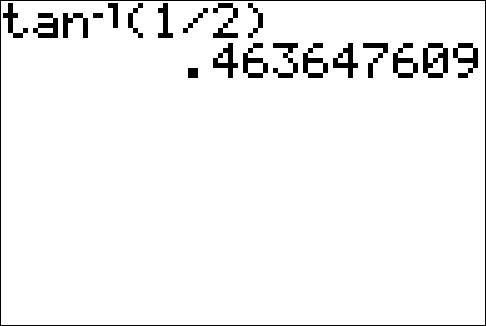
\includegraphics[width=2in]{./IntroTrigGraphics/ArcTrig01.jpg} &
\hspace{0.75in} 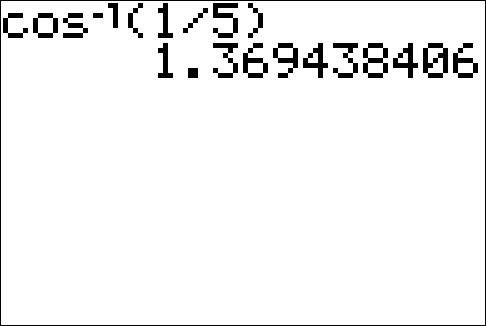
\includegraphics[width=2in]{./IntroTrigGraphics/ArcTrig02.jpg}  \\ 

\end{tabular} 

\item  Since the argument $-2$ is negative, we cannot directly apply  Theorem \ref{arctangentcotangentfunctionprops} to help us find  $\mbox{arccot}(-2)$.  Let $t = \mbox{arccot}(-2)$. Then $t$ is a real number such that $0 < t < \pi$ and $\cot(t) = -2$.  Moreover, since $\cot(t) < 0$, we know $\frac{\pi}{2} < t < \pi$.  Geometrically, this means $t$ corresponds to a Quadrant II angle $\theta = t$ radians.  This allows us to proceed using a `reference angle' approach. Consider $\alpha$, the reference angle for $\theta$, as pictured below. By definition, $\alpha$ is an acute angle so  $0 < \alpha < \frac{\pi}{2}$, and the Reference Angle Theorem, Theorem \ref{refanglethm}, tells us that $\cot(\alpha) = 2$.  This means  $\alpha = \mbox{arccot}(2)$ radians.  Since the argument of arccotangent is now a \emph{positive} $2$, we can use  Theorem \ref{arctangentcotangentfunctionprops} to get $\alpha = \mbox{arccot}(2) =\arctan\left(\frac{1}{2}\right)$ radians. Since $\theta = \pi - \alpha =  \pi - \arctan\left(\frac{1}{2}\right) \approx 2.6779$ radians, we get  $\mbox{arccot}(-2) \approx 2.6779$.

\begin{tabular}{m{2.5in}m{1in}m{2.5in}}


\begin{mfpic}[18]{-5}{5}{-5}{5}
\axes
\tlabel(5,-0.5){\scriptsize $x$}
\tlabel(0.25,5){\scriptsize $y$}
\tlabel(3.1,-0.75){\scriptsize $1$}
\tlabel(0.25,3.1){\scriptsize $1$}
\xmarks{-3 step 3 until 3}
\ymarks{-3 step 3 until 3}
\drawcolor[gray]{0.7}
\circle{(0,0),3}
\drawcolor[rgb]{0.33,0.33,0.33}
\arrow \polyline{(0,0), (-4.532, 2.113)}
\arrow \reverse \arrow \parafcn{157, 177, 5}{2.25*dir(t)}
\tlabel[cc](-2.75, 0.5){\scriptsize $\alpha$}
\point[3pt]{(0,0)}
\gclear \tlabelrect[cc](2.75, 2.5){\scriptsize \mbox{$\theta = \mbox{arccot}(-2)$ radians}}
\arrow \parafcn{0, 150, 5}{2.25*dir(t)}
\end{mfpic}


& 

&

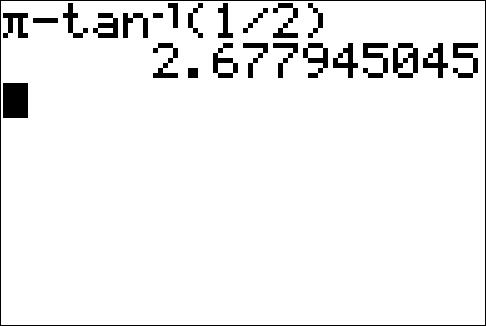
\includegraphics[width=2in]{./IntroTrigGraphics/ArcTrig03.jpg} \\

\end{tabular}

Another way to attack the problem is to use $\arctan\left(-\frac{1}{2}\right)$.  By definition, the real number $t = \arctan\left(-\frac{1}{2}\right)$ satisfies $\tan(t) = -\frac{1}{2}$ with $-\frac{\pi}{2} < t < \frac{\pi}{2}$.  Since $\tan(t)<0$, we know more specifically that $-\frac{\pi}{2} < t < 0$, so $t$ corresponds to an angle $\beta$ in Quadrant IV.  To find the value of $\mbox{arccot}(-2)$, we once again visualize the angle $\theta = \mbox{arccot}(-2)$ radians and note that it is a Quadrant II angle with $\tan(\theta) = -\frac{1}{2}$.  This means it is exactly $\pi$ units away from $\beta$, and we get $\theta = \pi + \beta = \pi + \arctan\left(-\frac{1}{2}\right) \approx 2.6779$ radians.  Hence, as before, $\mbox{arccot}(-2) \approx 2.6779$.

\begin{tabular}{m{2.5in}m{1in}m{2.5in}}

\begin{mfpic}[18]{-5}{5}{-5}{5}
\axes
\tlabel(5,-0.5){\scriptsize $x$}
\tlabel(0.25,5){\scriptsize $y$}
\tlabel(3.1,-0.75){\scriptsize $1$}
\tlabel(0.25,3.1){\scriptsize $1$}
\xmarks{-3 step 3 until 3}
\ymarks{-3 step 3 until 3}
\drawcolor[gray]{0.7}
\circle{(0,0),3}
\drawcolor[rgb]{0.33,0.33,0.33}
\arrow \polyline{(0,0), (-4.532, 2.113)}
\arrow \polyline{(0,0), (4.532, -2.113)}
\arrow \parafcn{-3, -23, -5}{2.25*dir(t)}
\arrow \reverse \arrow \parafcn{160,325,5}{2.25*dir(t)}
\tlabel[cc](-1.375,-2.382){\scriptsize $\pi$}
\tlabel[cc](2.5, -0.5){\scriptsize $\beta$}
\point[3pt]{(0,0)}
\gclear \tlabelrect[cc](2.75, 2.5){\mbox{\scriptsize $\theta = \mbox{arccot}(-2)$ radians}}
\arrow \parafcn{0, 150, 5}{2.25*dir(t)}
\end{mfpic}

& 

&

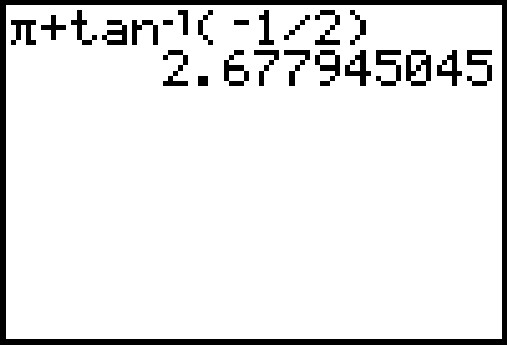
\includegraphics[width=2in]{./IntroTrigGraphics/ArcTrig03a.jpg} \\

\end{tabular}



\item If the range of arccosecant is taken to be $\left[-\frac{\pi}{2}, 0\right) \cup \left(0, \frac{\pi}{2}\right]$, we can use Theorem \ref{arcsecantcosecantfunctionprops1} to get $\mbox{arccsc}\left(-\frac{3}{2}\right) = \arcsin\left(-\frac{2}{3}\right) \approx -0.7297$.  If, on the other hand, the range of arccosecant is taken to be $\left(0, \frac{\pi}{2}\right] \cup \left(\pi, \frac{3\pi}{2}\right]$, then we proceed as in the previous problem by  letting $t = \mbox{arccsc}\left(-\frac{3}{2}\right)$.  Then $t$ is a real number with $\csc(t) = -\frac{3}{2}$.  Since $\csc(t) < 0$, we have that $\pi < \theta \leq \frac{3\pi}{2}$, so $t$ corresponds to a Quadrant III angle, $\theta$.  As above, we let $\alpha$ be the reference angle for $\theta$.  Then $0 < \alpha < \frac{\pi}{2}$ and $\csc(\alpha) =\frac{3}{2}$, which means $\alpha = \mbox{arccsc}\left(\frac{3}{2}\right)$ radians.  Since the argument of arccosecant is now positive, we may use Theorem \ref{arcsecantcosecantfunctionprops2}  to get $\alpha = \mbox{arccsc}\left(\frac{3}{2}\right) = \arcsin\left(\frac{2}{3}\right)$ radians.  Since $\theta = \pi + \alpha = \pi +  \arcsin\left(\frac{2}{3}\right) \approx 3.8713$ radians,  $\mbox{arccsc}\left(-\frac{3}{2}\right) \approx 3.8713$.

\begin{tabular}{m{2.5in}m{1in}m{2.5in}}

\begin{mfpic}[18]{-5}{5}{-5}{5}
\axes
\tlabel(5,-0.5){\scriptsize $x$}
\tlabel(0.25,5){\scriptsize $y$}
\tlabel(3.1,-0.75){\scriptsize $1$}
\tlabel(0.25,3.1){\scriptsize $1$}
\xmarks{-3 step 3 until 3}
\ymarks{-3 step 3 until 3}
\drawcolor[gray]{0.7}
\circle{(0,0),3}
\drawcolor[rgb]{0.33,0.33,0.33}
\arrow \polyline{(0,0), (-3.83, -3.21)}
\arrow \reverse \arrow \parafcn{185, 215, 5}{1.5*dir(t)}
\tlabel[cc](-1.88, -0.68){\scriptsize $\alpha$}
\point[3pt]{(0,0)}
\gclear \tlabelrect[cc](3.5, 2.5){\scriptsize $\theta = \mbox{arccsc}\left(-\frac{3}{2}\right)$ radians}
\arrow \parafcn{0, 215, 5}{2.5*dir(t)}
\end{mfpic}

& 

&

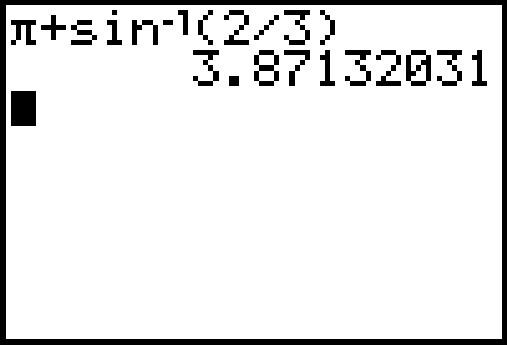
\includegraphics[width=2in]{./IntroTrigGraphics/ArcTrig04.jpg} \\

\end{tabular}

\end{enumerate}

\newpage

\item \begin{enumerate}

\item  Since the domain of $F(x) = \arccos(x)$ is $-1 \leq x \leq 1$, we can find the domain of $f(x) = \frac{\pi}{2} - \arccos\left(\frac{x}{5}\right)$ by setting the argument of the arccosine, in this case $\frac{x}{5}$, between $-1$ and $1$. Solving  $-1 \leq \frac{x}{5} \leq 1$ gives $-5 \leq x \leq 5$, so the domain is $[-5,5]$.  To determine the range of $f$, we take a cue from Section \ref{Transformations}. Three `key' points on the graph of $F(x) = \arccos(x)$ are  $(-1, \pi)$, $\left(0, \frac{\pi}{2}\right)$ and $(1,0)$ . Following the procedure outlined in Theorem \ref{transformationsthm}, we track these points to $\left(-5, -\frac{\pi}{2}\right)$, $(0, 0)$ and $\left(5, \frac{\pi}{2}\right)$. Plotting these values tells us that the range\footnote{It also confirms our domain!} of $f$ is $\left[-\frac{\pi}{2}, \frac{\pi}{2}\right]$. Our graph confirms our results.


\item  To find the domain and range of $f(x) = 3\arctan\left(4x \right)$, we note that since the domain of $F(x) = \arctan(x)$ is all real numbers, the only restrictions, if any, on the domain of  $f(x) = 3\arctan\left(4x \right)$ come from the argument of the arctangent, in this case, $4x$.  Since $4x$ is defined for all real numbers, we have established that the domain of $f$ is all real numbers.  To determine the range of $f$, we can, once again, appeal to Theorem \ref{transformationsthm}.  Choosing our `key' point to be $(0,0)$ and tracking the horizontal asymptotes $y = -\frac{\pi}{2}$ and $y= \frac{\pi}{2}$, we find that the graph of $y = f(x) = 3\arctan\left(4x \right)$ differs from the graph of $y = F(x) = \arctan(x)$ by a horizontal compression by a factor of $4$ and a vertical stretch by a factor of $3$.  It is the latter which affects the range, producing a range of $\left(-\frac{3\pi}{2}, \frac{3\pi}{2} \right)$.  We confirm our findings on the calculator below.

\smallskip

\begin{tabular}{cc}

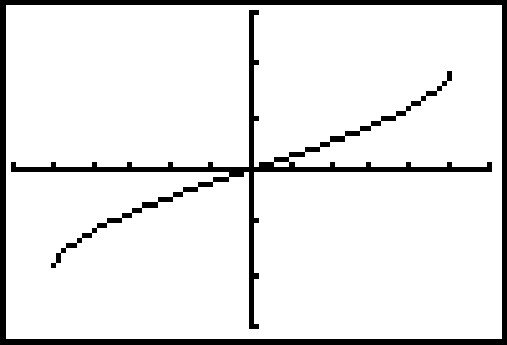
\includegraphics[width=2in]{./IntroTrigGraphics/ARCCOS01.jpg} &
\hspace{0.75in} 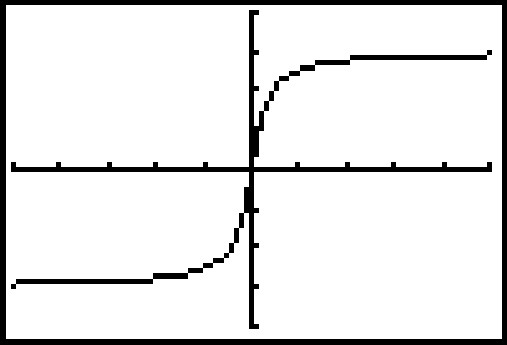
\includegraphics[width=2in]{./IntroTrigGraphics/ARCTAN01.jpg}  \\

$y =f(x) = \dfrac{\pi}{2} - \arccos\left(\dfrac{x}{5}\right)$ & \hspace{0.75in} $y = f(x) = 3\arctan\left(4x \right)$
\end{tabular} 

\item  To find the domain of $g(x) = \text{arccot}\left(\frac{x}{2}\right) + \pi$, we proceed as above.  Since the domain of $G(x) = \text{arccot}(x)$ is $(-\infty, \infty)$, and $\frac{x}{2}$ is defined for all $x$, we get that the domain of $g$ is $(-\infty, \infty)$ as well.  As for the range, we note that the range of $G(x)  = \text{arccot}(x)$, like that of $F(x) = \arctan(x)$, is limited by a pair of horizontal asymptotes, in this case $y = 0$ and $y = \pi$.  Following  Theorem \ref{transformationsthm}, we graph $y =  g(x) = \text{arccot}\left(\frac{x}{2}\right) + \pi$ starting with $y = G(x) = \text{arccot}(x)$ and first performing a horizontal expansion by a factor of $2$ and following that with a vertical shift upwards by $\pi$.  This latter transformation is the one which affects the range, making it now $(\pi, 2\pi)$.  To check this graphically, we encounter a bit of a problem, since on many calculators, there is no shortcut button corresponding to the arccotangent function. Taking a cue from number \ref{arccotneg2}, we attempt to rewrite $g(x) = \text{arccot}\left(\frac{x}{2}\right) + \pi$ in terms of the arctangent function. Using Theorem \ref{arctangentcotangentfunctionprops}, we have that $\text{arccot}\left(\frac{x}{2}\right) = \arctan\left(\frac{2}{x}\right)$ when $\frac{x}{2} > 0$, or, in this case, when $x > 0$.  Hence, for $x > 0$, we have $g(x) = \arctan\left(\frac{2}{x}\right) + \pi$.  When $\frac{x}{2} < 0$, we can use the same argument in number \ref{arccotneg2} that gave us $\text{arccot}(-2) = \pi + \arctan\left(-\frac{1}{2}\right)$ to give us $\text{arccot}\left(\frac{x}{2}\right) = \pi + \arctan\left(\frac{2}{x}\right)$.  Hence, for $x < 0$, $g(x) = \pi + \arctan\left(\frac{2}{x}\right) + \pi = \arctan\left(\frac{2}{x}\right) + 2\pi$.  What about $x=0$?  We know $g(0) = \text{arccot}(0) + \pi = \pi$, and neither of the formulas for $g$ involving arctangent will produce this result.\footnote{Without Calculus, of course \ldots}  Hence, in order to graph $y = g(x)$ on our calculators, we need to write it as a piecewise defined function:

\[ g(x) = \text{arccot}\left(\frac{x}{2}\right) + \pi = \left\{ \begin{array}{rr} \arctan\left(\frac{2}{x}\right) + 2\pi, & \text{if $x<0$} \\ [5pt] \pi, & \text{if $x=0$} \\ [5pt] \arctan\left(\frac{2}{x}\right) + \pi, & \text{if $x>0$} \end{array}\right. \]

We show the input and the result below.

\smallskip

\begin{tabular}{cc}

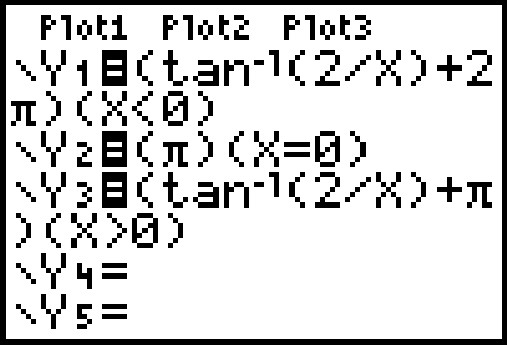
\includegraphics[width=2in]{./IntroTrigGraphics/ARCCOT01.jpg} &
\hspace{0.75in} 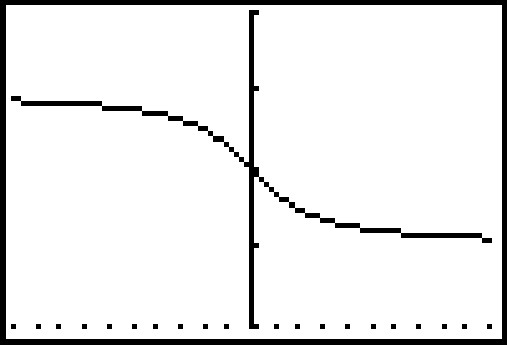
\includegraphics[width=2in]{./IntroTrigGraphics/ARCCOT02.jpg}  \\

$y=g(x)$ in terms of arctangent & \hspace{0.75in} $y = g(x) = \text{arccot}\left(\frac{x}{2}\right) + \pi $
\end{tabular} 

\end{enumerate}

\end{enumerate}

\qed
\end{ex}





The inverse trigonometric functions are typically found in applications whenever the measure of an angle is required.  One such scenario is presented in the following example.


\begin{ex}\footnote{The authors would like to thank Dan Stitz for this problem and associated graphics.} \label{roofpitchex}  The roof on the house below has a  `$6/12$ pitch'.  This means that when viewed from the side, the roof line has a rise of 6 feet over a run of 12 feet.  Find the angle of inclination from the bottom of the roof to the top of the roof.  Express your answer in decimal degrees, rounded to the nearest hundredth of a degree.

\begin{center}

\begin{tabular}{cc}

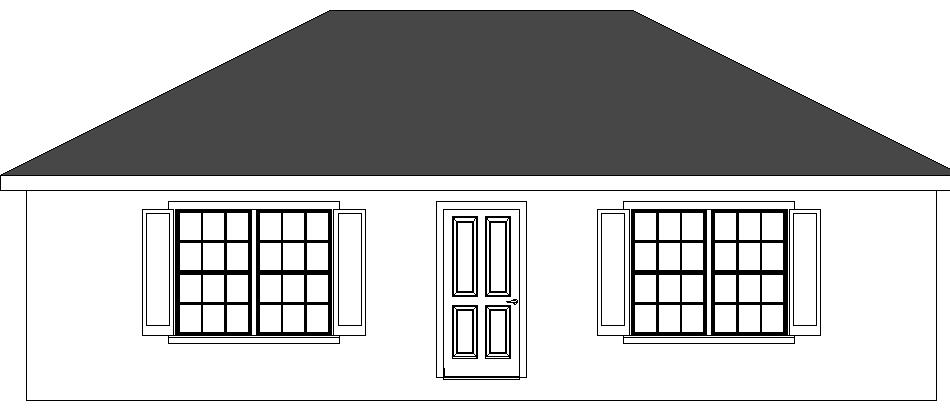
\includegraphics[width=2.75in]{./IntroTrigGraphics/ArcTrig05.jpg} &
\hspace{0.75in} 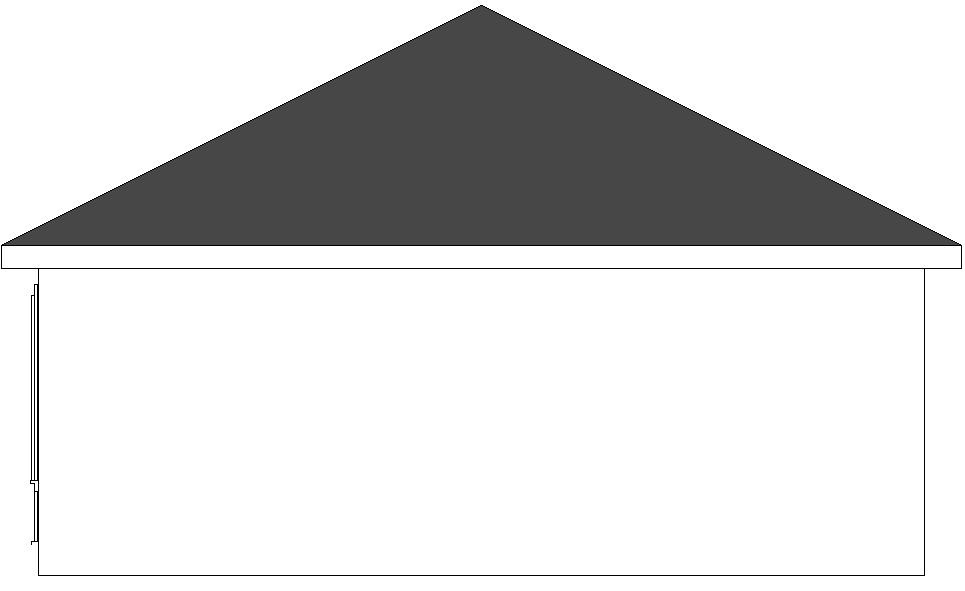
\includegraphics[width=2in]{./IntroTrigGraphics/ArcTrig06.jpg}  \\ 
Front View &  \hspace{0.75in} Side View \\

\end{tabular} 

\end{center}

{\bf Solution.} If we divide the side view of the house down the middle, we find that the roof line forms the hypotenuse of a right triangle with legs of length $6$ feet and $12$ feet.  Using Theorem \ref{circularfunctionstriangle}, we find the angle of inclination, labeled $\theta$ below, satisfies $\tan(\theta) = \frac{6}{12} = \frac{1}{2}$.  Since $\theta$ is an acute angle, we can use the arctangent function and we find $\theta = \arctan\left(\frac{1}{2}\right)\, \text{radians} \, \approx 26.56^{\circ}$.



\begin{tabular}{m{2.5in}m{1in}m{2.5in}}

\begin{mfpic}[15]{0}{13.25}{-1}{6}

\polyline{(0,0), (12,0), (12,6), (0,0)}
\polyline{(11.25,0), (11.25,0.75), (12,0.75)}
\arrow \reverse \arrow \polyline{(0,-1),(12,-1)}
\gclear \tlabelrect[cc](6,-1){$12$ feet}
\arrow \reverse \arrow \polyline{(13.25,0),(13.25,6)}
\gclear \tlabelrect[cc](13.25,3){$6$ feet}
\arrow \parafcn{3, 19, 5}{2.75*dir(t)}
\tlabel[cc](3.25,0.5){$\theta$}
\end{mfpic}

& 

&

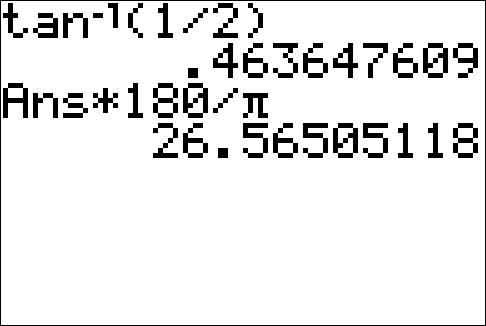
\includegraphics[width=2in]{./IntroTrigGraphics/ArcTrig07.jpg} \qed \\

\end{tabular}

\end{ex}

\subsection{Solving Equations Using the Inverse Trigonometric Functions.}

In Sections \ref{TheUnitCircle} and \ref{CircularFunctions}, we learned how to solve equations like $\sin(\theta) = \frac{1}{2}$ for angles $\theta$ and $\tan(t) = -1$ for real numbers $t$. In each case, we ultimately appealed to the Unit Circle and relied on the fact that the answers corresponded to a set of `common angles' listed on page \pageref{commonanglesunitcircle}.  If, on the other hand, we had been asked to find all angles with $\sin(\theta) = \frac{1}{3}$ or solve $\tan(t) = -2$ for real numbers $t$, we would have been hard-pressed to do so.  With the introduction of the inverse trigonometric functions, however, we are now in a position to solve these equations. A good parallel to keep in mind is how the square root function can be used to solve certain quadratic equations.  The equation $x^2 = 4$ is a lot like  $\sin(\theta) = \frac{1}{2}$ in that it has friendly, `common value' answers  $x = \pm 2$.  The equation $x^2 = 7$, on the other hand, is a lot like $\sin(\theta) = \frac{1}{3}$.  We know\footnote{How do we know this again?} there are answers, but we can't express them using `friendly' numbers.\footnote{This is all, of course, a matter of opinion.  For the record, the authors find $\pm \sqrt{7}$ just as `nice' as $\pm 2$.}  To solve $x^2 = 7$, we make use of the square root function and write $x = \pm \sqrt{7}$. We can certainly \textit{approximate} these answers using a calculator, but as far as exact answers go, we leave them as $x = \pm \sqrt{7}$.  In the same way, we will use the arcsine function to solve $\sin(\theta) = \frac{1}{3}$, as seen in the following example.

\begin{ex}  \label{basicinverseeqns}  Solve the following equations.

\begin{enumerate}

\item  \label{basicinverseeqnssine} Find all angles $\theta$ for which $\sin(\theta) = \frac{1}{3}$.

\item \label{basicinverseeqnstangent} Find all real numbers $t$ for which $\tan(t) = -2$

\item  \label{basicinverseeqnssecant} Solve $\, \sec(x) = -\frac{5}{3} \,$ for $x$.

\end{enumerate}

{\bf Solution.}  

\begin{enumerate}

\item  If $\sin(\theta) = \frac{1}{3}$, then the terminal side of $\theta$, when plotted in standard position, intersects the Unit Circle at $y = \frac{1}{3}$.  Geometrically, we see that this happens at two places:  in Quadrant I and Quadrant II. If we let $\alpha$ denote the acute solution to the equation, then all the solutions to this equation in Quadrant I  are coterminal with $\alpha$, and $\alpha$ serves as the reference angle for all of the solutions to this equation in Quadrant II.

\begin{tabular}{cc}

\begin{mfpic}[18]{-5}{5}{-5}{5}
\axes
\tlabel(5,-0.5){\scriptsize $x$}
\tlabel(0.25,5){\scriptsize $y$}
\tlabel(3.1,-0.75){\scriptsize $1$}
\tlabel(0.25,3.1){\scriptsize $1$}
\xmarks{-3 step 3 until 3}
\ymarks{-3, 1, 3}
\tlpointsep{4pt}
\axislabels{y}{{\scriptsize $\frac{1}{3}$} 1}
\drawcolor[gray]{0.7}
\circle{(0,0),3}
\drawcolor[rgb]{0.33,0.33,0.33}
\arrow \polyline{(0,0), (4.532, 2.113)}
\arrow \parafcn{5, 20, 5}{2.75*dir(t)}
\tlabel[cc](5.5, 0.61){\scriptsize $\alpha = \arcsin\left(\frac{1}{3}\right)$ radians}
\end{mfpic}

&

\hspace{0.25in}

\begin{mfpic}[18]{-5}{5}{-5}{5}
\axes
\tlabel(5,-0.5){\scriptsize $x$}
\tlabel(0.25,5){\scriptsize $y$}
\tlabel(3.1,-0.75){\scriptsize $1$}
\tlabel(0.25,3.1){\scriptsize $1$}
\xmarks{-3 step 3 until 3}
\ymarks{-3, 1, 3}
\tlpointsep{4pt}
\axislabels{y}{{\scriptsize $\frac{1}{3}$} 1}
\drawcolor[gray]{0.7}
\circle{(0,0),3}
\drawcolor[rgb]{0.33,0.33,0.33}
\arrow \polyline{(0,0), (-4.532, 2.113)}
\arrow \reverse \arrow \parafcn{160, 175, 5}{2.75*dir(t)}
\tlabel[cc](-3.45, 0.61){\scriptsize $\alpha$}
\end{mfpic} \\

\end{tabular}

Since $\frac{1}{3}$ isn't the sine of any of the `common angles' discussed earlier, we use the arcsine functions to express our answers.  The real number $t = \arcsin\left(\frac{1}{3}\right)$ is defined so it satisfies $0 < t < \frac{\pi}{2}$ with $\sin(t) = \frac{1}{3}$.  Hence, $\alpha = \arcsin\left(\frac{1}{3}\right)$ radians. Since the solutions in Quadrant I are all coterminal with $\alpha$, we get part of our solution to be $\theta = \alpha + 2\pi k  = \arcsin\left(\frac{1}{3}\right) + 2\pi k$ for integers $k$.  Turning our attention to Quadrant II, we get one solution to be $\pi - \alpha$.  Hence, the Quadrant II solutions are  $\theta = \pi - \alpha + 2\pi k = \pi - \arcsin\left(\frac{1}{3}\right) + 2\pi k$, for integers $k$.


\item We may visualize the solutions to $\tan(t)=-2$ as angles $\theta$  with $\tan(\theta) = -2$.  Since tangent is negative only in Quadrants II and IV, we focus our efforts there. 


\begin{tabular}{cc}

\begin{mfpic}[18]{-5}{5}{-5}{5}
\axes
\tlabel(5,-0.5){\scriptsize $x$}
\tlabel(0.25,5){\scriptsize $y$}
\tlabel(3.1,0.75){\scriptsize $1$}
\tlabel(0.25,3.1){\scriptsize $1$}
\xmarks{-3 step 3 until 3}
\ymarks{-3 step 3 until 3}
\drawcolor[gray]{0.7}
\circle{(0,0),3}
\drawcolor[rgb]{0.33,0.33,0.33}
\arrow \polyline{(0,0), (2.5, -4.3301)}
\arrow \parafcn{355, 305, -5}{1.5*dir(t)}
\gclear \tlabelrect[cc](4, -1){\scriptsize $\beta = \arctan(-2)$ radians}
\end{mfpic}

&

\hspace{.25in}


\begin{mfpic}[18]{-5}{5}{-5}{5}
\axes
\tlabel(5,-0.5){\scriptsize $x$}
\tlabel(0.25,5){\scriptsize $y$}
\tlabel(3.1,0.75){\scriptsize $1$}
\tlabel(0.25,3.1){\scriptsize $1$}
\xmarks{-3 step 3 until 3}
\ymarks{-3 step 3 until 3}
\drawcolor[gray]{0.7}
\circle{(0,0),3}
\drawcolor[rgb]{0.33,0.33,0.33}
\arrow \polyline{(0,0), (-2.5, 4.3301)}
\arrow \polyline{(0,0), (2.5, -4.3301)}
\arrow \parafcn{355, 305, -5}{1.5*dir(t)}
\arrow \reverse \arrow \parafcn{125, 295, 5}{1.5*dir(t)}
\tlabel[cc](-2, -1){\scriptsize $\pi$}
\tlabel[cc](2, -1){\scriptsize $\beta$}

\end{mfpic} \\

\end{tabular}

Since $-2$ isn't the tangent of any of the `common angles', we need to use the arctangent function to express our answers.  The real number $t = \arctan(-2)$ satisfies $\tan(t)=-2$  and $-\frac{\pi}{2} < t < 0$.   If we let $\beta = \arctan(-2)$ radians, we see that all of the Quadrant IV solutions to  $\tan(\theta) = -2$  are coterminal with $\beta$. Moreover, the solutions from Quadrant II differ by exactly $\pi$ units from the solutions in Quadrant IV, so all the solutions to $\tan(\theta) = -2$ are of the form $\theta = \beta + \pi k = \arctan(-2) + \pi k$ for some integer $k$.  Switching back to the variable $t$,  we record our final answer to $\tan(t) = -2$ as $t = \arctan(-2) + \pi k$ for integers $k$.


\item  The last equation we are asked to solve, $\sec(x) = -\frac{5}{3}$, poses two immediate problems.  First, we are not told whether or not $x$ represents an angle or a real number.  We assume the latter, but note that we will use angles and the Unit Circle to solve the equation regardless.  Second, as we have mentioned, there is no universally accepted range of the arcsecant function.  For that reason, we adopt the advice given in Section \ref{CircularFunctions} and convert this to the cosine problem $\cos(x) = -\frac{3}{5}$.  Adopting an angle approach, we consider the equation $\cos(\theta) = -\frac{3}{5}$ and note that our solutions lie in Quadrants II and III.  Since $-\frac{3}{5}$ isn't  the cosine of any of the `common angles', we'll need to express our solutions in terms of the arccosine function.  The real number $t = \arccos\left(-\frac{3}{5}\right)$ is defined so that $\frac{\pi}{2} < t < \pi$ with $\cos(t) = -\frac{3}{5}$.  If we let $\beta = \arccos\left(-\frac{3}{5}\right)$ radians, we see that $\beta$ is a Quadrant II angle.  To obtain a Quadrant III angle solution, we may simply use $-\beta = -\arccos\left(-\frac{3}{5}\right)$.  Since all angle solutions are coterminal with $\beta$ or $-\beta$, we get our solutions to $\cos(\theta) = -\frac{3}{5}$ to be $\theta = \beta + 2\pi k = \arccos\left(-\frac{3}{5}\right) + 2\pi k$ or $\theta = -\beta + 2\pi k = -\arccos\left(-\frac{3}{5}\right) + 2\pi k$ for integers $k$.  Switching back to the variable $x$,  we record our final answer to $\sec(x) = -\frac{5}{3}$ as $x = \arccos\left(-\frac{3}{5}\right) + 2\pi k$ or $x = -\arccos\left(-\frac{3}{5}\right) + 2\pi k$ for integers $k$.

\begin{tabular}{cc}


\begin{mfpic}[18]{-5}{5}{-5}{5}
\axes
\tlabel(5,-0.5){\scriptsize $x$}
\tlabel(0.25,5){\scriptsize $y$}
\tlabel(3.1,-0.75){\scriptsize $1$}
\tlabel(0.25,3.1){\scriptsize $1$}
\xmarks{-3 step 3 until 3}
\ymarks{-3 step 3 until 3}
\drawcolor[gray]{0.7}
\circle{(0,0),3}
\drawcolor[rgb]{0.33,0.33,0.33}
\arrow \polyline{(0,0), (-2.5, 4.3301)}
\arrow \parafcn{5, 115, 5}{1.5*dir(t)}
\gclear \tlabelrect[cc](4, 1.5){\scriptsize $\beta = \arccos\left(-\frac{3}{5}\right)$ radians}
\end{mfpic}
&

\hspace{-.15in}

\begin{mfpic}[18]{-5}{5}{-5}{5}
\axes
\tlabel(5,-0.5){\scriptsize $x$}
\tlabel(0.25,5){\scriptsize $y$}
\tlabel(3.1,-0.75){\scriptsize $1$}
\tlabel(0.25,3.1){\scriptsize $1$}
\xmarks{-3 step 3 until 3}
\ymarks{-3 step 3 until 3}
\drawcolor[gray]{0.7}
\circle{(0,0),3}
\drawcolor[rgb]{0.33,0.33,0.33}
\dashed \polyline{(0,0), (-2.5, 4.3301)}
\arrow \dotted \parafcn{5, 115, 5}{1.5*dir(t)}
\gclear \tlabelrect[cc](4, 1.5){\scriptsize $\beta = \arccos\left(-\frac{3}{5}\right)$ radians}
\arrow \polyline{(0,0), (-2.5, -4.3301)}
\arrow \parafcn{355, 245, -5}{1.5*dir(t)}
\gclear \tlabelrect[cc](4, -1.5){\scriptsize $-\beta = -\arccos\left(-\frac{3}{5}\right)$ radians}
\end{mfpic} \qed \\


\end{tabular}

\end{enumerate}

\end{ex}

 The reader is encouraged to check the answers found in Example \ref{basicinverseeqns} - both analytically and with the calculator (see Section \ref{sectionarcstuffoncalc}).  With practice, the inverse trigonometric functions will become as familiar to you as the square root function.  Speaking of practice \dots


\newpage

\subsection{Exercises}

In Exercises \ref{exactvaluearcfirst} - \ref{exactvaluearclast}, find the exact value.

\begin{multicols}{4} 

\begin{enumerate}

\item $\arcsin \left( -1 \right)$ \vphantom{$\left( -\dfrac{\sqrt{3}}{2} \right)$} \label{exactvaluearcfirst}
\item $\arcsin \left( -\dfrac{\sqrt{3}}{2} \right)$
\item $\arcsin \left( -\dfrac{\sqrt{2}}{2} \right)$
\item $\arcsin \left( -\dfrac{1}{2} \right)$ \vphantom{$\left( -\dfrac{\sqrt{3}}{2} \right)$}

\setcounter{HW}{\value{enumi}}

\end{enumerate}

\end{multicols}

\begin{multicols}{4}

\begin{enumerate}

\setcounter{enumi}{\value{HW}}

\item $\arcsin \left( 0 \right)$ \vphantom{$\left( \dfrac{\sqrt{3}}{2} \right)$}
\item $\arcsin \left( \dfrac{1}{2} \right)$ \vphantom{$\left( \dfrac{\sqrt{3}}{2} \right)$}
\item $\arcsin \left( \dfrac{\sqrt{2}}{2} \right)$
\item $\arcsin \left( \dfrac{\sqrt{3}}{2} \right)$

\setcounter{HW}{\value{enumi}}

\end{enumerate}

\end{multicols}

\begin{multicols}{4}

\begin{enumerate}

\setcounter{enumi}{\value{HW}}

\item $\arcsin \left( 1 \right)$ \vphantom{$\left( -\dfrac{\sqrt{3}}{2} \right)$}
\item $\arccos \left( -1 \right)$ \vphantom{$\left( -\dfrac{\sqrt{3}}{2} \right)$}
\item $\arccos \left( -\dfrac{\sqrt{3}}{2} \right)$
\item $\arccos \left( -\dfrac{\sqrt{2}}{2} \right)$

\setcounter{HW}{\value{enumi}}

\end{enumerate}

\end{multicols}

\begin{multicols}{4}

\begin{enumerate}

\setcounter{enumi}{\value{HW}}

\item $\arccos \left( -\dfrac{1}{2} \right)$ \vphantom{$\left( \dfrac{\sqrt{3}}{2} \right)$}
\item $\arccos \left( 0 \right)$ \vphantom{$\left( \dfrac{\sqrt{3}}{2} \right)$}
\item $\arccos \left( \dfrac{1}{2} \right)$ \vphantom{$\left( \dfrac{\sqrt{3}}{2} \right)$}
\item $\arccos \left( \dfrac{\sqrt{2}}{2} \right)$

\setcounter{HW}{\value{enumi}}

\end{enumerate}

\end{multicols}

\begin{multicols}{4}

\begin{enumerate}

\setcounter{enumi}{\value{HW}}

\item $\arccos \left( \dfrac{\sqrt{3}}{2} \right)$
\item $\arccos \left( 1 \right)$ \vphantom{$\left( \dfrac{\sqrt{3}}{2} \right)$}
\item $\arctan \left( -\sqrt{3} \right)$ \vphantom{$\left( \dfrac{\sqrt{3}}{2} \right)$}
\item $\arctan \left( -1 \right)$ \vphantom{$\left( \dfrac{\sqrt{3}}{2} \right)$}

\setcounter{HW}{\value{enumi}}

\end{enumerate}

\end{multicols}

\begin{multicols}{4}

\begin{enumerate}

\setcounter{enumi}{\value{HW}}

\item $\arctan \left( -\dfrac{\sqrt{3}}{3} \right)$
\item $\arctan \left( 0 \right)$ \vphantom{$\left( -\dfrac{\sqrt{3}}{2} \right)$}
\item $\arctan \left( \dfrac{\sqrt{3}}{3} \right)$
\item $\arctan \left( 1 \right)$ \vphantom{$\left( -\dfrac{\sqrt{3}}{2} \right)$}

\setcounter{HW}{\value{enumi}}

\end{enumerate}

\end{multicols}

\begin{multicols}{4}

\begin{enumerate}

\setcounter{enumi}{\value{HW}}

\item $\arctan \left( \sqrt{3} \right)$ \vphantom{$\left( -\dfrac{\sqrt{3}}{2} \right)$}
\item $\mbox{arccot} \left( -\sqrt{3} \right)$ \vphantom{$\left( -\dfrac{\sqrt{3}}{2} \right)$}
\item $\mbox{arccot} \left( -1 \right)$ \vphantom{$\left( -\dfrac{\sqrt{3}}{2} \right)$}
\item $\mbox{arccot} \left( -\dfrac{\sqrt{3}}{3} \right)$

\setcounter{HW}{\value{enumi}}

\end{enumerate}

\end{multicols}

\begin{multicols}{4}

\begin{enumerate}

\setcounter{enumi}{\value{HW}}

\item $\mbox{arccot} \left( 0 \right)$ \vphantom{$\left( -\dfrac{\sqrt{3}}{2} \right)$}
\item $\mbox{arccot} \left( \dfrac{\sqrt{3}}{3} \right)$
\item $\mbox{arccot} \left( 1 \right)$ \vphantom{$\left( -\dfrac{\sqrt{3}}{2} \right)$}
\item $\mbox{arccot} \left( \sqrt{3} \right)$ \vphantom{$\left( -\dfrac{\sqrt{3}}{2} \right)$}

\setcounter{HW}{\value{enumi}}

\end{enumerate}

\end{multicols}

\begin{multicols}{4}

\begin{enumerate}

\setcounter{enumi}{\value{HW}}

\item $\mbox{arcsec} \left( 2 \right)$
\item $\mbox{arccsc} \left( 2 \right)$
\item $\mbox{arcsec} \left( \sqrt{2} \right)$
\item $\mbox{arccsc} \left( \sqrt{2} \right)$

\setcounter{HW}{\value{enumi}}

\end{enumerate}

\end{multicols}

\begin{multicols}{4}

\begin{enumerate}

\setcounter{enumi}{\value{HW}}

\item $\mbox{arcsec} \left( \dfrac{2\sqrt{3}}{3} \right)$
\item $\mbox{arccsc} \left( \dfrac{2\sqrt{3}}{3} \right)$
\item $\mbox{arcsec} \left( 1 \right)$ \vphantom{$\left( -\dfrac{\sqrt{3}}{2} \right)$}
\item $\mbox{arccsc} \left( 1 \right)$ \vphantom{$\left( -\dfrac{\sqrt{3}}{2} \right)$} \label{exactvaluearclast}

\setcounter{HW}{\value{enumi}}

\end{enumerate}

\end{multicols}

In Exercises \ref{calcfriendexactfirst} - \ref{calcfriendexactlast}, assume that the range of arcsecant is $\left[0, \frac{\pi}{2} \right) \cup \left[\pi, \frac{3\pi}{2} \right)$ and that the range of arccosecant is $\left(0, \frac{\pi}{2} \right] \cup \left( \pi, \frac{3\pi}{2} \right]$ when finding the exact value.

\begin{multicols}{4} 

\begin{enumerate}

\setcounter{enumi}{\value{HW}}

\item $\mbox{arcsec} \left( -2 \right)$ \vphantom{$\left( -\dfrac{2\sqrt{3}}{3} \right)$} \label{calcfriendexactfirst}
\item $\mbox{arcsec} \left( -\sqrt{2} \right)$ \vphantom{$\left( -\dfrac{2\sqrt{3}}{3} \right)$} 
\item $\mbox{arcsec} \left( -\dfrac{2\sqrt{3}}{3} \right)$
\item $\mbox{arcsec} \left( -1 \right)$ \vphantom{$\left( -\dfrac{2\sqrt{3}}{3} \right)$} 

\setcounter{HW}{\value{enumi}}

\end{enumerate}

\end{multicols}

\begin{multicols}{4}

\begin{enumerate}

\setcounter{enumi}{\value{HW}}

\item $\mbox{arccsc} \left( -2 \right)$ \vphantom{$\left( -\dfrac{2\sqrt{3}}{3} \right)$} 
\item $\mbox{arccsc} \left( -\sqrt{2} \right)$ \vphantom{$\left( -\dfrac{2\sqrt{3}}{3} \right)$} 
\item $\mbox{arccsc} \left( -\dfrac{2\sqrt{3}}{3} \right)$ 
\item $\mbox{arccsc} \left( -1 \right)$ \vphantom{$\left( -\dfrac{2\sqrt{3}}{3} \right)$}  \label{calcfriendexactlast}

\setcounter{HW}{\value{enumi}}

\end{enumerate}

\end{multicols}

\pagebreak

In Exercises \ref{trigfriendexactfirst} - \ref{trigfriendexactlast}, assume that the range of arcsecant is $\left[0, \frac{\pi}{2} \right) \cup \left( \frac{\pi}{2}, \pi \right]$ and that the range of arccosecant is
$\left[ -\frac{\pi}{2}, 0 \right)  \cup \left(0, \frac{\pi}{2} \right]$ when finding the exact value.

\begin{multicols}{4} 

\begin{enumerate}

\setcounter{enumi}{\value{HW}}

\item $\mbox{arcsec} \left( -2 \right)$ \vphantom{$\left( -\dfrac{2\sqrt{3}}{3} \right)$} \label{trigfriendexactfirst}
\item $\mbox{arcsec} \left( -\sqrt{2} \right)$ \vphantom{$\left( -\dfrac{2\sqrt{3}}{3} \right)$} 
\item $\mbox{arcsec} \left( -\dfrac{2\sqrt{3}}{3} \right)$
\item $\mbox{arcsec} \left( -1 \right)$ \vphantom{$\left( -\dfrac{2\sqrt{3}}{3} \right)$} 

\setcounter{HW}{\value{enumi}}

\end{enumerate}

\end{multicols}

\begin{multicols}{4}

\begin{enumerate}

\setcounter{enumi}{\value{HW}}

\item $\mbox{arccsc} \left( -2 \right)$ \vphantom{$\left( -\dfrac{2\sqrt{3}}{3} \right)$} 
\item $\mbox{arccsc} \left( -\sqrt{2} \right)$ \vphantom{$\left( -\dfrac{2\sqrt{3}}{3} \right)$} 
\item $\mbox{arccsc} \left( -\dfrac{2\sqrt{3}}{3} \right)$
\item $\mbox{arccsc} \left( -1 \right)$ \vphantom{$\left( -\dfrac{2\sqrt{3}}{3} \right)$}  \label{trigfriendexactlast}

\setcounter{HW}{\value{enumi}}

\end{enumerate}

\end{multicols}

In Exercises \ref{comboexactfirst} - \ref{comboexactlast}, find the exact value or state that it is undefined.

\begin{multicols}{3} 

\begin{enumerate}

\setcounter{enumi}{\value{HW}}

\item $\sin\left(\arcsin\left(\dfrac{1}{2}\right)\right)$ \vphantom{$\left( -\dfrac{\sqrt{2}}{2} \right)$} \label{comboexactfirst}
\item $\sin\left(\arcsin\left(-\dfrac{\sqrt{2}}{2}\right)\right)$
\item $\sin\left(\arcsin\left(\dfrac{3}{5}\right)\right)$ \vphantom{$\left( -\dfrac{\sqrt{2}}{2} \right)$}

\setcounter{HW}{\value{enumi}}

\end{enumerate}

\end{multicols}

\begin{multicols}{3}

\begin{enumerate}

\setcounter{enumi}{\value{HW}}

\item $\sin\left(\arcsin\left(-0.42\right)\right)$ \vphantom{$\left( \dfrac{\sqrt{2}}{2} \right)$}
\item $\sin\left(\arcsin\left(\dfrac{5}{4}\right)\right)$ \vphantom{$\left( \dfrac{\sqrt{2}}{2} \right)$}
\item $\cos\left(\arccos\left(\dfrac{\sqrt{2}}{2}\right)\right)$

\setcounter{HW}{\value{enumi}}

\end{enumerate}

\end{multicols}

\begin{multicols}{3}

\begin{enumerate}

\setcounter{enumi}{\value{HW}}

\item $\cos\left(\arccos\left(-\dfrac{1}{2}\right)\right)$
\item $\cos\left(\arccos\left(\dfrac{5}{13}\right)\right)$
\item $\cos\left(\arccos\left(-0.998\right)\right)$ \vphantom{$\left( -\dfrac{1}{2} \right)$}

\setcounter{HW}{\value{enumi}}

\end{enumerate}

\end{multicols}

\begin{multicols}{3}

\begin{enumerate}

\setcounter{enumi}{\value{HW}}

\item $\cos\left(\arccos\left(\pi \right)\right)$
\item $\tan\left(\arctan\left(-1\right)\right)$
\item $\tan\left(\arctan\left(\sqrt{3}\right)\right)$

\setcounter{HW}{\value{enumi}}

\end{enumerate}

\end{multicols}

\begin{multicols}{3}

\begin{enumerate}

\setcounter{enumi}{\value{HW}}

\item $\tan\left(\arctan\left(\dfrac{5}{12}\right)\right)$
\item $\tan\left(\arctan\left(0.965\right)\right)$ \vphantom{$\left( \dfrac{1}{2} \right)$}
\item $\tan\left(\arctan\left( 3\pi \right)\right)$ \vphantom{$\left( \dfrac{1}{2} \right)$}

\setcounter{HW}{\value{enumi}}

\end{enumerate}

\end{multicols}

\begin{multicols}{3}

\begin{enumerate}

\setcounter{enumi}{\value{HW}}

\item $\cot\left(\text{arccot}\left(1\right)\right)$ \vphantom{$\left( \dfrac{1}{2} \right)$}
\item $\cot\left(\text{arccot}\left(-\sqrt{3}\right)\right)$ \vphantom{$\left( \dfrac{1}{2} \right)$}
\item $\cot\left(\text{arccot}\left(-\dfrac{7}{24}\right)\right)$

\setcounter{HW}{\value{enumi}}

\end{enumerate}

\end{multicols}

\begin{multicols}{3}

\begin{enumerate}

\setcounter{enumi}{\value{HW}}

\item $\cot\left(\text{arccot}\left(-0.001\right)\right)$ \vphantom{$\left( \dfrac{1}{2} \right)$}
\item $\cot\left(\text{arccot}\left( \dfrac{17\pi}{4} \right)\right)$
\item $\sec\left(\text{arcsec}\left(2\right)\right)$ \vphantom{$\left( \dfrac{1}{2} \right)$}

\setcounter{HW}{\value{enumi}}

\end{enumerate}

\end{multicols}

\begin{multicols}{3}

\begin{enumerate}

\setcounter{enumi}{\value{HW}}

\item $\sec\left(\text{arcsec}\left(-1\right)\right)$ \vphantom{$\left( \dfrac{1}{2} \right)$}
\item $\sec\left(\text{arcsec}\left(\dfrac{1}{2}\right)\right)$
\item $\sec\left(\text{arcsec}\left(0.75\right)\right)$ \vphantom{$\left( \dfrac{1}{2} \right)$}

\setcounter{HW}{\value{enumi}}

\end{enumerate}

\end{multicols}

\begin{multicols}{3}

\begin{enumerate}

\setcounter{enumi}{\value{HW}}

\item $\sec\left(\text{arcsec}\left( 117\pi \right)\right)$ \vphantom{$\left( \dfrac{\sqrt{3}}{3} \right)$}
\item $\csc\left(\text{arccsc}\left(\sqrt{2}\right)\right)$ \vphantom{$\left( \dfrac{\sqrt{3}}{3} \right)$}
\item $\csc\left(\text{arccsc}\left(-\dfrac{2\sqrt{3}}{3}\right)\right)$

\setcounter{HW}{\value{enumi}}

\end{enumerate}

\end{multicols}

\begin{multicols}{3}

\begin{enumerate}

\setcounter{enumi}{\value{HW}}

\item $\csc\left(\text{arccsc}\left(\dfrac{\sqrt{2}}{2}\right)\right)$
\item $\csc\left(\text{arccsc}\left(1.0001\right)\right)$ \vphantom{$\left( \dfrac{\sqrt{3}}{3} \right)$}
\item $\csc\left(\text{arccsc}\left( \dfrac{\pi}{4} \right)\right)$ \vphantom{$\left( \dfrac{\sqrt{3}}{3} \right)$} \label{comboexactlast}

\setcounter{HW}{\value{enumi}}

\end{enumerate}

\end{multicols}

In Exercises \ref{morecomboexactfirst} - \ref{morecomboexactlast}, find the exact value or state that it is undefined.
\enlargethispage{.25in}

\begin{multicols}{3}

\begin{enumerate}

\setcounter{enumi}{\value{HW}}

\item  $\arcsin\left(\sin\left(\dfrac{\pi}{6}\right) \right)$ \vphantom{$\left(\dfrac{3\pi}{4}\right)$}  \label{morecomboexactfirst}
\item  $\arcsin\left(\sin\left(-\dfrac{\pi}{3}\right) \right)$ \vphantom{$\left(\dfrac{3\pi}{4}\right)$} 
\item  $\arcsin\left(\sin\left(\dfrac{3\pi}{4}\right) \right)$

\setcounter{HW}{\value{enumi}}

\end{enumerate}

\end{multicols}

\begin{multicols}{3}

\begin{enumerate}

\setcounter{enumi}{\value{HW}}

\item  $\arcsin\left(\sin\left(\dfrac{11\pi}{6}\right) \right)$
\item  $\arcsin\left(\sin\left(\dfrac{4\pi}{3}\right) \right)$
\item  $\arccos\left(\cos\left(\dfrac{\pi}{4}\right) \right)$ \vphantom{$\left(\dfrac{3\pi}{4}\right)$} 

\setcounter{HW}{\value{enumi}}

\end{enumerate}

\end{multicols}

\begin{multicols}{3}

\begin{enumerate}

\setcounter{enumi}{\value{HW}}

\item  $\arccos\left(\cos\left(\dfrac{2\pi}{3}\right) \right)$
\item  $\arccos\left(\cos\left(\dfrac{3\pi}{2}\right) \right)$
\item  $\arccos\left(\cos\left(-\dfrac{\pi}{6}\right) \right)$ \vphantom{$\left(\dfrac{3\pi}{4}\right)$} 

\setcounter{HW}{\value{enumi}}

\end{enumerate}

\end{multicols}

\begin{multicols}{3}

\begin{enumerate}

\setcounter{enumi}{\value{HW}}

\item  $\arccos\left(\cos\left(\dfrac{5\pi}{4}\right) \right)$
\item  $\arctan\left(\tan\left(\dfrac{\pi}{3}\right) \right)$ \vphantom{$\left(\dfrac{3\pi}{4}\right)$} 
\item  $\arctan\left(\tan\left(-\dfrac{\pi}{4}\right) \right)$ \vphantom{$\left(\dfrac{3\pi}{4}\right)$} 

\setcounter{HW}{\value{enumi}}

\end{enumerate}

\end{multicols}

\begin{multicols}{3}

\begin{enumerate}

\setcounter{enumi}{\value{HW}}

\item  $\arctan\left(\tan\left(\pi\right) \right)$ \vphantom{$\left(\dfrac{3\pi}{4}\right)$} 
\item  $\arctan\left(\tan\left(\dfrac{\pi}{2}\right) \right)$ \vphantom{$\left(\dfrac{3\pi}{4}\right)$} 
\item  $\arctan\left(\tan\left(\dfrac{2\pi}{3}\right) \right)$

\setcounter{HW}{\value{enumi}}

\end{enumerate}

\end{multicols}

\begin{multicols}{3}

\begin{enumerate}

\setcounter{enumi}{\value{HW}}

\item  $\text{arccot}\left(\cot\left(\dfrac{\pi}{3}\right) \right)$ 
\item  $\text{arccot}\left(\cot\left(-\dfrac{\pi}{4}\right) \right)$
\item  $\text{arccot}\left(\cot\left(\pi\right) \right)$ \vphantom{$\left(\dfrac{\pi}{4}\right)$} 

\setcounter{HW}{\value{enumi}}

\end{enumerate}

\end{multicols}

\begin{multicols}{3}

\begin{enumerate}

\setcounter{enumi}{\value{HW}}

\item  $\text{arccot}\left(\cot\left(\dfrac{\pi}{2}\right) \right)$ \vphantom{$\left(\dfrac{3\pi}{4}\right)$} 
\item  $\text{arccot}\left(\cot\left(\dfrac{2\pi}{3}\right) \right)$ \label{morecomboexactlast}

\setcounter{HW}{\value{enumi}}

\end{enumerate}

\end{multicols}

In Exercises \ref{extracombofirst} - \ref{extracombolast}, assume that the range of arcsecant is $\left[0, \frac{\pi}{2} \right) \cup \left[\pi, \frac{3\pi}{2} \right)$ and that the range of arccosecant is $\left(0, \frac{\pi}{2} \right] \cup \left( \pi, \frac{3\pi}{2} \right]$ when finding the exact value.

\begin{multicols}{3}

\begin{enumerate}

\setcounter{enumi}{\value{HW}}

\item  $\text{arcsec}\left(\sec\left(\dfrac{\pi}{4}\right) \right)$ \vphantom{$\left(\dfrac{4\pi}{3}\right)$} \label{extracombofirst}
\item  $\text{arcsec}\left(\sec\left(\dfrac{4\pi}{3}\right) \right)$
\item  $\text{arcsec}\left(\sec\left( \dfrac{5\pi}{6} \right) \right)$

\setcounter{HW}{\value{enumi}}

\end{enumerate}

\end{multicols}

\begin{multicols}{3}

\begin{enumerate}

\setcounter{enumi}{\value{HW}}

\item  $\text{arcsec}\left(\sec\left(-\dfrac{\pi}{2} \right) \right)$ \vphantom{$\left(\dfrac{4\pi}{3}\right)$}
\item  $\text{arcsec}\left(\sec\left(\dfrac{5\pi}{3}\right) \right)$
\item  $\text{arccsc}\left(\csc\left(\dfrac{\pi}{6}\right) \right)$ \vphantom{$\left(\dfrac{4\pi}{3}\right)$}

\setcounter{HW}{\value{enumi}}

\end{enumerate}

\end{multicols}

\begin{multicols}{3}

\begin{enumerate}

\setcounter{enumi}{\value{HW}}

\item  $\text{arccsc}\left(\csc\left(\dfrac{5\pi}{4}\right) \right)$
\item  $\text{arccsc}\left(\csc\left( \dfrac{2\pi}{3} \right) \right)$
\item  $\text{arccsc}\left(\csc\left(-\dfrac{\pi}{2} \right) \right)$ \vphantom{$\left(\dfrac{4\pi}{3}\right)$}

\setcounter{HW}{\value{enumi}}

\end{enumerate}

\end{multicols}

\begin{multicols}{3}

\begin{enumerate}

\setcounter{enumi}{\value{HW}}

\item  $\text{arccsc}\left(\csc\left(\dfrac{11\pi}{6}\right) \right)$ 
\item  $\text{arcsec}\left(\sec\left(\dfrac{11\pi}{12}\right) \right)$
\item  $\text{arccsc}\left(\csc\left(\dfrac{9\pi}{8}\right) \right)$ \label{extracombolast}

\setcounter{HW}{\value{enumi}}

\end{enumerate}

\end{multicols}

In Exercises \ref{moreextracombofirst} - \ref{moreextracombolast}, assume that the range of arcsecant is $\left[0, \frac{\pi}{2} \right) \cup \left( \frac{\pi}{2}, \pi \right]$ and that the range of arccosecant is $\left[ -\frac{\pi}{2}, 0 \right)  \cup \left(0, \frac{\pi}{2} \right]$ when finding the exact value.

\begin{multicols}{3}

\begin{enumerate}

\setcounter{enumi}{\value{HW}}

\item  $\text{arcsec}\left(\sec\left(\dfrac{\pi}{4}\right) \right)$ \vphantom{$\left(\dfrac{4\pi}{3}\right)$} \label{moreextracombofirst}
\item  $\text{arcsec}\left(\sec\left(\dfrac{4\pi}{3}\right) \right)$
\item  $\text{arcsec}\left(\sec\left( \dfrac{5\pi}{6} \right) \right)$

\setcounter{HW}{\value{enumi}}

\end{enumerate}

\end{multicols}

\begin{multicols}{3}

\begin{enumerate}

\setcounter{enumi}{\value{HW}}

\item  $\text{arcsec}\left(\sec\left(-\dfrac{\pi}{2} \right) \right)$ \vphantom{$\left(\dfrac{4\pi}{3}\right)$}
\item  $\text{arcsec}\left(\sec\left(\dfrac{5\pi}{3}\right) \right)$
\item  $\text{arccsc}\left(\csc\left(\dfrac{\pi}{6}\right) \right)$ \vphantom{$\left(\dfrac{4\pi}{3}\right)$}

\setcounter{HW}{\value{enumi}}

\end{enumerate}

\end{multicols}

\begin{multicols}{3}

\begin{enumerate}

\setcounter{enumi}{\value{HW}}

\item  $\text{arccsc}\left(\csc\left(\dfrac{5\pi}{4}\right) \right)$
\item  $\text{arccsc}\left(\csc\left( \dfrac{2\pi}{3} \right) \right)$
\item  $\text{arccsc}\left(\csc\left(-\dfrac{\pi}{2} \right) \right)$ \vphantom{$\left(\dfrac{4\pi}{3}\right)$}

\setcounter{HW}{\value{enumi}}

\end{enumerate}

\end{multicols}

\begin{multicols}{3}

\begin{enumerate}

\setcounter{enumi}{\value{HW}}

\item  $\text{arccsc}\left(\csc\left(\dfrac{11\pi}{6}\right) \right)$ 
\item  $\text{arcsec}\left(\sec\left(\dfrac{11\pi}{12}\right) \right)$
\item  $\text{arccsc}\left(\csc\left(\dfrac{9\pi}{8}\right) \right)$ \label{moreextracombolast}

\setcounter{HW}{\value{enumi}}

\end{enumerate}

\end{multicols}

\pagebreak

In Exercises \ref{stillmoreexactfirst} - \ref{stillmoreexactlast}, find the exact value or state that it is undefined.

\begin{multicols}{3}

\begin{enumerate}

\setcounter{enumi}{\value{HW}}

\item  $\sin\left(\arccos\left(-\dfrac{1}{2}\right)\right)$ \label{stillmoreexactfirst}
\item  $\sin\left(\arccos\left(\dfrac{3}{5}\right)\right)$
\item  $\sin\left(\arctan\left(-2\right)\right)$ \vphantom{$\left(\dfrac{4}{3}\right)$}

\setcounter{HW}{\value{enumi}}

\end{enumerate}

\end{multicols}

\begin{multicols}{3}

\begin{enumerate}

\setcounter{enumi}{\value{HW}}

\item  $\sin\left(\text{arccot}\left(\sqrt{5}\right)\right)$ \vphantom{$\left(\dfrac{4}{3}\right)$}
\item  $\sin\left(\text{arccsc}\left(-3\right)\right)$ \vphantom{$\left(\dfrac{4}{3}\right)$}
\item  $\cos\left(\arcsin\left(-\dfrac{5}{13}\right)\right)$

\setcounter{HW}{\value{enumi}}

\end{enumerate}

\end{multicols}

\begin{multicols}{3}

\begin{enumerate}

\setcounter{enumi}{\value{HW}}

\item  $\cos\left(\arctan\left(\sqrt{7} \right)\right)$
\item  $\cos\left(\text{arccot}\left( 3 \right)\right)$
\item  $\cos\left(\text{arcsec}\left( 5 \right)\right)$

\setcounter{HW}{\value{enumi}}

\end{enumerate}

\end{multicols}

\begin{multicols}{3}

\begin{enumerate}

\setcounter{enumi}{\value{HW}}

\item  $\tan\left(\arcsin\left(-\dfrac{2\sqrt{5}}{5}\right)\right)$
\item  $\tan\left(\arccos\left(-\dfrac{1}{2}\right)\right)$ \vphantom{$\left(\dfrac{2\sqrt{2}}{3}\right)$}
\item  $\tan\left(\text{arcsec}\left(\dfrac{5}{3}\right)\right)$ \vphantom{$\left(\dfrac{2\sqrt{2}}{3}\right)$}

\setcounter{HW}{\value{enumi}}

\end{enumerate}

\end{multicols}

\begin{multicols}{3}

\begin{enumerate}

\setcounter{enumi}{\value{HW}}

\item  $\tan\left(\text{arccot}\left( 12  \right)\right)$ \vphantom{$\left(\dfrac{2\sqrt{2}}{3}\right)$}
\item  $\cot\left(\arcsin\left(\dfrac{12}{13}\right)\right)$ \vphantom{$\left(\dfrac{2\sqrt{2}}{3}\right)$}
\item  $\cot\left(\arccos\left(\dfrac{\sqrt{3}}{2}\right)\right)$

\setcounter{HW}{\value{enumi}}

\end{enumerate}

\end{multicols}

\begin{multicols}{3}

\begin{enumerate}

\setcounter{enumi}{\value{HW}}

\item  $\cot\left(\text{arccsc}\left(\sqrt{5}\right)\right)$ \vphantom{$\left(\dfrac{2\sqrt{2}}{3}\right)$}
\item  $\cot\left(\arctan \left( 0.25 \right)\right)$ \vphantom{$\left(\dfrac{2\sqrt{2}}{3}\right)$}
\item  $\sec\left(\arccos\left(\dfrac{\sqrt{3}}{2}\right)\right)$

\setcounter{HW}{\value{enumi}}

\end{enumerate}

\end{multicols}

\begin{multicols}{3}

\begin{enumerate}

\setcounter{enumi}{\value{HW}}

\item  $\sec\left(\arcsin\left(-\dfrac{12}{13}\right)\right)$ \vphantom{$\left(\dfrac{2\sqrt{2}}{3}\right)$}
\item  $\sec\left(\arctan\left(10\right)\right)$ \vphantom{$\left(\dfrac{2\sqrt{2}}{3}\right)$}
\item  $\sec\left(\text{arccot}\left(-\dfrac{\sqrt{10}}{10}\right)\right)$

\setcounter{HW}{\value{enumi}}

\end{enumerate}

\end{multicols}

\begin{multicols}{3}

\begin{enumerate}

\setcounter{enumi}{\value{HW}}

\item  $\csc\left(\text{arccot}\left(9 \right)\right)$ \vphantom{$\left(\dfrac{2}{3}\right)$}
\item  $\csc\left(\arcsin\left(\dfrac{3}{5}\right)\right)$
\item  $\csc\left(\arctan\left(-\dfrac{2}{3}\right)\right)$ \label{stillmoreexactlast}

\setcounter{HW}{\value{enumi}}

\end{enumerate}

\end{multicols}

In Exercises \ref{exactvalueidenfirst} - \ref{exactvalueidenlast}, find the exact value or state that it is undefined.

\begin{multicols}{2}

\begin{enumerate}

\setcounter{enumi}{\value{HW}}

\item  $\sin\left(\arcsin\left( \dfrac{5}{13} \right) + \dfrac{\pi}{4}\right)$ \label{exactvalueidenfirst}
\item  $\cos\left( \text{arcsec}(3) + \arctan(2) \right)$ \vphantom{$\left(\dfrac{2}{3}\right)$}

\setcounter{HW}{\value{enumi}}

\end{enumerate}

\end{multicols}

\begin{multicols}{2}

\begin{enumerate}

\setcounter{enumi}{\value{HW}}

\item  $\tan\left( \arctan(3) + \arccos\left(-\dfrac{3}{5}\right) \right)$
\item  $\sin\left(2\arcsin\left(-\dfrac{4}{5}\right)\right)$

\setcounter{HW}{\value{enumi}}

\end{enumerate}

\end{multicols}

\begin{multicols}{2}

\begin{enumerate}

\setcounter{enumi}{\value{HW}}

\item  $\sin\left(2\text{arccsc}\left(\dfrac{13}{5}\right)\right)$
\item  $\sin\left(2\arctan\left(2\right)\right)$ \vphantom{$\left(\dfrac{2}{3}\right)$}

\setcounter{HW}{\value{enumi}}

\end{enumerate}

\end{multicols}

\begin{multicols}{2}

\begin{enumerate}

\setcounter{enumi}{\value{HW}}

\item  $\cos\left(2 \arcsin\left(\dfrac{3}{5}\right)\right)$
\item  $\cos\left(2 \text{arcsec}\left(\dfrac{25}{7}\right)\right)$

\setcounter{HW}{\value{enumi}}

\end{enumerate}

\end{multicols}

\begin{multicols}{2}

\begin{enumerate}

\setcounter{enumi}{\value{HW}}

\item  $\cos\left(2 \text{arccot}\left(-\sqrt{5}\right)\right)$ \vphantom{$\left(\dfrac{2}{3}\right)$}
\item  $\sin\left( \dfrac{\arctan(2)}{2} \right)$ \label{exactvalueidenlast}

\setcounter{HW}{\value{enumi}}

\end{enumerate}

\end{multicols}

\pagebreak

In Exercises \ref{rewritefirst} - \ref{rewritelast}, rewrite the quantity as algebraic expressions of $x$ and state the domain on which the equivalence is valid.

\begin{multicols}{3} 

\begin{enumerate}

\setcounter{enumi}{\value{HW}}

\item $\sin \left( \arccos \left( x \right) \right)$ \label{rewritefirst}
\item $\cos \left( \arctan \left( x \right) \right)$ 
\item $\tan \left( \arcsin \left( x \right) \right)$ 

\setcounter{HW}{\value{enumi}}

\end{enumerate}

\end{multicols}

\begin{multicols}{3}

\begin{enumerate}

\setcounter{enumi}{\value{HW}}

\item $\sec \left( \arctan \left( x \right) \right)$ 
\item $\csc \left( \arccos \left( x \right) \right)$ 
\item $\sin \left( 2\arctan \left( x \right) \right)$ 

\setcounter{HW}{\value{enumi}}

\end{enumerate}

\end{multicols}

\begin{multicols}{3}

\begin{enumerate}

\setcounter{enumi}{\value{HW}}

\item $\sin \left( 2\arccos \left( x \right) \right)$ 
\item $\cos \left( 2\arctan \left( x \right) \right)$ 
\item  $\sin(\arccos(2x))$

\setcounter{HW}{\value{enumi}}

\end{enumerate}

\end{multicols}

\begin{multicols}{3}

\begin{enumerate}

\setcounter{enumi}{\value{HW}}

\item  $\sin\left(\arccos\left(\dfrac{x}{5}\right)\right)$
\item  $\cos\left(\arcsin\left(\dfrac{x}{2}\right)\right)$
\item  $\cos\left(\arctan\left(3x\right)\right)$ \vphantom{$\left(\dfrac{x}{5}\right)$}

\setcounter{HW}{\value{enumi}}

\end{enumerate}

\end{multicols}

\begin{multicols}{2}

\begin{enumerate}

\setcounter{enumi}{\value{HW}}

\item  $\sin(2\arcsin(7x))$ \vphantom{$\left(\dfrac{x\sqrt{3}}{5}\right)$}
\item  $\sin\left(2 \arcsin\left( \dfrac{x\sqrt{3}}{3} \right) \right)$

\setcounter{HW}{\value{enumi}}

\end{enumerate}

\end{multicols}

\begin{multicols}{2}

\begin{enumerate}

\setcounter{enumi}{\value{HW}}

\item  $\cos(2 \arcsin(4x))$
\item  $\sec(\arctan(2x))\tan(\arctan(2x))$

\setcounter{HW}{\value{enumi}}

\end{enumerate}

\end{multicols}

\begin{multicols}{2}

\begin{enumerate}

\setcounter{enumi}{\value{HW}}

\item $\sin \left( \arcsin(x) + \arccos(x) \right)$ 
\item $\cos \left( \arcsin(x) + \arctan(x) \right)$ 

\setcounter{HW}{\value{enumi}}

\end{enumerate}

\end{multicols}

\begin{multicols}{2}

\begin{enumerate}

\setcounter{enumi}{\value{HW}}

\item $\tan \left( 2\arcsin(x) \right)$ \vphantom{$\left(\dfrac{1}{2}\right)$}
\item $\sin \left( \dfrac{1}{2}\arctan(x) \right)$  \label{rewritelast}

\setcounter{HW}{\value{enumi}}

\end{enumerate}

\end{multicols}

\begin{enumerate}

\setcounter{enumi}{\value{HW}}

\item If $\sin(\theta) = \dfrac{x}{2}$ for $-\dfrac{\pi}{2} < \theta < \dfrac{\pi}{2}$, find an expression for $\theta + \sin(2\theta)$ in terms of $x$.

\item If $\tan(\theta) = \dfrac{x}{7}$ for $-\dfrac{\pi}{2} < \theta < \dfrac{\pi}{2}$, find an expression for $\dfrac{1}{2}\theta - \dfrac{1}{2}\sin(2\theta)$ in terms of $x$.

\item If $\sec(\theta) = \dfrac{x}{4}$ for $0 < \theta < \dfrac{\pi}{2}$, find an expression for $4\tan(\theta) - 4\theta$ in terms of $x$.

\setcounter{HW}{\value{enumi}}

\end{enumerate}

In Exercises \ref{equarctrigfirst} - \ref{equarctriglast}, solve the equation using the techniques discussed in Example \ref{basicinverseeqns} then approximate the solutions which lie in the interval $[0, 2\pi)$ to four decimal places.

\begin{multicols}{3}

\begin{enumerate}

\setcounter{enumi}{\value{HW}}

\item $\sin(x) = \dfrac{7}{11}$ \label{equarctrigfirst}
\item $\cos(x) = -\dfrac{2}{9}$
\item $\sin(x) = -0.569$ \vphantom{$\dfrac{1}{2}$}

\setcounter{HW}{\value{enumi}}

\end{enumerate}

\end{multicols}

\begin{multicols}{3}

\begin{enumerate}

\setcounter{enumi}{\value{HW}}

\item $\cos(x) = 0.117$ \vphantom{$\dfrac{1}{2}$}
\item $\sin(x) = 0.008$ \vphantom{$\dfrac{1}{2}$}
\item $\cos(x) = \dfrac{359}{360}$

\setcounter{HW}{\value{enumi}}

\end{enumerate}

\end{multicols}

\begin{multicols}{3}

\begin{enumerate}

\setcounter{enumi}{\value{HW}}

\item $\tan(x) = 117$ \vphantom{$\dfrac{1}{2}$}
\item $\cot(x) = -12$ \vphantom{$\dfrac{1}{2}$}
\item $\sec(x) = \dfrac{3}{2}$

\setcounter{HW}{\value{enumi}}

\end{enumerate}

\end{multicols}

\begin{multicols}{3}

\begin{enumerate}

\setcounter{enumi}{\value{HW}}

\item $\csc(x) = -\dfrac{90}{17}$
\item $\tan(x) = -\sqrt{10}$ \vphantom{$\dfrac{1}{2}$}
\item $\sin(x) = \dfrac{3}{8}$

\setcounter{HW}{\value{enumi}}

\end{enumerate}

\end{multicols}

\begin{multicols}{3}

\begin{enumerate}

\setcounter{enumi}{\value{HW}}

\item $\cos(x) = -\dfrac{7}{16}$
\item $\tan(x) = 0.03$ \vphantom{$\dfrac{1}{2}$}
\item $\sin(x) = 0.3502$ \vphantom{$\dfrac{1}{2}$}

\setcounter{HW}{\value{enumi}}

\end{enumerate}

\end{multicols}

\begin{multicols}{3}

\begin{enumerate}

\setcounter{enumi}{\value{HW}}

\item $\sin(x) = -0.721$
\item $\cos(x) = 0.9824$
\item $\cos(x) = -0.5637$

\setcounter{HW}{\value{enumi}}

\end{enumerate}

\end{multicols}

\begin{multicols}{3}

\begin{enumerate}

\setcounter{enumi}{\value{HW}}

\item $\cot(x) = \dfrac{1}{117}$
\item $\tan(x) = -0.6109$ \vphantom{$\dfrac{1}{2}$} \label{equarctriglast}

\setcounter{HW}{\value{enumi}}

\end{enumerate}

\end{multicols}

In Exercises \ref{trianglesidesfirst} - \ref{trianglesideslast}, find the two acute angles in the right triangle whose sides have the given lengths.  Express your answers using degree measure rounded to two decimal places.

\begin{multicols}{3}

\begin{enumerate}

\setcounter{enumi}{\value{HW}}

\item 3, 4 and 5 \label{trianglesidesfirst}

\item 5, 12 and 13

\item 336, 527 and 625 \label{trianglesideslast}

\setcounter{HW}{\value{enumi}}

\end{enumerate}

\end{multicols}

\begin{enumerate}

\setcounter{enumi}{\value{HW}}

\item A guy wire 1000 feet long is attached to the top of a tower.  When pulled taut it touches level ground 360 feet from the base of the tower.  What angle does the wire make with the ground?  Express your answer using degree measure rounded to one decimal place.

\item At Cliffs of Insanity Point, The Great Sasquatch Canyon is 7117 feet deep.  From that point, a fire is seen at a location known to be 10 miles away from the base of the sheer canyon wall.  What angle of depression is made by the line of sight from the canyon edge to the fire?  Express your answer using degree measure rounded to one decimal place.

\item Shelving is being built at the Utility Muffin Research Library which is to be 14 inches deep.  An 18-inch rod will be attached to the wall and the underside of the shelf at its edge away from the wall, forming a right triangle under the shelf to support it.  What angle, to the nearest degree, will the rod make with the wall?

\item A parasailor is being pulled by a boat on Lake Ippizuti.  The cable is 300 feet long and the parasailor is 100 feet above the surface of the water.  What is the angle of elevation from the boat to the parasailor?  Express your answer using degree measure rounded to one decimal place.

\item  A tag-and-release program to study the Sasquatch population of the eponymous Sasquatch National Park is begun.  From a 200 foot tall tower, a ranger spots a Sasquatch lumbering through the wilderness directly towards the tower.  Let $\theta$ denote the angle of depression from the top of the tower to a point on the ground.  If the range of the rifle with a tranquilizer dart is 300 feet, find the smallest value of $\theta$ for which the corresponding point on the ground is in range of the rifle.  Round your answer to the nearest hundreth of a degree.

\setcounter{HW}{\value{enumi}}

\end{enumerate}

In Exercises \ref{rewritesinusoidfirst} - \ref{rewritesinusoidlast}, rewrite the given function as a sinusoid of the form $S(x) = A\sin(\omega x + \phi)$ using Exercises \ref{sinusoidexercise1} and \ref{sinusoidexercise2} in Section \ref{TrigGraphs} for reference.  Approximate the value of $\phi$ (which is in radians, of course) to four decimal places.

\begin{multicols}{2}

\begin{enumerate}

\setcounter{enumi}{\value{HW}}

\item $f(x) = 5\sin(3x) + 12\cos(3x)$ \label{rewritesinusoidfirst}
\item $f(x) = 3\cos(2x) + 4\sin(2x)$

\setcounter{HW}{\value{enumi}}

\end{enumerate}

\end{multicols}

\begin{multicols}{2}

\begin{enumerate}

\setcounter{enumi}{\value{HW}}

\item $f(x) = \cos(x) - 3\sin(x)$
\item $f(x) = 7\sin(10x) - 24\cos(10x)$

\setcounter{HW}{\value{enumi}}

\end{enumerate}

\end{multicols}

\begin{multicols}{2}

\begin{enumerate}

\setcounter{enumi}{\value{HW}}

\item $f(x) = -\cos(x) - 2\sqrt{2} \sin(x)$
\item $f(x) = 2\sin(x) - \cos(x)$ \label{rewritesinusoidlast}

\setcounter{HW}{\value{enumi}}

\end{enumerate}

\end{multicols}

In Exercises \ref{domainexerfirst} - \ref{domainexerlast}, find the domain of the given function.  Write your answers in interval notation.

\begin{multicols}{3}

\begin{enumerate}

\setcounter{enumi}{\value{HW}}

\item  $f(x) = \arcsin(5x)$ \vphantom{$\left(\dfrac{3x-1}{2} \right)$} \label{domainexerfirst}
\item  $f(x) = \arccos\left(\dfrac{3x-1}{2} \right)$
\item  $f(x) = \arcsin\left(2x^2\right)$ \vphantom{$\left(\dfrac{3x-1}{2} \right)$}

\setcounter{HW}{\value{enumi}}

\end{enumerate}

\end{multicols}

\begin{multicols}{3}

\begin{enumerate}

\setcounter{enumi}{\value{HW}}

\item  $f(x) = \arccos\left(\dfrac{1}{x^2-4}\right)$
\item  $f(x) = \arctan(4x)$ \vphantom{$\left(\dfrac{3x-1}{2} \right)$}
\item  $f(x) = \text{arccot}\left(\dfrac{2x}{x^2-9}\right)$

\setcounter{HW}{\value{enumi}}

\end{enumerate}

\end{multicols}

\begin{multicols}{3}

\begin{enumerate}

\setcounter{enumi}{\value{HW}}

\item  $f(x) =\arctan(\ln(2x-1))$
\item  $f(x) = \text{arccot}(\sqrt{2x-1})$
\item  $f(x) = \text{arcsec}(12x)$

\setcounter{HW}{\value{enumi}}

\end{enumerate}

\end{multicols}

\begin{multicols}{3}

\begin{enumerate}

\setcounter{enumi}{\value{HW}}

\item  $f(x) = \text{arccsc}(x+5)$ \vphantom{$\left(\dfrac{3x-1}{2} \right)$}
\item  $f(x) = \text{arcsec}\left(\dfrac{x^3}{8}\right)$
\item  $f(x) = \text{arccsc}\left(e^{2x}\right)$ \vphantom{$\left(\dfrac{3x-1}{2} \right)$} \label{domainexerlast}

\setcounter{HW}{\value{enumi}}

\end{enumerate}

\end{multicols}

\begin{enumerate}

\setcounter{enumi}{\value{HW}}

\item Show that $\mbox{arcsec}(x) = \arccos \left( \dfrac{1}{x} \right)$ for $|x| \geq 1$ as long as we use $\left[0, \dfrac{\pi}{2} \right) \cup \left( \dfrac{\pi}{2}, \pi \right]$ as the range of $f(x) = \mbox{arcsec}(x)$.

\item Show that $\mbox{arccsc}(x) = \arcsin \left( \dfrac{1}{x} \right)$ for $|x| \geq 1$ as long as we use $\left[ -\dfrac{\pi}{2}, 0 \right)  \cup \left(0, \dfrac{\pi}{2} \right]$ as the range of $f(x) = \mbox{arccsc}(x)$.

\item Show that $\arcsin(x) + \arccos(x) = \dfrac{\pi}{2}$ for $-1 \leq x \leq 1$.

\item Discuss with your classmates why $\arcsin\left(\dfrac{1}{2}\right) \neq 30^{\circ}$.

\item Use the following picture and the series of exercises on the next page to show that \[\arctan(1) + \arctan(2) + \arctan(3) = \pi\]

\begin{center}

\begin{mfpic}[50]{-1}{2.25}{0}{3.25}
\axes
\point[3pt]{(0,0), (1,0), (2,0), (2,3), (0,1)}
\tlabel(2.35,0){\scriptsize $x$}
\tlabel(0.15,3.25){\scriptsize $y$}
\tlabel(-0.8,0.9){$A(0,1)$}
\tlabel(-0.25,-0.25){$O(0,0)$}
\tlabel(0.75,-0.25){$B(1,0)$}
\tlabel(1.75,-0.25){$C(2,0)$}
\tlabel(2.05,3){$D(2,3)$}
\polyline{(0,1), (1,0)}
\polyline{(1,0), (2,3)}
\polyline{(0,1), (2,3)}
\polyline{(2,0), (2,3)}
\tlabel(0.65,0.05){\small $\alpha$}
\tlabel(0.88,0.15){\small $\beta$}
\tlabel(1.15,0.08){\small $\gamma$}
\end{mfpic} 

\end{center}

\begin{enumerate}

\item Clearly $\triangle AOB$ and $\triangle BCD$ are right triangles because the line through $O$ and $A$ and the line through $C$ and $D$ are perpendicular to the $x$-axis.  Use the distance formula to show that $\triangle BAD$ is also a right triangle (with $\angle BAD$ being the right angle) by showing that the sides of the triangle satisfy the Pythagorean Theorem.

\item Use $\triangle AOB$ to show that $\alpha = \arctan(1)$
\item Use $\triangle BAD$ to show that $\beta = \arctan(2)$
\item Use $\triangle BCD$ to show that $\gamma = \arctan(3)$

\item Use the fact that $O$, $B$ and $C$ all lie on the $x$-axis to conclude that $\alpha + \beta + \gamma = \pi$.  Thus $\arctan(1) + \arctan(2) + \arctan(3) = \pi$.

\end{enumerate}

\end{enumerate}

\newpage

\subsection{Answers}

 \begin{multicols}{3} 

\begin{enumerate}

\item $\arcsin \left( -1 \right) = -\dfrac{\pi}{2}$ \vphantom{$\left( -\dfrac{\sqrt{3}}{2} \right)$}
\item $\arcsin \left( -\dfrac{\sqrt{3}}{2} \right) = -\dfrac{\pi}{3}$
\item $\arcsin \left( -\dfrac{\sqrt{2}}{2} \right) = -\dfrac{\pi}{4}$

\setcounter{HW}{\value{enumi}}

\end{enumerate}

\end{multicols}

\begin{multicols}{3} 

\begin{enumerate}

\setcounter{enumi}{\value{HW}}

\item $\arcsin \left( -\dfrac{1}{2} \right) = -\dfrac{\pi}{6}$
\item $\arcsin \left( 0 \right) = 0$ \vphantom{$\left( -\dfrac{1}{2} \right)$}
\item $\arcsin \left( \dfrac{1}{2} \right) = \dfrac{\pi}{6}$

\setcounter{HW}{\value{enumi}}

\end{enumerate}

\end{multicols}

\begin{multicols}{3} 

\begin{enumerate}

\setcounter{enumi}{\value{HW}}

\item $\arcsin \left( \dfrac{\sqrt{2}}{2} \right) = \dfrac{\pi}{4}$
\item $\arcsin \left( \dfrac{\sqrt{3}}{2} \right) = \dfrac{\pi}{3}$
\item $\arcsin \left( 1 \right) = \dfrac{\pi}{2}$ \vphantom{$\left( -\dfrac{\sqrt{3}}{2} \right)$}

\setcounter{HW}{\value{enumi}}

\end{enumerate}

\end{multicols}

\begin{multicols}{3} 

\begin{enumerate}

\setcounter{enumi}{\value{HW}}

\item $\arccos \left( -1 \right) = \pi$ \vphantom{$\left( -\dfrac{\sqrt{3}}{2} \right)$}
\item $\arccos \left( -\dfrac{\sqrt{3}}{2} \right) = \dfrac{5\pi}{6}$
\item $\arccos \left( -\dfrac{\sqrt{2}}{2} \right) = \dfrac{3\pi}{4}$

\setcounter{HW}{\value{enumi}}

\end{enumerate}

\end{multicols}

\begin{multicols}{3} 

\begin{enumerate}

\setcounter{enumi}{\value{HW}}

\item $\arccos \left( -\dfrac{1}{2} \right) = \dfrac{2\pi}{3}$
\item $\arccos \left( 0 \right) = \dfrac{\pi}{2}$ \vphantom{$\left( -\dfrac{1}{2} \right)$}
\item $\arccos \left( \dfrac{1}{2} \right) = \dfrac{\pi}{3}$

\setcounter{HW}{\value{enumi}}

\end{enumerate}

\end{multicols}

\begin{multicols}{3} 

\begin{enumerate}

\setcounter{enumi}{\value{HW}}

\item $\arccos \left( \dfrac{\sqrt{2}}{2} \right) = \dfrac{\pi}{4}$
\item $\arccos \left( \dfrac{\sqrt{3}}{2} \right) = \dfrac{\pi}{6}$
\item $\arccos \left( 1 \right) = 0$ \vphantom{$\left( -\dfrac{\sqrt{3}}{2} \right)$}

\setcounter{HW}{\value{enumi}}

\end{enumerate}

\end{multicols}

\begin{multicols}{3} 

\begin{enumerate}

\setcounter{enumi}{\value{HW}}

\item $\arctan \left( -\sqrt{3} \right) = -\dfrac{\pi}{3}$ \vphantom{$\left( -\dfrac{\sqrt{3}}{2} \right)$}
\item $\arctan \left( -1 \right) = -\dfrac{\pi}{4}$ \vphantom{$\left( -\dfrac{\sqrt{3}}{2} \right)$}
\item $\arctan \left( -\dfrac{\sqrt{3}}{3} \right) = -\dfrac{\pi}{6}$

\setcounter{HW}{\value{enumi}}

\end{enumerate}

\end{multicols}

\begin{multicols}{3} 

\begin{enumerate}

\setcounter{enumi}{\value{HW}}

\item $\arctan \left( 0 \right) = 0$ \vphantom{$\left( -\dfrac{\sqrt{3}}{2} \right)$}
\item $\arctan \left( \dfrac{\sqrt{3}}{3} \right) = \dfrac{\pi}{6}$
\item $\arctan \left( 1 \right) = \dfrac{\pi}{4}$ \vphantom{$\left( -\dfrac{\sqrt{3}}{2} \right)$}

\setcounter{HW}{\value{enumi}}

\end{enumerate}

\end{multicols}

\begin{multicols}{3} 

\begin{enumerate}

\setcounter{enumi}{\value{HW}}

\item $\arctan \left( \sqrt{3} \right) = \dfrac{\pi}{3}$ \vphantom{$\dfrac{3\pi}{2}$}
\item $\mbox{arccot} \left( -\sqrt{3} \right) = \dfrac{5\pi}{6}$
\item $\mbox{arccot} \left( -1 \right) = \dfrac{3\pi}{4}$

\setcounter{HW}{\value{enumi}}

\end{enumerate}

\end{multicols}

\begin{multicols}{3} 

\begin{enumerate}

\setcounter{enumi}{\value{HW}}

\item $\mbox{arccot} \left( -\dfrac{\sqrt{3}}{3} \right) = \dfrac{2\pi}{3}$
\item $\mbox{arccot} \left( 0 \right) = \dfrac{\pi}{2}$ \vphantom{$\left( -\dfrac{\sqrt{3}}{2} \right)$}
\item $\mbox{arccot} \left( \dfrac{\sqrt{3}}{3} \right) = \dfrac{\pi}{3}$

\setcounter{HW}{\value{enumi}}

\end{enumerate}

\end{multicols}

\begin{multicols}{3} 

\begin{enumerate}

\setcounter{enumi}{\value{HW}}

\item $\mbox{arccot} \left( 1 \right) = \dfrac{\pi}{4}$
\item $\mbox{arccot} \left( \sqrt{3} \right) = \dfrac{\pi}{6}$
\item $\mbox{arcsec} \left( 2 \right) = \dfrac{\pi}{3}$

\setcounter{HW}{\value{enumi}}

\end{enumerate}

\end{multicols}

\begin{multicols}{3} 

\begin{enumerate}

\setcounter{enumi}{\value{HW}}

\item $\mbox{arccsc} \left( 2 \right) = \dfrac{\pi}{6}$
\item $\mbox{arcsec} \left( \sqrt{2} \right) = \dfrac{\pi}{4}$
\item $\mbox{arccsc} \left( \sqrt{2} \right) = \dfrac{\pi}{4}$

\setcounter{HW}{\value{enumi}}

\end{enumerate}

\end{multicols}

\begin{multicols}{3} 

\begin{enumerate}

\setcounter{enumi}{\value{HW}}

\item $\mbox{arcsec} \left( \dfrac{2\sqrt{3}}{3} \right) = \dfrac{\pi}{6}$
\item $\mbox{arccsc} \left( \dfrac{2\sqrt{3}}{3} \right) = \dfrac{\pi}{3}$
\item $\mbox{arcsec} \left( 1 \right) = 0$ \vphantom{$\left( \dfrac{2\sqrt{3}}{2} \right)$}

\setcounter{HW}{\value{enumi}}

\end{enumerate}

\end{multicols}

\begin{multicols}{3} 

\begin{enumerate}

\setcounter{enumi}{\value{HW}}

\item $\mbox{arccsc} \left( 1 \right) = \dfrac{\pi}{2}$ \vphantom{$\dfrac{3\pi}{2}$}
\item $\mbox{arcsec} \left( -2 \right) = \dfrac{4\pi}{3}$
\item $\mbox{arcsec} \left( -\sqrt{2} \right) = \dfrac{5\pi}{4}$

\setcounter{HW}{\value{enumi}}

\end{enumerate}

\end{multicols}

\begin{multicols}{3} 

\begin{enumerate}

\setcounter{enumi}{\value{HW}}

\item $\mbox{arcsec} \left( -\dfrac{2\sqrt{3}}{3} \right) = \dfrac{7\pi}{6}$
\item $\mbox{arcsec} \left( -1 \right) = \pi$ \vphantom{$\left( -\dfrac{\sqrt{3}}{2} \right)$}
\item $\mbox{arccsc} \left( -2 \right) = \dfrac{7\pi}{6}$ \vphantom{$\left( -\dfrac{\sqrt{3}}{2} \right)$}

\setcounter{HW}{\value{enumi}}

\end{enumerate}

\end{multicols}

\begin{multicols}{3} 

\begin{enumerate}

\setcounter{enumi}{\value{HW}}

\item $\mbox{arccsc} \left( -\sqrt{2} \right) = \dfrac{5\pi}{4}$ \vphantom{$\left( -\dfrac{2\sqrt{3}}{2} \right)$}
\item $\mbox{arccsc} \left( -\dfrac{2\sqrt{3}}{3} \right) = \dfrac{4\pi}{3}$
\item $\mbox{arccsc} \left( -1 \right) = \dfrac{3\pi}{2}$ \vphantom{$\left( -\dfrac{2\sqrt{3}}{2} \right)$}

\setcounter{HW}{\value{enumi}}

\end{enumerate}

\end{multicols}

\begin{multicols}{3} 

\begin{enumerate}

\setcounter{enumi}{\value{HW}}

\item $\mbox{arcsec} \left( -2 \right) = \dfrac{2\pi}{3}$ \vphantom{$\left( -\dfrac{2\sqrt{3}}{2} \right)$}
\item $\mbox{arcsec} \left( -\sqrt{2} \right) = \dfrac{3\pi}{4}$ \vphantom{$\left( -\dfrac{2\sqrt{3}}{2} \right)$}
\item $\mbox{arcsec} \left( -\dfrac{2\sqrt{3}}{3} \right) = \dfrac{5\pi}{6}$

\setcounter{HW}{\value{enumi}}

\end{enumerate}

\end{multicols}

\begin{multicols}{3} 

\begin{enumerate}

\setcounter{enumi}{\value{HW}}

\item $\mbox{arcsec} \left( -1 \right) = \pi$ \vphantom{$-\dfrac{\pi}{2}$}
\item $\mbox{arccsc} \left( -2 \right) = -\dfrac{\pi}{6}$
\item $\mbox{arccsc} \left( -\sqrt{2} \right) = -\dfrac{\pi}{4}$

\setcounter{HW}{\value{enumi}}

\end{enumerate}

\end{multicols}

\begin{multicols}{3} 

\begin{enumerate}

\setcounter{enumi}{\value{HW}}

\item $\mbox{arccsc} \left( -\dfrac{2\sqrt{3}}{3} \right) = -\dfrac{\pi}{3}$
\item $\mbox{arccsc} \left( -1 \right) = -\dfrac{\pi}{2}$ \vphantom{$\left( -\dfrac{\sqrt{3}}{2} \right)$}

\setcounter{HW}{\value{enumi}}

\end{enumerate}

\end{multicols}

\begin{multicols}{2}

\begin{enumerate}

\setcounter{enumi}{\value{HW}}

\item $\sin\left(\arcsin\left(\dfrac{1}{2}\right)\right) = \dfrac{1}{2}$ \vphantom{$\left(-\dfrac{\sqrt{2}}{2}\right)$}
\item $\sin\left(\arcsin\left(-\dfrac{\sqrt{2}}{2}\right)\right) = -\dfrac{\sqrt{2}}{2}$

\setcounter{HW}{\value{enumi}}

\end{enumerate}

\end{multicols}

\begin{multicols}{2}

\begin{enumerate}

\setcounter{enumi}{\value{HW}}

\item $\sin\left(\arcsin\left(\dfrac{3}{5}\right)\right) = \dfrac{3}{5}$
\item $\sin\left(\arcsin\left(-0.42\right)\right) = -0.42$ \vphantom{$\left(-\dfrac{3}{2}\right)$}

\setcounter{HW}{\value{enumi}}

\end{enumerate}

\end{multicols}

\begin{multicols}{2}

\begin{enumerate}

\setcounter{enumi}{\value{HW}}

\item $\sin\left(\arcsin\left(\dfrac{5}{4}\right)\right)$ is undefined. \vphantom{$\left(-\dfrac{\sqrt{2}}{2}\right)$}
\item $\cos\left(\arccos\left(\dfrac{\sqrt{2}}{2}\right)\right) = \dfrac{\sqrt{2}}{2}$

\setcounter{HW}{\value{enumi}}

\end{enumerate}

\end{multicols}

\begin{multicols}{2}

\begin{enumerate}

\setcounter{enumi}{\value{HW}}

\item $\cos\left(\arccos\left(-\dfrac{1}{2}\right)\right) = -\dfrac{1}{2}$
\item $\cos\left(\arccos\left(\dfrac{5}{13}\right)\right) = \dfrac{5}{13}$

\setcounter{HW}{\value{enumi}}

\end{enumerate}

\end{multicols}

\begin{multicols}{2}

\begin{enumerate}

\setcounter{enumi}{\value{HW}}

\item $\cos\left(\arccos\left(-0.998\right)\right) = -0.998$
\item $\cos\left(\arccos\left(\pi \right)\right)$ is undefined.

\setcounter{HW}{\value{enumi}}

\end{enumerate}

\end{multicols}

\begin{multicols}{2}

\begin{enumerate}

\setcounter{enumi}{\value{HW}}

\item $\tan\left(\arctan\left(-1\right)\right) = -1$
\item $\tan\left(\arctan\left(\sqrt{3}\right)\right) = \sqrt{3}$

\setcounter{HW}{\value{enumi}}

\end{enumerate}

\end{multicols}

\begin{multicols}{2}

\begin{enumerate}

\setcounter{enumi}{\value{HW}}

\item $\tan\left(\arctan\left(\dfrac{5}{12}\right)\right) = \dfrac{5}{12}$
\item $\tan\left(\arctan\left(0.965\right)\right) = 0.965$ \vphantom{$\left(-\dfrac{2}{2}\right)$}

\setcounter{HW}{\value{enumi}}

\end{enumerate}

\end{multicols}

\begin{multicols}{2}

\begin{enumerate}

\setcounter{enumi}{\value{HW}}

\item $\tan\left(\arctan\left( 3\pi \right)\right) = 3\pi$
\item $\cot\left(\text{arccot}\left(1\right)\right) = 1$

\setcounter{HW}{\value{enumi}}

\end{enumerate}

\end{multicols}

\begin{multicols}{2}

\begin{enumerate}

\setcounter{enumi}{\value{HW}}

\item $\cot\left(\text{arccot}\left(-\sqrt{3}\right)\right) = -\sqrt{3}$ \vphantom{$\left(-\dfrac{1}{2}\right)$}
\item $\cot\left(\text{arccot}\left(-\dfrac{7}{24}\right)\right) = -\dfrac{7}{24}$

\setcounter{HW}{\value{enumi}}

\end{enumerate}

\end{multicols}

\begin{multicols}{2}

\begin{enumerate}

\setcounter{enumi}{\value{HW}}

\item $\cot\left(\text{arccot}\left(-0.001\right)\right) = -0.001$ \vphantom{$\left(-\dfrac{7\pi}{2}\right)$}
\item $\cot\left(\text{arccot}\left( \dfrac{17\pi}{4} \right)\right) = \dfrac{17\pi}{4}$

\setcounter{HW}{\value{enumi}}

\end{enumerate}

\end{multicols}

\begin{multicols}{2}

\begin{enumerate}

\setcounter{enumi}{\value{HW}}

\item $\sec\left(\text{arcsec}\left(2\right)\right) = 2$
\item $\sec\left(\text{arcsec}\left(-1\right)\right) = -1$

\setcounter{HW}{\value{enumi}}

\end{enumerate}

\end{multicols}

\begin{multicols}{2}

\begin{enumerate}

\setcounter{enumi}{\value{HW}}

\item $\sec\left(\text{arcsec}\left(\dfrac{1}{2}\right)\right)$ is undefined.
\item $\sec\left(\text{arcsec}\left(0.75\right)\right)$ is undefined. \vphantom{$\left(-\dfrac{1}{2}\right)$}

\setcounter{HW}{\value{enumi}}

\end{enumerate}

\end{multicols}

\begin{multicols}{2}

\begin{enumerate}

\setcounter{enumi}{\value{HW}}

\item $\sec\left(\text{arcsec}\left( \dfrac{\pi}{2} \right)\right)= \dfrac{\pi}{2} $
\item $\csc\left(\text{arccsc}\left(\sqrt{2}\right)\right) = \sqrt{2}$ \vphantom{$\left(-\dfrac{\pi}{2}\right)$}

\setcounter{HW}{\value{enumi}}

\end{enumerate}

\end{multicols}

\begin{multicols}{2}

\begin{enumerate}

\setcounter{enumi}{\value{HW}}

\item $\csc\left(\text{arccsc}\left(-\dfrac{2\sqrt{3}}{3}\right)\right) = -\dfrac{2\sqrt{3}}{3}$
\item $\csc\left(\text{arccsc}\left(\dfrac{\sqrt{2}}{2}\right)\right)$ is undefined.

\setcounter{HW}{\value{enumi}}

\end{enumerate}

\end{multicols}

\begin{multicols}{2}

\begin{enumerate}

\setcounter{enumi}{\value{HW}}

\item $\csc\left(\text{arccsc}\left(1.0001\right)\right) = 1.0001$ \vphantom{$\left(-\dfrac{\pi}{2}\right)$}
\item $\csc\left(\text{arccsc}\left( \dfrac{\pi}{4} \right)\right)$ is undefined.

\setcounter{HW}{\value{enumi}}

\end{enumerate}

\end{multicols}

\begin{multicols}{2}

\begin{enumerate}

\setcounter{enumi}{\value{HW}}

\item  $\arcsin\left(\sin\left(\dfrac{\pi}{6}\right) \right) = \dfrac{\pi}{6}$
\item  $\arcsin\left(\sin\left(-\dfrac{\pi}{3}\right) \right) = -\dfrac{\pi}{3}$

\setcounter{HW}{\value{enumi}}

\end{enumerate}

\end{multicols}

\begin{multicols}{2}

\begin{enumerate}

\setcounter{enumi}{\value{HW}}

\item  $\arcsin\left(\sin\left(\dfrac{3\pi}{4}\right) \right) = \dfrac{\pi}{4}$
\item  $\arcsin\left(\sin\left(\dfrac{11\pi}{6}\right) \right) = -\dfrac{\pi}{6}$

\setcounter{HW}{\value{enumi}}

\end{enumerate}

\end{multicols}

\begin{multicols}{2}

\begin{enumerate}

\setcounter{enumi}{\value{HW}}

\item  $\arcsin\left(\sin\left(\dfrac{4\pi}{3}\right) \right) = -\dfrac{\pi}{3}$
\item  $\arccos\left(\cos\left(\dfrac{\pi}{4}\right) \right) = \dfrac{\pi}{4}$ \vphantom{$\left(-\dfrac{3\pi}{2}\right)$}

\setcounter{HW}{\value{enumi}}

\end{enumerate}

\end{multicols}

\begin{multicols}{2}

\begin{enumerate}

\setcounter{enumi}{\value{HW}}

\item  $\arccos\left(\cos\left(\dfrac{2\pi}{3}\right) \right) = \dfrac{2\pi}{3}$
\item  $\arccos\left(\cos\left(\dfrac{3\pi}{2}\right) \right) = \dfrac{\pi}{2}$

\setcounter{HW}{\value{enumi}}

\end{enumerate}

\end{multicols}

\begin{multicols}{2}

\begin{enumerate}

\setcounter{enumi}{\value{HW}}

\item  $\arccos\left(\cos\left(-\dfrac{\pi}{6}\right) \right) = \dfrac{\pi}{6}$ \vphantom{$\left(-\dfrac{6\pi}{2}\right)$}
\item  $\arccos\left(\cos\left(\dfrac{5\pi}{4}\right) \right) = \dfrac{3\pi}{4}$

\setcounter{HW}{\value{enumi}}

\end{enumerate}

\end{multicols}

\begin{multicols}{2}

\begin{enumerate}

\setcounter{enumi}{\value{HW}}

\item  $\arctan\left(\tan\left(\dfrac{\pi}{3}\right) \right) = \dfrac{\pi}{3}$
\item  $\arctan\left(\tan\left(-\dfrac{\pi}{4}\right) \right) = -\dfrac{\pi}{4}$

\setcounter{HW}{\value{enumi}}

\end{enumerate}

\end{multicols}

\begin{multicols}{2}

\begin{enumerate}

\setcounter{enumi}{\value{HW}}

\item  $\arctan\left(\tan\left(\pi\right) \right) = 0$ \vphantom{$\left(-\dfrac{\pi}{2}\right)$}
\item  $\arctan\left(\tan\left(\dfrac{\pi}{2}\right) \right)$ is undefined

\setcounter{HW}{\value{enumi}}

\end{enumerate}

\end{multicols}

\begin{multicols}{2}

\begin{enumerate}

\setcounter{enumi}{\value{HW}}

\item  $\arctan\left(\tan\left(\dfrac{2\pi}{3}\right) \right) = -\dfrac{\pi}{3}$
\item  $\text{arccot}\left(\cot\left(\dfrac{\pi}{3}\right) \right) = \dfrac{\pi}{3}$ \vphantom{$\left(-\dfrac{3\pi}{2}\right)$}

\setcounter{HW}{\value{enumi}}

\end{enumerate}

\end{multicols}

\begin{multicols}{2}

\begin{enumerate}

\setcounter{enumi}{\value{HW}}

\item  $\text{arccot}\left(\cot\left(-\dfrac{\pi}{4}\right) \right) = \dfrac{3\pi}{4}$
\item  $\text{arccot}\left(\cot\left(\pi\right) \right)$ is undefined \vphantom{$\left(-\dfrac{\pi}{2}\right)$}

\setcounter{HW}{\value{enumi}}

\end{enumerate}

\end{multicols}

\begin{multicols}{2}

\begin{enumerate}

\setcounter{enumi}{\value{HW}}

\item  $\text{arccot}\left(\cot\left(\dfrac{3\pi}{2}\right) \right) = \dfrac{\pi}{2}$
\item  $\text{arccot}\left(\cot\left(\dfrac{2\pi}{3}\right) \right) = \dfrac{2\pi}{3}$

\setcounter{HW}{\value{enumi}}

\end{enumerate}

\end{multicols}

\begin{multicols}{2}

\begin{enumerate}

\setcounter{enumi}{\value{HW}}

\item  $\text{arcsec}\left(\sec\left(\dfrac{\pi}{4}\right) \right) = \dfrac{\pi}{4}$ \vphantom{$\left(-\dfrac{4\pi}{2}\right)$}
\item  $\text{arcsec}\left(\sec\left(\dfrac{4\pi}{3}\right) \right) = \dfrac{4\pi}{3}$

\setcounter{HW}{\value{enumi}}

\end{enumerate}

\end{multicols}

\begin{multicols}{2}

\begin{enumerate}

\setcounter{enumi}{\value{HW}}

\item  $\text{arcsec}\left(\sec\left( \dfrac{5\pi}{6} \right) \right) = \dfrac{7\pi}{6}$
\item  $\text{arcsec}\left(\sec\left(-\dfrac{\pi}{2} \right) \right)$ is undefined. \vphantom{$\left(-\dfrac{4\pi}{2}\right)$}

\setcounter{HW}{\value{enumi}}

\end{enumerate}

\end{multicols}

\begin{multicols}{2}

\begin{enumerate}

\setcounter{enumi}{\value{HW}}

\item  $\text{arcsec}\left(\sec\left(\dfrac{5\pi}{3}\right) \right) = \dfrac{\pi}{3}$
\item  $\text{arccsc}\left(\csc\left(\dfrac{\pi}{6}\right) \right) = \dfrac{\pi}{6}$ \vphantom{$\left(-\dfrac{4\pi}{2}\right)$}

\setcounter{HW}{\value{enumi}}

\end{enumerate}

\end{multicols}

\begin{multicols}{2}

\begin{enumerate}

\setcounter{enumi}{\value{HW}}

\item  $\text{arccsc}\left(\csc\left(\dfrac{5\pi}{4}\right) \right) = \dfrac{5\pi}{4}$
\item  $\text{arccsc}\left(\csc\left( \dfrac{2\pi}{3} \right) \right) = \dfrac{\pi}{3}$

\setcounter{HW}{\value{enumi}}

\end{enumerate}

\end{multicols}

\begin{multicols}{2}

\begin{enumerate}

\setcounter{enumi}{\value{HW}}

\item  $\text{arccsc}\left(\csc\left(-\dfrac{\pi}{2} \right) \right) = \dfrac{3\pi}{2}$ \vphantom{$\left(-\dfrac{4\pi}{2}\right)$}
\item  $\text{arccsc}\left(\csc\left(\dfrac{11\pi}{6}\right) \right) = \dfrac{7\pi}{6}$

\setcounter{HW}{\value{enumi}}

\end{enumerate}

\end{multicols}

\begin{multicols}{2}

\begin{enumerate}

\setcounter{enumi}{\value{HW}}

\item  $\text{arcsec}\left(\sec\left(\dfrac{11\pi}{12}\right) \right) = \dfrac{13\pi}{12}$
\item  $\text{arccsc}\left(\csc\left(\dfrac{9\pi}{8}\right) \right) = \dfrac{9\pi}{8}$ 

\setcounter{HW}{\value{enumi}}

\end{enumerate}

\end{multicols}

\begin{multicols}{2}

\begin{enumerate}

\setcounter{enumi}{\value{HW}}

\item  $\text{arcsec}\left(\sec\left(\dfrac{\pi}{4}\right) \right) = \dfrac{\pi}{4}$ \vphantom{$\left(-\dfrac{4\pi}{2}\right)$}
\item  $\text{arcsec}\left(\sec\left(\dfrac{4\pi}{3}\right) \right) = \dfrac{2\pi}{3}$

\setcounter{HW}{\value{enumi}}

\end{enumerate}

\end{multicols}

\begin{multicols}{2}

\begin{enumerate}

\setcounter{enumi}{\value{HW}}

\item  $\text{arcsec}\left(\sec\left( \dfrac{5\pi}{6} \right) \right) = \dfrac{5\pi}{6}$
\item  $\text{arcsec}\left(\sec\left(-\dfrac{\pi}{2} \right) \right)$ is undefined. \vphantom{$\left(-\dfrac{5\pi}{2}\right)$}

\setcounter{HW}{\value{enumi}}

\end{enumerate}

\end{multicols}

\begin{multicols}{2}

\begin{enumerate}

\setcounter{enumi}{\value{HW}}

\item  $\text{arcsec}\left(\sec\left(\dfrac{5\pi}{3}\right) \right) = \dfrac{\pi}{3}$
\item  $\text{arccsc}\left(\csc\left(\dfrac{\pi}{6}\right) \right) = \dfrac{\pi}{6}$ \vphantom{$\left(-\dfrac{5\pi}{2}\right)$}

\setcounter{HW}{\value{enumi}}

\end{enumerate}

\end{multicols}

\begin{multicols}{2}

\begin{enumerate}

\setcounter{enumi}{\value{HW}}

\item  $\text{arccsc}\left(\csc\left(\dfrac{5\pi}{4}\right) \right) = -\dfrac{\pi}{4}$
\item  $\text{arccsc}\left(\csc\left( \dfrac{2\pi}{3} \right) \right) = \dfrac{\pi}{3}$

\setcounter{HW}{\value{enumi}}

\end{enumerate}

\end{multicols}

\begin{multicols}{2}

\begin{enumerate}

\setcounter{enumi}{\value{HW}}

\item  $\text{arccsc}\left(\csc\left(-\dfrac{\pi}{2} \right) \right) = -\dfrac{\pi}{2}$ \vphantom{$\left(-\dfrac{5\pi}{2}\right)$}
\item  $\text{arccsc}\left(\csc\left(\dfrac{11\pi}{6}\right) \right) = -\dfrac{\pi}{6}$

\setcounter{HW}{\value{enumi}}

\end{enumerate}

\end{multicols}

\begin{multicols}{2}

\begin{enumerate}

\setcounter{enumi}{\value{HW}}

\item  $\text{arcsec}\left(\sec\left(\dfrac{11\pi}{12}\right) \right) = \dfrac{11\pi}{12}$
\item  $\text{arccsc}\left(\csc\left(\dfrac{9\pi}{8}\right) \right) = -\dfrac{\pi}{8}$ \vphantom{$\left(-\dfrac{5\pi}{2}\right)$}

\setcounter{HW}{\value{enumi}}

\end{enumerate}

\end{multicols}

\begin{multicols}{2}

\begin{enumerate}

\setcounter{enumi}{\value{HW}}

\item  $\sin\left(\arccos\left(-\dfrac{1}{2}\right)\right) = \dfrac{\sqrt{3}}{2}$
\item  $\sin\left(\arccos\left(\dfrac{3}{5}\right)\right) = \dfrac{4}{5}$

\setcounter{HW}{\value{enumi}}

\end{enumerate}

\end{multicols}

\begin{multicols}{2}

\begin{enumerate}

\setcounter{enumi}{\value{HW}}

\item  $\sin\left(\arctan\left(-2\right)\right) = -\dfrac{2\sqrt{5}}{5}$
\item  $\sin\left(\text{arccot}\left(\sqrt{5}\right)\right) = \dfrac{\sqrt{6}}{6}$

\setcounter{HW}{\value{enumi}}

\end{enumerate}

\end{multicols}

\begin{multicols}{2}

\begin{enumerate}

\setcounter{enumi}{\value{HW}}

\item  $\sin\left(\text{arccsc}\left(-3\right)\right) = -\dfrac{1}{3}$ \vphantom{$\left(-\dfrac{5}{2}\right)$}
\item  $\cos\left(\arcsin\left(-\dfrac{5}{13}\right)\right) = \dfrac{12}{13}$

\setcounter{HW}{\value{enumi}}

\end{enumerate}

\end{multicols}

\begin{multicols}{2}

\begin{enumerate}

\setcounter{enumi}{\value{HW}}

\item  $\cos\left(\arctan\left(\sqrt{7} \right)\right) = \dfrac{\sqrt{2}}{4}$
\item  $\cos\left(\text{arccot}\left( 3 \right)\right) = \dfrac{3\sqrt{10}}{10}$

\setcounter{HW}{\value{enumi}}

\end{enumerate}

\end{multicols}

\begin{multicols}{2}

\begin{enumerate}

\setcounter{enumi}{\value{HW}}

\item  $\cos\left(\text{arcsec}\left( 5 \right)\right) = \dfrac{1}{5}$ \vphantom{$\left(-\dfrac{5\sqrt{3}}{2}\right)$}
\item  $\tan\left(\arcsin\left(-\dfrac{2\sqrt{5}}{5}\right)\right)=-2$

\setcounter{HW}{\value{enumi}}

\end{enumerate}

\end{multicols}

\begin{multicols}{2}

\begin{enumerate}

\setcounter{enumi}{\value{HW}}

\item  $\tan\left(\arccos\left(-\dfrac{1}{2}\right)\right) = -\sqrt{3}$
\item  $\tan\left(\text{arcsec}\left(\dfrac{5}{3}\right)\right) = \dfrac{4}{3}$

\setcounter{HW}{\value{enumi}}

\end{enumerate}

\end{multicols}

\begin{multicols}{2}

\begin{enumerate}

\setcounter{enumi}{\value{HW}}

\item  $\tan\left(\text{arccot}\left( 12  \right)\right) = \dfrac{1}{12}$ \vphantom{$\left(-\dfrac{5}{2}\right)$}
\item  $\cot\left(\arcsin\left(\dfrac{12}{13}\right)\right) = \dfrac{5}{12}$

\setcounter{HW}{\value{enumi}}

\end{enumerate}

\end{multicols}

\begin{multicols}{2}

\begin{enumerate}

\setcounter{enumi}{\value{HW}}

\item  $\cot\left(\arccos\left(\dfrac{\sqrt{3}}{2}\right)\right) = \sqrt{3}$
\item  $\cot\left(\text{arccsc}\left(\sqrt{5}\right)\right) = 2$ \vphantom{$\left(-\dfrac{\sqrt{3}}{2}\right)$}

\setcounter{HW}{\value{enumi}}

\end{enumerate}

\end{multicols}

\begin{multicols}{2}

\begin{enumerate}

\setcounter{enumi}{\value{HW}}

\item  $\cot\left(\arctan \left( 0.25 \right)\right) = 4$ \vphantom{$\left(-\dfrac{\sqrt{3}}{2}\right)$}
\item  $\sec\left(\arccos\left(\dfrac{\sqrt{3}}{2}\right)\right) = \dfrac{2\sqrt{3}}{3}$

\setcounter{HW}{\value{enumi}}

\end{enumerate}

\end{multicols}

\begin{multicols}{2}

\begin{enumerate}

\setcounter{enumi}{\value{HW}}

\item  $\sec\left(\arcsin\left(-\dfrac{12}{13}\right)\right) = \dfrac{13}{5}$
\item  $\sec\left(\arctan\left(10\right)\right) = \sqrt{101}$ \vphantom{$\left(-\dfrac{5}{2}\right)$}

\setcounter{HW}{\value{enumi}}

\end{enumerate}

\end{multicols}

\begin{multicols}{2}

\begin{enumerate}

\setcounter{enumi}{\value{HW}}

\item  $\sec\left(\text{arccot}\left(-\dfrac{\sqrt{10}}{10}\right)\right) = -\sqrt{11}$
\item  $\csc\left(\text{arccot}\left(9 \right)\right) = \sqrt{82}$ \vphantom{$\left(-\dfrac{5\sqrt{3}}{2}\right)$}

\setcounter{HW}{\value{enumi}}

\end{enumerate}

\end{multicols}

\begin{multicols}{2}

\begin{enumerate}

\setcounter{enumi}{\value{HW}}

\item  $\csc\left(\arcsin\left(\dfrac{3}{5}\right)\right) = \dfrac{5}{3}$
\item  $\csc\left(\arctan\left(-\dfrac{2}{3}\right)\right) = -\dfrac{\sqrt{13}}{2}$

\setcounter{HW}{\value{enumi}}

\end{enumerate}

\end{multicols}

\begin{multicols}{2}

\begin{enumerate}

\setcounter{enumi}{\value{HW}}

\item  $\sin\left(\arcsin\left( \dfrac{5}{13} \right) + \dfrac{\pi}{4}\right) = \dfrac{17\sqrt{2}}{26}$
\item  $\cos\left( \text{arcsec}(3) + \arctan(2) \right) = \dfrac{\sqrt{5} - 4\sqrt{10}}{15}$ %\vphantom{$\left(-\dfrac{5}{2}\right)$}

\setcounter{HW}{\value{enumi}}

\end{enumerate}

\end{multicols}

\begin{multicols}{2}

\begin{enumerate}

\setcounter{enumi}{\value{HW}}

\item  $\tan\left( \arctan(3) + \arccos\left(-\dfrac{3}{5}\right) \right) = \dfrac{1}{3}$
\item  $\sin\left(2\arcsin\left(-\dfrac{4}{5}\right)\right)= -\dfrac{24}{25}$

\setcounter{HW}{\value{enumi}}

\end{enumerate}

\end{multicols}

\begin{multicols}{2}

\begin{enumerate}

\setcounter{enumi}{\value{HW}}

\item  $\sin\left(2\text{arccsc}\left(\dfrac{13}{5}\right)\right) = \dfrac{120}{169}$
\item  $\sin\left(2\arctan\left(2\right)\right) = \dfrac{4}{5}$ \vphantom{$\left(-\dfrac{5}{2}\right)$}

\setcounter{HW}{\value{enumi}}

\end{enumerate}

\end{multicols}

\begin{multicols}{2}

\begin{enumerate}

\setcounter{enumi}{\value{HW}}

\item  $\cos\left(2 \arcsin\left(\dfrac{3}{5}\right)\right) = \dfrac{7}{25}$
\item  $\cos\left(2 \text{arcsec}\left(\dfrac{25}{7}\right)\right) = -\dfrac{527}{625}$

\setcounter{HW}{\value{enumi}}

\end{enumerate}

\end{multicols}

\begin{multicols}{2}

\begin{enumerate}

\setcounter{enumi}{\value{HW}}

\item  $\cos\left(2 \text{arccot}\left(-\sqrt{5}\right)\right) = \dfrac{2}{3}$ \vphantom{$\sqrt{\dfrac{5-\sqrt{5}}{10}}$}
\item  $\sin\left( \dfrac{\arctan(2)}{2} \right) = \sqrt{\dfrac{5-\sqrt{5}}{10}}$ 

\setcounter{HW}{\value{enumi}}

\end{enumerate}

\end{multicols}

\begin{enumerate}

\setcounter{enumi}{\value{HW}}

\item $\sin \left( \arccos \left( x \right) \right) = \sqrt{1 - x^{2}}$  for $-1 \leq x \leq 1$
\item $\cos \left( \arctan \left( x \right) \right) = \dfrac{1}{\sqrt{1 + x^{2}}}$ for all $x$
\item $\tan \left( \arcsin \left( x \right) \right) = \dfrac{x}{\sqrt{1 - x^{2}}}$  for $-1 < x < 1$
\item $\sec \left( \arctan \left( x \right) \right) = \sqrt{1 + x^{2}}$ for all $x$
\item $\csc \left( \arccos \left( x \right) \right) = \dfrac{1}{\sqrt{1 - x^{2}}}$ for $-1 < x < 1$
\item $\sin \left( 2\arctan \left( x \right) \right) = \dfrac{2x}{x^{2} + 1}$ for all $x$
\item $\sin \left( 2\arccos \left( x \right) \right) = 2x\sqrt{1-x^2}$  for $-1 \leq x \leq 1$
\item $\cos \left( 2\arctan \left( x \right) \right) = \dfrac{1 - x^{2}}{1 + x^{2}}$ for all $x$
\item  $\sin(\arccos(2x)) = \sqrt{1-4x^2}$ for $-\frac{1}{2} \leq x \leq \frac{1}{2}$
\item  $\sin\left(\arccos\left(\dfrac{x}{5}\right)\right) = \dfrac{\sqrt{25-x^2}}{5}$ for $-5 \leq x \leq 5$
\item  $\cos\left(\arcsin\left(\dfrac{x}{2}\right)\right) = \dfrac{\sqrt{4-x^2}}{2}$ for $-2 \leq x \leq 2$
\item  $\cos\left(\arctan\left(3x\right)\right) = \dfrac{1}{\sqrt{1+9x^{2}}}$ for all $x$
\item  $\sin(2\arcsin(7x)) = 14x \sqrt{1-49x^2}$ for $-\dfrac{1}{7} \leq x \leq \dfrac{1}{7}$
\item  $\sin\left(2 \arcsin\left( \dfrac{x\sqrt{3}}{3} \right) \right) = \dfrac{2x\sqrt{3-x^2}}{3}$ for $-\sqrt{3} \leq x \leq \sqrt{3}$
\item  $\cos(2 \arcsin(4x)) = 1 - 32x^2$ for $-\dfrac{1}{4} \leq x \leq \dfrac{1}{4}$
\item  $\sec(\arctan(2x))\tan(\arctan(2x)) = 2x \sqrt{1+4x^2}$ for all $x$


\item $\sin \left( \arcsin(x) + \arccos(x) \right) = 1$ for $-1 \leq x \leq 1$
\item $\cos \left( \arcsin(x) + \arctan(x) \right) = \dfrac{\sqrt{1 - x^{2}} - x^{2}}{\sqrt{1 + x^{2}}}$ for $-1 \leq x \leq 1$
\item\footnote{The equivalence for $x = \pm 1$ can be verified independently of the derivation of the formula, but Calculus is required to fully understand what is happening at those $x$ values.  You'll see what we mean when you work through the details of the identity for $\tan(2t).$  For now, we exclude $x = \pm 1$ from our answer.} $\tan \left( 2\arcsin(x) \right) = \dfrac{2x\sqrt{1 - x^{2}}}{1 - 2x^{2}}$ for $x$ in $\left(-1, -\dfrac{\sqrt{2}}{2}\right) \cup \left(-\dfrac{\sqrt{2}}{2}, \dfrac{\sqrt{2}}{2} \right) \cup \left(\dfrac{\sqrt{2}}{2}, 1\right)$
\item $\sin \left( \dfrac{1}{2}\arctan(x) \right) = \left\{ \begin{array}{rr} \sqrt{\dfrac{\sqrt{x^{2} + 1} - 1}{2\sqrt{x^{2} + 1}}} & \text{for $x \geq 0$} \\ [10pt] -\sqrt{\dfrac{\sqrt{x^{2} + 1} - 1}{2\sqrt{x^{2} + 1}}} & \text{for $x < 0$}  \end{array}\right. $ 

\setcounter{HW}{\value{enumi}}

\end{enumerate}

\begin{enumerate}

\setcounter{enumi}{\value{HW}}

\item If $\sin(\theta) = \dfrac{x}{2}$ for $-\dfrac{\pi}{2} < \theta < \dfrac{\pi}{2}$, then $\theta + \sin(2\theta) = \arcsin \left( \dfrac{x}{2} \right) + \dfrac{x\sqrt{4 - x^{2}}}{2}$

\item If $\tan(\theta) = \dfrac{x}{7}$ for $-\dfrac{\pi}{2} < \theta < \dfrac{\pi}{2}$, then $\dfrac{1}{2}\theta - \dfrac{1}{2}\sin(2\theta) = \dfrac{1}{2} \arctan \left( \dfrac{x}{7} \right) - \dfrac{7x}{x^{2} + 49}$

\item If $\sec(\theta) = \dfrac{x}{4}$ for $0 < \theta < \dfrac{\pi}{2}$, then $4\tan(\theta) - 4\theta = \sqrt{x^{2} - 16} - 4\mbox{arcsec} \left( \dfrac{x}{4} \right)$

\setcounter{HW}{\value{enumi}}

\end{enumerate}

\begin{enumerate}

\setcounter{enumi}{\value{HW}}

\item $x = \arcsin\left(\dfrac{7}{11}\right) + 2\pi k$ or $x = \pi - \arcsin\left(\dfrac{7}{11}\right) + 2\pi k$, in  $[0, 2\pi)$, $x \approx 0.6898, \, 2.4518$
\item $x = \arccos\left(-\dfrac{2}{9}\right) + 2\pi k$ or $x = - \arccos\left(-\dfrac{2}{9}\right) + 2\pi k$, in  $[0, 2\pi)$, $x \approx 1.7949, \, 4.4883$
\item $x = \pi + \arcsin(0.569) + 2\pi k$ or $x = 2\pi - \arcsin(0.569) + 2\pi k$, in  $[0, 2\pi)$, $x \approx 3.7469, \, 5.6779$
\item $x = \arccos(0.117) + 2\pi k$ or $x = 2\pi - \arccos(0.117) + 2\pi k$, in  $[0, 2\pi)$, $x \approx 1.4535, \, 4.8297$
\item $x = \arcsin(0.008) + 2\pi k$ or $x = \pi - \arcsin(0.008) + 2\pi k$, in  $[0, 2\pi)$, $x \approx 0.0080, \, 3.1336$
\item $x = \arccos\left(\dfrac{359}{360}\right) + 2\pi k$ or $x = 2\pi - \arccos\left(\dfrac{359}{360}\right) + 2\pi k$, in  $[0, 2\pi)$, $x \approx 0.0746, \, 6.2086$
\item $x = \arctan(117) + \pi k$, in  $[0, 2\pi)$, $x \approx 1.56225, \, 4.70384$
\item $x = \arctan\left(-\dfrac{1}{12}\right) + \pi k$, in  $[0, 2\pi)$,  $x \approx 3.0585, \, 6.2000$
\item $x = \arccos\left(\dfrac{2}{3}\right) + 2\pi k$ or $x = 2\pi - \arccos\left(\dfrac{2}{3}\right) + 2\pi k$, in  $[0, 2\pi)$, $x \approx 0.8411, \, 5.4422$
\item $x = \pi + \arcsin\left(\dfrac{17}{90}\right) + 2\pi k$ or $x = 2\pi - \arcsin\left(\dfrac{17}{90}\right) + 2\pi k$, in  $[0, 2\pi)$, $x \approx 3.3316, \, 6.0932$
\item $x = \arctan\left(-\sqrt{10}\right) + \pi k$, in  $[0, 2\pi)$, $x \approx 1.8771, \, 5.0187$
\item $x = \arcsin\left(\dfrac{3}{8}\right) + 2\pi k$ or $x = \pi - \arcsin\left(\dfrac{3}{8}\right) + 2\pi k$, in  $[0, 2\pi)$, $x \approx 0.3844, \, 2.7572$
\item $x =  \arccos\left(-\dfrac{7}{16}\right) + 2\pi k$ or $x = - \arccos\left(-\dfrac{7}{16}\right) + 2\pi k$, in  $[0, 2\pi)$, $x \approx 2.0236, \, 4.2596$
\item $x = \arctan(0.03) + \pi k$, in  $[0, 2\pi)$, $x \approx 0.0300, \, 3.1716$

\item $x = \arcsin(0.3502) + 2\pi k$ or $x = \pi - \arcsin(0.3502) + 2\pi k$, in  $[0, 2\pi)$, $x \approx 0.3578, \,2.784$

\item $x = \pi + \arcsin(0.721) + 2\pi k$ or $x = 2\pi - \arcsin(0.721) + 2\pi k$, in  $[0, 2\pi)$, $x \approx 3.9468, \, 5.4780$

\item $x = \arccos(0.9824) + 2\pi k$ or $x = 2\pi - \arccos(0.9824) + 2\pi k$, in  $[0, 2\pi)$, $x \approx 0.1879, \, 6.0953$

\item $x = \arccos(-0.5637) + 2\pi k$ or $x = - \arccos(-0.5637)  + 2\pi k$, in  $[0, 2\pi)$, $x \approx 2.1697, \, 4.1135$

\item $x = \arctan(117) + \pi k$, in  $[0, 2\pi)$, $x \approx 1.5622, \, 4.7038$

\item $x =  \arctan(-0.6109) + \pi k$, in  $[0, 2\pi)$, $x \approx 2.5932, \, 5.7348$

\setcounter{HW}{\value{enumi}}

\end{enumerate}

\begin{multicols}{3}

\begin{enumerate}

\setcounter{enumi}{\value{HW}}

\item $36.87^{\circ}$ and $53.13^{\circ}$
\item $22.62^{\circ}$ and $67.38^{\circ}$
\item $32.52^{\circ}$ and $57.48^{\circ}$

\setcounter{HW}{\value{enumi}}

\end{enumerate}

\end{multicols}

\begin{multicols}{5}

\begin{enumerate}

\setcounter{enumi}{\value{HW}}

\item $68.9^{\circ}$

\item $7.7^{\circ}$

\item $51^{\circ}$

\item $19.5^{\circ}$

\item  $41.81^{\circ}$

\setcounter{HW}{\value{enumi}}

\end{enumerate}

\end{multicols}

\begin{enumerate}

\setcounter{enumi}{\value{HW}}

\item $f(x) = 5\sin(3x) + 12\cos(3x) = 13\sin\left(3x + \arcsin\left(\dfrac{12}{13}\right)\right) \approx 13\sin(3x + 1.1760)$
\item $f(x) = 3\cos(2x) + 4\sin(2x) = 5\sin\left(2x+\arcsin\left(\dfrac{3}{5}\right) \right) \approx 5\sin(2x+0.6435)$
\item $f(x) = \cos(x) - 3\sin(x) = \sqrt{10} \sin\left(x + \arccos\left(-\dfrac{3\sqrt{10}}{10} \right)\right) \approx \sqrt{10} \sin(x + 2.8198)$
\item  $f(x) = 7\sin(10x) - 24\cos(10x) = 25\sin\left( 10x + \arcsin\left(-\dfrac{24}{25}\right)\right) \approx 25 \sin(10x-1.2870)$
\item  $f(x) = -\cos(x) - 2\sqrt{2} \sin(x) = 3\sin\left(x+\pi + \arcsin\left(\dfrac{1}{3}\right)\right) \approx 3\sin(x+3.4814)$
\item $f(x) = 2\sin(x) - \cos(x) = \sqrt{5}\sin\left(x  + \arcsin\left(-\dfrac{\sqrt{5}}{5}\right)\right) \approx \sqrt{5}\sin(x -0.4636)$

\setcounter{HW}{\value{enumi}}

\end{enumerate}

\begin{multicols}{2}

\begin{enumerate}

\setcounter{enumi}{\value{HW}}

\item  $\left[-\dfrac{1}{5}, \dfrac{1}{5}\right]$
\item  $\left[-\dfrac{1}{3}, 1 \right]$

\setcounter{HW}{\value{enumi}}

\end{enumerate}

\end{multicols}

\begin{multicols}{2}

\begin{enumerate}

\setcounter{enumi}{\value{HW}}

\item   $\left[-\dfrac{\sqrt{2}}{2}, \dfrac{\sqrt{2}}{2}\right]$ 
\item  $(-\infty, -\sqrt{5}] \cup [-\sqrt{3}, \sqrt{3}] \cup [\sqrt{5}, \infty)$ \vphantom{$\left[ \dfrac{\sqrt{2}}{2}\right]$}

\setcounter{HW}{\value{enumi}}

\end{enumerate}

\end{multicols}

\begin{multicols}{2}

\begin{enumerate}

\setcounter{enumi}{\value{HW}}

\item $(-\infty, \infty)$
\item  $(-\infty, -3) \cup (-3,3) \cup (3, \infty)$

\setcounter{HW}{\value{enumi}}

\end{enumerate}

\end{multicols}

\begin{multicols}{2}

\begin{enumerate}

\setcounter{enumi}{\value{HW}}

\item  $\left(\dfrac{1}{2}, \infty \right)$
\item  $\left[\dfrac{1}{2}, \infty \right)$

\setcounter{HW}{\value{enumi}}

\end{enumerate}

\end{multicols}

\begin{multicols}{2}

\begin{enumerate}

\setcounter{enumi}{\value{HW}}

\item  $\left(-\infty, -\dfrac{1}{12}\right] \cup \left[\dfrac{1}{12}, \infty\right)$
\item  $(-\infty, -6] \cup [-4, \infty)$ \vphantom{$\left[ -\dfrac{1}{12}\right]$}

\setcounter{HW}{\value{enumi}}

\end{enumerate}

\end{multicols}

\begin{multicols}{2}

\begin{enumerate}

\setcounter{enumi}{\value{HW}}

\item $(-\infty, -2] \cup [2, \infty)$
\item  $[0, \infty)$

\end{enumerate}

\end{multicols}

\closegraphsfile

\newpage

\section{Trigonometric Equations and Inequalities}

\mfpicnumber{1}



\opengraphsfile{TrigEquIneq_New}

\setcounter{footnote}{0}

\label{TrigEquIneq}

In Sections \ref{TheUnitCircle}, \ref{CircularFunctions} and most recently \ref{ArcTrig}, we solved some basic equations involving the trigonometric functions. Below we summarize the techniques we've employed thus far.  Note that we use the neutral letter `$u$' as the argument\footnote{See the comments at the beginning of Section \ref{TrigGraphs} for a review of this concept.} of each circular function for generality.

\smallskip

\phantomsection
\label{trigeqnstrategy1}

\colorbox{ResultColor}{\bbm
\centerline{\textbf{Strategies for Solving Basic Equations Involving Trigonometric Functions}}

\smallskip

\begin{itemize}

\item To solve $\cos(u) = c$ or $\sin(u) = c$ for $-1 \leq c \leq 1$, first solve for $u$ in the interval $[0,2\pi)$ and add integer multiples of the period $2\pi$.  If $c < -1$ or of $c > 1$, there are no real solutions.

\item To solve $\sec(u) = c$ or $\csc(u) = c$ for $c \leq -1$ or $c \geq 1$,  convert to cosine or sine, respectively, and solve as above.  If $-1 < c < 1$, there are no real solutions.

\item To solve  $\tan(u) = c$ for any real number $c$,  first solve for $u$ in the interval $\left(-\frac{\pi}{2}, \frac{\pi}{2}\right)$ and add integer multiples of the period $\pi$.

\item  To solve  $\cot(u) = c$ for $c \neq 0$, convert to tangent and solve as above.  If $c = 0$, the solution to $\cot(u) = 0$ is $u = \frac{\pi}{2} + \pi k$ for integers $k$.

\end{itemize}

\ebm}

\smallskip

Using the above guidelines, we can comfortably solve $\sin(x) = \frac{1}{2}$ and find the solution $x = \frac{\pi}{6} + 2\pi k$ or $x = \frac{5\pi}{6} + 2\pi k$ for integers $k$. How do we solve something like $\sin(3x) = \frac{1}{2}$?  Since this equation has the \textit{form} $\sin(u) = \frac{1}{2}$, we know the solutions take the form  $u= \frac{\pi}{6} + 2\pi k$ or $u = \frac{5\pi}{6} + 2\pi k$ for integers $k$. Since the argument of sine here is $3x$, we have $3x= \frac{\pi}{6} + 2\pi k$ or $3x = \frac{5\pi}{6} + 2\pi k$ for integers $k$. To solve for $x$, we divide both sides\footnote{Don't forget to divide the $2\pi k$ by $3$ as well!} of these equations by $3$, and obtain $x = \frac{\pi}{18} + \frac{2\pi}{3} k$ or $x = \frac{5\pi}{18} + \frac{2\pi}{3}k$ for integers $k$.  This is the technique employed in the example below.

\begin{ex}  \label{TrigEqnEx1} Solve the following equations and check your answers analytically.  List the solutions which lie in the interval $[0,2\pi)$ and verify them using a graphing utility.


\begin{multicols}{3}

\begin{enumerate}

\item  $\cos(2x) = -\frac{\sqrt{3}}{2}$
\item  $\csc\left(\frac{1}{3}x-\pi \right) = \sqrt{2}$
\item  $\cot\left(3x \right) = 0$

\setcounter{HW}{\value{enumi}}

\end{enumerate}

\end{multicols}

\begin{multicols}{3} 

\begin{enumerate}

\setcounter{enumi}{\value{HW}}

\item  $\sec^{2}(x) = 4$
\item  \label{arctanin02pi} $\tan\left(\frac{x}{2}\right) = -3$
\item  $\sin(2x) = 0.87$

\end{enumerate}

\end{multicols}

{\bf Solution.}

\begin{enumerate}

\item  The solutions to $\cos(u) =-\frac{\sqrt{3}}{2}$ are $u = \frac{5\pi}{6} + 2\pi k$ or $u = \frac{7\pi}{6} + 2\pi k$ for integers $k$.  Since the argument of cosine here is $2x$, this means $2x = \frac{5\pi}{6} + 2\pi k$ or $2x = \frac{7\pi}{6} + 2\pi k$ for integers $k$.  Solving for $x$ gives $x = \frac{5\pi}{12} + \pi k$ or $x = \frac{7\pi}{12} + \pi k$ for integers $k$.  To check these answers analytically, we substitute them into the original equation.  For any integer $k$ we have

\[ \begin{array}{rclr}

\cos\left( 2\left[\frac{5\pi}{12} + \pi k\right]\right) &  = &  \cos\left(\frac{5\pi}{6} + 2\pi k\right) & \\ [3pt]
																												& =  &   \cos\left(\frac{5\pi}{6}\right) & \text{(the period of cosine is $2\pi$)} \\ [3pt]
																												& =  & -\frac{\sqrt{3}}{2} & \\
\end{array}\] 

Similarly, we find $\cos\left( 2\left[\frac{7\pi}{12} + \pi k\right]\right) = \cos\left(\frac{7\pi}{6} + 2\pi k\right) = \cos\left(\frac{7\pi}{6}\right) = -\frac{\sqrt{3}}{2}$.  To determine which of our solutions lie in $[0,2\pi)$, we substitute integer values for $k$.  The solutions we keep come from the values of $k = 0$ and $k =1$ and are  $x = \frac{5\pi}{12}$,  $\frac{7\pi}{12}$, $\frac{17\pi}{12}$ and $\frac{19\pi}{12}$.  Using a calculator, we graph $y = \cos(2x)$ and $y = -\frac{\sqrt{3}}{2}$ over $[0,2\pi)$ and examine where these two graphs intersect.  We see that the $x$-coordinates of the intersection points correspond to the decimal representations of our exact answers.

\item  Since this equation has the form $\csc(u) = \sqrt{2}$, we rewrite this as $\sin(u) = \frac{\sqrt{2}}{2}$ and find $u = \frac{\pi}{4} + 2\pi k$ or $u = \frac{3\pi}{4} + 2\pi  k$ for integers $k$.  Since the argument of cosecant here is $\left(\frac{1}{3}x-\pi \right)$,

\[ \frac{1}{3}x-\pi = \frac{\pi}{4} + 2\pi k \quad \text{or} \quad  \frac{1}{3}x-\pi = \frac{3\pi}{4} + 2\pi k\]


To solve $\frac{1}{3}x-\pi = \frac{\pi}{4} + 2\pi k$, we first add $\pi$ to both sides

\[ \frac{1}{3} x = \frac{\pi}{4} + 2\pi k + \pi\]

A common error is to treat the `$2\pi k$' and `$\pi$' terms as `like' terms and try to combine them when they are not.\footnote{Do you see why?}  We can, however, combine the `$\pi$' and `$\frac{\pi}{4}$' terms to get

\[ \frac{1}{3} x = \frac{5\pi}{4} + 2\pi k\]

We now finish by multiplying both sides by $3$ to get

\[ x = 3 \left( \frac{5\pi}{4} + 2\pi k \right) = \frac{15 \pi}{4} + 6\pi k \]

Solving the other equation, $\frac{1}{3}x-\pi = \frac{3\pi}{4} + 2\pi k$ produces $x = \frac{21\pi}{4} + 6 \pi k$ for integers $k$. To check the first family of answers, we substitute, combine line terms, and simplify.

\[ \begin{array}{rclr}

\csc\left(\frac{1}{3} \left[ \frac{15\pi}{4} + 6 \pi  k \right] - \pi   \right)  &  = &  \csc\left(\frac{5\pi}{4} + 2\pi k - \pi \right) & \\ [3pt]
																												& =  &   \csc\left(\frac{\pi}{4} + 2\pi k\right) &  \\ [3pt]
																												& =  & \csc\left(\frac{\pi}{4}\right) & \text{(the period of cosecant is $2\pi$)} \\
																												& = & \sqrt{2} & \\
\end{array}\] 



The family $x= \frac{21\pi}{4} + 6 \pi  k$ checks similarly.  Despite having infinitely many solutions, we find that \textit{none} of them lie in $[0,2\pi)$.  To verify this graphically, we use a reciprocal identity to rewrite the cosecant as a sine and we find that $y = \frac{1}{\sin\left(\frac{1}{3}x-\pi\right)}$ and $y =\sqrt{2}$ do not intersect at all over the interval $[0,2\pi)$.


\begin{center}

\begin{tabular}{cc}

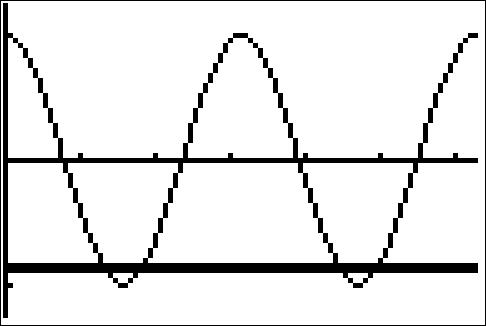
\includegraphics[width=2in]{./IntroTrigGraphics/TrigEquIneq01.jpg} &

\hspace{0.75in} 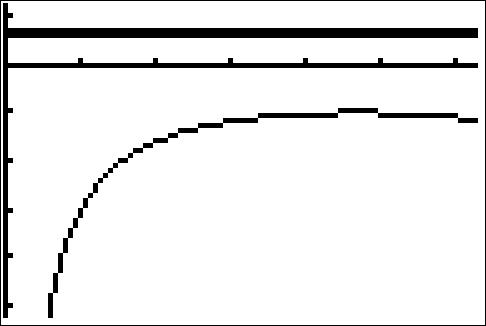
\includegraphics[width=2in]{./IntroTrigGraphics/TrigEquIneq02.jpg} \\

 $y = \cos(2x)$ and  \boldmath $y=-\frac{\sqrt{3}}{2}$ & 

 \hspace{0.75in}  $y = \frac{1}{\sin\left(\frac{1}{3}x-\pi\right)}$ and \boldmath $y =\sqrt{2}$ \\
 
\end{tabular}

\end{center}

\item  Since $\cot(3x) = 0$ has the form $\cot(u) = 0$, we know $u = \frac{\pi}{2} + \pi k$, so, in this case,  $3x =  \frac{\pi}{2} + \pi k$ for integers $k$.  Solving for $x$ yields $x = \frac{\pi}{6} + \frac{\pi}{3} k$.  Checking our answers, we get

\[ \begin{array}{rclr}

\cot\left(3\left[ \frac{\pi}{6} + \frac{\pi}{3} k\right]\right)  &  = &  \cot\left(\frac{\pi}{2} + \pi k\right)  & \\ [3pt]
																												& =  &   \cot\left(\frac{\pi}{2}\right) &  \text{(the period of cotangent is $\pi$)} \\ [3pt]
																												& =  & 0 & \\
																								
\end{array}\] 



 As $k$ runs through the integers, we obtain six answers, corresponding to $k=0$ through $k=5$, which lie in $[0, 2\pi)$: $x = \frac{\pi}{6}$, $\frac{\pi}{2}$, $\frac{5\pi}{6}$, $\frac{7\pi}{6}$ , $\frac{3\pi}{2}$ and  $\frac{11\pi}{6}$. To confirm these graphically, we must be careful. On many calculators, there is no function button for cotangent.  We choose\footnote{The reader is encouraged to see what happens if we had chosen the reciprocal identity $\cot(3x) = \frac{1}{\tan(3x)}$ instead.  The graph on the calculator \textit{appears} identical, but what happens when you try to find the intersection points?} to use the quotient identity  $\cot(3x) = \frac{\cos(3x)}{\sin(3x)}$.  Graphing $y = \frac{\cos(3x)}{\sin(3x)}$ and $y = 0$ (the $x$-axis), we see that the $x$-coordinates of the intersection points approximately match our solutions.

\item The complication in solving an equation like $\sec^{2}(x) = 4$ comes not from the argument of secant, which is just $x$, but rather, the fact the secant is being squared.  To get this equation to look like one of the forms listed on page \pageref{trigeqnstrategy1}, we extract square roots to get $\sec(x) = \pm 2$. Converting to cosines, we have  $\cos(x) = \pm \frac{1}{2}$.  For $\cos(x) = \frac{1}{2}$, we get $x = \frac{\pi}{3} + 2\pi k$ or $x = \frac{5\pi}{3} + 2\pi k$ for integers $k$.  For $\cos(x) = -\frac{1}{2}$, we get $x = \frac{2\pi}{3} + 2\pi k$ or $x = \frac{4\pi}{3} + 2\pi k$ for integers $k$.  If we take a step back and think of these families of solutions geometrically, we see we are finding the measures of all angles with a reference angle of $\frac{\pi}{3}$.  As a result, these solutions can be combined and we may write our solutions as $x = \frac{\pi}{3} + \pi k$ and $x = \frac{2\pi}{3} + \pi k$ for integers $k$.  To check the first family of solutions, we note that, depending on the integer $k$,  $\sec\left(\frac{\pi}{3} + \pi k\right)$ doesn't always equal $\sec\left(\frac{\pi}{3}\right)$.  However, it is true that for all integers $k$,  $\sec\left(\frac{\pi}{3} + \pi k\right) = \pm \sec\left(\frac{\pi}{3}\right) = \pm 2$.  (Can you show this?)  As a result, 


\[ \begin{array}{rclr}

\sec^{2}\left(\frac{\pi}{3} + \pi k\right)  &  = &  \left( \pm \sec\left(\frac{\pi}{3}\right)\right)^2  & \\ [3pt]
																												& =  &   (\pm 2)^2 &  \\ [3pt]
																												& =  & 4 & \\
																								
\end{array}\] 

The same holds for the family $x =\frac{2\pi}{3} + \pi k$.  The solutions which lie in $[0,2\pi)$ come from the values $k = 0$ and $k=1$, namely $x = \frac{\pi}{3}$, $\frac{2\pi}{3}$, $\frac{4\pi}{3}$ and $\frac{5\pi}{3}$.  To confirm graphically, we use a reciprocal identity to rewrite the secant as cosine.  The $x$-coordinates of the intersection points of  $y = \frac{1}{(\cos(x))^2}$ and $y = 4$ verify our answers.


\begin{center}

\begin{tabular}{cc}

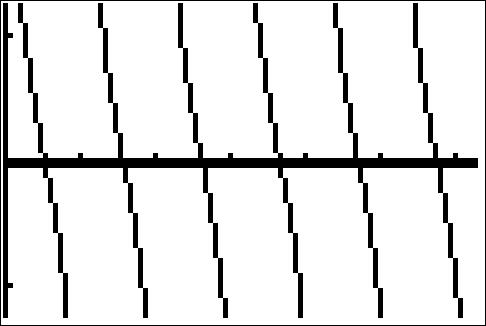
\includegraphics[width=2in]{./IntroTrigGraphics/TrigEquIneq03.jpg} &

\hspace{0.75in} 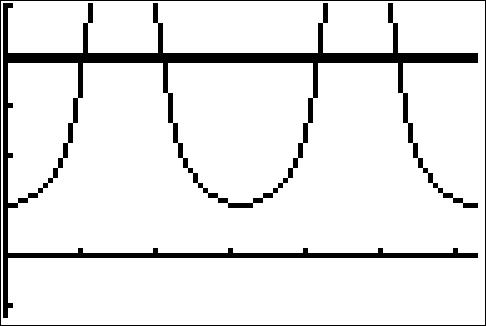
\includegraphics[width=2in]{./IntroTrigGraphics/TrigEquIneq04.jpg} \\

  $y = \frac{\cos(3x)}{\sin(3x)}$ and \boldmath $y=0$   & 

 \hspace{0.75in}   $y = \frac{1}{\cos^{2}(x)}$ and \boldmath $y = 4$  \\

\end{tabular}

\end{center}

\item  The equation  $\tan\left(\frac{x}{2}\right) = -3$ has the form $\tan(u) = -3$, whose solution is $u = \arctan(-3) + \pi k$.  Hence, $\frac{x}{2} = \arctan(-3) + \pi k$, so  $x = 2\arctan(-3) + 2\pi k$ for integers $k$.  To check, we note

\[ \begin{array}{rclr}

\tan\left(\frac{2\arctan(-3) + 2\pi k}{2}\right)  &  = & \tan\left( \arctan(-3) + \pi k \right)  & \\ [3pt]
																												& =  & \tan\left(\arctan(-3) \right) & \text{(the period of tangent is $\pi$)} \\ [3pt]
																												& =  & -3 & (\text{See Theorem } \ref{arctangentcotangentfunctionprops}) \\
																								
\end{array}\] 


 To determine which of our answers lie in the interval $[0,2\pi)$, we first need to get an idea of the value of $2\arctan(-3)$.  While we could easily find an approximation using a calculator,\footnote{Your instructor will let you know if you should abandon the analytic route at this point and use your calculator.  But seriously, what fun would that be?} we proceed analytically.  Since $-3 < 0$, it follows that $-\frac{\pi}{2} < \arctan(-3) < 0$.  Multiplying through by $2$ gives $-\pi < 2\arctan(-3) < 0$.   We are now in a position to argue which of the solutions $x = 2\arctan(-3) + 2\pi k$ lie in $[0,2\pi)$.  For $k = 0$, we get $x = 2\arctan(-3) < 0$, so we discard this answer and all answers $x = 2\arctan(-3) + 2\pi k$ where $k < 0$.  Next, we turn our attention to $k = 1$ and get $x = 2\arctan(-3) + 2\pi$. Starting with the inequality $-\pi < 2\arctan(-3) < 0$, we add $2\pi$  and get $\pi < 2\arctan(-3) +2\pi < 2\pi$.  This means $x = 2\arctan(-3) + 2\pi$ lies in $[0,2\pi)$.  Advancing $k$ to $2$ produces $x = 2\arctan(-3) + 4\pi$. Once again, we get from $-\pi < 2\arctan(-3) < 0$ that $3\pi < 2\arctan(-3) + 4\pi < 4\pi$.  Since this is outside the interval $[0,2\pi)$,  we discard $x = 2\arctan(-3) + 4\pi$ and all solutions of the form $x = 2\arctan(-3) + 2\pi k$ for $k > 2$.   Graphically, we see $y = \tan\left(\frac{x}{2}\right)$ and $y = -3$ intersect only once on $[0,2\pi)$ at $x = 2\arctan(-3) + 2\pi\approx 3.7851$.

\item To solve $\sin(2x) = 0.87$, we first note that it has the form $\sin(u) = 0.87$, which has the family of solutions $u = \arcsin(0.87) + 2\pi k$ or $u =\pi -  \arcsin(0.87) + 2\pi k$ for integers $k$. Since the argument of sine here is $2x$, we get $2x = \arcsin(0.87) + 2\pi k$ or $2x =\pi -  \arcsin(0.87) + 2\pi k$ which gives $x = \frac{1}{2} \arcsin(0.87) + \pi k$ or $x =\frac{\pi}{2} -  \frac{1}{2}\arcsin(0.87) + \pi k$ for integers $k$.  To check,

\[ \begin{array}{rclr}

\sin\left(2\left[\frac{1}{2} \arcsin(0.87) + \pi k\right]\right)  &  = & \sin\left(\arcsin(0.87) + 2\pi k\right)  & \\ [3pt]
																													& =  & \sin\left(\arcsin(0.87)\right) & \text{(the period of sine is $2\pi$)} \\ [3pt]
																												& =  & 0.87& (\text{See Theorem } \ref{arccosinesinefunctionprops})\\
																								
\end{array}\] 


For the family $x =\frac{\pi}{2} -  \frac{1}{2}\arcsin(0.87) + \pi k$ , we get

\[ \begin{array}{rclr}

\sin\left(2\left[\frac{\pi}{2} - \frac{1}{2} \arcsin(0.87) + \pi k\right]\right)  &  = & \sin\left(\pi - \arcsin(0.87) + 2\pi k\right) & \\ [3pt]
																												& =  & \sin\left(\pi - \arcsin(0.87)\right) & \text{(the period of sine is $2\pi$)} \\ [3pt]
																												& =  & \sin\left(\arcsin(0.87)\right) & \text{($\sin(\pi - t) = \sin(t)$)} \\ [3pt]
																												& =  & 0.87& (\text{See Theorem } \ref{arccosinesinefunctionprops}) \\
																								
\end{array}\] 

To determine which of these solutions lie in $[0,2\pi)$, we first need to get an idea of the value of $x=\frac{1}{2} \arcsin(0.87)$.  Once again, we could use the calculator, but we adopt an analytic route here.  By definition, $0 < \arcsin(0.87) < \frac{\pi}{2}$ so that multiplying through by $\frac{1}{2}$ gives us $0 < \frac{1}{2} \arcsin(0.87) < \frac{\pi}{4}$.  Starting with the family of solutions $x = \frac{1}{2} \arcsin(0.87) + \pi k$, we use the same kind of arguments as in our solution to number \ref{arctanin02pi} above and find only the solutions corresponding to $k =0$ and $k=1$ lie in $[0,2\pi)$:  $x = \frac{1}{2} \arcsin(0.87)$ and $x = \frac{1}{2} \arcsin(0.87) + \pi$.  Next, we move to the family $x =\frac{\pi}{2} -  \frac{1}{2}\arcsin(0.87) + \pi k$ for integers $k$. Here, we need to get a better estimate of $\frac{\pi}{2} - \frac{1}{2} \arcsin(0.87)$.  From the inequality $0 < \frac{1}{2}\arcsin(0.87) < \frac{\pi}{4}$, we first multiply through by $-1$ and then add $\frac{\pi}{2}$ to get $\frac{\pi}{2} > \frac{\pi}{2} -\frac{1}{2} \arcsin(0.87) >  \frac{\pi}{4}$, or $\frac{\pi}{4} < \frac{\pi}{2} -\frac{1}{2} \arcsin(0.87) < \frac{\pi}{2}$.  Proceeding with the usual arguments, we find the only solutions which lie in $[0,2\pi)$ correspond to $k = 0$ and $k=1$, namely $x =\frac{\pi}{2} -  \frac{1}{2}\arcsin(0.87)$ and  $x = \frac{3\pi}{2} - \frac{1}{2}\arcsin(0.87)$. All told, we have found four solutions to $\sin(2x) = 0.87$ in $[0,2\pi)$:  $x =\frac{1}{2} \arcsin(0.87)$, $x=\frac{1}{2} \arcsin(0.87) + \pi$, $x =\frac{\pi}{2} -  \frac{1}{2}\arcsin(0.87)$ and  $x = \frac{3\pi}{2} - \frac{1}{2}\arcsin(0.87)$. By graphing $y = \sin(2x)$ and $y = 0.87$, we confirm our results.

\enlargethispage*{.5in}

\begin{center}

\begin{tabular}{cc}

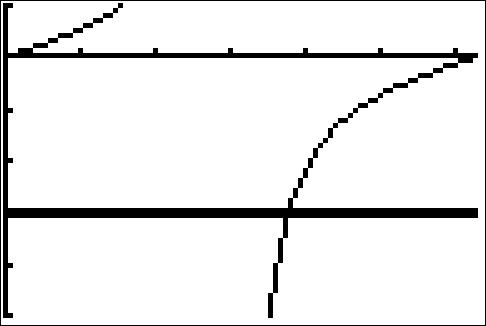
\includegraphics[width=2in]{./IntroTrigGraphics/TrigEquIneq05.jpg} &

\hspace{0.75in} 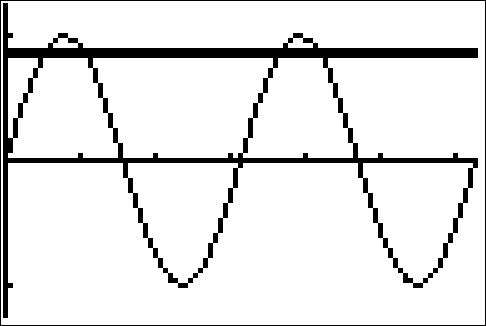
\includegraphics[width=2in]{./IntroTrigGraphics/TrigEquIneq06.jpg} \\

$y = \tan\left(\frac{x}{2}\right)$ and \boldmath $y = -3$    & 

 \hspace{0.75in}  $y = \sin(2x)$ and \boldmath $y = 0.87$ \\

\end{tabular}

\end{center} 

\end{enumerate}

\vspace*{-.3in} \qed

\end{ex}

\pagebreak

Each of the problems in Example \ref{TrigEqnEx1} featured one trigonometric function.  If an equation involves two different trigonometric functions or if the equation contains the same trigonometric function but with different arguments, we will need to use identities and Algebra to reduce the equation to the same form as those given on page  \pageref{trigeqnstrategy1}.
 
\begin{ex} \label{TrigEqIdEx1}  Solve the following equations and list the solutions which lie in the interval $[0,2\pi)$.  Verify your solutions on $[0,2\pi)$ graphically.

\begin{multicols}{2}

\begin{enumerate}

\item  $3\sin^{3}(x) = \sin^{2}(x)$
\item $\sec^{2}(x) = \tan(x) + 3$

\setcounter{HW}{\value{enumi}}

\end{enumerate}

\end{multicols}

\begin{multicols}{2}

\begin{enumerate}

\setcounter{enumi}{\value{HW}}

\item   $\cos(2x) = 3\cos(x) - 2$
\item  $\cos(3x) = 2- \cos(x)$

\setcounter{HW}{\value{enumi}}

\end{enumerate}

\end{multicols}

\begin{multicols}{2}

\begin{enumerate}

\setcounter{enumi}{\value{HW}}

\item  $\cos(3x) = \cos(5x)$
\item $\sin(2x) =\sqrt{3} \cos(x)$

\setcounter{HW}{\value{enumi}}

\end{enumerate}

\end{multicols}

\begin{multicols}{2}

\begin{enumerate}

\setcounter{enumi}{\value{HW}}

\item  $\sin(x)\cos\left(\frac{x}{2}\right) + \cos(x)\sin\left(\frac{x}{2}\right) = 1$
\item  $\cos(x) - \sqrt{3} \sin(x) = 2$

\end{enumerate}
 
\end{multicols}

{\bf Solution.}

\begin{enumerate}

\item We resist the temptation to divide both sides of $3\sin^{3}(x) = \sin^{2}(x)$ by $\sin^{2}(x)$ (What goes wrong if you do?) and instead gather all of the terms to one side of the equation and factor.

\[ \begin{array}{rclr}

3\sin^{3}(x) & = &  \sin^{2}(x) & \\
3\sin^{3}(x) -  \sin^{2}(x) & = & 0 &  \\
\sin^{2}(x) (3 \sin(x) - 1) & = & 0 & \text{Factor out $\sin^{2}(x)$ from both terms.} \\ \end{array} \]

We get $\sin^{2}(x) = 0$ or $3\sin(x) - 1 = 0$. Solving for $\sin(x)$, we find  $\sin(x) = 0$ or $\sin(x) = \frac{1}{3}$.  The solution to the first equation is $x = \pi k$, with $x = 0$ and $x = \pi$ being the two solutions which lie in $[0,2\pi)$.  To solve $\sin(x) = \frac{1}{3}$, we use the arcsine function to get $x = \arcsin\left(\frac{1}{3}\right) + 2\pi k$ or $x = \pi - \arcsin\left(\frac{1}{3}\right) + 2\pi k$ for integers $k$. We find the two solutions here which lie in $[0,2\pi)$ to be $x = \arcsin\left(\frac{1}{3}\right)$ and $x = \pi - \arcsin\left(\frac{1}{3}\right)$.  To check graphically, we plot $y = 3(\sin(x))^3$ and $y = (\sin(x))^2$ and find the  $x$-coordinates of the intersection points of these two curves.  Some extra zooming is required near $x=0$ and $x=\pi$ to verify that these two curves do in fact intersect four times.\footnote{Note that we are \textit{not} counting the point $(2\pi,0)$ in our solution set since $x = 2\pi$ is not in the interval $[0,2\pi)$. In the forthcoming solutions, remember that while  $x = 2\pi$ may be a solution to the equation, it isn't counted among the solutions in $[0,2\pi)$.}

\item  Analysis of  $\sec^{2}(x) = \tan(x) + 3$ reveals two different trigonometric functions, so an identity is in order.  Since $\sec^{2}(x) = 1 + \tan^{2}(x)$, we get

\[ \begin{array}{rclr}

\sec^{2}(x) &  = & \tan(x) + 3 & \\
1 + \tan^{2}(x) & = & \tan(x) + 3& \text{(Since $\sec^{2}(x) = 1 + \tan^{2}(x)$.)} \\
\tan^{2}(x) - \tan(x) -2 & = & 0 & \\
u^2 - u - 2 & = & 0 & \text{Let $u = \tan(x)$.} \\
(u + 1)(u - 2) & = & 0 & \\ \end{array} \]

This gives $u = -1$ or $u = 2$.  Since $u = \tan(x)$, we have $\tan(x) = -1$ or $\tan(x) = 2$. From $\tan(x) = -1$, we get $x = -\frac{\pi}{4} + \pi k$ for integers $k$.  To solve $\tan(x) = 2$, we employ the arctangent function and get $x = \arctan(2) + \pi k$ for integers $k$.  From the first set of solutions, we get $x = \frac{3\pi}{4}$ and $x = \frac{7\pi}{4}$ as our answers which lie in $[0,2\pi)$.  Using the same sort of argument we saw in Example \ref{TrigEqnEx1},   we get  $x=\arctan(2)$ and $x = \pi + \arctan(2)$ as answers from our second set of solutions which lie in $[0,2\pi)$.  Using a reciprocal identity, we rewrite the secant as a cosine and graph  $y = \frac{1}{(\cos(x))^2}$ and $y = \tan(x) + 3$ to find the $x$-values of the points where they intersect.


\begin{center}

\begin{tabular}{cc}

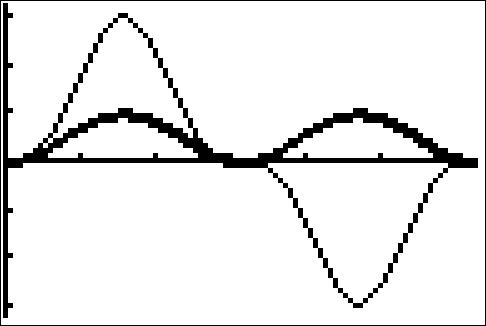
\includegraphics[width=2in]{./IntroTrigGraphics/TrigEquIneq07.jpg} &

\hspace{0.75in} 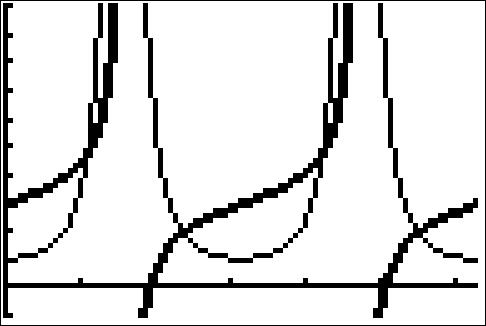
\includegraphics[width=2in]{./IntroTrigGraphics/TrigEquIneq08.jpg} \\

$y = 3(\sin(x))^3$ and \boldmath  $y = (\sin(x))^2$   & 

 \hspace{0.75in} $y = \frac{1}{(\cos(x))^2}$ and \boldmath  $y = \tan(x) + 3$  \\
 
 \end{tabular}

\end{center}

\item  In the equation $\cos(2x) = 3\cos(x) - 2$, we have the same circular function, namely cosine, on both sides but the arguments differ.  Using the identity $\cos(2x) = 2\cos^{2}(x) - 1$, we obtain a `quadratic in disguise' and proceed as we have done in the past.

\[ \begin{array}{rclr}

\cos(2x) & = & 3\cos(x) - 2 & \\
2\cos^{2}(x) -1 & = & 3\cos(x) -2 & \text{(Since $\cos(2x) = 2\cos^{2}(x) -1$.)} \\
2\cos^{2}(x) - 3\cos(x) +1 & = & 0 & \\
2 u^2 - 3 u + 1 & = & 0 & \text{Let $u = \cos(x)$.}\\
(2u - 1)(u - 1) & = & 0 & \\ \end{array} \]

This gives $u = \frac{1}{2}$ or $u = 1$.  Since $u = \cos(x)$, we get $\cos(x) = \frac{1}{2}$ or $\cos(x) = 1$.  Solving  $\cos(x) = \frac{1}{2}$, we get $x = \frac{\pi}{3} + 2\pi k$ or $x = \frac{5\pi}{3} + 2\pi k$ for integers $k$.  From $\cos(x) = 1$, we get $x = 2\pi k$ for integers $k$.  The answers which lie in $[0,2\pi)$ are $x =0$,  $\frac{\pi}{3}$, and $\frac{5\pi}{3}$.  Graphing $y = \cos(2x)$ and $y = 3\cos(x) - 2$, we find, after a little extra effort, that the curves intersect in three places on $[0,2\pi)$, and  the $x$-coordinates of these points confirm our results.


\item  To solve $\cos(3x) = 2- \cos(x)$, we use the same technique as in the previous problem.  From Example \ref{doubleangleex}, number \ref{cosinepolynomial}, we know that $\cos(3x) = 4\cos^{3}(x) - 3\cos(x)$.  This transforms the equation into a polynomial in terms of $\cos(x)$.


\[ \begin{array}{rclr}

\cos(3x) & = &2- \cos(x) & \\
4\cos^{3}(x) - 3\cos(x) & = & 2- \cos(x) & \\
2\cos^{3}(x) - 2\cos(x) -2  & = & 0 & \\
4 u^3 - 2 u -2  & = & 0 & \text{Let $u = \cos(x)$.} \\ \end{array} \]

To solve $4u^3-2u-2=0$, we need the techniques in Chapter \ref{Polynomials} to factor $4u^3-2u-2$ into $(u-1)\left(4u^2+4u+2\right)$.  We get either $u-1 = 0$ or  $4u^2+2u+2=0$, and since the discriminant of the latter is negative, the only real solution to $4u^3-2u-2=0$ is $u = 1$.  Since $u = \cos(x)$, we get $\cos(x) = 1$, so $x = 2\pi k$ for integers $k$.  The only solution which lies in $[0,2\pi)$ is $x = 0$.  Graphing $y = \cos(3x)$ and $y = 2- \cos(x)$ on the same set of axes over $[0,2\pi)$ shows that the graphs intersect at what appears to be $(0,1)$, as required.

\begin{center}

\begin{tabular}{cc}

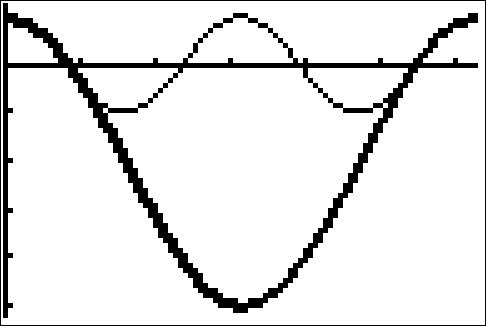
\includegraphics[width=2in]{./IntroTrigGraphics/TrigEquIneq09.jpg} &

\hspace{0.75in} 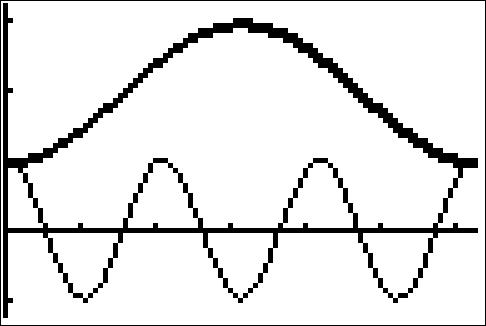
\includegraphics[width=2in]{./IntroTrigGraphics/TrigEquIneq10.jpg} \\

$y = \cos(2x)$ and \boldmath  $y = 3\cos(x) - 2$   & 

 \hspace{0.75in} $y = \cos(3x)$ and \boldmath $y = 2- \cos(x)$ \\
 
 \end{tabular}

\end{center}


\item  While we could approach  $\cos(3x) = \cos(5x)$ in the same manner as we did the previous two problems, we choose instead to showcase the utility of the Sum to Product Identities.  From $\cos(3x) = \cos(5x)$, we get $\cos(5x) - \cos(3x) = 0$, and it is the presence of $0$ on the right hand side that indicates a switch to a product would be a good move.\footnote{As always, experience is the greatest teacher here!}  Using Theorem \ref{sumtoproduct}, we have that $\cos(5x) - \cos(3x)  = - 2 \sin\left( \frac{5x + 3x}{2}\right)\sin\left( \frac{5x - 3x}{2}\right) = -2 \sin(4x)\sin(x)$.  Hence, the equation $\cos(5x) = \cos(3x)$ is equivalent to $-2 \sin(4x) \sin(x) = 0$.  From this, we get $\sin(4x) = 0$ or $\sin(x)$ = 0.  Solving $\sin(4x) = 0$ gives $x = \frac{\pi}{4} k$ for integers $k$, and the solution to $\sin(x) = 0$ is $x = \pi k$ for integers $k$.  The second set of solutions is contained in the first set of solutions,\footnote{As always, when in doubt, write it out!} so our final solution to $\cos(5x) = \cos(3x)$ is $x = \frac{\pi}{4} k$ for integers $k$.  There are eight of these answers which lie in $[0,2\pi)$:  $x = 0$, $\frac{\pi}{4}$, $\frac{\pi}{2}$, $\frac{3\pi}{4}$, $\pi$, $\frac{5\pi}{4}$, $\frac{3\pi}{2}$ and $\frac{7\pi}{4}$.  Our plot of the graphs of $y = \cos(3x)$ and $y = \cos(5x)$ below (after some careful zooming) bears this out. 

\item  In examining the equation   $\sin(2x) =\sqrt{3} \cos(x)$, not only do we have different circular functions involved, namely sine and cosine, we also have different arguments to contend with, namely $2x$ and $x$.  Using the identity $\sin(2x) = 2 \sin(x) \cos(x)$ makes all of the arguments the same and we proceed as we would solving any nonlinear equation -- gather all of the nonzero terms on one side of the equation and factor.

\[ \begin{array}{rclr}

\sin(2x) & = & \sqrt{3} \cos(x) & \\
2 \sin(x) \cos(x) & = & \sqrt{3} \cos(x)  & \text{(Since $\sin(2x) = 2\sin(x) \cos(x)$.)} \\
2\sin(x) \cos(x) - \sqrt{3} \cos(x) & = & 0 & \\
\cos(x) (2 \sin(x) - \sqrt{3}) & = & 0 & \\ \end{array} \]

from which we get $\cos(x) = 0$ or $\sin(x) = \frac{\sqrt{3}}{2}$. From $\cos(x) = 0$, we obtain $x = \frac{\pi}{2} + \pi k$ for integers $k$. From $\sin(x) = \frac{\sqrt{3}}{2}$, we get $x = \frac{\pi}{3} + 2\pi k$ or $x = \frac{2\pi}{3} + 2\pi k$ for integers $k$.  The answers which lie in $[0,2\pi)$ are $x = \frac{\pi}{2}$, $\frac{3\pi}{2}$, $\frac{\pi}{3}$ and $\frac{2\pi}{3}$.  We graph $y = \sin(2x)$ and $y = \sqrt{3} \cos(x)$ and, after some careful zooming,  verify our answers.

\begin{center}

\begin{tabular}{cc}

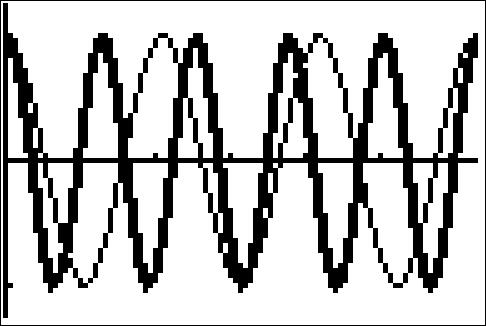
\includegraphics[width=2in]{./IntroTrigGraphics/TrigEquIneq11.jpg} &

\hspace{0.75in} 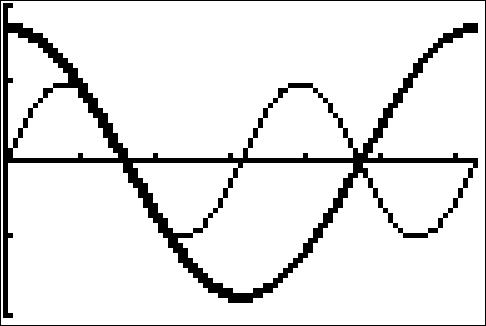
\includegraphics[width=2in]{./IntroTrigGraphics/TrigEquIneq12.jpg} \\

$y = \cos(3x)$ and \boldmath $y = \cos(5x)$    & 

 \hspace{0.75in} $y = \sin(2x)$ and \boldmath $y = \sqrt{3} \cos(x)$  \\
 
 \end{tabular}

\end{center}

\item Unlike the previous problem, there seems to be no quick way to get the circular functions or their arguments to match in the equation $\sin(x)\cos\left(\frac{x}{2}\right) + \cos(x)\sin\left(\frac{x}{2}\right) = 1$.  If we stare at it long enough, however,  we realize that the left hand side is the expanded form of the sum formula for $\sin\left(x + \frac{x}{2}\right)$.  Hence, our original equation is equivalent to  $\sin\left(\frac{3}{2} x\right) = 1$.  Solving, we find $x = \frac{\pi}{3} + \frac{4\pi}{3} k$ for integers $k$.  Two of these solutions lie in $[0,2\pi)$: $x = \frac{\pi}{3}$ and $x = \frac{5\pi}{3}$. Graphing $y = \sin(x)\cos\left(\frac{x}{2}\right) + \cos(x)\sin\left(\frac{x}{2}\right)$ and $y = 1$ validates our solutions.

\item  With the absence of double angles or squares, there doesn't seem to be much we can do.  However, since the arguments of the cosine and sine are the same, we can rewrite the left hand side of this equation as a sinusoid.\footnote{We are essentially `undoing' the sum / difference formula for cosine or sine, depending on which form we use, so this problem is actually closely related to the previous one!}  To fit $f(x) = \cos(x) - \sqrt{3} \sin(x)$ to the form $A\sin(\omega t + \phi) + B$, we use what we learned in Example \ref{expandedsinusoidex1} and find $A = 2$, $B = 0$, $\omega = 1$ and $\phi = \frac{5\pi}{6}$.   Hence, we can rewrite the equation  $\cos(x) - \sqrt{3} \sin(x) = 2$  as $2 \sin\left(x + \frac{5\pi}{6}\right) = 2$, or $\sin\left(x + \frac{5\pi}{6}\right) = 1$.  Solving the latter, we get $x  = - \frac{\pi}{3} + 2\pi k$ for integers $k$. Only one of these solutions, $x = \frac{5\pi}{3}$, which corresponds to $k=1$, lies in $[0,2\pi)$.  Geometrically, we see that $y = \cos(x) - \sqrt{3} \sin(x)$ and $y = 2$ intersect just once, supporting our answer.

\begin{center}

\begin{tabular}{cc}

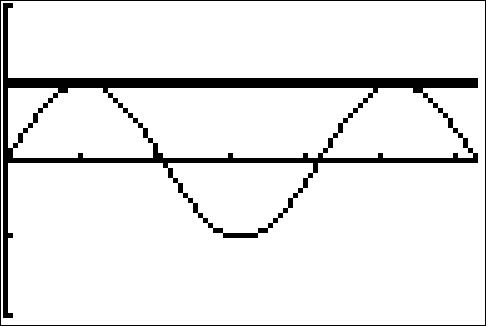
\includegraphics[width=2in]{./IntroTrigGraphics/TrigEquIneq13.jpg} &

\hspace{0.25in} 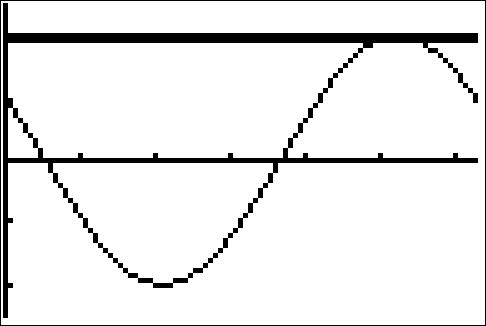
\includegraphics[width=2in]{./IntroTrigGraphics/TrigEquIneq14.jpg} \\

$y = \sin(x)\cos\left(\frac{x}{2}\right) + \cos(x)\sin\left(\frac{x}{2}\right)$ and \boldmath $y = 1$     & 

 \hspace{0.25in}  $y = \cos(x) - \sqrt{3} \sin(x)$ and \boldmath $y = 2$ \\

\end{tabular}

\end{center}

\end{enumerate}
\vspace{-.25in} \qed
\end{ex}
 
We repeat here the advice given when solving systems of nonlinear equations in section \ref{NonLinear} --  when it comes to solving equations involving the trigonometric functions, it helps to just try something.  

Next, we focus on solving inequalities involving the trigonometric functions.  Since these functions are continuous on their domains, we may use the sign diagram technique we've used in the past to solve the inequalities.\footnote{See page \pageref{firstsigndiagram}, Example \ref{polygraphex}, page \pageref{rationalsigndiagram}, page \pageref{algebraicsigndiagram}, Example \ref{expineq} and Example \ref{logineq} for discussion of this technique.}

\begin{ex}  \label{TrigIneqEx1} Solve the following inequalities on $[0,2\pi)$.  Express your answers using interval notation and verify your answers graphically.

\begin{multicols}{3}

\begin{enumerate}

\item  $2\sin(x) \leq 1$

\item  $\sin(2x) > \cos(x)$

\item  $\tan(x) \geq 3$

\end{enumerate}

\end{multicols}

{\bf Solution.}

\begin{enumerate}

\item  We begin solving $2\sin(x) \leq 1$ by collecting all of the terms on one side of the equation and zero on the other to get $2\sin(x) - 1 \leq 0$.  Next, we let $f(x) = 2\sin(x) - 1$ and note that our original inequality is equivalent to solving $f(x) \leq 0$. We now look to see where, if ever, $f$ is undefined and where $f(x) = 0$.  Since the domain of $f$ is all real numbers, we can immediately set  about finding the zeros of $f$.  Solving $f(x) = 0$, we have $2\sin(x) - 1=0$ or $\sin(x) = \frac{1}{2}$.  The solutions here are $x = \frac{\pi}{6} + 2\pi k$ and $x = \frac{5\pi}{6} + 2\pi k$ for integers $k$.  Since we are restricting our attention to $[0,2\pi)$, only $x = \frac{\pi}{6}$ and $x = \frac{5\pi}{6}$ are of concern to us.  Next, we choose test values in $[0,2\pi)$ other than the zeros and determine if $f$ is positive or negative there.  For $x = 0$ we have $f(0) = -1$, for $x = \frac{\pi}{2}$ we get $f\left(\frac{\pi}{2}\right) = 1$ and for $x = \pi$ we get $f(\pi) = -1$.  Since our original inequality is equivalent to $f(x) \leq 0$, we are looking for where the function is negative $(-)$ or $0$, and we get the intervals $\left[0, \frac{\pi}{6}\right] \cup \left[\frac{5\pi}{6}, 2\pi \right)$.  We can confirm our answer graphically by seeing where the graph of $y = 2\sin(x)$ crosses or is below the graph of $y = 1$. 

\begin{center}

\begin{tabular}{m{2in}c}

\begin{mfpic}[10]{-6}{6}{-2}{2}
\polyline{(-6,0),(6,0)}
\xmarks{-6,-2,2,6}
\tiny
\tlpointsep{6pt}
\normalsize
\tlabel[cc](-6,-1){$0$}
\tlabel[cc](-4,1){$(-)$}
\tlabel[cc](-2,-1){$\frac{\pi}{6}$}
\tlabel[cc](-2,1){0}
\tlabel[cc](0,1){$(+)$}
\tlabel[cc](2,-1){$\frac{5\pi}{6}$}
\tlabel[cc](2,1){$0$}
\tlabel[cc](4,1){$(-)$}
\tlabel[cc](6,-1){$2\pi$}
\end{mfpic} 

& 

\hspace{.75in} 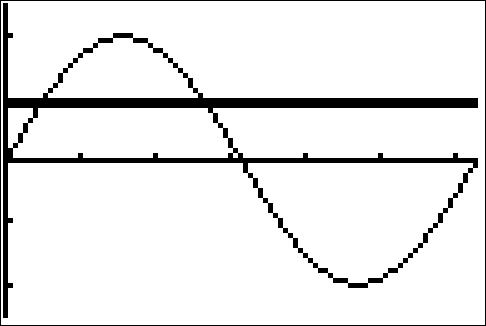
\includegraphics[width=2in]{./IntroTrigGraphics/TrigEquIneq15.jpg} \\

& \hspace{.75in} $y = 2\sin(x)$ and \boldmath $y = 1$ \\

\end{tabular}

\end{center}


\item  We first rewrite  $\sin(2x) > \cos(x)$   as $\sin(2x) - \cos(x) > 0$ and let $f(x) = \sin(2x) - \cos(x)$.  Our original inequality is thus equivalent to $f(x) > 0$. The domain of $f$ is all real numbers, so we can advance to finding the zeros of $f$.  Setting $f(x) = 0$ yields $\sin(2x) - \cos(x) = 0$, which, by way of the double angle identity for sine, becomes $2\sin(x)\cos(x) - \cos(x) = 0$ or $\cos(x) (2\sin(x) - 1) = 0$.  From $\cos(x) = 0$, we get $x = \frac{\pi}{2} + \pi k$ for integers $k$ of which only $x = \frac{\pi}{2}$ and $x = \frac{3\pi}{2}$ lie in $[0,2\pi)$.  For $2\sin(x) - 1 = 0$, we get $\sin(x) = \frac{1}{2}$ which gives $x = \frac{\pi}{6} + 2\pi k$ or $x = \frac{5\pi}{6} + 2\pi k$ for integers $k$.  Of those, only $x = \frac{\pi}{6}$ and $x = \frac{5\pi}{6}$ lie in $[0,2\pi)$.  Next, we choose our test values.  For $x =0$ we find $f(0) = -1$; when $x = \frac{\pi}{4}$ we get $f\left(\frac{\pi}{4}\right) =1 - \frac{\sqrt{2}}{2} = \frac{2 - \sqrt{2}}{2}$;  for $x = \frac{3\pi}{4}$ we get $f\left(\frac{3\pi}{4}\right) =-1 + \frac{\sqrt{2}}{2} =  \frac{\sqrt{2} - 2}{2}$;  when $x=\pi$ we have $f(\pi) = 1$, and lastly, for $x = \frac{7\pi}{4}$ we get $f\left(\frac{7\pi}{4}\right) = -1 - \frac{\sqrt{2}}{2} =  \frac{-2 - \sqrt{2}}{2}$.  We see $f(x) > 0$ on $\left(\frac{\pi}{6}, \frac{\pi}{2}\right) \cup \left(\frac{5\pi}{6}, \frac{3\pi}{2}\right)$, so this is our answer.  We can use the calculator to check that the graph of $y = \sin(2x)$ is indeed above the graph of $y = \cos(x)$ on those intervals. 

\begin{center}
\begin{tabular}{m{2in}c}

\begin{mfpic}[10]{-10}{10}{-2}{2}
\polyline{(-10,0),(10,0)}
\xmarks{-10,-6,-2,2,6,10}
\tiny
\tlpointsep{6pt}
\normalsize
\tlabel[cc](-10,-1){$0$}
\tlabel[cc](-8,1){$(-)$}
\tlabel[cc](-6,-1){$\frac{\pi}{6}$}
\tlabel[cc](-6,1){0}
\tlabel[cc](-4,1){$(+)$}
\tlabel[cc](-2,-1){$\frac{\pi}{2}$}
\tlabel[cc](-2,1){0}
\tlabel[cc](0,1){$(-)$}
\tlabel[cc](2,-1){$\frac{5\pi}{6}$}
\tlabel[cc](2,1){0}
\tlabel[cc](4,1){$(+)$}
\tlabel[cc](6,-1){$\frac{3\pi}{2}$}
\tlabel[cc](6,1){0}
\tlabel[cc](8,1){$(-)$}
\tlabel[cc](10,-1){$2\pi$}
\end{mfpic} 

& 

\hspace{1.25in} 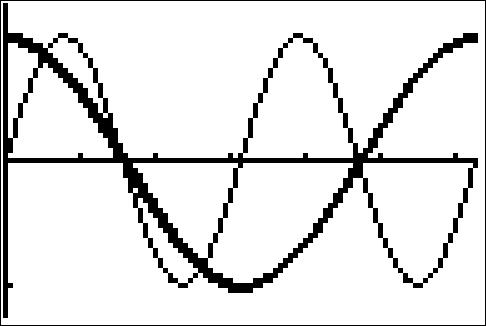
\includegraphics[width=2in]{./IntroTrigGraphics/TrigEquIneq16.jpg} \\

& \hspace{1.25in} $y = \sin(2x)$ and \boldmath $y = \cos(x)$ \\

\end{tabular}

\end{center}

\item  Proceeding as in the last two problems, we rewrite  $\tan(x) \geq 3$ as $\tan(x) - 3 \geq 0$ and let $f(x) = \tan(x) - 3$.  We note that on $[0,2\pi)$, $f$ is undefined at $x =\frac{\pi}{2}$ and $\frac{3\pi}{2}$, so those values will need the usual disclaimer on the sign diagram.\footnote{See page \pageref{rationalsigndiagram} for a discussion of the non-standard character known as the interrobang.}  Moving along to zeros, solving $f(x) = \tan(x) - 3 = 0$ requires the arctangent function.  We find $x = \arctan(3) + \pi k$ for integers $k$ and of these, only $x = \arctan(3)$ and $x = \arctan(3) + \pi$ lie in $[0,2\pi)$.  Since $3 > 0$, we know $0 < \arctan(3) < \frac{\pi}{2}$ which allows us to position these zeros correctly on the sign diagram. To choose test values, we begin with $x=0$ and find $f(0) = -3$. Finding a convenient test value in the interval $\left(\arctan(3), \frac{\pi}{2}\right)$ is a bit more challenging.  Keep in mind that the arctangent function is increasing and is bounded above by $\frac{\pi}{2}$.  This means that the number $x = \arctan(117)$ is guaranteed\footnote{We could have chosen any value $\arctan(t)$ where $t > 3$.} to lie between  $\arctan(3)$ and $\frac{\pi}{2}$.  We see that $f(\arctan(117)) = \tan(\arctan(117)) - 3 = 114$.  For our next test value, we take $x = \pi$ and find $f(\pi) = -3$.  To find our next test value, we note that since $\arctan(3) < \arctan(117) < \frac{\pi}{2}$,  it follows\footnote{\ldots by adding $\pi$ through the inequality \ldots} that $\arctan(3) + \pi < \arctan(117) + \pi < \frac{3\pi}{2}$.  Evaluating $f$ at $x = \arctan(117) + \pi$ yields $f(\arctan(117)+\pi) = \tan(\arctan(117) + \pi) -3 = \tan(\arctan(117)) - 3 = 114$.  We choose our last test value to be $x = \frac{7\pi}{4}$ and find $f\left(\frac{7\pi}{4}\right) = -4$.  Since we want $f(x) \geq 0$, we see that our answer is $\left[ \arctan(3), \frac{\pi}{2}\right) \cup  \left[\arctan(3)+\pi, \frac{3\pi}{2}\right)$.  Using the graphs of $y = \tan(x)$ and $y = 3$, we see when the graph of the former is above (or meets) the graph of the latter.

\begin{center}
\begin{tabular}{m{2in}c}

\begin{mfpic}[10]{-10}{10}{-2}{2}
\polyline{(-10,0),(10,0)}
\xmarks{-10,-6,-2,2,6,10}
\tiny
\tlpointsep{6pt}
\normalsize
\tlabel[cc](-10,-1){$0$}
\tlabel[cc](-8,1){$(-)$}
\tlabel[cc](-6,-1){\tiny $\arctan(3)$}
\tlabel[cc](-6,1){0}
\tlabel[cc](-4,1){$(+)$}
\tlabel[cc](-2,-1){$\frac{\pi}{2}$}
\tlabel[cc](-2,1){\textinterrobang}
\tlabel[cc](0,1){$(-)$}
\tlabel[cc](2,-1){\tiny $(\arctan(3)+\pi)$}
\tlabel[cc](2,1){0}
\tlabel[cc](4,1){$(+)$}
\tlabel[cc](6,-1){$\frac{3\pi}{2}$}
\tlabel[cc](6,1){\textinterrobang}
\tlabel[cc](8,1){$(-)$}
\tlabel[cc](10,-1){$2\pi$}
\end{mfpic} 

& 

\hspace{1.25in} 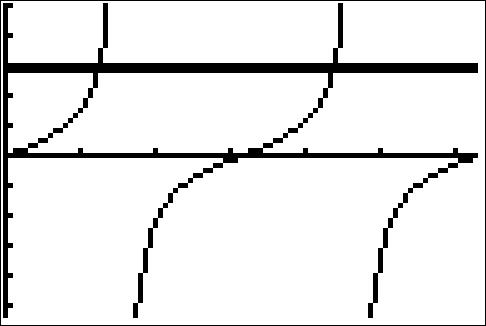
\includegraphics[width=2in]{./IntroTrigGraphics/TrigEquIneq17.jpg} \\

& \hspace{1.25in} $y = \tan(x)$ and \boldmath $y =3$ \\

\end{tabular}

\end{center}


\vspace{-.25in} \qed

\end{enumerate}


\end{ex}


Our next example puts solving equations and inequalities to good use -- finding domains of functions.


\begin{ex}  \label{TrigDomainEx1} Express the domain of the following functions using extended interval notation.\footnote{See page \pageref{extendedinterval} for details about this notation.}

\begin{multicols}{3}

\begin{enumerate}

\item  $f(x) = \csc\left(2x + \frac{\pi}{3}\right)$

\item  $f(x) = \dfrac{\sin(x)}{2\cos(x) - 1}$

\item  $f(x) = \sqrt{1 - \cot(x)}$

\end{enumerate}

\end{multicols}

{\bf Solution.}

\begin{enumerate}

\item  To find the domain of $f(x) = \csc\left(2x + \frac{\pi}{3}\right)$, we rewrite $f$ in terms of sine as $f(x) = \frac{1}{\sin\left(2x + \frac{\pi}{3}\right)}$.  Since the sine function is defined everywhere, our only concern comes from zeros in the denominator.  Solving $\sin\left(2x + \frac{\pi}{3}\right) = 0$, we get $x = -\frac{\pi}{6} + \frac{\pi}{2} k$ for integers $k$.  In set-builder notation, our domain is  $\left\{ x : x \neq  -\frac{\pi}{6} + \frac{\pi}{2} k \, \text{for integers $k$} \right\}$.  To help visualize the domain,  we follow the old mantra `When in doubt, write it out!' We get $\left\{ x : x \neq  -\frac{\pi}{6}, \frac{2\pi}{6}, -\frac{4\pi}{6}, \frac{5\pi}{6}, -\frac{7\pi}{6}, \frac{8\pi}{6}, \ldots \right\}$, where we have kept the denominators $6$ throughout to help see the pattern.  Graphing the situation on a numberline, we have

\begin{center}

\begin{mfpic}[15]{-6}{6}{-1}{2}
\arrow \reverse \arrow \polyline{(-6,0), (6,0)}
\xmarks{-5,-3,-1,1,3,5}
\tlpointsep{5pt}
\axislabels {x}{{\small $-\frac{7\pi}{6} \hspace{7pt}$} -5,{\small $-\frac{4\pi}{6} \hspace{7pt}$} -3, {\small $-\frac{\pi}{6} \hspace{7pt}$} -1,{\small $\frac{2\pi}{6}$} 1,{\small $\frac{5\pi}{6}$} 3,  {\small $\frac{8\pi}{6}$} 5}

\penwd{1.5}
\arrow \reverse \arrow \polyline{(-5.75,1), (5.75,1)}

\penwd{0.75}

\gclear \circle{(-5,1),0.15}
\circle{(-5,1),0.15}

\gclear \circle{(-3,1),0.15}
\circle{(-3,1),0.15}

\gclear \circle{(-1,1),0.15}
\circle{(-1,1),0.15}

\gclear \circle{(5,1),0.15}
\circle{(5,1),0.15}

\gclear \circle{(3,1),0.15}
\circle{(3,1),0.15}

\gclear \circle{(1,1),0.15}
\circle{(1,1),0.15}

\end{mfpic}

\end{center}

Proceeding as we did on page \pageref{extendedinterval} in Section \ref{circularfunctionsbeyond}, we let $x_{\mbox{\tiny $k$}}$ denote the $k$th number excluded from the domain and we have  $x_{\mbox{\tiny $k$}} = -\frac{\pi}{6} + \frac{\pi}{2} k = \frac{(3k-1)\pi}{6}$ for integers $k$.  The intervals which comprise the domain are of the form $\left(x_{\mbox{\tiny $k$}}, x_{\mbox{\tiny $k+1$}}  \right) = \left(\frac{(3k-1)\pi}{6}, \frac{(3k+2)\pi}{6} \right)$ as $k$ runs through the integers.  Using extended interval notation, we have that the domain is

\[ \bigcup_{k = -\infty}^{\infty}  \left(\dfrac{(3k-1)\pi}{6}, \dfrac{(3k+2)\pi}{6} \right)\]

We can check our answer by substituting in values of $k$ to see that it matches our diagram.


\item  Since the domains of $\sin(x)$ and $\cos(x)$ are all real numbers, the only concern when finding the domain of  $f(x) =  \frac{\sin(x)}{2\cos(x) - 1}$ is division by zero so we set the denominator equal to zero and solve. From $2\cos(x) - 1 = 0$ we get $\cos(x) = \frac{1}{2}$ so that $x = \frac{\pi}{3} + 2\pi k$ or $x = \frac{5\pi}{3} + 2\pi k$ for integers $k$.  Using set-builder notation, the domain is $\left\{ x : x \neq \frac{\pi}{3} + 2\pi k \, \text{and} \, x \neq \frac{5\pi}{3} + 2\pi k \, \text{for integers $k$} \right\}$, or  $\left\{ x : x \neq \pm \frac{\pi}{3}, \pm \frac{5\pi}{3}, \pm \frac{7\pi}{3}, \pm \frac{11\pi}{3}, \ldots \right\}$, so we have

\begin{center}

\begin{mfpic}[15]{-6}{6}{-1}{2}
\arrow \reverse \arrow \polyline{(-8,0), (8,0)}
\xmarks{-7,-5,-3,-1,1,3,5,7}
\tlpointsep{5pt}
\axislabels {x}{{\small $-\frac{11\pi}{3} \hspace{7pt}$} -7,{\small $-\frac{7\pi}{3} \hspace{7pt}$} -5,{\small $-\frac{5\pi}{3} \hspace{7pt}$} -3, {\small $-\frac{\pi}{3} \hspace{7pt}$} -1,{\small $\frac{\pi}{3}$} 1,{\small $\frac{5\pi}{3}$} 3,  {\small $\frac{7\pi}{3}$} 5,  {\small $\frac{11\pi}{3}$} 7}

\penwd{1.5}
\arrow \reverse \arrow \polyline{(-7.75,1), (7.75,1)}

\penwd{0.75}

\gclear \circle{(-7,1),0.15}
\circle{(-7,1),0.15}

\gclear \circle{(-5,1),0.15}
\circle{(-5,1),0.15}

\gclear \circle{(-3,1),0.15}
\circle{(-3,1),0.15}

\gclear \circle{(-1,1),0.15}
\circle{(-1,1),0.15}

\gclear \circle{(7,1),0.15}
\circle{(7,1),0.15}

\gclear \circle{(5,1),0.15}
\circle{(5,1),0.15}

\gclear \circle{(3,1),0.15}
\circle{(3,1),0.15}

\gclear \circle{(1,1),0.15}
\circle{(1,1),0.15}


\end{mfpic}

\end{center}

Unlike the previous example, we have \textit{two} different families of points to consider, and we present two ways of dealing with this kind of situation.  One way is to generalize what we did in the previous example and use the formulas we found in our domain work to describe the intervals.  To that end, we let  $a_{\mbox{\tiny $k$}} = \frac{\pi}{3} + 2\pi k = \frac{(6k+1)\pi}{3}$ and  $b_{\mbox{\tiny $k$}} = \frac{5\pi}{3} + 2\pi k = \frac{(6k+5) \pi}{3}$ for integers $k$.  The goal now is to write the domain in terms of the $a$'s an $b$'s.  We find $a_{\mbox{\tiny $0$}} =  \frac{\pi}{3}$, $a_{\mbox{\tiny $1$}} =  \frac{7\pi}{3}$,  $a_{\mbox{\tiny $-1$}} =  -\frac{5\pi}{3}$, $a_{\mbox{\tiny $2$}} =  \frac{13\pi}{3}$, $a_{\mbox{\tiny $-2$}} =  -\frac{11\pi}{3}$, $b_{\mbox{\tiny $0$}} =  \frac{5\pi}{3}$,  $b_{\mbox{\tiny $1$}} =  \frac{11\pi}{3}$, $b_{\mbox{\tiny $-1$}} =  -\frac{\pi}{3}$,  $b_{\mbox{\tiny $2$}} =  \frac{17\pi}{3}$  and $b_{\mbox{\tiny $-2$}} =  -\frac{7\pi}{3}$.  Hence, in terms of the $a$'s and $b$'s, our domain is

\[\ldots  \left(a_{\mbox{\tiny $-2$}}, b_{\mbox{\tiny $-2$}}  \right) \cup \left(b_{\mbox{\tiny $-2$}}, a_{\mbox{\tiny $-1$}}  \right)\cup \left(a_{\mbox{\tiny $-1$}}, b_{\mbox{\tiny $-1$}}  \right)\cup \left(b_{\mbox{\tiny $-1$}}, a_{\mbox{\tiny $0$}}  \right)\cup \left(a_{\mbox{\tiny $0$}}, b_{\mbox{\tiny $0$}}  \right)\cup \left(b_{\mbox{\tiny $0$}}, a_{\mbox{\tiny $1$}}  \right)\cup \left(a_{\mbox{\tiny $1$}}, b_{\mbox{\tiny $1$}}  \right)\cup \dots \]

If we group these intervals in pairs, $ \left(a_{\mbox{\tiny $-2$}}, b_{\mbox{\tiny $-2$}}  \right) \cup \left(b_{\mbox{\tiny $-2$}}, a_{\mbox{\tiny $-1$}}  \right)$, $\left(a_{\mbox{\tiny $-1$}}, b_{\mbox{\tiny $-1$}}  \right)\cup \left(b_{\mbox{\tiny $-1$}}, a_{\mbox{\tiny $0$}}  \right)$, $\left(a_{\mbox{\tiny $0$}}, b_{\mbox{\tiny $0$}}  \right)\cup \left(b_{\mbox{\tiny $0$}}, a_{\mbox{\tiny $1$}}  \right)$ and so forth, we see a pattern emerge of the form  $\left(a_{\mbox{\tiny $k$}}, b_{\mbox{\tiny $k$}}  \right)\cup \left(b_{\mbox{\tiny $k$}}, a_{\mbox{\tiny $k+1$}}  \right)$ for integers $k$ so that our domain can be written as 

\[ \bigcup_{k = -\infty}^{\infty} \left(a_{\mbox{\tiny $k$}}, b_{\mbox{\tiny $k$}}  \right)\cup \left(b_{\mbox{\tiny $k$}}, a_{\mbox{\tiny $k+1$}}  \right) =  \bigcup_{k = -\infty}^{\infty} \left(\frac{(6k+1)\pi}{3}, \frac{(6k+5) \pi}{3}  \right)\cup \left(\frac{(6k+5) \pi}{3}, \frac{(6k+7)\pi}{3}  \right) \]

A second approach to the problem exploits the periodic nature of $f$.  Since $\cos(x)$ and $\sin(x)$ have period $2\pi$, it's not too difficult to show the function $f$ repeats itself every $2\pi$ units.\footnote{This doesn't necessarily mean the period of $f$ is $2\pi$.  The tangent function is comprised of $\cos(x)$ and $\sin(x)$, but its period is half theirs.  The reader is invited to investigate the period of $f$.}  This means if we can find a formula for the domain on an interval of length $2\pi$, we can express the entire domain by translating our answer left and right on the $x$-axis by adding integer multiples of $2\pi$. One such interval that arises from our domain work is  $\left[\frac{\pi}{3}, \frac{7\pi}{3}\right]$. The portion of the domain here is  $\left(\frac{\pi}{3}, \frac{5\pi}{3}\right) \cup \left(\frac{5\pi}{3}, \frac{7\pi}{3}\right)$.  Adding integer multiples of $2\pi$, we get the family of intervals  $\left(\frac{\pi}{3} + 2\pi k, \frac{5\pi}{3} + 2\pi k \right) \cup \left(\frac{5\pi}{3} + 2\pi k, \frac{7\pi}{3} + 2\pi k\right)$ for integers $k$.  We leave it to the reader to show that getting common denominators leads to our previous answer.

\pagebreak

\item  To find the domain of $f(x) = \sqrt{1-\cot(x)}$, we first note that, due to the presence of the $\cot(x)$ term, $x \neq \pi k$ for integers $k$.  Next, we recall that for the square root to be defined, we need $1 - \cot(x) \geq 0$.  Unlike the inequalities we solved in Example \ref{TrigIneqEx1}, we are not restricted here to a given interval.  Our strategy is to solve this inequality over $(0,\pi)$  (the same interval which generates a fundamental cycle of cotangent) and then add integer multiples of the period, in this case, $\pi$.  We let $g(x) = 1 - \cot(x)$ and set about making a sign diagram for $g$ over the interval $(0,\pi)$ to find where $g(x) \geq 0$.  We note that $g$ is undefined for $x = \pi k$ for integers $k$, in particular, at the endpoints of our interval $x = 0$ and $x = \pi$. Next, we look for the zeros of $g$.  Solving $g(x) = 0$, we get $\cot(x) = 1$ or $x = \frac{\pi}{4} + \pi k$ for integers $k$ and only one of these, $x = \frac{\pi}{4}$, lies in $(0,\pi)$.   Choosing the test values $x = \frac{\pi}{6}$ and $x = \frac{\pi}{2}$, we get $g\left(\frac{\pi}{6}\right) = 1 - \sqrt{3}$, and $g\left(\frac{\pi}{2}\right) = 1$.  

\begin{center}
\begin{mfpic}[10]{-2}{6}{-2}{2}
\polyline{(-2,0),(6,0)}
\xmarks{-2,2,6}
\tiny
\tlpointsep{6pt}
\normalsize
\tlabel[cc](-2,-1){$0$}
\tlabel[cc](-2,1){\textinterrobang}
\tlabel[cc](0,1){$(-)$}
\tlabel[cc](2,-1){$\frac{\pi}{4}$}
\tlabel[cc](2,1){$0$}
\tlabel[cc](4,1){$(+)$}
\tlabel[cc](6,-1){$\pi$}
\tlabel[cc](6,1){\textinterrobang}
\end{mfpic} 
\end{center}

We find $g(x) \geq 0$ on $\left[\frac{\pi}{4}, \pi \right)$.  Adding multiples of the period we get our solution to consist of the intervals  $\left[\frac{\pi}{4} + \pi k, \pi + \pi k  \right) = \left[\frac{(4k+1)\pi}{4}, (k+1)\pi \right)$.  Using extended interval notation, we express our final answer as

\[\bigcup_{k = -\infty}^{\infty} \left[\dfrac{(4k+1)\pi}{4}, (k+1)\pi \right)\]



\end{enumerate}
\qed
\end{ex}

We close this section with an example which demonstrates how to solve equations and inequalities involving the inverse trigonometric functions.

\begin{ex}  Solve the following equations and inequalities analytically.  Check your answers using a graphing utility.

\begin{multicols}{2}
\begin{enumerate}

\item  $\arcsin(2x) = \frac{\pi}{3}$

\item  $4\arccos(x)-3\pi = 0 \vphantom{\frac{\pi}{3}}$

\setcounter{HW}{\value{enumi}}
\end{enumerate}
\end{multicols}

\begin{multicols}{2}
\begin{enumerate}
\setcounter{enumi}{\value{HW}}

\item  $3 \, \text{arcsec}(2x-1) + \pi = 2 \pi$

\item  $4\arctan^2(x)-3\pi \arctan(x)-\pi^2 = 0$

\setcounter{HW}{\value{enumi}}
\end{enumerate}
\end{multicols}

\begin{multicols}{2}
\begin{enumerate}
\setcounter{enumi}{\value{HW}}

\item  $\pi^2-4\arccos^{2}(x) < 0$

\item  $4 \, \text{arccot}(3x) > \pi$



\end{enumerate}
\end{multicols}

{\bf Solution.} 
\begin{enumerate}

\item  To solve $\arcsin(2x) = \frac{\pi}{3}$, we first note that $\frac{\pi}{3}$ is in the range of the arcsine function (so a solution exists!) Next, we exploit the inverse property of sine and arcsine from Theorem \ref{arccosinesinefunctionprops}

\[ \begin{array}{rclr}

\arcsin(2x) & = & \frac{\pi}{3} & \\
\sin\left(\arcsin(2x)\right) & = & \sin\left(\frac{\pi}{3}\right) & \\ [5pt]
2x & = & \frac{\sqrt{3}}{2} & \text{Since $\sin(\arcsin(u)) = u$} \\ [5pt]
x & = & \frac{\sqrt{3}}{4} & \\ \end{array} \]



Graphing $y = \arcsin(2x)$ and the horizontal line $y = \frac{\pi}{3}$, we see they intersect at $\frac{\sqrt{3}}{4} \approx 0.4430$.

\item Our first step in solving $4\arccos(x)-3\pi = 0$ is to isolate the arccosine. Doing so, we get $\arccos(x) = \frac{3\pi}{4}$.  Since $\frac{3\pi}{4}$ is in the range of arccosine, we may apply Theorem \ref{arccosinesinefunctionprops}

\[ \begin{array}{rclr}

\arccos(x) & = & \frac{3\pi}{4} & \\ [5pt]
\cos\left(\arccos(x)\right) & = & \cos\left(\frac{3\pi}{4}\right) & \\ [5pt]
x & = & -\frac{\sqrt{2}}{2} & \text{Since $\cos(\arccos(u)) = u$} \\ \end{array} \]



The calculator confirms $y = 4\arccos(x) - 3\pi$ crosses $y = 0$ (the $x$-axis) at $-\frac{\sqrt{2}}{2} \approx -0.7071$.



\begin{center}

\begin{tabular}{cc}

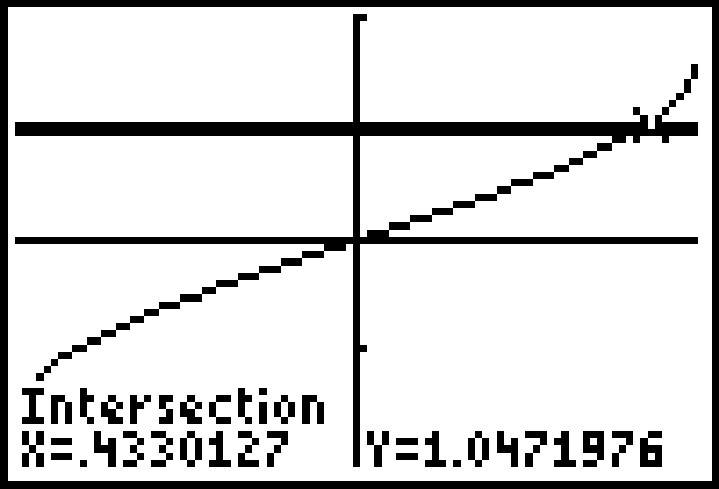
\includegraphics[width=2in]{./IntroTrigGraphics/ARCSINEQN.jpg} &

\hspace{1in} 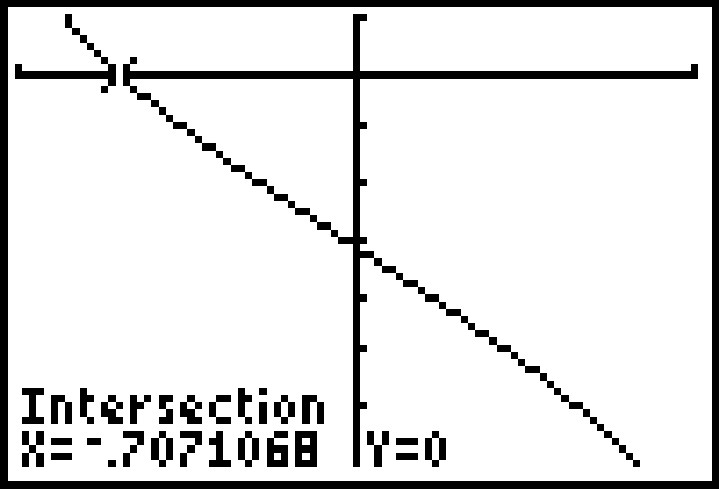
\includegraphics[width=2in]{./IntroTrigGraphics/ARCCOSEQN.jpg} \\

$y = \arcsin(2x)$ and \boldmath $y = \frac{\pi}{3}$     & 

 \hspace{1in}  $y=4\arccos(x) - 3\pi$ \\

\end{tabular}

\end{center}


\item From $3 \, \text{arcsec}(2x-1) + \pi = 2 \pi$, we get $\text{arcsec}(2x-1) = \frac{\pi}{3}$.  As we saw in Section \ref{ArcTrig}, there are two possible ranges for the arcsecant function.  Fortunately, both ranges contain $\frac{\pi}{3}$.  Applying Theorem \ref{arcsecantcosecantfunctionprops1} / \ref{arcsecantcosecantfunctionprops2}, we get

\[ \begin{array}{rclr}

\text{arcsec}(2x-1)& = & \frac{\pi}{3} & \\ [5pt]
\sec(\text{arcsec}(2x-1)) & = & \sec\left(\frac{\pi}{3}\right) & \\ [5pt]
2x -1 & = & 2 & \text{Since $\sec(\text{arcsec}(u)) = u$} \\ [5pt]
    x & = & \frac{3}{2} \\ \end{array} \]



To check using our calculator, we need to graph $y=3 \, \text{arcsec}(2x-1) + \pi$.  To do so, we make use of the identity $\text{arcsec}(u) = \arccos\left(\frac{1}{u}\right)$ from Theorems \ref{arcsecantcosecantfunctionprops1} and \ref{arcsecantcosecantfunctionprops2}.\footnote{Since we are checking for solutions where arcsecant is positive, we know $u = 2x-1 \geq 1$, and so the identity applies in both cases.} We see the graph of $y=3 \arccos\left(\frac{1}{2x-1}\right) + \pi$ and the horizontal line $y = 2\pi$ intersect at $\frac{3}{2} = 1.5$.

\item  With the presence of both $\arctan^{2}(x)$ ( $= (\arctan(x))^2$) and $\arctan(x)$, we substitute $u = \arctan(x)$.  The equation  $4\arctan^2(x)-3\pi \arctan(x)-\pi^2 = 0$ becomes $4u^2 -3\pi u - \pi^2 = 0$.  Factoring,\footnote{It's not as bad as it looks...  don't let the $\pi$ throw you!} we get $(4u+\pi)(u - \pi) = 0$, so $u = \arctan(x) = -\frac{\pi}{4}$ or $u = \arctan(x) = \pi$.  Since $-\frac{\pi}{4}$ is in the range of arctangent, but $\pi$ is not, we only get solutions from the first equation.  Using Theorem \ref{arctangentcotangentfunctionprops}, we get

\[ \begin{array}{rclr}

\arctan(x) & = & -\frac{\pi}{4} & \\ [5pt]
\tan(\arctan(x)) & = & \tan\left(-\frac{\pi}{4}\right) & \\ [5pt]
x & = & -1 & \text{Since $\tan(\arctan(u)) = u$.} \\ \end{array}\]

The calculator verifies our result.

\begin{center}

\begin{tabular}{cc}

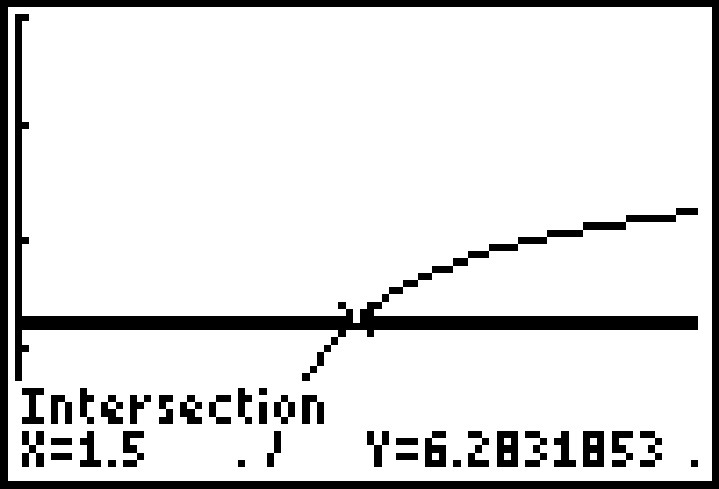
\includegraphics[width=2in]{./IntroTrigGraphics/ARCSECEQN.jpg} &

\hspace{1in} 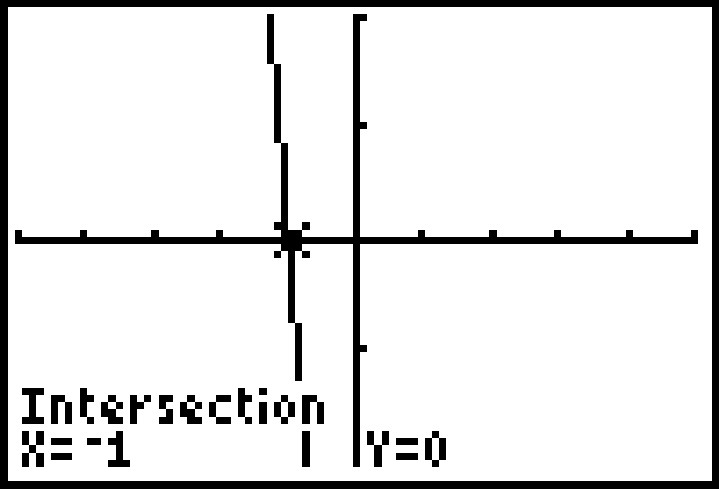
\includegraphics[width=2in]{./IntroTrigGraphics/ARCTANEQN.jpg} \\

$y = 3 \, \text{arcsec}(2x-1) + \pi$ and \boldmath $y = 2\pi$     & 

 \hspace{1in}  $y=4\arctan^2(x)-3\pi \arctan(x)-\pi^2$ \\

\end{tabular}

\end{center}

\item Since the inverse trigonometric functions are continuous on their domains, we can solve inequalities featuring these functions using sign diagrams. Since all of the nonzero terms of  $\pi^2-4\arccos^{2}(x) < 0$ are on one side of the inequality, we let $f(x) = \pi^2-4\arccos^{2}(x)$ and note the domain of $f$ is limited by the $\arccos(x)$ to $[-1,1]$.  Next, we find the zeros of $f$ by setting $f(x) = \pi^2-4\arccos^{2}(x) = 0$.  We get $\arccos(x) = \pm \frac{\pi}{2}$, and since the range of arccosine is $[0,\pi]$, we focus our attention on $\arccos(x) = \frac{\pi}{2}$.  Using Theorem \ref{arccosinesinefunctionprops}, we get $x = \cos\left(\frac{\pi}{2}\right) = 0$ as our only zero.  Hence, we have two test intervals, $[-1,0)$ and $(0,1]$.  Choosing test values $x = \pm 1$, we get $f(-1) = -3\pi^2 < 0$ and $f(1) = \pi^2 > 0$.  Since we are looking for where $f(x) = \pi^2-4\arccos^{2}(x) < 0$, our answer is $[-1,0)$.  The calculator confirms that for these values of $x$, the graph of $y = \pi^2-4\arccos^{2}(x)$ is below $y = 0$ (the $x$-axis.)


\begin{center}

\begin{tabular}{m{2in}c}

\begin{mfpic}[10]{-5}{5}{-2}{2}
\polyline{(-5,0),(5,0)}
\xmarks{-5,0,5}
\tiny
\tlpointsep{6pt}
\normalsize
\tlabel[cc](-5,-1){$-1$}
\tlabel[cc](-2.5,1){$(-)$}
\tlabel[cc](0,1){$0$}
\tlabel[cc](0,-1){$0$}
\tlabel[cc](5,-1){$1$}
\tlabel[cc](2.5,1){$(+)$}
\end{mfpic} 
& 

\hspace{.75in} 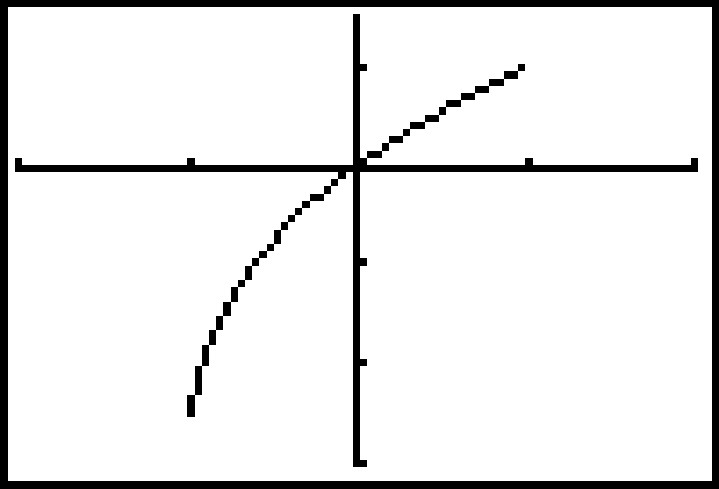
\includegraphics[width=2in]{./IntroTrigGraphics/ARCCOSINEQ.jpg} \\

& \hspace{.75in} $y = \pi^2-4\arccos^{2}(x)$  \\

\end{tabular}

\end{center}



\item   To begin, we rewrite $4 \, \text{arccot}(3x) > \pi$ as $4 \, \text{arccot}(3x) -  \pi > 0$.  We let $f(x) = 4 \, \text{arccot}(3x) -  \pi$, and note the domain of $f$ is all real numbers, $(-\infty, \infty)$.  To find the zeros of $f$, we set $f(x) = 4 \, \text{arccot}(3x) -  \pi = 0$ and solve.  We get $\text{arccot}(3x) = \frac{\pi}{4}$, and since $\frac{\pi}{4}$ is in the range of arccotangent, we may apply Theorem \ref{arctangentcotangentfunctionprops} and solve 

\[ \begin{array}{rclr}

\text{arccot}(3x) & = & \frac{\pi}{4} & \\ [5pt]
\cot(\text{arccot}(3x)) & = & \cot\left(\frac{\pi}{4}\right) & \\ [5pt]
3x & = & 1 & \text{Since $\cot(\text{arccot}(u)) = u$.} \\ [5pt]
x & = & \frac{1}{3} &  \\ \end{array}\]


Next, we make a sign diagram for $f$.  Since the domain of $f$ is all real numbers, and there is only one zero of $f$, $x = \frac{1}{3}$, we have two test intervals, $\left(-\infty, \frac{1}{3}\right)$ and  $\left(\frac{1}{3}, \infty \right)$. Ideally, we wish to find test values $x$ in these intervals so that $\text{arccot}(4x)$ corresponds to one of our oft-used `common' angles.  After a bit of computation,\footnote{Set $3x$ equal to the cotangents of the `common angles' and choose accordingly.} we choose $x=0$ for $x < \frac{1}{3}$ and for $x > \frac{1}{3}$, we choose $x = \frac{\sqrt{3}}{3}$.  We find $f(0) = \pi > 0$ and $f\left(\frac{\sqrt{3}}{3}\right) = -\frac{\pi}{3} < 0$.  Since we are looking for where $f(x) = 4 \, \text{arccot}(3x) -  \pi > 0$, we get our answer $\left(-\infty, \frac{1}{3}\right)$.  To check graphically, we use the technique in number \ref{arccotangentcalc} of Example \ref{arcstuffoncalc} in Section \ref{ArcTrig} to graph $y = 4 \, \text{arccot}(3x)$  and we see it is above the horizontal line $y = \pi$ on $\left(-\infty, \frac{1}{3}\right) = \left(-\infty, 0.\overline{3}\right)$.



\begin{center}

\begin{tabular}{m{2in}c}

\begin{mfpic}[10]{-5}{5}{-2}{2}
\arrow \reverse \arrow \polyline{(-5,0),(5,0)}
\xmarks{0}
\tiny
\tlpointsep{6pt}
\normalsize

\tlabel[cc](-2.5,1){$(+)$}
\tlabel[cc](0,1){$0$}
\tlabel[cc](0,-1){$\frac{1}{3}$}
\tlabel[cc](2.5,1){$(-)$}
\end{mfpic} & 

\hspace{.75in} 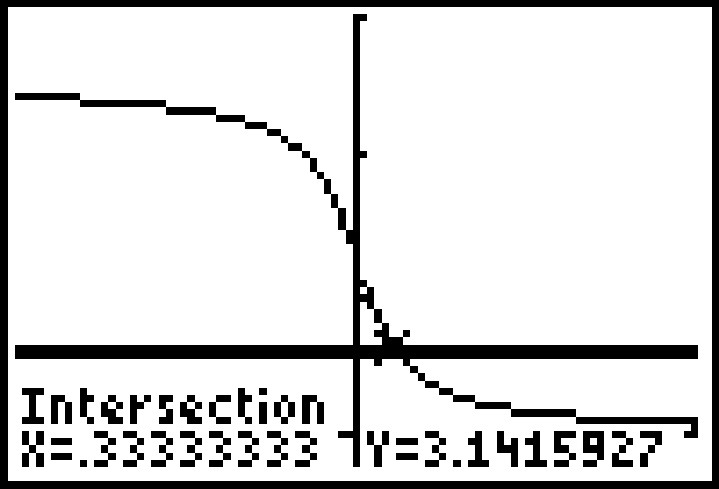
\includegraphics[width=2in]{./IntroTrigGraphics/ARCCOTINEQ.jpg} \\

& \hspace{.75in} $y = 4 \, \text{arccot}(3x)$ and \boldmath $y=\pi$  \\

\end{tabular}

\end{center}


\end{enumerate}

\vspace{-.25in} \qed

\end{ex}
 

 
\newpage 
 
\newpage

\subsection{Exercises}


In Exercises \ref{solvebasicfirst} - \ref{solvebasiclast}, find \underline{all} of the exact solutions of the  equation and then list those solutions which are in the interval $[0, 2\pi)$.

\begin{multicols}{3}

\begin{enumerate}

\item $\sin \left( 5x \right) = 0$ \vphantom{$\dfrac{\sqrt{3}}{2}$} \label{solvebasicfirst}
\item $\cos \left( 3x \right) = \dfrac{1}{2}$ \vphantom{$\dfrac{\sqrt{3}}{2}$}
\item $\sin \left( -2x \right) = \dfrac{\sqrt{3}}{2}$ 

\setcounter{HW}{\value{enumi}}

\end{enumerate}

\end{multicols}

\begin{multicols}{3}

\begin{enumerate}

\setcounter{enumi}{\value{HW}}

\item $\tan \left( 6x \right) = 1$
\item $\csc \left( 4x \right) = -1$
\item $\sec \left( 3x \right) = \sqrt{2}$

\setcounter{HW}{\value{enumi}}

\end{enumerate}

\end{multicols}

\begin{multicols}{3}

\begin{enumerate}

\setcounter{enumi}{\value{HW}}

\item $\cot \left( 2x \right) = -\dfrac{\sqrt{3}}{3}$
\item $\cos \left( 9x \right) = 9$ \vphantom{$\dfrac{\sqrt{3}}{2}$}
\item $\sin \left( \dfrac{x}{3} \right) = \dfrac{\sqrt{2}}{2}$

\setcounter{HW}{\value{enumi}}

\end{enumerate}

\end{multicols}

\begin{multicols}{3}

\begin{enumerate}

\setcounter{enumi}{\value{HW}}

\item $\cos \left( x + \dfrac{5\pi}{6} \right) = 0$
\item $\sin \left( 2x - \dfrac{\pi}{3} \right) = -\dfrac{1}{2}$
\item $2\cos \left( x + \dfrac{7\pi}{4} \right) = \sqrt{3}$

\setcounter{HW}{\value{enumi}}

\end{enumerate}

\end{multicols}

\begin{multicols}{3}

\begin{enumerate}

\setcounter{enumi}{\value{HW}}

\item $\csc(x) = 0$
\item $\tan \left( 2x - \pi \right) = 1$
\item $\tan^{2} \left( x \right) = 3$

\setcounter{HW}{\value{enumi}}

\end{enumerate}

\end{multicols}

\begin{multicols}{3}

\begin{enumerate}

\setcounter{enumi}{\value{HW}}

\item $\sec^{2} \left( x \right) = \dfrac{4}{3}$
\item $\cos^{2} \left( x \right) = \dfrac{1}{2}$
\item $\sin^{2} \left( x \right) = \dfrac{3}{4}$ \label{solvebasiclast}

\setcounter{HW}{\value{enumi}}

\end{enumerate}

\end{multicols}

In Exercises \ref{solveidentfirst} - \ref{solveidentlast}, solve the equation, giving the exact solutions which lie in $[0, 2\pi)$


\begin{multicols}{2}

\begin{enumerate}

\setcounter{enumi}{\value{HW}}

\item $\sin \left( x \right) = \cos \left( x \right)$ \label{solveidentfirst}
\item $\sin \left( 2x \right) = \sin \left( x \right)$

\setcounter{HW}{\value{enumi}}

\end{enumerate}

\end{multicols}

\begin{multicols}{2}

\begin{enumerate}

\setcounter{enumi}{\value{HW}}

\item $\sin \left( 2x \right) = \cos \left( x \right)$
\item $\cos \left( 2x \right) = \sin \left( x \right)$

\setcounter{HW}{\value{enumi}}

\end{enumerate}

\end{multicols}

\begin{multicols}{2}

\begin{enumerate}

\setcounter{enumi}{\value{HW}}

\item $\cos \left( 2x \right) = \cos \left( x \right)$
\item  $\cos(2x) = 2 - 5\cos(x)$

\setcounter{HW}{\value{enumi}}

\end{enumerate}

\end{multicols}

\begin{multicols}{2}

\begin{enumerate}

\setcounter{enumi}{\value{HW}}

\item  $3\cos(2x) + \cos(x) + 2 = 0$
\item  $\cos(2x) = 5\sin(x) - 2$

\setcounter{HW}{\value{enumi}}

\end{enumerate}

\end{multicols}

\begin{multicols}{2}

\begin{enumerate}

\setcounter{enumi}{\value{HW}}

\item  $3\cos(2x) = \sin(x) + 2$
\item  $2\sec^{2}(x) = 3 - \tan(x)$

\setcounter{HW}{\value{enumi}}

\end{enumerate}

\end{multicols}

\begin{multicols}{2}

\begin{enumerate}

\setcounter{enumi}{\value{HW}}

\item  $\tan^{2}(x) = 1-\sec(x)$
\item  $\cot^{2}(x) = 3\csc(x) - 3$

\setcounter{HW}{\value{enumi}}

\end{enumerate}

\end{multicols}

\begin{multicols}{2}

\begin{enumerate}

\setcounter{enumi}{\value{HW}}

\item  $\sec(x) = 2\csc(x)$
\item  $\cos(x)\csc(x)\cot(x) = 6-\cot^{2}(x)$

\setcounter{HW}{\value{enumi}}

\end{enumerate}

\end{multicols}

\begin{multicols}{2}

\begin{enumerate}

\setcounter{enumi}{\value{HW}}

\item  $\sin(2x) = \tan(x)$
\item  $\cot^{4}(x) = 4\csc^{2}(x) - 7$

\setcounter{HW}{\value{enumi}}

\end{enumerate}

\end{multicols}

\begin{multicols}{2}

\begin{enumerate}

\setcounter{enumi}{\value{HW}}

\item  $\cos(2x) + \csc^{2}(x) = 0$
\item $\tan^{3} \left( x \right) = 3\tan \left( x \right)$

\setcounter{HW}{\value{enumi}}

\end{enumerate}

\end{multicols}

\begin{multicols}{2}

\begin{enumerate}

\setcounter{enumi}{\value{HW}}

\item $\tan^{2} \left( x \right) = \dfrac{3}{2} \sec \left( x \right)$
\item $\cos^{3} \left( x \right) = -\cos \left( x \right)$ \vphantom{$\dfrac{3}{2}$}

\setcounter{HW}{\value{enumi}}

\end{enumerate}

\end{multicols}

\begin{multicols}{2}

\begin{enumerate}

\setcounter{enumi}{\value{HW}}

\item $\tan (2x) - 2\cos(x) = 0$
\item $\csc^{3}(x) + \csc^{2}(x) = 4\csc(x) + 4$

\setcounter{HW}{\value{enumi}}

\end{enumerate}

\end{multicols}
\enlargethispage{.5in}
\vspace{-.1in}
\begin{multicols}{2}

\begin{enumerate}

\setcounter{enumi}{\value{HW}}

\item $2\tan(x) = 1 - \tan^{2}(x)$
\item $\tan \left( x \right) = \sec \left( x \right)$ \label{solveidentlast}

\setcounter{HW}{\value{enumi}}

\end{enumerate}

\end{multicols}

In Exercises \ref{solvemoreidentfirst} - \ref{solvemoreidentlast}, solve the equation, giving the exact solutions which lie in $[0, 2\pi)$


\begin{multicols}{2}

\begin{enumerate}

\setcounter{enumi}{\value{HW}}

\item $\sin(6x) \cos(x) = -\cos(6x) \sin(x)$ \label{solvemoreidentfirst}
\item  $\sin(3x)\cos(x) = \cos(3x) \sin(x)$

\setcounter{HW}{\value{enumi}}

\end{enumerate}

\end{multicols}

\begin{multicols}{2}

\begin{enumerate}

\setcounter{enumi}{\value{HW}}

\item $\cos(2x)\cos(x) + \sin(2x)\sin(x) = 1$ \vphantom{$\dfrac{\sqrt{3}}{2}$}
\item \small $\cos(5x)\cos(3x) - \sin(5x)\sin(3x) = \dfrac{\sqrt{3}}{2}$ \normalsize

\setcounter{HW}{\value{enumi}}

\end{enumerate}

\end{multicols}

\begin{multicols}{2}

\begin{enumerate}

\setcounter{enumi}{\value{HW}}

%Sinusoids
\item $\sin(x) + \cos(x) = 1$
\item  $\sin(x) + \sqrt{3} \cos(x) = 1$

\setcounter{HW}{\value{enumi}}

\end{enumerate}

\end{multicols}

\begin{multicols}{2}

\begin{enumerate}

\setcounter{enumi}{\value{HW}}

\item  $\sqrt{2} \cos(x) - \sqrt{2} \sin(x) = 1$
\item  $\sqrt{3} \sin(2x) +  \cos(2x) = 1$

\setcounter{HW}{\value{enumi}}

\end{enumerate}

\end{multicols}

\begin{multicols}{2}

\begin{enumerate}

\setcounter{enumi}{\value{HW}}

\item $\cos(2x) - \sqrt{3} \sin(2x) = \sqrt{2}$
\item $3\sqrt{3}\sin(3x) - 3\cos(3x) = 3\sqrt{3}$

\setcounter{HW}{\value{enumi}}

\end{enumerate}

\end{multicols}

\begin{multicols}{2}

\begin{enumerate}

\setcounter{enumi}{\value{HW}}

\item  $\cos(3x) = \cos(5x)$
\item $\cos(4x) = \cos(2x)$

\setcounter{HW}{\value{enumi}}

\end{enumerate}

\end{multicols}

\begin{multicols}{2}

\begin{enumerate}

\setcounter{enumi}{\value{HW}}

\item $\sin(5x) = \sin(3x)$
\item $\cos(5x) = -\cos(2x)$

\setcounter{HW}{\value{enumi}}

\end{enumerate}

\end{multicols}

\begin{multicols}{2}
\begin{enumerate}
\setcounter{enumi}{\value{HW}}

\item $\sin(6x) + \sin(x) = 0$
\item $\tan(x) = \cos(x)$ \label{solvemoreidentlast}

\setcounter{HW}{\value{enumi}}
\end{enumerate}
\end{multicols}

In Exercises \ref{firstinveqn} - \ref{lastinveqn}, solve the equation.

\begin{multicols}{2}
\begin{enumerate}
\setcounter{enumi}{\value{HW}}

\item $\arccos(2x) = \pi$  \label{firstinveqn}  %Ans $x = -\frac{1}{2}$
\item $\pi - 2\arcsin(x) = 2\pi$   %Ans  $x=-1$

\setcounter{HW}{\value{enumi}}
\end{enumerate}
\end{multicols}

\begin{multicols}{2}
\begin{enumerate}
\setcounter{enumi}{\value{HW}}

\item $4\arctan(3x-1)-\pi=0$   %Ans $x = \frac{2}{3}$
\item $6 \, \text{arccot}(2x) - 5\pi = 0$   %Ans  $x=-\frac{\sqrt{3}}{2}$

\setcounter{HW}{\value{enumi}}
\end{enumerate}
\end{multicols}


\begin{multicols}{2}
\begin{enumerate}
\setcounter{enumi}{\value{HW}}

\item $4 \,\text{arcsec}\left(\frac{x}{2}\right) = \pi$   %Ans $x = 2\sqrt{2}$
\item $12 \,\text{arccsc}\left(\frac{x}{3}\right) = 2\pi$   %Ans $x = 6$

\setcounter{HW}{\value{enumi}}
\end{enumerate}
\end{multicols}

\begin{multicols}{2}
\begin{enumerate}
\setcounter{enumi}{\value{HW}}

\item $9 \arcsin^{2}(x) - \pi^2 = 0$   %Ans $x = \pm \frac{\sqrt{3}}{2}$
\item $9 \arccos^{2}(x) - \pi^2 = 0$   %Ans $x = \frac{1}{2}$

\setcounter{HW}{\value{enumi}}
\end{enumerate}
\end{multicols}

\begin{multicols}{2}
\begin{enumerate}
\setcounter{enumi}{\value{HW}}

\item $8 \, \text{arccot}^{2}(x)+3\pi^2=10 \pi \, \text{arccot}(x)$   %Ans $x = -1,0$
\item $6 \arctan(x)^2= \pi \arctan(x)+\pi^2$  \label{lastinveqn}  %Ans $x = -\sqrt{3}$

\setcounter{HW}{\value{enumi}}
\end{enumerate}
\end{multicols}


In Exercises \ref{firstineqfirst} - \ref{firstineqlast}, solve the inequality.  Express the exact answer in \underline{interval} notation, restricting your attention to $0 \leq x \leq 2\pi$.

\begin{multicols}{3}

\begin{enumerate}

\setcounter{enumi}{\value{HW}}

\item $\sin \left( x \right) \leq 0$ \label{firstineqfirst}
\item $\tan \left( x \right) \geq \sqrt{3}$
\item $\sec^{2} \left( x \right) \leq 4$

\setcounter{HW}{\value{enumi}}

\end{enumerate}

\end{multicols}

\begin{multicols}{3}

\begin{enumerate}

\setcounter{enumi}{\value{HW}}

\item $\cos^{2} \left( x \right) > \dfrac{1}{2}$
\item $\cos \left( 2x \right) \leq 0$ \vphantom{$\dfrac{1}{2}$}
\item $\sin \left( x + \dfrac{\pi}{3} \right) > \dfrac{1}{2}$

\setcounter{HW}{\value{enumi}}

\end{enumerate}

\end{multicols}

\begin{multicols}{3}

\begin{enumerate}

\setcounter{enumi}{\value{HW}}

\item $\cot^{2} \left( x \right) \geq \dfrac{1}{3}$
\item $2\cos(x) \geq 1$ \vphantom{$\dfrac{1}{2}$}
\item $\sin(5x) \geq 5$ \vphantom{$\dfrac{1}{2}$}

\setcounter{HW}{\value{enumi}}

\end{enumerate}

\end{multicols}

\begin{multicols}{3}

\begin{enumerate}

\setcounter{enumi}{\value{HW}}

\item $\cos(3x) \leq 1$
\item $\sec(x) \leq \sqrt{2}$
\item $\cot(x) \leq 4$ \label{firstineqlast}

\setcounter{HW}{\value{enumi}}
\end{enumerate}
\end{multicols}

\pagebreak

In Exercises \ref{secondineqefirst} - \ref{secondineqlast}, solve the inequality.  Express the exact answer in \underline{interval} notation, restricting your attention to $-\pi \leq x \leq \pi$.

\begin{multicols}{3}

\begin{enumerate}

\setcounter{enumi}{\value{HW}}

\item $\cos \left( x \right) > \dfrac{\sqrt{3}}{2}$ \label{secondineqefirst}
\item  $\sin(x) > \dfrac{1}{3}$ \vphantom{$\dfrac{\sqrt{3}}{2}$}
\item $\sec \left( x \right) \leq 2$ \vphantom{$\dfrac{\sqrt{3}}{2}$}

\setcounter{HW}{\value{enumi}}

\end{enumerate}

\end{multicols}

\begin{multicols}{3}

\begin{enumerate}

\setcounter{enumi}{\value{HW}}

\item $\sin^{2} \left( x \right) < \dfrac{3}{4}$
\item $\cot \left( x \right) \geq -1$ \vphantom{$\dfrac{1}{2}$}
\item $\cos(x) \geq \sin(x)$ \vphantom{$\dfrac{1}{2}$} \label{secondineqlast}

\setcounter{HW}{\value{enumi}}

\end{enumerate}

\end{multicols}

%\pagebreak

In Exercises \ref{thirdineqfirst} - \ref{thirdineqlast}, solve the inequality.  Express the exact answer in \underline{interval} notation, restricting your attention to $-2\pi \leq x \leq 2\pi$.

\begin{multicols}{3}

\begin{enumerate}

\setcounter{enumi}{\value{HW}}

\item $\csc \left( x \right) > 1$ \vphantom{$\dfrac{1}{2}$} \label{thirdineqfirst}
\item  $\cos(x) \leq \dfrac{5}{3}$
\item  $\cot(x) \geq 5$ \vphantom{$\dfrac{1}{2}$}

\setcounter{HW}{\value{enumi}}

\end{enumerate}

\end{multicols}

\begin{multicols}{3}

\begin{enumerate}

\setcounter{enumi}{\value{HW}}

\item $\tan^{2} \left( x \right) \geq 1$
\item $\sin(2x) \geq \sin(x)$
\item $\cos(2x) \leq \sin(x)$ \label{thirdineqlast}

\setcounter{HW}{\value{enumi}}

\end{enumerate}

\end{multicols}

In Exercises \ref{invineqfirst} - \ref{invineqlast}, solve the given inequality.

\begin{multicols}{4}

\begin{enumerate}

\setcounter{enumi}{\value{HW}}

\item $\arcsin(2x) > 0$ \label{invineqfirst}  
\item $3 \arccos(x) \leq \pi$
\item $6 \, \text{arccot}(7x) \geq \pi$  
\item $\pi > 2\arctan(x)$ 

\setcounter{HW}{\value{enumi}}

\end{enumerate}

\end{multicols}

\begin{multicols}{2}

\begin{enumerate}

\setcounter{enumi}{\value{HW}}

\item $2\arcsin(x)^2 > \pi \arcsin(x)$  
\item $12 \arccos(x)^2+2\pi^2>11\pi \arccos(x)$ \label{invineqlast} 

\setcounter{HW}{\value{enumi}}

\end{enumerate}

\end{multicols}

In Exercises \ref{domainfirst} - \ref{domainlast}, express the domain of the function using the extended interval notation. (See page \pageref{extendedinterval} in Section \ref{circularfunctionsbeyond} for details.)

\begin{multicols}{3}

\begin{enumerate}

\setcounter{enumi}{\value{HW}}

\item $f(x) = \dfrac{1}{\cos(x) - 1}$ \vphantom{$\dfrac{\cos(x)}{\sin(x) + 1}$} \label{domainfirst}
\item $f(x) = \dfrac{\cos(x)}{\sin(x) + 1}$
\item $f(x) = \sqrt{\tan^{2}(x) - 1}$ \vphantom{$\dfrac{\cos(x)}{\sin(x) + 1}$}

\setcounter{HW}{\value{enumi}}

\end{enumerate}

\end{multicols}

\begin{multicols}{3}

\begin{enumerate}

\setcounter{enumi}{\value{HW}}

\item $f(x) = \sqrt{2 - \sec(x)}$ \vphantom{$\dfrac{\cos(x)}{\sin(x) + 1}$}
\item $f(x) = \csc(2x)$ \vphantom{$\dfrac{\cos(x)}{\sin(x) + 1}$}
\item $f(x) = \dfrac{\sin(x)}{2 + \cos(x)}$

\setcounter{HW}{\value{enumi}}

\end{enumerate}

\end{multicols}

\begin{multicols}{3}

\begin{enumerate}

\setcounter{enumi}{\value{HW}}

\item $f(x) = 3\csc(x) + 4\sec(x)$ 
\item $f(x) = \ln\left( |\cos(x)| \right)$
\item $f(x) = \arcsin(\tan(x))$ \label{domainlast}

\setcounter{HW}{\value{enumi}}

\end{enumerate}

\end{multicols}

\begin{enumerate}

\setcounter{enumi}{\value{HW}}

\item With the help of your classmates, determine the number of solutions to $\sin(x) = \frac{1}{2}$ in $[0,2\pi)$.  Then find the number of solutions to $\sin(2x) = \frac{1}{2}$,  $\sin(3x) = \frac{1}{2}$ and $\sin(4x) = \frac{1}{2}$ in $[0,2\pi)$.  A pattern should emerge.  Explain how this pattern would help you solve equations like $\sin(11x) = \frac{1}{2}$.  Now consider $\sin\left(\frac{x}{2}\right)  = \frac{1}{2}$,  $\sin\left(\frac{3x}{2}\right)  = \frac{1}{2}$ and $\sin\left(\frac{5x}{2}\right)  = \frac{1}{2}$.  What do you find?  Replace $\dfrac{1}{2}$ with $-1$ and repeat the whole exploration.

\end{enumerate}


\newpage

\subsection{Answers}

\begin{enumerate}

\item $x = \dfrac{\pi k}{5}; \; x = 0, \dfrac{\pi}{5}, \dfrac{2\pi}{5}, \dfrac{3\pi}{5}, \dfrac{4\pi}{5}, \pi, \dfrac{6\pi}{5}, \dfrac{7\pi}{5}, \dfrac{8\pi}{5}, \dfrac{9\pi}{5}$

\item $x = \dfrac{\pi}{9} + \dfrac{2\pi k}{3}$ or $x = \dfrac{5\pi}{9} + \dfrac{2\pi k}{3}; \; x = \dfrac{\pi}{9}, \dfrac{5\pi}{9}, \dfrac{7\pi}{9}, \dfrac{11\pi}{9}, \dfrac{13\pi}{9}, \dfrac{17\pi}{9}$

\item $x = \dfrac{2\pi}{3} + \pi k$ or $x = \dfrac{5\pi}{6} + \pi k; \; x = \dfrac{2\pi}{3}, \dfrac{5\pi}{6}, \dfrac{5\pi}{3}, \dfrac{11\pi}{6}$

\item $x = \dfrac{\pi}{24} + \dfrac{\pi k}{6}; \; x = \dfrac{\pi}{24}, \dfrac{5\pi}{24}, \dfrac{3\pi}{8}, \dfrac{13\pi}{24}, \dfrac{17\pi}{24}, \dfrac{7\pi}{8}, \dfrac{25\pi}{24}, \dfrac{29\pi}{24}, \dfrac{11\pi}{8}, \dfrac{37\pi}{24}, \dfrac{41\pi}{24}, \dfrac{15\pi}{8}$

\item $x = \dfrac{3\pi}{8} + \dfrac{\pi k}{2}; \; x = \dfrac{3\pi}{8}, \dfrac{7\pi}{8}, \dfrac{11\pi}{8}, \dfrac{15\pi}{8}$

\item $x = \dfrac{\pi}{12} + \dfrac{2\pi k}{3}$ or $x = \dfrac{7\pi}{12} + \dfrac{2\pi k}{3}; \; x = \dfrac{\pi}{12}, \dfrac{7\pi}{12}, \dfrac{3\pi}{4}, \dfrac{5\pi}{4}, \dfrac{17\pi}{12}, \dfrac{23\pi}{12}$

\item $x = \dfrac{\pi}{3} + \dfrac{\pi k}{2}; \; x = \dfrac{\pi}{3}, \dfrac{5\pi}{6}, \dfrac{4\pi}{3}, \dfrac{11\pi}{6}$

\item No solution

\item $x = \dfrac{3\pi}{4} + 6\pi k$ or $x = \dfrac{9\pi}{4} + 6\pi k; \; x = \dfrac{3\pi}{4}$

\item $x = -\dfrac{\pi}{3} + \pi k; \; x = \dfrac{2\pi}{3}, \dfrac{5\pi}{3}$

\item $x = \dfrac{3\pi}{4} + \pi k$ or $x = \dfrac{13\pi}{12} + \pi k; \; x = \dfrac{\pi}{12}, \dfrac{3\pi}{4}, \dfrac{13\pi}{12}, \dfrac{7\pi}{4}$

\item $x = -\dfrac{19\pi}{12} + 2\pi k$ or $x = \dfrac{\pi}{12} + 2\pi k; \; x = \dfrac{\pi}{12}, \dfrac{5\pi}{12}$

\item No solution

\item $x = \dfrac{5\pi}{8} + \dfrac{\pi k}{2}; \; x = \dfrac{\pi}{8}, \dfrac{5\pi}{8}, \dfrac{9\pi}{8}, \dfrac{13\pi}{8}$

\item $x = \dfrac{\pi}{3} + \pi k$ or $x = \dfrac{2\pi}{3} + \pi k; \; x = \dfrac{\pi}{3}, \dfrac{2\pi}{3}, \dfrac{4\pi}{3}, \dfrac{5\pi}{3}$

\item $x = \dfrac{\pi}{6} + \pi k$ or $x = \dfrac{5\pi}{6} + \pi k; \; x = \dfrac{\pi}{6}, \dfrac{5\pi}{6}, \dfrac{7\pi}{6}, \dfrac{11\pi}{6}$

\item $x = \dfrac{\pi}{4} + \dfrac{\pi k}{2}; \; x = \dfrac{\pi}{4}, \dfrac{3\pi}{4}, \dfrac{5\pi}{4}, \dfrac{7\pi}{4}$

\item $x = \dfrac{\pi}{3} + \pi k$ or $x = \dfrac{2\pi}{3} + \pi k; \; x = \dfrac{\pi}{3}, \dfrac{2\pi}{3}, \dfrac{4\pi}{3}, \dfrac{5\pi}{3}$

\setcounter{HW}{\value{enumi}}

\end{enumerate}

\begin{multicols}{2}

\begin{enumerate}

\setcounter{enumi}{\value{HW}}

\item $x = \dfrac{\pi}{4}, \dfrac{5\pi}{4}$
\item $x = 0, \dfrac{\pi}{3}, \pi, \dfrac{5\pi}{3}$

\setcounter{HW}{\value{enumi}}

\end{enumerate}

\end{multicols}

\begin{multicols}{2}

\begin{enumerate}

\setcounter{enumi}{\value{HW}}

\item $x = \dfrac{\pi}{6}, \dfrac{\pi}{2}, \dfrac{5\pi}{6}, \dfrac{3\pi}{2}$
\item $x = \dfrac{\pi}{6}, \dfrac{5\pi}{6}, \dfrac{3\pi}{2}$

\setcounter{HW}{\value{enumi}}

\end{enumerate}

\end{multicols}

\begin{multicols}{2}

\begin{enumerate}

\setcounter{enumi}{\value{HW}}

\item $x = 0, \dfrac{2\pi}{3}, \dfrac{4\pi}{3}$
\item  $x=\dfrac{\pi}{3}, \dfrac{5\pi}{3}$

\setcounter{HW}{\value{enumi}}

\end{enumerate}

\end{multicols}

\begin{multicols}{2}

\begin{enumerate}

\setcounter{enumi}{\value{HW}}

\item  $x = \dfrac{2\pi}{3}, \dfrac{4\pi}{3}, \arccos\left(\dfrac{1}{3}\right), 2\pi -\arccos\left(\dfrac{1}{3}\right) $
\item  $x=\dfrac{\pi}{6}, \dfrac{5\pi}{6}$

\setcounter{HW}{\value{enumi}}

\end{enumerate}

\end{multicols}

\begin{multicols}{2}

\begin{enumerate}

\setcounter{enumi}{\value{HW}}

\item  $x = \dfrac{7\pi}{6}, \dfrac{11\pi}{6}, \arcsin\left(\dfrac{1}{3}\right), \pi - \arcsin\left(\dfrac{1}{3}\right) $
\item  $x=\dfrac{3\pi}{4}, \dfrac{7\pi}{4}, \arctan\left(\dfrac{1}{2}\right), \pi +\arctan\left(\dfrac{1}{2}\right) $

\setcounter{HW}{\value{enumi}}

\end{enumerate}

\end{multicols}

\begin{multicols}{2}

\begin{enumerate}

\setcounter{enumi}{\value{HW}}

\item  $x=0, \dfrac{2\pi}{3}, \dfrac{4\pi}{3}$
\item  $x=\dfrac{\pi}{6}, \dfrac{5\pi}{6}, \dfrac{\pi}{2}$

\setcounter{HW}{\value{enumi}}

\end{enumerate}

\end{multicols}

\begin{multicols}{2}

\begin{enumerate}

\setcounter{enumi}{\value{HW}}

\item  $x=\arctan(2), \pi + \arctan(2)$ \vphantom{$\dfrac{7\pi}{6}$}
\item  $x = \dfrac{\pi}{6}, \dfrac{7\pi}{6}, \dfrac{5\pi}{6}, \dfrac{11\pi}{6}$

\setcounter{HW}{\value{enumi}}

\end{enumerate}

\end{multicols}

\begin{multicols}{2}

\begin{enumerate}

\setcounter{enumi}{\value{HW}}

\item  $x = 0, \pi, \dfrac{\pi}{4}, \dfrac{3\pi}{4}, \dfrac{5\pi}{4}, \dfrac{7\pi}{4}$
\item  $x = \dfrac{\pi}{6}, \dfrac{\pi}{4}, \dfrac{3\pi}{4}, \dfrac{5\pi}{6}, \dfrac{7\pi}{6}, \dfrac{5\pi}{4}, \dfrac{7\pi}{4}, \dfrac{11\pi}{6}$

\setcounter{HW}{\value{enumi}}

\end{enumerate}

\end{multicols}

\begin{multicols}{2}

\begin{enumerate}

\setcounter{enumi}{\value{HW}}

\item  $x = \dfrac{\pi}{2}, \dfrac{3\pi}{2}$
\item $x = 0, \dfrac{\pi}{3}, \dfrac{2\pi}{3}, \pi, \dfrac{4\pi}{3}, \dfrac{5\pi}{3}$

\setcounter{HW}{\value{enumi}}

\end{enumerate}

\end{multicols}

\begin{multicols}{2}

\begin{enumerate}

\setcounter{enumi}{\value{HW}}

\item $x = \dfrac{\pi}{3}, \dfrac{5\pi}{3}$
\item $x = \dfrac{\pi}{2}, \dfrac{3\pi}{2}$

\setcounter{HW}{\value{enumi}}

\end{enumerate}

\end{multicols}

\begin{multicols}{2}

\begin{enumerate}

\setcounter{enumi}{\value{HW}}

\item $x = \dfrac{\pi}{6}, \dfrac{\pi}{2}, \dfrac{5\pi}{6}, \dfrac{3\pi}{2}$
\item $x = \dfrac{\pi}{6}, \dfrac{5\pi}{6}, \dfrac{7\pi}{6}, \dfrac{3\pi}{2}, \dfrac{11\pi}{6}$

\setcounter{HW}{\value{enumi}}

\end{enumerate}

\end{multicols}

\begin{multicols}{2}

\begin{enumerate}

\setcounter{enumi}{\value{HW}}

\item $x = \dfrac{\pi}{8}, \dfrac{5\pi}{8}, \dfrac{9\pi}{8}, \dfrac{13\pi}{8}$
\item No solution \vphantom{$\dfrac{7\pi}{6}$}

\setcounter{HW}{\value{enumi}}

\end{enumerate}

\end{multicols}

\begin{enumerate}

\setcounter{enumi}{\value{HW}}

\item $x = 0, \dfrac{\pi}{7}, \dfrac{2\pi}{7}, \dfrac{3\pi}{7}, \dfrac{4\pi}{7}, \dfrac{5\pi}{7}, \dfrac{6\pi}{7}, \pi, \dfrac{8\pi}{7}, \dfrac{9\pi}{7}, \dfrac{10\pi}{7}, \dfrac{11\pi}{7}, \dfrac{12\pi}{7}, \dfrac{13\pi}{7}$

\setcounter{HW}{\value{enumi}}

\end{enumerate}

\begin{multicols}{2}

\begin{enumerate}

\setcounter{enumi}{\value{HW}}

\item  $x=0, \dfrac{\pi}{2}, \pi, \dfrac{3\pi}{2}$

\item $x = 0$ \vphantom{$\dfrac{7\pi}{6}$}

\setcounter{HW}{\value{enumi}}

\end{enumerate}

\end{multicols}

\begin{enumerate}

\setcounter{enumi}{\value{HW}}

\item $x = \dfrac{\pi}{48}, \dfrac{11\pi}{48}, \dfrac{13\pi}{48}, \dfrac{23\pi}{48}, \dfrac{25\pi}{48}, \dfrac{35\pi}{48}, \dfrac{37\pi}{48}, \dfrac{47\pi}{48}, \dfrac{49\pi}{48}, \dfrac{59\pi}{48}, \dfrac{61\pi}{48}, \dfrac{71\pi}{48}, \dfrac{73\pi}{48}, \dfrac{83\pi}{48}, \dfrac{85\pi}{48}, \dfrac{95\pi}{48}$

\setcounter{HW}{\value{enumi}}

\end{enumerate}

\begin{multicols}{2}

\begin{enumerate}

\setcounter{enumi}{\value{HW}}

\item $x = 0, \dfrac{\pi}{2}$ \vphantom{$\dfrac{7\pi}{6}$}
\item  $x = \dfrac{\pi}{2}, \dfrac{11\pi}{6}$

\setcounter{HW}{\value{enumi}}

\end{enumerate}

\end{multicols}

\begin{multicols}{2}

\begin{enumerate}

\setcounter{enumi}{\value{HW}}

\item  $x = \dfrac{\pi}{12}, \dfrac{17\pi}{12}$
\item  $x= 0, \pi, \dfrac{\pi}{3}, \dfrac{4\pi}{3}$

\setcounter{HW}{\value{enumi}}

\end{enumerate}

\end{multicols}

\begin{multicols}{2}

\begin{enumerate}

\setcounter{enumi}{\value{HW}}

\item  $x = \dfrac{17 \pi}{24}, \dfrac{41 \pi}{24}, \dfrac{23\pi}{24}, \dfrac{47\pi}{24}$
\item $x = \dfrac{\pi}{6}, \dfrac{5\pi}{18}, \dfrac{5\pi}{6}, \dfrac{17\pi}{18}, \dfrac{3\pi}{2}, \dfrac{29\pi}{18}$

\setcounter{HW}{\value{enumi}}

\end{enumerate}

\end{multicols}

\begin{multicols}{2}

\begin{enumerate}

\setcounter{enumi}{\value{HW}}

\item  $x = 0, \dfrac{\pi}{4}, \dfrac{\pi}{2}, \dfrac{3\pi}{4}, \pi, \dfrac{5\pi}{4}, \dfrac{3\pi}{2}, \dfrac{7\pi}{4}$
\item $x = 0, \dfrac{\pi}{3}, \dfrac{2\pi}{3}, \pi, \dfrac{4\pi}{3}, \dfrac{5\pi}{3}$

\setcounter{HW}{\value{enumi}}

\end{enumerate}

\end{multicols}

\begin{enumerate}

\setcounter{enumi}{\value{HW}}

\item $x = 0, \dfrac{\pi}{8}, \dfrac{3\pi}{8}, \dfrac{5\pi}{8}, \dfrac{7\pi}{8}, \pi, \dfrac{9\pi}{8}, \dfrac{11\pi}{8}, \dfrac{13\pi}{8}, \dfrac{15\pi}{8}$

\item $x = \dfrac{\pi}{7}, \dfrac{\pi}{3}, \dfrac{3\pi}{7}, \dfrac{5\pi}{7}, \pi, \dfrac{9\pi}{7}, \dfrac{11\pi}{7}, \dfrac{5\pi}{3}, \dfrac{13\pi}{7}$ 

\item $x = 0, \dfrac{2\pi}{7}, \dfrac{4\pi}{7}, \dfrac{6\pi}{7}, \dfrac{8\pi}{7}, \dfrac{10\pi}{7}, \dfrac{12\pi}{7}, \dfrac{\pi}{5}, \dfrac{3\pi}{5}, \pi, \dfrac{7\pi}{5}, \dfrac{9\pi}{5}$ 

\item $x = \arcsin \left( \dfrac{-1 + \sqrt{5}}{2} \right) \approx 0.6662, \pi - \arcsin \left( \dfrac{-1 + \sqrt{5}}{2} \right) \approx 2.4754$

\setcounter{HW}{\value{enumi}}

\end{enumerate}

\begin{multicols}{2}
\begin{enumerate}
\setcounter{enumi}{\value{HW}}

\item $x = -\frac{1}{2}$
\item $x=-1$ \vphantom{$x = -\frac{1}{2}$}

\setcounter{HW}{\value{enumi}}
\end{enumerate}
\end{multicols}

\begin{multicols}{2}
\begin{enumerate}
\setcounter{enumi}{\value{HW}}

\item $x = \frac{2}{3}$ \vphantom{$x=-\frac{\sqrt{3}}{2}$}
\item $x=-\frac{\sqrt{3}}{2}$

\setcounter{HW}{\value{enumi}}
\end{enumerate}
\end{multicols}


\begin{multicols}{2}
\begin{enumerate}
\setcounter{enumi}{\value{HW}}

\item  $x = 2\sqrt{2}$
\item  $x = 6$

\setcounter{HW}{\value{enumi}}
\end{enumerate}
\end{multicols}

\begin{multicols}{2}
\begin{enumerate}
\setcounter{enumi}{\value{HW}}

\item $x = \pm \frac{\sqrt{3}}{2}$
\item $x = \frac{1}{2}$ \vphantom{$x = \pm \frac{\sqrt{3}}{2}$}

\setcounter{HW}{\value{enumi}}
\end{enumerate}
\end{multicols}

\begin{multicols}{2}
\begin{enumerate}
\setcounter{enumi}{\value{HW}}

\item $x = -1,0$
\item $x = -\sqrt{3}$

\setcounter{HW}{\value{enumi}}
\end{enumerate}
\end{multicols}

\begin{multicols}{2}

\begin{enumerate}

\setcounter{enumi}{\value{HW}}

\item $\left[ \pi, 2\pi \right]$ \vphantom{$\left[ \dfrac{7\pi}{6} \right]$}
\item $\left[ \dfrac{\pi}{3}, \dfrac{\pi}{2} \right) \cup \left[ \dfrac{4\pi}{3}, \dfrac{3\pi}{2} \right)$

\setcounter{HW}{\value{enumi}}

\end{enumerate}

\end{multicols}

\begin{multicols}{2}

\begin{enumerate}

\setcounter{enumi}{\value{HW}}

\item $\left[ 0, \dfrac{\pi}{3} \right] \cup \left[ \dfrac{2\pi}{3}, \dfrac{4\pi}{3} \right] \cup \left[ \dfrac{5\pi}{3}, 2\pi \right]$
\item $\left[ 0, \dfrac{\pi}{4} \right) \cup \left( \dfrac{3\pi}{4}, \dfrac{5\pi}{4} \right) \cup \left( \dfrac{7\pi}{4}, 2\pi \right]$

\setcounter{HW}{\value{enumi}}

\end{enumerate}

\end{multicols}

\begin{multicols}{2}

\begin{enumerate}

\setcounter{enumi}{\value{HW}}

\item $\left[ \dfrac{\pi}{4}, \dfrac{3\pi}{4} \right] \cup \left[ \dfrac{5\pi}{4}, \dfrac{7\pi}{4} \right]$
\item $\left[ 0, \dfrac{\pi}{2} \right) \cup \left( \dfrac{11\pi}{6}, 2\pi \right]$

\setcounter{HW}{\value{enumi}}

\end{enumerate}

\end{multicols}

\begin{multicols}{2}

\begin{enumerate}

\setcounter{enumi}{\value{HW}}

\item \small $\left( 0, \dfrac{\pi}{3} \right] \cup \left[ \dfrac{2\pi}{3}, \pi \right) \cup \left( \pi, \dfrac{4\pi}{3} \right] \cup \left[ \dfrac{5\pi}{3}, 2\pi \right)$ \normalsize
\item  $\left[0, \dfrac{\pi}{3}\right] \cup \left[\dfrac{5\pi}{3}, 2\pi\right]$

\setcounter{HW}{\value{enumi}}

\end{enumerate}

\end{multicols}

\begin{multicols}{2}

\begin{enumerate}

\setcounter{enumi}{\value{HW}}

\item No solution
\item $[0, 2\pi]$

\setcounter{HW}{\value{enumi}}

\end{enumerate}

\end{multicols}

\begin{multicols}{2}

\begin{enumerate}

\setcounter{enumi}{\value{HW}}

\item  $\left[0, \dfrac{\pi}{4} \right] \cup \left(\dfrac{\pi}{2}, \dfrac{3\pi}{2}\right) \cup \left[\dfrac{7\pi}{4}, 2\pi\right]$
\item  $\left[\text{arccot}(4), \pi \right) \cup \left[ \pi + \text{arccot}(4), 2\pi\right)$ \vphantom{$\left[ \dfrac{7\pi}{6} \right]$}

\setcounter{HW}{\value{enumi}}

\end{enumerate}

\end{multicols}

\begin{multicols}{2}

\begin{enumerate}

\setcounter{enumi}{\value{HW}}

\item $\left( -\dfrac{\pi}{6}, \dfrac{\pi}{6} \right)$ \vphantom{$\left( \dfrac{7\pi}{6} \right)$}
\item  $\left( \arcsin\left(\dfrac{1}{3}\right), \pi - \arcsin\left(\dfrac{1}{3}\right) \right)$ \vphantom{$\left( \dfrac{7\pi}{6} \right)$}

\setcounter{HW}{\value{enumi}}

\end{enumerate}

\end{multicols}

\begin{multicols}{2}

\begin{enumerate}

\setcounter{enumi}{\value{HW}}

\item $\left[ -\pi, -\dfrac{\pi}{2} \right) \cup \left[ -\dfrac{\pi}{3}, \dfrac{\pi}{3} \right] \cup \left( \dfrac{\pi}{2}, \pi \right]$ \vphantom{$\left[ \dfrac{7\pi}{6} \right]$}
\item $\left( -\dfrac{2\pi}{3}, -\dfrac{\pi}{3} \right) \cup \left( \dfrac{\pi}{3}, \dfrac{2\pi}{3} \right)$

\setcounter{HW}{\value{enumi}}

\end{enumerate}

\end{multicols}

\begin{multicols}{2}

\begin{enumerate}

\setcounter{enumi}{\value{HW}}

\item $\left( -\pi, -\dfrac{\pi}{4} \right] \cup \left( 0, \dfrac{3\pi}{4} \right]$
\item $\left[ -\dfrac{3\pi}{4}, \dfrac{\pi}{4} \right]$

\setcounter{HW}{\value{enumi}}

\end{enumerate}

\end{multicols}

\begin{multicols}{2}

\begin{enumerate}

\setcounter{enumi}{\value{HW}}

\item \small $\left( -2\pi, -\dfrac{3\pi}{2} \right) \cup \left( -\dfrac{3\pi}{2}, -\pi \right) \cup \left( 0, \dfrac{\pi}{2} \right) \cup \left( \dfrac{\pi}{2}, \pi \right)$ \normalsize
\item  $[-2\pi, 2\pi]$ \vphantom{$\left[ \dfrac{7\pi}{6} \right]$}

\setcounter{HW}{\value{enumi}}

\end{enumerate}

\end{multicols}

\begin{enumerate}

\setcounter{enumi}{\value{HW}}

\item  $\left(-2\pi, \text{arccot}(5) - 2\pi\right] \cup \left(-\pi, \text{arccot}(5) - \pi\right] \cup \left(0, \text{arccot}(5)\right] \cup \left(\pi, \pi + \text{arccot}(5)\right]$

\item \scriptsize $\left[ -\dfrac{7\pi}{4}, -\dfrac{3\pi}{2} \right) \cup \left( -\dfrac{3\pi}{2}, -\dfrac{5\pi}{4} \right] \cup \left[ -\dfrac{3\pi}{4}, -\dfrac{\pi}{2} \right) \cup \left( -\dfrac{\pi}{2}, -\dfrac{\pi}{4} \right] \cup \left[ \dfrac{\pi}{4}, \dfrac{\pi}{2} \right) \cup \left( \dfrac{\pi}{2}, \dfrac{3\pi}{4} \right] \cup \left[ \dfrac{5\pi}{4}, \dfrac{3\pi}{2} \right) \cup \left( \dfrac{3\pi}{2}, \dfrac{7\pi}{4} \right]$ \normalsize

\item $\left[ -2\pi, -\dfrac{5\pi}{3} \right] \cup \left[ -\pi, -\dfrac{\pi}{3} \right] \cup \left[ 0, \dfrac{\pi}{3} \right] \cup \left[ \pi, \dfrac{5\pi}{3} \right]$

\item $\left[ -\dfrac{11\pi}{6},  -\dfrac{7\pi}{6} \right] \cup \left[ \dfrac{\pi}{6}, \dfrac{5\pi}{6} \right] \cup, \left\{ -\dfrac{\pi}{2}, \dfrac{3\pi}{2} \right\}$

\setcounter{HW}{\value{enumi}}

\end{enumerate}


\begin{multicols}{3}

\begin{enumerate}

\setcounter{enumi}{\value{HW}}

\item $\left(0, \frac{1}{2}\right]$ \vphantom{$\left(-\infty, \frac{\sqrt{3}}{7} \right]$}
\item $\left[\frac{1}{2}, 1\right]$ \vphantom{$\left(-\infty, \frac{\sqrt{3}}{7} \right]$}
\item $\left(-\infty, \frac{\sqrt{3}}{7} \right]$

\setcounter{HW}{\value{enumi}}

\end{enumerate}

\end{multicols}

\begin{multicols}{3}

\begin{enumerate}

\setcounter{enumi}{\value{HW}}


\item $(-\infty, \infty)$\vphantom{$\left[-1, -\frac{1}{2}\right) \cup \left( \frac{\sqrt{2}}{2}, 1\right]$}
\item $[-1,0)$ \vphantom{$\left[-1, -\frac{1}{2}\right) \cup \left( \frac{\sqrt{2}}{2}, 1\right]$}
\item $\left[-1, -\frac{1}{2}\right) \cup \left( \frac{\sqrt{2}}{2}, 1\right]$

\setcounter{HW}{\value{enumi}}

\end{enumerate}

\end{multicols}

\begin{multicols}{2}

\begin{enumerate}

\setcounter{enumi}{\value{HW}}

\item $\displaystyle \bigcup_{k=-\infty}^{\infty} \left( 2k\pi, (2k+2)\pi \right)$
\item $\displaystyle \bigcup_{k=-\infty}^{\infty} \left( \dfrac{(4k - 1)\pi}{2}, \dfrac{(4k + 3)\pi}{2} \right)$

\setcounter{HW}{\value{enumi}}

\end{enumerate}

\end{multicols}

\begin{enumerate}

\setcounter{enumi}{\value{HW}}

\item $\displaystyle \bigcup_{k=-\infty}^{\infty} \left\{ \left[ \dfrac{(4k + 1)\pi}{4}, \dfrac{(2k + 1)\pi}{2} \right) \cup \left( \dfrac{(2k + 1)\pi}{2}, \dfrac{(4k + 3)\pi}{4} \right] \right\}$

\item $\displaystyle \bigcup_{k=-\infty}^{\infty} \left\{ \left[ \dfrac{(6k - 1)\pi}{3}, \dfrac{(6k + 1)\pi}{3} \right] \cup \left( \dfrac{(4k + 1)\pi}{2}, \dfrac{(4k + 3)\pi}{2} \right) \right\}$

\setcounter{HW}{\value{enumi}}

\end{enumerate}

\begin{multicols}{2}

\begin{enumerate}

\setcounter{enumi}{\value{HW}}

\item $\displaystyle \bigcup_{k=-\infty}^{\infty} \left( \dfrac{k\pi}{2}, \dfrac{(k+1)\pi}{2} \right)$
\item $(-\infty, \infty)$ \vphantom{$\displaystyle \bigcup_{k=-\infty}^{\infty}$}

\setcounter{HW}{\value{enumi}}

\end{enumerate}

\end{multicols}

\begin{multicols}{2}

\begin{enumerate}

\setcounter{enumi}{\value{HW}}

\item $\displaystyle \bigcup_{k=-\infty}^{\infty} \left( \dfrac{k\pi}{2}, \dfrac{(k+1)\pi}{2} \right)$
\item $\displaystyle \bigcup_{k=-\infty}^{\infty} \left( \dfrac{(2k - 1)\pi}{2}, \dfrac{(2k+1)\pi}{2} \right)$

\setcounter{HW}{\value{enumi}}

\end{enumerate}

\end{multicols}

\begin{enumerate}

\setcounter{enumi}{\value{HW}}

\item $\displaystyle \bigcup_{k=-\infty}^{\infty} \left[ \dfrac{(4k - 1)\pi}{4}, \dfrac{(4k+1)\pi}{4} \right]$

\setcounter{HW}{\value{enumi}}

\end{enumerate}

\closegraphsfile

\newpage

\end{document}